\documentclass{book}
% generated by Madoko, version 0.7.6-beta
% data-line={1}

\usepackage{madoko}
\usepackage[curve]{xypic}
\usepackage{amscd}
\usepackage[version=3]{mhchem}
\usepackage{tikz}
\usepackage{pgfplots}
\usepackage{pgfplotstable}
\usepackage{pstricks}
\usepackage{pst-plot}


\usetikzlibrary{decorations.pathreplacing,decorations.pathmorphing}
\begin{document}
\mdDefineUnicode{10214}{\ensuremath{\llbracket}}
\mdDefineUnicode{10215}{\ensuremath{\rrbracket}}
\cssClassRule{sampleblock}{padding-bottom=1ex}\mdTitle{Madoko Reference}
\mdSubtitle{A Fast Scholarly Markdown Processor}
\mdAuthor{Daan Leijen}{Microsoft Research}{daan@microsoft.com}{}
\mdMaketitle{2014-10-27 (version 0.7.6-beta)}
\mdHxx[id=toc-header,data-line={73},caption={Table of contents}]{% data-line={73}
{}Table of contents}\begin{mdDiv}[class={toc},id=toc]%
\begin{mdDiv}[class={tocblock}]%
\begin{mdDiv}[class={tocitem},toctarget={sec-overview-of-madoko},toclevel={1}]%
\mdA[class={localref}]{sec-overview-of-madoko}{}{\mdSpan[class={heading-before}]{\mdSpan[class={heading-label}]{1}.{\enspace}}Overview of Madoko}%
\end{mdDiv}%
\begin{mdDiv}[class={tocblock}]%
\begin{mdDiv}[class={tocitem},toctarget={sec-madoko-philosophy},toclevel={2}]%
\mdA[class={localref}]{sec-madoko-philosophy}{}{\mdSpan[class={heading-before}]{\mdSpan[class={heading-label}]{1.1}.{\enspace}}Madoko philosophy}%
\end{mdDiv}%
\begin{mdDiv}[class={tocitem},toctarget={sec-performance-and-license},toclevel={2}]%
\mdA[class={localref}]{sec-performance-and-license}{}{\mdSpan[class={heading-before}]{\mdSpan[class={heading-label}]{1.2}.{\enspace}}Performance and License}%
\end{mdDiv}%%
\end{mdDiv}%
\begin{mdDiv}[class={tocitem},toctarget={sec-installation-and-usage},toclevel={1}]%
\mdA[class={localref}]{sec-installation-and-usage}{}{\mdSpan[class={heading-before}]{\mdSpan[class={heading-label}]{2}.{\enspace}}Installation and usage}%
\end{mdDiv}%
\begin{mdDiv}[class={tocitem},toctarget={sec-syntax--inline-elements},toclevel={1}]%
\mdA[class={localref}]{sec-syntax--inline-elements}{}{\mdSpan[class={heading-before}]{\mdSpan[class={heading-label}]{3}.{\enspace}}Syntax: Inline elements}%
\end{mdDiv}%
\begin{mdDiv}[class={tocblock}]%
\begin{mdDiv}[class={tocitem},toctarget={sec-emphasis},toclevel={2}]%
\mdA[class={localref}]{sec-emphasis}{}{\mdSpan[class={heading-before}]{\mdSpan[class={heading-label}]{3.1}.{\enspace}}Emphasis}%
\end{mdDiv}%
\begin{mdDiv}[class={tocitem},toctarget={sec-code},toclevel={2}]%
\mdA[class={localref}]{sec-code}{}{\mdSpan[class={heading-before}]{\mdSpan[class={heading-label}]{3.2}.{\enspace}}Code}%
\end{mdDiv}%
\begin{mdDiv}[class={tocitem},toctarget={sec-sub--and-super-script},toclevel={2}]%
\mdA[class={localref}]{sec-sub--and-super-script}{}{\mdSpan[class={heading-before}]{\mdSpan[class={heading-label}]{3.3}.{\enspace}}Sub- and super-script}%
\end{mdDiv}%
\begin{mdDiv}[class={tocitem},toctarget={sec-strike-out},toclevel={2}]%
\mdA[class={localref}]{sec-strike-out}{}{\mdSpan[class={heading-before}]{\mdSpan[class={heading-label}]{3.4}.{\enspace}}Strike-out}%
\end{mdDiv}%
\begin{mdDiv}[class={tocitem},toctarget={sec-smart-quotes-symbols-and-direct-links},toclevel={2}]%
\mdA[class={localref}]{sec-smart-quotes-symbols-and-direct-links}{}{\mdSpan[class={heading-before}]{\mdSpan[class={heading-label}]{3.5}.{\enspace}}Smart quotes, symbols, and direct links}%
\end{mdDiv}%
\begin{mdDiv}[class={tocblock}]%
\begin{mdDiv}[class={tocitem},toctarget={sec-advanced--changing-quotes},toclevel={3}]%
\mdA[class={localref}]{sec-advanced--changing-quotes}{}{\mdSpan[class={heading-before}]{\mdSpan[class={heading-label}]{3.5.1}.{\enspace}}Advanced: changing quotes}%
\end{mdDiv}%%
\end{mdDiv}%
\begin{mdDiv}[class={tocitem},toctarget={sec-links},toclevel={2}]%
\mdA[class={localref}]{sec-links}{}{\mdSpan[class={heading-before}]{\mdSpan[class={heading-label}]{3.6}.{\enspace}}Links}%
\end{mdDiv}%
\begin{mdDiv}[class={tocitem},toctarget={sec-image},toclevel={2}]%
\mdA[class={localref}]{sec-image}{}{\mdSpan[class={heading-before}]{\mdSpan[class={heading-label}]{3.7}.{\enspace}}Images}%
\end{mdDiv}%
\begin{mdDiv}[class={tocitem},toctarget={sec-footnotes},toclevel={2}]%
\mdA[class={localref}]{sec-footnotes}{}{\mdSpan[class={heading-before}]{\mdSpan[class={heading-label}]{3.8}.{\enspace}}Footnotes}%
\end{mdDiv}%
\begin{mdDiv}[class={tocitem},toctarget={sec-escapes},toclevel={2}]%
\mdA[class={localref}]{sec-escapes}{}{\mdSpan[class={heading-before}]{\mdSpan[class={heading-label}]{3.9}.{\enspace}}Escape sequences}%
\end{mdDiv}%
\begin{mdDiv}[class={tocblock}]%
\begin{mdDiv}[class={tocitem},toctarget={sec-special-escapes},toclevel={3}]%
\mdA[class={localref}]{sec-special-escapes}{}{\mdSpan[class={heading-before}]{\mdSpan[class={heading-label}]{3.9.1}.{\enspace}}Special escapes}%
\end{mdDiv}%%
\end{mdDiv}%%
\end{mdDiv}%
\begin{mdDiv}[class={tocitem},toctarget={sec-syntax--block-elements},toclevel={1}]%
\mdA[class={localref}]{sec-syntax--block-elements}{}{\mdSpan[class={heading-before}]{\mdSpan[class={heading-label}]{4}.{\enspace}}Syntax: Block elements}%
\end{mdDiv}%
\begin{mdDiv}[class={tocblock}]%
\begin{mdDiv}[class={tocitem},toctarget={sec-heading},toclevel={2}]%
\mdA[class={localref}]{sec-heading}{}{\mdSpan[class={heading-before}]{\mdSpan[class={heading-label}]{4.1}.{\enspace}}Headings and rules}%
\end{mdDiv}%
\begin{mdDiv}[class={tocitem},toctarget={sec-ids-labels},toclevel={2}]%
\mdA[class={localref}]{sec-ids-labels}{}{\mdSpan[class={heading-before}]{\mdSpan[class={heading-label}]{4.2}.{\enspace}}Identities and labels}%
\end{mdDiv}%
\begin{mdDiv}[class={tocblock}]%
\begin{mdDiv}[class={tocitem},toctarget={myheading},toclevel={3}]%
\mdA[class={localref}]{myheading}{}{\mdSpan[class={heading-before}]{\mdSpan[class={heading-label}]{4.2.1}.{\enspace}}A named heading}%
\end{mdDiv}%%
\end{mdDiv}%
\begin{mdDiv}[class={tocitem},toctarget={sec-figure},toclevel={2}]%
\mdA[class={localref}]{sec-figure}{}{\mdSpan[class={heading-before}]{\mdSpan[class={heading-label}]{4.3}.{\enspace}}Figures and images}%
\end{mdDiv}%
\begin{mdDiv}[class={tocitem},toctarget={sec-lists},toclevel={2}]%
\mdA[class={localref}]{sec-lists}{}{\mdSpan[class={heading-before}]{\mdSpan[class={heading-label}]{4.4}.{\enspace}}Lists}%
\end{mdDiv}%
\begin{mdDiv}[class={tocitem},toctarget={sec-deflist},toclevel={2}]%
\mdA[class={localref}]{sec-deflist}{}{\mdSpan[class={heading-before}]{\mdSpan[class={heading-label}]{4.5}.{\enspace}}Definition lists}%
\end{mdDiv}%
\begin{mdDiv}[class={tocitem},toctarget={sec-blockquote},toclevel={2}]%
\mdA[class={localref}]{sec-blockquote}{}{\mdSpan[class={heading-before}]{\mdSpan[class={heading-label}]{4.6}.{\enspace}}Block quotes}%
\end{mdDiv}%
\begin{mdDiv}[class={tocitem},toctarget={sec-pre},toclevel={2}]%
\mdA[class={localref}]{sec-pre}{}{\mdSpan[class={heading-before}]{\mdSpan[class={heading-label}]{4.7}.{\enspace}}Code blocks}%
\end{mdDiv}%
\begin{mdDiv}[class={tocblock}]%
\begin{mdDiv}[class={tocitem},toctarget={sec-syntax-highlighting},toclevel={3}]%
\mdA[class={localref}]{sec-syntax-highlighting}{}{\mdSpan[class={heading-before}]{\mdSpan[class={heading-label}]{4.7.1}.{\enspace}}Syntax highlighting}%
\end{mdDiv}%
\begin{mdDiv}[class={tocitem},toctarget={sec-escaped-code},toclevel={3}]%
\mdA[class={localref}]{sec-escaped-code}{}{\mdSpan[class={heading-before}]{\mdSpan[class={heading-label}]{4.7.2}.{\enspace}}Escaped code}%
\end{mdDiv}%
\begin{mdDiv}[class={tocitem},toctarget={sec-advanced--pretty-code-alignment},toclevel={3}]%
\mdA[class={localref}]{sec-advanced--pretty-code-alignment}{}{\mdSpan[class={heading-before}]{\mdSpan[class={heading-label}]{4.7.3}.{\enspace}}Advanced: Pretty code alignment}%
\end{mdDiv}%
\begin{mdDiv}[class={tocitem},toctarget={sec-advanced--customizing-highlight-colors},toclevel={3}]%
\mdA[class={localref}]{sec-advanced--customizing-highlight-colors}{}{\mdSpan[class={heading-before}]{\mdSpan[class={heading-label}]{4.7.4}.{\enspace}}Advanced: Customizing highlight colors}%
\end{mdDiv}%
\begin{mdDiv}[class={tocitem},toctarget={sec-advanced--custom-syntax-highlighting},toclevel={3}]%
\mdA[class={localref}]{sec-advanced--custom-syntax-highlighting}{}{\mdSpan[class={heading-before}]{\mdSpan[class={heading-label}]{4.7.5}.{\enspace}}Advanced: Custom syntax highlighting}%
\end{mdDiv}%
\begin{mdDiv}[class={tocitem},toctarget={sec-advanced--taking-over-code-blocks},toclevel={3}]%
\mdA[class={localref}]{sec-advanced--taking-over-code-blocks}{}{\mdSpan[class={heading-before}]{\mdSpan[class={heading-label}]{4.7.6}.{\enspace}}Advanced: taking over code blocks}%
\end{mdDiv}%%
\end{mdDiv}%
\begin{mdDiv}[class={tocitem},toctarget={sec-table},toclevel={2}]%
\mdA[class={localref}]{sec-table}{}{\mdSpan[class={heading-before}]{\mdSpan[class={heading-label}]{4.8}.{\enspace}}Tables}%
\end{mdDiv}%
\begin{mdDiv}[class={tocblock}]%
\begin{mdDiv}[class={tocitem},toctarget={sec-horizontal-rules},toclevel={3}]%
\mdA[class={localref}]{sec-horizontal-rules}{}{\mdSpan[class={heading-before}]{\mdSpan[class={heading-label}]{4.8.1}.{\enspace}}Horizontal rules}%
\end{mdDiv}%
\begin{mdDiv}[class={tocitem},toctarget={sec-long-tables},toclevel={3}]%
\mdA[class={localref}]{sec-long-tables}{}{\mdSpan[class={heading-before}]{\mdSpan[class={heading-label}]{4.8.2}.{\enspace}}Long tables}%
\end{mdDiv}%
\begin{mdDiv}[class={tocitem},toctarget={sec-the-width-of-columns},toclevel={3}]%
\mdA[class={localref}]{sec-the-width-of-columns}{}{\mdSpan[class={heading-before}]{\mdSpan[class={heading-label}]{4.8.3}.{\enspace}}The width of columns}%
\end{mdDiv}%
\begin{mdDiv}[class={tocitem},toctarget={sec-colors},toclevel={3}]%
\mdA[class={localref}]{sec-colors}{}{\mdSpan[class={heading-before}]{\mdSpan[class={heading-label}]{4.8.4}.{\enspace}}Colors}%
\end{mdDiv}%
\begin{mdDiv}[class={tocitem},toctarget={sec-booktable},toclevel={3}]%
\mdA[class={localref}]{sec-booktable}{}{\mdSpan[class={heading-before}]{\mdSpan[class={heading-label}]{4.8.5}.{\enspace}}Book tables}%
\end{mdDiv}%%
\end{mdDiv}%
\begin{mdDiv}[class={tocitem},toctarget={sec-math},toclevel={2}]%
\mdA[class={localref}]{sec-math}{}{\mdSpan[class={heading-before}]{\mdSpan[class={heading-label}]{4.9}.{\enspace}}Mathematics}%
\end{mdDiv}%
\begin{mdDiv}[class={tocblock}]%
\begin{mdDiv}[class={tocitem},toctarget={sec-using-packages},toclevel={3}]%
\mdA[class={localref}]{sec-using-packages}{}{\mdSpan[class={heading-before}]{\mdSpan[class={heading-label}]{4.9.1}.{\enspace}}Using packages}%
\end{mdDiv}%
\begin{mdDiv}[class={tocitem},toctarget={sec-mathdefs},toclevel={3}]%
\mdA[class={localref}]{sec-mathdefs}{}{\mdSpan[class={heading-before}]{\mdSpan[class={heading-label}]{4.9.2}.{\enspace}}Math commands}%
\end{mdDiv}%
\begin{mdDiv}[class={tocitem},toctarget={sec-mathematics-in-html},toclevel={3}]%
\mdA[class={localref}]{sec-mathematics-in-html}{}{\mdSpan[class={heading-before}]{\mdSpan[class={heading-label}]{4.9.3}.{\enspace}}Mathematics in HTML}%
\end{mdDiv}%
\begin{mdDiv}[class={tocitem},toctarget={sec-snippets},toclevel={3}]%
\mdA[class={localref}]{sec-snippets}{}{\mdSpan[class={heading-before}]{\mdSpan[class={heading-label}]{4.9.4}.{\enspace}}Advanced: Generic LaTeX snippets}%
\end{mdDiv}%
\begin{mdDiv}[class={tocitem},toctarget={sec-mathefficiency},toclevel={3}]%
\mdA[class={localref}]{sec-mathefficiency}{}{\mdSpan[class={heading-before}]{\mdSpan[class={heading-label}]{4.9.5}.{\enspace}}Advanced: Efficiency of math rendering}%
\end{mdDiv}%
\begin{mdDiv}[class={tocitem},toctarget={sec-mathpre},toclevel={3}]%
\mdA[class={localref}]{sec-mathpre}{}{\mdSpan[class={heading-before}]{\mdSpan[class={heading-label}]{4.9.6}.{\enspace}}Advanced: Preformatted math}%
\end{mdDiv}%
\begin{mdDiv}[class={tocitem},toctarget={sec-setting-all-code-to-preformatted-math},toclevel={3}]%
\mdA[class={localref}]{sec-setting-all-code-to-preformatted-math}{}{\mdSpan[class={heading-before}]{\mdSpan[class={heading-label}]{4.9.7}.{\enspace}}Setting all code to preformatted math}%
\end{mdDiv}%%
\end{mdDiv}%
\begin{mdDiv}[class={tocitem},toctarget={sec-toc},toclevel={2}]%
\mdA[class={localref}]{sec-toc}{}{\mdSpan[class={heading-before}]{\mdSpan[class={heading-label}]{4.10}.{\enspace}}Table of contents}%
\end{mdDiv}%
\begin{mdDiv}[class={tocblock}]%
\begin{mdDiv}[class={tocitem},toctarget={sec-advanced--custom-tables-of-contents},toclevel={3}]%
\mdA[class={localref}]{sec-advanced--custom-tables-of-contents}{}{\mdSpan[class={heading-before}]{\mdSpan[class={heading-label}]{4.10.1}.{\enspace}}Advanced: Custom tables of contents}%
\end{mdDiv}%%
\end{mdDiv}%
\begin{mdDiv}[class={tocitem},toctarget={sec-bib},toclevel={2}]%
\mdA[class={localref}]{sec-bib}{}{\mdSpan[class={heading-before}]{\mdSpan[class={heading-label}]{4.11}.{\enspace}}Bibliography and Citations}%
\end{mdDiv}%
\begin{mdDiv}[class={tocblock}]%
\begin{mdDiv}[class={tocitem},toctarget={sec-bibstyle},toclevel={3}]%
\mdA[class={localref}]{sec-bibstyle}{}{\mdSpan[class={heading-before}]{\mdSpan[class={heading-label}]{4.11.1}.{\enspace}}Bibliography styles}%
\end{mdDiv}%
\begin{mdDiv}[class={tocitem},toctarget={sec-cite},toclevel={3}]%
\mdA[class={localref}]{sec-cite}{}{\mdSpan[class={heading-before}]{\mdSpan[class={heading-label}]{4.11.2}.{\enspace}}Citation styles}%
\end{mdDiv}%
\begin{mdDiv}[class={tocitem},toctarget={sec-bibliography-tooltips-and-searches},toclevel={3}]%
\mdA[class={localref}]{sec-bibliography-tooltips-and-searches}{}{\mdSpan[class={heading-before}]{\mdSpan[class={heading-label}]{4.11.3}.{\enspace}}Bibliography tooltips and searches}%
\end{mdDiv}%%
\end{mdDiv}%
\begin{mdDiv}[class={tocitem},toctarget={sec-custom},toclevel={2}]%
\mdA[class={localref}]{sec-custom}{}{\mdSpan[class={heading-before}]{\mdSpan[class={heading-label}]{4.12}.{\enspace}}Custom blocks}%
\end{mdDiv}%
\begin{mdDiv}[class={tocblock}]%
\begin{mdDiv}[class={tocitem},toctarget={sec-predef-custom},toclevel={3}]%
\mdA[class={localref}]{sec-predef-custom}{}{\mdSpan[class={heading-before}]{\mdSpan[class={heading-label}]{4.12.1}.{\enspace}}Predefined custom blocks}%
\end{mdDiv}%%
\end{mdDiv}%
\begin{mdDiv}[class={tocitem},toctarget={sec-special},toclevel={2}]%
\mdA[class={localref}]{sec-special}{}{\mdSpan[class={heading-before}]{\mdSpan[class={heading-label}]{4.13}.{\enspace}}Special block elements}%
\end{mdDiv}%
\begin{mdDiv}[class={tocblock}]%
\begin{mdDiv}[class={tocitem},toctarget={sec-includefrag},toclevel={3}]%
\mdA[class={localref}]{sec-includefrag}{}{\mdSpan[class={heading-before}]{\mdSpan[class={heading-label}]{4.13.1}.{\enspace}}Advanced: including file fragments}%
\end{mdDiv}%%
\end{mdDiv}%%
\end{mdDiv}%
\begin{mdDiv}[class={tocitem},toctarget={sec-syntax--metadata-and-styling},toclevel={1}]%
\mdA[class={localref}]{sec-syntax--metadata-and-styling}{}{\mdSpan[class={heading-before}]{\mdSpan[class={heading-label}]{5}.{\enspace}}Syntax: Metadata and Styling}%
\end{mdDiv}%
\begin{mdDiv}[class={tocblock}]%
\begin{mdDiv}[class={tocitem},toctarget={sec-metadata},toclevel={2}]%
\mdA[class={localref}]{sec-metadata}{}{\mdSpan[class={heading-before}]{\mdSpan[class={heading-label}]{5.1}.{\enspace}}Metadata}%
\end{mdDiv}%
\begin{mdDiv}[class={tocblock}]%
\begin{mdDiv}[class={tocitem},toctarget={sec-special-metadata-keys},toclevel={3}]%
\mdA[class={localref}]{sec-special-metadata-keys}{}{\mdSpan[class={heading-before}]{\mdSpan[class={heading-label}]{5.1.1}.{\enspace}}Special metadata keys}%
\end{mdDiv}%
\begin{mdDiv}[class={tocitem},toctarget={sec-html-keys},toclevel={3}]%
\mdA[class={localref}]{sec-html-keys}{}{\mdSpan[class={heading-before}]{\mdSpan[class={heading-label}]{5.1.2}.{\enspace}}HTML keys}%
\end{mdDiv}%
\begin{mdDiv}[class={tocitem},toctarget={sec-latex-keys},toclevel={3}]%
\mdA[class={localref}]{sec-latex-keys}{}{\mdSpan[class={heading-before}]{\mdSpan[class={heading-label}]{5.1.3}.{\enspace}}LaTeX keys}%
\end{mdDiv}%%
\end{mdDiv}%
\begin{mdDiv}[class={tocitem},toctarget={sec-entity},toclevel={2}]%
\mdA[class={localref}]{sec-entity}{}{\mdSpan[class={heading-before}]{\mdSpan[class={heading-label}]{5.2}.{\enspace}}Entities}%
\end{mdDiv}%
\begin{mdDiv}[class={tocitem},toctarget={sec-styling},toclevel={2}]%
\mdA[class={localref}]{sec-styling}{}{\mdSpan[class={heading-before}]{\mdSpan[class={heading-label}]{5.3}.{\enspace}}Attributes and Styling}%
\end{mdDiv}%
\begin{mdDiv}[class={tocblock}]%
\begin{mdDiv}[class={tocitem},toctarget={sec-attr},toclevel={3}]%
\mdA[class={localref}]{sec-attr}{}{\mdSpan[class={heading-before}]{\mdSpan[class={heading-label}]{5.3.1}.{\enspace}}Attributes}%
\end{mdDiv}%
\begin{mdDiv}[class={tocitem},toctarget={sec-css},toclevel={3}]%
\mdA[class={localref}]{sec-css}{}{\mdSpan[class={heading-before}]{\mdSpan[class={heading-label}]{5.3.2}.{\enspace}}CSS formatting attributes}%
\end{mdDiv}%
\begin{mdDiv}[class={tocitem},toctarget={sec-float},toclevel={3}]%
\mdA[class={localref}]{sec-float}{}{\mdSpan[class={heading-before}]{\mdSpan[class={heading-label}]{5.3.3}.{\enspace}}Float}%
\end{mdDiv}%%
\end{mdDiv}%
\begin{mdDiv}[class={tocitem},toctarget={sec-rules},toclevel={2}]%
\mdA[class={localref}]{sec-rules}{}{\mdSpan[class={heading-before}]{\mdSpan[class={heading-label}]{5.4}.{\enspace}}Metadata rules}%
\end{mdDiv}%
\begin{mdDiv}[class={tocblock}]%
\begin{mdDiv}[class={tocitem},toctarget={sec-names-of-predefined-elements},toclevel={3}]%
\mdA[class={localref}]{sec-names-of-predefined-elements}{}{\mdSpan[class={heading-before}]{\mdSpan[class={heading-label}]{5.4.1}.{\enspace}}Names of predefined elements}%
\end{mdDiv}%
\begin{mdDiv}[class={tocitem},toctarget={sec-advanced--styling-in-css},toclevel={3}]%
\mdA[class={localref}]{sec-advanced--styling-in-css}{}{\mdSpan[class={heading-before}]{\mdSpan[class={heading-label}]{5.4.2}.{\enspace}}Advanced: Styling in CSS}%
\end{mdDiv}%%
\end{mdDiv}%
\begin{mdDiv}[class={tocitem},toctarget={sec-numbering},toclevel={2}]%
\mdA[class={localref}]{sec-numbering}{}{\mdSpan[class={heading-before}]{\mdSpan[class={heading-label}]{5.5}.{\enspace}}Numbering}%
\end{mdDiv}%
\begin{mdDiv}[class={tocblock}]%
\begin{mdDiv}[class={tocitem},toctarget={sec-advanced--custom-numbering},toclevel={3}]%
\mdA[class={localref}]{sec-advanced--custom-numbering}{}{\mdSpan[class={heading-before}]{\mdSpan[class={heading-label}]{5.5.1}.{\enspace}}Advanced: Custom numbering}%
\end{mdDiv}%
\begin{mdDiv}[class={tocitem},toctarget={sec-reset},toclevel={3}]%
\mdA[class={localref}]{sec-reset}{}{\mdSpan[class={heading-before}]{\mdSpan[class={heading-label}]{5.5.2}.{\enspace}}Advanced: Reset counters}%
\end{mdDiv}%
\begin{mdDiv}[class={tocitem},toctarget={sec-advanced--display-format},toclevel={3}]%
\mdA[class={localref}]{sec-advanced--display-format}{}{\mdSpan[class={heading-before}]{\mdSpan[class={heading-label}]{5.5.3}.{\enspace}}Advanced: Display format}%
\end{mdDiv}%%
\end{mdDiv}%
\begin{mdDiv}[class={tocitem},toctarget={sec-replace},toclevel={2}]%
\mdA[class={localref}]{sec-replace}{}{\mdSpan[class={heading-before}]{\mdSpan[class={heading-label}]{5.6}.{\enspace}}Advanced: Replacement}%
\end{mdDiv}%
\begin{mdDiv}[class={tocblock}]%
\begin{mdDiv}[class={tocitem},toctarget={sec-regex},toclevel={3}]%
\mdA[class={localref}]{sec-regex}{}{\mdSpan[class={heading-before}]{\mdSpan[class={heading-label}]{5.6.1}.{\enspace}}Advanced: Regular expression replacement}%
\end{mdDiv}%
\begin{mdDiv}[class={tocitem},toctarget={sec-advanced-recursion-and-replacement},toclevel={3}]%
\mdA[class={localref}]{sec-advanced-recursion-and-replacement}{}{\mdSpan[class={heading-before}]{\mdSpan[class={heading-label}]{5.6.2}.{\enspace}}Advanced recursion and replacement}%
\end{mdDiv}%%
\end{mdDiv}%%
\end{mdDiv}%
\begin{mdDiv}[class={tocitem},toctarget={sec-references},toclevel={1}]%
\mdA[class={localref}]{sec-references}{}{\mdSpan[class={heading-before}]{\mdSpan[class={heading-label}]{6}.{\enspace}}References}%
\end{mdDiv}%
\begin{mdDiv}[class={tocitem},toctarget={sec-appendix},toclevel={1}]%
\mdA[class={localref}]{sec-appendix}{}{\mdSpan[class={heading-before}]{\mdSpan[class={heading-label}]{A}.{\enspace}}Appendix}%
\end{mdDiv}%
\begin{mdDiv}[class={tocblock}]%
\begin{mdDiv}[class={tocitem},toctarget={sec-commandline},toclevel={2}]%
\mdA[class={localref}]{sec-commandline}{}{\mdSpan[class={heading-before}]{\mdSpan[class={heading-label}]{A.1}.{\enspace}}Command line options}%
\end{mdDiv}%
\begin{mdDiv}[class={tocitem},toctarget={sec-presentations},toclevel={2}]%
\mdA[class={localref}]{sec-presentations}{}{\mdSpan[class={heading-before}]{\mdSpan[class={heading-label}]{A.2}.{\enspace}}Slide shows and presentations}%
\end{mdDiv}%
\begin{mdDiv}[class={tocblock}]%
\begin{mdDiv}[class={tocitem},toctarget={sec-using-revealjs},toclevel={3}]%
\mdA[class={localref}]{sec-using-revealjs}{}{\mdSpan[class={heading-before}]{\mdSpan[class={heading-label}]{A.2.1}.{\enspace}}Using Reveal.js}%
\end{mdDiv}%
\begin{mdDiv}[class={tocitem},toctarget={sec-using-beamer},toclevel={3}]%
\mdA[class={localref}]{sec-using-beamer}{}{\mdSpan[class={heading-before}]{\mdSpan[class={heading-label}]{A.2.2}.{\enspace}}Using Beamer}%
\end{mdDiv}%%
\end{mdDiv}%
\begin{mdDiv}[class={tocitem},toctarget={sec-custom-cite},toclevel={2}]%
\mdA[class={localref}]{sec-custom-cite}{}{\mdSpan[class={heading-before}]{\mdSpan[class={heading-label}]{A.3}.{\enspace}}Advanced: Customizing citations}%
\end{mdDiv}%
\begin{mdDiv}[class={tocitem},toctarget={sec-custom-bib},toclevel={2}]%
\mdA[class={localref}]{sec-custom-bib}{}{\mdSpan[class={heading-before}]{\mdSpan[class={heading-label}]{A.4}.{\enspace}}Advanced: Not using BibTeX}%
\end{mdDiv}%
\begin{mdDiv}[class={tocitem},toctarget={sec-mathext},toclevel={2}]%
\mdA[class={localref}]{sec-mathext}{}{\mdSpan[class={heading-before}]{\mdSpan[class={heading-label}]{A.5}.{\enspace}}Advanced: packages in dynamic math mode}%
\end{mdDiv}%
\begin{mdDiv}[class={tocitem},toctarget={sec-gpretty},toclevel={2}]%
\mdA[class={localref}]{sec-gpretty}{}{\mdSpan[class={heading-before}]{\mdSpan[class={heading-label}]{A.6}.{\enspace}}Advanced: Using Prettify to highlight code}%
\end{mdDiv}%
\begin{mdDiv}[class={tocitem},toctarget={sec-latex-style},toclevel={2}]%
\mdA[class={localref}]{sec-latex-style}{}{\mdSpan[class={heading-before}]{\mdSpan[class={heading-label}]{A.7}.{\enspace}}Advanced styling in LaTeX}%
\end{mdDiv}%
\begin{mdDiv}[class={tocitem},toctarget={sec-specialattr},toclevel={2}]%
\mdA[class={localref}]{sec-specialattr}{}{\mdSpan[class={heading-before}]{\mdSpan[class={heading-label}]{A.8}.{\enspace}}Special attribute keys}%
\end{mdDiv}%
\begin{mdDiv}[class={tocitem},toctarget={sec-special-attribute-classes},toclevel={2}]%
\mdA[class={localref}]{sec-special-attribute-classes}{}{\mdSpan[class={heading-before}]{\mdSpan[class={heading-label}]{A.9}.{\enspace}}Special attribute classes}%
\end{mdDiv}%
\begin{mdDiv}[class={tocitem},toctarget={sec-unicode},toclevel={2}]%
\mdA[class={localref}]{sec-unicode}{}{\mdSpan[class={heading-before}]{\mdSpan[class={heading-label}]{A.10}.{\enspace}}Unicode characters}%
\end{mdDiv}%
\begin{mdDiv}[class={tocblock}]%
\begin{mdDiv}[class={tocitem},toctarget={sec-unicode-in-latex},toclevel={3}]%
\mdA[class={localref}]{sec-unicode-in-latex}{}{\mdSpan[class={heading-before}]{\mdSpan[class={heading-label}]{A.10.1}.{\enspace}}Unicode in LaTeX}%
\end{mdDiv}%
\begin{mdDiv}[class={tocitem},toctarget={sec-unicode-latex},toclevel={3}]%
\mdA[class={localref}]{sec-unicode-latex}{}{\mdSpan[class={heading-before}]{\mdSpan[class={heading-label}]{A.10.2}.{\enspace}}Unicode font selection in LaTeX}%
\end{mdDiv}%%
\end{mdDiv}%
\begin{mdDiv}[class={tocitem},toctarget={app-entities},toclevel={2}]%
\mdA[class={localref}]{app-entities}{}{\mdSpan[class={heading-before}]{\mdSpan[class={heading-label}]{A.11}.{\enspace}}Recognized character entities}%
\end{mdDiv}%
\begin{mdDiv}[class={tocitem},toctarget={app-custom},toclevel={2}]%
\mdA[class={localref}]{app-custom}{}{\mdSpan[class={heading-before}]{\mdSpan[class={heading-label}]{A.12}.{\enspace}}Definitions of predefined custom blocks}%
\end{mdDiv}%%
\end{mdDiv}%%
\end{mdDiv}%%
\end{mdDiv}%
\mdHxx[id=sec-overview-of-madoko,label={[1]\{.heading-label\}},toc={},data-line={77},caption={[[1]\{.heading-label\}.{\enspace}]\{.heading-before\}Overview of Madoko},bookmark={1.{\enspace}Overview of Madoko}]{% data-line={77}
{}\mdSpan[class={heading-before}]{\mdSpan[class={heading-label}]{1}.{\enspace}}% data-line={77}
{}Overview of Madoko}\begin{mdP}[data-line={79}]%
% data-line={79}
{}Madoko is a fast javascript% data-line={79}
{}{\mdNbsp}\mdA{http://daringfireball.net/projects/markdown/syntax}{}{Markdown}% data-line={79}
{} processor written in% data-line={79}
{}{\mdNbsp}\mdA{http://koka.codeplex.com}{}{Koka}% data-line={79}
{}
It started out as a demo program for the new, strongly typed,% data-line={80}
{}{\mdNbsp}\mdA{http://koka.codeplex.com}{}{Koka}% data-line={80}
{} language and
the name comes from % data-line={81}
{}{\textquotedblleft}\mdEm{Ma}rk\mdEm{do}wn in \mdEm{Ko}ka{\textquotedblright}% data-line={81}
{}.%
\end{mdP}%
\begin{mdP}[class={indent},data-line={83}]%
% data-line={83}
{}Madoko can both be run local as a command-line program, or as a full
online experience on% data-line={84}
{}{\mdNbsp}\mdA{https://www.madoko.net}{}{Madoko.net}% data-line={84}
{} with storage and collaboration through% data-line={84}
{}{\mdNbsp}\mdA{https://www.dropbox.com/home}{}{dropbox}% data-line={84}
{}.%
\end{mdP}%
\mdHxxx[id=sec-madoko-philosophy,label={[1.1]\{.heading-label\}},toc={},data-line={86},caption={[[1.1]\{.heading-label\}.{\enspace}]\{.heading-before\}Madoko philosophy},bookmark={1.1.{\enspace}Madoko philosophy}]{% data-line={86}
{}\mdSpan[class={heading-before}]{\mdSpan[class={heading-label}]{1.1}.{\enspace}}% data-line={86}
{}Madoko philosophy}\begin{mdP}[data-line={88}]%
% data-line={88}
{}The main design goal of Madoko is to enable light-weight creation of 
high-quality scholarly% data-line={89}
{}\mdFootnote[id=back-fn-scholarly,label={\mdSpan[class={footnote-label}]{1}}]{\begin{mdDiv}[class={footnote},id=fn-scholarly,label={[1]\{.footnote-label\}},elem={footnote},line-adjust={0},data-line={142}]%
\begin{mdP}[data-line={142}]%
% data-line={142}
{}\mdSpan[class={footnote-before}]{\mdSup{\mdSpan[class={footnote-label}]{1}.} }% data-line={142}
{}There is actually an effort to define 
% data-line={143}
{}\mdA{http://blog.martinfenner.org/2013/06/17/what-is-scholarly-markdown/}{}{scholarly markdown}% data-line={143}
{}.
% data-line={144}
{}\mdA[class={footnote-backref,localref}]{back-fn-scholarly}{}{\ensuremath{\hookleftarrow}}%
\end{mdP}%%
\end{mdDiv}%
}% data-line={89}
{} and industrial documents for the web and print,
while maintaining John Gruber% data-line={90}
{}{'}% data-line={90}
{}s Markdown philosophy of simplicity and focus on
plain text readability.%
\end{mdP}%
\begin{mdP}[class={indent,para-continue},data-line={93}]%
% data-line={93}
{}The popularity of Markdown is not accidental, and it is great for writing
prose: it is super simple and straightforward to create good looking HTML
documents. But for more serious use Markdown falls short in several areas,
and Madoko provides many essential additions for larger documents:%
\end{mdP}%
\begin{mdUl}[class={list-star,compact},data-line={98}]%
\begin{mdLi}[data-line={98}]%
% data-line={98}
{}Extensive support for labeling and in-document% data-line={98}
{}{\mdNbsp}\mdA[class={localref},target-element={h2}]{sec-ids-labels}{}{references}% data-line={98}
{}.%
\end{mdLi}%
\begin{mdLi}[data-line={99}]%
% data-line={99}
{}\mdA[class={localref},target-element={h2}]{sec-table}{}{Tables}% data-line={99}
{} with custom borders, column alignment, multicolumn spans, colors etc.%
\end{mdLi}%
\begin{mdLi}[data-line={100}]%
% data-line={100}
{}Great% data-line={100}
{}{\mdNbsp}\mdA[class={localref},target-element={h2}]{sec-bib}{}{citation}% data-line={100}
{} support, using standard BibTeX entries and styles.%
\end{mdLi}%
\begin{mdLi}[data-line={101}]%
% data-line={101}
{}Excellent support for static% data-line={101}
{}{\mdNbsp}\mdA[class={localref},target-element={h2}]{sec-pre}{}{syntax highlighting}% data-line={101}
{} code fragments.%
\end{mdLi}%
\begin{mdLi}[data-line={102}]%
% data-line={102}
{}Automatic% data-line={102}
{}{\mdNbsp}\mdA[class={localref},target-element={h2}]{sec-numbering}{}{numbering}% data-line={102}
{} of sections, figures, etc.%
\end{mdLi}%
\begin{mdLi}[data-line={103}]%
% data-line={103}
{}Title page and% data-line={103}
{}{\mdNbsp}\mdA[class={localref},target-element={h2}]{sec-special}{}{table-of-contents}% data-line={103}
{} generation.%
\end{mdLi}%
\begin{mdLi}[data-line={104}]%
% data-line={104}
{}Support for% data-line={104}
{}{\mdNbsp}\mdA[class={localref},target-element={h2}]{sec-custom}{}{custom blocks}% data-line={104}
{}, like % data-line={104}
{}\mdCode[class={code,code1}]{Theorem}% data-line={104}
{}, % data-line={104}
{}\mdCode[class={code,code1}]{Abstract}% data-line={104}
{}, % data-line={104}
{}\mdCode[class={code,code1}]{Figure}% data-line={104}
{}, etc.%
\end{mdLi}%
\begin{mdLi}[data-line={105}]%
% data-line={105}
{}Styling for both HTML and LaTeX output through% data-line={105}
{}{\mdNbsp}\mdA[class={localref},target-element={h3}]{sec-css}{}{standard CSS attributes}% data-line={105}
{}.%
\end{mdLi}%
\begin{mdLi}[data-line={106}]%
% data-line={106}
{}Powerful styling through attributes,% data-line={106}
{}{\mdNbsp}\mdA[class={localref},target-element={h2}]{sec-rules}{}{metadata rules}% data-line={106}
{} and 
% data-line={107}
{}{\mdNbsp}\mdA[class={localref},target-element={h2}]{sec-replace}{}{replacement rules}% data-line={107}
{}.%
\end{mdLi}%
\begin{mdLi}[data-line={108}]%
% data-line={108}
{}Excellent support for% data-line={108}
{}{\mdNbsp}\mdA[class={localref},target-element={h2}]{sec-math}{}{advanced mathematics}% data-line={108}
{} and powerful packages like
  TikZ and PSTricks with hi-resolution images in web pages.%
\end{mdLi}%
\begin{mdLi}[data-line={110}]%
% data-line={110}
{}Create great% data-line={110}
{}{\mdNbsp}\mdA[class={localref},target-element={h2}]{sec-presentations}{}{presentations}% data-line={110}
{} for both the web and in print.%
\end{mdLi}%
\begin{mdLi}[data-line={111}]%
% data-line={111}
{}Compatible with most common Markdown extensions, such as% data-line={111}
{}{\mdNbsp}\mdA[class={localref},target-element={h2}]{sec-footnotes}{}{footnotes}% data-line={111}
{}, 
% data-line={112}
{}{\mdNbsp}\mdA[class={localref},target-element={h2}]{sec-math}{}{mathematics}% data-line={112}
{},% data-line={112}
{}{\mdNbsp}\mdA[class={localref},target-element={h3}]{sec-attr}{}{attributes}% data-line={112}
{}, etc.%
\end{mdLi}%%
\end{mdUl}%
\begin{mdP}[data-line={114}]%
% data-line={114}
{}Instead of a plethora of backends, Madoko concentrates on generating either
HTML or high-quality PDF files through% data-line={115}
{}{\mdNbsp}\mdA{http://en.wikibooks.org/wiki/LaTeX}{}{LaTeX}% data-line={115}
{}. There has been a lot of effort
in Madoko to make the LaTeX generation robust and customizable while
integrating well with the various academic document- and bibliography styles.
This makes it great for writing articles using just Madoko and get both a
high-quality print format (PDF) and a great looking HTML page. Look at this
scientific article for an example:%
\end{mdP}%
\begin{mdDiv}[class={center,align-center},elem={center},data-line={122}]%
\begin{mdTable}[class={madoko,block},data-line={123}]{3}{lll}

\multicolumn{1}{c}{\mdTd[data-line={124},text-align={center},display={table-cell}]{% data-line={124}
{} LaTeX/PDF}}&\multicolumn{1}{c}{\mdTd[data-line={124},text-align={center},display={table-cell}]{% data-line={124}
{} HTML}}&\multicolumn{1}{c}{\mdTd[data-line={124},text-align={center},display={table-cell}]{% data-line={124}
{} Madoko source}}\\
\multicolumn{1}{c}{\mdTd[data-line={125},text-align={center},display={table-cell}]{% data-line={125}
{}{\mdNbsp}\mdA{http://research.microsoft.com/en-us/um/people/daan/madoko/doc/koka-effects-2014.pdf}{}{\mdImg[width={250\cssPixel},vertical-align={top}]{koka-doc-pdf.png}}% data-line={125}
{}}}&\multicolumn{1}{c}{\mdTd[data-line={125},text-align={center},display={table-cell}]{% data-line={125}
{}{\mdNbsp}\mdA{http://research.microsoft.com/en-us/um/people/daan/madoko/doc/koka-effects-2014.html}{}{\mdImg[width={250\cssPixel},vertical-align={top}]{koka-doc-html.png}}% data-line={125}
{}}}&\multicolumn{1}{c}{\mdTd[data-line={125},text-align={center},display={table-cell}]{% data-line={125}
{}{\mdNbsp}\mdA{http://research.microsoft.com/en-us/um/people/daan/madoko/doc/koka-effects-2014.mdk.txt}{}{\mdImg[width={250\cssPixel},vertical-align={top}]{koka-doc-md.png}}% data-line={125}
{}}}\\
\multicolumn{1}{c}{\mdTd[data-line={126},text-align={center},display={table-cell}]{% data-line={126}
{}}}&\multicolumn{1}{c}{\mdTd[data-line={126},text-align={center},display={table-cell}]{% data-line={126}
{}}}&\multicolumn{1}{c}{\mdTd[data-line={126},text-align={center},display={table-cell}]{% data-line={126}
{}}}\\
\end{mdTable}%
\end{mdDiv}%
\begin{mdP}[data-line={129}]%
% data-line={129}
{}or this slide-show presentation:%
\end{mdP}%
\begin{mdDiv}[class={center,align-center},elem={center},data-line={131}]%
\begin{mdTable}[class={madoko,block},data-line={132}]{3}{lll}

\multicolumn{1}{c}{\mdTd[data-line={133},text-align={center},display={table-cell}]{% data-line={133}
{} LaTeX/PDF}}&\multicolumn{1}{c}{\mdTd[data-line={133},text-align={center},display={table-cell}]{% data-line={133}
{} HTML}}&\multicolumn{1}{c}{\mdTd[data-line={133},text-align={center},display={table-cell}]{% data-line={133}
{} Madoko source}}\\
\multicolumn{1}{c}{\mdTd[data-line={134},text-align={center},display={table-cell}]{% data-line={134}
{}{\mdNbsp}\mdA{http://research.microsoft.com/en-us/um/people/daan/madoko/doc/slidedemo.pdf}{}{\mdImg[width={250\cssPixel},vertical-align={top}]{slidedemo-pdf.png}}% data-line={134}
{}}}&\multicolumn{1}{c}{\mdTd[data-line={134},text-align={center},display={table-cell}]{% data-line={134}
{}{\mdNbsp}\mdA{http://research.microsoft.com/en-us/um/people/daan/madoko/doc/slidedemo.html}{}{\mdImg[width={250\cssPixel},vertical-align={top}]{slidedemo-html.png}}% data-line={134}
{}}}&\multicolumn{1}{c}{\mdTd[data-line={134},text-align={center},display={table-cell}]{% data-line={134}
{}{\mdNbsp}\mdA{http://research.microsoft.com/en-us/um/people/daan/madoko/doc/slidedemo.mdk.txt}{}{\mdImg[width={250\cssPixel},vertical-align={top}]{slidedemo-mdk.png}}% data-line={134}
{}}}\\
\multicolumn{1}{c}{\mdTd[data-line={135},text-align={center},display={table-cell}]{% data-line={135}
{}}}&\multicolumn{1}{c}{\mdTd[data-line={135},text-align={center},display={table-cell}]{% data-line={135}
{}}}&\multicolumn{1}{c}{\mdTd[data-line={135},text-align={center},display={table-cell}]{% data-line={135}
{}}}\\
\end{mdTable}%
\end{mdDiv}%
\begin{mdP}[data-line={138}]%
% data-line={138}
{} 
Also, you can look at the% data-line={139}
{}{\mdNbsp}\mdA{reference.pdf}{}{PDF}% data-line={139}
{} and% data-line={139}
{}{\mdNbsp}\mdA{reference.mdk.txt}{}{source}% data-line={139}
{} of this document.
In the future, we plan to support e-books through the% data-line={140}
{}{\mdNbsp}\mdA{http://en.wikipedia.org/wiki/EPUB}{}{ePub}% data-line={140}
{} format too.%
\end{mdP}%
\mdHxxx[id=sec-performance-and-license,label={[1.2]\{.heading-label\}},toc={},data-line={168},caption={[[1.2]\{.heading-label\}.{\enspace}]\{.heading-before\}Performance and License},bookmark={1.2.{\enspace}Performance and License}]{% data-line={168}
{}\mdSpan[class={heading-before}]{\mdSpan[class={heading-label}]{1.2}.{\enspace}}% data-line={168}
{}Performance and License}\begin{mdP}[data-line={170}]%
% data-line={170}
{}Madoko is a javascript program (written in% data-line={170}
{}{\mdNbsp}\mdA{http://koka.codeplex.com}{}{Koka}% data-line={170}
{}) that runs on% data-line={170}
{}{\mdNbsp}\mdA{http://nodejs.org}{}{Node.js}% data-line={170}
{}. It is about 30\% faster
then% data-line={171}
{}{\mdNbsp}\mdA{https://github.com/chjj/marked}{}{Marked}% data-line={171}
{} % data-line={171}
{}(% data-line={171}
{}one of the fastest Javascript markdown implementations), and
about 6 to 8 times faster than% data-line={172}
{}{\mdNbsp}\mdA{https://github.com/coreyti/showdown}{}{Showdown}% data-line={172}
{} and% data-line={172}
{}{\mdNbsp}\mdA{https://github.com/evilstreak/markdown-js}{}{Markdown.js}% data-line={172}
{}. Madoko is also
available as a .NET executable on windows.%
\end{mdP}%
\begin{mdP}[class={indent},data-line={175}]%
% data-line={175}
{}Madoko is free software available under the% data-line={175}
{}{\mdNbsp}\mdA{https://madoko.codeplex.com/license}{}{Apache 2.0 license}% data-line={175}
{} at% data-line={175}
{}{\mdNbsp}\mdA{http://madoko.codeplex.com}{}{madoko.codeplex.com}% data-line={175}
{}.%
\end{mdP}%
\mdHxx[id=sec-installation-and-usage,label={[2]\{.heading-label\}},toc={},data-line={195},caption={[[2]\{.heading-label\}.{\enspace}]\{.heading-before\}Installation and usage},bookmark={2.{\enspace}Installation and usage}]{% data-line={195}
{}\mdSpan[class={heading-before}]{\mdSpan[class={heading-label}]{2}.{\enspace}}% data-line={195}
{}Installation and usage}\begin{mdP}[data-line={197}]%
% data-line={197}
{}The recommended way to use Madoko now is online on% data-line={197}
{}{\mdNbsp}\mdA{https://www.madoko.net}{}{Madoko.net}% data-line={197}
{} in combination
with% data-line={198}
{}{\mdNbsp}\mdA{https://www.dropbox.com/home}{}{Dropbox}% data-line={198}
{} to store your files and collaborate and share with other
users.%
\end{mdP}%
\begin{mdP}[class={indent,para-continue},data-line={201}]%
% data-line={201}
{}Nevertheless, Madoko works great as a command line tool as well, and it 
is good to have a solid backup.
The easiest way to use Madoko is as a command line tool is by using Node.js (which
works on many platforms, like Windows, MacOSX, Linux etc). Madoko can also run
inside a web browser or as a .NET executable. Installation under Node.js is very
easy:%
\end{mdP}%
\begin{mdUl}[class={list-star,compact},data-line={208}]%
\begin{mdLi}[data-line={208}]%
% data-line={208}
{}Ensure you have% data-line={208}
{}{\mdNbsp}\mdA{http://nodejs.org}{}{Node.js}% data-line={208}
{} installed on your system (and ensure that the
  Node installation directory is in your % data-line={209}
{}\mdCode[class={code,code1}]{PATH}% data-line={209}
{}).%
\end{mdLi}%
\begin{mdLi}[data-line={210}]%
% data-line={210}
{}Open a command line window and run the Node package manager to install Madoko:% data-line={210}
{}\mdBr
% data-line={211}
{}\mdCode[class={code,code1}]{npm\prespace{1}install\prespace{1}madoko\prespace{1}-g}% data-line={211}
{}%
\end{mdLi}%%
\end{mdUl}%
\begin{mdP}[class={para-continue},data-line={213}]%
% data-line={213}
{}and you are done. Translating a markdown document is done simply as:%
\end{mdP}%
\begin{mdUl}[class={list-star,compact},data-line={215}]%
\begin{mdLi}[data-line={215}]%
% data-line={215}
{}\mdCode[class={code,code1}]{madoko\prespace{1}-v\prespace{1}mydoc.mdk}% data-line={215}
{}%
\end{mdLi}%%
\end{mdUl}%
\begin{mdP}[class={para-continue},data-line={217}]%
% data-line={217}
{}which generates % data-line={217}
{}\mdCode[class={code,code1}]{mydoc.html}% data-line={217}
{}. The % data-line={217}
{}\mdCode[class={code,code1}]{-v}% data-line={217}
{} flag gives more verbose output.
To also generate a PDF file, use:%
\end{mdP}%
\begin{mdUl}[class={list-star,compact},data-line={220}]%
\begin{mdLi}[data-line={220}]%
% data-line={220}
{}\mdCode[class={code,code1}]{madoko\prespace{1}--pdf\prespace{1}-vv\prespace{1}--odir=out\prespace{1}mydoc}% data-line={220}
{}%
\end{mdLi}%%
\end{mdUl}%
\begin{mdP}[data-line={222}]%
% data-line={222}
{}where % data-line={222}
{}\mdCode[class={code,code1}]{--odir}% data-line={222}
{} puts all output files in the % data-line={222}
{}\mdCode[class={code,code1}]{out}% data-line={222}
{} directory.
To generate a PDF, you need to have LaTeX installed on your system,
which is also required for mathematics and bibliographies.
We recommend the full% data-line={225}
{}{\mdNbsp}\mdA{https://www.tug.org/texlive}{}{TeXLive}% data-line={225}
{} LaTeX system as it is available for
Wndows, Linux and MacOSX, and is used on the% data-line={226}
{}{\mdNbsp}\mdA{https://www.madoko.net}{}{Madoko.net}% data-line={226}
{} server as well.%
\end{mdP}%
\begin{mdP}[class={indent},data-line={228}]%
% data-line={228}
{}For PDF output, we added an extra verbose flag in order to see any warnings
LaTeX produces. A full description of all command line options can be found in
Appendix% data-line={230}
{}{\mdNbsp}\mdA[class={localref},target-element={h2}]{sec-commandline}{}{\mdSpan[class={heading-label}]{A.1}}% data-line={230}
{}.%
\end{mdP}%
\mdHxx[id=sec-syntax--inline-elements,label={[3]\{.heading-label\}},toc={},data-line={236},caption={[[3]\{.heading-label\}.{\enspace}]\{.heading-before\}Syntax: Inline elements},bookmark={3.{\enspace}Syntax: Inline elements}]{% data-line={236}
{}\mdSpan[class={heading-before}]{\mdSpan[class={heading-label}]{3}.{\enspace}}% data-line={236}
{}Syntax: Inline elements}\begin{mdP}[data-line={238}]%
% data-line={238}
{}Madoko is fully compatible with basic% data-line={238}
{}{\mdNbsp}\mdA{http://daringfireball.net/projects/markdown/syntax}{}{Markdown syntax}% data-line={238}
{} and passes
the entire test suite. It also implements most extensions, like% data-line={239}
{}{\mdNbsp}\mdA{https://help.github.com/articles/github-flavored-markdown}{}{Github
flavored markdown}% data-line={240}
{},% data-line={240}
{}{\mdNbsp}\mdA{http://johnmacfarlane.net/pandoc}{}{PanDoc}% data-line={240}
{},% data-line={240}
{}{\mdNbsp}\mdA{http://michelf.ca/projects/php-markdown/extra}{}{Markdown Extra}% data-line={240}
{}, and% data-line={240}
{}{\mdNbsp}\mdA{http://fletcherpenney.net/multimarkdown}{}{multi-markdown}% data-line={240}
{},
and it adds quite a few features itself to make it really useful for writing 
academic and industrial documents.%
\end{mdP}%
\begin{mdP}[class={indent},data-line={244}]%
% data-line={244}
{}We assume that the reader is familiar with% data-line={244}
{}{\mdNbsp}\mdA{http://daringfireball.net/projects/markdown/syntax}{}{basic markdown syntax}% data-line={244}
{}.%
\end{mdP}%
\begin{mdP}[class={indent},data-line={249}]%
% data-line={249}
{}In Madoko, % data-line={249}
{}\mdEm{tab}% data-line={249}
{}{'}% data-line={249}
{}s are considered to be equivalent to 4 spaces. It is therefore 
best to configure your editor to view tabs as 4 spaces wide or documents may
look off.%
\end{mdP}%
\mdHxxx[id=sec-emphasis,label={[3.1]\{.heading-label\}},toc={},data-line={253},caption={[[3.1]\{.heading-label\}.{\enspace}]\{.heading-before\}Emphasis},bookmark={3.1.{\enspace}Emphasis}]{% data-line={253}
{}\mdSpan[class={heading-before}]{\mdSpan[class={heading-label}]{3.1}.{\enspace}}% data-line={253}
{}Emphasis}\begin{mdP}[data-line={255}]%
% data-line={255}
{}Enclose words in asteriks (% data-line={255}
{}\mdCode[class={code,code1}]{*}% data-line={255}
{}) or underscores (% data-line={255}
{}\mdCode[class={code,code1}]{\_}% data-line={255}
{}) to emphasize them.
Use double asteriks or underscores for strong emphasis:%
\end{mdP}%
\begin{mdDiv}[class={sample},elem={sample},margin-bottom={2ex},data-line={258}]%
\begin{mdDiv}[class={sampleblock},elem={sampleblock},padding-left={1em},padding-right={1em},padding-top={-1ex},border-style={solid},border-width={1\cssPixel},line-adjust={0},data-line={259}]%
\begin{mdPre}[class={para-block,samplesource,noescape,pre-fenced},line-adjust={0},data-line={259},data-line-code={260}]%
\mdPrecode[data-line={260}]{Here\prespace{1}is\prespace{1}\_some\prespace{1}emphasis\_,\prespace{1}or\prespace{1}using\prespace{1}*asteriks*.\prebr{}
Or\prespace{1}use\prespace{1}\_\_strong\prespace{1}emphasis\_\_,\prespace{1}or\prespace{1}like\prespace{1}**this**.}%
\end{mdPre}%
\mdHr[class={madoko},width={0.50\linewidth},text-align={left},data-line={263}]{}\begin{mdP}[data-line={264}]%
% data-line={264}
{}Here is % data-line={264}
{}\mdEm{some emphasis}% data-line={264}
{}, or using % data-line={264}
{}\mdEm{asteriks}% data-line={264}
{}.
Or use % data-line={265}
{}\mdStrong{strong emphasis}% data-line={265}
{}, or like % data-line={265}
{}\mdStrong{this}% data-line={265}
{}.%
\end{mdP}%%
\end{mdDiv}%%
\end{mdDiv}%
\mdHxxx[id=sec-code,label={[3.2]\{.heading-label\}},toc={},data-line={263},caption={[[3.2]\{.heading-label\}.{\enspace}]\{.heading-before\}Code},bookmark={3.2.{\enspace}Code}]{% data-line={263}
{}\mdSpan[class={heading-before}]{\mdSpan[class={heading-label}]{3.2}.{\enspace}}% data-line={263}
{}Code}\begin{mdP}[data-line={265}]%
% data-line={265}
{}You can include pre-formatted text in regular text using back-quotes
(% data-line={266}
{}\mdCode[class={code,code2}]{{`}}% data-line={266}
{}).%
\end{mdP}%
\begin{mdDiv}[class={sample},elem={sample},margin-bottom={2ex},data-line={268}]%
\begin{mdDiv}[class={sampleblock},elem={sampleblock},padding-left={1em},padding-right={1em},padding-top={-1ex},border-style={solid},border-width={1\cssPixel},line-adjust={0},data-line={269}]%
\begin{mdPre}[class={para-block,samplesource,noescape,pre-fenced},line-adjust={0},data-line={269},data-line-code={270}]%
\mdPrecode[data-line={270}]{For\prespace{1}emphasis,\prespace{1}use\prespace{1}the\prespace{1}{`}{\textless}strong{\textgreater}{`}\prespace{1}tag\prespace{1}in\prespace{1}HTML.\prebr{}
We\prespace{1}can\prespace{1}use\prespace{1}back-quotes\prespace{1}by\prespace{1}using\prespace{1}multiple\prespace{1}{`}{`}back{`}quotes{`}{`}.\prespace{1}}%
\end{mdPre}%
\mdHr[class={madoko},width={0.50\linewidth},text-align={left},data-line={273}]{}\begin{mdP}[data-line={274}]%
% data-line={274}
{}For emphasis, use the % data-line={274}
{}\mdCode[class={code,code1}]{{\textless}strong{\textgreater}}% data-line={274}
{} tag in HTML.
We can use back-quotes by using multiple % data-line={275}
{}\mdCode[class={code,code2}]{back{`}quotes}% data-line={275}
{}.%
\end{mdP}%%
\end{mdDiv}%%
\end{mdDiv}%
\begin{mdP}[data-line={273}]%
% data-line={273}
{}Section% data-line={273}
{}{\mdNbsp}\mdA[class={localref},target-element={h2}]{sec-pre}{}{\mdSpan[class={heading-label}]{4.7}}% data-line={273}
{} discusses code in more detail including syntax highlighting.%
\end{mdP}%
\mdHxxx[id=sec-sub--and-super-script,label={[3.3]\{.heading-label\}},toc={},data-line={275},caption={[[3.3]\{.heading-label\}.{\enspace}]\{.heading-before\}Sub- and super-script},bookmark={3.3.{\enspace}Sub- and super-script}]{% data-line={275}
{}\mdSpan[class={heading-before}]{\mdSpan[class={heading-label}]{3.3}.{\enspace}}% data-line={275}
{}Sub- and super-script}\begin{mdP}[data-line={277}]%
% data-line={277}
{}Using tilde (% data-line={277}
{}\mdCode[class={code,code1}]{{\textasciitilde}}% data-line={277}
{}) and hat (% data-line={277}
{}\mdCode[class={code,code1}]{{\textasciicircum}}% data-line={277}
{}), you can format inline text as sub- and super-script respectively.
Inside script, no white space is allowed to prevent mistakes. If you need white space you
can still use an escaped space (% data-line={279}
{}\mdCode[class={code,code1}]{{\textbackslash}\prespace{1}}% data-line={279}
{}).%
\end{mdP}%
\begin{mdDiv}[class={sample},elem={sample},margin-bottom={2ex},data-line={281}]%
\begin{mdDiv}[class={sampleblock},elem={sampleblock},padding-left={1em},padding-right={1em},padding-top={-1ex},border-style={solid},border-width={1\cssPixel},line-adjust={0},data-line={282}]%
\begin{mdPre}[class={para-block,samplesource,noescape,pre-fenced},line-adjust={0},data-line={282},data-line-code={283}]%
\mdPrecode[data-line={283}]{Here\prespace{1}is\prespace{1}how\prespace{1}you\prespace{1}write\prespace{1}H{\textasciitilde}2{\textasciitilde}O\prespace{1}or\prespace{1}E=MC{\textasciicircum}2{\textasciicircum}.\prebr{}
Please\prespace{1}use\prespace{1}escapes\prespace{1}for{\textasciitilde}longer{\textbackslash}\prespace{1}script{\textasciitilde}.}%
\end{mdPre}%
\mdHr[class={madoko},width={0.50\linewidth},text-align={left},data-line={286}]{}\begin{mdP}[data-line={287}]%
% data-line={287}
{}Here is how you write H% data-line={287}
{}\mdSub{2}% data-line={287}
{}O or E=MC% data-line={287}
{}\mdSup{2}% data-line={287}
{}.
Please use escapes for% data-line={288}
{}\mdSub{longer{\mdNbsp}script}% data-line={288}
{}.%
\end{mdP}%%
\end{mdDiv}%%
\end{mdDiv}%
\mdHxxx[id=sec-strike-out,label={[3.4]\{.heading-label\}},toc={},data-line={286},caption={[[3.4]\{.heading-label\}.{\enspace}]\{.heading-before\}Strike-out},bookmark={3.4.{\enspace}Strike-out}]{% data-line={286}
{}\mdSpan[class={heading-before}]{\mdSpan[class={heading-label}]{3.4}.{\enspace}}% data-line={286}
{}Strike-out}\begin{mdP}[data-line={288}]%
% data-line={288}
{}Enclose anything in two tildes and it will strike out the content:%
\end{mdP}%
\begin{mdDiv}[class={sample},elem={sample},margin-bottom={2ex},data-line={290}]%
\begin{mdDiv}[class={sampleblock},elem={sampleblock},padding-left={1em},padding-right={1em},padding-top={-1ex},border-style={solid},border-width={1\cssPixel},line-adjust={0},data-line={291}]%
\begin{mdPre}[class={para-block,samplesource,noescape,pre-fenced},line-adjust={0},data-line={291},data-line-code={292}]%
\mdPrecode[data-line={292}]{There\prespace{1}is\prespace{1}a\prespace{1}{\textasciitilde}{\textasciitilde}strike\prespace{1}out{\textasciitilde}{\textasciitilde}\prespace{1}here.}%
\end{mdPre}%
\mdHr[class={madoko},width={0.50\linewidth},text-align={left},data-line={294}]{}\begin{mdP}[data-line={295}]%
% data-line={295}
{}There is a % data-line={295}
{}\mdDel{strike out}% data-line={295}
{} here.%
\end{mdP}%%
\end{mdDiv}%%
\end{mdDiv}%
\mdHxxx[id=sec-smart-quotes-symbols-and-direct-links,label={[3.5]\{.heading-label\}},toc={},data-line={294},caption={[[3.5]\{.heading-label\}.{\enspace}]\{.heading-before\}Smart quotes, symbols, and direct links},bookmark={3.5.{\enspace}Smart quotes, symbols, and direct links}]{% data-line={294}
{}\mdSpan[class={heading-before}]{\mdSpan[class={heading-label}]{3.5}.{\enspace}}% data-line={294}
{}Smart quotes, symbols, and direct links}\begin{mdP}[data-line={296}]%
% data-line={296}
{}Madoko will quote smartly using proper open and closing quotes for anything
enclosed in single quotes (% data-line={297}
{}\mdCode[class={code,code1}]{{'}}% data-line={297}
{}), double quotes (% data-line={297}
{}\mdCode[class={code,code1}]{{"}}% data-line={297}
{}), or french quotes (% data-line={297}
{}\mdCode[class={code,code1}]{{\textless}{\textless}}% data-line={297}
{}
and % data-line={298}
{}\mdCode[class={code,code1}]{{\textgreater}{\textgreater}}% data-line={298}
{}).%
\end{mdP}%
\begin{mdDiv}[class={sample},elem={sample},margin-bottom={2ex},data-line={300}]%
\begin{mdDiv}[class={sampleblock},elem={sampleblock},padding-left={1em},padding-right={1em},padding-top={-1ex},border-style={solid},border-width={1\cssPixel},line-adjust={0},data-line={301}]%
\begin{mdPre}[class={para-block,samplesource,noescape,pre-fenced},line-adjust={0},data-line={301},data-line-code={302}]%
\mdPrecode[data-line={302}]{{"}double\prespace{1}quoted{"}\prespace{2}\prebr{}
{'}single\prespace{1}quoted{'}\prespace{2}\prebr{}
{\textless}{\textless}guillemet\prespace{1}quoted{\textgreater}{\textgreater}\prespace{2}\prebr{}
{\textless}http://www.google.com{\textgreater}}%
\end{mdPre}%
\mdHr[class={madoko},width={0.50\linewidth},text-align={left},data-line={307}]{}\begin{mdP}[data-line={308}]%
% data-line={308}
{}{\textquotedblleft}double quoted{\textquotedblright}% data-line={308}
{}\mdBr
% data-line={309}
{}{'}% data-line={309}
{}single quoted% data-line={309}
{}{'}% data-line={309}
{}\mdBr
% data-line={310}
{}{\guillemotleft}guillemet quoted{\guillemotright}% data-line={310}
{}\mdBr
% data-line={311}
{}\mdA{http://www.google.com}{}{http://www.google.com}%
\end{mdP}%%
\end{mdDiv}%%
\end{mdDiv}%
\begin{mdP}[data-line={307}]%
% data-line={307}
{}Note that text enclosed in % data-line={307}
{}\mdCode[class={code,code1}]{{\textless}}% data-line={307}
{} and % data-line={307}
{}\mdCode[class={code,code1}]{{\textgreater}}% data-line={307}
{} brackets gets interpreted as direct 
link. Madoko will only smart quote single quotes if the last quote is not directly
followed by a letter. This often prevents wrong quotation with words like % data-line={309}
{}{\textquotedblleft}can{'}t{\textquotedblright}% data-line={309}
{}:%
\end{mdP}%
\begin{mdDiv}[class={sample},elem={sample},margin-bottom={2ex},data-line={311}]%
\begin{mdDiv}[class={sampleblock},elem={sampleblock},padding-left={1em},padding-right={1em},padding-top={-1ex},border-style={solid},border-width={1\cssPixel},line-adjust={0},data-line={312}]%
\begin{mdPre}[class={para-block,samplesource,noescape,pre-fenced},line-adjust={0},data-line={312},data-line-code={313}]%
\mdPrecode[data-line={313}]{{'}really,\prespace{1}I\prespace{1}can{'}t\prespace{1}do\prespace{1}this{'},\prespace{1}he\prespace{1}said.\prespace{1}\prebr{}
I\prespace{1}can{'}t\prespace{1}and\prespace{1}mustn{'}t\prespace{1}do\prespace{1}this.}%
\end{mdPre}%
\mdHr[class={madoko},width={0.50\linewidth},text-align={left},data-line={316}]{}\begin{mdP}[data-line={317}]%
% data-line={317}
{}{\textquoteleft}really, I can{'}t do this{\textquoteright}% data-line={317}
{}, he said. 
I can% data-line={318}
{}{'}% data-line={318}
{}t and mustn% data-line={318}
{}{'}% data-line={318}
{}t do this.%
\end{mdP}%%
\end{mdDiv}%%
\end{mdDiv}%
\begin{mdP}[data-line={316}]%
% data-line={316}
{}Madoko will also replace multiple dashes and dots to a proper symbol:%
\end{mdP}%
\begin{mdDiv}[class={sample},elem={sample},margin-bottom={2ex},data-line={318}]%
\begin{mdDiv}[class={sampleblock},elem={sampleblock},padding-left={1em},padding-right={1em},padding-top={-1ex},border-style={solid},border-width={1\cssPixel},line-adjust={0},data-line={319}]%
\begin{mdPre}[class={para-block,samplesource,noescape,pre-fenced},line-adjust={0},data-line={319},data-line-code={320}]%
\mdPrecode[data-line={320}]{Please\prespace{1}distinguish\prespace{1}a\prespace{1}minus\prespace{1}sign,\prespace{1}-,\prespace{1}from\prespace{1}the\prespace{1}\_en\prespace{1}dash\_\prespace{1}which\prebr{}
is\prespace{1}used\prespace{1}to\prespace{1}separate\prespace{1}spans\prespace{1}or\prespace{1}pages,\prespace{1}like\prespace{1}1--20,\prespace{1}and\prespace{1}the\prespace{1}\prebr{}
\_em\prespace{1}dash\_\prespace{1}which\prespace{1}is\prespace{1}even\prespace{1}longer\prespace{1}and\prespace{1}sometimes\prespace{1}used\prespace{1}for\prespace{1}\prebr{}
quotation\prespace{1}attribution.\prespace{1}---\prespace{1}Oscar\prespace{1}Wilde.\prespace{2}\prebr{}
Three\prespace{1}dots\prespace{1}...\prespace{1}should\prespace{1}be\prespace{1}close\prespace{1}together.}%
\end{mdPre}%
\mdHr[class={madoko},width={0.50\linewidth},text-align={left},data-line={326}]{}\begin{mdP}[data-line={327}]%
% data-line={327}
{}Please distinguish a minus sign,% data-line={327}
{} % data-line={327}
{}-, from the % data-line={327}
{}\mdEm{en dash}% data-line={327}
{} which
is used to separate spans or pages, like 1% data-line={328}
{}{\textendash}% data-line={328}
{}20, and the 
% data-line={329}
{}\mdEm{em dash}% data-line={329}
{} which is even longer and sometimes used for 
quotation attribution.% data-line={330}
{} % data-line={330}
{}{\textemdash}% data-line={330}
{} Oscar Wilde.% data-line={330}
{}\mdBr
% data-line={331}
{}Three dots % data-line={331}
{}{\dots}% data-line={331}
{} should be close together.%
\end{mdP}%%
\end{mdDiv}%%
\end{mdDiv}%
\mdHxxxx[id=sec-advanced--changing-quotes,label={[3.5.1]\{.heading-label\}},toc={},data-line={326},caption={[[3.5.1]\{.heading-label\}.{\enspace}]\{.heading-before\}Advanced: changing quotes},bookmark={3.5.1.{\enspace}Advanced: changing quotes}]{% data-line={326}
{}\mdSpan[class={heading-before}]{\mdSpan[class={heading-label}]{3.5.1}.{\enspace}}% data-line={326}
{}Advanced: changing quotes}\begin{mdP}[data-line={328}]%
% data-line={328}
{}When replacing quotes, Madoko just inserts the right entity, like
an % data-line={329}
{}\mdCode[class={code,code1}]{{\&}ldquo;}% data-line={329}
{} for a left double quote (% data-line={329}
{}{\textquotedblleft}% data-line={329}
{}). As described in Section% data-line={329}
{}{\mdNbsp}\mdA[class={localref},target-element={h2}]{sec-entity}{}{\mdSpan[class={heading-label}]{5.2}}% data-line={329}
{}
we can redefine entities, and use that to change the quotes. For example,
in some obscure countries, like the Netherlands, people like to start a 
quotation at % data-line={332}
{}{\quotedblbase}% data-line={332}
{}the bottom% data-line={332}
{}{\textquotedblright}% data-line={332}
{} instead. You can get this behaviour
by adding the following% data-line={333}
{}{\mdNbsp}\mdA[class={localref},target-element={h2}]{sec-metadata}{}{metadata}% data-line={333}
{} rule:%
\end{mdP}%
\begin{mdPre}[class={para-block,pre-indented,language-madoko,lang-madoko,madoko,highlighted},language={madoko},data-line={335}]%
\mdPrecode{\mdToken{Namespace,Metadata,Key,Madoko}{ldquo:}\mdToken{String,Escape,Madoko}{\prespace{1}{\&}bdquo;}}%
\end{mdPre}%
\begin{mdP}[data-line={337}]%
% data-line={337}
{}Or Japanese style:%
\end{mdP}%
\begin{mdPre}[class={para-block,pre-indented,language-madoko,lang-madoko,madoko,highlighted},language={madoko},data-line={339}]%
\mdPrecode{\mdToken{Namespace,Metadata,Key,Madoko}{lsquo:}\mdToken{String,Escape,Madoko}{\prespace{1}{\&}\#12300;}\prebr{}
\mdToken{Namespace,Metadata,Key,Madoko}{rsquo:}\mdToken{String,Escape,Madoko}{\prespace{1}{\&}\#12301;}\prebr{}
\mdToken{Namespace,Metadata,Key,Madoko}{ldquo:}\mdToken{String,Escape,Madoko}{\prespace{1}{\&}\#12302;}\prebr{}
\mdToken{Namespace,Metadata,Key,Madoko}{rdquo:}\mdToken{String,Escape,Madoko}{\prespace{1}{\&}\#12303;}}%
\end{mdPre}%
\begin{mdP}[data-line={344}]%
% data-line={344}
{}to single quote% data-line={344}
{} \mdSpan[tex-font-family={MS Gothic}]{\mdUnicode{12300}like this\mdUnicode{12301}}% data-line={344}
{}.%
\end{mdP}%
\mdHxxx[id=sec-links,label={[3.6]\{.heading-label\}},toc={},data-line={346},caption={[[3.6]\{.heading-label\}.{\enspace}]\{.heading-before\}Links},bookmark={3.6.{\enspace}Links}]{% data-line={346}
{}\mdSpan[class={heading-before}]{\mdSpan[class={heading-label}]{3.6}.{\enspace}}% data-line={346}
{}Links}\begin{mdP}[data-line={348}]%
% data-line={348}
{}Madoko has three kinds of links, reference links, inline links, and direct
links. The inline links have the linked text between square brackets and the
URL follows between parenthesis, while direct links are simply enclosed
between angled brackets:%
\end{mdP}%
\begin{mdDiv}[class={sample},elem={sample},margin-bottom={2ex},data-line={353}]%
\begin{mdDiv}[class={sampleblock},elem={sampleblock},padding-left={1em},padding-right={1em},padding-top={-1ex},border-style={solid},border-width={1\cssPixel},line-adjust={0},data-line={354}]%
\begin{mdPre}[class={para-block,samplesource,noescape,pre-fenced},line-adjust={0},data-line={354},data-line-code={355}]%
\mdPrecode[data-line={355}]{Here\prespace{1}is\prespace{1}a\prespace{1}link\prespace{1}to\prespace{1}[Google](http://www.google.com).\prespace{1}\prebr{}
Or\prespace{1}as\prespace{1}a\prespace{1}direct\prespace{1}link:\prespace{1}{\textless}http://www.google.com{\textgreater}.}%
\end{mdPre}%
\mdHr[class={madoko},width={0.50\linewidth},text-align={left},data-line={358}]{}\begin{mdP}[data-line={359}]%
% data-line={359}
{}Here is a link to% data-line={359}
{}{\mdNbsp}\mdA{http://www.google.com}{}{Google}% data-line={359}
{}. 
Or as a direct link: % data-line={360}
{}\mdA{http://www.google.com}{}{http://www.google.com}% data-line={360}
{}.%
\end{mdP}%%
\end{mdDiv}%%
\end{mdDiv}%
\begin{mdP}[data-line={358}]%
% data-line={358}
{}Generally, reference links are preferred. Here, the link is defined separately
after the body of text such that it looks less cluttered:%
\end{mdP}%
\begin{mdDiv}[class={sample},elem={sample},margin-bottom={2ex},data-line={361}]%
\begin{mdDiv}[class={sampleblock},elem={sampleblock},padding-left={1em},padding-right={1em},padding-top={-1ex},border-style={solid},border-width={1\cssPixel},line-adjust={0},data-line={362}]%
\begin{mdPre}[class={para-block,samplesource,noescape,pre-fenced},line-adjust={0},data-line={362},data-line-code={363}]%
\mdPrecode[data-line={363}]{Here\prespace{1}is\prespace{1}a\prespace{1}link\prespace{1}to\prespace{1}[Google]\prespace{1}again.\prespace{1}\prebr{}
We\prespace{1}can\prespace{1}also\prespace{1}[Change\prespace{1}the\prespace{1}text][Google].\prebr{}
\prebr{}
[Google]:\prespace{1}http://www.google.com\prespace{1}{"}Google{"}}%
\end{mdPre}%
\mdHr[class={madoko},width={0.50\linewidth},text-align={left},data-line={368}]{}\begin{mdP}[data-line={369}]%
% data-line={369}
{}Here is a link to% data-line={369}
{}{\mdNbsp}\mdA{http://www.google.com}{}{Google}% data-line={369}
{} again. 
We can also% data-line={370}
{}{\mdNbsp}\mdA{http://www.google.com}{}{Change the text}% data-line={370}
{}.%
\end{mdP}%%
\end{mdDiv}%%
\end{mdDiv}%
\begin{mdP}[data-line={368}]%
% data-line={368}
{}Note how % data-line={368}
{}\mdCode[class={code,code1}]{[Google]}% data-line={368}
{} is simply a shorthand for % data-line={368}
{}\mdCode[class={code,code1}]{[Google][Google]}% data-line={368}
{}. The title in
double quotes in the link definition is optional. Link definitions do not
have to follow the text immediately and can be defined anywhere in the
document.%
\end{mdP}%
\mdHxxx[id=sec-image,label={[3.7]\{.heading-label\}},toc={},data-line={373},caption={[[3.7]\{.heading-label\}.{\enspace}]\{.heading-before\}Images},bookmark={3.7.{\enspace}Images}]{% data-line={373}
{}\mdSpan[class={heading-before}]{\mdSpan[class={heading-label}]{3.7}.{\enspace}}% data-line={373}
{}Images}\begin{mdP}[data-line={375}]%
% data-line={375}
{}Images are included using a regular link prefixed with an exclamation mark (% data-line={375}
{}\mdCode[class={code,code1}]{!}% data-line={375}
{}).%
\end{mdP}%
\begin{mdDiv}[class={sample},elem={sample},margin-bottom={2ex},data-line={377}]%
\begin{mdDiv}[class={sampleblock},elem={sampleblock},padding-left={1em},padding-right={1em},padding-top={-1ex},border-style={solid},border-width={1\cssPixel},line-adjust={0},data-line={378}]%
\begin{mdPre}[class={para-block,samplesource,noescape,pre-fenced},line-adjust={0},data-line={378},data-line-code={379}]%
\mdPrecode[data-line={379}]{A\prespace{1}butterfly:\prespace{1}![bfly].\prebr{}
\prebr{}
[bfly]:\prespace{1}butterfly.png\prespace{1}{"}A\prespace{1}Monarch{"}\prespace{1}\{\prespace{1}width=100px\prespace{1}\}}%
\end{mdPre}%
\mdHr[class={madoko},width={0.50\linewidth},text-align={left},data-line={383}]{}\begin{mdP}[data-line={384}]%
% data-line={384}
{}A butterfly:% data-line={384}
{} % data-line={384}
{}\mdImg[width={100\cssPixel}]{butterfly.png}% data-line={384}
{}.%
\end{mdP}%%
\end{mdDiv}%%
\end{mdDiv}%
\begin{mdP}[data-line={383}]%
% data-line={383}
{}This example also shows the use of attributes (Section% data-line={383}
{}{\mdNbsp}\mdA[class={localref},target-element={h3}]{sec-attr}{}{\mdSpan[class={heading-label}]{5.3.1}}% data-line={383}
{}) where
we can specifiy the % data-line={384}
{}\mdCode[class={code,code1}]{width}% data-line={384}
{}, % data-line={384}
{}\mdCode[class={code,code1}]{height}% data-line={384}
{}, or % data-line={384}
{}\mdCode[class={code,code1}]{vertical-align}% data-line={384}
{} of the image.%
\end{mdP}%
\begin{mdDiv}[class={madokonet},elem={madokonet},background-color={Gainsboro},data-line={386}]%
\begin{mdP}[data-line={387}]%
% data-line={387}
{}\mdA{https://www.madoko.net}{}{madoko.net}% data-line={387}
{}: You can use to the toolbox menu to include images or just drag% data-line={387}
{}{\&}% data-line={387}
{}drop
them directly into the editor. Just watch the filesize as images
larger than about 1mb are rejected by the Madoko server.%
\end{mdP}%%
\end{mdDiv}%
\mdHxxx[id=sec-footnotes,label={[3.8]\{.heading-label\}},toc={},data-line={392},caption={[[3.8]\{.heading-label\}.{\enspace}]\{.heading-before\}Footnotes},bookmark={3.8.{\enspace}Footnotes}]{% data-line={392}
{}\mdSpan[class={heading-before}]{\mdSpan[class={heading-label}]{3.8}.{\enspace}}% data-line={392}
{}Footnotes}\begin{mdP}[data-line={394}]%
% data-line={394}
{}Footnotes are written as regular link definitions prefixed with a hat (% data-line={394}
{}\mdCode[class={code,code1}]{{\textasciicircum}}% data-line={394}
{})
character. This is the syntax% data-line={395}
{}{\mdNbsp}\mdA{http://daringfireball.net/2005/07/footnotes}{}{originally proposed}% data-line={395}
{} by John Gruber.%
\end{mdP}%
\begin{mdDiv}[class={sample},elem={sample},margin-bottom={2ex},data-line={397}]%
\begin{mdDiv}[class={sampleblock},elem={sampleblock},padding-left={1em},padding-right={1em},padding-top={-1ex},border-style={solid},border-width={1\cssPixel},line-adjust={0},data-line={398}]%
\begin{mdPre}[class={para-block,samplesource,noescape,pre-fenced},line-adjust={0},data-line={398},data-line-code={399}]%
\mdPrecode[data-line={399}]{Here\prespace{1}is\prespace{1}a\prespace{1}footnote[{\textasciicircum}fn].\prebr{}
\prebr{}
[{\textasciicircum}fn]:\prespace{1}This\prespace{1}is\prespace{1}the\prespace{1}content\prespace{1}of\prespace{1}the\prespace{1}example\prespace{1}footnote.\prespace{1}\prebr{}
\preindent{4}You\prespace{1}can\prespace{1}continue\prespace{1}a\prespace{1}footnote\prespace{1}by\prespace{1}indenting\prespace{1}content.\prebr{}
\preindent{4}And\prespace{1}notice\prespace{1}the\prespace{1}backlink.}%
\end{mdPre}%
\mdHr[class={madoko},width={0.50\linewidth},text-align={left},data-line={405}]{}\begin{mdP}[data-line={406}]%
% data-line={406}
{}Here is a footnote% data-line={406}
{}\mdFootnote[id=back-fn-fn,label={\mdSpan[class={footnote-label}]{2}}]{\begin{mdDiv}[class={footnote},id=fn-fn,label={[2]\{.footnote-label\}},elem={footnote},line-adjust={0},data-line={408}]%
\begin{mdP}[data-line={408}]%
% data-line={408}
{}\mdSpan[class={footnote-before}]{\mdSup{\mdSpan[class={footnote-label}]{2}.} }% data-line={408}
{}This is the content of the example footnote. 
You can continue a footnote by indenting content.
And notice the backlink.
% data-line={411}
{}\mdA[class={footnote-backref,localref}]{back-fn-fn}{}{\ensuremath{\hookleftarrow}}%
\end{mdP}%%
\end{mdDiv}%
}% data-line={406}
{}.%
\end{mdP}%%
\end{mdDiv}%%
\end{mdDiv}%
\mdHxxx[id=sec-escapes,label={[3.9]\{.heading-label\}},toc={},data-line={407},caption={[[3.9]\{.heading-label\}.{\enspace}]\{.heading-before\}Escape sequences},bookmark={3.9.{\enspace}Escape sequences}]{% data-line={407}
{}\mdSpan[class={heading-before}]{\mdSpan[class={heading-label}]{3.9}.{\enspace}}% data-line={407}
{}Escape sequences}\begin{mdP}[data-line={409}]%
% data-line={409}
{}If you want to use a special character directly without a special Markdown
meaning, precede it with a backslash (% data-line={410}
{}\mdCode[class={code,code1}]{{\textbackslash}}% data-line={410}
{}). For example, to use a star (% data-line={410}
{}\mdCode[class={code,code1}]{*}% data-line={410}
{})
without causing emphasis, you can write % data-line={411}
{}\mdCode[class={code,code1}]{{\textbackslash}*}% data-line={411}
{}.% data-line={411}
{} % data-line={411}
{}%
\end{mdP}%
\begin{mdP}[class={indent},data-line={413}]%
% data-line={413}
{}Madoko will never escape a letter or digit and always keep the backslash, so
% data-line={414}
{}\mdCode[class={code,code1}]{{\textbackslash}a}% data-line={414}
{} becomes % data-line={414}
{}{\textquotedblleft}{\textbackslash}a{\textquotedblright}% data-line={414}
{} while % data-line={414}
{}\mdCode[class={code,code1}]{{\textbackslash}{\&}}% data-line={414}
{} becomes just % data-line={414}
{}{\textquotedblleft}{\&}{\textquotedblright}% data-line={414}
{}. Thus, you can safely write
windows style file names without needing an escape:%
\end{mdP}%
\begin{mdDiv}[class={sample},elem={sample},margin-bottom={2ex},data-line={417}]%
\begin{mdDiv}[class={sampleblock},elem={sampleblock},padding-left={1em},padding-right={1em},padding-top={-1ex},border-style={solid},border-width={1\cssPixel},line-adjust={0},data-line={418}]%
\begin{mdPre}[class={para-block,samplesource,noescape,pre-fenced},line-adjust={0},data-line={418},data-line-code={419}]%
\mdPrecode[data-line={419}]{Would\prespace{1}you\prespace{1}like\prespace{1}c:{\textbackslash}foo{\textbackslash}bar\prespace{1}to\prespace{1}be\prespace{1}deleted?\prespace{1}Yes{\textbackslash}No.\prespace{1}\prebr{}
Here\prespace{1}are\prespace{1}some\prespace{1}other\prespace{1}escapes:\prespace{1}{\textbackslash}{\textbackslash},\prespace{1}{\textbackslash}\#,\prespace{1}{\textbackslash}*,\prespace{1}{\textbackslash}{\textbar},\prespace{1}and\prespace{1}{\textbackslash}0.}%
\end{mdPre}%
\mdHr[class={madoko},width={0.50\linewidth},text-align={left},data-line={422}]{}\begin{mdP}[data-line={423}]%
% data-line={423}
{}Would you like c:% data-line={423}
{}{\textbackslash}% data-line={423}
{}foo% data-line={423}
{}{\textbackslash}% data-line={423}
{}bar to be deleted? Yes% data-line={423}
{}{\textbackslash}% data-line={423}
{}No. 
Here are some other escapes: % data-line={424}
{}{\textbackslash}% data-line={424}
{}, % data-line={424}
{}\#% data-line={424}
{}, % data-line={424}
{}*% data-line={424}
{}, % data-line={424}
{}{\textbar}% data-line={424}
{}, and % data-line={424}
{}{\textbackslash}% data-line={424}
{}0.%
\end{mdP}%%
\end{mdDiv}%%
\end{mdDiv}%
\begin{mdP}[data-line={422}]%
% data-line={422}
{}This approach is different than that of Markdown which only escapes a specific
set of characters, while Madoko escapes everything that is not a letter or digit.
The advantage of the approach of Madoko is that this is easy to remember, while
trying to remember a specific set of special escape characters is near impossible.
This is similar to the% data-line={426}
{}{\mdNbsp}\mdA{http://johnmacfarlane.net/pandoc}{}{PanDoc}% data-line={426}
{} approach to escape sequences.%
\end{mdP}%
\mdHxxxx[id=sec-special-escapes,label={[3.9.1]\{.heading-label\}},toc={},data-line={428},caption={[[3.9.1]\{.heading-label\}.{\enspace}]\{.heading-before\}Special escapes},bookmark={3.9.1.{\enspace}Special escapes}]{% data-line={428}
{}\mdSpan[class={heading-before}]{\mdSpan[class={heading-label}]{3.9.1}.{\enspace}}% data-line={428}
{}Special escapes}\begin{mdP}[data-line={430}]%
% data-line={430}
{}Some characters are translated specially when escaped.
If you escape a space (% data-line={431}
{}\mdCode[class={code,code1}]{{\textbackslash}\prespace{1}}% data-line={431}
{}), it is translated as a non-breakable space, while
a backslash at the end of a line causes a hard line break to be inserted. The 
latter is recommended over using the standard Markdown way of using two spaces
at the end of a line because it leaves visual clue that a line break occurs.%
\end{mdP}%
\begin{mdDiv}[class={sample},elem={sample},margin-bottom={2ex},data-line={436}]%
\begin{mdDiv}[class={sampleblock},elem={sampleblock},padding-left={1em},padding-right={1em},padding-top={-1ex},border-style={solid},border-width={1\cssPixel},line-adjust={0},data-line={437}]%
\begin{mdPre}[class={para-block,samplesource,noescape,pre-fenced},line-adjust={0},data-line={437},data-line-code={438}]%
\mdPrecode[data-line={438}]{Here\prespace{1}is\prespace{1}non{\textbackslash}\prespace{1}breakable\prespace{1}space\prespace{1}and\prespace{1}a\prespace{1}hard{\textbackslash}\prebr{}
line\prespace{1}break\prespace{1}with\prespace{1}a\prespace{1}{\textbackslash}*\prespace{1}star.}%
\end{mdPre}%
\mdHr[class={madoko},width={0.50\linewidth},text-align={left},data-line={441}]{}\begin{mdP}[data-line={442}]%
% data-line={442}
{}Here is non% data-line={442}
{}{\mdNbsp}% data-line={442}
{}breakable space and a hard% data-line={442}
{}\mdBr
% data-line={443}
{}line break with a % data-line={443}
{}*% data-line={443}
{} star.%
\end{mdP}%%
\end{mdDiv}%%
\end{mdDiv}%
\begin{mdP}[data-line={441}]%
% data-line={441}
{}Finally, the escape sequence % data-line={441}
{}\mdCode[class={code,code1}]{{\textbackslash}/}% data-line={441}
{} translates to nothing; this can be very 
useful to separate certain constructs. For example, emphasis is suppressed
if the underscores appear inside a word, as in my% data-line={443}
{}\_% data-line={443}
{}example% data-line={443}
{}\_% data-line={443}
{}here. Using the
empty escape sequence we can emphasize inside words too: to get
my% data-line={445}
{}% data-line={445}
{}\mdEm{example}% data-line={445}
{}% data-line={445}
{}here, we can simply write % data-line={445}
{}\mdCode[class={code,code1}]{my{\textbackslash}/\_example\_{\textbackslash}/here}% data-line={445}
{}.%
\end{mdP}%
\mdHxx[id=sec-syntax--block-elements,label={[4]\{.heading-label\}},toc={},data-line={447},caption={[[4]\{.heading-label\}.{\enspace}]\{.heading-before\}Syntax: Block elements},bookmark={4.{\enspace}Syntax: Block elements}]{% data-line={447}
{}\mdSpan[class={heading-before}]{\mdSpan[class={heading-label}]{4}.{\enspace}}% data-line={447}
{}Syntax: Block elements}\mdHxxx[id=sec-heading,label={[4.1]\{.heading-label\}},toc={},data-line={449},caption={[[4.1]\{.heading-label\}.{\enspace}]\{.heading-before\}Headings and rules},bookmark={4.1.{\enspace}Headings and rules}]{% data-line={449}
{}\mdSpan[class={heading-before}]{\mdSpan[class={heading-label}]{4.1}.{\enspace}}% data-line={449}
{}Headings and rules}\begin{mdP}[data-line={451}]%
% data-line={451}
{}Headings are written by prefixing with one or more hash characters (% data-line={451}
{}\mdCode[class={code,code1}]{\#}% data-line={451}
{}):%
\end{mdP}%
\begin{mdPre}[class={para-block,pre-indented,language-madoko,lang-madoko,madoko,highlighted},language={madoko},data-line={453}]%
\mdPrecode{\mdToken{Keyword,Madoko}{\#}\mdToken{Keyword,Madoko}{\prespace{1}A\prespace{1}level\prespace{1}one\prespace{1}heading}\prebr{}
\mdToken{Keyword,Madoko}{\#\#}\mdToken{Keyword,Madoko}{\prespace{1}A\prespace{1}level\prespace{1}two\prespace{1}heading}\prebr{}
\mdToken{Keyword,Madoko}{\#\#\#}\mdToken{Keyword,Madoko}{\prespace{1}A\prespace{1}level\prespace{1}three\prespace{1}heading}\prebr{}
\mdToken{Source,Madoko}{.}\mdToken{Source,Madoko}{.}\mdToken{Source,Madoko}{.}\prebr{}
\mdToken{Keyword,Madoko}{\#\#\#\#\#\#}\mdToken{Keyword,Madoko}{\prespace{1}Up\prespace{1}to\prespace{1}level\prespace{1}six}}%
\end{mdPre}%
\begin{mdP}[data-line={459}]%
% data-line={459}
{}It is also possible to write level one and level two headers using
a line of three or more equal (% data-line={460}
{}\mdCode[class={code,code1}]{=}% data-line={460}
{}) or dash (% data-line={460}
{}\mdCode[class={code,code1}]{-}% data-line={460}
{}) characters:%
\end{mdP}%
\begin{mdPre}[class={para-block,pre-indented,language-madoko,lang-madoko,madoko,highlighted},language={madoko},data-line={462}]%
\mdPrecode{\mdToken{Source,Madoko}{A}{\prespace{1}}\mdToken{Source,Madoko}{l}\mdToken{Source,Madoko}{e}\mdToken{Source,Madoko}{v}\mdToken{Source,Madoko}{e}\mdToken{Source,Madoko}{l}{\prespace{1}}\mdToken{Source,Madoko}{o}\mdToken{Source,Madoko}{n}\mdToken{Source,Madoko}{e}{\prespace{1}}\mdToken{Source,Madoko}{h}\mdToken{Source,Madoko}{e}\mdToken{Source,Madoko}{a}\mdToken{Source,Madoko}{d}\mdToken{Source,Madoko}{i}\mdToken{Source,Madoko}{n}\mdToken{Source,Madoko}{g}\prebr{}
\mdToken{Keyword,Header,Madoko}{===================}\prebr{}
\prebr{}
\mdToken{Source,Madoko}{A}{\prespace{1}}\mdToken{Source,Madoko}{l}\mdToken{Source,Madoko}{e}\mdToken{Source,Madoko}{v}\mdToken{Source,Madoko}{e}\mdToken{Source,Madoko}{l}{\prespace{1}}\mdToken{Source,Madoko}{t}\mdToken{Source,Madoko}{w}\mdToken{Source,Madoko}{o}{\prespace{1}}\mdToken{Source,Madoko}{h}\mdToken{Source,Madoko}{e}\mdToken{Source,Madoko}{a}\mdToken{Source,Madoko}{d}\mdToken{Source,Madoko}{i}\mdToken{Source,Madoko}{n}\mdToken{Source,Madoko}{g}\prebr{}
\mdToken{Keyword,Header,Madoko}{-------------------}}%
\end{mdPre}%
\begin{mdP}[data-line={468}]%
% data-line={468}
{}But hash-headings are generally preferred since a three or more  dashes (or
underscores or asteriks) are also used for horizontal rules:%
\end{mdP}%
\begin{mdDiv}[class={sample},elem={sample},margin-bottom={2ex},data-line={471}]%
\begin{mdDiv}[class={sampleblock},elem={sampleblock},padding-left={1em},padding-right={1em},padding-top={-1ex},border-style={solid},border-width={1\cssPixel},line-adjust={0},data-line={472}]%
\begin{mdPre}[class={para-block,samplesource,noescape,pre-fenced},line-adjust={0},data-line={472},data-line-code={473}]%
\mdPrecode[data-line={473}]{Above...\prebr{}
\prebr{}
------------\prebr{}
\prebr{}
and\prespace{1}below\prespace{1}the\prespace{1}line.}%
\end{mdPre}%
\mdHr[class={madoko},width={0.50\linewidth},text-align={left},data-line={479}]{}\begin{mdP}[data-line={480}]%
% data-line={480}
{}Above% data-line={480}
{}{\dots}% data-line={480}
{}%
\end{mdP}%
\mdHr[class={madoko},data-line={482}]{}\begin{mdP}[data-line={484}]%
% data-line={484}
{}and below the line.%
\end{mdP}%%
\end{mdDiv}%%
\end{mdDiv}%
\mdHxxx[id=sec-ids-labels,label={[4.2]\{.heading-label\}},toc={},data-line={480},caption={[[4.2]\{.heading-label\}.{\enspace}]\{.heading-before\}Identities and labels},bookmark={4.2.{\enspace}Identities and labels}]{% data-line={480}
{}\mdSpan[class={heading-before}]{\mdSpan[class={heading-label}]{4.2}.{\enspace}}% data-line={480}
{}Identities and labels}\begin{mdP}[data-line={482}]%
% data-line={482}
{}Madoko has extensive support for numbering and referencing elements in a document.
Elements are given an identity using attributes (see Section% data-line={483}
{}{\mdNbsp}\mdA[class={localref},target-element={h3}]{sec-attr}{}{\mdSpan[class={heading-label}]{5.3.1}}% data-line={483}
{}).
For example, here we give an identifier % data-line={484}
{}\mdCode[class={code,code1}]{myheading}% data-line={484}
{} to a heading:%
\end{mdP}%
\begin{mdDiv}[class={sample},elem={sample},margin-bottom={2ex},data-line={486}]%
\begin{mdDiv}[class={sampleblock},elem={sampleblock},padding-left={1em},padding-right={1em},padding-top={-1ex},border-style={solid},border-width={1\cssPixel},line-adjust={0},data-line={487}]%
\begin{mdPre}[class={para-block,samplesource,noescape,pre-fenced},line-adjust={0},data-line={487},data-line-code={488}]%
\mdPrecode[data-line={488}]{\#\#\#\prespace{1}A\prespace{1}named\prespace{1}heading\prespace{1}\{\prespace{1}\#myheading\prespace{1}\}\prebr{}
\prebr{}
And\prespace{1}we\prespace{1}can\prespace{1}refer\prespace{1}to\prespace{1}it\prebr{}
\prebr{}
*\prespace{1}Using\prespace{1}an\prespace{1}explicit\prespace{1}[link](\#myheading)\prespace{1}\prebr{}
\preindent{4}(or\prespace{1}[reference][\#myheading]).\prebr{}
*\prespace{1}Or\prespace{1}using\prespace{1}an\prespace{1}implicit\prespace{1}link\prespace{1}to\prespace{1}Section\prespace{1}[\#myheading].\prebr{}
*\prespace{1}Or\prespace{1}we\prespace{1}can\prespace{1}just\prespace{1}see\prespace{1}its\prespace{1}label,\prespace{1}namely\prespace{1}{\&}myheading;.}%
\end{mdPre}%
\mdHr[class={madoko},width={0.50\linewidth},text-align={left},data-line={497}]{}\mdHxxxx[id=myheading,label={[4.2.1]\{.heading-label\}},toc={},data-line={498},caption={[[4.2.1]\{.heading-label\}.{\enspace}]\{.heading-before\}A named heading},bookmark={4.2.1.{\enspace}A named heading}]{% data-line={498}
{}\mdSpan[class={heading-before}]{\mdSpan[class={heading-label}]{4.2.1}.{\enspace}}% data-line={498}
{}A named heading}\begin{mdP}[class={para-continue},data-line={500}]%
% data-line={500}
{}And we can refer to it%
\end{mdP}%
\begin{mdUl}[class={list-star,compact},data-line={502}]%
\begin{mdLi}[data-line={502}]%
% data-line={502}
{}Using an explicit% data-line={502}
{}{\mdNbsp}\mdA[class={localref}]{myheading}{}{link}% data-line={502}
{} 
  (or% data-line={503}
{}{\mdNbsp}\mdA[class={localref},target-element={h3}]{myheading}{}{reference}% data-line={503}
{}).%
\end{mdLi}%
\begin{mdLi}[data-line={504}]%
% data-line={504}
{}Or using an implicit link to Section% data-line={504}
{}{\mdNbsp}\mdA[class={localref},target-element={h3}]{myheading}{}{\mdSpan[class={heading-label}]{4.2.1}}% data-line={504}
{}.%
\end{mdLi}%
\begin{mdLi}[data-line={505}]%
% data-line={505}
{}Or we can just see its label, namely % data-line={505}
{}\mdSpan[class={heading-label}]{4.2.1}% data-line={505}
{}.%
\end{mdLi}%%
\end{mdUl}%%
\end{mdDiv}%%
\end{mdDiv}%
\begin{mdP}[data-line={497}]%
% data-line={497}
{}Using an implicit link is generally recommended. 
When type setting a reference such as Section% data-line={498}
{}{\mdNbsp}\mdA[class={localref},target-element={h3}]{myheading}{}{\mdSpan[class={heading-label}]{4.2.1}}% data-line={498}
{}, Madoko automatically
inserts a non-breakable space between % data-line={499}
{}{\textquotedblleft}Section{\textquotedblright}% data-line={499}
{} and the reference% data-line={499}
{}\mdFootnote[id=back-fn-refsp,label={\mdSpan[class={footnote-label}]{3}}]{\begin{mdDiv}[class={footnote},id=fn-refsp,label={[3]\{.footnote-label\}},elem={footnote},line-adjust={0},data-line={502}]%
\begin{mdP}[data-line={502}]%
% data-line={502}
{}\mdSpan[class={footnote-before}]{\mdSup{\mdSpan[class={footnote-label}]{3}.} }% data-line={502}
{}Madoko will still use a regular space if you use an explicit line 
break between % data-line={503}
{}{\textquotedblleft}Section{\textquotedblright}% data-line={503}
{} and the reference in the source.
% data-line={504}
{}\mdA[class={footnote-backref,localref}]{back-fn-refsp}{}{\ensuremath{\hookleftarrow}}%
\end{mdP}%%
\end{mdDiv}%
}% data-line={499}
{}. 
Unlike LaTeX there is no need to insert such non-breakable space yourself.%
\end{mdP}%
\begin{mdP}[class={indent},data-line={505}]%
% data-line={505}
{}Of course, we can refer to % data-line={505}
{}\mdEm{any}% data-line={505}
{} element that has an identity,
like equations, figures, tables, etc. Here is an example with an equation
(see Section% data-line={507}
{}{\mdNbsp}\mdA[class={localref},target-element={h2}]{sec-math}{}{\mdSpan[class={heading-label}]{4.9}}% data-line={507}
{}):%
\end{mdP}%
\begin{mdDiv}[class={sample},elem={sample},margin-bottom={2ex},data-line={509}]%
\begin{mdDiv}[class={sampleblock},elem={sampleblock},padding-left={1em},padding-right={1em},padding-top={-1ex},border-style={solid},border-width={1\cssPixel},line-adjust={0},data-line={510}]%
\begin{mdPre}[class={para-block,samplesource,noescape,pre-fenced},line-adjust={0},data-line={510},data-line-code={511}]%
\mdPrecode[data-line={511}]{In\prespace{1}Equation\prespace{1}[\#euler]\prespace{1}we\prespace{1}define\prespace{1}[Euler]{'}s\prespace{1}number\prespace{1}\$e\$:\prespace{1}\prebr{}
\prebr{}
{\textasciitilde}\prespace{1}Equation\prespace{1}\{\prespace{1}\#euler\prespace{1}\}\prebr{}
e\prespace{1}=\prespace{1}{\textbackslash}lim\_\{n{\textbackslash}to{\textbackslash}infty\}\prespace{1}{\textbackslash}left(\prespace{1}1\prespace{1}+\prespace{1}{\textbackslash}frac\{1\}\{n\}\prespace{1}{\textbackslash}right){\textasciicircum}n\prebr{}
{\textasciitilde}\prebr{}
\prebr{}
[Euler]:\prespace{1}http://en.wikipedia.org/wiki/Euler{'}s\_number}%
\end{mdPre}%
\mdHr[class={madoko},width={0.50\linewidth},text-align={left},data-line={519}]{}\begin{mdP}[class={para-continue},data-line={520}]%
% data-line={520}
{}In Equation% data-line={520}
{}{\mdNbsp}\mdA[class={localref},target-element={equation}]{euler}{}{\mdSpan[class={equation-label}]{(1)}}% data-line={520}
{} we define% data-line={520}
{}{\mdNbsp}\mdA{http://en.wikipedia.org/wiki/Euler's_number}{}{Euler}% data-line={520}
{}{'}% data-line={520}
{}s number % data-line={520}
{}\mdSpan[class={math-inline},elem={math-inline}]{$e$}% data-line={520}
{}:%
\end{mdP}%
\begin{mdDiv}[class={equation,align-center,para-block},id=euler,label={[(1)]\{.equation-label\}},elem={equation},line-adjust={0},data-line={522}]%
% data-line={522}
{}\mdSpan[class={equation-before}]{\mdSpan[class={equation-label}]{(1)}}% data-line={522}
{}
\begin{mdDiv}[class={math,para-block,input-math},elem={math},color={},math-needpdf={},line-adjust={0},data-line={523}]%
\begin{mdDiv}[class={math,math-display},color={},math-needpdf={}]%
\[% data-line={523}
e = \lim_{n\to\infty} \left( 1 + \frac{1}{n} \right)^n\]%
\end{mdDiv}%%
\end{mdDiv}%%
\end{mdDiv}%%
\end{mdDiv}%%
\end{mdDiv}%
\begin{mdP}[data-line={519}]%
% data-line={519}
{}An implicit link such as % data-line={519}
{}\mdCode[class={code,code1}]{[\#myheading]}% data-line={519}
{} is a shorthand for an explicit link of
the form % data-line={520}
{}\mdCode[class={code,code1}]{[{\&}myheading;](\#myheading)}% data-line={520}
{}, i.e. a local reference
to % data-line={521}
{}\mdCode[class={code,code1}]{\#myheading}% data-line={521}
{} which displays the entity % data-line={521}
{}\mdCode[class={code,code1}]{{\&}myheading;}% data-line={521}
{}. In Madoko, an entity
name like % data-line={522}
{}\mdCode[class={code,code1}]{{\&}myheading;}% data-line={522}
{} is replaced by the % data-line={522}
{}\mdEm{label}% data-line={522}
{}
value of the referred block (see Section% data-line={523}
{}{\mdNbsp}\mdA[class={localref},target-element={h2}]{sec-entity}{}{\mdSpan[class={heading-label}]{5.2}}% data-line={523}
{}). 
For headers, this is by default the header number
(as we will see in Section% data-line={525}
{}{\mdNbsp}\mdA[class={localref},target-element={h2}]{sec-numbering}{}{\mdSpan[class={heading-label}]{5.5}}% data-line={525}
{})  but you can set any label you% data-line={525}
{}{'}% data-line={525}
{}d
like. Using a minus% data-line={526}
{}{\mdNbsp}% data-line={526}
{}(% data-line={526}
{}\mdCode[class={code,code1}]{-}% data-line={526}
{}) in the attributes clears all attributes, which is
used in the following example to suppress the default numbering:%
\end{mdP}%
\begin{mdDiv}[class={sample},elem={sample},margin-bottom={2ex},data-line={529}]%
\begin{mdDiv}[class={sampleblock},elem={sampleblock},padding-left={1em},padding-right={1em},padding-top={-1ex},border-style={solid},border-width={1\cssPixel},line-adjust={0},data-line={530}]%
\begin{mdPre}[class={para-block,samplesource,noescape,pre-fenced},line-adjust={0},data-line={530},data-line-code={531}]%
\mdPrecode[data-line={531}]{\#\#\#\prespace{1}An\prespace{1}unnumbered\prespace{1}heading\prespace{1}\{\prespace{1}-\prespace{1}\}\prebr{}
\#\#\#\prespace{1}A\prespace{1}labeled\prespace{1}heading\prespace{5}\{\prespace{1}-\prespace{1}\#myheading1\prespace{1}label={"}my\prespace{1}label{"}\prespace{1}\}\prebr{}
Let{'}s\prespace{1}refer\prespace{1}to\prespace{1}Section\prespace{1}[\#myheading1].}%
\end{mdPre}%
\mdHr[class={madoko},width={0.50\linewidth},text-align={left},data-line={535}]{}\mdHxxxx[id=sec-an-unnumbered-heading,data-line={536},caption={An unnumbered heading}]{% data-line={536}
{}An unnumbered heading}\mdHxxxx[id=myheading1,label={my label},data-line={537},caption={A labeled heading}]{% data-line={537}
{}A labeled heading}\begin{mdP}[data-line={538}]%
% data-line={538}
{}Let% data-line={538}
{}{'}% data-line={538}
{}s refer to Section% data-line={538}
{}{\mdNbsp}\mdA[class={localref},target-element={h3}]{myheading1}{}{my label}% data-line={538}
{}.%
\end{mdP}%%
\end{mdDiv}%%
\end{mdDiv}%
\begin{mdP}[data-line={535}]%
% data-line={535}
{}Also, any local link, like % data-line={535}
{}{\textquotedblleft}Section{\mdNbsp}\mdA[class={localref},target-element={h3}]{myheading}{}{\mdSpan[class={heading-label}]{4.2.1}}{\textquotedblright}% data-line={535}
{} or a citation like
% data-line={536}
{}{\textquotedblleft}\mdSpan[class={citations},target-element={bibitem}]{[\mdA[class={bibref,localref},target-element={bibitem}]{goo93}{}{\mdSpan[class={bibitem-label}]{2}}]}{\textquotedblright}% data-line={536}
{}, displays a tooltip when hovering above it. The tooltip content
is determined by the % data-line={537}
{}\mdCode[class={code,code1}]{caption}% data-line={537}
{} attribute of the target element.
For headings, this is by default the heading text.%
\end{mdP}%
\begin{mdDiv}[class={madokonet},elem={madokonet},background-color={Gainsboro},data-line={540}]%
\begin{mdP}[data-line={541}]%
% data-line={541}
{}\mdA{https://www.madoko.net}{}{madoko.net}% data-line={541}
{}: In the toolbox menu you can insert local references under
the % data-line={542}
{}\mdCode[class={code,code1}]{\#}% data-line={542}
{} menu which shows all labels in the document.%
\end{mdP}%%
\end{mdDiv}%
\mdHxxx[id=sec-figure,label={[4.3]\{.heading-label\}},toc={},data-line={545},caption={[[4.3]\{.heading-label\}.{\enspace}]\{.heading-before\}Figures and images},bookmark={4.3.{\enspace}Figures and images}]{% data-line={545}
{}\mdSpan[class={heading-before}]{\mdSpan[class={heading-label}]{4.3}.{\enspace}}% data-line={545}
{}Figures and images}\begin{mdP}[data-line={547}]%
% data-line={547}
{}Figures can be included using the % data-line={547}
{}\mdCode[class={code,code1}]{Figure}% data-line={547}
{} custom block (see Section% data-line={547}
{}{\mdNbsp}\mdA[class={localref},target-element={h2}]{sec-custom}{}{\mdSpan[class={heading-label}]{4.12}}% data-line={547}
{}):%
\end{mdP}%
\begin{mdDiv}[class={sampleblock},elem={sampleblock},padding-left={1em},padding-right={1em},padding-top={-1ex},border-style={solid},border-width={1\cssPixel},data-line={548}]%
\begin{mdPre}[class={para-block,pre-fenced},data-line={549},data-line-code={550}]%
\mdPrecode[data-line={550}]{Figure\prespace{1}[\#fig-monarch]\prespace{1}shows\prespace{1}how\prespace{1}to\prespace{1}put\prespace{1}an\prespace{1}image\prespace{1}in\prespace{1}a\prespace{1}figure.\prebr{}
\prebr{}
{\textasciitilde}\prespace{1}Figure\prespace{1}\{\prespace{1}\#fig-monarch\prespace{1}caption={"}A\prespace{1}Monarch\prespace{1}butterfly.{"}\prespace{1}\}\prebr{}
The\prespace{1}![monarch]\prespace{1}image.\prebr{}
{\textasciitilde}\prebr{}
\prebr{}
[monarch]:\prespace{1}butterfly.png\prespace{1}\{width=100px\prespace{1}vertical-align=middle\}}%
\end{mdPre}%
\mdHr[class={madoko},width={0.50\linewidth},text-align={left},data-line={558}]{}\begin{mdDiv}[class={sampleoutput},elem={sampleoutput},data-line={559}]%
\begin{mdP}[data-line={560}]%
% data-line={560}
{}Figure% data-line={560}
{}{\mdNbsp}\mdA[class={localref},target-element={figure}]{fig-monarch}{}{\mdSpan[class={figure-label}]{1}}% data-line={560}
{} shows how to put an image in a figure.%
\end{mdP}%%
\end{mdDiv}%%
\end{mdDiv}%
\begin{mdDiv}[class={figure,align-center},id=fig-monarch,label={[1]\{.figure-label\}},elem={figure},toc={tof},toc-line={[1]\{.figure-label\}. A Monarch butterfly.},caption={A Monarch butterfly.},data-line={564}]%
\begin{mdP}[data-line={565}]%
% data-line={565}
{}The% data-line={565}
{} % data-line={565}
{}\mdImg[width={100\cssPixel},vertical-align={middle}]{butterfly.png}% data-line={565}
{} image.%
\end{mdP}%
\mdHr[class={figureline,madoko},data-line={566}]{}\begin{mdDiv}[data-line={567}]%
% data-line={567}
{}\mdSpan[class={figure-caption}]{\mdSpan[class={caption-before}]{\mdStrong{Figure{\mdNbsp}\mdSpan[class={figure-label}]{1}.} }A Monarch butterfly.}% data-line={567}
{}%
\end{mdDiv}%%
\end{mdDiv}%
\begin{mdP}[data-line={569}]%
% data-line={569}
{}A figure can be given an identity and referred to just like headings.
The % data-line={570}
{}\mdCode[class={code,code1}]{caption}% data-line={570}
{} attribute gives the caption of the figure which is also
used in the table-of-figures. A % data-line={571}
{}\mdCode[class={code,code1}]{Figure}% data-line={571}
{} can have a % data-line={571}
{}\mdCode[class={code,code1}]{page-align}% data-line={571}
{}
attribute that can be set to % data-line={572}
{}\mdCode[class={code,code1}]{top}% data-line={572}
{}, % data-line={572}
{}\mdCode[class={code,code1}]{bottom}% data-line={572}
{}, % data-line={572}
{}\mdCode[class={code,code1}]{page}% data-line={572}
{}, % data-line={572}
{}\mdCode[class={code,code1}]{here}% data-line={572}
{} and
% data-line={573}
{}\mdCode[class={code,code1}]{forcehere}% data-line={573}
{}. This is ignored in the HTML output but used in LaTeX to
influence where a figure is placed on a page. The % data-line={574}
{}\mdCode[class={code,code1}]{.wide}% data-line={574}
{} attribute is
used in LaTeX to have figures span both columns in a two-column
document class.%
\end{mdP}%
\mdHxxx[id=sec-lists,label={[4.4]\{.heading-label\}},toc={},data-line={578},caption={[[4.4]\{.heading-label\}.{\enspace}]\{.heading-before\}Lists},bookmark={4.4.{\enspace}Lists}]{% data-line={578}
{}\mdSpan[class={heading-before}]{\mdSpan[class={heading-label}]{4.4}.{\enspace}}% data-line={578}
{}Lists}\begin{mdP}[data-line={580}]%
% data-line={580}
{}Unordered lists are created simply by using an asteriks (% data-line={580}
{}\mdCode[class={code,code1}]{*}% data-line={580}
{}), plus (% data-line={580}
{}\mdCode[class={code,code1}]{+}% data-line={580}
{}),
or dash (% data-line={581}
{}\mdCode[class={code,code1}]{-}% data-line={581}
{}) as item markers preceded by an empty line (or otherwise
it is considered part of a paragraph):%
\end{mdP}%
\begin{mdDiv}[class={sample},elem={sample},margin-bottom={2ex},data-line={584}]%
\begin{mdDiv}[class={sampleblock},elem={sampleblock},padding-left={1em},padding-right={1em},padding-top={-1ex},border-style={solid},border-width={1\cssPixel},line-adjust={0},data-line={585}]%
\begin{mdPre}[class={para-block,samplesource,noescape,pre-fenced},line-adjust={0},data-line={585},data-line-code={586}]%
\mdPrecode[data-line={586}]{Groceries:\prebr{}
\prebr{}
*\prespace{1}Banana\prebr{}
*\prespace{1}Bread\prebr{}
\preindent{4}-\prespace{1}white\prebr{}
\preindent{4}-\prespace{1}whole\prespace{1}grain\prebr{}
*\prespace{1}Basil}%
\end{mdPre}%
\mdHr[class={madoko},width={0.50\linewidth},text-align={left},data-line={594}]{}\begin{mdP}[class={para-continue},data-line={595}]%
% data-line={595}
{}Groceries:%
\end{mdP}%
\begin{mdUl}[class={list-star,compact},data-line={597}]%
\begin{mdLi}[data-line={597}]%
% data-line={597}
{}Banana%
\end{mdLi}%
\begin{mdLi}[data-line={598}]%
% data-line={598}
{}Bread
\begin{mdUl}[class={list-dash,compact},data-line={599}]%
\begin{mdLi}[data-line={599}]%
% data-line={599}
{}white%
\end{mdLi}%
\begin{mdLi}[data-line={600}]%
% data-line={600}
{}whole grain%
\end{mdLi}%%
\end{mdUl}%%
\end{mdLi}%
\begin{mdLi}[data-line={601}]%
% data-line={601}
{}Basil%
\end{mdLi}%%
\end{mdUl}%%
\end{mdDiv}%%
\end{mdDiv}%
\begin{mdP}[data-line={594}]%
% data-line={594}
{}Each item marker must be followed by a space.
You can created ordered lists using numbers followed by a dot and space. Also
long list items can be wrapped by indenting the text for each item:%
\end{mdP}%
\begin{mdDiv}[class={sample},elem={sample},margin-bottom={2ex},data-line={598}]%
\begin{mdDiv}[class={sampleblock},elem={sampleblock},padding-left={1em},padding-right={1em},padding-top={-1ex},border-style={solid},border-width={1\cssPixel},line-adjust={0},data-line={599}]%
\begin{mdPre}[class={para-block,samplesource,noescape,pre-fenced},line-adjust={0},data-line={599},data-line-code={600}]%
\mdPrecode[data-line={600}]{1.\prespace{1}An\prespace{1}ordered\prespace{1}list\prespace{1}example.\prespace{1}\prebr{}
\preindent{4}With\prespace{1}some\prespace{1}longer\prespace{1}items.\prebr{}
2.\prespace{1}An\prespace{1}another\prespace{1}item\prebr{}
\preindent{4}with\prespace{1}more\prespace{1}text.}%
\end{mdPre}%
\mdHr[class={madoko},width={0.50\linewidth},text-align={left},data-line={605}]{}\begin{mdOl}[class={compact},data-line={606}]%
\begin{mdLi}[data-line={606}]%
% data-line={606}
{}An ordered list example. 
 With some longer items.%
\end{mdLi}%
\begin{mdLi}[data-line={608}]%
% data-line={608}
{}An another item
 with more text.%
\end{mdLi}%%
\end{mdOl}%%
\end{mdDiv}%%
\end{mdDiv}%
\begin{mdP}[data-line={605}]%
% data-line={605}
{}Normally, the content of each list item is just treated as text and not as a
paragraph. If there are any blank lines in the entire list, each item is 
typeset with a surrounding paragraph which makes the list a bit looser for
HTML output:%
\end{mdP}%
\begin{mdDiv}[class={sample},elem={sample},margin-bottom={2ex},data-line={610}]%
\begin{mdDiv}[class={sampleblock},elem={sampleblock},padding-left={1em},padding-right={1em},padding-top={-1ex},border-style={solid},border-width={1\cssPixel},line-adjust={0},data-line={611}]%
\begin{mdPre}[class={para-block,samplesource,noescape,pre-fenced},line-adjust={0},data-line={611},data-line-code={612}]%
\mdPrecode[data-line={612}]{3.\prespace{1}Lorem\prespace{1}ipsum\prespace{1}dolor\prespace{1}sit\prespace{1}amet,\prespace{1}consectetuer\prespace{1}adipiscing\prespace{1}elit.\prebr{}
\preindent{4}Aliquam\prespace{1}hendrerit\prespace{1}mi\prespace{1}posuere\prespace{1}lectus.\prespace{1}\prebr{}
\prebr{}
3.\prespace{1}Vestibulum\prespace{1}enim\prespace{1}wisi,\prebr{}
\preindent{4}viverra\prespace{1}nec,\prespace{1}fringilla\prespace{1}in,\prespace{1}laoreet\prespace{1}vitae,\prespace{1}risus.\prebr{}
\prebr{}
3.\prespace{1}Donec\prespace{1}sit\prespace{1}amet\prespace{1}nisl.\prespace{1}Aliquam\prespace{1}semper\prespace{1}ipsum\prespace{1}sit\prespace{1}amet\prespace{1}velit.\prebr{}
\preindent{4}Suspendisse\prespace{1}id\prespace{1}sem\prespace{1}consectetuer\prespace{1}libero\prespace{1}luctus\prespace{1}adipiscing.}%
\end{mdPre}%
\mdHr[class={madoko},width={0.50\linewidth},text-align={left},data-line={621}]{}\begin{mdOl}[class={loose},start={3},data-line={622}]%
\begin{mdLi}[data-line={622}]%
\begin{mdP}[data-line={622}]%
% data-line={622}
{}Lorem ipsum dolor sit amet, consectetuer adipiscing elit.
 Aliquam hendrerit mi posuere lectus.%
\end{mdP}%%
\end{mdLi}%
\begin{mdLi}[data-line={625}]%
\begin{mdP}[data-line={625}]%
% data-line={625}
{}Vestibulum enim wisi,
 viverra nec, fringilla in, laoreet vitae, risus.%
\end{mdP}%%
\end{mdLi}%
\begin{mdLi}[data-line={628}]%
\begin{mdP}[data-line={628}]%
% data-line={628}
{}Donec sit amet nisl. Aliquam semper ipsum sit amet velit.
 Suspendisse id sem consectetuer libero luctus adipiscing.%
\end{mdP}%%
\end{mdLi}%%
\end{mdOl}%%
\end{mdDiv}%%
\end{mdDiv}%
\begin{mdP}[data-line={621}]%
% data-line={621}
{}Note how the specific numbers used in the list do not matter, except that
the first item determines the start number of the enumeration.%
\end{mdP}%
\begin{mdP}[class={indent,para-continue},data-line={624}]%
% data-line={624}
{}For ease of formatting, unordered lists get a class assigned corresponding
to their first bullet:%
\end{mdP}%
\begin{mdOl}[class={compact},data-line={627}]%
\begin{mdLi}[data-line={627}]%
% data-line={627}
{}A bullet % data-line={627}
{}\mdCode[class={code,code1}]{*}% data-line={627}
{} gets class % data-line={627}
{}\mdCode[class={code,code1}]{list-star}% data-line={627}
{} (default display as % data-line={627}
{}{\textbullet}% data-line={627}
{}).%
\end{mdLi}%
\begin{mdLi}[data-line={628}]%
% data-line={628}
{}A bullet % data-line={628}
{}\mdCode[class={code,code1}]{+}% data-line={628}
{} gets class % data-line={628}
{}\mdCode[class={code,code1}]{list-plus}% data-line={628}
{} (default display as % data-line={628}
{}\ensuremath{\blacksquare}% data-line={628}
{}).%
\end{mdLi}%
\begin{mdLi}[data-line={629}]%
% data-line={629}
{}A bullet % data-line={629}
{}\mdCode[class={code,code1}]{-}% data-line={629}
{} gets class % data-line={629}
{}\mdCode[class={code,code1}]{list-dash}% data-line={629}
{} (default display as % data-line={629}
{}{\textendash}% data-line={629}
{}).%
\end{mdLi}%%
\end{mdOl}%
\begin{mdP}[data-line={631}]%
% data-line={631}
{}This can be used in CSS or Latex to customize how the bullets 
are displayed.%
\end{mdP}%
\mdHxxx[id=sec-deflist,label={[4.5]\{.heading-label\}},toc={},data-line={634},caption={[[4.5]\{.heading-label\}.{\enspace}]\{.heading-before\}Definition lists},bookmark={4.5.{\enspace}Definition lists}]{% data-line={634}
{}\mdSpan[class={heading-before}]{\mdSpan[class={heading-label}]{4.5}.{\enspace}}% data-line={634}
{}Definition lists}\begin{mdP}[data-line={636}]%
% data-line={636}
{}Definition lists are used to define terms. Each term must fit on 
one line and is followed by one or more definitions. Each definition
starts with one or two spaces followed by a tiled (% data-line={638}
{}\mdCode[class={code,code1}]{{\textasciitilde}}% data-line={638}
{}) or colon (% data-line={638}
{}\mdCode[class={code,code1}]{:}% data-line={638}
{}).
Each definition must be indented by four spaces.%
\end{mdP}%
\begin{mdDiv}[class={sample},elem={sample},margin-bottom={2ex},data-line={641}]%
\begin{mdDiv}[class={sampleblock},elem={sampleblock},padding-left={1em},padding-right={1em},padding-top={-1ex},border-style={solid},border-width={1\cssPixel},line-adjust={0},data-line={642}]%
\begin{mdPre}[class={para-block,samplesource,noescape,pre-fenced},line-adjust={0},data-line={642},data-line-code={643}]%
\mdPrecode[data-line={643}]{Abstract\prespace{1}syntax\prebr{}
\preindent{2}{\textasciitilde}\prespace{1}The\prespace{1}conceptual\prespace{1}structure\prespace{1}(illustrated\prespace{1}by\prespace{1}the\prespace{1}pictures)\prespace{1}is\prespace{1}called\prespace{1}\prebr{}
\preindent{4}the\prespace{1}abstract\prespace{1}syntax\prespace{1}of\prespace{1}the\prespace{1}language.\prebr{}
Concrete\prespace{1}syntax\prebr{}
\preindent{2}{\textasciitilde}\prespace{1}The\prespace{1}particular\prespace{1}details\prespace{1}and\prespace{1}rules\prespace{1}for\prespace{1}writing\prespace{1}expressions\prespace{1}as\prespace{1}strings\prespace{1}\prebr{}
\preindent{4}of\prespace{1}characters\prespace{1}is\prespace{1}called\prespace{1}the\prespace{1}concrete\prespace{1}syntax.\prebr{}
\preindent{2}{\textasciitilde}\prespace{1}Perhaps\prespace{1}some\prespace{1}other\prespace{1}meaning\prespace{1}too?}%
\end{mdPre}%
\mdHr[class={madoko},width={0.50\linewidth},text-align={left},data-line={651}]{}\begin{mdDl}[class={compact},data-line={652}]%
\begin{mdDt}[class={dt},elem={dt},font-weight={bold}]%
Abstract syntax%
\end{mdDt}%
\begin{mdDd}[class={dd},elem={dd},margin-left={1.5em},data-line={652}]%
% data-line={652}
{}The conceptual structure (illustrated by the pictures) is called 
the abstract syntax of the language.%
\end{mdDd}%
\begin{mdDt}[class={dt},elem={dt},font-weight={bold}]%
Concrete syntax%
\end{mdDt}%
\begin{mdDd}[class={dd},elem={dd},margin-left={1.5em},data-line={655}]%
% data-line={655}
{}The particular details and rules for writing expressions as strings 
of characters is called the concrete syntax.%
\end{mdDd}%
\begin{mdDd}[class={dd},elem={dd},margin-left={1.5em},data-line={658}]%
% data-line={658}
{}Perhaps some other meaning too?%
\end{mdDd}%%
\end{mdDl}%%
\end{mdDiv}%%
\end{mdDiv}%
\mdHxxx[id=sec-blockquote,label={[4.6]\{.heading-label\}},toc={},data-line={652},caption={[[4.6]\{.heading-label\}.{\enspace}]\{.heading-before\}Block quotes},bookmark={4.6.{\enspace}Block quotes}]{% data-line={652}
{}\mdSpan[class={heading-before}]{\mdSpan[class={heading-label}]{4.6}.{\enspace}}% data-line={652}
{}Block quotes}\begin{mdP}[data-line={654}]%
% data-line={654}
{}Block quotes are written just as in email using % data-line={654}
{}\mdCode[class={code,code1}]{{\textgreater}}% data-line={654}
{} angle brackets:%
\end{mdP}%
\begin{mdDiv}[class={sample},elem={sample},margin-bottom={2ex},data-line={656}]%
\begin{mdDiv}[class={sampleblock},elem={sampleblock},padding-left={1em},padding-right={1em},padding-top={-1ex},border-style={solid},border-width={1\cssPixel},line-adjust={0},data-line={657}]%
\begin{mdPre}[class={para-block,samplesource,noescape,pre-fenced},line-adjust={0},data-line={657},data-line-code={658}]%
\mdPrecode[data-line={658}]{Let{'}s\prespace{1}start\prespace{1}a\prespace{1}block\prespace{1}quote:\prebr{}
{\textgreater}\prespace{1}Of\prespace{1}life{'}s\prespace{1}two\prespace{1}chief\prespace{1}prizes,\prespace{1}beauty\prespace{1}and\prespace{1}truth,\prebr{}
{\textgreater}\prespace{1}I\prespace{1}found\prespace{1}the\prespace{1}first\prespace{1}in\prespace{1}a\prespace{1}loving\prespace{1}heart\prespace{1}and\prespace{1}the\prespace{1}\prebr{}
{\textgreater}\prespace{1}second\prespace{1}in\prespace{1}a\prespace{1}laborer{'}s\prespace{1}hand.{\textbackslash}\prebr{}
{\textgreater}\prespace{1}{\&}emsp;{\&}emsp;\prespace{1}---\prespace{1}Khalil\prespace{1}Gibran}%
\end{mdPre}%
\mdHr[class={madoko},width={0.50\linewidth},text-align={left},data-line={664}]{}\begin{mdP}[data-line={665}]%
% data-line={665}
{}Let% data-line={665}
{}{'}% data-line={665}
{}s start a block quote:%
\end{mdP}%
\begin{mdBlockquote}[data-line={666}]%
\begin{mdP}[data-line={666}]%
% data-line={666}
{}Of life% data-line={666}
{}{'}% data-line={666}
{}s two chief prizes, beauty and truth,
I found the first in a loving heart and the 
second in a laborer% data-line={668}
{}{'}% data-line={668}
{}s hand.% data-line={668}
{}\mdBr
% data-line={669}
{}{\hspace{1em}}% data-line={669}
{}{\hspace{1em}}% data-line={669}
{} % data-line={669}
{}{\textemdash}% data-line={669}
{} Khalil Gibran%
\end{mdP}%%
\end{mdBlockquote}%%
\end{mdDiv}%%
\end{mdDiv}%
\begin{mdP}[data-line={664}]%
% data-line={664}
{}Just like lists, block quotes can be nested and contain other block elements.%
\end{mdP}%
\mdHxxx[id=sec-pre,label={[4.7]\{.heading-label\}},toc={},data-line={666},caption={[[4.7]\{.heading-label\}.{\enspace}]\{.heading-before\}Code blocks},bookmark={4.7.{\enspace}Code blocks}]{% data-line={666}
{}\mdSpan[class={heading-before}]{\mdSpan[class={heading-label}]{4.7}.{\enspace}}% data-line={666}
{}Code blocks}\begin{mdP}[data-line={668}]%
% data-line={668}
{}You can write preformatted code simply by indenting the code with a tab
character or at least % data-line={669}
{}\mdEm{four}% data-line={669}
{} spaces. For example:%
\end{mdP}%
\begin{mdDiv}[class={sample},elem={sample},margin-bottom={2ex},data-line={671}]%
\begin{mdDiv}[class={sampleblock},elem={sampleblock},padding-left={1em},padding-right={1em},padding-top={-1ex},border-style={solid},border-width={1\cssPixel},line-adjust={0},data-line={672}]%
\begin{mdPre}[class={para-block,samplesource,noescape,pre-fenced},line-adjust={0},data-line={672},data-line-code={673}]%
\mdPrecode[data-line={673}]{\preindent{4}{\textless}a\prespace{1}href={"}foo.com{"}{\textgreater}a\prespace{1}link\prespace{1}in\prespace{1}html{\textless}/a{\textgreater}}%
\end{mdPre}%
\mdHr[class={madoko},width={0.50\linewidth},text-align={left},data-line={675}]{}\begin{mdPre}[class={para-block,pre-indented,language-madoko,lang-madoko,madoko,highlighted},language={madoko},data-line={676}]%
\mdPrecode{\mdToken{Tag,TagA,Madoko,BracketOpen}{{\textless}a}{\prespace{1}}\mdToken{Attribute,Name,Madoko}{href}\mdToken{Delimiter,Madoko}{=}\mdToken{Attribute,Value,Madoko}{{"}foo.com{"}}\mdToken{Tag,TagA,Madoko}{{\textgreater}}\mdToken{Source,Madoko}{a}{\prespace{1}}\mdToken{Source,Madoko}{l}\mdToken{Source,Madoko}{i}\mdToken{Source,Madoko}{n}\mdToken{Source,Madoko}{k}{\prespace{1}}\mdToken{Source,Madoko}{i}\mdToken{Source,Madoko}{n}{\prespace{1}}\mdToken{Source,Madoko}{h}\mdToken{Source,Madoko}{t}\mdToken{Source,Madoko}{m}\mdToken{Source,Madoko}{l}\mdToken{Tag,TagA,Madoko,BracketClose}{{\textless}/a{\textgreater}}}%
\end{mdPre}%%
\end{mdDiv}%%
\end{mdDiv}%
\begin{mdP}[data-line={675}]%
% data-line={675}
{}Another way to write code is to used % data-line={675}
{}\mdEm{fenced}% data-line={675}
{} code blocks. These start with at
least three backticks (% data-line={676}
{}\mdCode[class={code,code2}]{{`}}% data-line={676}
{}) and goes on to the first line containing the
same number of backticks. Moreover, you can include the language name after
the backticks:%
\end{mdP}%
\begin{mdDiv}[class={sample},elem={sample},margin-bottom={2ex},data-line={680}]%
\begin{mdDiv}[class={sampleblock},elem={sampleblock},padding-left={1em},padding-right={1em},padding-top={-1ex},border-style={solid},border-width={1\cssPixel},line-adjust={0},data-line={681}]%
\begin{mdPre}[class={para-block,samplesource,noescape,pre-fenced},line-adjust={0},data-line={681},data-line-code={682}]%
\mdPrecode[data-line={682}]{{`}{`}{`}\prespace{1}html\prespace{1}\prebr{}
{\textless}a\prespace{1}href={"}foo.com{"}{\textgreater}a\prespace{1}link\prespace{1}in\prespace{1}html{\textless}/a{\textgreater}\prebr{}
{`}{`}{`}}%
\end{mdPre}%
\mdHr[class={madoko},width={0.50\linewidth},text-align={left},data-line={686}]{}\begin{mdPre}[class={para-block,pre-fenced,language-html,lang-html,html,highlighted},data-line={687},data-line-code={688},language={html}]%
\mdPrecode[data-line={688}]{\mdToken{Tag,TagA,Html,BracketOpen}{{\textless}a}{\prespace{1}}\mdToken{Attribute,Name,Html}{href}\mdToken{Delimiter,Html}{=}\mdToken{Attribute,Value,Html}{{"}foo.com{"}}\mdToken{Tag,TagA,Html}{{\textgreater}}a\prespace{1}link\prespace{1}in\prespace{1}html\mdToken{Tag,TagA,Html,BracketClose}{{\textless}/a{\textgreater}}}%
\end{mdPre}%%
\end{mdDiv}%%
\end{mdDiv}%
\mdHxxxx[id=sec-syntax-highlighting,label={[4.7.1]\{.heading-label\}},toc={},data-line={686},caption={[[4.7.1]\{.heading-label\}.{\enspace}]\{.heading-before\}Syntax highlighting},bookmark={4.7.1.{\enspace}Syntax highlighting}]{% data-line={686}
{}\mdSpan[class={heading-before}]{\mdSpan[class={heading-label}]{4.7.1}.{\enspace}}% data-line={686}
{}Syntax highlighting}\begin{mdP}[data-line={688}]%
% data-line={688}
{}As we can see from the previous example, Madoko will automatically perform
(static) syntax highlighting for any code fragment that has the % data-line={689}
{}\mdCode[class={code,code1}]{language}% data-line={689}
{} key
set. For a fenced code block, Madoko automatically adds the % data-line={690}
{}\mdCode[class={code,code1}]{language}% data-line={690}
{} key
when the language is specified.%
\end{mdP}%
\begin{mdP}[class={indent},data-line={693}]%
% data-line={693}
{}Internally, Madoko uses the Monarch library to do syntax highlighting.
This means that also the PDF output through LaTeX will be fully highlighted
(oh what a joy to no longer having to remember the vagaries of the % data-line={695}
{}\mdCode[class={code,code1}]{listing}% data-line={695}
{}
package). The standard library contains some default
language definition, like Java, JavaScript, C% data-line={697}
{}\#% data-line={697}
{}, HTML, Ruby, and Python.%
\end{mdP}%
\begin{mdDiv}[class={sample},elem={sample},margin-bottom={2ex},data-line={699}]%
\begin{mdDiv}[class={sampleblock},elem={sampleblock},padding-left={1em},padding-right={1em},padding-top={-1ex},border-style={solid},border-width={1\cssPixel},line-adjust={0},data-line={700}]%
\begin{mdPre}[class={para-block,samplesource,noescape,pre-fenced},line-adjust={0},data-line={700},data-line-code={701}]%
\mdPrecode[data-line={701}]{A\prespace{1}Haskell\prespace{1}keyword\prespace{1}like\prespace{1}{`}instance{`}\{language=haskell\}\prespace{1}can\prespace{1}be\prespace{1}highlighted\prespace{1}inline.\prebr{}
Or\prespace{1}some\prespace{1}Ruby\prespace{1}code\prespace{1}block:\prebr{}
{`}{`}{`}\prespace{1}Ruby\prebr{}
\#\prespace{1}ruby\prespace{1}pi\prespace{1}-\prespace{1}how\prespace{1}to\prespace{1}calculate\prespace{1}pi\prespace{1}with\prespace{1}ruby.\prebr{}
num\prespace{1}=\prespace{1}4.0\prebr{}
pi\prespace{1}=\prespace{1}0\prebr{}
plus\prespace{1}=\prespace{1}true\prebr{}
den\prespace{1}=\prespace{1}1\prebr{}
while\prespace{1}den\prespace{1}{\textless}\prespace{1}10000000\prebr{}
\preindent{2}if\prespace{1}plus\prespace{1}\prebr{}
\preindent{4}pi\prespace{1}=\prespace{1}pi\prespace{1}+\prespace{1}num/den\prespace{1}\prebr{}
\preindent{4}plus\prespace{1}=\prespace{1}false\prebr{}
\preindent{2}else\prebr{}
\preindent{4}pi\prespace{1}=\prespace{1}pi\prespace{1}-\prespace{1}num/den\prebr{}
\preindent{4}plus\prespace{1}=\prespace{1}true\prebr{}
\preindent{2}end\prebr{}
\preindent{2}den\prespace{1}=\prespace{1}den\prespace{1}+\prespace{1}2\prebr{}
end\prebr{}
\prebr{}
puts\prespace{1}{"}PI\prespace{1}=\prespace{1}\#\{pi\}{"}\prespace{3}\#\prespace{1}calculated\prespace{1}value\prespace{1}of\prespace{1}pi\prebr{}
{`}{`}{`}}%
\end{mdPre}%
\mdHr[class={madoko},width={0.50\linewidth},text-align={left},data-line={723}]{}\begin{mdP}[data-line={724}]%
% data-line={724}
{}A Haskell keyword like % data-line={724}
{}\mdCode[class={code,code1,language-haskell,lang-haskell,haskell,highlighted},language={haskell}]{\mdToken{Keyword,Haskell}{instance}}% data-line={724}
{} can be highlighted inline.
Or some Ruby code block:%
\end{mdP}%
\begin{mdPre}[class={para-block,pre-fenced,language-ruby,lang-ruby,ruby,highlighted},data-line={726},data-line-code={727},language={Ruby}]%
\mdPrecode[data-line={727}]{\mdToken{Comment,Ruby}{\#\prespace{1}ruby\prespace{1}pi\prespace{1}-\prespace{1}how\prespace{1}to\prespace{1}calculate\prespace{1}pi\prespace{1}with\prespace{1}ruby.}\prebr{}
\mdToken{Identifier,Ruby}{num}{\prespace{1}}={\prespace{1}}\mdToken{Source,Ruby}{4}.\mdToken{Number,Ruby}{0}\prebr{}
\mdToken{Identifier,Ruby}{pi}{\prespace{1}}={\prespace{1}}\mdToken{Number,Ruby}{0}\prebr{}
\mdToken{Identifier,Ruby}{plus}{\prespace{1}}={\prespace{1}}\mdToken{Keyword,Ruby}{true}\prebr{}
\mdToken{Identifier,Ruby}{den}{\prespace{1}}={\prespace{1}}\mdToken{Source,Ruby}{1}\prebr{}
\mdToken{Keyword,While,Ruby,BracketOpen}{while}{\prespace{1}}\mdToken{Identifier,Ruby}{den}{\prespace{1}}\mdToken{Operator,Ruby}{{\textless}}{\prespace{1}}\mdToken{Number,Float,Ruby}{10000000}\prebr{}
{\preindent{2}}\mdToken{Keyword,If,Ruby,BracketOpen}{if}{\prespace{1}}\mdToken{Identifier,Ruby}{plus}{\prespace{1}}\prebr{}
{\preindent{4}}\mdToken{Identifier,Ruby}{pi}{\prespace{1}}={\prespace{1}}\mdToken{Identifier,Ruby}{pi}{\prespace{1}}\mdToken{Operator,Ruby}{+}{\prespace{1}}\mdToken{Identifier,Ruby}{num}\mdToken{Operator,Ruby}{/}\mdToken{Identifier,Ruby}{den}{\prespace{1}}\prebr{}
{\preindent{4}}\mdToken{Identifier,Ruby}{plus}{\prespace{1}}={\prespace{1}}\mdToken{Keyword,Ruby}{false}\prebr{}
{\preindent{2}}\mdToken{Keyword,Ruby}{else}\prebr{}
{\preindent{4}}\mdToken{Identifier,Ruby}{pi}{\prespace{1}}={\prespace{1}}\mdToken{Identifier,Ruby}{pi}{\prespace{1}}\mdToken{Operator,Ruby}{-}{\prespace{1}}\mdToken{Identifier,Ruby}{num}\mdToken{Operator,Ruby}{/}\mdToken{Identifier,Ruby}{den}\prebr{}
{\preindent{4}}\mdToken{Identifier,Ruby}{plus}{\prespace{1}}={\prespace{1}}\mdToken{Keyword,Ruby}{true}\prebr{}
{\preindent{2}}\mdToken{Keyword,If,Ruby,BracketClose}{end}\prebr{}
{\preindent{2}}\mdToken{Identifier,Ruby}{den}{\prespace{1}}={\prespace{1}}\mdToken{Identifier,Ruby}{den}{\prespace{1}}\mdToken{Operator,Ruby}{+}{\prespace{1}}\mdToken{Source,Ruby}{2}\prebr{}
\mdToken{Keyword,While,Ruby,BracketClose}{end}\prebr{}
\prebr{}
\mdToken{Identifier,Ruby}{puts}{\prespace{1}}\mdToken{String,D,Delim,Ruby,BracketOpen}{{"}}\mdToken{String,s,Ruby}{PI\prespace{1}=\prespace{1}}\mdToken{String,D,Escape,Ruby}{\#}\mdToken{String,Escape,Curly,Ruby,BracketOpen}{\{}\mdToken{Identifier,Ruby}{pi}\mdToken{String,Escape,Curly,Ruby,BracketClose}{\}}\mdToken{String,D,Delim,Ruby,BracketClose}{{"}}{\prespace{3}}\mdToken{Comment,Ruby}{\#\prespace{1}calculated\prespace{1}value\prespace{1}of\prespace{1}pi}}%
\end{mdPre}%%
\end{mdDiv}%%
\end{mdDiv}%
\begin{mdP}[data-line={723}]%
% data-line={723}
{}If you use a particular language a lot in your document, you may want
to set it as the default language using a metadata rule. For example:%
\end{mdP}%
\begin{mdPre}[class={para-block,pre-indented,language-madoko,lang-madoko,madoko,highlighted},language={madoko},data-line={726}]%
\mdPrecode{\mdToken{Source,Madoko}{{\textasciitilde}}\mdToken{Source,Madoko}{P}\mdToken{Source,Madoko}{r}\mdToken{Source,Madoko}{e}\mdToken{Source,Madoko}{,}\mdToken{Source,Madoko}{{\textasciitilde}}\mdToken{Source,Madoko}{C}\mdToken{Source,Madoko}{o}\mdToken{Source,Madoko}{d}\mdToken{Source,Madoko}{e}\mdToken{Source,Madoko}{:}{\prespace{1}}\mdToken{Source,Madoko}{l}\mdToken{Source,Madoko}{a}\mdToken{Source,Madoko}{n}\mdToken{Source,Madoko}{g}\mdToken{Source,Madoko}{u}\mdToken{Source,Madoko}{a}\mdToken{Source,Madoko}{g}\mdToken{Source,Madoko}{e}\mdToken{Source,Madoko}{=}\mdToken{Source,Madoko}{J}\mdToken{Source,Madoko}{a}\mdToken{Source,Madoko}{v}\mdToken{Source,Madoko}{a}\mdToken{Source,Madoko}{S}\mdToken{Source,Madoko}{c}\mdToken{Source,Madoko}{r}\mdToken{Source,Madoko}{i}\mdToken{Source,Madoko}{p}\mdToken{Source,Madoko}{t}}%
\end{mdPre}%
\begin{mdP}[data-line={728}]%
% data-line={728}
{}If you want to disable syntax highlighting for a particular code fragment,
you can set the language key to empty. To disable highlighting completely,
set the % data-line={730}
{}\mdCode[class={code,code1}]{Highlight}% data-line={730}
{} metadata key to % data-line={730}
{}\mdCode[class={code,code1}]{False}% data-line={730}
{}.%
\end{mdP}%
\begin{mdP}[class={indent},data-line={732}]%
% data-line={732}
{}For HTML, it is also possible to use dynamic syntax highlighting with the
% data-line={733}
{}\mdA{http://code.google.com/p/google-code-prettify}{}{Prettify}% data-line={733}
{} library, see Appendix% data-line={733}
{}{\mdNbsp}\mdA[class={localref},target-element={h2}]{sec-gpretty}{}{\mdSpan[class={heading-label}]{A.6}}% data-line={733}
{} for more
information.%
\end{mdP}%
\mdHxxxx[id=sec-escaped-code,label={[4.7.2]\{.heading-label\}},toc={},data-line={736},caption={[[4.7.2]\{.heading-label\}.{\enspace}]\{.heading-before\}Escaped code},bookmark={4.7.2.{\enspace}Escaped code}]{% data-line={736}
{}\mdSpan[class={heading-before}]{\mdSpan[class={heading-label}]{4.7.2}.{\enspace}}% data-line={736}
{}Escaped code}\begin{mdP}[data-line={738}]%
% data-line={738}
{}Madoko allows you to escape back to inline madoko syntax inside code 
by bracketing inside % data-line={739}
{}\mdCode[class={code,code1}]{{\textbackslash}(}% data-line={739}
{} and % data-line={739}
{}\mdCode[class={code,code1}]{{\textbackslash})}% data-line={739}
{}. This can be nice to insert
special looking symbols in the code while maintaining full automatic
syntax highlighting for all the surrounding code:%
\end{mdP}%
\begin{mdDiv}[class={sample},elem={sample},margin-bottom={2ex},data-line={743}]%
\begin{mdDiv}[class={sampleblock},elem={sampleblock},padding-left={1em},padding-right={1em},padding-top={-1ex},border-style={solid},border-width={1\cssPixel},line-adjust={0},data-line={744}]%
\begin{mdPre}[class={para-block,samplesource,noescape,pre-fenced},line-adjust={0},data-line={744},data-line-code={745}]%
\mdPrecode[data-line={745}]{{`}{`}{`}\prespace{1}javascript\prebr{}
function\prespace{1}sqr(\prespace{1}x\prespace{1})\prespace{1}\{\prebr{}
\preindent{2}var\prespace{1}{\textbackslash}({\&}pi;{\textbackslash})\prespace{1}=\prespace{1}3.141593;\prebr{}
\preindent{2}return\prespace{1}x*x\prespace{2}/*\prespace{1}ensures\prespace{1}{\textbackslash}(\_result\_\prespace{1}\${\textbackslash}ge\$\prespace{1}0{\textbackslash})\prespace{1}on\prespace{1}return.*/\prebr{}
\}\prebr{}
{`}{`}{`}}%
\end{mdPre}%
\mdHr[class={madoko},width={0.50\linewidth},text-align={left},data-line={752}]{}\begin{mdPre}[class={para-block,pre-fenced,language-javascript,lang-javascript,javascript,highlighted},data-line={753},data-line-code={754},language={javascript}]%
\mdPrecode[data-line={754}]{\mdToken{Keyword,Js}{function}{\prespace{1}}\mdToken{Identifier,Js}{sqr}\mdToken{Bracket,Parenthesis,Js,BracketOpen}{(}{\prespace{1}}\mdToken{Identifier,Js}{x}{\prespace{1}}\mdToken{Bracket,Parenthesis,Js,BracketClose}{)}{\prespace{1}}\mdToken{Bracket,Curly,Js,BracketOpen}{\{}\prebr{}
{\preindent{2}}\mdToken{Keyword,Js}{var}{\prespace{1}}\mdSpan[class={code-escaped}]{\ensuremath{\pi}}{\prespace{1}}\mdToken{Operator,Js}{=}{\prespace{1}}\mdToken{Number,Float,Js}{3.141593}\mdToken{Delimiter,Js}{;}\prebr{}
{\preindent{2}}\mdToken{Keyword,Js}{return}{\prespace{1}}\mdToken{Identifier,Js}{x}\mdToken{Operator,Js}{*}\mdToken{Identifier,Js}{x}{\prespace{2}}\mdToken{Comment,Js}{/*}\mdToken{Comment,Js}{\prespace{1}ensures\prespace{1}}\mdSpan[class={code-escaped}]{\mdEm{result} \mdSpan[class={math-inline},elem={math-inline}]{$\ge$} 0}\mdToken{Comment,Js}{\prespace{1}on\prespace{1}return.}\mdToken{Comment,Js}{*/}\prebr{}
\mdToken{Bracket,Curly,Js,BracketClose}{\}}}%
\end{mdPre}%%
\end{mdDiv}%%
\end{mdDiv}%
\begin{mdP}[data-line={752}]%
% data-line={752}
{}This is especially powerful in combination with replace attributes (Section% data-line={752}
{}{\mdNbsp}\mdA[class={localref},target-element={h2}]{sec-replace}{}{\mdSpan[class={heading-label}]{5.6}}% data-line={752}
{}).
For example, in this document, we have the following metadata rules:%
\end{mdP}%
\begin{mdPre}[class={para-block,noescape,pre-fenced},data-line={754},data-line-code={755}]%
\mdPrecode[data-line={755}]{{\textasciitilde}Pre,{\textasciitilde}Code:\prespace{1}replace={"}/=={\textgreater}/{\textbackslash}({\&}rArr;{\textbackslash})/g{"}}%
\end{mdPre}%
\begin{mdP}[data-line={758}]%
% data-line={758}
{}which makes it easy to insert an implication symbol in code:%
\end{mdP}%
\begin{mdDiv}[class={sample},elem={sample},margin-bottom={2ex},data-line={760}]%
\begin{mdDiv}[class={sampleblock},elem={sampleblock},padding-left={1em},padding-right={1em},padding-top={-1ex},border-style={solid},border-width={1\cssPixel},line-adjust={0},data-line={761}]%
\begin{mdPre}[class={para-block,samplesource,noescape,pre-fenced},line-adjust={0},data-line={761},data-line-code={762}]%
\mdPrecode[data-line={762}]{Look\prespace{1}at\prespace{1}implication\prespace{1}(1)\prespace{1}in\prespace{1}the\prespace{1}following\prespace{1}code:\prebr{}
{`}{`}{`}javascript\prespace{3}\prebr{}
function\prespace{1}implies(x,y)\prespace{1}\{\prespace{1}x\prespace{1}=={\textgreater}\prespace{1}y\prespace{1}\}\prespace{2}{\textbackslash}((**1**){\textbackslash})\prebr{}
{`}{`}{`}}%
\end{mdPre}%
\mdHr[class={madoko},width={0.50\linewidth},text-align={left},data-line={767}]{}\begin{mdP}[data-line={768}]%
% data-line={768}
{}Look at implication (1) in the following code:%
\end{mdP}%
\begin{mdPre}[class={para-block,pre-fenced,language-javascript,lang-javascript,javascript,highlighted},data-line={769},data-line-code={770},language={javascript}]%
\mdPrecode[data-line={770}]{\mdToken{Keyword,Js}{function}{\prespace{1}}\mdToken{Identifier,Js}{implies}\mdToken{Bracket,Parenthesis,Js,BracketOpen}{(}\mdToken{Identifier,Js}{x}\mdToken{Delimiter,Js}{,}\mdToken{Identifier,Js}{y}\mdToken{Bracket,Parenthesis,Js,BracketClose}{)}{\prespace{1}}\mdToken{Bracket,Curly,Js,BracketOpen}{\{}{\prespace{1}}\mdToken{Identifier,Js}{x}{\prespace{1}}\mdSpan[class={code-escaped}]{\ensuremath{\Rightarrow}}{\prespace{1}}\mdToken{Identifier,Js}{y}{\prespace{1}}\mdToken{Bracket,Curly,Js,BracketClose}{\}}{\prespace{2}}\mdSpan[class={code-escaped}]{(\mdStrong{1})}}%
\end{mdPre}%%
\end{mdDiv}%%
\end{mdDiv}%
\begin{mdP}[data-line={767}]%
% data-line={767}
{}Each escaped piece of code is wrapped in a % data-line={767}
{}\mdCode[class={code,code1}]{code-escaped}% data-line={767}
{} element. 
This can be used to for example render all escaped text in a serif font:%
\end{mdP}%
\begin{mdPre}[class={para-block,pre-indented,language-madoko,lang-madoko,madoko,highlighted},language={madoko},data-line={770}]%
\mdPrecode{\mdToken{Namespace,Metadata,Key,Madoko}{{\textasciitilde}code-escaped:}\mdToken{String,Escape,Madoko}{\prespace{1}font-family=serif}}%
\end{mdPre}%
\begin{mdP}[data-line={772}]%
% data-line={772}
{}Finally, you can use the % data-line={772}
{}\mdCode[class={code,code1}]{.noescape}% data-line={772}
{} class to suppress escaping.%
\end{mdP}%
\begin{mdP}[class={indent},data-line={774}]%
% data-line={774}
{}When encountering a replaced piece of text, the syntax highlighter treats
it by default as whitespace. It is possible to specify though what characters
the syntax highlighter sees using the bar format % data-line={776}
{}\mdCode[class={code,code1}]{\mdSpan[class={code-escaped}]{}}% data-line={776}
{}.
For example, to colorize our implication symbol as a keyword, we can do:%
\end{mdP}%
\begin{mdDiv}[class={sample},elem={sample},margin-bottom={2ex},data-line={779}]%
\begin{mdDiv}[class={sampleblock},elem={sampleblock},padding-left={1em},padding-right={1em},padding-top={-1ex},border-style={solid},border-width={1\cssPixel},line-adjust={0},data-line={780}]%
\begin{mdPre}[class={para-block,samplesource,noescape,pre-fenced},line-adjust={0},data-line={780},data-line-code={781}]%
\mdPrecode[data-line={781}]{Look\prespace{1}at\prespace{1}highlighted\prespace{1}implication\prespace{1}(1)\prespace{1}in\prespace{1}the\prespace{1}following\prespace{1}code:\prebr{}
{`}{`}{`}javascript\prespace{3}\prebr{}
function\prespace{1}implies(x,y)\prespace{1}\{\prespace{1}x\prespace{1}{\textbackslash}(return{\textbar}{\&}rArr;{\textbackslash})\prespace{1}y\prespace{1}\}\prespace{2}{\textbackslash}((**1**){\textbackslash})\prebr{}
{`}{`}{`}}%
\end{mdPre}%
\mdHr[class={madoko},width={0.50\linewidth},text-align={left},data-line={786}]{}\begin{mdP}[data-line={787}]%
% data-line={787}
{}Look at highlighted implication (1) in the following code:%
\end{mdP}%
\begin{mdPre}[class={para-block,pre-fenced,language-javascript,lang-javascript,javascript,highlighted},data-line={788},data-line-code={789},language={javascript}]%
\mdPrecode[data-line={789}]{\mdToken{Keyword,Js}{function}{\prespace{1}}\mdToken{Identifier,Js}{implies}\mdToken{Bracket,Parenthesis,Js,BracketOpen}{(}\mdToken{Identifier,Js}{x}\mdToken{Delimiter,Js}{,}\mdToken{Identifier,Js}{y}\mdToken{Bracket,Parenthesis,Js,BracketClose}{)}{\prespace{1}}\mdToken{Bracket,Curly,Js,BracketOpen}{\{}{\prespace{1}}\mdToken{Identifier,Js}{x}{\prespace{1}}\mdToken{Keyword,Js}{\mdSpan[class={code-escaped}]{\ensuremath{\Rightarrow}}}{\prespace{1}}\mdToken{Identifier,Js}{y}{\prespace{1}}\mdToken{Bracket,Curly,Js,BracketClose}{\}}{\prespace{2}}\mdSpan[class={code-escaped}]{(\mdStrong{1})}}%
\end{mdPre}%%
\end{mdDiv}%%
\end{mdDiv}%
\mdHxxxx[id=sec-advanced--pretty-code-alignment,label={[4.7.3]\{.heading-label\}},toc={},data-line={786},caption={[[4.7.3]\{.heading-label\}.{\enspace}]\{.heading-before\}Advanced: Pretty code alignment},bookmark={4.7.3.{\enspace}Advanced: Pretty code alignment}]{% data-line={786}
{}\mdSpan[class={heading-before}]{\mdSpan[class={heading-label}]{4.7.3}.{\enspace}}% data-line={786}
{}Advanced: Pretty code alignment}\begin{mdP}[data-line={788}]%
% data-line={788}
{}When writing high quality articles containing code fragments, it often
looks best when using a serif font instead of monospace. However, it becomes
hard to align the code properly in such cases. Madoko offers a special
% data-line={791}
{}\mdCode[class={code,code1}]{pretty}% data-line={791}
{} mode for advanced code alignment inspired by the excellent% data-line={791}
{}{\mdNbsp}\mdA{http://www.andres-loeh.de/lhs2tex/}{}{lhs2tex}% data-line={791}
{}
tool by Andres  L% data-line={792}
{}{\"{o}}% data-line={792}
{}h.%
\end{mdP}%
\begin{mdDiv}[class={sample},elem={sample},margin-bottom={2ex},data-line={794}]%
\begin{mdDiv}[class={sampleblock},elem={sampleblock},padding-left={1em},padding-right={1em},padding-top={-1ex},border-style={solid},border-width={1\cssPixel},line-adjust={0},data-line={795}]%
\begin{mdPre}[class={para-block,samplesource,noescape,pre-fenced},line-adjust={0},data-line={795},data-line-code={796}]%
\mdPrecode[data-line={796}]{We\prespace{1}use\prespace{1}a\prespace{1}proportional\prespace{1}font,\prespace{1}but\prespace{1}everything\prespace{1}preceded\prespace{1}by\prespace{1}2\prespace{1}or\prespace{1}more\prespace{1}spaces\prebr{}
is\prespace{1}aligned\prespace{1}properly:\prebr{}
{`}{`}{`}\prespace{1}Haskell\prespace{1}\{\prespace{1}.pretty\prespace{1}\}\prebr{}
data\prespace{1}Exp\prespace{3}=\prespace{2}Number\prespace{4}Int\prebr{}
\preindent{11}{\textbar}\prespace{2}Add\prespace{7}Exp\prespace{1}Exp\prebr{}
\preindent{11}{\textbar}\prespace{2}Subtract\prespace{2}Exp\prespace{1}Exp\prebr{}
\preindent{11}{\textbar}\prespace{2}Multiply\prespace{2}Exp\prespace{1}Exp\prebr{}
\preindent{11}{\textbar}\prespace{2}Divide\prespace{4}Exp\prespace{1}Exp\prebr{}
\preindent{11}{\textbar}\prespace{2}Variable\prespace{2}String\prespace{8}--\prespace{1}added\prebr{}
\preindent{11}deriving\prespace{1}(Eq)\prebr{}
{`}{`}{`}\prespace{11}}%
\end{mdPre}%
\mdHr[class={madoko},width={0.50\linewidth},text-align={left},data-line={808}]{}\begin{mdP}[data-line={809}]%
% data-line={809}
{}We use a proportional font, but everything preceded by 2 or more spaces
is aligned properly:%
\end{mdP}%
\begin{mdPre}[class={para-block,pretty,pre-fenced,language-haskell,lang-haskell,haskell,highlighted},data-line={811},data-line-code={812},language={Haskell}]%
\mdPrecode[data-line={812}]{\begin{mdCodeTable}[data-line={812}]{5}{lllll}
\mdToken{Keyword,Haskell}{data}\prespace{1}\mdToken{Type,Identifier,Haskell}{Exp}\prespace{2}&\mdToken{Keyword,Operator,Haskell}{=}\prespace{1}&\mdToken{Constructor,Haskell}{Number}\prespace{3}&\multicolumn{2}{l}{\mdToken{Type,Identifier,Haskell}{Int}}\\
\preindent{1}&\mdToken{Keyword,Operator,Haskell}{{\textbar}}\prespace{1}&\mdToken{Constructor,Haskell}{Add}\prespace{6}&\multicolumn{2}{l}{\mdToken{Type,Identifier,Haskell}{Exp}\prespace{1}\mdToken{Type,Identifier,Haskell}{Exp}}\\
\preindent{1}&\mdToken{Keyword,Operator,Haskell}{{\textbar}}\prespace{1}&\mdToken{Constructor,Haskell}{Subtract}\prespace{1}&\multicolumn{2}{l}{\mdToken{Type,Identifier,Haskell}{Exp}\prespace{1}\mdToken{Type,Identifier,Haskell}{Exp}}\\
\preindent{1}&\mdToken{Keyword,Operator,Haskell}{{\textbar}}\prespace{1}&\mdToken{Constructor,Haskell}{Multiply}\prespace{1}&\multicolumn{2}{l}{\mdToken{Type,Identifier,Haskell}{Exp}\prespace{1}\mdToken{Type,Identifier,Haskell}{Exp}}\\
\preindent{1}&\mdToken{Keyword,Operator,Haskell}{{\textbar}}\prespace{1}&\mdToken{Constructor,Haskell}{Divide}\prespace{3}&\multicolumn{2}{l}{\mdToken{Type,Identifier,Haskell}{Exp}\prespace{1}\mdToken{Type,Identifier,Haskell}{Exp}}\\
\preindent{1}&\mdToken{Keyword,Operator,Haskell}{{\textbar}}\prespace{1}&\mdToken{Constructor,Haskell}{Variable}\prespace{1}&\mdToken{Type,Identifier,Haskell}{String}\prespace{7}&\mdToken{Comment,Haskell}{--\prespace{1}added}\\
\preindent{1}&\multicolumn{4}{l}{\mdToken{Keyword,Haskell}{deriving}\prespace{1}\mdToken{Delimiter,Parenthesis,Haskell,Type,BracketOpen}{(}\mdToken{Type,Identifier,Haskell}{Eq}\mdToken{Delimiter,Parenthesis,Haskell,Type,BracketClose}{)}}
\end{mdCodeTable}
}%
\end{mdPre}%%
\end{mdDiv}%%
\end{mdDiv}%
\begin{mdP}[data-line={808}]%
% data-line={808}
{}Even though the font used is proportional everything which is preceded by 
2 or more spaces is aligned. If something is indented more, there is some
default indentation being added. For example:%
\end{mdP}%
\begin{mdDiv}[class={sample},elem={sample},margin-bottom={2ex},data-line={812}]%
\begin{mdDiv}[class={sampleblock},elem={sampleblock},padding-left={1em},padding-right={1em},padding-top={-1ex},border-style={solid},border-width={1\cssPixel},line-adjust={0},data-line={813}]%
\begin{mdPre}[class={para-block,samplesource,noescape,pre-fenced},line-adjust={0},data-line={813},data-line-code={814}]%
\mdPrecode[data-line={814}]{{`}{`}{`}\prespace{1}haskell\prespace{1}\{\prespace{1}.pretty\prespace{1}replace={"}/-{\textgreater}/{\textbackslash}(-{\textgreater}{\textbar}{\&}rarr;{\textbackslash})/g{"}\prespace{1}\}\prespace{1}\prebr{}
substitute1\prespace{2}::\prespace{1}(String,\prespace{1}Int)\prespace{1}-{\textgreater}\prespace{1}Exp\prespace{1}-{\textgreater}\prespace{1}Exp\prebr{}
substitute1\prespace{2}(var,\prespace{1}val)\prespace{1}exp\prespace{1}=\prespace{1}subst\prespace{1}exp\prespace{1}where\prebr{}
\preindent{2}subst\prespace{1}(Number\prespace{1}i)\prespace{7}=\prespace{2}Number\prespace{1}i\prebr{}
\preindent{2}subst\prespace{1}(Add\prespace{1}a\prespace{1}b)\prespace{8}=\prespace{2}Add\prespace{1}(subst\prespace{1}a)\prespace{1}(subst\prespace{1}b)\prebr{}
\preindent{2}subst\prespace{1}(Subtract\prespace{1}a\prespace{1}b)\prespace{3}=\prespace{2}Subtract\prespace{1}(subst\prespace{1}a)\prespace{1}(subst\prespace{1}b)\prebr{}
\preindent{2}subst\prespace{1}(Multiply\prespace{1}a\prespace{1}b)\prespace{3}=\prespace{2}Multiply\prespace{1}(subst\prespace{1}a)\prespace{1}(subst\prespace{1}b)\prebr{}
\preindent{2}subst\prespace{1}(Divide\prespace{1}a\prespace{1}b)\prespace{5}=\prespace{2}Divide\prespace{1}(subst\prespace{1}a)\prespace{1}(subst\prespace{1}b)\prebr{}
\preindent{2}subst\prespace{1}(Variable\prespace{1}name)\prespace{2}=\prespace{2}if\prespace{1}var\prespace{1}==\prespace{1}name\prebr{}
\preindent{29}then\prespace{1}Number\prespace{1}val\prebr{}
\preindent{29}else\prespace{1}Variable\prespace{1}name\prespace{1}\prebr{}
{`}{`}{`}\prespace{29}}%
\end{mdPre}%
\mdHr[class={madoko},width={0.50\linewidth},text-align={left},data-line={827}]{}\begin{mdPre}[class={para-block,pretty,pre-fenced,language-haskell,lang-haskell,haskell,highlighted},data-line={828},data-line-code={829},language={haskell}]%
\mdPrecode[data-line={829}]{\begin{mdCodeTable}[data-line={829}]{6}{llllll}
\multicolumn{2}{l}{\mdToken{Identifier,Haskell}{substitute1}\prespace{1}}&\multicolumn{4}{l}{\mdToken{Type,Operator,Haskell}{::}\prespace{1}\mdToken{Delimiter,Parenthesis,Haskell,Type,BracketOpen}{(}\mdToken{Type,Identifier,Haskell}{String}\mdToken{Delimiter,Type,Haskell}{,}\prespace{1}\mdToken{Type,Identifier,Haskell}{Int}\mdToken{Delimiter,Parenthesis,Haskell,Type,BracketClose}{)}\prespace{1}\mdToken{Type,Operator,Haskell}{\mdSpan[class={code-escaped}]{\ensuremath{\rightarrow}}}\prespace{1}\mdToken{Type,Identifier,Haskell}{Exp}\prespace{1}\mdToken{Type,Operator,Haskell}{\mdSpan[class={code-escaped}]{\ensuremath{\rightarrow}}}\prespace{1}\mdToken{Type,Identifier,Haskell}{Exp}}\\
\multicolumn{2}{l}{\mdToken{Identifier,Haskell}{substitute1}\prespace{1}}&\multicolumn{4}{l}{\mdToken{Delimiter,Parenthesis,Haskell,BracketOpen}{(}\mdToken{Identifier,Haskell}{var}\mdToken{Delimiter,Haskell}{,}\prespace{1}\mdToken{Identifier,Haskell}{val}\mdToken{Delimiter,Parenthesis,Haskell,BracketClose}{)}\prespace{1}\mdToken{Identifier,Haskell}{exp}\prespace{1}\mdToken{Keyword,Operator,Haskell}{=}\prespace{1}\mdToken{Identifier,Haskell}{subst}\prespace{1}\mdToken{Identifier,Haskell}{exp}\prespace{1}\mdToken{Keyword,Haskell}{where}}\\
\preindent{1}&\multicolumn{2}{l}{\mdToken{Identifier,Haskell}{subst}\prespace{1}\mdToken{Delimiter,Parenthesis,Haskell,BracketOpen}{(}\mdToken{Constructor,Haskell}{Number}\prespace{1}\mdToken{Identifier,Haskell}{i}\mdToken{Delimiter,Parenthesis,Haskell,BracketClose}{)}\prespace{6}}&\mdToken{Keyword,Operator,Haskell}{=}\prespace{1}&\multicolumn{2}{l}{\mdToken{Constructor,Haskell}{Number}\prespace{1}\mdToken{Identifier,Haskell}{i}}\\
\preindent{1}&\multicolumn{2}{l}{\mdToken{Identifier,Haskell}{subst}\prespace{1}\mdToken{Delimiter,Parenthesis,Haskell,BracketOpen}{(}\mdToken{Constructor,Haskell}{Add}\prespace{1}\mdToken{Identifier,Haskell}{a}\prespace{1}\mdToken{Identifier,Haskell}{b}\mdToken{Delimiter,Parenthesis,Haskell,BracketClose}{)}\prespace{7}}&\mdToken{Keyword,Operator,Haskell}{=}\prespace{1}&\multicolumn{2}{l}{\mdToken{Constructor,Haskell}{Add}\prespace{1}\mdToken{Delimiter,Parenthesis,Haskell,BracketOpen}{(}\mdToken{Identifier,Haskell}{subst}\prespace{1}\mdToken{Identifier,Haskell}{a}\mdToken{Delimiter,Parenthesis,Haskell,BracketClose}{)}\prespace{1}\mdToken{Delimiter,Parenthesis,Haskell,BracketOpen}{(}\mdToken{Identifier,Haskell}{subst}\prespace{1}\mdToken{Identifier,Haskell}{b}\mdToken{Delimiter,Parenthesis,Haskell,BracketClose}{)}}\\
\preindent{1}&\multicolumn{2}{l}{\mdToken{Identifier,Haskell}{subst}\prespace{1}\mdToken{Delimiter,Parenthesis,Haskell,BracketOpen}{(}\mdToken{Constructor,Haskell}{Subtract}\prespace{1}\mdToken{Identifier,Haskell}{a}\prespace{1}\mdToken{Identifier,Haskell}{b}\mdToken{Delimiter,Parenthesis,Haskell,BracketClose}{)}\prespace{2}}&\mdToken{Keyword,Operator,Haskell}{=}\prespace{1}&\multicolumn{2}{l}{\mdToken{Constructor,Haskell}{Subtract}\prespace{1}\mdToken{Delimiter,Parenthesis,Haskell,BracketOpen}{(}\mdToken{Identifier,Haskell}{subst}\prespace{1}\mdToken{Identifier,Haskell}{a}\mdToken{Delimiter,Parenthesis,Haskell,BracketClose}{)}\prespace{1}\mdToken{Delimiter,Parenthesis,Haskell,BracketOpen}{(}\mdToken{Identifier,Haskell}{subst}\prespace{1}\mdToken{Identifier,Haskell}{b}\mdToken{Delimiter,Parenthesis,Haskell,BracketClose}{)}}\\
\preindent{1}&\multicolumn{2}{l}{\mdToken{Identifier,Haskell}{subst}\prespace{1}\mdToken{Delimiter,Parenthesis,Haskell,BracketOpen}{(}\mdToken{Constructor,Haskell}{Multiply}\prespace{1}\mdToken{Identifier,Haskell}{a}\prespace{1}\mdToken{Identifier,Haskell}{b}\mdToken{Delimiter,Parenthesis,Haskell,BracketClose}{)}\prespace{2}}&\mdToken{Keyword,Operator,Haskell}{=}\prespace{1}&\multicolumn{2}{l}{\mdToken{Constructor,Haskell}{Multiply}\prespace{1}\mdToken{Delimiter,Parenthesis,Haskell,BracketOpen}{(}\mdToken{Identifier,Haskell}{subst}\prespace{1}\mdToken{Identifier,Haskell}{a}\mdToken{Delimiter,Parenthesis,Haskell,BracketClose}{)}\prespace{1}\mdToken{Delimiter,Parenthesis,Haskell,BracketOpen}{(}\mdToken{Identifier,Haskell}{subst}\prespace{1}\mdToken{Identifier,Haskell}{b}\mdToken{Delimiter,Parenthesis,Haskell,BracketClose}{)}}\\
\preindent{1}&\multicolumn{2}{l}{\mdToken{Identifier,Haskell}{subst}\prespace{1}\mdToken{Delimiter,Parenthesis,Haskell,BracketOpen}{(}\mdToken{Constructor,Haskell}{Divide}\prespace{1}\mdToken{Identifier,Haskell}{a}\prespace{1}\mdToken{Identifier,Haskell}{b}\mdToken{Delimiter,Parenthesis,Haskell,BracketClose}{)}\prespace{4}}&\mdToken{Keyword,Operator,Haskell}{=}\prespace{1}&\multicolumn{2}{l}{\mdToken{Constructor,Haskell}{Divide}\prespace{1}\mdToken{Delimiter,Parenthesis,Haskell,BracketOpen}{(}\mdToken{Identifier,Haskell}{subst}\prespace{1}\mdToken{Identifier,Haskell}{a}\mdToken{Delimiter,Parenthesis,Haskell,BracketClose}{)}\prespace{1}\mdToken{Delimiter,Parenthesis,Haskell,BracketOpen}{(}\mdToken{Identifier,Haskell}{subst}\prespace{1}\mdToken{Identifier,Haskell}{b}\mdToken{Delimiter,Parenthesis,Haskell,BracketClose}{)}}\\
\preindent{1}&\multicolumn{2}{l}{\mdToken{Identifier,Haskell}{subst}\prespace{1}\mdToken{Delimiter,Parenthesis,Haskell,BracketOpen}{(}\mdToken{Constructor,Haskell}{Variable}\prespace{1}\mdToken{Identifier,Haskell}{name}\mdToken{Delimiter,Parenthesis,Haskell,BracketClose}{)}\prespace{1}}&\mdToken{Keyword,Operator,Haskell}{=}\prespace{1}&\multicolumn{2}{l}{\mdToken{Keyword,Haskell}{if}\prespace{1}\mdToken{Identifier,Haskell}{var}\prespace{1}\mdToken{Operator,Haskell}{==}\prespace{1}\mdToken{Identifier,Haskell}{name}}\\
\preindent{1}&\preindent{1}&\preindent{1}&\preindent{1}&\preindent{1}&\mdToken{Keyword,Haskell}{then}\prespace{1}\mdToken{Constructor,Haskell}{Number}\prespace{1}\mdToken{Identifier,Haskell}{val}\\
\preindent{1}&\preindent{1}&\preindent{1}&\preindent{1}&\preindent{1}&\mdToken{Keyword,Haskell}{else}\prespace{1}\mdToken{Constructor,Haskell}{Variable}\prespace{1}\mdToken{Identifier,Haskell}{name}\prespace{1}
\end{mdCodeTable}
}%
\end{mdPre}%%
\end{mdDiv}%%
\end{mdDiv}%
\begin{mdP}[data-line={827}]%
% data-line={827}
{}Note that we used a replacement expression to replace arrows with their
proper symbol. To make alignment and syntax highlighting work properly,
we used the bar format. In this case we wrote % data-line={829}
{}\mdCode[class={code,code1}]{{\textbackslash}(-{\textgreater}{\textbar}}% data-line={829}
{} which makes the
replacement count for 2 characters for alignment purposes (and uses % data-line={830}
{}\mdCode[class={code,code1}]{-{\textgreater}}% data-line={830}
{}
for the syntax highlighter). In LaTeX the samples generally align very
nice. Here is how the above example is rendered in LaTeX (where
we defined % data-line={833}
{}\mdCode[class={code,code1}]{{\textbackslash}mdTokenPrettyType}% data-line={833}
{} to show a teal color):%
\end{mdP}%
\begin{mdP}[class={indent},data-line={835}]%
% data-line={835}
{}\mdImg[width={25em}]{aligned-code.png}% data-line={835}
{}%
\end{mdP}%
\begin{mdP}[class={indent},data-line={837}]%
% data-line={837}
{}Finally, for really pretty code, it generally helps to add more 
replacements. For example, here is a sample from the% data-line={838}
{}{\mdNbsp}\mdA{http://www.andres-loeh.de/lhs2tex/}{}{lhs2tex}% data-line={838}
{} manual:%
\end{mdP}%
\begin{mdDiv}[class={sample},elem={sample},margin-bottom={2ex},data-line={840}]%
\begin{mdDiv}[class={sampleblock},elem={sampleblock},padding-left={1em},padding-right={1em},padding-top={-1ex},border-style={solid},border-width={1\cssPixel},line-adjust={0},data-line={841}]%
\begin{mdPre}[class={para-block,samplesource,noescape,pre-fenced},line-adjust={0},data-line={841},data-line-code={842}]%
\mdPrecode[data-line={842}]{{`}{`}{`}\prespace{1}Haskell\prespace{1}\{\prespace{1}.pretty\prespace{1}{\textbackslash}\prebr{}
\preindent{14}replace={"}//-{\textgreater}/{\textbackslash}(-{\textgreater}{\textbar}{\&}rarr;{\textbackslash})//{\textbackslash}{\textbackslash}(?![()])/{\textbackslash}({\&}lambda;{\textbackslash})//g{"}\prespace{1}{\textbackslash}\prebr{}
\preindent{14}replace={"}/\_(?=[a-zA-Z])/{\textbackslash}(\_{\textbar}{\&}lowline;{\textbackslash})/g{"}\prespace{1}{\textbackslash}\prebr{}
\preindent{14}replace={"}/([a-zA-Z])({\textbackslash}d){\textbackslash}b/{\textbackslash}({\textbackslash}1{\textasciitilde}{\textbackslash}2{\textasciitilde}{\textbackslash})/g{"}\prespace{1}\}\prebr{}
rep\_alg\prespace{9}=\prespace{2}(\prespace{2}{\textbackslash}\_\prespace{10}-{\textgreater}\prespace{1}{\textbackslash}m\prespace{1}-{\textgreater}\prespace{2}Leaf\prespace{1}m\prebr{}
\preindent{19},\prespace{2}{\textbackslash}lfun\prespace{1}rfun\prespace{2}-{\textgreater}\prespace{1}{\textbackslash}m\prespace{1}-{\textgreater}\prespace{2}let\prespace{2}lt\prespace{1}=\prespace{1}lfun\prespace{1}m\prebr{}
\preindent{49}rt\prespace{1}=\prespace{1}rfun\prespace{1}m\prebr{}
\preindent{44}in\prespace{1}Bin\prespace{1}lt\prespace{1}rt\prespace{1}{"}hi{"}\prebr{}
\preindent{19})\prebr{}
replace\_min\prespace{1}t\prespace{3}=\prespace{2}(cata\_tree\prespace{1}rep\_alg\prespace{1}t)\prespace{1}(cata\_tree\prespace{1}min\_alg\prespace{1}t)\prebr{}
{`}{`}{`}}%
\end{mdPre}%
\mdHr[class={madoko},width={0.50\linewidth},text-align={left},data-line={854}]{}\begin{mdPre}[class={para-block,pretty,pre-fenced,language-haskell,lang-haskell,haskell,highlighted},data-line={855},data-line-code={856},language={Haskell}]%
\mdPrecode[data-line={856}]{\begin{mdCodeTable}[data-line={856}]{7}{lllllll}
\mdToken{Identifier,Haskell}{rep}\mdToken{Identifier,Wildcard,Haskell}{\mdSpan[class={code-escaped}]{\mdUnicode{818}}}\mdToken{Identifier,Haskell}{alg}\prespace{8}&\mdToken{Keyword,Operator,Haskell}{=}\prespace{1}&\mdToken{Delimiter,Parenthesis,Haskell,BracketOpen}{(}\prespace{1}&\mdSpan[class={code-escaped}]{\ensuremath{\lambda}}\mdToken{Identifier,Wildcard,Haskell}{\_}\prespace{9}&\mdToken{Keyword,Operator,Haskell}{\mdSpan[class={code-escaped}]{\ensuremath{\rightarrow}}}\prespace{1}\mdSpan[class={code-escaped}]{\ensuremath{\lambda}}\mdToken{Identifier,Haskell}{m}\prespace{1}\mdToken{Keyword,Operator,Haskell}{\mdSpan[class={code-escaped}]{\ensuremath{\rightarrow}}}\prespace{1}&\multicolumn{2}{l}{\mdToken{Constructor,Haskell}{Leaf}\prespace{1}\mdToken{Identifier,Haskell}{m}}\\
\preindent{1}&\preindent{1}&\mdToken{Delimiter,Haskell}{,}\prespace{1}&\mdSpan[class={code-escaped}]{\ensuremath{\lambda}}\mdToken{Identifier,Haskell}{lfun}\prespace{1}\mdToken{Identifier,Haskell}{rfun}\prespace{1}&\mdToken{Keyword,Operator,Haskell}{\mdSpan[class={code-escaped}]{\ensuremath{\rightarrow}}}\prespace{1}\mdSpan[class={code-escaped}]{\ensuremath{\lambda}}\mdToken{Identifier,Haskell}{m}\prespace{1}\mdToken{Keyword,Operator,Haskell}{\mdSpan[class={code-escaped}]{\ensuremath{\rightarrow}}}\prespace{1}&\mdToken{Keyword,Haskell}{let}\prespace{1}&\mdToken{Identifier,Haskell}{lt}\prespace{1}\mdToken{Keyword,Operator,Haskell}{=}\prespace{1}\mdToken{Identifier,Haskell}{lfun}\prespace{1}\mdToken{Identifier,Haskell}{m}\\
\preindent{1}&\preindent{1}&\preindent{1}&\preindent{1}&\preindent{1}&\preindent{1}&\mdToken{Identifier,Haskell}{rt}\prespace{1}\mdToken{Keyword,Operator,Haskell}{=}\prespace{1}\mdToken{Identifier,Haskell}{rfun}\prespace{1}\mdToken{Identifier,Haskell}{m}\\
\preindent{1}&\preindent{1}&\preindent{1}&\preindent{1}&\preindent{1}&\multicolumn{2}{l}{\mdToken{Keyword,Haskell}{in}\prespace{1}\mdToken{Constructor,Haskell}{Bin}\prespace{1}\mdToken{Identifier,Haskell}{lt}\prespace{1}\mdToken{Identifier,Haskell}{rt}\prespace{1}\mdToken{String,Quote,Haskell,BracketOpen}{{"}}\mdToken{String,Haskell}{hi}\mdToken{String,Quote,Haskell,BracketClose}{{"}}}\\
\preindent{1}&\preindent{1}&\multicolumn{5}{l}{\mdToken{Delimiter,Parenthesis,Haskell,BracketClose}{)}}\\
\mdToken{Identifier,Haskell}{replace}\mdToken{Identifier,Wildcard,Haskell}{\mdSpan[class={code-escaped}]{\mdUnicode{818}}}\mdToken{Identifier,Haskell}{min}\prespace{1}\mdToken{Identifier,Haskell}{t}\prespace{2}&\mdToken{Keyword,Operator,Haskell}{=}\prespace{1}&\multicolumn{5}{l}{\mdToken{Delimiter,Parenthesis,Haskell,BracketOpen}{(}\mdToken{Identifier,Haskell}{cata}\mdToken{Identifier,Wildcard,Haskell}{\mdSpan[class={code-escaped}]{\mdUnicode{818}}}\mdToken{Identifier,Haskell}{tree}\prespace{1}\mdToken{Identifier,Haskell}{rep}\mdToken{Identifier,Wildcard,Haskell}{\mdSpan[class={code-escaped}]{\mdUnicode{818}}}\mdToken{Identifier,Haskell}{alg}\prespace{1}\mdToken{Identifier,Haskell}{t}\mdToken{Delimiter,Parenthesis,Haskell,BracketClose}{)}\prespace{1}\mdToken{Delimiter,Parenthesis,Haskell,BracketOpen}{(}\mdToken{Identifier,Haskell}{cata}\mdToken{Identifier,Wildcard,Haskell}{\mdSpan[class={code-escaped}]{\mdUnicode{818}}}\mdToken{Identifier,Haskell}{tree}\prespace{1}\mdToken{Identifier,Haskell}{min}\mdToken{Identifier,Wildcard,Haskell}{\mdSpan[class={code-escaped}]{\mdUnicode{818}}}\mdToken{Identifier,Haskell}{alg}\prespace{1}\mdToken{Identifier,Haskell}{t}\mdToken{Delimiter,Parenthesis,Haskell,BracketClose}{)}}
\end{mdCodeTable}
}%
\end{mdPre}%%
\end{mdDiv}%%
\end{mdDiv}%
\begin{mdP}[data-line={854}]%
% data-line={854}
{}In LaTeX this sample is rendered as:%
\end{mdP}%
\begin{mdP}[class={indent},data-line={856}]%
% data-line={856}
{}\mdImg[width={25em}]{aligned-code2.png}% data-line={856}
{}%
\end{mdP}%
\begin{mdP}[class={indent},data-line={858}]%
% data-line={858}
{}Note that to improve the renderning, we added replacements for underscores inside
identifiers with % data-line={859}
{}\mdCode[class={code,code1}]{{\&}lowline;}% data-line={859}
{} and subscripted digits that end an identifier. Also,
we replaced right arrows and lambda bindings.%
\end{mdP}%
\mdHxxxx[id=sec-advanced--customizing-highlight-colors,label={[4.7.4]\{.heading-label\}},toc={},data-line={866},caption={[[4.7.4]\{.heading-label\}.{\enspace}]\{.heading-before\}Advanced: Customizing highlight colors},bookmark={4.7.4.{\enspace}Advanced: Customizing highlight colors}]{% data-line={866}
{}\mdSpan[class={heading-before}]{\mdSpan[class={heading-label}]{4.7.4}.{\enspace}}% data-line={866}
{}Advanced: Customizing highlight colors}\begin{mdP}[data-line={868}]%
% data-line={868}
{}The syntax highlighter for a language assigns specific class names to each 
token. Using these classes we can customize how they are displayed. The
standard class names that are often used include:%
\end{mdP}%
\begin{mdP}[class={indent},data-line={872}]%
% data-line={872}
{}\mdCode[class={code,code1}]{identifier}% data-line={872}
{}, % data-line={872}
{}\mdCode[class={code,code1}]{operators}% data-line={872}
{}, % data-line={872}
{}\mdCode[class={code,code1}]{keyword}% data-line={872}
{}, % data-line={872}
{}\mdCode[class={code,code1}]{string}% data-line={872}
{}, % data-line={872}
{}\mdCode[class={code,code1}]{escape}% data-line={872}
{},
% data-line={873}
{}\mdCode[class={code,code1}]{comment}% data-line={873}
{}, % data-line={873}
{}\mdCode[class={code,code1}]{commentdoc}% data-line={873}
{}, % data-line={873}
{}\mdCode[class={code,code1}]{constant}% data-line={873}
{}, % data-line={873}
{}\mdCode[class={code,code1}]{entity}% data-line={873}
{}, % data-line={873}
{}\mdCode[class={code,code1}]{tag}% data-line={873}
{}, % data-line={873}
{}\mdCode[class={code,code1}]{info}% data-line={873}
{}, % data-line={873}
{}\mdCode[class={code,code1}]{warn}% data-line={873}
{},
% data-line={874}
{}\mdCode[class={code,code1}]{error}% data-line={874}
{}, % data-line={874}
{}\mdCode[class={code,code1}]{debug}% data-line={874}
{}, % data-line={874}
{}\mdCode[class={code,code1}]{regexp}% data-line={874}
{}, % data-line={874}
{}\mdCode[class={code,code1}]{attribute}% data-line={874}
{}, % data-line={874}
{}\mdCode[class={code,code1}]{value}% data-line={874}
{},
% data-line={875}
{}\mdCode[class={code,code1}]{constructor}% data-line={875}
{}, % data-line={875}
{}\mdCode[class={code,code1}]{namespace}% data-line={875}
{}, % data-line={875}
{}\mdCode[class={code,code1}]{header}% data-line={875}
{}, % data-line={875}
{}\mdCode[class={code,code1}]{type}% data-line={875}
{}, 
% data-line={876}
{}\mdCode[class={code,code1}]{predefined}% data-line={876}
{}, % data-line={876}
{}\mdCode[class={code,code1}]{invalid}% data-line={876}
{}, % data-line={876}
{}\mdCode[class={code,code1}]{code}% data-line={876}
{}, % data-line={876}
{}\mdCode[class={code,code1}]{codekeyword}% data-line={876}
{}, % data-line={876}
{}\mdCode[class={code,code1}]{typevar}% data-line={876}
{}, % data-line={876}
{}\mdCode[class={code,code1}]{delimiter}% data-line={876}
{},
% data-line={877}
{}\mdCode[class={code,code1}]{number}% data-line={877}
{}, % data-line={877}
{}\mdCode[class={code,code1}]{variable}% data-line={877}
{}, % data-line={877}
{}\mdCode[class={code,code1}]{meta}% data-line={877}
{}, % data-line={877}
{}\mdCode[class={code,code1}]{bold}% data-line={877}
{}, and % data-line={877}
{}\mdCode[class={code,code1}]{italic}% data-line={877}
{}.%
\end{mdP}%
\begin{mdP}[class={indent},data-line={879}]%
% data-line={879}
{}To customize the appearance in HTML, just use a CSS style declaration:%
\end{mdP}%
\begin{mdPre}[class={para-block,pre-fenced,language-html,lang-html,html,highlighted},data-line={881},data-line-code={882},language={html}]%
\mdPrecode[data-line={882}]{\mdToken{Tag,TagStyle,Html,BracketOpen}{{\textless}style}\mdToken{Tag,TagStyle,Html}{{\textgreater}}\prebr{}
\preindent{2}.token.identifier\prespace{4}\{\prespace{1}font-style:\prespace{1}italic\prespace{1}\}\prebr{}
\preindent{2}.token.string.escape\prespace{1}\{\prespace{1}font-weight:\prespace{1}bold\prespace{1}\}\prebr{}
\mdToken{Tag,TagStyle,Html,BracketClose}{{\textless}/style{\textgreater}}}%
\end{mdPre}%
\begin{mdP}[data-line={888}]%
% data-line={888}
{}In LaTeX, just define a % data-line={888}
{}\mdCode[class={code,code1}]{{\textbackslash}mdToken}% data-line={888}
{}\mdEm{token}% data-line={888}
{} command. For example:%
\end{mdP}%
\begin{mdPre}[class={para-block,pre-fenced,language-madoko,lang-madoko,madoko,highlighted},data-line={890},data-line-code={891},language={madoko}]%
\mdPrecode[data-line={891}]{\mdToken{Keyword,Header,Custom,Madoko,BracketOpen}{{\textasciitilde}\prespace{1}TexRaw}\prebr{}
\mdToken{Code,Keyword,Latex,Madoko}{{\textbackslash}defcommand}\mdToken{Code,Latex,Madoko}{\{}\mdToken{Code,Keyword,Latex,Madoko}{{\textbackslash}mdTokenIdentifier}\mdToken{Code,Latex,Madoko}{\}[1]\{}\mdToken{Code,Keyword,Latex,Madoko}{{\textbackslash}textit}\mdToken{Code,Latex,Madoko}{\{\#1\}\}}\prebr{}
\mdToken{Code,Keyword,Latex,Madoko}{{\textbackslash}defcommand}\mdToken{Code,Latex,Madoko}{\{}\mdToken{Code,Keyword,Latex,Madoko}{{\textbackslash}mdTokenEscape}\mdToken{Code,Latex,Madoko}{\}[1]\{}\mdToken{Code,Keyword,Latex,Madoko}{{\textbackslash}textbf}\mdToken{Code,Latex,Madoko}{\{\#1\}\}}\prebr{}
\mdToken{Keyword,Header,Custom,Madoko,BracketClose}{{\textasciitilde}}}%
\end{mdPre}%
\begin{mdP}[data-line={896}]%
% data-line={896}
{}We use % data-line={896}
{}\mdCode[class={code,code1}]{{\textbackslash}defcommand}% data-line={896}
{} which is like % data-line={896}
{}\mdCode[class={code,code1}]{{\textbackslash}newcommand}% data-line={896}
{} but doesn% data-line={896}
{}{'}% data-line={896}
{}t fail if
the command was already defined.
For identifiers in % data-line={898}
{}\mdEm{pretty}% data-line={898}
{} code, the token rendering is determined 
by % data-line={899}
{}\mdCode[class={code,code1}]{mdTokenPretty}% data-line={899}
{}\mdEm{token}% data-line={899}
{} commands. By default, these tokens are not
colorized in LaTex but this is easy to customize:%
\end{mdP}%
\begin{mdPre}[class={para-block,pre-fenced,language-madoko,lang-madoko,madoko,highlighted},data-line={902},data-line-code={903},language={madoko}]%
\mdPrecode[data-line={903}]{\mdToken{Keyword,Header,Custom,Madoko,BracketOpen}{{\textasciitilde}\prespace{1}TexRaw}\prebr{}
\mdToken{Code,Keyword,Latex,Madoko}{{\textbackslash}defcommand}\mdToken{Code,Latex,Madoko}{\{}\mdToken{Code,Keyword,Latex,Madoko}{{\textbackslash}mdTokenPrettyKeyword}\mdToken{Code,Latex,Madoko}{\}[1]\{}\mdToken{Code,Keyword,Latex,Madoko}{{\textbackslash}textcolor}\mdToken{Code,Latex,Madoko}{\{blue\}\{}\mdToken{Code,Keyword,Latex,Madoko}{{\textbackslash}textsf}\mdToken{Code,Latex,Madoko}{\{\#1\}\}\}}\prebr{}
\mdToken{Keyword,Header,Custom,Madoko,BracketClose}{{\textasciitilde}}}%
\end{mdPre}%
\mdHxxxx[id=sec-advanced--custom-syntax-highlighting,label={[4.7.5]\{.heading-label\}},toc={},data-line={908},caption={[[4.7.5]\{.heading-label\}.{\enspace}]\{.heading-before\}Advanced: Custom syntax highlighting},bookmark={4.7.5.{\enspace}Advanced: Custom syntax highlighting}]{% data-line={908}
{}\mdSpan[class={heading-before}]{\mdSpan[class={heading-label}]{4.7.5}.{\enspace}}% data-line={908}
{}Advanced: Custom syntax highlighting}\begin{mdP}[data-line={910}]%
% data-line={910}
{}Madoko can actually load syntax specifications dynamically to perform
syntax highlighting. For example, suppose you are a blogger that is writing
about the new Javascript module proposal, and you would like 
to highlight the new % data-line={913}
{}\mdCode[class={code,code1}]{module}% data-line={913}
{} or % data-line={913}
{}\mdCode[class={code,code1}]{export}% data-line={913}
{} keywords. 
Unfortunately, regular Javascript highlighting does no such thing:%
\end{mdP}%
\begin{mdPre}[class={para-block,pre-fenced,language-javascript,lang-javascript,javascript,highlighted},data-line={916},data-line-code={917},language={JavaScript}]%
\mdPrecode[data-line={917}]{\mdToken{Comment,Js}{//\prespace{1}Javascript\prespace{1}5\prespace{1}modules}\prebr{}
\mdToken{Identifier,Js}{module}{\prespace{1}}\mdToken{Identifier,Js}{Math}{\prespace{1}}\mdToken{Bracket,Curly,Js,BracketOpen}{\{}\prebr{}
{\preindent{2}}\mdToken{Identifier,Js}{export}{\prespace{1}}\mdToken{Keyword,Js}{function}{\prespace{1}}\mdToken{Identifier,Js}{sum}\mdToken{Bracket,Parenthesis,Js,BracketOpen}{(}\mdToken{Identifier,Js}{x}\mdToken{Delimiter,Js}{,}{\prespace{1}}\mdToken{Identifier,Js}{y}\mdToken{Bracket,Parenthesis,Js,BracketClose}{)}{\prespace{1}}\mdToken{Bracket,Curly,Js,BracketOpen}{\{}\prebr{}
{\preindent{4}}\mdToken{Keyword,Js}{return}{\prespace{1}}\mdToken{Identifier,Js}{x}{\prespace{1}}\mdToken{Operator,Js}{+}{\prespace{1}}\mdToken{Identifier,Js}{y}\mdToken{Delimiter,Js}{;}\prebr{}
{\preindent{2}}\mdToken{Bracket,Curly,Js,BracketClose}{\}}{\prespace{1}}\prebr{}
{\preindent{2}}\mdToken{Identifier,Js}{export}{\prespace{1}}\mdToken{Keyword,Js}{var}{\prespace{1}}\mdToken{Identifier,Js}{pi}{\prespace{1}}\mdToken{Operator,Js}{=}{\prespace{1}}\mdToken{Number,Float,Js}{3.141593}\mdToken{Delimiter,Js}{;}\prebr{}
\mdToken{Bracket,Curly,Js,BracketClose}{\}}}%
\end{mdPre}%
\begin{mdP}[data-line={926}]%
% data-line={926}
{}In Madoko, you can add your own syntax highlighter quite easily. First, register 
your new language definition in the metadata:%
\end{mdP}%
\begin{mdPre}[class={para-block,pre-indented,language-madoko,lang-madoko,madoko,highlighted},language={madoko},data-line={929}]%
\mdPrecode{\mdToken{Namespace,Metadata,Key,Madoko}{Colorizer:}\mdToken{String,Escape,Madoko}{\prespace{1}javascript}\prebr{}
\mdToken{Namespace,Metadata,Key,Madoko}{Colorizer:}\mdToken{String,Escape,Madoko}{\prespace{1}javascript5}}%
\end{mdPre}%
\begin{mdP}[data-line={932}]%
% data-line={932}
{}Because we are going to extend % data-line={932}
{}\mdCode[class={code,code1}]{javascript}% data-line={932}
{}, we also mention that language.
Now you need  a file % data-line={933}
{}\mdCode[class={code,code1}]{javascript5.json}% data-line={933}
{} which will contain the new language
definition as JSON:%
\end{mdP}%
\begin{mdPre}[class={para-block,pre-fenced,language-javascript,lang-javascript,javascript,highlighted},data-line={936},data-line-code={937},language={javascript}]%
\mdPrecode[data-line={937}]{\mdToken{Bracket,Curly,Js,BracketOpen}{\{}{\prespace{1}}\mdToken{String,Js}{{"}}\mdToken{String,Js}{name}\mdToken{String,Js}{{"}}\mdToken{Operator,Js}{:}{\prespace{1}}\mdToken{String,Js}{{"}}\mdToken{String,Js}{javascript5}\mdToken{String,Js}{{"}}\mdToken{Delimiter,Js}{,}\prebr{}
{\preindent{2}}\mdToken{String,Js}{{"}}\mdToken{String,Js}{extend}\mdToken{String,Js}{{"}}\mdToken{Operator,Js}{:}{\prespace{1}}\mdToken{String,Js}{{"}}\mdToken{String,Js}{javascript}\mdToken{String,Js}{{"}}\mdToken{Delimiter,Js}{,}\prebr{}
{\preindent{2}}\mdToken{String,Js}{{"}}\mdToken{String,Js}{extraKeywords}\mdToken{String,Js}{{"}}\mdToken{Operator,Js}{:}{\prespace{1}}\mdToken{Bracket,Square,Js,BracketOpen}{[}\mdToken{String,Js}{{"}}\mdToken{String,Js}{module}\mdToken{String,Js}{{"}}\mdToken{Delimiter,Js}{,}\mdToken{String,Js}{{"}}\mdToken{String,Js}{export}\mdToken{String,Js}{{"}}\mdToken{Delimiter,Js}{,}\mdToken{String,Js}{{"}}\mdToken{String,Js}{import}\mdToken{String,Js}{{"}}\mdToken{Bracket,Square,Js,BracketClose}{]}\prebr{}
\mdToken{Bracket,Curly,Js,BracketClose}{\}}}%
\end{mdPre}%
\begin{mdP}[data-line={943}]%
% data-line={943}
{}This is generally all that is needed in most situations, but if you
like to get fancy, there is extensive% data-line={944}
{}{\mdNbsp}\mdA{www.todo.com}{}{documentation}% data-line={944}
{} about
writing syntax extensions. (or use % data-line={945}
{}\mdCode[class={code,code1}]{Colorizer:\prespace{1}}% data-line={945}
{}\mdEm{standard-language}% data-line={945}
{} to
see the definitions of standard languages that come with Madoko (like
Javascript, Java, CSharp, Ruby, and Python).%
\end{mdP}%
\begin{mdP}[class={indent},data-line={951}]%
% data-line={951}
{}Et voil% data-line={951}
{}{\`{a}}% data-line={951}
{}, with our new language definition we can properly
highlight our previous example:%
\end{mdP}%
\begin{mdDiv}[class={sample},elem={sample},margin-bottom={2ex},data-line={954}]%
\begin{mdDiv}[class={sampleblock},elem={sampleblock},padding-left={1em},padding-right={1em},padding-top={-1ex},border-style={solid},border-width={1\cssPixel},line-adjust={0},data-line={955}]%
\begin{mdPre}[class={para-block,samplesource,noescape,pre-fenced},line-adjust={0},data-line={955},data-line-code={956}]%
\mdPrecode[data-line={956}]{{`}{`}{`}\prespace{1}javascript5\prespace{1}\prebr{}
//\prespace{1}Javascript\prespace{1}5\prespace{1}modules\prebr{}
module\prespace{1}Math\prespace{1}\{\prebr{}
\preindent{2}export\prespace{1}function\prespace{1}sum(x,\prespace{1}y)\prespace{1}\{\prebr{}
\preindent{4}return\prespace{1}x\prespace{1}+\prespace{1}y;\prebr{}
\preindent{2}\}\prespace{1}\prebr{}
\preindent{2}export\prespace{1}var\prespace{1}pi\prespace{1}=\prespace{1}3.141593;\prebr{}
\}\prebr{}
{`}{`}{`}}%
\end{mdPre}%
\mdHr[class={madoko},width={0.50\linewidth},text-align={left},data-line={966}]{}\begin{mdPre}[class={para-block,pre-fenced,language-javascript5,lang-javascript5,javascript5,highlighted},data-line={967},data-line-code={968},language={javascript5}]%
\mdPrecode[data-line={968}]{\mdToken{Comment,Js}{//\prespace{1}Javascript\prespace{1}5\prespace{1}modules}\prebr{}
\mdToken{Keyword,Js}{module}{\prespace{1}}\mdToken{Identifier,Js}{Math}{\prespace{1}}\mdToken{Bracket,Curly,Js,BracketOpen}{\{}\prebr{}
{\preindent{2}}\mdToken{Keyword,Js}{export}{\prespace{1}}\mdToken{Keyword,Js}{function}{\prespace{1}}\mdToken{Identifier,Js}{sum}\mdToken{Bracket,Parenthesis,Js,BracketOpen}{(}\mdToken{Identifier,Js}{x}\mdToken{Delimiter,Js}{,}{\prespace{1}}\mdToken{Identifier,Js}{y}\mdToken{Bracket,Parenthesis,Js,BracketClose}{)}{\prespace{1}}\mdToken{Bracket,Curly,Js,BracketOpen}{\{}\prebr{}
{\preindent{4}}\mdToken{Keyword,Js}{return}{\prespace{1}}\mdToken{Identifier,Js}{x}{\prespace{1}}\mdToken{Operator,Js}{+}{\prespace{1}}\mdToken{Identifier,Js}{y}\mdToken{Delimiter,Js}{;}\prebr{}
{\preindent{2}}\mdToken{Bracket,Curly,Js,BracketClose}{\}}{\prespace{1}}\prebr{}
{\preindent{2}}\mdToken{Keyword,Js}{export}{\prespace{1}}\mdToken{Keyword,Js}{var}{\prespace{1}}\mdToken{Identifier,Js}{pi}{\prespace{1}}\mdToken{Operator,Js}{=}{\prespace{1}}\mdToken{Number,Float,Js}{3.141593}\mdToken{Delimiter,Js}{;}\prebr{}
\mdToken{Bracket,Curly,Js,BracketClose}{\}}}%
\end{mdPre}%%
\end{mdDiv}%%
\end{mdDiv}%
\begin{mdP}[data-line={966}]%
% data-line={966}
{}As an aside, note that colorization is done statically by Madoko, and not
dynamically when a user views your document (and therefore, it works
in LaTeX/PDF too).%
\end{mdP}%
\begin{mdP}[class={indent},data-line={970}]%
% data-line={970}
{}There are many built-in languages in Madoko, and you can look
at their JSON definitions. Here are a few:
% data-line={972}
{}\mdA{https://www.madoko.net/styles/lang/java.json}{}{Java}% data-line={972}
{},
% data-line={973}
{}\mdA{https://www.madoko.net/styles/lang/dafny.json}{}{Dafny}% data-line={973}
{},
% data-line={974}
{}\mdA{https://www.madoko.net/styles/lang/csharp.json}{}{C\#}% data-line={974}
{},
% data-line={975}
{}\mdA{https://www.madoko.net/styles/lang/javascript.json}{}{Javascript}% data-line={975}
{},
% data-line={976}
{}\mdA{https://www.madoko.net/styles/lang/html.json}{}{HTML}% data-line={976}
{},
% data-line={977}
{}\mdA{https://www.madoko.net/styles/lang/latex.json}{}{LaTeX}% data-line={977}
{}, 
% data-line={978}
{}\mdA{https://www.madoko.net/styles/lang/bibtex.json}{}{BibTeX}% data-line={978}
{}, 
% data-line={979}
{}\mdA{https://www.madoko.net/styles/lang/madoko.json}{}{Madoko}% data-line={979}
{},
% data-line={980}
{}\mdA{https://www.madoko.net/styles/lang/python.json}{}{Python}% data-line={980}
{}, 
% data-line={981}
{}\mdA{https://www.madoko.net/styles/lang/ruby.json}{}{Ruby}% data-line={981}
{}, 
% data-line={982}
{}\mdA{https://www.madoko.net/styles/lang/smt.json}{}{SMT}% data-line={982}
{}, 
% data-line={983}
{}\mdA{https://www.madoko.net/styles/lang/koka.json}{}{Koka}% data-line={983}
{},
% data-line={984}
{}\mdA{https://www.madoko.net/styles/lang/cpp.json}{}{C++}% data-line={984}
{},
etc. If you write your own JSON description, you can simply
include it yourself through the % data-line={986}
{}\mdCode[class={code,code1}]{Colorizer}% data-line={986}
{} metadata key.%
\end{mdP}%
\mdHxxxx[id=sec-advanced--taking-over-code-blocks,label={[4.7.6]\{.heading-label\}},toc={},data-line={988},caption={[[4.7.6]\{.heading-label\}.{\enspace}]\{.heading-before\}Advanced: taking over code blocks},bookmark={4.7.6.{\enspace}Advanced: taking over code blocks}]{% data-line={988}
{}\mdSpan[class={heading-before}]{\mdSpan[class={heading-label}]{4.7.6}.{\enspace}}% data-line={988}
{}Advanced: taking over code blocks}\begin{mdP}[data-line={990}]%
% data-line={990}
{}It is possible to % data-line={990}
{}{\textquoteleft}take over{\textquoteright}% data-line={990}
{} code blocks and use them for
example for mathematics. For example, here is how to make
all code blocks use pre-formatted math (Section% data-line={992}
{}{\mdNbsp}\mdA[class={localref},target-element={h3}]{sec-mathpre}{}{\mdSpan[class={heading-label}]{4.9.6}}% data-line={992}
{}):%
\end{mdP}%
\begin{mdPre}[class={para-block,pre-fenced,language-madoko,lang-madoko,madoko,highlighted},data-line={994},data-line-code={995},language={madoko}]%
\mdPrecode[data-line={995}]{\mdToken{Source,Madoko}{{\textasciitilde}}\mdToken{Source,Madoko}{P}\mdToken{Source,Madoko}{r}\mdToken{Source,Madoko}{e}\mdToken{Source,Madoko}{,}\mdToken{Source,Madoko}{{\textasciitilde}}\mdToken{Source,Madoko}{C}\mdToken{Source,Madoko}{o}\mdToken{Source,Madoko}{d}\mdToken{Source,Madoko}{e}\mdToken{Source,Madoko}{:}{\prespace{1}}\mdToken{Source,Madoko}{i}\mdToken{Source,Madoko}{n}\mdToken{Source,Madoko}{p}\mdToken{Source,Madoko}{u}\mdToken{Source,Madoko}{t}\mdToken{Source,Madoko}{=}\mdToken{Source,Madoko}{m}\mdToken{Source,Madoko}{a}\mdToken{Source,Madoko}{t}\mdToken{Source,Madoko}{h}\mdToken{Source,Madoko}{p}\mdToken{Source,Madoko}{r}\mdToken{Source,Madoko}{e}}%
\end{mdPre}%
\begin{mdP}[data-line={998}]%
% data-line={998}
{}Moreover, you can selectively only take over different kinds
of code. Use % data-line={999}
{}\mdCode[class={code,code1}]{.code}% data-line={999}
{}\mdEm{n}% data-line={999}
{} for inline code with % data-line={999}
{}\mdEm{n}% data-line={999}
{} quotes, and 
% data-line={1000}
{}\mdCode[class={code,code1}]{.pre-indented}% data-line={1000}
{} or % data-line={1000}
{}\mdCode[class={code,code1}]{pre-fenced}% data-line={1000}
{} for indented or fenced code blocks.
For example, here is how to use a default language only for 
indented and double quoted (% data-line={1002}
{}\mdCode[class={code,code3}]{{`}{`}}% data-line={1002}
{}) code:%
\end{mdP}%
\begin{mdPre}[class={para-block,pre-fenced,language-madoko,lang-madoko,madoko,highlighted},data-line={1004},data-line-code={1005},language={madoko}]%
\mdPrecode[data-line={1005}]{\mdToken{Source,Madoko}{.}\mdToken{Source,Madoko}{p}\mdToken{Source,Madoko}{r}\mdToken{Source,Madoko}{e}\mdToken{Source,Madoko}{-}\mdToken{Source,Madoko}{i}\mdToken{Source,Madoko}{n}\mdToken{Source,Madoko}{d}\mdToken{Source,Madoko}{e}\mdToken{Source,Madoko}{n}\mdToken{Source,Madoko}{t}\mdToken{Source,Madoko}{e}\mdToken{Source,Madoko}{d}\mdToken{Source,Madoko}{,}\mdToken{Source,Madoko}{.}\mdToken{Source,Madoko}{c}\mdToken{Source,Madoko}{o}\mdToken{Source,Madoko}{d}\mdToken{Source,Madoko}{e}\mdToken{Source,Madoko}{2}\mdToken{Source,Madoko}{:}{\prespace{1}}\mdToken{Source,Madoko}{l}\mdToken{Source,Madoko}{a}\mdToken{Source,Madoko}{n}\mdToken{Source,Madoko}{g}\mdToken{Source,Madoko}{u}\mdToken{Source,Madoko}{a}\mdToken{Source,Madoko}{g}\mdToken{Source,Madoko}{e}\mdToken{Source,Madoko}{=}\mdToken{Source,Madoko}{k}\mdToken{Source,Madoko}{o}\mdToken{Source,Madoko}{k}\mdToken{Source,Madoko}{a}}%
\end{mdPre}%
\mdHxxx[id=sec-table,label={[4.8]\{.heading-label\}},toc={},data-line={1008},caption={[[4.8]\{.heading-label\}.{\enspace}]\{.heading-before\}Tables},bookmark={4.8.{\enspace}Tables}]{% data-line={1008}
{}\mdSpan[class={heading-before}]{\mdSpan[class={heading-label}]{4.8}.{\enspace}}% data-line={1008}
{}Tables}\begin{mdP}[class={para-continue},data-line={1010}]%
% data-line={1010}
{}Madoko significantly extends the table syntax of basic Markdown. In particular,
it is easy to add horizontal or vertical lines, to control cell alignment,
use multiple column spans, colorize rows, etc.
The basic rules for formatting a table are:%
\end{mdP}%
\begin{mdUl}[class={list-star,compact},data-line={1015}]%
\begin{mdLi}[data-line={1015}]%
% data-line={1015}
{}Every line of the table should start and end with a % data-line={1015}
{}\mdCode[class={code,code1}]{{\textbar}}% data-line={1015}
{} (or % data-line={1015}
{}\mdCode[class={code,code1}]{+}% data-line={1015}
{}) and columns are 
  separated by % data-line={1016}
{}\mdCode[class={code,code1}]{{\textbar}}% data-line={1016}
{} (or % data-line={1016}
{}\mdCode[class={code,code1}]{+}% data-line={1016}
{}) too. If you need a % data-line={1016}
{}\mdCode[class={code,code1}]{{\textbar}}% data-line={1016}
{} character in cell content, use 
  an escaped bar instead (% data-line={1017}
{}\mdCode[class={code,code1}]{{\textbackslash}{\textbar}}% data-line={1017}
{}).%
\end{mdLi}%
\begin{mdLi}[data-line={1018}]%
% data-line={1018}
{}Every row can be on one line only, and there can be no blank lines.%
\end{mdLi}%
\begin{mdLi}[data-line={1019}]%
% data-line={1019}
{}The table can optionally start with one or more % data-line={1019}
{}\mdEm{header}% data-line={1019}
{} rows.%
\end{mdLi}%
\begin{mdLi}[data-line={1020}]%
% data-line={1020}
{}A cell can span multiple columns by using multiple bars to end the cell, like 
  % data-line={1021}
{}\mdCode[class={code,code1}]{{\textbar}{\textbar}}% data-line={1021}
{} in the previous example.%
\end{mdLi}%
\begin{mdLi}[data-line={1022}]%
% data-line={1022}
{}The table should always have a % data-line={1022}
{}\mdEm{column specifier}% data-line={1022}
{} row that separates
  the header from the body of the table (or marks the start of the body in case
  there is no header). The content of each cell in the separator is just
  dashes (% data-line={1025}
{}\mdCode[class={code,code1}]{-}% data-line={1025}
{}) or tildes (% data-line={1025}
{}\mdCode[class={code,code1}]{{\textasciitilde}}% data-line={1025}
{})%
\end{mdLi}%%
\end{mdUl}%
\begin{mdP}[data-line={1028}]%
% data-line={1028}
{}Here is an example of a plain table from % data-line={1028}
{}{\textquotedblleft}\mdA{http://www.justatheory.com/computers/markup/markdown-table-rfc.html}{}{Just a
Theory}{\textquotedblright}% data-line={1029}
{}.%
\end{mdP}%
\begin{mdDiv}[class={sample},elem={sample},margin-bottom={2ex},data-line={1030}]%
\begin{mdDiv}[class={sampleblock},elem={sampleblock},padding-left={1em},padding-right={1em},padding-top={-1ex},border-style={solid},border-width={1\cssPixel},line-adjust={0},data-line={1031}]%
\begin{mdPre}[class={para-block,samplesource,noescape,pre-fenced},line-adjust={0},data-line={1031},data-line-code={1032}]%
\mdPrecode[data-line={1032}]{{\textbar}\prespace{2}id\prespace{2}{\textbar}\prespace{4}name\prespace{4}{\textbar}\prespace{6}description\prespace{11}{\textbar}\prespace{2}price\prespace{2}{\textbar}\prebr{}
{\textbar}:-----{\textbar}:----------:{\textbar}----------------------------{\textbar}--------:{\textbar}\prebr{}
{\textbar}\prespace{1}1\prespace{4}{\textbar}\prespace{3}gizmo\prespace{4}{\textbar}\prespace{1}Takes\prespace{1}care\prespace{1}of\prespace{1}doohickies\prespace{3}{\textbar}\prespace{3}1.99\prespace{2}{\textbar}\prebr{}
{\textbar}\prespace{1}2\prespace{4}{\textbar}\prespace{3}doodad\prespace{3}{\textbar}\prespace{5}Collects\prespace{1}*gizmos*\prespace{6}{\textbar}\prespace{2}23.80\prespace{2}{\textbar}\prebr{}
{\textbar}\prespace{1}10\prespace{3}{\textbar}\prespace{2}dojigger\prespace{2}{\textbar}\prespace{12}Foo\prespace{13}{\textbar}\prespace{2}102.98\prespace{1}{\textbar}\prebr{}
{\textbar}\prespace{1}1024\prespace{1}{\textbar}\prespace{1}Self-explanatory,\prespace{1}no?\prespace{18}{\textbar}{\textbar}\prespace{4}0.99\prespace{1}{\textbar}}%
\end{mdPre}%
\mdHr[class={madoko},width={0.50\linewidth},text-align={left},data-line={1039}]{}\begin{mdTable}[class={madoko,block},data-line={1040}]{4}{llll}
\mdTh[data-line={1040},text-align={left},display={table-cell}]{% data-line={1040}
{}  id}&\multicolumn{1}{c}{\mdTh[data-line={1040},text-align={center},display={table-cell}]{% data-line={1040}
{}    name}}&\multicolumn{1}{c}{\mdTh[data-line={1040},display={table-cell}]{% data-line={1040}
{}      description}}&\multicolumn{1}{r}{\mdTh[data-line={1040},text-align={right},display={table-cell}]{% data-line={1040}
{}  price}}\\

\midrule
\mdTd[data-line={1042},text-align={left},display={table-cell}]{% data-line={1042}
{} 1}&\multicolumn{1}{c}{\mdTd[data-line={1042},text-align={center},display={table-cell}]{% data-line={1042}
{}   gizmo}}&\mdTd[data-line={1042},display={table-cell}]{% data-line={1042}
{} Takes care of doohickies}&\multicolumn{1}{r}{\mdTd[data-line={1042},text-align={right},display={table-cell}]{% data-line={1042}
{}   1.99}}\\
\mdTd[data-line={1043},text-align={left},display={table-cell}]{% data-line={1043}
{} 2}&\multicolumn{1}{c}{\mdTd[data-line={1043},text-align={center},display={table-cell}]{% data-line={1043}
{}   doodad}}&\mdTd[data-line={1043},display={table-cell}]{% data-line={1043}
{}     Collects % data-line={1043}
{}\mdEm{gizmos}% data-line={1043}
{}}&\multicolumn{1}{r}{\mdTd[data-line={1043},text-align={right},display={table-cell}]{% data-line={1043}
{}  23.80}}\\
\mdTd[data-line={1044},text-align={left},display={table-cell}]{% data-line={1044}
{} 10}&\multicolumn{1}{c}{\mdTd[data-line={1044},text-align={center},display={table-cell}]{% data-line={1044}
{}  dojigger}}&\mdTd[data-line={1044},display={table-cell}]{% data-line={1044}
{}            Foo}&\multicolumn{1}{r}{\mdTd[data-line={1044},text-align={right},display={table-cell}]{% data-line={1044}
{}  102.98}}\\
\mdTd[data-line={1045},text-align={left},display={table-cell}]{% data-line={1045}
{} 1024}&\multicolumn{2}{c}{\mdTd[data-line={1045},text-align={center},display={table-cell}]{% data-line={1045}
{} Self-explanatory, no?}}&\multicolumn{1}{r}{\mdTd[data-line={1045},text-align={right},display={table-cell}]{% data-line={1045}
{}    0.99}}\\
\end{mdTable}%
\end{mdDiv}%%
\end{mdDiv}%
\begin{mdP}[class={para-continue},data-line={1039}]%
% data-line={1039}
{}The column specifier row is the second row in the previous example,
and it determines column alignment and vertical lines in a table:%
\end{mdP}%
\begin{mdUl}[class={list-star,compact},data-line={1042}]%
\begin{mdLi}[data-line={1042}]%
% data-line={1042}
{}Columns can be aligned by using a % data-line={1042}
{}\mdCode[class={code,code1}]{:}% data-line={1042}
{} in a separator row column: one on the
  right or left aligns to the right or left, while a colon on both sides will
  center the column.%
\end{mdLi}%
\begin{mdLi}[data-line={1045}]%
% data-line={1045}
{}If a column specifier uses a plus (% data-line={1045}
{}\mdCode[class={code,code1}]{+}% data-line={1045}
{}) instead of a bar (% data-line={1045}
{}\mdCode[class={code,code1}]{{\textbar}}% data-line={1045}
{}) to separate
  the column, a vertical line is used to separate the columns. To distinguish
  the use of a % data-line={1047}
{}\mdCode[class={code,code1}]{+}% data-line={1047}
{} for a table instead of as a list item, there should be
  % data-line={1048}
{}\mdEm{no whitespace}% data-line={1048}
{} following a % data-line={1048}
{}\mdCode[class={code,code1}]{+}% data-line={1048}
{} when used this way!%
\end{mdLi}%
\begin{mdLi}[data-line={1049}]%
% data-line={1049}
{}If a column specifier cell uses dashes % data-line={1049}
{}\mdCode[class={code,code1}]{-}% data-line={1049}
{}, a horizontal line is drawn. By using
  tildes (% data-line={1050}
{}\mdCode[class={code,code1}]{{\textasciitilde}}% data-line={1050}
{}) instead, no line is drawn for that column specifier cell.% data-line={1050}
{} % data-line={1050}
{}%
\end{mdLi}%%
\end{mdUl}%
\begin{mdP}[data-line={1052}]%
% data-line={1052}
{}In the next example, we suppress the horizontal line after the header, but add 
some vertical lines. Also, we use two header rows.%
\end{mdP}%
\begin{mdDiv}[class={sample},elem={sample},margin-bottom={2ex},data-line={1054}]%
\begin{mdDiv}[class={sampleblock},elem={sampleblock},padding-left={1em},padding-right={1em},padding-top={-1ex},border-style={solid},border-width={1\cssPixel},line-adjust={0},data-line={1055}]%
\begin{mdPre}[class={para-block,samplesource,noescape,pre-fenced},line-adjust={0},data-line={1055},data-line-code={1056}]%
\mdPrecode[data-line={1056}]{{\textbar}\prespace{4}grouped\prespace{7}{\textbar}{\textbar}\prespace{28}{\textbar}\prespace{9}{\textbar}\prebr{}
{\textbar}\prespace{2}id\prespace{2}{\textbar}\prespace{4}name\prespace{4}{\textbar}\prespace{6}description\prespace{11}{\textbar}\prespace{2}price\prespace{2}{\textbar}\prebr{}
+:{\textasciitilde}{\textasciitilde}{\textasciitilde}{\textasciitilde}{\textasciitilde}{\textbar}:{\textasciitilde}{\textasciitilde}{\textasciitilde}{\textasciitilde}{\textasciitilde}{\textasciitilde}{\textasciitilde}{\textasciitilde}{\textasciitilde}{\textasciitilde}:{\textbar}\prespace{1}{\textasciitilde}{\textasciitilde}{\textasciitilde}{\textasciitilde}{\textasciitilde}{\textasciitilde}{\textasciitilde}{\textasciitilde}{\textasciitilde}{\textasciitilde}{\textasciitilde}{\textasciitilde}{\textasciitilde}{\textasciitilde}{\textasciitilde}{\textasciitilde}{\textasciitilde}{\textasciitilde}{\textasciitilde}{\textasciitilde}{\textasciitilde}{\textasciitilde}{\textasciitilde}{\textasciitilde}{\textasciitilde}{\textasciitilde}\prespace{1}+{\textasciitilde}{\textasciitilde}{\textasciitilde}{\textasciitilde}{\textasciitilde}{\textasciitilde}{\textasciitilde}{\textasciitilde}:+\prebr{}
{\textbar}\prespace{1}1\prespace{4}{\textbar}\prespace{3}gizmo\prespace{4}{\textbar}\prespace{1}Takes\prespace{1}care\prespace{1}of\prespace{1}doohickies\prespace{3}{\textbar}\prespace{3}1.99\prespace{2}{\textbar}\prebr{}
{\textbar}\prespace{1}2\prespace{4}{\textbar}\prespace{3}doodad\prespace{3}{\textbar}\prespace{5}Collects\prespace{1}*gizmos*\prespace{6}{\textbar}\prespace{2}23.80\prespace{2}{\textbar}\prebr{}
{\textbar}\prespace{1}10\prespace{3}{\textbar}\prespace{2}dojigger\prespace{2}{\textbar}\prespace{11}Foo\prespace{14}{\textbar}\prespace{2}102.98\prespace{1}{\textbar}\prebr{}
{\textbar}\prespace{1}1024\prespace{1}{\textbar}\prespace{1}Self-explanatory,\prespace{1}no?\prespace{18}{\textbar}{\textbar}\prespace{4}0.99\prespace{1}{\textbar}}%
\end{mdPre}%
\mdHr[class={madoko},width={0.50\linewidth},text-align={left},data-line={1064}]{}\begin{mdTable}[class={madoko,block},data-line={1065}]{4}{llll}
\multicolumn{2}{|c}{\mdTh[data-line={1065},text-align={center},display={table-cell}]{% data-line={1065}
{}    grouped}}&\multicolumn{1}{c}{\mdTh[data-line={1065},display={table-cell}]{% data-line={1065}
{}}}&\multicolumn{1}{|r|}{\mdTh[data-line={1065},text-align={right},display={table-cell}]{% data-line={1065}
{}}}\\
\multicolumn{1}{|l}{\mdTh[data-line={1066},text-align={left},display={table-cell}]{% data-line={1066}
{}  id}}&\multicolumn{1}{c}{\mdTh[data-line={1066},text-align={center},display={table-cell}]{% data-line={1066}
{}    name}}&\multicolumn{1}{c}{\mdTh[data-line={1066},display={table-cell}]{% data-line={1066}
{}      description}}&\multicolumn{1}{|r|}{\mdTh[data-line={1066},text-align={right},display={table-cell}]{% data-line={1066}
{}  price}}\\

\multicolumn{1}{|l}{\mdTd[data-line={1068},text-align={left},display={table-cell}]{% data-line={1068}
{} 1}}&\multicolumn{1}{c}{\mdTd[data-line={1068},text-align={center},display={table-cell}]{% data-line={1068}
{}   gizmo}}&\mdTd[data-line={1068},display={table-cell}]{% data-line={1068}
{} Takes care of doohickies}&\multicolumn{1}{|r|}{\mdTd[data-line={1068},text-align={right},display={table-cell}]{% data-line={1068}
{}   1.99}}\\
\multicolumn{1}{|l}{\mdTd[data-line={1069},text-align={left},display={table-cell}]{% data-line={1069}
{} 2}}&\multicolumn{1}{c}{\mdTd[data-line={1069},text-align={center},display={table-cell}]{% data-line={1069}
{}   doodad}}&\mdTd[data-line={1069},display={table-cell}]{% data-line={1069}
{}     Collects % data-line={1069}
{}\mdEm{gizmos}% data-line={1069}
{}}&\multicolumn{1}{|r|}{\mdTd[data-line={1069},text-align={right},display={table-cell}]{% data-line={1069}
{}  23.80}}\\
\multicolumn{1}{|l}{\mdTd[data-line={1070},text-align={left},display={table-cell}]{% data-line={1070}
{} 10}}&\multicolumn{1}{c}{\mdTd[data-line={1070},text-align={center},display={table-cell}]{% data-line={1070}
{}  dojigger}}&\mdTd[data-line={1070},display={table-cell}]{% data-line={1070}
{}           Foo}&\multicolumn{1}{|r|}{\mdTd[data-line={1070},text-align={right},display={table-cell}]{% data-line={1070}
{}  102.98}}\\
\multicolumn{1}{|l}{\mdTd[data-line={1071},text-align={left},display={table-cell}]{% data-line={1071}
{} 1024}}&\multicolumn{2}{c}{\mdTd[data-line={1071},text-align={center},display={table-cell}]{% data-line={1071}
{} Self-explanatory, no?}}&\multicolumn{1}{|r|}{\mdTd[data-line={1071},text-align={right},display={table-cell}]{% data-line={1071}
{}    0.99}}\\
\end{mdTable}%
\end{mdDiv}%%
\end{mdDiv}%
\begin{mdDiv}[class={madokonet},elem={madokonet},background-color={Gainsboro},data-line={1064}]%
\begin{mdP}[data-line={1065}]%
% data-line={1065}
{}\mdA{https://www.madoko.net}{}{madoko.net}% data-line={1065}
{}: You can press % data-line={1065}
{}\mdCode[class={code,code1}]{Alt-Q}% data-line={1065}
{} to reformat tables (or paragraphs) and align all columns.
Also, pressing % data-line={1066}
{}\mdCode[class={code,code1}]{enter}% data-line={1066}
{} in a table will add a new row (use % data-line={1066}
{}\mdCode[class={code,code1}]{ctrl-enter}% data-line={1066}
{} to 
use a regular line break if needed).%
\end{mdP}%%
\end{mdDiv}%
\mdHxxxx[id=sec-horizontal-rules,label={[4.8.1]\{.heading-label\}},toc={},data-line={1070},caption={[[4.8.1]\{.heading-label\}.{\enspace}]\{.heading-before\}Horizontal rules},bookmark={4.8.1.{\enspace}Horizontal rules}]{% data-line={1070}
{}\mdSpan[class={heading-before}]{\mdSpan[class={heading-label}]{4.8.1}.{\enspace}}% data-line={1070}
{}Horizontal rules}\begin{mdP}[data-line={1072}]%
% data-line={1072}
{}We can draw horizontal rules in a table by using a row where
every cell just contains dashes (% data-line={1073}
{}\mdCode[class={code,code1}]{-}% data-line={1073}
{}). By using equal signs (% data-line={1073}
{}\mdCode[class={code,code1}]{=}% data-line={1073}
{})
we get a double horizontal line. Here is a
a table with no header and an outer border:%
\end{mdP}%
\begin{mdDiv}[class={sample},elem={sample},margin-bottom={2ex},data-line={1076}]%
\begin{mdDiv}[class={sampleblock},elem={sampleblock},padding-left={1em},padding-right={1em},padding-top={-1ex},border-style={solid},border-width={1\cssPixel},line-adjust={0},data-line={1077}]%
\begin{mdPre}[class={para-block,samplesource,noescape,pre-fenced},line-adjust={0},data-line={1077},data-line-code={1078}]%
\mdPrecode[data-line={1078}]{+:----:{\textbar}-------------+:--------------------------:{\textbar}-------:+\prebr{}
{\textbar}\prespace{1}centered\prespace{1}gizmos\prespace{3}{\textbar}{\textbar}\prespace{1}Takes\prespace{1}care\prespace{1}of\prespace{1}doohickies\prespace{3}{\textbar}\prespace{2}1.99\prespace{2}{\textbar}\prebr{}
{\textbar}\prespace{3}2\prespace{2}{\textbar}\prespace{4}doodad\prespace{3}{\textbar}\prespace{4}Collects\prespace{1}*gizmos*\prespace{7}{\textbar}\prespace{1}23.80\prespace{2}{\textbar}\prebr{}
{\textbar}\prespace{2}10\prespace{2}{\textbar}\prespace{3}dojigger\prespace{2}{\textbar}\prespace{4}Escaped\prespace{1}{\textbackslash}{\textbar}\prespace{1}and\prespace{1}{\textbackslash}+\prespace{7}{\textbar}\prespace{1}102.98\prespace{1}{\textbar}\prebr{}
{\textbar}\prespace{1}1024\prespace{1}{\textbar}\prespace{1}thingamabob\prespace{1}{\textbar}\prespace{2}Self-explanatory,\prespace{1}no?\prespace{5}{\textbar}\prespace{2}0.99\prespace{2}{\textbar}\prebr{}
{\textbar}------{\textbar}-------------{\textbar}----------------------------{\textbar}--------{\textbar}}%
\end{mdPre}%
\mdHr[class={madoko},width={0.50\linewidth},text-align={left},data-line={1085}]{}\begin{mdTable}[class={madoko,block},data-line={1086}]{4}{llll}

\midrule
\multicolumn{2}{|c}{\mdTd[data-line={1087},text-align={center},display={table-cell}]{% data-line={1087}
{} centered gizmos}}&\multicolumn{1}{|c}{\mdTd[data-line={1087},text-align={center},display={table-cell}]{% data-line={1087}
{} Takes care of doohickies}}&\multicolumn{1}{r|}{\mdTd[data-line={1087},text-align={right},display={table-cell}]{% data-line={1087}
{}  1.99}}\\
\multicolumn{1}{|c}{\mdTd[data-line={1088},text-align={center},display={table-cell}]{% data-line={1088}
{}   2}}&\mdTd[data-line={1088},display={table-cell}]{% data-line={1088}
{}    doodad}&\multicolumn{1}{|c}{\mdTd[data-line={1088},text-align={center},display={table-cell}]{% data-line={1088}
{}    Collects % data-line={1088}
{}\mdEm{gizmos}% data-line={1088}
{}}}&\multicolumn{1}{r|}{\mdTd[data-line={1088},text-align={right},display={table-cell}]{% data-line={1088}
{} 23.80}}\\
\multicolumn{1}{|c}{\mdTd[data-line={1089},text-align={center},display={table-cell}]{% data-line={1089}
{}  10}}&\mdTd[data-line={1089},display={table-cell}]{% data-line={1089}
{}   dojigger}&\multicolumn{1}{|c}{\mdTd[data-line={1089},text-align={center},display={table-cell}]{% data-line={1089}
{}    Escaped % data-line={1089}
{}{\textbar}% data-line={1089}
{} and % data-line={1089}
{}+% data-line={1089}
{}}}&\multicolumn{1}{r|}{\mdTd[data-line={1089},text-align={right},display={table-cell}]{% data-line={1089}
{} 102.98}}\\
\multicolumn{1}{|c}{\mdTd[data-line={1090},text-align={center},display={table-cell}]{% data-line={1090}
{} 1024}}&\mdTd[data-line={1090},display={table-cell}]{% data-line={1090}
{} thingamabob}&\multicolumn{1}{|c}{\mdTd[data-line={1090},text-align={center},display={table-cell}]{% data-line={1090}
{}  Self-explanatory, no?}}&\multicolumn{1}{r|}{\mdTd[data-line={1090},text-align={right},display={table-cell}]{% data-line={1090}
{}  0.99}}\\
\midrule
\end{mdTable}%
\end{mdDiv}%%
\end{mdDiv}%
\begin{mdP}[data-line={1085}]%
% data-line={1085}
{}And finally a complex table with all kinds of alignment,  multiple column
spans and horizontal rules% data-line={1086}
{} % data-line={1086}
{}{\textendash}% data-line={1086}
{} imagine trying to draw this example table in
HTML or LaTeX without consulting the manual.%
\end{mdP}%
\begin{mdDiv}[class={sample},elem={sample},margin-bottom={2ex},data-line={1089}]%
\begin{mdDiv}[class={sampleblock},elem={sampleblock},padding-left={1em},padding-right={1em},padding-top={-1ex},border-style={solid},border-width={1\cssPixel},line-adjust={0},data-line={1090}]%
\begin{mdPre}[class={para-block,samplesource,noescape,pre-fenced},line-adjust={0},data-line={1090},data-line-code={1091}]%
\mdPrecode[data-line={1091}]{{\textbar}\prespace{1}------\prespace{1}{\textbar}\prespace{1}-----------------\prespace{1}{\textbar}\prespace{1}-------------------\prespace{1}{\textbar}\prespace{1}------\prespace{1}{\textbar}\prebr{}
{\textbar}\prespace{3}id\prespace{3}{\textbar}\prespace{8}name\prespace{7}{\textbar}\prespace{4}description\prespace{6}{\textbar}\prespace{2}price\prespace{1}{\textbar}\prebr{}
+--------+-------------------+:-------------------:+{\textasciitilde}{\textasciitilde}{\textasciitilde}{\textasciitilde}{\textasciitilde}{\textasciitilde}{\textasciitilde}:+\prebr{}
{\textbar}\prespace{1}1\prespace{6}{\textbar}\prespace{1}gizmo\prespace{42}{\textbar}{\textbar}{\textbar}\prebr{}
{\textbar}\prespace{8}{\textbar}\prespace{1}-----------------------------------------------{\textbar}{\textbar}{\textbar}\prebr{}
{\textbar}\prespace{1}2\prespace{6}{\textbar}\prespace{1}doodad\prespace{12}{\textbar}\prespace{1}Collect\prespace{1}*gizmos*\prespace{4}{\textbar}\prespace{1}23.80\prespace{2}{\textbar}\prebr{}
{\textbar}\prespace{1}======\prespace{1}{\textbar}\prespace{1}-----------------\prespace{1}{\textbar}\prespace{1}===================\prespace{1}{\textbar}--------{\textbar}\prebr{}
{\textbar}\prespace{1}1024\prespace{3}{\textbar}\prespace{1}thingamabob\prespace{7}{\textbar}\prespace{1}Self-explanatory\prespace{4}{\textbar}\prespace{1}0.99\prespace{3}{\textbar}\prebr{}
{\textbar}\prespace{1}------\prespace{1}{\textbar}\prespace{1}-----------------\prespace{1}{\textbar}\prespace{21}{\textbar}\prespace{1}------\prespace{1}{\textbar}}%
\end{mdPre}%
\mdHr[class={madoko},width={0.50\linewidth},text-align={left},data-line={1101}]{}\begin{mdTable}[class={madoko,block},data-line={1102}]{4}{llll}
\midrule
\multicolumn{1}{|c}{\mdTh[data-line={1103},display={table-cell}]{% data-line={1103}
{}   id}}&\multicolumn{1}{|c}{\mdTh[data-line={1103},display={table-cell}]{% data-line={1103}
{}        name}}&\multicolumn{1}{|c}{\mdTh[data-line={1103},text-align={center},display={table-cell}]{% data-line={1103}
{}    description}}&\multicolumn{1}{|r|}{\mdTh[data-line={1103},text-align={right},display={table-cell}]{% data-line={1103}
{}  price}}\\

\cmidrule{1-1}\cmidrule{2-2}\cmidrule{3-3}
\multicolumn{1}{|l}{\mdTd[data-line={1105},display={table-cell}]{% data-line={1105}
{} 1}}&\multicolumn{3}{|l|}{\mdTd[data-line={1105},display={table-cell}]{% data-line={1105}
{} gizmo}}\\
\cmidrule{2-4}
\multicolumn{1}{|l}{\mdTd[data-line={1107},display={table-cell}]{% data-line={1107}
{} 2}}&\multicolumn{1}{|l}{\mdTd[data-line={1107},display={table-cell}]{% data-line={1107}
{} doodad}}&\multicolumn{1}{|c}{\mdTd[data-line={1107},text-align={center},display={table-cell}]{% data-line={1107}
{} Collect % data-line={1107}
{}\mdEm{gizmos}% data-line={1107}
{}}}&\multicolumn{1}{|r|}{\mdTd[data-line={1107},text-align={right},display={table-cell}]{% data-line={1107}
{} 23.80}}\\
\cmidrule{1-1}\cmidrule{2-2}\cmidrule{3-3}\cmidrule{4-4}\morecmidrules
\cmidrule{1-1}\cmidrule{3-3}
\multicolumn{1}{|l}{\mdTd[data-line={1109},display={table-cell}]{% data-line={1109}
{} 1024}}&\multicolumn{1}{|l}{\mdTd[data-line={1109},display={table-cell}]{% data-line={1109}
{} thingamabob}}&\multicolumn{1}{|c}{\mdTd[data-line={1109},text-align={center},display={table-cell}]{% data-line={1109}
{} Self-explanatory}}&\multicolumn{1}{|r|}{\mdTd[data-line={1109},text-align={right},display={table-cell}]{% data-line={1109}
{} 0.99}}\\
\cmidrule{1-1}\cmidrule{2-2}\cmidrule{4-4}
\end{mdTable}%
\end{mdDiv}%%
\end{mdDiv}%
\begin{mdP}[data-line={1100}]%
% data-line={1100}
{}Note how we started the previous table with a horizontal line, 
where the column specifier row is on the third line.%
\end{mdP}%
\mdHxxxx[id=sec-long-tables,label={[4.8.2]\{.heading-label\}},toc={},data-line={1103},caption={[[4.8.2]\{.heading-label\}.{\enspace}]\{.heading-before\}Long tables},bookmark={4.8.2.{\enspace}Long tables}]{% data-line={1103}
{}\mdSpan[class={heading-before}]{\mdSpan[class={heading-label}]{4.8.2}.{\enspace}}% data-line={1103}
{}Long tables}\begin{mdP}[data-line={1105}]%
% data-line={1105}
{}If a table is expected to be long and cross multiple pages, the table should
be followed by an attribute declaration that sets the % data-line={1106}
{}\mdCode[class={code,code1}]{.long}% data-line={1106}
{} class. This is
used in LaTeX output to switch to a % data-line={1107}
{}\mdCode[class={code,code1}]{longtable}% data-line={1107}
{} environment which supports
tables that can be broken over multiple pages.%
\end{mdP}%
\mdHxxxx[id=sec-the-width-of-columns,label={[4.8.3]\{.heading-label\}},toc={},data-line={1110},caption={[[4.8.3]\{.heading-label\}.{\enspace}]\{.heading-before\}The width of columns},bookmark={4.8.3.{\enspace}The width of columns}]{% data-line={1110}
{}\mdSpan[class={heading-before}]{\mdSpan[class={heading-label}]{4.8.3}.{\enspace}}% data-line={1110}
{}The width of columns}\begin{mdP}[data-line={1112}]%
% data-line={1112}
{}We can specify the width (and other attributes) of a column by
adding an% data-line={1113}
{}{\mdNbsp}\mdA[class={localref},target-element={h3}]{sec-attr}{}{attribute}% data-line={1113}
{} specification in the column
specification row. In the following example, we use a column
of fixed width, and one of a relative with with respect to 
the overall width of the table.%
\end{mdP}%
\begin{mdDiv}[class={sample},elem={sample},margin-bottom={2ex},data-line={1118}]%
\begin{mdDiv}[class={sampleblock},elem={sampleblock},padding-left={1em},padding-right={1em},padding-top={-1ex},border-style={solid},border-width={1\cssPixel},line-adjust={0},data-line={1119}]%
\begin{mdPre}[class={para-block,samplesource,noescape,pre-fenced},line-adjust={0},data-line={1119},data-line-code={1120}]%
\mdPrecode[data-line={1120}]{+:----:{\textbar}---\{width=2cm\}--+:-----\{width=60\%\}--------:+-------:+\prebr{}
{\textbar}\prespace{1}centered\prespace{1}gizmos\prespace{6}{\textbar}{\textbar}\prespace{1}Take\prespace{1}care\prespace{1}of\prespace{1}doo\prespace{1}hickies\prespace{1}{\textbar}\prespace{2}1.99\prespace{2}{\textbar}\prebr{}
{\textbar}\prespace{3}2\prespace{2}{\textbar}\prespace{4}doodad\prespace{6}{\textbar}\prespace{5}Collects\prespace{1}*gizmos*\prespace{4}{\textbar}\prespace{1}23.80\prespace{2}{\textbar}\prebr{}
{\textbar}\prespace{2}10\prespace{2}{\textbar}\prespace{3}dojigger\prespace{5}{\textbar}\prespace{12}Foo\prespace{11}{\textbar}\prespace{1}102.98\prespace{1}{\textbar}\prebr{}
{\textbar}\prespace{1}1024\prespace{1}{\textbar}\prespace{1}thingabob\prespace{6}{\textbar}\prespace{2}Self-explanatory,\prespace{1}no?\prespace{3}{\textbar}\prespace{2}0.99\prespace{2}{\textbar}\prebr{}
{\textbar}------{\textbar}----------------{\textbar}--------------------------{\textbar}--------{\textbar}}%
\end{mdPre}%
\mdHr[class={madoko},width={0.50\linewidth},text-align={left},data-line={1127}]{}\begin{mdTable}[class={madoko,block},data-line={1128}]{4}{llll}

\midrule
\multicolumn{2}{|c}{\mdTd[data-line={1129},text-align={center},display={table-cell}]{% data-line={1129}
{} centered gizmos}}&\multicolumn{1}{|c}{\mdTd[data-line={1129},width={0.60\linewidth},text-align={center},display={table-cell}]{% data-line={1129}
{} Take care of doo hickies}}&\multicolumn{1}{|r|}{\mdTd[data-line={1129},text-align={right},display={table-cell}]{% data-line={1129}
{}  1.99}}\\
\multicolumn{1}{|c}{\mdTd[data-line={1130},text-align={center},display={table-cell}]{% data-line={1130}
{}   2}}&\mdTd[data-line={1130},width={2cm},display={table-cell}]{% data-line={1130}
{}    doodad}&\multicolumn{1}{|c}{\mdTd[data-line={1130},width={0.60\linewidth},text-align={center},display={table-cell}]{% data-line={1130}
{}     Collects % data-line={1130}
{}\mdEm{gizmos}% data-line={1130}
{}}}&\multicolumn{1}{|r|}{\mdTd[data-line={1130},text-align={right},display={table-cell}]{% data-line={1130}
{} 23.80}}\\
\multicolumn{1}{|c}{\mdTd[data-line={1131},text-align={center},display={table-cell}]{% data-line={1131}
{}  10}}&\mdTd[data-line={1131},width={2cm},display={table-cell}]{% data-line={1131}
{}   dojigger}&\multicolumn{1}{|c}{\mdTd[data-line={1131},width={0.60\linewidth},text-align={center},display={table-cell}]{% data-line={1131}
{}            Foo}}&\multicolumn{1}{|r|}{\mdTd[data-line={1131},text-align={right},display={table-cell}]{% data-line={1131}
{} 102.98}}\\
\multicolumn{1}{|c}{\mdTd[data-line={1132},text-align={center},display={table-cell}]{% data-line={1132}
{} 1024}}&\mdTd[data-line={1132},width={2cm},display={table-cell}]{% data-line={1132}
{} thingabob}&\multicolumn{1}{|c}{\mdTd[data-line={1132},width={0.60\linewidth},text-align={center},display={table-cell}]{% data-line={1132}
{}  Self-explanatory, no?}}&\multicolumn{1}{|r|}{\mdTd[data-line={1132},text-align={right},display={table-cell}]{% data-line={1132}
{}  0.99}}\\
\midrule
\end{mdTable}%
\end{mdDiv}%%
\end{mdDiv}%
\mdHxxxx[id=sec-colors,label={[4.8.4]\{.heading-label\}},toc={},data-line={1127},caption={[[4.8.4]\{.heading-label\}.{\enspace}]\{.heading-before\}Colors},bookmark={4.8.4.{\enspace}Colors}]{% data-line={1127}
{}\mdSpan[class={heading-before}]{\mdSpan[class={heading-label}]{4.8.4}.{\enspace}}% data-line={1127}
{}Colors}\begin{mdP}[data-line={1129}]%
% data-line={1129}
{}Often we need to colorize certain rows or columns for clarity. 
Just like % data-line={1130}
{}\mdCode[class={code,code1}]{width}% data-line={1130}
{} we can specify a background color for a column
in the column specifier row.%
\end{mdP}%
\begin{mdP}[class={indent},data-line={1133}]%
% data-line={1133}
{}Moreover, we can specify after the table more attributes that
can style the table further. In particular, any attributes starting
with % data-line={1135}
{}\mdCode[class={code,code1}]{th-}% data-line={1135}
{} or % data-line={1135}
{}\mdCode[class={code,code1}]{tr-}% data-line={1135}
{} apply to the header or body rows respectively.
When we add % data-line={1136}
{}\mdCode[class={code,code1}]{even-}% data-line={1136}
{} or % data-line={1136}
{}\mdCode[class={code,code1}]{odd-}% data-line={1136}
{} the attribute only applies to even or 
odd rows. The following example shows this in action:%
\end{mdP}%
\begin{mdDiv}[class={sample},elem={sample},margin-bottom={2ex},data-line={1139}]%
\begin{mdDiv}[class={sampleblock},elem={sampleblock},padding-left={1em},padding-right={1em},padding-top={-1ex},border-style={solid},border-width={1\cssPixel},line-adjust={0},data-line={1140}]%
\begin{mdPre}[class={para-block,samplesource,noescape,pre-fenced},line-adjust={0},data-line={1140},data-line-code={1141}]%
\mdPrecode[data-line={1141}]{{\textbar}\prespace{1}----\prespace{1}{\textbar}\prespace{1}--------------\prespace{1}{\textbar}\prespace{1}------------------------\prespace{1}{\textbar}\prespace{1}------\prespace{1}{\textbar}\prebr{}
{\textbar}\prespace{3}id\prespace{1}{\textbar}\prespace{5}name\prespace{7}{\textbar}\prespace{4}description\prespace{11}{\textbar}\prespace{2}price\prespace{1}{\textbar}\prebr{}
+:----:+--\{background-color=Silver\}--+:-----------:{\textbar}-------:+\prebr{}
{\textbar}\prespace{1}centered\prespace{1}gizmos\prespace{6}{\textbar}{\textbar}\prespace{1}Take\prespace{1}care\prespace{1}of\prespace{1}doo\prespace{1}hickies\prespace{1}{\textbar}\prespace{2}1.99\prespace{2}{\textbar}\prebr{}
{\textbar}\prespace{3}2\prespace{2}{\textbar}\prespace{4}doodad\prespace{6}{\textbar}\prespace{5}Collects\prespace{1}*gizmos*\prespace{4}{\textbar}\prespace{1}23.80\prespace{2}{\textbar}\prebr{}
{\textbar}\prespace{2}10\prespace{2}{\textbar}\prespace{3}dojigger\prespace{5}{\textbar}\prespace{12}Foo\prespace{11}{\textbar}\prespace{1}102.98\prespace{1}{\textbar}\prebr{}
{\textbar}\prespace{1}1024\prespace{1}{\textbar}\prespace{1}thingabob\prespace{6}{\textbar}\prespace{2}Self-explanatory,\prespace{1}no?\prespace{3}{\textbar}\prespace{2}0.99\prespace{2}{\textbar}\prebr{}
{\textbar}------{\textbar}----------------{\textbar}--------------------------{\textbar}--------{\textbar}\prebr{}
\{\prespace{1}tr-odd-background-color=Gainsboro\prespace{1}{\textbackslash}\prebr{}
\preindent{2}tr-even-background-color=Floralwhite\prespace{1}\}}%
\end{mdPre}%
\mdHr[class={madoko},width={0.50\linewidth},text-align={left},data-line={1152}]{}\begin{mdTable}[class={madoko,block},tr-odd-background-color={Gainsboro},tr-even-background-color={Floralwhite},data-line={1153}]{4}{llll}
\midrule
\multicolumn{1}{|c}{\mdTh[data-line={1154},text-align={center},display={table-cell}]{% data-line={1154}
{}   id}}&\multicolumn{1}{|c}{{\cellcolor{Silver}}\mdTh[data-line={1154},display={table-cell}]{% data-line={1154}
{}     name}}&\multicolumn{1}{|c}{\mdTh[data-line={1154},text-align={center},display={table-cell}]{% data-line={1154}
{}    description}}&\multicolumn{1}{r|}{\mdTh[data-line={1154},text-align={right},display={table-cell}]{% data-line={1154}
{}  price}}\\

\midrule
\multicolumn{2}{|c}{{\cellcolor{Gainsboro}}\mdTd[data-line={1156},odd-background-color={Gainsboro},even-background-color={Floralwhite},text-align={center},display={table-cell}]{% data-line={1156}
{} centered gizmos}}&\multicolumn{1}{|c}{{\cellcolor{Gainsboro}}\mdTd[data-line={1156},odd-background-color={Gainsboro},even-background-color={Floralwhite},text-align={center},display={table-cell}]{% data-line={1156}
{} Take care of doo hickies}}&\multicolumn{1}{r|}{{\cellcolor{Gainsboro}}\mdTd[data-line={1156},odd-background-color={Gainsboro},even-background-color={Floralwhite},text-align={right},display={table-cell}]{% data-line={1156}
{}  1.99}}\\
\multicolumn{1}{|c}{{\cellcolor{Floralwhite}}\mdTd[data-line={1157},odd-background-color={Gainsboro},even-background-color={Floralwhite},text-align={center},display={table-cell}]{% data-line={1157}
{}   2}}&\multicolumn{1}{|l}{{\cellcolor{Silver}}\mdTd[data-line={1157},odd-background-color={Gainsboro},even-background-color={Floralwhite},display={table-cell}]{% data-line={1157}
{}    doodad}}&\multicolumn{1}{|c}{{\cellcolor{Floralwhite}}\mdTd[data-line={1157},odd-background-color={Gainsboro},even-background-color={Floralwhite},text-align={center},display={table-cell}]{% data-line={1157}
{}     Collects % data-line={1157}
{}\mdEm{gizmos}% data-line={1157}
{}}}&\multicolumn{1}{r|}{{\cellcolor{Floralwhite}}\mdTd[data-line={1157},odd-background-color={Gainsboro},even-background-color={Floralwhite},text-align={right},display={table-cell}]{% data-line={1157}
{} 23.80}}\\
\multicolumn{1}{|c}{{\cellcolor{Gainsboro}}\mdTd[data-line={1158},odd-background-color={Gainsboro},even-background-color={Floralwhite},text-align={center},display={table-cell}]{% data-line={1158}
{}  10}}&\multicolumn{1}{|l}{{\cellcolor{Silver}}\mdTd[data-line={1158},odd-background-color={Gainsboro},even-background-color={Floralwhite},display={table-cell}]{% data-line={1158}
{}   dojigger}}&\multicolumn{1}{|c}{{\cellcolor{Gainsboro}}\mdTd[data-line={1158},odd-background-color={Gainsboro},even-background-color={Floralwhite},text-align={center},display={table-cell}]{% data-line={1158}
{}            Foo}}&\multicolumn{1}{r|}{{\cellcolor{Gainsboro}}\mdTd[data-line={1158},odd-background-color={Gainsboro},even-background-color={Floralwhite},text-align={right},display={table-cell}]{% data-line={1158}
{} 102.98}}\\
\multicolumn{1}{|c}{{\cellcolor{Floralwhite}}\mdTd[data-line={1159},odd-background-color={Gainsboro},even-background-color={Floralwhite},text-align={center},display={table-cell}]{% data-line={1159}
{} 1024}}&\multicolumn{1}{|l}{{\cellcolor{Silver}}\mdTd[data-line={1159},odd-background-color={Gainsboro},even-background-color={Floralwhite},display={table-cell}]{% data-line={1159}
{} thingabob}}&\multicolumn{1}{|c}{{\cellcolor{Floralwhite}}\mdTd[data-line={1159},odd-background-color={Gainsboro},even-background-color={Floralwhite},text-align={center},display={table-cell}]{% data-line={1159}
{}  Self-explanatory, no?}}&\multicolumn{1}{r|}{{\cellcolor{Floralwhite}}\mdTd[data-line={1159},odd-background-color={Gainsboro},even-background-color={Floralwhite},text-align={right},display={table-cell}]{% data-line={1159}
{}  0.99}}\\
\midrule
\end{mdTable}%
\end{mdDiv}%%
\end{mdDiv}%
\begin{mdP}[data-line={1152}]%
% data-line={1152}
{}Colors are standard CSS colors and can be specified as described
in Section% data-line={1153}
{}{\mdNbsp}\mdA[class={localref},target-element={h3}]{sec-css}{}{\mdSpan[class={heading-label}]{5.3.2}}% data-line={1153}
{}.%
\end{mdP}%
\mdHxxxx[id=sec-booktable,label={[4.8.5]\{.heading-label\}},toc={},data-line={1155},caption={[[4.8.5]\{.heading-label\}.{\enspace}]\{.heading-before\}Book tables},bookmark={4.8.5.{\enspace}Book tables}]{% data-line={1155}
{}\mdSpan[class={heading-before}]{\mdSpan[class={heading-label}]{4.8.5}.{\enspace}}% data-line={1155}
{}Book tables}\begin{mdP}[class={para-continue},data-line={1157}]%
% data-line={1157}
{}For producing high quality tables, there are some general guidelines that
need to be observed, in particular, it is considered good practice to:%
\end{mdP}%
\begin{mdOl}[class={compact},data-line={1160}]%
\begin{mdLi}[data-line={1160}]%
% data-line={1160}
{}Never use vertical rules in a table, and,%
\end{mdLi}%
\begin{mdLi}[data-line={1161}]%
% data-line={1161}
{}Never use double horizontal rules.%
\end{mdLi}%%
\end{mdOl}%
\begin{mdP}[data-line={1163}]%
% data-line={1163}
{}To make tables look good in this manner, we generally need rules
of varying thickness to distinguish the top rule, from the mid- and bottom 
rules in a table. By using the % data-line={1165}
{}\mdCode[class={code,code1}]{.booktable}% data-line={1165}
{} class, the rule widths 
and rule separation is set automatically. Here is an example from
the% data-line={1167}
{}{\mdNbsp}\mdA{http://mirror.hmc.edu/ctan/macros/latex/contrib/booktabs/booktabs.pdf}{}{Booktable}% data-line={1167}
{} package documentation:%
\end{mdP}%
\begin{mdDiv}[class={sample},elem={sample},margin-bottom={2ex},data-line={1169}]%
\begin{mdDiv}[class={sampleblock},elem={sampleblock},padding-left={1em},padding-right={1em},padding-top={-1ex},border-style={solid},border-width={1\cssPixel},line-adjust={0},data-line={1170}]%
\begin{mdPre}[class={para-block,samplesource,noescape,pre-fenced},line-adjust={0},data-line={1170},data-line-code={1171}]%
\mdPrecode[data-line={1171}]{An\prespace{1}example\prespace{1}of\prespace{1}a\prespace{1}{'}book\prespace{1}table{'}:\prebr{}
\prebr{}
{\textbar}\prespace{1}---------------\prespace{1}{\textbar}\prespace{1}-----------\prespace{1}{\textbar}\prespace{1}---------------\prespace{1}{\textbar}\prebr{}
{\textbar}\prespace{13}Item\prespace{13}{\textbar}{\textbar}\prespace{17}{\textbar}\prebr{}
{\textbar}\prespace{1}{\textbackslash}/-------------\prespace{1}{\textbar}\prespace{1}-----------\prespace{1}{\textbar}\prespace{17}{\textbar}\prebr{}
{\textbar}\prespace{1}Animal\prespace{10}{\textbar}\prespace{1}Description\prespace{1}{\textbar}\prespace{1}{\&}ensp;Price\prespace{1}(\$)\prespace{1}{\textbar}\prebr{}
{\textbar}\prespace{1}:--------------\prespace{1}{\textbar}\prespace{1}-----------\prespace{1}{\textbar}\prespace{1}--------------:\prespace{1}{\textbar}\prebr{}
{\textbar}\prespace{1}Gnat\prespace{12}{\textbar}\prespace{1}per\prespace{1}gram\prespace{4}{\textbar}\prespace{11}13.65\prespace{1}{\textbar}\prebr{}
{\textbar}\prespace{17}{\textbar}\prespace{1}each\prespace{8}{\textbar}\prespace{12}0.01\prespace{1}{\textbar}\prebr{}
{\textbar}\prespace{1}Gnu\prespace{13}{\textbar}\prespace{1}stuffed\prespace{5}{\textbar}\prespace{11}92.50\prespace{1}{\textbar}\prebr{}
{\textbar}\prespace{1}Emu\prespace{13}{\textbar}\prespace{1}stuffed\prespace{5}{\textbar}\prespace{11}33.33\prespace{1}{\textbar}\prebr{}
{\textbar}\prespace{1}Armadillo{\&}ensp;\prespace{1}{\textbar}\prespace{1}frozen\prespace{6}{\textbar}\prespace{12}8.99\prespace{1}{\textbar}\prebr{}
{\textbar}\prespace{1}---------------\prespace{1}{\textbar}\prespace{1}-----------\prespace{1}{\textbar}\prespace{1}---------------\prespace{1}{\textbar}\prebr{}
\{\prespace{1}.booktable\prespace{1}\}}%
\end{mdPre}%
\mdHr[class={madoko},width={0.50\linewidth},text-align={left},data-line={1186}]{}\begin{mdP}[data-line={1187}]%
% data-line={1187}
{}An example of a % data-line={1187}
{}{\textquoteleft}book table{\textquoteright}% data-line={1187}
{}:%
\end{mdP}%
\begin{mdTable}[class={booktable,madoko,block},rule-top-width={2\cssPixel},rule-bottom-width={2\cssPixel},rule-mid-width={1.35\cssPixel},th-font-weight={normal},rule-top-sep={4pt},rule-bottom-sep={4pt},rule-mid-sep={3pt},th-padding-top={3pt},th-padding-bottom={3pt},data-line={1189}]{3}{lll}
\midrule[2\cssPixel]
\multicolumn{2}{c}{\mdTh[data-line={1190},font-weight={normal},padding-top={3pt},padding-bottom={3pt},text-align={center},display={table-cell}]{% data-line={1190}
{}             Item}}&\multicolumn{1}{r}{\mdTh[data-line={1190},font-weight={normal},padding-top={3pt},padding-bottom={3pt},text-align={right},display={table-cell}]{% data-line={1190}
{}}}\\
\cmidrule{1-1}\cmidrule{2-2}
\mdTh[data-line={1192},font-weight={normal},padding-top={3pt},padding-bottom={3pt},text-align={left},display={table-cell}]{% data-line={1192}
{} Animal}&\multicolumn{1}{c}{\mdTh[data-line={1192},font-weight={normal},padding-top={3pt},padding-bottom={3pt},display={table-cell}]{% data-line={1192}
{} Description}}&\multicolumn{1}{r}{\mdTh[data-line={1192},font-weight={normal},padding-top={3pt},padding-bottom={3pt},text-align={right},display={table-cell}]{% data-line={1192}
{} % data-line={1192}
{}{\enspace}% data-line={1192}
{}Price (% data-line={1192}
{}\$% data-line={1192}
{})}}\\

\midrule[1.35\cssPixel]
\mdTd[data-line={1194},padding-top={3pt},text-align={left},display={table-cell}]{% data-line={1194}
{} Gnat}&\mdTd[data-line={1194},padding-top={3pt},display={table-cell}]{% data-line={1194}
{} per gram}&\multicolumn{1}{r}{\mdTd[data-line={1194},padding-top={3pt},text-align={right},display={table-cell}]{% data-line={1194}
{}           13.65}}\\
\mdTd[data-line={1195},text-align={left},display={table-cell}]{% data-line={1195}
{}}&\mdTd[data-line={1195},display={table-cell}]{% data-line={1195}
{} each}&\multicolumn{1}{r}{\mdTd[data-line={1195},text-align={right},display={table-cell}]{% data-line={1195}
{}            0.01}}\\
\mdTd[data-line={1196},text-align={left},display={table-cell}]{% data-line={1196}
{} Gnu}&\mdTd[data-line={1196},display={table-cell}]{% data-line={1196}
{} stuffed}&\multicolumn{1}{r}{\mdTd[data-line={1196},text-align={right},display={table-cell}]{% data-line={1196}
{}           92.50}}\\
\mdTd[data-line={1197},text-align={left},display={table-cell}]{% data-line={1197}
{} Emu}&\mdTd[data-line={1197},display={table-cell}]{% data-line={1197}
{} stuffed}&\multicolumn{1}{r}{\mdTd[data-line={1197},text-align={right},display={table-cell}]{% data-line={1197}
{}           33.33}}\\
\mdTd[data-line={1198},padding-bottom={4pt},text-align={left},display={table-cell}]{% data-line={1198}
{} Armadillo% data-line={1198}
{}{\enspace}% data-line={1198}
{}}&\mdTd[data-line={1198},padding-bottom={4pt},display={table-cell}]{% data-line={1198}
{} frozen}&\multicolumn{1}{r}{\mdTd[data-line={1198},padding-bottom={4pt},text-align={right},display={table-cell}]{% data-line={1198}
{}            8.99}}\\
\midrule[2\cssPixel]
\end{mdTable}%
\end{mdDiv}%%
\end{mdDiv}%
\begin{mdP}[data-line={1186}]%
% data-line={1186}
{}Note how we used the empty escape sequence % data-line={1186}
{}\mdCode[class={code,code1}]{{\textbackslash}/}% data-line={1186}
{} in front of 
the second dashed row in the header, or otherwise Madoko would interpret 
that row as the column specification row. The % data-line={1188}
{}\mdCode[class={code,code1}]{.booktable}% data-line={1188}
{} class 
ensures more vertical space between the rules, and a heavier top, mid-,
and bottom rule. The exact styling is specified using a (built-in) 
% data-line={1191}
{}\mdA[class={localref},target-element={h2}]{sec-rules}{}{metadata rule}% data-line={1191}
{} which is shown in Appendix% data-line={1191}
{}{\mdNbsp}\mdA[class={localref},target-element={h2}]{app-custom}{}{\mdSpan[class={heading-label}]{A.12}}% data-line={1191}
{}.%
\end{mdP}%
\mdHxxx[id=sec-math,label={[4.9]\{.heading-label\}},toc={},data-line={1196},caption={[[4.9]\{.heading-label\}.{\enspace}]\{.heading-before\}Mathematics},bookmark={4.9.{\enspace}Mathematics}]{% data-line={1196}
{}\mdSpan[class={heading-before}]{\mdSpan[class={heading-label}]{4.9}.{\enspace}}% data-line={1196}
{}Mathematics}\begin{mdP}[data-line={1198}]%
% data-line={1198}
{}Madoko documents can include mathematics in standard LaTeX syntax.
Generally, inline math should
be typeset between % data-line={1200}
{}\mdCode[class={code,code1}]{\$}% data-line={1200}
{}{\mdNbsp}% data-line={1200}
{}characters, while block equations should use the 
% data-line={1201}
{}\mdCode[class={code,code1}]{Equation}% data-line={1201}
{} block syntax.%
\end{mdP}%
\begin{mdDiv}[class={sample},elem={sample},margin-bottom={2ex},data-line={1203}]%
\begin{mdDiv}[class={sampleblock},elem={sampleblock},padding-left={1em},padding-right={1em},padding-top={-1ex},border-style={solid},border-width={1\cssPixel},line-adjust={0},data-line={1204}]%
\begin{mdPre}[class={para-block,samplesource,noescape,pre-fenced},line-adjust={0},data-line={1204},data-line-code={1205}]%
\mdPrecode[data-line={1205}]{A\prespace{1}famous\prespace{1}equation\prespace{1}is\prespace{1}\$E\prespace{1}=\prespace{2}mc{\textasciicircum}2\$,\prespace{1}but\prespace{1}another\prespace{1}famous\prespace{1}one\prespace{1}is:\prebr{}
{\textasciitilde}\prespace{1}Equation\prespace{2}\{\#eq-gaussian\}\prebr{}
\preindent{1}{\textbackslash}int\_\{-{\textbackslash}infty\}{\textasciicircum}{\textbackslash}infty\prespace{1}e{\textasciicircum}\{-a\prespace{1}x{\textasciicircum}2\}\prespace{1}d\prespace{1}x\prespace{1}=\prespace{1}{\textbackslash}sqrt\{{\textbackslash}frac\{{\textbackslash}pi\}\{a\}\}\prespace{1}\prebr{}
{\textasciitilde}\prebr{}
and\prespace{1}we\prespace{1}can\prespace{1}refer\prespace{1}to\prespace{1}Equation\prespace{1}[\#eq-gaussian]\prespace{1}like\prespace{1}any\prespace{1}heading.}%
\end{mdPre}%
\mdHr[class={madoko},width={0.50\linewidth},text-align={left},data-line={1211}]{}\begin{mdP}[class={para-continue},data-line={1212}]%
% data-line={1212}
{}A famous equation is % data-line={1212}
{}\mdSpan[class={math-inline},elem={math-inline}]{$E =  mc^2$}% data-line={1212}
{}, but another famous one is:%
\end{mdP}%
\begin{mdDiv}[class={equation,align-center,para-block},id=eq-gaussian,label={[(2)]\{.equation-label\}},elem={equation},line-adjust={0},data-line={1213}]%
% data-line={1213}
{}\mdSpan[class={equation-before}]{\mdSpan[class={equation-label}]{(2)}}% data-line={1213}
{}
\begin{mdDiv}[class={math,para-block,input-math},elem={math},color={},math-needpdf={},line-adjust={0},data-line={1214}]%
\begin{mdDiv}[class={math,math-display},color={},math-needpdf={}]%
\[% data-line={1214}
 \int_{-\infty}^\infty e^{-a x^2} d x = \sqrt{\frac{\pi}{a}} \]%
\end{mdDiv}%%
\end{mdDiv}%%
\end{mdDiv}%
\begin{mdP}[data-line={1216}]%
% data-line={1216}
{}and we can refer to Equation% data-line={1216}
{}{\mdNbsp}\mdA[class={localref},target-element={equation}]{eq-gaussian}{}{\mdSpan[class={equation-label}]{(2)}}% data-line={1216}
{} like any heading.%
\end{mdP}%%
\end{mdDiv}%%
\end{mdDiv}%
\begin{mdP}[data-line={1211}]%
% data-line={1211}
{}Block equations can also be included use the % data-line={1211}
{}\mdCode[class={code,code1}]{Math}% data-line={1211}
{} custom block which
is just like the standard LaTeX display environment (using % data-line={1212}
{}\mdCode[class={code,code1}]{\$\$}% data-line={1212}
{} or
% data-line={1213}
{}\mdCode[class={code,code1}]{{\textbackslash}[}% data-line={1213}
{}). However, the % data-line={1213}
{}\mdCode[class={code,code1}]{Equation}% data-line={1213}
{} block is preferred as it takes care of
numbering, and alignment. See also Section% data-line={1214}
{}{\mdNbsp}\mdA[class={localref},target-element={h2}]{sec-custom}{}{\mdSpan[class={heading-label}]{4.12}}% data-line={1214}
{} on custom
blocks that support mathematics, like % data-line={1215}
{}\mdCode[class={code,code1}]{Theorem}% data-line={1215}
{}, % data-line={1215}
{}\mdCode[class={code,code1}]{Lemma}% data-line={1215}
{}, % data-line={1215}
{}\mdCode[class={code,code1}]{Proof}% data-line={1215}
{}, etc.
Madoko does not support the % data-line={1216}
{}\mdCode[class={code,code1}]{{\textbackslash}(}% data-line={1216}
{}, % data-line={1216}
{}\mdCode[class={code,code1}]{{\textbackslash}[}% data-line={1216}
{}, and % data-line={1216}
{}\mdCode[class={code,code1}]{\$\$}% data-line={1216}
{} commands to enclose
mathematics since those are escape sequences in Madoko.%
\end{mdP}%
\mdHxxxx[id=sec-using-packages,label={[4.9.1]\{.heading-label\}},toc={},data-line={1219},caption={[[4.9.1]\{.heading-label\}.{\enspace}]\{.heading-before\}Using packages},bookmark={4.9.1.{\enspace}Using packages}]{% data-line={1219}
{}\mdSpan[class={heading-before}]{\mdSpan[class={heading-label}]{4.9.1}.{\enspace}}% data-line={1219}
{}Using packages}\begin{mdP}[data-line={1221}]%
% data-line={1221}
{}By default, Madoko supports most of the AMS mathematics commands,  i.e.
% data-line={1222}
{}\mdCode[class={code,code1}]{amsmath}% data-line={1222}
{}, % data-line={1222}
{}\mdCode[class={code,code1}]{amsfonts}% data-line={1222}
{}, and % data-line={1222}
{}\mdCode[class={code,code1}]{amssymb}% data-line={1222}
{}.  However, sometimes you need specific
packages. You can import more packages using the % data-line={1223}
{}\mdCode[class={code,code1}]{Package}% data-line={1223}
{} metadata key. For
example, we can include the% data-line={1224}
{}{\mdNbsp}\mdA{http://www.ctan.org/pkg/amscd}{}{amscd}% data-line={1224}
{}  package,%
\end{mdP}%
\begin{mdPre}[class={para-block,pre-indented,language-madoko,lang-madoko,madoko,highlighted},language={madoko},data-line={1226}]%
\mdPrecode{\mdToken{Namespace,Metadata,Key,Madoko}{Package:}\mdToken{String,Escape,Madoko}{\prespace{1}amscd}}%
\end{mdPre}%
\begin{mdP}[data-line={1228}]%
% data-line={1228}
{}to draw commutative diagrams:%
\end{mdP}%
\begin{mdDiv}[class={sample},elem={sample},margin-bottom={2ex},data-line={1230}]%
\begin{mdDiv}[class={sampleblock},elem={sampleblock},padding-left={1em},padding-right={1em},padding-top={-1ex},border-style={solid},border-width={1\cssPixel},line-adjust={0},data-line={1231}]%
\begin{mdPre}[class={para-block,samplesource,noescape,pre-fenced},line-adjust={0},data-line={1231},data-line-code={1232}]%
\mdPrecode[data-line={1232}]{{\textasciitilde}\prespace{1}Equation\prebr{}
{\textbackslash}begin\{CD\}\prebr{}
S{\textasciicircum}\{\{{\textbackslash}mathcal\{W\}\}\_{\textbackslash}Lambda\}{\textbackslash}otimes\prespace{1}T\prespace{1}@{\textgreater}j{\textgreater}{\textgreater}\prespace{1}T{\textbackslash}{\textbackslash}\prebr{}
@VVV\prespace{1}@VV\{P\}V{\textbackslash}{\textbackslash}\prebr{}
(S{\textbackslash}otimes\prespace{1}T)/I\prespace{1}@=\prespace{1}(Z\prespace{1}{\textbackslash}otimes\prespace{1}T)/J\prebr{}
{\textbackslash}end\{CD\}\prebr{}
{\textasciitilde}}%
\end{mdPre}%
\mdHr[class={madoko},width={0.50\linewidth},text-align={left},data-line={1240}]{}\begin{mdDiv}[class={equation,align-center,para-block},label={[(3)]\{.equation-label\}},elem={equation},line-adjust={0},data-line={1241}]%
% data-line={1241}
{}\mdSpan[class={equation-before}]{\mdSpan[class={equation-label}]{(3)}}% data-line={1241}
{}
\begin{mdDiv}[class={math,para-block,input-math},elem={math},color={},math-needpdf={},line-adjust={0},data-line={1242}]%
\begin{mdDiv}[class={math,math-display},color={},math-needpdf={}]%
\[% data-line={1242}
\begin{CD}
S^{{\mathcal{W}}_\Lambda}\otimes T @>j>> T\\
@VVV @VV{P}V\\
(S\otimes T)/I @= (Z \otimes T)/J
\end{CD}\]%
\end{mdDiv}%%
\end{mdDiv}%%
\end{mdDiv}%%
\end{mdDiv}%%
\end{mdDiv}%
\begin{mdP}[data-line={1239}]%
% data-line={1239}
{}As a hint to understand the previous example, note that % data-line={1239}
{}\mdCode[class={code,code1}]{@VVV}% data-line={1239}
{} denotes a downward arrow,
% data-line={1240}
{}\mdCode[class={code,code1}]{@{\textgreater}j{\textgreater}{\textgreater}}% data-line={1240}
{} a right pointing arrow with a label % data-line={1240}
{}\mdCode[class={code,code1}]{j}% data-line={1240}
{} on top, and % data-line={1240}
{}\mdCode[class={code,code1}]{@=}% data-line={1240}
{} a long equality.%
\end{mdP}%
\begin{mdP}[class={indent},data-line={1242}]%
% data-line={1242}
{}Here is an example of the more modern% data-line={1242}
{}{\mdNbsp}\mdA{http://mirror.utexas.edu/ctan/macros/generic/diagrams/xypic/doc/xyguide.pdf}{}{xypic}% data-line={1242}
{} package which we included in this
document with the % data-line={1243}
{}\mdCode[class={code,code1}]{curve}% data-line={1243}
{} option:%
\end{mdP}%
\begin{mdPre}[class={para-block,pre-indented,language-madoko,lang-madoko,madoko,highlighted},language={madoko},data-line={1245}]%
\mdPrecode{\mdToken{Namespace,Metadata,Key,Madoko}{Package:}\mdToken{String,Escape,Madoko}{\prespace{1}[curve]xypic}}%
\end{mdPre}%
\begin{mdP}[data-line={1247}]%
% data-line={1247}
{}With this package, we can draw more complex diagrams.%
\end{mdP}%
\begin{mdDiv}[class={sample},elem={sample},margin-bottom={2ex},data-line={1249}]%
\begin{mdDiv}[class={sampleblock},elem={sampleblock},padding-left={1em},padding-right={1em},padding-top={-1ex},border-style={solid},border-width={1\cssPixel},line-adjust={0},data-line={1250}]%
\begin{mdPre}[class={para-block,samplesource,noescape,pre-fenced},line-adjust={0},data-line={1250},data-line-code={1251}]%
\mdPrecode[data-line={1251}]{{\textasciitilde}\prespace{1}Equation\prespace{1}\prebr{}
{\textbackslash}xymatrix\prespace{1}@-0.5em\{\prebr{}
U\prespace{1}{\textbackslash}ar@/\_/[ddr]\_y\prespace{1}{\textbackslash}ar@/{\textasciicircum}/[drr]{\textasciicircum}x\prebr{}
{\textbackslash}ar@\{.{\textgreater}\}[dr]{\textbar}-\{(x,y)\}\prespace{1}{\textbackslash}{\textbackslash}\prebr{}
{\&}\prespace{1}X\prespace{1}{\textbackslash}times\_Z\prespace{1}Y\prespace{1}{\textbackslash}ar[d]{\textasciicircum}q\prespace{1}{\textbackslash}ar[r]\_p\prebr{}
{\&}\prespace{1}X\prespace{1}{\textbackslash}ar[d]\_f\prespace{1}{\textbackslash}{\textbackslash}\prebr{}
{\&}\prespace{1}Y\prespace{1}{\textbackslash}ar[r]{\textasciicircum}g\prespace{1}{\&}\prespace{1}Z\prespace{1}\}\prebr{}
{\textasciitilde}}%
\end{mdPre}%
\mdHr[class={madoko},width={0.50\linewidth},text-align={left},data-line={1260}]{}\begin{mdDiv}[class={equation,align-center,para-block},label={[(4)]\{.equation-label\}},elem={equation},line-adjust={0},data-line={1261}]%
% data-line={1261}
{}\mdSpan[class={equation-before}]{\mdSpan[class={equation-label}]{(4)}}% data-line={1261}
{}
\begin{mdDiv}[class={math,para-block,input-math},elem={math},color={},math-needpdf={},line-adjust={0},data-line={1262}]%
\begin{mdDiv}[class={math,math-display},color={},math-needpdf={}]%
\[% data-line={1262}
\xymatrix @-0.5em{
U \ar@/_/[ddr]_y \ar@/^/[drr]^x
\ar@{.>}[dr]|-{(x,y)} \\
& X \times_Z Y \ar[d]^q \ar[r]_p
& X \ar[d]_f \\
& Y \ar[r]^g & Z }\]%
\end{mdDiv}%%
\end{mdDiv}%%
\end{mdDiv}%%
\end{mdDiv}%%
\end{mdDiv}%
\begin{mdP}[data-line={1260}]%
% data-line={1260}
{}As a hint to understand the above code, note that % data-line={1260}
{}\mdCode[class={code,code1}]{{\textbackslash}ar@/\_/[ddr]\_y}% data-line={1260}
{} denotes an arrow,
left curved (% data-line={1261}
{}\mdCode[class={code,code1}]{@/\_/}% data-line={1261}
{}), going down, down, right (% data-line={1261}
{}\mdCode[class={code,code1}]{[ddr]}% data-line={1261}
{}), with a label % data-line={1261}
{}\mdCode[class={code,code1}]{y}% data-line={1261}
{}
underneath. See the package% data-line={1262}
{}{\mdNbsp}\mdA{http://mirror.utexas.edu/ctan/macros/generic/diagrams/xypic/doc/xyguide.pdf}{}{user guide}% data-line={1262}
{} for more examples.%
\end{mdP}%
\begin{mdDiv}[class={madokonet},elem={madokonet},background-color={Gainsboro},data-line={1264}]%
\begin{mdP}[data-line={1265}]%
% data-line={1265}
{}\mdA{https://www.madoko.net}{}{madoko.net}% data-line={1265}
{}: You can by default include any package included in% data-line={1265}
{}{\mdNbsp}\mdA{https://www.tug.org/texlive}{}{TexLive}% data-line={1265}
{} (which are many).
If you need to include a local package (or document class, bibliography etc)
you can either use the toolbox menu or just drag% data-line={1267}
{}{\&}% data-line={1267}
{}drop it into the editor.%
\end{mdP}%%
\end{mdDiv}%
\mdHxxxx[id=sec-mathdefs,label={[4.9.2]\{.heading-label\}},toc={},data-line={1270},caption={[[4.9.2]\{.heading-label\}.{\enspace}]\{.heading-before\}Math commands},bookmark={4.9.2.{\enspace}Math commands}]{% data-line={1270}
{}\mdSpan[class={heading-before}]{\mdSpan[class={heading-label}]{4.9.2}.{\enspace}}% data-line={1270}
{}Math commands}\begin{mdP}[data-line={1272}]%
% data-line={1272}
{}For math-heavy documents, it is convenient to define LaTeX commands for 
common operations. Such command definitions can be directly understood by LaTeX
but need to be handled specially if the math is rendered dynamically in a HTML page. 
Madoko defines the custom block % data-line={1275}
{}\mdCode[class={code,code1}]{MathDefs}% data-line={1275}
{} to support mathematics definitions 
transparently across modes:%
\end{mdP}%
\begin{mdDiv}[class={sample},elem={sample},margin-bottom={2ex},data-line={1278}]%
\begin{mdDiv}[class={sampleblock},elem={sampleblock},padding-left={1em},padding-right={1em},padding-top={-1ex},border-style={solid},border-width={1\cssPixel},line-adjust={0},data-line={1279}]%
\begin{mdPre}[class={para-block,samplesource,noescape,pre-fenced},line-adjust={0},data-line={1279},data-line-code={1280}]%
\mdPrecode[data-line={1280}]{{\textasciitilde}\prespace{1}MathDefs\prebr{}
{\textbackslash}newcommand\{{\textbackslash}infer\}[3]\{\#1\prespace{1}{\textbackslash}vdash\prespace{1}\#2{\textbackslash},:\#3\}\prebr{}
{\textasciitilde}\prespace{1}\prebr{}
We\prespace{1}infer\prespace{1}\${\textbackslash}infer\{{\textbackslash}Gamma\}\{e\}\{{\textbackslash}tau\}\$\prespace{1}for\prespace{1}such\prespace{1}expression\prespace{1}\$e\$.}%
\end{mdPre}%
\mdHr[class={madoko},width={0.50\linewidth},text-align={left},data-line={1285}]{}% data-line={1287}
\newcommand{\infer}[3]{#1 \vdash #2\,:#3}\begin{mdP}[data-line={1289}]%
% data-line={1289}
{}We infer % data-line={1289}
{}\mdSpan[class={math-inline},elem={math-inline}]{$\infer{\Gamma}{e}{\tau}$}% data-line={1289}
{} for such expression % data-line={1289}
{}\mdSpan[class={math-inline},elem={math-inline}]{$e$}% data-line={1289}
{}.%
\end{mdP}%%
\end{mdDiv}%%
\end{mdDiv}%
\begin{mdP}[data-line={1285}]%
% data-line={1285}
{}Often it is convenient to put all such definitions in a separate % data-line={1285}
{}\mdCode[class={code,code1}]{.tex}% data-line={1285}
{} file and
include it in the document as:%
\end{mdP}%
\begin{mdPre}[class={para-block,pre-indented,language-madoko,lang-madoko,madoko,highlighted},language={madoko},data-line={1288}]%
\mdPrecode{\mdToken{Keyword,Header,Custom,Madoko,BracketOpen}{{\textasciitilde}\prespace{1}MathDefs}\prebr{}
\mdToken{String,Link,Madoko}{[INCLUDE={"}mathdefs.tex{"}]}\prebr{}
\mdToken{Keyword,Header,Custom,Madoko,BracketClose}{{\textasciitilde}}}%
\end{mdPre}%
\mdHxxxx[id=sec-mathematics-in-html,label={[4.9.3]\{.heading-label\}},toc={},data-line={1292},caption={[[4.9.3]\{.heading-label\}.{\enspace}]\{.heading-before\}Mathematics in HTML},bookmark={4.9.3.{\enspace}Mathematics in HTML}]{% data-line={1292}
{}\mdSpan[class={heading-before}]{\mdSpan[class={heading-label}]{4.9.3}.{\enspace}}% data-line={1292}
{}Mathematics in HTML}\begin{mdP}[class={para-continue},data-line={1294}]%
% data-line={1294}
{}To typeset mathematics in HTML, Madoko can either typeset the math
statically or dynamically:%
\end{mdP}%
\begin{mdUl}[class={list-star,loose},data-line={1297}]%
\begin{mdLi}[data-line={1297}]%
\begin{mdP}[data-line={1297}]%
% data-line={1297}
{}\mdCode[class={code,code1}]{static}% data-line={1297}
{}: In the default static mode, Madoko uses LaTeX to generate static images 
  for each formula. This is generally preferred because pages load fast, 
  and it requires no javascript. The drawback is that you
  need to have LaTeX installed on your system. See the 
% data-line={1301}
{}{\mdNbsp}\mdA[class={localref},target-element={li}]{item-math}{}{metadata section}% data-line={1301}
{}
  for more information on fine-tuning static mathematics.%
\end{mdP}%%
\end{mdLi}%
\begin{mdLi}[data-line={1304}]%
\begin{mdP}[data-line={1304}]%
% data-line={1304}
{}\mdCode[class={code,code1}]{dynamic}% data-line={1304}
{}:  Madoko uses the% data-line={1304}
{}{\mdNbsp}\mdA{http://www.mathjax.org}{}{MathJax}% data-line={1304}
{} JavaScript
  library to render the math on the client-side. This means you do not
  need LaTeX but it is generally quite slow for math-heavy documents and
  not all of the LaTeX commands and packages are available. This mode can be
  enabled in the metadata as:%
\end{mdP}%
\begin{mdPre}[class={para-block,pre-fenced},data-line={1309},data-line-code={1310}]%
\mdPrecode[data-line={1310}]{\preindent{2}Math\prespace{1}Mode:\prespace{1}dynamic}%
\end{mdPre}%
\begin{mdP}[data-line={1312}]%
% data-line={1312}
{}  The% data-line={1312}
{}{\mdNbsp}\mdA[class={localref},target-element={li}]{item-math}{}{metadata section}% data-line={1312}
{} contains more information on customizing MathJax.%
\end{mdP}%%
\end{mdLi}%%
\end{mdUl}%
\begin{mdP}[data-line={1314}]%
% data-line={1314}
{}You can view and experiment with the different rendering modes in the online
% data-line={1315}
{}\mdA{http://research.microsoft.com/en-us/um/people/daan/madoko/doc/mathdemo.html}{}{mathematics rendering demo}% data-line={1315}
{}.%
\end{mdP}%
\mdHxxxx[id=sec-snippets,label={[4.9.4]\{.heading-label\}},toc={},data-line={1322},caption={[[4.9.4]\{.heading-label\}.{\enspace}]\{.heading-before\}Advanced: Generic LaTeX snippets},bookmark={4.9.4.{\enspace}Advanced: Generic LaTeX snippets}]{% data-line={1322}
{}\mdSpan[class={heading-before}]{\mdSpan[class={heading-label}]{4.9.4}.{\enspace}}% data-line={1322}
{}Advanced: Generic LaTeX snippets}\begin{mdP}[data-line={1324}]%
% data-line={1324}
{}Besides just mathematics, you can include arbitrary LaTeX snippets using the
custom % data-line={1325}
{}\mdCode[class={code,code1}]{Snippet}% data-line={1325}
{} block.  In static math mode such snippets get included in the
web page as hi-res images. This makes it possible to use powerful packages
like% data-line={1327}
{}{\mdNbsp}\mdA{http://www.ctan.org/pkg/pgf}{}{TikZ}% data-line={1327}
{} and% data-line={1327}
{}{\mdNbsp}\mdA{http://ctan.sharelatex.com/tex-archive/graphics/pstricks/base/doc/pstricks-doc.pdf}{}{PSTricks}% data-line={1327}
{}. To extract the images, Madoko uses% data-line={1327}
{}{\mdNbsp}\mdA{http://www.imagemagick.org/script/binary-releases.php}{}{ImageMagick{'}s
Convert}% data-line={1328}
{} program that  should be installed on your system (% data-line={1328}
{}\mdA{http://www.imagemagick.org/script/binary-releases.php}{}{download}% data-line={1328}
{}).%
\end{mdP}%
\begin{mdP}[class={indent},data-line={1332}]%
% data-line={1332}
{}For the following example, we use PSTricks:%
\end{mdP}%
\begin{mdPre}[class={para-block,pre-fenced},data-line={1333},data-line-code={1334}]%
\mdPrecode[data-line={1334}]{Package:\prespace{1}pstricks\prebr{}
Package:\prespace{1}pst-plot}%
\end{mdPre}%
\begin{mdP}[data-line={1337}]%
% data-line={1337}
{}to typeset a the graph of the natural logarithm% data-line={1337}
{}\mdFootnote[id=back-fn-ex-log,label={\mdSpan[class={footnote-label}]{4}}]{\begin{mdDiv}[class={footnote},id=fn-ex-log,label={[4]\{.footnote-label\}},elem={footnote},line-adjust={0},data-line={1361}]%
\begin{mdP}[data-line={1361}]%
% data-line={1361}
{}\mdSpan[class={footnote-before}]{\mdSup{\mdSpan[class={footnote-label}]{4}.} }% data-line={1361}
{}Example comes from the 
% data-line={1362}
{}\mdA{http://tug.org/PSTricks/main.cgi?file=pst-plot/FunctionExamples\#paraplot}{}{PSTricks example gallery}% data-line={1362}
{}.
% data-line={1363}
{}\mdA[class={footnote-backref,localref}]{back-fn-ex-log}{}{\ensuremath{\hookleftarrow}}%
\end{mdP}%%
\end{mdDiv}%
}% data-line={1337}
{}:%
\end{mdP}%
\begin{mdDiv}[class={sample},elem={sample},margin-bottom={2ex},data-line={1338}]%
\begin{mdDiv}[class={sampleblock},elem={sampleblock},padding-left={1em},padding-right={1em},padding-top={-1ex},border-style={solid},border-width={1\cssPixel},line-adjust={0},data-line={1339}]%
\begin{mdPre}[class={para-block,samplesource,noescape,pre-fenced},line-adjust={0},data-line={1339},data-line-code={1340}]%
\mdPrecode[data-line={1340}]{{\textasciitilde}\prespace{1}Center\prespace{2}\{padding=1ex\}\prespace{1}\prebr{}
{\textasciitilde}{\textasciitilde}\prespace{1}Snippet\prebr{}
{\textbackslash}psset\{unit=2cm\}\prebr{}
{\textbackslash}begin\{pspicture*\}(-0.5,-1.5)(4,2)\prebr{}
\preindent{2}{\textbackslash}psgrid[subgriddiv=5,gridcolor=black!20\%\prebr{}
\preindent{9},gridlabels=0pt](1,0)(3,1.2)\prebr{}
\preindent{2}{\textbackslash}psaxes\{-{\textgreater}\}(0,0)(0,-1)(3.2,1.5)\prebr{}
\preindent{2}{\textbackslash}uput[0](3.2,0)\{\$x\$\}{\textbackslash}uput[90](0,1.5)\{\$f(x)\$\}\prebr{}
\preindent{2}{\textbackslash}pscircle*[linecolor=red](!\prespace{1}Euler\prespace{1}1)\{3pt\}\prebr{}
\preindent{2}{\textbackslash}psline[linecolor=red,linestyle=dashed]\%\prebr{}
\preindent{9}(!\prespace{1}Euler\prespace{1}0)(!\prespace{1}Euler\prespace{1}1)\prebr{}
\preindent{2}{\textbackslash}psline[linecolor=red,linewidth=0.2pt,arrowscale=2]\%\prebr{}
\preindent{9}\{-{\textgreater}\}(!\prespace{1}Euler\prespace{1}1)(0,\prespace{1}1)\prebr{}
\preindent{2}{\textbackslash}uput[-90](!\prespace{1}Euler\prespace{1}0)\{{\textbackslash}color\{red\}\$e\$\}\prebr{}
\preindent{2}{\textbackslash}pscircle*[linecolor=blue](1,0)\{3pt\}\prebr{}
\preindent{2}{\textbackslash}psplot[linewidth=1pt]\{0.2\}\{3\}\{\prespace{1}x\prespace{1}ln\prespace{1}\}\prebr{}
\preindent{2}{\textbackslash}rput(1.6,-0.5)\{{\textbackslash}color\{blue\}{\textbackslash}fbox\{\$f(x)={\textbackslash}ln(x)\$\}\}\prebr{}
{\textbackslash}end\{pspicture*\}\prebr{}
{\textasciitilde}{\textasciitilde}\prebr{}
{\textasciitilde}\prespace{1}}%
\end{mdPre}%
\mdHr[class={madoko},width={0.50\linewidth},text-align={left},data-line={1361}]{}\begin{mdDiv}[class={center,align-center},elem={center},padding={1ex},data-line={1362}]%
\begin{mdDiv}[class={snippet,block,input-math},elem={snippet},snippet-needpdf={true},data-line={1363}]%
\begin{mdDiv}[class={snippet,math-display},snippet-needpdf={true}]%
% data-line={1364}
\psset{unit=2cm}
\begin{pspicture*}(-0.5,-1.5)(4,2)
  \psgrid[subgriddiv=5,gridcolor=black!20%
         ,gridlabels=0pt](1,0)(3,1.2)
  \psaxes{->}(0,0)(0,-1)(3.2,1.5)
  \uput[0](3.2,0){$x$}\uput[90](0,1.5){$f(x)$}
  \pscircle*[linecolor=red](! Euler 1){3pt}
  \psline[linecolor=red,linestyle=dashed]%
         (! Euler 0)(! Euler 1)
  \psline[linecolor=red,linewidth=0.2pt,arrowscale=2]%
         {->}(! Euler 1)(0, 1)
  \uput[-90](! Euler 0){\color{red}$e$}
  \pscircle*[linecolor=blue](1,0){3pt}
  \psplot[linewidth=1pt]{0.2}{3}{ x ln }
  \rput(1.6,-0.5){\color{blue}\fbox{$f(x)=\ln(x)$}}
\end{pspicture*}%
\end{mdDiv}%%
\end{mdDiv}%%
\end{mdDiv}%%
\end{mdDiv}%%
\end{mdDiv}%
\begin{mdP}[data-line={1364}]%
% data-line={1364}
{}The next two figures, Figure% data-line={1364}
{}{\mdNbsp}\mdA[class={localref},target-element={figure}]{fig-oblique}{}{\mdSpan[class={figure-label}]{2}}% data-line={1364}
{} and Figure% data-line={1364}
{}{\mdNbsp}\mdA[class={localref},target-element={figure}]{fig-mergesort}{}{\mdSpan[class={figure-label}]{3}}% data-line={1364}
{} use
the modern% data-line={1365}
{}{\mdNbsp}\mdA{http://www.ctan.org/pkg/pgf}{}{TikZ/Pgf}% data-line={1365}
{} package which we included as:%
\end{mdP}%
\begin{mdPre}[class={para-block,pre-fenced},data-line={1366},data-line-code={1367}]%
\mdPrecode[data-line={1367}]{Package\prespace{5}:\prespace{1}tikz\prebr{}
Tex\prespace{1}Header\prespace{2}:\prespace{1}{\textbackslash}usetikzlibrary\{decorations.pathreplacing\%\prebr{}
\preindent{29},decorations.pathmorphing\}}%
\end{mdPre}%
\begin{mdP}[data-line={1371}]%
% data-line={1371}
{}Both examples come from the% data-line={1371}
{}{\mdNbsp}\mdA{http://www.texample.net/tikz/examples/}{}{TikZ example gallery}% data-line={1371}
{}.%
\end{mdP}%
\begin{mdDiv}[class={figure,align-center},id=fig-oblique,label={[2]\{.figure-label\}},elem={figure},toc={tof},toc-line={[2]\{.figure-label\}. [TikZ example](http://www.texample.net/tikz/examples/oblique-incidence) by Edgar Fuentes of reflection and refraction of electromagnetic waves.},caption={[TikZ example](http://www.texample.net/tikz/examples/oblique-incidence) by Edgar Fuentes of reflection and refraction of electromagnetic waves.},data-line={1373}]%
\begin{mdDiv}[class={snippet,block,input-math},elem={snippet},snippet-needpdf={true},data-line={1374}]%
\begin{mdDiv}[class={snippet,math-display},snippet-needpdf={true}]%
% data-line={1375}
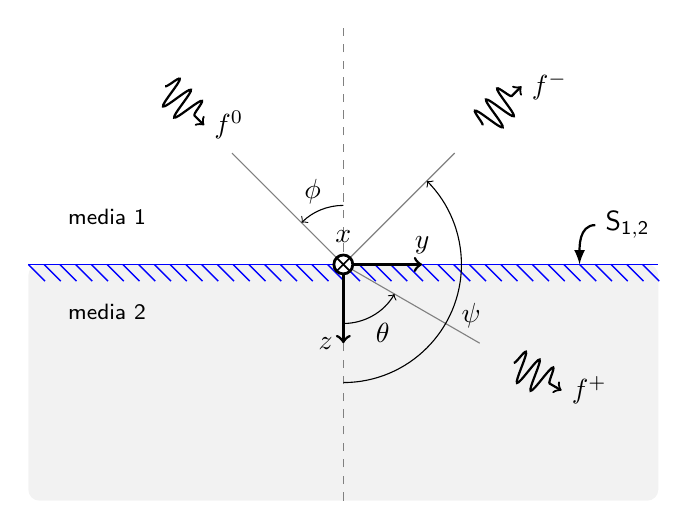
\begin{tikzpicture}[
    media/.style={font={\footnotesize\sffamily}},
    wave/.style={
        decorate,decoration={snake,post length=1.4mm,amplitude=2mm,
        segment length=2mm},thick},
    interface/.style={
        % The border decoration is a path replacing decorator. 
        % For the interface style we want to draw the original path.
        % The postaction option is therefore used to ensure that the
        % border decoration is drawn *after* the original path.
        postaction={draw,decorate,decoration={border,angle=-45,
                    amplitude=0.3cm,segment length=2mm}}},
    ]
    % Round rectangle
    \fill[gray!10,rounded corners] (-4,-3) rectangle (4,0);
    % Interface
    \draw[blue,line width=.5pt,interface](-4,0)--(4,0);
    % Vertical dashed line
    \draw[dashed,gray](0,-3)--(0,3);
    % Coordinates system
    \draw(0,0.15)node[above]{$x$};
    \draw[<->,line width=1pt] (1,0) node[above]{$y$}-|(0,-1) node[left]{$z$};
    % Incidence
    \draw[->,wave]
         (135:3.2cm)--(135:2.5cm)node[right]{$f^0$};
    \draw[gray](0:0cm)--(135:2cm);
    \path (0,0)++(113:1cm)node{$\phi$};
    \draw[->](0,0.75)arc(90:135:.75cm);
    % Transmission
    \draw[->,wave]
         (-30:2.5cm)--(-30:3.2cm)node[right]{$f^+$};
    \draw[gray](0:0cm)--(-30:2cm);
    \path (0,0)++(-60:1cm)node{$\theta$};
    \draw[->] (0,-0.75) arc (-90:-30:.75cm);
    % Reflection
    \draw[->,wave]
         (45:2.5cm)--(45:3.2cm)node[right]{$f^-$};
    \path (0,0)++(-22:1.75cm) node{$\psi$};
    \draw[gray](0:0cm)--(45:2cm);
    \draw[->] (0,-1.5)arc(-90:45:1.5cm);
    % Media names
    \path[media] (-3,.6)  node {media 1}
                 (-3,-.6) node {media 2};

    % $x$ axis
    \filldraw[fill=white,line width=1pt](0,0)circle(.12cm);
    \draw[line width=.6pt] (0,0)
                          +(-135:.12cm) -- +(45:.12cm)
                          +(-45:.12cm) -- +(135:.12cm);
    % Interface pointer
    \draw[-latex,thick](3.2,0.5)node[right]{$\mathsf{S_{1,2}}$}
         to[out=180,in=90] (3,0);
    % To-paths are really useful for drawing curved lines. The above
    % to path is equal to:
    %
    % \draw[-latex,thick](3.2,0.5)node[right]{$\mathsf{S_{1,2}}$}
    %      ..controls +(180:.2cm) and +(up:0.25cm) .. (3,0);
    % Internally the to path is translated to a similar bezier curve,
    % but the to path syntax hides the complexity from the user. 
\end{tikzpicture}%
\end{mdDiv}%%
\end{mdDiv}%
\mdHr[class={figureline,madoko},data-line={1436}]{}\begin{mdDiv}[data-line={1437}]%
% data-line={1437}
{}\mdSpan[class={figure-caption}]{\mdSpan[class={caption-before}]{\mdStrong{Figure{\mdNbsp}\mdSpan[class={figure-label}]{2}.} }\mdA{http://www.texample.net/tikz/examples/oblique-incidence}{}{TikZ example} by Edgar Fuentes of reflection and refraction of electromagnetic waves.}% data-line={1437}
{}%
\end{mdDiv}%%
\end{mdDiv}%
\begin{mdDiv}[class={figure,align-center},id=fig-mergesort,label={[3]\{.figure-label\}},elem={figure},toc={tof},toc-line={[3]\{.figure-label\}. [TikZ example](http://www.texample.net/tikz/examples/merge-sort-recursion-tree) by Manuel Kirsch of a merge sort recursion tree.},caption={[TikZ example](http://www.texample.net/tikz/examples/merge-sort-recursion-tree) by Manuel Kirsch of a merge sort recursion tree.},data-line={1440}]%
\begin{mdDiv}[class={snippet,block,input-math},elem={snippet},snippet-needpdf={true},data-line={1441}]%
\begin{mdDiv}[class={snippet,math-display},snippet-needpdf={true}]%
% data-line={1442}
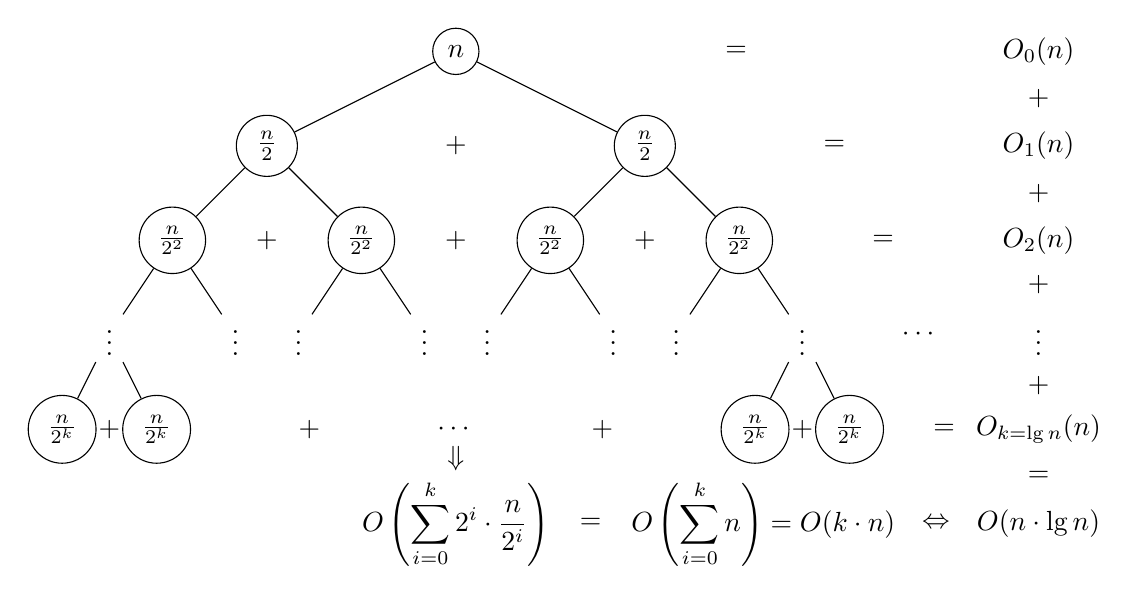
\begin{tikzpicture}[scale=0.8,level/.style={sibling distance=60mm/#1}]
\node [circle,draw] (z){$n$}
  child {node [circle,draw] (a) {$\frac{n}{2}$}
    child {node [circle,draw] (b) {$\frac{n}{2^2}$}
      child {node {$\vdots$}
        child {node [circle,draw] (d) {$\frac{n}{2^k}$}}
        child {node [circle,draw] (e) {$\frac{n}{2^k}$}}
      } 
      child {node {$\vdots$}}
    }
    child {node [circle,draw] (g) {$\frac{n}{2^2}$}
      child {node {$\vdots$}}
      child {node {$\vdots$}}
    }
  }
  child {node [circle,draw] (j) {$\frac{n}{2}$}
    child {node [circle,draw] (k) {$\frac{n}{2^2}$}
      child {node {$\vdots$}}
      child {node {$\vdots$}}
    }
  child {node [circle,draw] (l) {$\frac{n}{2^2}$}
    child {node {$\vdots$}}
    child {node (c){$\vdots$}
      child {node [circle,draw] (o) {$\frac{n}{2^k}$}}
      child {node [circle,draw] (p) {$\frac{n}{2^k}$}
        child [grow=right] {node (q) {$=$} edge from parent[draw=none]
          child [grow=right] {node (q) {$O_{k = \lg n}(n)$} edge from parent[draw=none]
            child [grow=up] {node (r) {$\vdots$} edge from parent[draw=none]
              child [grow=up] {node (s) {$O_2(n)$} edge from parent[draw=none]
                child [grow=up] {node (t) {$O_1(n)$} edge from parent[draw=none]
                  child [grow=up] {node (u) {$O_0(n)$} edge from parent[draw=none]}
                }
              }
            }
            child [grow=down] {node (v) {$O(n \cdot \lg n)$}edge from parent[draw=none]}
          }
        }
      }
    }
  }
};
\path (a) -- (j) node [midway] {+};
\path (b) -- (g) node [midway] {+};
\path (k) -- (l) node [midway] {+};
\path (k) -- (g) node [midway] {+};
\path (d) -- (e) node [midway] {+};
\path (o) -- (p) node [midway] {+};
\path (o) -- (e) node (x) [midway] {$\cdots$}
  child [grow=down] {
    node (y) {$O\left(\displaystyle\sum_{i = 0}^k 2^i \cdot \frac{n}{2^i}\right)$}
    edge from parent[draw=none]
  };
\path (q) -- (r) node [midway] {+};
\path (s) -- (r) node [midway] {+};
\path (s) -- (t) node [midway] {+};
\path (s) -- (l) node [midway] {=};
\path (t) -- (u) node [midway] {+};
\path (z) -- (u) node [midway] {=};
\path (j) -- (t) node [midway] {=};
\path (y) -- (x) node [midway] {$\Downarrow$};
\path (v) -- (y)
  node (w) [midway] {$O\left(\displaystyle\sum_{i = 0}^k n\right) = O(k \cdot n)$};
\path (q) -- (v) node [midway] {=};
\path (e) -- (x) node [midway] {+};
\path (o) -- (x) node [midway] {+};
\path (y) -- (w) node [midway] {$=$};
\path (v) -- (w) node [midway] {$\Leftrightarrow$};
\path (r) -- (c) node [midway] {$\cdots$};
\end{tikzpicture}%
\end{mdDiv}%%
\end{mdDiv}%
\mdHr[class={figureline,madoko},data-line={1512}]{}\begin{mdDiv}[data-line={1513}]%
% data-line={1513}
{}\mdSpan[class={figure-caption}]{\mdSpan[class={caption-before}]{\mdStrong{Figure{\mdNbsp}\mdSpan[class={figure-label}]{3}.} }\mdA{http://www.texample.net/tikz/examples/merge-sort-recursion-tree}{}{TikZ example} by Manuel Kirsch of a merge sort recursion tree.}% data-line={1513}
{}%
\end{mdDiv}%%
\end{mdDiv}%
\begin{mdP}[class={indent},data-line={1516}]%
% data-line={1516}
{}The % data-line={1516}
{}\mdCode[class={code,code1}]{pgfplots}% data-line={1516}
{} library is an extension of TikZ/Pgf to display plots:%
\end{mdP}%
\begin{mdPre}[class={para-block,pre-indented,language-madoko,lang-madoko,madoko,highlighted},language={madoko},data-line={1518}]%
\mdPrecode{\mdToken{Namespace,Metadata,Key,Madoko}{Package:}\mdToken{String,Escape,Madoko}{\prespace{1}pgfplots}}%
\end{mdPre}%
\begin{mdP}[data-line={1520}]%
% data-line={1520}
{}Drawing plots can be done either using math formulas or by giving direct data points:%
\end{mdP}%
\begin{mdDiv}[class={sample},elem={sample},margin-bottom={2ex},data-line={1522}]%
\begin{mdDiv}[class={sampleblock},elem={sampleblock},padding-left={1em},padding-right={1em},padding-top={-1ex},border-style={solid},border-width={1\cssPixel},line-adjust={0},data-line={1523}]%
\begin{mdPre}[class={para-block,samplesource,noescape,pre-fenced},line-adjust={0},data-line={1523},data-line-code={1524}]%
\mdPrecode[data-line={1524}]{Using\prespace{1}the\prespace{1}{`}pgfplots{`}\prespace{1}package\prespace{1}we\prespace{1}can\prespace{1}draw\prespace{1}nice\prespace{1}plots:\prebr{}
{\textasciitilde}\prespace{1}Snippet\prebr{}
{\textbackslash}begin\{tikzpicture\}\prebr{}
{\textbackslash}begin\{axis\}[\prebr{}
\preindent{2}height=8cm,\prebr{}
\preindent{2}width=8cm,\prebr{}
\preindent{2}grid=major,\prebr{}
]\prebr{}
\%\prespace{1}math\prespace{1}plot\prebr{}
{\textbackslash}addplot\prespace{1}\{-x{\textasciicircum}5\prespace{1}-\prespace{1}242\};\prespace{1}\prebr{}
{\textbackslash}addlegendentry\{model\}\prebr{}
\%\prespace{1}data\prespace{1}plot\prebr{}
{\textbackslash}addplot\prespace{1}coordinates\prespace{1}\{\prebr{}
(-4.77778,2027.60977)\prebr{}
(-3.55556,347.84069)\prebr{}
(-2.33333,22.58953)\prebr{}
(-1.11111,-493.50066)\prebr{}
(0.11111,46.66082)\prebr{}
(1.33333,-205.56286)\prebr{}
(2.55556,-341.40638)\prebr{}
(3.77778,-1169.24780)\prebr{}
(5.00000,-3269.56775)\prebr{}
\};\prebr{}
{\textbackslash}addlegendentry\{estimate\}\prebr{}
{\textbackslash}end\{axis\}\prebr{}
{\textbackslash}end\{tikzpicture\}\prebr{}
{\textasciitilde}}%
\end{mdPre}%
\mdHr[class={madoko},width={0.50\linewidth},text-align={left},data-line={1552}]{}\begin{mdP}[data-line={1553}]%
% data-line={1553}
{}Using the % data-line={1553}
{}\mdCode[class={code,code1}]{pgfplots}% data-line={1553}
{} package we can draw nice plots:%
\end{mdP}%
\begin{mdDiv}[class={snippet,block,input-math},elem={snippet},snippet-needpdf={true},data-line={1554}]%
\begin{mdDiv}[class={snippet,math-display},snippet-needpdf={true}]%
% data-line={1555}
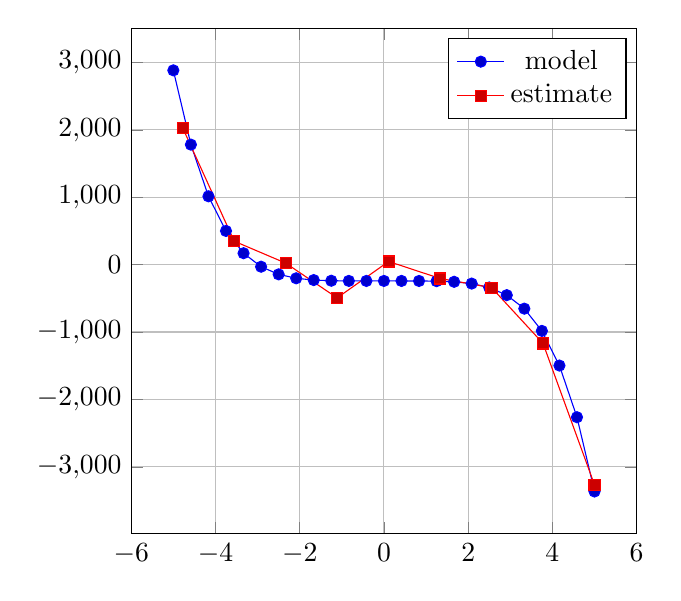
\begin{tikzpicture}
\begin{axis}[
  height=8cm,
  width=8cm,
  grid=major,
]
% math plot
\addplot {-x^5 - 242}; 
\addlegendentry{model}
% data plot
\addplot coordinates {
(-4.77778,2027.60977)
(-3.55556,347.84069)
(-2.33333,22.58953)
(-1.11111,-493.50066)
(0.11111,46.66082)
(1.33333,-205.56286)
(2.55556,-341.40638)
(3.77778,-1169.24780)
(5.00000,-3269.56775)
};
\addlegendentry{estimate}
\end{axis}
\end{tikzpicture}%
\end{mdDiv}%%
\end{mdDiv}%%
\end{mdDiv}%%
\end{mdDiv}%
\begin{mdP}[data-line={1552}]%
% data-line={1552}
{}The final examples in Figure% data-line={1552}
{}{\mdNbsp}\mdA[class={localref},target-element={figure}]{fig-barchart}{}{\mdSpan[class={figure-label}]{4}}% data-line={1552}
{} also use the % data-line={1552}
{}\mdCode[class={code,code1}]{pgfplotstable}% data-line={1552}
{} library:%
\end{mdP}%
\begin{mdPre}[class={para-block,pre-indented,language-madoko,lang-madoko,madoko,highlighted},language={madoko},data-line={1554}]%
\mdPrecode{\mdToken{Namespace,Metadata,Key,Madoko}{Package:}\mdToken{String,Escape,Madoko}{\prespace{1}pgfplotstable}}%
\end{mdPre}%
\begin{mdP}[data-line={1556}]%
% data-line={1556}
{}to display bar charts.%
\end{mdP}%
\begin{mdDiv}[class={figure,align-center},id=fig-barchart,label={[4]\{.figure-label\}},elem={figure},toc={tof},toc-line={[4]\{.figure-label\}. Bar chart examples by [Matt B.][bchart1] and [Jake][bchart2] using `pgfplots`.},caption={Bar chart examples by [Matt B.][bchart1] and [Jake][bchart2] using `pgfplots`.},data-line={1561}]%
\begin{mdTable}[class={columns,block},elem={columns},data-line={1562}]{2}{ll}

\begin{mdColumn}[class={column},elem={column},data-line={1563}]%
\begin{mdDiv}[class={snippet,block,input-math},elem={snippet},snippet-needpdf={true},data-line={1564}]%
\begin{mdDiv}[class={snippet,math-display},snippet-needpdf={true}]%
% data-line={1565}
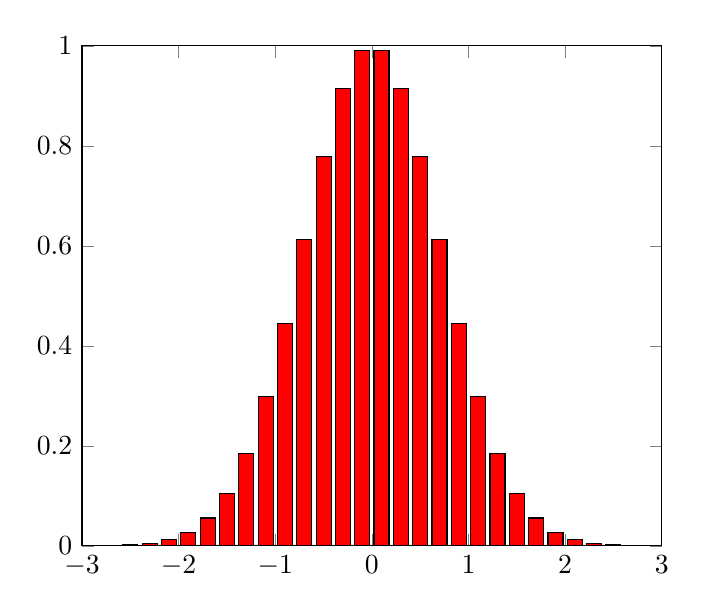
\begin{tikzpicture}
\begin{axis}[%
scale only axis,
height=2.5in,
xmin=-3, xmax=3,
ymin=0, ymax=1,
axis on top]
\addplot[
  ybar,
  bar width=0.075in, 
  bar shift=0in,
  fill=red,
  draw=black] 
  plot coordinates{ 
    (-2.9,0.00022263) (-2.7,0.000682328) (-2.5,0.00193045) (-2.3,0.00504176)
    (-2.1,0.0121552) (-1.9,0.0270518) (-1.7,0.0555762) (-1.5,0.105399)
    (-1.3,0.18452) (-1.1,0.298197) (-0.9,0.444858) (-0.7,0.612626)
    (-0.5,0.778801) (-0.3,0.913931) (-0.1,0.99005) (0.1,0.99005)
    (0.3,0.913931) (0.5,0.778801) (0.7,0.612626) (0.9,0.444858) 
    (1.1,0.298197) (1.3,0.18452) (1.5,0.105399) (1.7,0.0555762)
    (1.9,0.0270518) (2.1,0.0121552) (2.3,0.00504176) (2.5,0.00193045)
    (2.7,0.000682328) (2.9,0.00022263)
  };
\end{axis}
\end{tikzpicture}%
\end{mdDiv}%%
\end{mdDiv}%%
\end{mdColumn}%
&\begin{mdColumn}[class={column},elem={column},vertical-align={bottom},padding-left={2em},data-line={1592}]%
\begin{mdDiv}[class={snippet,block,input-math},elem={snippet},snippet-needpdf={true},data-line={1593}]%
\begin{mdDiv}[class={snippet,math-display},snippet-needpdf={true}]%
% data-line={1594}
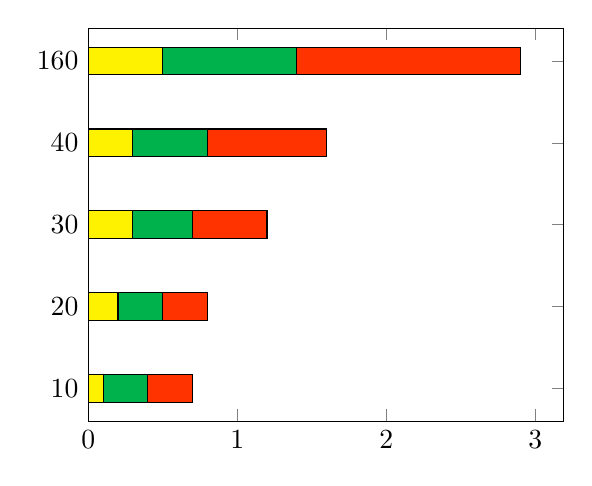
\begin{tikzpicture}
\pgfplotstableread{ % Read the data into a table macro
Label   First   Second  Third
10      0.1     0.3     0.3
20      0.2     0.3     0.3
30      0.3     0.4     0.5
40      0.3     0.5     0.8
160     0.5     0.9     1.5
}\datatable
\begin{axis}[
    width=3in,
    xbar stacked,   % Stacked horizontal bars
    xmin=0,         % Start x axis at 0
    ytick=data,     % Use as many tick labels as y coordinates
    yticklabels from table={\datatable}{Label}  % Get the labels from the Label column of the \datatable
]
\addplot [fill=yellow] table [x=First, y expr=\coordindex] {\datatable};    % Plot the "First" column against the data index
\addplot [fill=green!70!blue]table [x=Second, y expr=\coordindex] {\datatable};
\addplot [fill=red!80!yellow] table [x=Third, y expr=\coordindex] {\datatable};
\end{axis}
\end{tikzpicture}%
\end{mdDiv}%%
\end{mdDiv}%%
\end{mdColumn}%
\\
\end{mdTable}
\mdHr[class={figureline,madoko},data-line={1618}]{}\begin{mdDiv}[data-line={1619}]%
% data-line={1619}
{}\mdSpan[class={figure-caption}]{\mdSpan[class={caption-before}]{\mdStrong{Figure{\mdNbsp}\mdSpan[class={figure-label}]{4}.} }Bar chart examples by{\mdNbsp}\mdA{http://stackoverflow.com/questions/4902147/latex-bar-chart}{}{Matt B.} and{\mdNbsp}\mdA{http://tex.stackexchange.com/questions/99832/how-to-draw-bar-chart-using-tikz}{}{Jake} using \mdCode[class={code,code1}]{pgfplots}.}% data-line={1619}
{}%
\end{mdDiv}%%
\end{mdDiv}%
\mdHxxxx[id=sec-mathefficiency,label={[4.9.5]\{.heading-label\}},toc={},data-line={1620},caption={[[4.9.5]\{.heading-label\}.{\enspace}]\{.heading-before\}Advanced: Efficiency of math rendering},bookmark={4.9.5.{\enspace}Advanced: Efficiency of math rendering}]{% data-line={1620}
{}\mdSpan[class={heading-before}]{\mdSpan[class={heading-label}]{4.9.5}.{\enspace}}% data-line={1620}
{}Advanced: Efficiency of math rendering}\begin{mdP}[data-line={1622}]%
% data-line={1622}
{}Madoko is quite optimized to render mathematics efficiently, especially
for math heavy documents which can easily contain thousands of small 
mathematics fragments. Madoko carefully processes only those fragments
that need recompilation. If needed you can give the % data-line={1625}
{}\mdCode[class={code,code1}]{-r}% data-line={1625}
{} flag to rebuild
everything from scratch.%
\end{mdP}%
\begin{mdP}[class={indent},data-line={1628}]%
% data-line={1628}
{}Usually, Madoko uses plain % data-line={1628}
{}\mdCode[class={code,code1}]{latex}% data-line={1628}
{} to generate a % data-line={1628}
{}\mdCode[class={code,code1}]{.dvi}% data-line={1628}
{} file, and then
uses % data-line={1629}
{}\mdCode[class={code,code1}]{dvipng}% data-line={1629}
{} to extract hi-resolution images, automatically taking care
of proper baseline alignment.%
\end{mdP}%
\begin{mdP}[class={indent},data-line={1632}]%
% data-line={1632}
{}However, certain snippets cannot work with plain % data-line={1632}
{}\mdCode[class={code,code1}]{.dvi}% data-line={1632}
{} and need postscript
or PDF primitives, like the TikZ and PSTricks packages. In such cases,
Madoko will render these snippets using % data-line={1634}
{}\mdCode[class={code,code1}]{xelatex}% data-line={1634}
{} to generate a % data-line={1634}
{}\mdCode[class={code,code1}]{.pdf}% data-line={1634}
{}
file, and% data-line={1635}
{}{\mdNbsp}\mdA{http://www.imagemagick.org/script/binary-releases.php}{}{ImageMagick{'}s Convert}% data-line={1635}
{} program to extract images. However, this
is not done by default since this method is much (much!) slower than extracting
from the % data-line={1637}
{}\mdCode[class={code,code1}]{.dvi}% data-line={1637}
{} file. The % data-line={1637}
{}\mdCode[class={code,code1}]{.pdf}% data-line={1637}
{} method is done automatically for any % data-line={1637}
{}\mdCode[class={code,code1}]{Snippet}% data-line={1637}
{}.
You can force a % data-line={1638}
{}\mdCode[class={code,code1}]{Snippet}% data-line={1638}
{} to use the % data-line={1638}
{}\mdCode[class={code,code1}]{dvi}% data-line={1638}
{} method by setting % data-line={1638}
{}\mdCode[class={code,code1}]{snippet-needspdf=false}% data-line={1638}
{}
in its attributes, and dually, you can force the % data-line={1639}
{}\mdCode[class={code,code1}]{pdf}% data-line={1639}
{} method for any
equation by setting % data-line={1640}
{}\mdCode[class={code,code1}]{math-needspdf=true}% data-line={1640}
{}.%
\end{mdP}%
\mdHxxxx[id=sec-mathpre,label={[4.9.6]\{.heading-label\}},toc={},data-line={1651},caption={[[4.9.6]\{.heading-label\}.{\enspace}]\{.heading-before\}Advanced: Preformatted math},bookmark={4.9.6.{\enspace}Advanced: Preformatted math}]{% data-line={1651}
{}\mdSpan[class={heading-before}]{\mdSpan[class={heading-label}]{4.9.6}.{\enspace}}% data-line={1651}
{}Advanced: Preformatted math}\begin{mdP}[class={para-continue},data-line={1653}]%
% data-line={1653}
{}LaTeX math mode is great for regular mathematics but not so good if one tries
to preserve whitespace or uses longer identifiers. This is actually quite common
for computer science documents where mathematics is mixed with program code.
Madoko supports a % data-line={1656}
{}\mdCode[class={code,code1}]{MathPre}% data-line={1656}
{} custom block that makes % data-line={1656}
{}\mdEm{preformatted}% data-line={1656}
{} math much
easier to typeset. In particular:%
\end{mdP}%
\begin{mdUl}[class={list-star,loose},data-line={1659}]%
\begin{mdLi}[data-line={1659}]%
\begin{mdP}[data-line={1659}]%
% data-line={1659}
{}Whitespace is preserved and spaces are replaced with a medium space (% data-line={1659}
{}\mdCode[class={code,code1}]{{\textbackslash}mathspace}% data-line={1659}
{}) command
  (except when the spaces directly follow a LaTeX command). Indentation is done through
  a % data-line={1661}
{}\mdCode[class={code,code1}]{{\textbackslash}mathindent}% data-line={1661}
{} command, while line breaks are automatic with a % data-line={1661}
{}\mdCode[class={code,code1}]{{\textbackslash}mathbr}% data-line={1661}
{} command.%
\end{mdP}%%
\end{mdLi}%
\begin{mdLi}[data-line={1663}]%
\begin{mdP}[data-line={1663}]%
% data-line={1663}
{}A name (consisting of letters and digits) is typeset in a % data-line={1663}
{}\mdCode[class={code,code1}]{{\textbackslash}mathid}% data-line={1663}
{} command so 
  it will look like % data-line={1664}
{}\mdSpan[class={math-inline},elem={math-inline}]{$\mathit{function}$}% data-line={1664}
{} instead of % data-line={1664}
{}\mdSpan[class={math-inline},elem={math-inline}]{$function$}% data-line={1664}
{} (note the spacing
  between the % data-line={1665}
{}\mdSpan[class={math-inline},elem={math-inline}]{$f$}% data-line={1665}
{} and % data-line={1665}
{}\mdSpan[class={math-inline},elem={math-inline}]{$u$}% data-line={1665}
{} for example).%
\end{mdP}%%
\end{mdLi}%
\begin{mdLi}[data-line={1667}]%
\begin{mdP}[data-line={1667}]%
% data-line={1667}
{}If a name ends with digits, they are typeset as subscripts, where % data-line={1667}
{}\mdCode[class={code,code1}]{x1}% data-line={1667}
{} becomes % data-line={1667}
{}\mdSpan[class={math-inline},elem={math-inline}]{$\mathit{x}_1$}% data-line={1667}
{}.%
\end{mdP}%%
\end{mdLi}%
\begin{mdLi}[data-line={1669}]%
\begin{mdP}[data-line={1669}]%
% data-line={1669}
{}A name starting with an % data-line={1669}
{}\mdCode[class={code,code1}]{@}% data-line={1669}
{} character is typeset using a % data-line={1669}
{}\mdCode[class={code,code1}]{{\textbackslash}mathkw}% data-line={1669}
{} command, where
  % data-line={1670}
{}\mdCode[class={code,code1}]{@return}% data-line={1670}
{} becomes % data-line={1670}
{}\mdSpan[class={math-inline},elem={math-inline}]{$\mathkw{return}$}% data-line={1670}
{}.%
\end{mdP}%%
\end{mdLi}%
\begin{mdLi}[data-line={1672}]%
\begin{mdP}[data-line={1672}]%
% data-line={1672}
{}Any text that is an argument of a % data-line={1672}
{}\mdCode[class={code,code1}]{{\textbackslash}begin}% data-line={1672}
{}, % data-line={1672}
{}\mdCode[class={code,code1}]{{\textbackslash}end}% data-line={1672}
{}, % data-line={1672}
{}\mdCode[class={code,code1}]{{\textbackslash}text}% data-line={1672}
{}\mdEm{xx}% data-line={1672}
{} or
  % data-line={1673}
{}\mdCode[class={code,code1}]{{\textbackslash}math}% data-line={1673}
{}\mdEm{xx}% data-line={1673}
{} command,      where % data-line={1673}
{}\mdEm{xx}% data-line={1673}
{} is one of % data-line={1673}
{}\mdCode[class={code,code1}]{tt}% data-line={1673}
{}, % data-line={1673}
{}\mdCode[class={code,code1}]{sf}% data-line={1673}
{}, % data-line={1673}
{}\mdCode[class={code,code1}]{sl}% data-line={1673}
{}, % data-line={1673}
{}\mdCode[class={code,code1}]{rm}% data-line={1673}
{}, % data-line={1673}
{}\mdCode[class={code,code1}]{it}% data-line={1673}
{},
  % data-line={1674}
{}\mdCode[class={code,code1}]{kw}% data-line={1674}
{}, % data-line={1674}
{}\mdCode[class={code,code1}]{id}% data-line={1674}
{}, % data-line={1674}
{}\mdCode[class={code,code1}]{bb}% data-line={1674}
{}, or % data-line={1674}
{}\mdCode[class={code,code1}]{bf}% data-line={1674}
{}, is kept unchanged. Also any name starting with
  a % data-line={1675}
{}\mdCode[class={code,code1}]{\#}% data-line={1675}
{} character is kept unchanged.%
\end{mdP}%%
\end{mdLi}%
\begin{mdLi}[data-line={1677}]%
\begin{mdP}[data-line={1677}]%
% data-line={1677}
{}Ampersands can be used to align text.%
\end{mdP}%%
\end{mdLi}%%
\end{mdUl}%
\begin{mdP}[data-line={1679}]%
% data-line={1679}
{}Using this convention, we can easily typeset program code using nice symbols.%
\end{mdP}%
\begin{mdDiv}[class={sample},elem={sample},margin-bottom={2ex},data-line={1681}]%
\begin{mdDiv}[class={sampleblock},elem={sampleblock},padding-left={1em},padding-right={1em},padding-top={-1ex},border-style={solid},border-width={1\cssPixel},line-adjust={0},data-line={1682}]%
\begin{mdPre}[class={para-block,samplesource,noescape,pre-fenced},line-adjust={0},data-line={1682},data-line-code={1683}]%
\mdPrecode[data-line={1683}]{{\textasciitilde}\prespace{1}MathPre\prebr{}
@function\prespace{1}sqr\_{\textbackslash}pi(\prespace{1}num\prespace{1}:int\prespace{1})\prespace{1}{\textbackslash}\{\prespace{1}\prebr{}
\preindent{3}@return\prespace{1}(num\prespace{1}\{{\textbackslash}times\}\prespace{1}num\prespace{1}{\textbackslash}times\{\}\prespace{1}{\textbackslash}pi)\prebr{}
{\textbackslash}\}\prespace{2}\prebr{}
{\textasciitilde}}%
\end{mdPre}%
\mdHr[class={madoko},width={0.50\linewidth},text-align={left},data-line={1689}]{}\begin{mdDiv}[class={mathpre,para-block,input-mathpre},elem={mathpre},data-line={1690}]%
\begin{mdDiv}[class={mathpre,math-display}]%
\[% data-line={1691}
\begin{mdMathprearray}%
\mathkw{function}\mathspace{1}\mathid{sqr}_\pi(\mathspace{1}\mathid{num}\mathspace{1}:\mathid{int}\mathspace{1})\mathspace{1}\{\mathspace{1}\mathbr{}
\mathindent{3}\mathkw{return}\mathspace{1}(\mathid{num}\mathspace{1}{\times}\mathspace{1}\mathid{num}\mathspace{1}\times{}\mathspace{1}\pi)\mathbr{}
\}\mathspace{2}
\end{mdMathprearray}\]%
\end{mdDiv}%%
\end{mdDiv}%%
\end{mdDiv}%%
\end{mdDiv}%
\begin{mdP}[data-line={1689}]%
% data-line={1689}
{}Here is an example of aligned text which also demonstrates the use of % data-line={1689}
{}\mdCode[class={code,code1}]{replace}% data-line={1689}
{} (see 
Section% data-line={1690}
{}{\mdNbsp}\mdA[class={localref},target-element={h2}]{sec-replace}{}{\mdSpan[class={heading-label}]{5.6}}% data-line={1690}
{}):%
\end{mdP}%
\begin{mdDiv}[class={sample},elem={sample},margin-bottom={2ex},data-line={1692}]%
\begin{mdDiv}[class={sampleblock},elem={sampleblock},padding-left={1em},padding-right={1em},padding-top={-1ex},border-style={solid},border-width={1\cssPixel},line-adjust={0},data-line={1693}]%
\begin{mdPre}[class={para-block,samplesource,noescape,pre-fenced},line-adjust={0},data-line={1693},data-line-code={1694}]%
\mdPrecode[data-line={1694}]{{\textasciitilde}\prespace{1}MathPre\prespace{3}\{\prespace{1}replace={"}/-{\textgreater}/{\textbackslash}rightarrow/g{"}\prespace{1}\}\prebr{}
random\prespace{1}{\&}:\prespace{1}()\prespace{1}-{\textgreater}\prespace{1}ndet\prespace{1}double;\prespace{1}\prebr{}
print\prespace{2}{\&}:\prespace{1}string\prespace{1}-{\textgreater}\prespace{1}io\prespace{1}();\prebr{}
error\prespace{2}{\&}:\prespace{1}{\textbackslash}forall{\textbackslash}langle{\textbackslash}alpha{\textbackslash}rangle{\textbackslash}\prespace{1}string\prespace{1}-{\textgreater}\prespace{1}exn\prespace{1}{\textbackslash}alpha;\prespace{1}\prebr{}
{\textasciitilde}}%
\end{mdPre}%
\mdHr[class={madoko},width={0.50\linewidth},text-align={left},data-line={1700}]{}\begin{mdDiv}[class={mathpre,para-block,input-mathpre},elem={mathpre},data-line={1701}]%
\begin{mdDiv}[class={mathpre,math-display}]%
\[% data-line={1702}
\begin{mdMathprearray}%
\mathid{random}\mathspace{1}&:\mathspace{1}()\mathspace{1}\rightarrow \mathid{ndet}\mathspace{1}\mathid{double};\mathspace{1}\mathbr{}
\mathid{print}\mathspace{2}&:\mathspace{1}\mathid{string}\mathspace{1}\rightarrow \mathid{io}\mathspace{1}();\mathbr{}
\mathid{error}\mathspace{2}&:\mathspace{1}\forall\langle\alpha\rangle\ \mathid{string}\mathspace{1}\rightarrow \mathid{exn}\mathspace{1}\alpha;\mathspace{1}
\end{mdMathprearray}\]%
\end{mdDiv}%%
\end{mdDiv}%%
\end{mdDiv}%%
\end{mdDiv}%
\begin{mdP}[data-line={1700}]%
% data-line={1700}
{}Of course, you can often achieve a similar effect by using good
replacers with % data-line={1701}
{}\mdCode[class={code,code1}]{.pretty}% data-line={1701}
{} code directly (Section% data-line={1701}
{}{\mdNbsp}\mdA[class={localref},target-element={h3}]{sec-advanced--pretty-code-alignment}{}{\mdSpan[class={heading-label}]{4.7.3}}% data-line={1701}
{}):%
\end{mdP}%
\begin{mdDiv}[class={sample},elem={sample},margin-bottom={2ex},data-line={1703}]%
\begin{mdDiv}[class={sampleblock},elem={sampleblock},padding-left={1em},padding-right={1em},padding-top={-1ex},border-style={solid},border-width={1\cssPixel},line-adjust={0},data-line={1704}]%
\begin{mdPre}[class={para-block,samplesource,noescape,pre-fenced},line-adjust={0},data-line={1704},data-line-code={1705}]%
\mdPrecode[data-line={1705}]{{`}{`}{`}\prespace{1}koka\prespace{3}\{\prespace{1}.pretty\prespace{1}{\textbackslash}\prebr{}
\preindent{13}replace={"}//-{\textgreater}/{\textbackslash}(-{\textgreater}{\textbar}{\&}rarr;{\textbackslash})//{\textless}/{\textbackslash}({\textless}{\textbar}{\&}lang;{\textbackslash})//{\textgreater}/{\textbackslash}({\textgreater}{\textbar}{\&}rang;{\textbackslash})//g{"}\prespace{1}{\textbackslash}\prebr{}
\preindent{13}replace={"}//{\textbackslash}bforall{\textbackslash}b/{\textbackslash}(forall{\textbar}{\&}forall;{\textbackslash})//{\textbackslash}balpha{\textbackslash}b/{\textbackslash}(alpha{\textbar}{\&}alpha;{\textbackslash})//g{"}\prespace{1}\}\prebr{}
random\prespace{2}:\prespace{1}()\prespace{1}-{\textgreater}\prespace{1}ndet\prespace{1}double;\prebr{}
print\prespace{3}:\prespace{1}string\prespace{1}-{\textgreater}\prespace{1}io\prespace{1}();\prebr{}
error\prespace{3}:\prespace{1}forall{\textless}alpha{\textgreater}\prespace{1}string\prespace{1}-{\textgreater}\prespace{1}exn\prespace{1}alpha;\prebr{}
{`}{`}{`}}%
\end{mdPre}%
\mdHr[class={madoko},width={0.50\linewidth},text-align={left},data-line={1713}]{}\begin{mdPre}[class={para-block,pretty,pre-fenced,language-koka,lang-koka,koka,highlighted},data-line={1714},data-line-code={1715},language={koka}]%
\mdPrecode[data-line={1715}]{\begin{mdCodeTable}[data-line={1715}]{2}{ll}
\mdToken{Identifier,Koka}{random}{\prespace{2}}&\mdToken{Type,Operator,Koka}{:}{\prespace{1}}\mdToken{Delimiter,Parenthesis,Koka,Type,BracketOpen}{(}\mdToken{Delimiter,Parenthesis,Koka,Type,BracketClose}{)}{\prespace{1}}\mdToken{Type,Operator,Koka}{\mdSpan[class={code-escaped}]{\ensuremath{\rightarrow}}}{\prespace{1}}\mdToken{Type,Identifier,Koka}{ndet}{\prespace{1}}\mdToken{Type,Identifier,Koka}{double}\mdToken{Delimiter,Koka}{;}\\
\mdToken{Identifier,Koka}{print}{\prespace{3}}&\mdToken{Type,Operator,Koka}{:}{\prespace{1}}\mdToken{Type,Identifier,Koka}{string}{\prespace{1}}\mdToken{Type,Operator,Koka}{\mdSpan[class={code-escaped}]{\ensuremath{\rightarrow}}}{\prespace{1}}\mdToken{Type,Identifier,Koka}{io}{\prespace{1}}\mdToken{Delimiter,Parenthesis,Koka,Type,BracketOpen}{(}\mdToken{Delimiter,Parenthesis,Koka,Type,BracketClose}{)}\mdToken{Delimiter,Koka}{;}\\
\mdToken{Identifier,Predefined,Koka}{error}{\prespace{3}}&\mdToken{Type,Operator,Koka}{:}{\prespace{1}}\mdToken{Type,Keyword,Koka}{\mdSpan[class={code-escaped}]{\ensuremath{\forall}}}\mdToken{Delimiter,Angle,Koka,Type,BracketOpen}{\mdSpan[class={code-escaped}]{\ensuremath{\langle}}}\mdToken{Type,Identifier,Koka}{\mdSpan[class={code-escaped}]{\ensuremath{\alpha}}}\mdToken{Delimiter,Angle,Koka,Type,BracketClose}{\mdSpan[class={code-escaped}]{\ensuremath{\rangle}}}{\prespace{1}}\mdToken{Type,Identifier,Koka}{string}{\prespace{1}}\mdToken{Type,Operator,Koka}{\mdSpan[class={code-escaped}]{\ensuremath{\rightarrow}}}{\prespace{1}}\mdToken{Type,Identifier,Koka}{exn}{\prespace{1}}\mdToken{Type,Identifier,Koka}{\mdSpan[class={code-escaped}]{\ensuremath{\alpha}}}\mdToken{Delimiter,Koka}{;}
\end{mdCodeTable}
}%
\end{mdPre}%%
\end{mdDiv}%%
\end{mdDiv}%
\mdHxxxx[id=sec-setting-all-code-to-preformatted-math,label={[4.9.7]\{.heading-label\}},toc={},data-line={1713},caption={[[4.9.7]\{.heading-label\}.{\enspace}]\{.heading-before\}Setting all code to preformatted math},bookmark={4.9.7.{\enspace}Setting all code to preformatted math}]{% data-line={1713}
{}\mdSpan[class={heading-before}]{\mdSpan[class={heading-label}]{4.9.7}.{\enspace}}% data-line={1713}
{}Setting all code to preformatted math}\begin{mdP}[data-line={1715}]%
% data-line={1715}
{}If you want to typeset all math using preformatted math, you can actually % data-line={1715}
{}{\textquoteleft}take over{\textquoteright}% data-line={1715}
{}
the standard math blocks in Madoko and set the input of those to % data-line={1716}
{}\mdCode[class={code,code1}]{mathpre}% data-line={1716}
{}. 
For example:%
\end{mdP}%
\begin{mdPre}[class={para-block,pre-indented,language-madoko,lang-madoko,madoko,highlighted},language={madoko},data-line={1719}]%
\mdPrecode{\mdToken{Source,Madoko}{.}\mdToken{Source,Madoko}{M}\mdToken{Source,Madoko}{a}\mdToken{Source,Madoko}{t}\mdToken{Source,Madoko}{h}\mdToken{Source,Madoko}{-}\mdToken{Source,Madoko}{I}\mdToken{Source,Madoko}{n}\mdToken{Source,Madoko}{l}\mdToken{Source,Madoko}{i}\mdToken{Source,Madoko}{n}\mdToken{Source,Madoko}{e}\mdToken{Source,Madoko}{,}\mdToken{Source,Madoko}{.}\mdToken{Source,Madoko}{M}\mdToken{Source,Madoko}{a}\mdToken{Source,Madoko}{t}\mdToken{Source,Madoko}{h}\mdToken{Source,Madoko}{-}\mdToken{Source,Madoko}{D}\mdToken{Source,Madoko}{i}\mdToken{Source,Madoko}{s}\mdToken{Source,Madoko}{p}\mdToken{Source,Madoko}{l}\mdToken{Source,Madoko}{a}\mdToken{Source,Madoko}{y}\mdToken{Source,Madoko}{:}{\prespace{1}}\mdToken{Source,Madoko}{i}\mdToken{Source,Madoko}{n}\mdToken{Source,Madoko}{p}\mdToken{Source,Madoko}{u}\mdToken{Source,Madoko}{t}\mdToken{Source,Madoko}{=}\mdToken{Source,Madoko}{m}\mdToken{Source,Madoko}{a}\mdToken{Source,Madoko}{t}\mdToken{Source,Madoko}{h}\mdToken{Source,Madoko}{p}\mdToken{Source,Madoko}{r}\mdToken{Source,Madoko}{e}{\prespace{1}}}%
\end{mdPre}%
\begin{mdP}[data-line={1721}]%
% data-line={1721}
{}These set both display- and inline-math to the % data-line={1721}
{}\mdCode[class={code,code1}]{mathpre}% data-line={1721}
{} input mode.%
\end{mdP}%
\mdHxxx[id=sec-toc,label={[4.10]\{.heading-label\}},toc={},data-line={1724},caption={[[4.10]\{.heading-label\}.{\enspace}]\{.heading-before\}Table of contents},bookmark={4.10.{\enspace}Table of contents}]{% data-line={1724}
{}\mdSpan[class={heading-before}]{\mdSpan[class={heading-label}]{4.10}.{\enspace}}% data-line={1724}
{}Table of contents}\begin{mdP}[data-line={1726}]%
% data-line={1726}
{}Generating a table of contents is easy, just include the special element
% data-line={1727}
{}\mdCode[class={code,code1}]{[TOC]}% data-line={1727}
{} anywhere in your document and it will expand to a table of contents.
You an use the metadata value % data-line={1728}
{}\mdCode[class={code,code1}]{Toc\prespace{1}Depth}% data-line={1728}
{} to set how many levels deep the
table of contents goes (by default 3).%
\end{mdP}%
\begin{mdP}[class={indent},data-line={1731}]%
% data-line={1731}
{}You can also a create a list of figures, by using % data-line={1731}
{}\mdCode[class={code,code1}]{[TOC=tof]}% data-line={1731}
{}. This will list
all the % data-line={1732}
{}\mdCode[class={code,code1}]{{\textasciitilde}Figure}% data-line={1732}
{} block elements.%
\end{mdP}%
\mdHxxxx[id=sec-advanced--custom-tables-of-contents,label={[4.10.1]\{.heading-label\}},toc={},data-line={1734},caption={[[4.10.1]\{.heading-label\}.{\enspace}]\{.heading-before\}Advanced: Custom tables of contents},bookmark={4.10.1.{\enspace}Advanced: Custom tables of contents}]{% data-line={1734}
{}\mdSpan[class={heading-before}]{\mdSpan[class={heading-label}]{4.10.1}.{\enspace}}% data-line={1734}
{}Advanced: Custom tables of contents}\begin{mdP}[data-line={1736}]%
% data-line={1736}
{}Custom tables of contents can be generated using the % data-line={1736}
{}\mdCode[class={code,code1}]{toc}% data-line={1736}
{} attribute.  The
% data-line={1737}
{}\mdCode[class={code,code1}]{toc-depth}% data-line={1737}
{} attribute specifies the depth of the element (by default 1), while
the % data-line={1738}
{}\mdCode[class={code,code1}]{toc-line}% data-line={1738}
{} specifies the contents of the line displayed in the table of
contents. For example, using% data-line={1739}
{}{\mdNbsp}\mdA[class={localref},target-element={h2}]{sec-rules}{}{metadata rules}% data-line={1739}
{} we can generate a
table of contents for equations:%
\end{mdP}%
\begin{mdPre}[class={para-block,pre-indented,language-madoko,lang-madoko,madoko,highlighted},language={madoko},data-line={1742}]%
\mdPrecode{\mdToken{Namespace,Metadata,Key,Madoko}{{\textasciitilde}Equation:}\mdToken{String,Escape,Madoko}{\prespace{1}toc=equations\prespace{1}toc-line={"}{\&}caption;{"}}}%
\end{mdPre}%
\begin{mdP}[data-line={1744}]%
% data-line={1744}
{}Here we assume that the user adds a % data-line={1744}
{}\mdCode[class={code,code1}]{caption}% data-line={1744}
{} attribute when denoting
equations (which will get expanded inside the % data-line={1745}
{}\mdCode[class={code,code1}]{toc-line}% data-line={1745}
{}). We can then render
the table of equations anywhere in the document as:%
\end{mdP}%
\begin{mdPre}[class={para-block,pre-indented,language-madoko,lang-madoko,madoko,highlighted},language={madoko},data-line={1748}]%
\mdPrecode{\mdToken{String,Link,Madoko}{[TOC=equations]}}%
\end{mdPre}%
\mdHxxx[id=sec-bib,label={[4.11]\{.heading-label\}},toc={},data-line={1750},caption={[[4.11]\{.heading-label\}.{\enspace}]\{.heading-before\}Bibliography and Citations},bookmark={4.11.{\enspace}Bibliography and Citations}]{% data-line={1750}
{}\mdSpan[class={heading-before}]{\mdSpan[class={heading-label}]{4.11}.{\enspace}}% data-line={1750}
{}Bibliography and Citations}\begin{mdP}[data-line={1752}]%
% data-line={1752}
{}One of Madoko% data-line={1752}
{}{'}% data-line={1752}
{}s main design goals is to enable the creation of high-quality
scholarly articles. As such, Madoko integrates closely with the standard 
% data-line={1754}
{}\mdA{http://en.wikipedia.org/wiki/BibTeX}{}{BibTeX}% data-line={1754}
{} tool to generate bibliographies and references inside a document.
Usually, BibTeX comes standard with any LaTeX installation.%
\end{mdP}%
\begin{mdP}[class={indent},data-line={1757}]%
% data-line={1757}
{}You can simply use any existing BibTeX bibliography file (% data-line={1757}
{}\mdCode[class={code,code1}]{.bib}% data-line={1757}
{}). You can
specify which bibliography files are to be used using  % data-line={1758}
{}\mdCode[class={code,code1}]{Bib}% data-line={1758}
{} 
% data-line={1759}
{}\mdA[class={localref}]{sec-metadata}{}{metadata}% data-line={1759}
{} entries:%
\end{mdP}%
\begin{mdPre}[class={para-block,pre-indented,language-madoko,lang-madoko,madoko,highlighted},language={madoko},data-line={1761}]%
\mdPrecode{\mdToken{Namespace,Metadata,Key,Madoko}{Bib:}\mdToken{String,Escape,Madoko}{\prespace{2}../mybib1}\prebr{}
\mdToken{Namespace,Metadata,Key,Madoko}{Bib:}\mdToken{String,Escape,Madoko}{\prespace{2}mybib2}}%
\end{mdPre}%
\begin{mdP}[data-line={1764}]%
% data-line={1764}
{} 
As an example, you can view the bibliography for this document% data-line={1765}
{}{\mdNbsp}\mdA{reference.bib}{}{here}% data-line={1765}
{}.
Entries in the bibliography files can now be referenced using semi-colon separated 
references (as in% data-line={1767}
{}{\mdNbsp}\mdA{http://johnmacfarlane.net/pandoc}{}{Pandoc}% data-line={1767}
{}), for example%
\end{mdP}%
\begin{mdDiv}[class={sample},elem={sample},margin-bottom={2ex},data-line={1768}]%
\begin{mdDiv}[class={sampleblock},elem={sampleblock},padding-left={1em},padding-right={1em},padding-top={-1ex},border-style={solid},border-width={1\cssPixel},line-adjust={0},data-line={1769}]%
\begin{mdPre}[class={para-block,samplesource,noescape,pre-fenced},line-adjust={0},data-line={1769},data-line-code={1770}]%
\mdPrecode[data-line={1770}]{Read\prespace{1}about\prespace{1}LaTeX\prespace{1}and\prespace{1}TeX\prespace{1}[@Knuth:Tex;\prespace{1}@Lamport:Latex].}%
\end{mdPre}%
\mdHr[class={madoko},width={0.50\linewidth},text-align={left},data-line={1772}]{}\begin{mdP}[data-line={1773}]%
% data-line={1773}
{}Read about LaTeX and TeX% data-line={1773}
{}{\mdNbsp}\mdSpan[class={citations},target-element={bibitem}]{[\mdA[class={bibref,localref},target-element={bibitem}]{knuth:tex}{}{\mdSpan[class={bibitem-label}]{4}}, \mdA[class={bibref,localref},target-element={bibitem}]{lamport:latex}{}{\mdSpan[class={bibitem-label}]{5}}]}% data-line={1773}
{}.%
\end{mdP}%%
\end{mdDiv}%%
\end{mdDiv}%
\begin{mdP}[data-line={1772}]%
% data-line={1772}
{}Note that unlike LaTeX there is no need to explicitly insert an unbreakable
space between the text and the citation, Madoko automatically takes care of this
(as described in Section% data-line={1774}
{}{\mdNbsp}\mdA[class={localref},target-element={h2}]{sec-ids-labels}{}{\mdSpan[class={heading-label}]{4.2}}% data-line={1774}
{}).
If necessary, you can also include extra text for each entry:%
\end{mdP}%
\begin{mdDiv}[class={sample},elem={sample},margin-bottom={2ex},data-line={1777}]%
\begin{mdDiv}[class={sampleblock},elem={sampleblock},padding-left={1em},padding-right={1em},padding-top={-1ex},border-style={solid},border-width={1\cssPixel},line-adjust={0},data-line={1778}]%
\begin{mdPre}[class={para-block,samplesource,noescape,pre-fenced},line-adjust={0},data-line={1778},data-line-code={1779}]%
\mdPrecode[data-line={1779}]{Read\prespace{1}more\prespace{1}[The\prespace{1}book\prespace{1}@Knuth:Tex;{\textbackslash}\prespace{1}@Lamport:Latex\prespace{1}(chapter\prespace{1}4)].\prespace{1}}%
\end{mdPre}%
\mdHr[class={madoko},width={0.50\linewidth},text-align={left},data-line={1781}]{}\begin{mdP}[data-line={1782}]%
% data-line={1782}
{}Read more% data-line={1782}
{}{\mdNbsp}\mdSpan[class={citations},target-element={bibitem}]{[The book{\mdNbsp}\mdA[class={bibref,localref},target-element={bibitem}]{knuth:tex}{}{\mdSpan[class={bibitem-label}]{4}}, {\mdNbsp}\mdA[class={bibref,localref},target-element={bibitem}]{lamport:latex}{}{\mdSpan[class={bibitem-label}]{5}} (chapter 4)]}% data-line={1782}
{}.%
\end{mdP}%%
\end{mdDiv}%%
\end{mdDiv}%
\begin{mdP}[data-line={1781}]%
% data-line={1781}
{}When Madoko finds such references, it writes them to a % data-line={1781}
{}\mdCode[class={code,code1}]{.bib.aux}% data-line={1781}
{} file
(together with the needed bibliography files) that are read by BibTeX to
generate the bibliography entries. BibTeX is called automatically by Madoko
whenever the citations change. The generated bibliography entries are included
in your document using the special % data-line={1785}
{}\mdCode[class={code,code1}]{[BIB]}% data-line={1785}
{} element, for example:%
\end{mdP}%
\begin{mdPre}[class={para-block,pre-indented,language-madoko,lang-madoko,madoko,highlighted},language={madoko},data-line={1787}]%
\mdPrecode{\mdToken{Keyword,Madoko}{\#\#}\mdToken{Keyword,Madoko}{\prespace{1}References\prespace{3}}\mdToken{String,Escape,Madoko}{\{-\}}\prebr{}
\mdToken{String,Link,Madoko}{[BIB]}}%
\end{mdPre}%
\begin{mdP}[data-line={1790}]%
% data-line={1790}
{}which you can see at the% data-line={1790}
{}{\mdNbsp}\mdA[class={localref},target-element={h1}]{sec-references}{}{end of this document}% data-line={1790}
{}.%
\end{mdP}%
\mdHxxxx[id=sec-bibstyle,label={[4.11.1]\{.heading-label\}},toc={},data-line={1792},caption={[[4.11.1]\{.heading-label\}.{\enspace}]\{.heading-before\}Bibliography styles},bookmark={4.11.1.{\enspace}Bibliography styles}]{% data-line={1792}
{}\mdSpan[class={heading-before}]{\mdSpan[class={heading-label}]{4.11.1}.{\enspace}}% data-line={1792}
{}Bibliography styles}\begin{mdP}[data-line={1794}]%
% data-line={1794}
{}The style of the bibliography entries is determined using the % data-line={1794}
{}\mdCode[class={code,code1}]{Bib\prespace{1}Style}% data-line={1794}
{} key
and can be any% data-line={1795}
{}{\mdNbsp}\mdA{http://web.reed.edu/cis/help/latex/bibtexstyles.html}{}{BibTeX style}% data-line={1795}
{}
(by default % data-line={1796}
{}\mdCode[class={code,code1}]{plainnat}% data-line={1796}
{}):%
\end{mdP}%
\begin{mdPre}[class={para-block,pre-indented,language-madoko,lang-madoko,madoko,highlighted},language={madoko},data-line={1798}]%
\mdPrecode{\mdToken{Namespace,Metadata,Key,Madoko}{Bib\prespace{1}Style:}\mdToken{String,Escape,Madoko}{\prespace{1}abbrvnat}}%
\end{mdPre}%
\begin{mdP}[data-line={1800}]%
% data-line={1800}
{}Madoko uses a very simple LaTeX parser to format the bibliography entries in
Markdown. It can handle things like special characters and accents quite well
and recognizes many formatting commands. Even though it is sufficient for
bibliography entries in general, the Madoko LaTeX parser may not work for more
fancy LaTeX commands in bibliography entries. However, we strive to make it
work for any bibliograpy style and entries, so please% data-line={1805}
{}{\mdNbsp}\mdA{http://madoko.codeplex.com/workitem/list/basic}{}{file a bug report}% data-line={1805}
{} 
if you encounter situations where it does not work correctly.%
\end{mdP}%
\begin{mdP}[class={indent},data-line={1808}]%
% data-line={1808}
{}Bibliography styles tested with Madoko include the following author-year
styles: % data-line={1809}
{}\mdCode[class={code,code1}]{apa}% data-line={1809}
{}, % data-line={1809}
{}\mdCode[class={code,code1}]{apalike}% data-line={1809}
{}, % data-line={1809}
{}\mdCode[class={code,code1}]{plainnat}% data-line={1809}
{}, % data-line={1809}
{}\mdCode[class={code,code1}]{abbrvnat}% data-line={1809}
{}, % data-line={1809}
{}\mdCode[class={code,code1}]{unsrtnat}% data-line={1809}
{}, % data-line={1809}
{}\mdCode[class={code,code1}]{newapa}% data-line={1809}
{},
% data-line={1810}
{}\mdCode[class={code,code1}]{chicago}% data-line={1810}
{}, % data-line={1810}
{}\mdCode[class={code,code1}]{named}% data-line={1810}
{},  % data-line={1810}
{}\mdCode[class={code,code1}]{agsm}% data-line={1810}
{}, % data-line={1810}
{}\mdCode[class={code,code1}]{dcu}% data-line={1810}
{}, % data-line={1810}
{}\mdCode[class={code,code1}]{kluwer}% data-line={1810}
{}, % data-line={1810}
{}\mdCode[class={code,code1}]{astron}% data-line={1810}
{}, % data-line={1810}
{}\mdCode[class={code,code1}]{bbs}% data-line={1810}
{}, % data-line={1810}
{}\mdCode[class={code,code1}]{cbe}% data-line={1810}
{},
% data-line={1811}
{}\mdCode[class={code,code1}]{humannat}% data-line={1811}
{}, % data-line={1811}
{}\mdCode[class={code,code1}]{humanbio}% data-line={1811}
{}, % data-line={1811}
{}\mdCode[class={code,code1}]{jtb}% data-line={1811}
{}, % data-line={1811}
{}\mdCode[class={code,code1}]{apsrev4-1}% data-line={1811}
{}, % data-line={1811}
{}\mdCode[class={code,code1}]{aipauth4-1}% data-line={1811}
{} and others. 
Also, the following numeric styles
have been tested: % data-line={1813}
{}\mdCode[class={code,code1}]{eptcs}% data-line={1813}
{},  % data-line={1813}
{}\mdCode[class={code,code1}]{abbrv}% data-line={1813}
{}, % data-line={1813}
{}\mdCode[class={code,code1}]{plain}% data-line={1813}
{}, % data-line={1813}
{}\mdCode[class={code,code1}]{ieeetr}% data-line={1813}
{}, % data-line={1813}
{}\mdCode[class={code,code1}]{acm}% data-line={1813}
{}, % data-line={1813}
{}\mdCode[class={code,code1}]{unsrt}% data-line={1813}
{},
% data-line={1814}
{}\mdCode[class={code,code1}]{alpha}% data-line={1814}
{}, % data-line={1814}
{}\mdCode[class={code,code1}]{siam}% data-line={1814}
{}, % data-line={1814}
{}\mdCode[class={code,code1}]{apsrmp4-1}% data-line={1814}
{}, % data-line={1814}
{}\mdCode[class={code,code1}]{aipnum4-1}% data-line={1814}
{} and others.
Since tools like BibTeX and Madoko make numbering and linking automatic,  it
is generally preferred for modern documents to use a numeric citations style.%
\end{mdP}%
\mdHxxxx[id=sec-cite,label={[4.11.2]\{.heading-label\}},toc={},data-line={1822},caption={[[4.11.2]\{.heading-label\}.{\enspace}]\{.heading-before\}Citation styles},bookmark={4.11.2.{\enspace}Citation styles}]{% data-line={1822}
{}\mdSpan[class={heading-before}]{\mdSpan[class={heading-label}]{4.11.2}.{\enspace}}% data-line={1822}
{}Citation styles}\begin{mdP}[data-line={1824}]%
% data-line={1824}
{}The citation style defaults to a % data-line={1824}
{}\mdEm{numeric}% data-line={1824}
{} style. However, it can be set
explicitly using the % data-line={1825}
{}\mdCode[class={code,code1}]{Cite\prespace{1}Style}% data-line={1825}
{} metadata key:%
\end{mdP}%
\begin{mdPre}[class={para-block,pre-indented,language-madoko,lang-madoko,madoko,highlighted},language={madoko},data-line={1827}]%
\mdPrecode{\mdToken{Namespace,Metadata,Key,Madoko}{Cite\prespace{1}Style:}\mdToken{String,Escape,Madoko}{\prespace{1}natural}}%
\end{mdPre}%
\begin{mdP}[data-line={1829}]%
% data-line={1829}
{}Valid citation styles are % data-line={1829}
{}\mdEm{natural}% data-line={1829}
{}, % data-line={1829}
{}\mdEm{textual}% data-line={1829}
{}, % data-line={1829}
{}\mdEm{super}% data-line={1829}
{},
and % data-line={1830}
{}\mdEm{numeric}% data-line={1830}
{} (default). The natural and textual style use author-year style
citations, while the super and numeric styles use numbers.%
\end{mdP}%
\begin{mdTable}[class={madoko,block},data-line={1833}]{3}{lll}

\mdTd[data-line={1834},display={table-cell}]{% data-line={1834}
{} % data-line={1834}
{}\mdEm{natural}% data-line={1834}
{}}&\mdTd[data-line={1834},display={table-cell}]{% data-line={1834}
{}{\mdNbsp}\mdSpan[class={citations},cite-style={natural},target-element={bibitem}]{(Lamport,{\mdNbsp}\mdA[class={bibref,localref},target-element={bibitem}]{lamport:latex}{}{1994}; Knuth,{\mdNbsp}\mdA[class={bibref,localref},target-element={bibitem}]{knuth:tex}{}{1984})}% data-line={1834}
{}}&\mdTd[data-line={1834},display={table-cell}]{% data-line={1834}
{} (default for author-year citations)}\\
\mdTd[data-line={1835},display={table-cell}]{% data-line={1835}
{} % data-line={1835}
{}\mdEm{textual}% data-line={1835}
{}}&\mdTd[data-line={1835},display={table-cell}]{% data-line={1835}
{}{\mdNbsp}\mdSpan[class={citations},cite-style={textual},target-element={bibitem}]{Lamport{\mdNbsp}(\mdA[class={bibref,localref},target-element={bibitem}]{lamport:latex}{}{1994}); Knuth{\mdNbsp}(\mdA[class={bibref,localref},target-element={bibitem}]{knuth:tex}{}{1984})}% data-line={1835}
{}}&\mdTd[data-line={1835},display={table-cell}]{% data-line={1835}
{}}\\
\mdTd[data-line={1836},display={table-cell}]{% data-line={1836}
{} % data-line={1836}
{}\mdEm{numeric}% data-line={1836}
{}}&\mdTd[data-line={1836},display={table-cell}]{% data-line={1836}
{}{\mdNbsp}\mdSpan[class={citations},cite-style={numeric},target-element={bibitem}]{[\mdA[class={bibref,localref},target-element={bibitem}]{knuth:tex}{}{\mdSpan[class={bibitem-label}]{4}}, \mdA[class={bibref,localref},target-element={bibitem}]{lamport:latex}{}{\mdSpan[class={bibitem-label}]{5}}]}% data-line={1836}
{}}&\mdTd[data-line={1836},display={table-cell}]{% data-line={1836}
{} (default for numeric citations)}\\
\mdTd[data-line={1837},display={table-cell}]{% data-line={1837}
{} % data-line={1837}
{}\mdEm{super}% data-line={1837}
{}}&\mdTd[data-line={1837},display={table-cell}]{% data-line={1837}
{}{\mdNbsp}\mdSpan[class={citations},cite-style={super},target-element={bibitem}]{\mdSup{\mdA[class={bibref,localref},target-element={bibitem}]{knuth:tex}{}{\mdSpan[class={bibitem-label}]{4}},\mdA[class={bibref,localref},target-element={bibitem}]{lamport:latex}{}{\mdSpan[class={bibitem-label}]{5}}}}% data-line={1837}
{}}&\mdTd[data-line={1837},display={table-cell}]{% data-line={1837}
{}}\\
\end{mdTable}
\begin{mdP}[data-line={1839}]%
% data-line={1839}
{}Note that numeric citations are sorted (and compressed) by default.
Also full author-year style citations only work with BibTeX styles that
support this, i.e. generally any style that works with the % data-line={1841}
{}\mdCode[class={code,code1}]{natbib}% data-line={1841}
{} package
like % data-line={1842}
{}\mdCode[class={code,code1}]{plainnat}% data-line={1842}
{}. With author-year citations we can use modifiers to change how 
the citation is shown. For example, assuming a % data-line={1843}
{}\mdEm{natural}% data-line={1843}
{} style:%
\end{mdP}%
\begin{mdTable}[class={madoko,block},data-line={1845}]{3}{lll}

\mdTd[data-line={1846},display={table-cell}]{% data-line={1846}
{} % data-line={1846}
{}\mdCode[class={code,code1}]{[@Goo93]}% data-line={1846}
{}}&\mdTd[data-line={1846},display={table-cell}]{% data-line={1846}
{}{\mdNbsp}\mdSpan[class={citations},cite-style={natural},target-element={bibitem}]{(Goossens et{\mdNbsp}al.,{\mdNbsp}\mdA[class={bibref,localref},target-element={bibitem}]{goo93}{}{1993})}% data-line={1846}
{}}&\mdTd[data-line={1846},display={table-cell}]{% data-line={1846}
{} Natural}\\
\mdTd[data-line={1847},display={table-cell}]{% data-line={1847}
{} % data-line={1847}
{}\mdCode[class={code,code1}]{[+@Goo93]}% data-line={1847}
{}}&\mdTd[data-line={1847},display={table-cell}]{% data-line={1847}
{}{\mdNbsp}\mdSpan[class={citations},cite-style={natural},target-element={bibitem}]{(Goossens, Mittelbach, and Samarin,{\mdNbsp}\mdA[class={bibref,localref},target-element={bibitem}]{goo93}{}{1993})}% data-line={1847}
{}}&\mdTd[data-line={1847},display={table-cell}]{% data-line={1847}
{} Long% data-line={1847}
{} % data-line={1847}
{}{\textendash}% data-line={1847}
{} all authors}\\
\mdTd[data-line={1848},display={table-cell}]{% data-line={1848}
{} % data-line={1848}
{}\mdCode[class={code,code1}]{[-@Goo93]}% data-line={1848}
{}}&\mdTd[data-line={1848},display={table-cell}]{% data-line={1848}
{}{\mdNbsp}\mdSpan[class={citations},cite-style={natural},target-element={bibitem}]{(\mdA[class={bibref,localref},target-element={bibitem}]{goo93}{}{1993})}% data-line={1848}
{}}&\mdTd[data-line={1848},display={table-cell}]{% data-line={1848}
{} Short% data-line={1848}
{} % data-line={1848}
{}{\textendash}% data-line={1848}
{} just year}\\
\end{mdTable}
\begin{mdP}[data-line={1850}]%
% data-line={1850}
{}Moreover, if you leave out the brackets, you force a % data-line={1850}
{}\mdEm{textual}% data-line={1850}
{} style:%
\end{mdP}%
\begin{mdTable}[class={madoko,block},data-line={1852}]{3}{lll}

\mdTd[data-line={1853},display={table-cell}]{% data-line={1853}
{} % data-line={1853}
{}\mdCode[class={code,code1}]{@Goo93}% data-line={1853}
{}}&\mdTd[data-line={1853},display={table-cell}]{% data-line={1853}
{}{\mdNbsp}\mdSpan[class={textual,citations},cite-style={natural},target-element={bibitem}]{Goossens et{\mdNbsp}al.{\mdNbsp}(\mdA[class={bibref,localref},target-element={bibitem}]{goo93}{}{1993})}% data-line={1853}
{}}&\mdTd[data-line={1853},display={table-cell}]{% data-line={1853}
{} Textual style}\\
\mdTd[data-line={1854},display={table-cell}]{% data-line={1854}
{} % data-line={1854}
{}\mdCode[class={code,code1}]{+@Goo93}% data-line={1854}
{}}&\mdTd[data-line={1854},display={table-cell}]{% data-line={1854}
{}{\mdNbsp}\mdSpan[class={textual,citations},cite-style={natural},target-element={bibitem}]{Goossens, Mittelbach, and Samarin{\mdNbsp}(\mdA[class={bibref,localref},target-element={bibitem}]{goo93}{}{1993})}% data-line={1854}
{}}&\mdTd[data-line={1854},display={table-cell}]{% data-line={1854}
{} Long% data-line={1854}
{} % data-line={1854}
{}{\textendash}% data-line={1854}
{} all authors}\\
\mdTd[data-line={1855},display={table-cell}]{% data-line={1855}
{} % data-line={1855}
{}\mdCode[class={code,code1}]{-@Goo93}% data-line={1855}
{}}&\mdTd[data-line={1855},display={table-cell}]{% data-line={1855}
{}{\mdNbsp}\mdSpan[class={textual,citations},cite-style={natural},target-element={bibitem}]{\mdA[class={bibref,localref},target-element={bibitem}]{goo93}{}{1993}}% data-line={1855}
{}}&\mdTd[data-line={1855},display={table-cell}]{% data-line={1855}
{} Short% data-line={1855}
{} % data-line={1855}
{}{\textendash}% data-line={1855}
{} just year}\\
\mdTd[data-line={1856},display={table-cell}]{% data-line={1856}
{} % data-line={1856}
{}\mdCode[class={code,code1}]{!@Goo93}% data-line={1856}
{}}&\mdTd[data-line={1856},display={table-cell}]{% data-line={1856}
{}{\mdNbsp}\mdSpan[class={textual,citations},cite-style={natural},target-element={bibitem}]{Goossens et{\mdNbsp}al.}% data-line={1856}
{}}&\mdTd[data-line={1856},display={table-cell}]{% data-line={1856}
{} Just authors}\\
\end{mdTable}
\begin{mdP}[data-line={1858}]%
% data-line={1858}
{}In a numeric style, most of these attibutes have no effect and all the 
bracketed cases are displayed as % data-line={1859}
{}{\textquotedblleft}\mdSpan[class={citations},target-element={bibitem}]{[\mdA[class={bibref,localref},target-element={bibitem}]{goo93}{}{\mdSpan[class={bibitem-label}]{2}}]}{\textquotedblright}% data-line={1859}
{}. 
For the four cases in textual style, we get  % data-line={1860}
{}{\textquotedblleft}\mdSpan[class={textual,citations},target-element={bibitem}]{Goossens et{\mdNbsp}al.{\mdNbsp}[\mdA[class={bibref,localref},target-element={bibitem}]{goo93}{}{\mdSpan[class={bibitem-label}]{2}}]}{\textquotedblright}% data-line={1860}
{}, % data-line={1860}
{}{\textquotedblleft}\mdSpan[class={textual,citations},target-element={bibitem}]{Goossens, Mittelbach, and Samarin{\mdNbsp}[\mdA[class={bibref,localref},target-element={bibitem}]{goo93}{}{\mdSpan[class={bibitem-label}]{2}}]}{\textquotedblright}% data-line={1860}
{}, % data-line={1860}
{}{\textquotedblleft}\mdSpan[class={textual,free,citations},target-element={bibitem}]{\mdA[class={bibref,localref},target-element={bibitem}]{goo93}{}{\mdSpan[class={bibitem-label}]{2}}}{\textquotedblright}% data-line={1860}
{}, and % data-line={1860}
{}{\textquotedblleft}\mdSpan[class={textual,citations},target-element={bibitem}]{Goossens et{\mdNbsp}al.}{\textquotedblright}% data-line={1860}
{}.%
\end{mdP}%
\begin{mdP}[class={indent},data-line={1862}]%
% data-line={1862}
{}See Appendix% data-line={1862}
{}{\mdNbsp}\mdA[class={localref},target-element={h2}]{sec-custom-cite}{}{\mdSpan[class={heading-label}]{A.3}}% data-line={1862}
{} on how to customize citations styles further,
and Appendix% data-line={1863}
{}{\mdNbsp}\mdA[class={localref},target-element={h2}]{sec-custom-bib}{}{\mdSpan[class={heading-label}]{A.4}}% data-line={1863}
{} on how to write your bibliography entries
by hand without using BibTeX.%
\end{mdP}%
\mdHxxxx[id=sec-bibliography-tooltips-and-searches,label={[4.11.3]\{.heading-label\}},toc={},data-line={1866},caption={[[4.11.3]\{.heading-label\}.{\enspace}]\{.heading-before\}Bibliography tooltips and searches},bookmark={4.11.3.{\enspace}Bibliography tooltips and searches}]{% data-line={1866}
{}\mdSpan[class={heading-before}]{\mdSpan[class={heading-label}]{4.11.3}.{\enspace}}% data-line={1866}
{}Bibliography tooltips and searches}\begin{mdP}[data-line={1868}]%
% data-line={1868}
{}By default, the HTML backend shows a tooltip when hovering over  a citation
(try it% data-line={1869}
{}{\mdNbsp}\mdSpan[class={citations},target-element={bibitem}]{[\mdA[class={bibref,localref},target-element={bibitem}]{goo93}{}{\mdSpan[class={bibitem-label}]{2}}]}% data-line={1869}
{}). This functionality is by default disabled in the LaTeX
backend. However, you can enable tooltips in PDF too by setting the
% data-line={1871}
{}\mdCode[class={code,code1}]{.tex-tooltip}% data-line={1871}
{} class through a metadata rule:%
\end{mdP}%
\begin{mdPre}[class={para-block,pre-indented,language-madoko,lang-madoko,madoko,highlighted},language={madoko},data-line={1873}]%
\mdPrecode{\mdToken{Namespace,Metadata,Key,Madoko}{{\textasciitilde}a:}\mdToken{String,Escape,Madoko}{\prespace{1}.tex-tooltip}}%
\end{mdPre}%
\begin{mdP}[data-line={1875}]%
% data-line={1875}
{}This will display a small yellow text baloon in the PDF file that shows a
tooltip when hovering above it:%
\end{mdP}%
\begin{mdDiv}[class={center,align-center},elem={center},data-line={1878}]%
\begin{mdP}[data-line={1879}]%
% data-line={1879}
{}\mdImg[width={300\cssPixel}]{tooltip.png}% data-line={1879}
{}.%
\end{mdP}%%
\end{mdDiv}%
\begin{mdP}[data-line={1884}]%
% data-line={1884}
{}Moreover, Madoko adds to each bibliography entry a magnifying glass icon 
(% data-line={1885}
{}\mdA[class={bibsearch}]{http://www.google.com/search?q=Goossens+Mittelbach+Samarin+Latex+Companion}{}{{\mdUnicode{128270}}}% data-line={1885}
{}) 
that links to a web search for that reference. You can customize the search 
engine that is used by setting the % data-line={1887}
{}\mdCode[class={code,code1}]{Bib\prespace{1}Search\prespace{1}Url}% data-line={1887}
{} metadata key:%
\end{mdP}%
\begin{mdPre}[class={para-block,pre-indented,language-madoko,lang-madoko,madoko,highlighted},language={madoko},data-line={1889}]%
\mdPrecode{\mdToken{Namespace,Metadata,Key,Madoko}{Bib\prespace{1}Search\prespace{1}Url:}\mdToken{String,Escape,Madoko}{\prespace{1}www.google.com}}%
\end{mdPre}%
\begin{mdP}[data-line={1891}]%
% data-line={1891}
{}If you set the % data-line={1891}
{}\mdCode[class={code,code1}]{Bib\prespace{1}Search\prespace{1}Url}% data-line={1891}
{} to % data-line={1891}
{}\mdCode[class={code,code1}]{false}% data-line={1891}
{} (or empty), Madoko will disable search icons.
Again, this functionality is disabled by default in the LaTeX backend unless you 
set the % data-line={1893}
{}\mdCode[class={code,code1}]{Bib\prespace{1}Search\prespace{1}Url}% data-line={1893}
{} key explicitly.%
\end{mdP}%
\mdHxxx[id=sec-custom,label={[4.12]\{.heading-label\}},toc={},data-line={1895},caption={[[4.12]\{.heading-label\}.{\enspace}]\{.heading-before\}Custom blocks},bookmark={4.12.{\enspace}Custom blocks}]{% data-line={1895}
{}\mdSpan[class={heading-before}]{\mdSpan[class={heading-label}]{4.12}.{\enspace}}% data-line={1895}
{}Custom blocks}\begin{mdP}[data-line={1897}]%
% data-line={1897}
{}Madoko custom blocks are similar to the % data-line={1897}
{}\mdCode[class={code,code1}]{div}% data-line={1897}
{} element in HTML and allow the
use of custom block elements that can be styled and processed in a particlar
way. A custom block starts on new line starting with one or more tildes (% data-line={1899}
{}\mdCode[class={code,code1}]{{\textasciitilde}}% data-line={1899}
{})
optionally followed by the block name and attributes. It ends at % data-line={1900}
{}\mdEm{the first
line containing the same number of tildes}% data-line={1901}
{} that started this block.%
\end{mdP}%
\begin{mdDiv}[class={sample},elem={sample},margin-bottom={2ex},data-line={1903}]%
\begin{mdDiv}[class={sampleblock},elem={sampleblock},padding-left={1em},padding-right={1em},padding-top={-1ex},border-style={solid},border-width={1\cssPixel},line-adjust={0},data-line={1904}]%
\begin{mdPre}[class={para-block,samplesource,noescape,pre-fenced},line-adjust={0},data-line={1904},data-line-code={1905}]%
\mdPrecode[data-line={1905}]{{\textasciitilde}\prespace{1}Note\prespace{11}\prebr{}
Here\prespace{1}is\prespace{1}a\prespace{1}note.\prebr{}
{\textasciitilde}\prebr{}
{\textasciitilde}{\textasciitilde}\prespace{2}\{\prespace{1}font-style=italic\prespace{1}\}\prebr{}
And\prespace{1}some\prespace{1}italic\prespace{1}text\prespace{1}in\prespace{1}an\prespace{1}unnamed\prespace{1}block.\prebr{}
{\textasciitilde}{\textasciitilde}}%
\end{mdPre}%
\mdHr[class={madoko},width={0.50\linewidth},text-align={left},data-line={1912}]{}\begin{mdDiv}[class={note,block},elem={note},data-line={1913}]%
\begin{mdP}[data-line={1914}]%
% data-line={1914}
{}\mdSpan[class={note-before}]{\mdStrong{Note}. }% data-line={1914}
{}
Here is a note.%
\end{mdP}%%
\end{mdDiv}%
\begin{mdDiv}[font-style={italic},data-line={1916}]%
\begin{mdP}[data-line={1917}]%
% data-line={1917}
{}And some italic text in an unnamed block.%
\end{mdP}%%
\end{mdDiv}%%
\end{mdDiv}%%
\end{mdDiv}%
\begin{mdP}[data-line={1912}]%
% data-line={1912}
{}Note that blocks with the same number of tildes do not nest, e.g. the following 
is wrong:%
\end{mdP}%
\begin{mdPre}[class={para-block,pre-indented,language-madoko,lang-madoko,madoko,highlighted},language={madoko},data-line={1915}]%
\mdPrecode{\mdToken{Keyword,Header,Custom,Madoko,BracketOpen}{{\textasciitilde}\prespace{1}Note}\prebr{}
\mdToken{Keyword,Header,Custom,Madoko,BracketOpen}{{\textasciitilde}\prespace{1}Equation}\prebr{}
\mdToken{Code,Latex,Madoko}{e\prespace{1}=\prespace{1}mc{\textasciicircum}2}\prebr{}
\mdToken{Keyword,Header,Custom,Madoko,BracketClose}{{\textasciitilde}}\prebr{}
\mdToken{Keyword,Header,Custom,Madoko,BracketClose}{{\textasciitilde}}}%
\end{mdPre}%
\begin{mdP}[data-line={1921}]%
% data-line={1921}
{}since the % data-line={1921}
{}\mdCode[class={code,code1}]{Note}% data-line={1921}
{} will end at the first lonely tilde, not the second one.
As an aside,% data-line={1922}
{}{\mdNbsp}\mdA{https://help.github.com/articles/github-flavored-markdown}{}{git flavored markdown}% data-line={1922}
{} uses three or more tildes for fenced
code blocks. Since Madoko uses tildes for custom code blocks this cannot be
used and Madoko only supports the more popular back-ticks (% data-line={1924}
{}\mdCode[class={code,code4}]{{`}{`}{`}}% data-line={1924}
{})
for fenced code blocks.%
\end{mdP}%
\begin{mdP}[class={indent},data-line={1929}]%
% data-line={1929}
{}Custom blocks work especially well with metadata rules (see Section% data-line={1929}
{}{\mdNbsp}\mdA[class={localref},target-element={h2}]{sec-rules}{}{\mdSpan[class={heading-label}]{5.4}}% data-line={1929}
{})
where we can define attributes that get applied to every occurrence of a 
custom block. For example, we could define the metadata rule:%
\end{mdP}%
\begin{mdPre}[class={para-block,pre-indented,language-madoko,lang-madoko,madoko,highlighted},language={madoko},data-line={1933}]%
\mdPrecode{\mdToken{Namespace,Metadata,Key,Madoko}{{\textasciitilde}Slanted:}\mdToken{String,Escape,Madoko}{\prespace{2}font-style=oblique\prespace{1}}}%
\end{mdPre}%
\begin{mdP}[data-line={1935}]%
% data-line={1935}
{}and then every occurrence of a % data-line={1935}
{}\mdCode[class={code,code1}]{Slanted}% data-line={1935}
{} custom block would be typeset in a
slanted font.%
\end{mdP}%
\begin{mdDiv}[class={sample},elem={sample},margin-bottom={2ex},data-line={1937}]%
\begin{mdDiv}[class={sampleblock},elem={sampleblock},padding-left={1em},padding-right={1em},padding-top={-1ex},border-style={solid},border-width={1\cssPixel},line-adjust={0},data-line={1938}]%
\begin{mdPre}[class={para-block,samplesource,noescape,pre-fenced},line-adjust={0},data-line={1938},data-line-code={1939}]%
\mdPrecode[data-line={1939}]{{\textasciitilde}\prespace{1}Slanted\prebr{}
Here\prespace{1}is\prespace{1}my\prespace{1}slanted\prespace{1}custom\prespace{1}block\prebr{}
{\textasciitilde}}%
\end{mdPre}%
\mdHr[class={madoko},width={0.50\linewidth},text-align={left},data-line={1943}]{}\begin{mdDiv}[class={slanted},elem={slanted},font-style={oblique},data-line={1944}]%
\begin{mdP}[data-line={1945}]%
% data-line={1945}
{}Here is my slanted custom block%
\end{mdP}%%
\end{mdDiv}%%
\end{mdDiv}%%
\end{mdDiv}%
\begin{mdP}[data-line={1943}]%
% data-line={1943}
{}The % data-line={1943}
{}{\textquotedblleft}number-of-tildes{\textquotedblright}% data-line={1943}
{} rule to delimit custom blocks is convenient and works
fine  when nesting a small number of custom blocks, but for long  blocks or
deep nesting, this can easily lead to confusion. To alleviate this, a custom
block can also start with one or more tildes, followed by % data-line={1946}
{}\mdCode[class={code,code1}]{Begin}% data-line={1946}
{} % data-line={1946}
{}\mdEm{blockname}% data-line={1946}
{}.
Such block continues until a corresponding number of tildes is found followed
by % data-line={1948}
{}\mdCode[class={code,code1}]{End}% data-line={1948}
{} % data-line={1948}
{}\mdEm{blockname}% data-line={1948}
{}.  It is recommended to use this form of blocks for
example in% data-line={1949}
{}{\mdNbsp}\mdA[class={localref},target-element={h2}]{sec-rules}{}{metadata rules}% data-line={1949}
{}%
\end{mdP}%
\begin{mdDiv}[class={sample},elem={sample},margin-bottom={2ex},data-line={1951}]%
\begin{mdDiv}[class={sampleblock},elem={sampleblock},padding-left={1em},padding-right={1em},padding-top={-1ex},border-style={solid},border-width={1\cssPixel},line-adjust={0},data-line={1952}]%
\begin{mdPre}[class={para-block,samplesource,noescape,pre-fenced},line-adjust={0},data-line={1952},data-line-code={1953}]%
\mdPrecode[data-line={1953}]{{\textasciitilde}\prespace{1}Begin\prespace{1}Slanted\prebr{}
{\textasciitilde}\prespace{1}Begin\prespace{1}Note\prebr{}
Here\prespace{1}is\prespace{1}a\prespace{1}slanted\prespace{1}note.\prebr{}
{\textasciitilde}\prespace{1}End\prespace{1}Note\prebr{}
{\textasciitilde}\prespace{1}End\prespace{1}Slanted}%
\end{mdPre}%
\mdHr[class={madoko},width={0.50\linewidth},text-align={left},data-line={1959}]{}\begin{mdDiv}[class={slanted},elem={slanted},font-style={oblique},data-line={1960}]%
\begin{mdDiv}[class={note,block},elem={note},data-line={1961}]%
\begin{mdP}[data-line={1962}]%
% data-line={1962}
{}\mdSpan[class={note-before}]{\mdStrong{Note}. }% data-line={1962}
{}
Here is a slanted note.%
\end{mdP}%%
\end{mdDiv}%%
\end{mdDiv}%%
\end{mdDiv}%%
\end{mdDiv}%
\mdHxxxx[id=sec-predef-custom,label={[4.12.1]\{.heading-label\}},toc={},data-line={1959},caption={[[4.12.1]\{.heading-label\}.{\enspace}]\{.heading-before\}Predefined custom blocks},bookmark={4.12.1.{\enspace}Predefined custom blocks}]{% data-line={1959}
{}\mdSpan[class={heading-before}]{\mdSpan[class={heading-label}]{4.12.1}.{\enspace}}% data-line={1959}
{}Predefined custom blocks}\begin{mdP}[class={para-continue},data-line={1961}]%
% data-line={1961}
{}Madoko defines quite a few common custom blocks. Their exact 
definitions can be found in Appendix% data-line={1962}
{}{\mdNbsp}\mdA[class={localref},target-element={h2}]{app-custom}{}{\mdSpan[class={heading-label}]{A.12}}% data-line={1962}
{}.%
\end{mdP}%
\begin{mdUl}[class={list-star,loose},data-line={1964}]%
\begin{mdLi}[data-line={1964}]%
\begin{mdP}[data-line={1964}]%
% data-line={1964}
{}\mdCode[class={code,code1}]{Figure}% data-line={1964}
{}: This is used to define figures (see Section% data-line={1964}
{}{\mdNbsp}\mdA[class={localref},target-element={h2}]{sec-figure}{}{\mdSpan[class={heading-label}]{4.3}}% data-line={1964}
{}). 
  Recognizes the following attributes:%
\end{mdP}%
\begin{mdUl}[class={list-dash,compact},data-line={1966}]%
\begin{mdLi}[data-line={1966}]%
% data-line={1966}
{}\mdCode[class={code,code1}]{caption=}% data-line={1966}
{}\mdEm{caption}% data-line={1966}
{}: specify the caption of a figure.%
\end{mdLi}%
\begin{mdLi}[data-line={1967}]%
% data-line={1967}
{}\mdCode[class={code,code1}]{.wide}% data-line={1967}
{}: if the class % data-line={1967}
{}\mdCode[class={code,code1}]{wide}% data-line={1967}
{} is set, the figure will span the width of a page 
  in a two-column format (used in LaTeX).%
\end{mdLi}%
\begin{mdLi}[data-line={1969}]%
% data-line={1969}
{}\mdCode[class={code,code1}]{page-align=}% data-line={1969}
{}(% data-line={1969}
{}\mdCode[class={code,code1}]{top}% data-line={1969}
{}{\textbar}% data-line={1969}
{}\mdCode[class={code,code1}]{bottom}% data-line={1969}
{}{\textbar}% data-line={1969}
{}\mdCode[class={code,code1}]{page}% data-line={1969}
{}{\textbar}% data-line={1969}
{}\mdCode[class={code,code1}]{here}% data-line={1969}
{}{\textbar}% data-line={1969}
{}\mdCode[class={code,code1}]{forcehere}% data-line={1969}
{}): specify the alignment of the figure in a page 
  (used for LaTeX output).%
\end{mdLi}%%
\end{mdUl}%%
\end{mdLi}%
\begin{mdLi}[data-line={1972}]%
\begin{mdP}[data-line={1972}]%
% data-line={1972}
{}\mdCode[class={code,code1}]{Equation}% data-line={1972}
{}: Specify mathematical equations. See Section% data-line={1972}
{}{\mdNbsp}\mdA[class={localref},target-element={h2}]{sec-math}{}{\mdSpan[class={heading-label}]{4.9}}% data-line={1972}
{} for its usage.%
\end{mdP}%%
\end{mdLi}%
\begin{mdLi}[data-line={1974}]%
\begin{mdP}[data-line={1974}]%
% data-line={1974}
{}\mdCode[class={code,code1}]{Snippet}% data-line={1974}
{}: Generic LaTeX snippets, see Section% data-line={1974}
{}{\mdNbsp}\mdA[class={localref},target-element={h3}]{sec-snippets}{}{\mdSpan[class={heading-label}]{4.9.4}}% data-line={1974}
{}.%
\end{mdP}%%
\end{mdLi}%
\begin{mdLi}[data-line={1976}]%
\begin{mdP}[data-line={1976}]%
% data-line={1976}
{}\mdCode[class={code,code1}]{Bibitem}% data-line={1976}
{}, % data-line={1976}
{}\mdCode[class={code,code1}]{Bibliography}% data-line={1976}
{}: Used for writing bibliography entries by hand. See Section% data-line={1976}
{}{\mdNbsp}\mdA[class={localref},target-element={h2}]{sec-bib}{}{\mdSpan[class={heading-label}]{4.11}}% data-line={1976}
{} 
  for more information.%
\end{mdP}%%
\end{mdLi}%
\begin{mdLi}[data-line={1978}]%
\begin{mdP}[data-line={1978}]%
% data-line={1978}
{}\mdCode[class={code,code1}]{Note}% data-line={1978}
{}, % data-line={1978}
{}\mdCode[class={code,code1}]{Remark}% data-line={1978}
{}, % data-line={1978}
{}\mdCode[class={code,code1}]{Proof}% data-line={1978}
{}: Used for notes, remarks, and proofs.%
\end{mdP}%%
\end{mdLi}%
\begin{mdLi}[data-line={1979}]%
\begin{mdP}[data-line={1979}]%
% data-line={1979}
{}\mdCode[class={code,code1}]{Abstract}% data-line={1979}
{}: Defines the abstract of an article.%
\end{mdP}%%
\end{mdLi}%
\begin{mdLi}[data-line={1980}]%
\begin{mdP}[data-line={1980}]%
% data-line={1980}
{}\mdCode[class={code,code1}]{Framed}% data-line={1980}
{}: A block with a solid border. Use the % data-line={1980}
{}\mdCode[class={code,code1}]{tight}% data-line={1980}
{} attribute to suppress a paragraph
  block around its content.%
\end{mdP}%%
\end{mdLi}%
\begin{mdLi}[data-line={1982}]%
\begin{mdP}[data-line={1982}]%
% data-line={1982}
{}\mdCode[class={code,code1}]{Center}% data-line={1982}
{}: A block that centers its contents horizontally on the page.%
\end{mdP}%%
\end{mdLi}%
\begin{mdLi}[data-line={1983}]%
\begin{mdP}[data-line={1983}]%
% data-line={1983}
{}\mdCode[class={code,code1}]{Columns}% data-line={1983}
{}, % data-line={1983}
{}\mdCode[class={code,code1}]{Column}% data-line={1983}
{}: Put % data-line={1983}
{}\mdCode[class={code,code1}]{Column}% data-line={1983}
{} blocks inside a % data-line={1983}
{}\mdCode[class={code,code1}]{Columns}% data-line={1983}
{} block, to typeset block elements
  next to each other on a page. Use the % data-line={1984}
{}\mdCode[class={code,code1}]{width}% data-line={1984}
{} attribute to control the width of each
  column.%
\end{mdP}%%
\end{mdLi}%
\begin{mdLi}[data-line={1986}]%
\begin{mdP}[data-line={1986}]%
% data-line={1986}
{}\mdCode[class={code,code1}]{TexRaw}% data-line={1986}
{}: A block for raw TeX content that is passed directly to LaTeX.%
\end{mdP}%%
\end{mdLi}%
\begin{mdLi}[data-line={1987}]%
\begin{mdP}[data-line={1987}]%
% data-line={1987}
{}\mdCode[class={code,code1}]{Section}% data-line={1987}
{}: Starts an explicit section. In the HTML5 backend expands to a % data-line={1987}
{}\mdCode[class={code,code1}]{{\textless}section{\textgreater}}% data-line={1987}
{} element.
  This is mainly used inside presentations using % data-line={1988}
{}\mdCode[class={code,code1}]{reveal.js}% data-line={1988}
{}.%
\end{mdP}%%
\end{mdLi}%
\begin{mdLi}[data-line={1989}]%
\begin{mdP}[data-line={1989}]%
% data-line={1989}
{}\mdCode[class={code,code1}]{Article}% data-line={1989}
{}, % data-line={1989}
{}\mdCode[class={code,code1}]{Aside}% data-line={1989}
{}, % data-line={1989}
{}\mdCode[class={code,code1}]{Nav}% data-line={1989}
{}: Expand to the corresponding HTML5 elements.%
\end{mdP}%%
\end{mdLi}%
\begin{mdLi}[data-line={1990}]%
\begin{mdP}[data-line={1990}]%
% data-line={1990}
{}\mdCode[class={code,code1}]{HtmlRaw}% data-line={1990}
{}: A block with raw HTML content that is pasted directly into the HTML output.%
\end{mdP}%%
\end{mdLi}%
\begin{mdLi}[data-line={1991}]%
\begin{mdP}[data-line={1991}]%
% data-line={1991}
{}\mdCode[class={code,code1}]{TexOnly}% data-line={1991}
{}: A markdown block that is only processed for LaTeX output (and not shown in HTML output).%
\end{mdP}%%
\end{mdLi}%
\begin{mdLi}[data-line={1992}]%
\begin{mdP}[data-line={1992}]%
% data-line={1992}
{}\mdCode[class={code,code1}]{HtmlOnly}% data-line={1992}
{}: A markdown block that is only processed for Html output (and not shown in LaTeX output).%
\end{mdP}%%
\end{mdLi}%
\begin{mdLi}[data-line={1993}]%
\begin{mdP}[data-line={1993}]%
% data-line={1993}
{}\mdCode[class={code,code1}]{MathPre}% data-line={1993}
{}: A block with preformatted math (Section% data-line={1993}
{}{\mdNbsp}\mdA[class={localref},target-element={h3}]{sec-mathpre}{}{\mdSpan[class={heading-label}]{4.9.6}}% data-line={1993}
{}).%
\end{mdP}%%
\end{mdLi}%
\begin{mdLi}[data-line={1994}]%
\begin{mdP}[data-line={1994}]%
% data-line={1994}
{}\mdCode[class={code,code1}]{MathDefs}% data-line={1994}
{}: A block with LaTeX math definitions (Section% data-line={1994}
{}{\mdNbsp}\mdA[class={localref},target-element={h3}]{sec-mathdefs}{}{\mdSpan[class={heading-label}]{4.9.2}}% data-line={1994}
{}).%
\end{mdP}%%
\end{mdLi}%
\begin{mdLi}[data-line={1995}]%
\begin{mdP}[data-line={1995}]%
% data-line={1995}
{}\mdCode[class={code,code1}]{Theorem}% data-line={1995}
{}, % data-line={1995}
{}\mdCode[class={code,code1}]{Lemma}% data-line={1995}
{}, % data-line={1995}
{}\mdCode[class={code,code1}]{Proposition}% data-line={1995}
{}, % data-line={1995}
{}\mdCode[class={code,code1}]{Corollary}% data-line={1995}
{}, % data-line={1995}
{}\mdCode[class={code,code1}]{Example}% data-line={1995}
{}, % data-line={1995}
{}\mdCode[class={code,code1}]{Definition}% data-line={1995}
{}: Each of these blocks
is individually numbered and starts with the block name in bold. For example:%
\end{mdP}%
\begin{mdDiv}[class={sample},elem={sample},margin-bottom={2ex},data-line={1997}]%
\begin{mdDiv}[class={sampleblock},elem={sampleblock},padding-left={1em},padding-right={1em},padding-top={-1ex},border-style={solid},border-width={1\cssPixel},line-adjust={0},data-line={1998}]%
\begin{mdPre}[class={para-block,samplesource,noescape,pre-fenced},line-adjust={0},data-line={1998},data-line-code={1999}]%
\mdPrecode[data-line={1999}]{{\textasciitilde}\prespace{1}Lemma\prespace{5}\{\#LeftCosetsDisjoint\}\prebr{}
Let\prespace{1}\$H\$\prespace{1}be\prespace{1}a\prespace{1}subgroup\prespace{1}of\prespace{1}a\prespace{1}group\prespace{1}\$G\$,\prespace{1}and\prespace{1}let\prespace{1}\$x\$\prespace{1}and\prespace{1}\prebr{}
\$y\$\prespace{1}be\prespace{1}elements\prespace{1}of\prespace{1}\$G\$.\prespace{2}Suppose\prespace{1}that\prespace{1}\$xH\prespace{1}{\textbackslash}cap\prespace{1}yH\$\prespace{1}is\prespace{1}\prebr{}
non-empty.\prespace{1}Then\prespace{1}\$xH\prespace{1}=\prespace{1}yH\$.\prebr{}
{\textasciitilde}\prebr{}
{\textasciitilde}\prespace{1}Proof\prebr{}
Let\prespace{1}\$z\$\prespace{1}be\prespace{1}some\prespace{1}element\prespace{1}of\prespace{1}\$xH\prespace{1}{\textbackslash}cap\prespace{1}yH\$.\prespace{2}Then\prespace{1}\$z\prespace{1}=\prespace{1}xa\$\prebr{}
for\prespace{1}some\prespace{1}\$a\prespace{1}{\textbackslash}in\prespace{1}H\$,\prespace{1}and\prespace{1}\$z\prespace{1}=\prespace{1}yb\$\prespace{1}for\prespace{1}some\prespace{1}\$b\prespace{1}{\textbackslash}in\prespace{1}H\$.\prebr{}
If\prespace{1}\$h\$\prespace{1}is\prespace{1}any\prespace{1}element\prespace{1}of\prespace{1}\$H\$\prespace{1}then\prespace{1}\$ah\prespace{1}{\textbackslash}in\prespace{1}H\$\prespace{1}and\prebr{}
\$a{\textasciicircum}\{-1\}h\prespace{1}{\textbackslash}in\prespace{1}H\$,\prespace{1}since\prespace{1}\$H\$\prespace{1}is\prespace{1}a\prespace{1}subgroup\prespace{1}of\prespace{1}\$G\$.\prebr{}
But\prespace{1}\$zh\prespace{1}=\prespace{1}x(ah)\$\prespace{1}and\prespace{1}\$xh\prespace{1}=\prespace{1}z(a{\textasciicircum}\{-1\}h)\$\prespace{1}for\prespace{1}all\prespace{1}\prebr{}
\$h\prespace{1}{\textbackslash}in\prespace{1}H\$.\prebr{}
Therefore\prespace{1}\$zH\prespace{1}{\textbackslash}subset\prespace{1}xH\$\prespace{1}and\prespace{1}\$xH\prespace{1}{\textbackslash}subset\prespace{1}zH\$,\prespace{1}and\prespace{1}thus\prebr{}
\$xH\prespace{1}=\prespace{1}zH\$.\prespace{2}Similarly\prespace{1}\$yH\prespace{1}=\prespace{1}zH\$,\prespace{1}and\prespace{1}thus\prespace{1}\$xH\prespace{1}=\prespace{1}yH\$,\prebr{}
as\prespace{1}required.\prespace{1}This\prespace{1}concludes\prespace{1}the\prespace{1}proof\prespace{1}of\prespace{1}\prebr{}
Lemma\prespace{1}[\#LeftCosetsDisjoint].\prespace{1}[{\&}box;]\{float=right\}\prebr{}
{\textasciitilde}}%
\end{mdPre}%
\mdHr[class={madoko},width={0.50\linewidth},text-align={left},data-line={2017}]{}\begin{mdDiv}[class={lemma,block},id=leftcosetsdisjoint,label={[1]\{.lemma-label\}},elem={lemma},data-line={2018}]%
\begin{mdP}[data-line={2019}]%
% data-line={2019}
{}\mdSpan[class={lemma-before}]{\mdStrong{Lemma{\mdNbsp}\mdSpan[class={lemma-label}]{1}.} }% data-line={2019}
{}Let % data-line={2019}
{}\mdSpan[class={math-inline},elem={math-inline}]{$H$}% data-line={2019}
{} be a subgroup of a group % data-line={2019}
{}\mdSpan[class={math-inline},elem={math-inline}]{$G$}% data-line={2019}
{}, and let % data-line={2019}
{}\mdSpan[class={math-inline},elem={math-inline}]{$x$}% data-line={2019}
{} and 
% data-line={2020}
{}\mdSpan[class={math-inline},elem={math-inline}]{$y$}% data-line={2020}
{} be elements of % data-line={2020}
{}\mdSpan[class={math-inline},elem={math-inline}]{$G$}% data-line={2020}
{}.  Suppose that % data-line={2020}
{}\mdSpan[class={math-inline},elem={math-inline}]{$xH \cap yH$}% data-line={2020}
{} is 
non-empty. Then % data-line={2021}
{}\mdSpan[class={math-inline},elem={math-inline}]{$xH = yH$}% data-line={2021}
{}.%
\end{mdP}%%
\end{mdDiv}%
\begin{mdDiv}[class={proof,block},elem={proof},data-line={2023}]%
\begin{mdP}[data-line={2024}]%
% data-line={2024}
{}\mdSpan[class={proof-before}]{\mdStrong{Proof}. }% data-line={2024}
{}
Let % data-line={2025}
{}\mdSpan[class={math-inline},elem={math-inline}]{$z$}% data-line={2025}
{} be some element of % data-line={2025}
{}\mdSpan[class={math-inline},elem={math-inline}]{$xH \cap yH$}% data-line={2025}
{}.  Then % data-line={2025}
{}\mdSpan[class={math-inline},elem={math-inline}]{$z = xa$}% data-line={2025}
{}
for some % data-line={2026}
{}\mdSpan[class={math-inline},elem={math-inline}]{$a \in H$}% data-line={2026}
{}, and % data-line={2026}
{}\mdSpan[class={math-inline},elem={math-inline}]{$z = yb$}% data-line={2026}
{} for some % data-line={2026}
{}\mdSpan[class={math-inline},elem={math-inline}]{$b \in H$}% data-line={2026}
{}.
If % data-line={2027}
{}\mdSpan[class={math-inline},elem={math-inline}]{$h$}% data-line={2027}
{} is any element of % data-line={2027}
{}\mdSpan[class={math-inline},elem={math-inline}]{$H$}% data-line={2027}
{} then % data-line={2027}
{}\mdSpan[class={math-inline},elem={math-inline}]{$ah \in H$}% data-line={2027}
{} and
% data-line={2028}
{}\mdSpan[class={math-inline},elem={math-inline}]{$a^{-1}h \in H$}% data-line={2028}
{}, since % data-line={2028}
{}\mdSpan[class={math-inline},elem={math-inline}]{$H$}% data-line={2028}
{} is a subgroup of % data-line={2028}
{}\mdSpan[class={math-inline},elem={math-inline}]{$G$}% data-line={2028}
{}.
But % data-line={2029}
{}\mdSpan[class={math-inline},elem={math-inline}]{$zh = x(ah)$}% data-line={2029}
{} and % data-line={2029}
{}\mdSpan[class={math-inline},elem={math-inline}]{$xh = z(a^{-1}h)$}% data-line={2029}
{} for all 
% data-line={2030}
{}\mdSpan[class={math-inline},elem={math-inline}]{$h \in H$}% data-line={2030}
{}.
Therefore % data-line={2031}
{}\mdSpan[class={math-inline},elem={math-inline}]{$zH \subset xH$}% data-line={2031}
{} and % data-line={2031}
{}\mdSpan[class={math-inline},elem={math-inline}]{$xH \subset zH$}% data-line={2031}
{}, and thus
% data-line={2032}
{}\mdSpan[class={math-inline},elem={math-inline}]{$xH = zH$}% data-line={2032}
{}.  Similarly % data-line={2032}
{}\mdSpan[class={math-inline},elem={math-inline}]{$yH = zH$}% data-line={2032}
{}, and thus % data-line={2032}
{}\mdSpan[class={math-inline},elem={math-inline}]{$xH = yH$}% data-line={2032}
{},
as required. This concludes the proof of 
Lemma% data-line={2034}
{}{\mdNbsp}\mdA[class={localref},target-element={lemma}]{leftcosetsdisjoint}{}{\mdSpan[class={lemma-label}]{1}}% data-line={2034}
{}.% data-line={2034}
{} \mdSpan[float={right}]{\ensuremath{\Box}}%
\end{mdP}%%
\end{mdDiv}%%
\end{mdDiv}%%
\end{mdDiv}%
\begin{mdP}[data-line={2016}]%
% data-line={2016}
{}Of course, each of the predefined blocks can be customized further using attributes and rules.
For example, by including the following metadata rule, we can typeset proofs with % data-line={2017}
{}\mdEm{Proof}% data-line={2017}
{} in
an italic style instead of bold:%
\end{mdP}%
\begin{mdPre}[class={para-block,pre-fenced},data-line={2019},data-line-code={2020}]%
\mdPrecode[data-line={2020}]{{\textasciitilde}Proof:\prespace{1}before={"}[\_Proof\_.\prespace{1}]\{.proof-before\}{"}}%
\end{mdPre}%%
\end{mdLi}%%
\end{mdUl}%
\mdHxxx[id=sec-special,label={[4.13]\{.heading-label\}},toc={},data-line={2023},caption={[[4.13]\{.heading-label\}.{\enspace}]\{.heading-before\}Special block elements},bookmark={4.13.{\enspace}Special block elements}]{% data-line={2023}
{}\mdSpan[class={heading-before}]{\mdSpan[class={heading-label}]{4.13}.{\enspace}}% data-line={2023}
{}Special block elements}\begin{mdP}[class={para-continue},data-line={2025}]%
% data-line={2025}
{}Madoko supports some special block elements that get expanded automatically.%
\end{mdP}%
\begin{mdUl}[class={list-star,loose},data-line={2027}]%
\begin{mdLi}[data-line={2027}]%
\begin{mdP}[data-line={2027}]%
% data-line={2027}
{}\mdCode[class={code,code1}]{[TITLE]}% data-line={2027}
{}: Expands to a title element generated from the% data-line={2027}
{}{\mdNbsp}\mdA[class={localref},target-element={h2}]{sec-metadata}{}{metadata}% data-line={2027}
{} 
  keys % data-line={2028}
{}\mdEm{title}% data-line={2028}
{},
  % data-line={2029}
{}\mdEm{subtitle}% data-line={2029}
{}, % data-line={2029}
{}\mdEm{title date}% data-line={2029}
{} and author info (% data-line={2029}
{}\mdEm{author}% data-line={2029}
{}, % data-line={2029}
{}\mdEm{affiliation}% data-line={2029}
{}, and % data-line={2029}
{}\mdEm{email}% data-line={2029}
{}).
  In the LaTeX backend this will invoke the % data-line={2030}
{}\mdCode[class={code,code1}]{{\textbackslash}maketitle}% data-line={2030}
{} command.%
\end{mdP}%%
\end{mdLi}%
\begin{mdLi}[data-line={2032}]%
\begin{mdP}[data-line={2032}]%
% data-line={2032}
{}\mdCode[class={code,code1}]{[TOC]}% data-line={2032}
{}, % data-line={2032}
{}\mdCode[class={code,code1}]{[TOC=}% data-line={2032}
{}\mdEm{name}% data-line={2032}
{}\mdCode[class={code,code1}]{]}% data-line={2032}
{}: Expands to a table of contents. See also Section% data-line={2032}
{}{\mdNbsp}\mdA[class={localref},target-element={h2}]{sec-toc}{}{\mdSpan[class={heading-label}]{4.10}}% data-line={2032}
{}.%
\end{mdP}%%
\end{mdLi}%
\begin{mdLi}[data-line={2034}]%
\begin{mdP}[data-line={2034}]%
% data-line={2034}
{}\mdCode[class={code,code1}]{[FOOTNOTES]}% data-line={2034}
{}: Expands to the defined footnotes. If there are footnotes and this element
  is not present, the footnotes are automatically included at the end of the document.
  In the LaTeX backend, footnotes always appear at page footers.%
\end{mdP}%%
\end{mdLi}%
\begin{mdLi}[data-line={2038}]%
\begin{mdP}[data-line={2038}]%
% data-line={2038}
{}\mdCode[class={code,code1}]{[INCLUDE=}% data-line={2038}
{}\mdEm{file}% data-line={2038}
{}\mdCode[class={code,code1}]{]}% data-line={2038}
{}: Expands to the contents of % data-line={2038}
{}\mdEm{file}% data-line={2038}
{}. Include elements are
  processed before any other processing happens and can for example be used to
  include meta data elements.%
\end{mdP}%
\begin{mdPre}[class={para-block,pre-fenced},data-line={2041},data-line-code={2042}]%
\mdPrecode[data-line={2042}]{\preindent{2}[INCLUDE={"}presentation.mdk{"}]}%
\end{mdPre}%
\begin{mdP}[data-line={2044}]%
% data-line={2044}
{}  Include files are first searched relative to the current directory, then
  the directory of the input file, followed by the output directory, and finally
  the % data-line={2046}
{}\mdCode[class={code,code1}]{styles}% data-line={2046}
{} directory in the installation directory of Madoko.
% data-line={2047}
{}\mdBr
% data-line={2048}
{}  The % data-line={2048}
{}\mdCode[class={code,code1}]{INCLUDE}% data-line={2048}
{} element can also be used to include parts of a file,
  see Section% data-line={2049}
{}{\mdNbsp}\mdA[class={localref},target-element={h3}]{sec-includefrag}{}{\mdSpan[class={heading-label}]{4.13.1}}% data-line={2049}
{} for more information.
% data-line={2050}
{} % data-line={2050}
{}%
\end{mdP}%%
\end{mdLi}%
\begin{mdLi}[data-line={2051}]%
\begin{mdP}[data-line={2051}]%
% data-line={2051}
{}\mdCode[class={code,code1}]{[BIB]}% data-line={2051}
{}: Includes the bibliography entry file (% data-line={2051}
{}\mdCode[class={code,code1}]{.bbl}% data-line={2051}
{}) generated by BibTex. Internally
  expands to:%
\end{mdP}%
\begin{mdPre}[class={para-block,pre-fenced},data-line={2053},data-line-code={2054}]%
\mdPrecode[data-line={2054}]{\preindent{2}{\textasciitilde}\prespace{1}Begin\prespace{1}TeX\prespace{1}\prebr{}
\preindent{2}[INCLUDE={"}myfile.bbl{"}]\prespace{6}\prebr{}
\preindent{2}{\textasciitilde}\prespace{1}End\prespace{1}TeX\prespace{3}}%
\end{mdPre}%
\begin{mdP}[data-line={2058}]%
% data-line={2058}
{}  See also Section% data-line={2058}
{}{\mdNbsp}\mdA[class={localref},target-element={h2}]{sec-bib}{}{\mdSpan[class={heading-label}]{4.11}}% data-line={2058}
{}.%
\end{mdP}%%
\end{mdLi}%%
\end{mdUl}%
\mdHxxxx[id=sec-includefrag,label={[4.13.1]\{.heading-label\}},toc={},data-line={2060},caption={[[4.13.1]\{.heading-label\}.{\enspace}]\{.heading-before\}Advanced: including file fragments},bookmark={4.13.1.{\enspace}Advanced: including file fragments}]{% data-line={2060}
{}\mdSpan[class={heading-before}]{\mdSpan[class={heading-label}]{4.13.1}.{\enspace}}% data-line={2060}
{}Advanced: including file fragments}\begin{mdP}[data-line={2062}]%
% data-line={2062}
{}The full syntax of the % data-line={2062}
{}\mdCode[class={code,code1}]{INCLUDE}% data-line={2062}
{} element is:%
\end{mdP}%
\begin{mdP}[class={indent},data-line={2064}]%
% data-line={2064}
{}\mdCode[class={code,code1}]{[INCLUDE}% data-line={2064}
{}(% data-line={2064}
{}\mdCode[class={code,code1}]{=}% data-line={2064}
{}\mdEm{file}% data-line={2064}
{})?(% data-line={2064}
{}\mdCode[class={code,code1}]{:}% data-line={2064}
{}\mdEm{range}% data-line={2064}
{})?% data-line={2064}
{}\mdCode[class={code,code1}]{]}% data-line={2064}
{}%
\end{mdP}%
\begin{mdP}[class={indent},data-line={2066}]%
% data-line={2066}
{}where the % data-line={2066}
{}\mdEm{range}% data-line={2066}
{} is either a % data-line={2066}
{}\mdEm{fragment name}% data-line={2066}
{} or line range. For
example we can include part of file by using:%
\end{mdP}%
\begin{mdPre}[class={para-block,pre-indented,language-madoko,lang-madoko,madoko,highlighted},language={madoko},data-line={2069}]%
\mdPrecode{\mdToken{String,Link,Madoko}{[INCLUDE=foo.hs:10-18]}}%
\end{mdPre}%
\begin{mdP}[data-line={2071}]%
% data-line={2071}
{}or%
\end{mdP}%
\begin{mdPre}[class={para-block,pre-indented,language-madoko,lang-madoko,madoko,highlighted},language={madoko},data-line={2073}]%
\mdPrecode{\mdToken{String,Link,Madoko}{[INCLUDE=foo.hs:20]}}%
\end{mdPre}%
\begin{mdP}[data-line={2075}]%
% data-line={2075}
{}which would include lines 10 to 18 and just line 20 from % data-line={2075}
{}\mdCode[class={code,code1}]{foo.hs}% data-line={2075}
{}. 
Of course remembering line ranges can be error prone, so we can also
give names to fragments of files and use those to refer to them.
For example, we may have code samples in % data-line={2078}
{}\mdCode[class={code,code1}]{foo.hs}% data-line={2078}
{} as:%
\end{mdP}%
\begin{mdPre}[class={para-block,pre-fenced,language-haskell,lang-haskell,haskell,highlighted},data-line={2080},data-line-code={2081},language={haskell}]%
\mdPrecode[data-line={2081}]{\mdToken{Comment,Haskell}{--\prespace{1}BEGIN:Var}\prebr{}
\mdToken{Comment,Haskell}{--\prespace{1}BEGIN:Syntax}\prebr{}
\mdToken{Keyword,Haskell}{data}\prespace{1}\mdToken{Type,Identifier,Haskell}{Exp}\prespace{2}\mdToken{Keyword,Operator,Haskell}{=}\prespace{2}\mdToken{Constructor,Haskell}{Number}\prespace{5}\mdToken{Type,Identifier,Haskell}{Int}\prebr{}
\preindent{10}\mdToken{Keyword,Operator,Haskell}{{\textbar}}\prespace{2}\mdToken{Constructor,Haskell}{Add}\prespace{8}\mdToken{Type,Identifier,Haskell}{Exp}\prespace{1}\mdToken{Type,Identifier,Haskell}{Exp}\prebr{}
\preindent{10}\mdToken{Keyword,Operator,Haskell}{{\textbar}}\prespace{2}\mdToken{Constructor,Haskell}{Subtract}\prespace{3}\mdToken{Type,Identifier,Haskell}{Exp}\prespace{1}\mdToken{Type,Identifier,Haskell}{Exp}\prebr{}
\preindent{10}\mdToken{Keyword,Operator,Haskell}{{\textbar}}\prespace{2}\mdToken{Constructor,Haskell}{Multiply}\prespace{3}\mdToken{Type,Identifier,Haskell}{Exp}\prespace{1}\mdToken{Type,Identifier,Haskell}{Exp}\prebr{}
\preindent{10}\mdToken{Keyword,Operator,Haskell}{{\textbar}}\prespace{2}\mdToken{Constructor,Haskell}{Divide}\prespace{5}\mdToken{Type,Identifier,Haskell}{Exp}\prespace{1}\mdToken{Type,Identifier,Haskell}{Exp}\prebr{}
\mdToken{Comment,Haskell}{--\prespace{1}END:Syntax}\prebr{}
\preindent{10}\mdToken{Keyword,Operator,Haskell}{{\textbar}}\prespace{2}\mdToken{Constructor,Haskell}{Variable}\prespace{3}\mdToken{Type,Identifier,Haskell}{String}\mdToken{Delimiter,Haskell}{;}\prebr{}
\mdToken{Comment,Haskell}{--\prespace{1}END:Var\prespace{21}}\prebr{}
\prebr{}
\mdToken{Comment,Haskell}{--BEGIN:Eval}\prebr{}
\mdToken{Identifier,Haskell}{evaluate}\prespace{1}\mdToken{Type,Operator,Haskell}{::}\prespace{1}\mdToken{Type,Identifier,Haskell}{Exp}\prespace{1}\mdToken{Type,Operator,Haskell}{-{\textgreater}}\prespace{1}\mdToken{Type,Identifier,Haskell}{Int}\prebr{}
\mdToken{Identifier,Haskell}{evaluate}\prespace{1}\mdToken{Delimiter,Parenthesis,Haskell,BracketOpen}{(}\mdToken{Constructor,Haskell}{Number}\prespace{1}\mdToken{Identifier,Haskell}{i}\mdToken{Delimiter,Parenthesis,Haskell,BracketClose}{)}\prespace{6}\mdToken{Keyword,Operator,Haskell}{=}\prespace{1}\mdToken{Identifier,Haskell}{i}\prebr{}
\mdToken{Identifier,Haskell}{evaluate}\prespace{1}\mdToken{Delimiter,Parenthesis,Haskell,BracketOpen}{(}\mdToken{Constructor,Haskell}{Add}\prespace{1}\mdToken{Identifier,Haskell}{a}\prespace{1}\mdToken{Identifier,Haskell}{b}\mdToken{Delimiter,Parenthesis,Haskell,BracketClose}{)}\prespace{7}\mdToken{Keyword,Operator,Haskell}{=}\prespace{1}\mdToken{Identifier,Haskell}{evaluate}\prespace{1}\mdToken{Identifier,Haskell}{a}\prespace{1}\mdToken{Operator,Haskell}{+}\prespace{1}\mdToken{Identifier,Haskell}{evaluate}\prespace{1}\mdToken{Identifier,Haskell}{b}\prebr{}
\mdToken{Identifier,Haskell}{evaluate}\prespace{1}\mdToken{Delimiter,Parenthesis,Haskell,BracketOpen}{(}\mdToken{Constructor,Haskell}{Subtract}\prespace{1}\mdToken{Identifier,Haskell}{a}\prespace{1}\mdToken{Identifier,Haskell}{b}\mdToken{Delimiter,Parenthesis,Haskell,BracketClose}{)}\prespace{2}\mdToken{Keyword,Operator,Haskell}{=}\prespace{1}\mdToken{Identifier,Haskell}{evaluate}\prespace{1}\mdToken{Identifier,Haskell}{a}\prespace{1}\mdToken{Operator,Haskell}{-}\prespace{1}\mdToken{Identifier,Haskell}{evaluate}\prespace{1}\mdToken{Identifier,Haskell}{b}\prebr{}
\mdToken{Identifier,Haskell}{evaluate}\prespace{1}\mdToken{Delimiter,Parenthesis,Haskell,BracketOpen}{(}\mdToken{Constructor,Haskell}{Multiply}\prespace{1}\mdToken{Identifier,Haskell}{a}\prespace{1}\mdToken{Identifier,Haskell}{b}\mdToken{Delimiter,Parenthesis,Haskell,BracketClose}{)}\prespace{2}\mdToken{Keyword,Operator,Haskell}{=}\prespace{1}\mdToken{Identifier,Haskell}{evaluate}\prespace{1}\mdToken{Identifier,Haskell}{a}\prespace{1}\mdToken{Operator,Haskell}{*}\prespace{1}\mdToken{Identifier,Haskell}{evaluate}\prespace{1}\mdToken{Identifier,Haskell}{b}\prebr{}
\mdToken{Identifier,Haskell}{evaluate}\prespace{1}\mdToken{Delimiter,Parenthesis,Haskell,BracketOpen}{(}\mdToken{Constructor,Haskell}{Divide}\prespace{1}\mdToken{Identifier,Haskell}{a}\prespace{1}\mdToken{Identifier,Haskell}{b}\mdToken{Delimiter,Parenthesis,Haskell,BracketClose}{)}\prespace{4}\mdToken{Keyword,Operator,Haskell}{=}\prespace{1}\mdToken{Identifier,Haskell}{evaluate}\prespace{1}\mdToken{Identifier,Haskell}{a}\prespace{1}\mdToken{Delimiter,Haskell}{{`}}\mdToken{Identifier,Haskell}{div}\mdToken{Delimiter,Haskell}{{`}}\prespace{1}\mdToken{Identifier,Haskell}{evaluate}\prespace{1}\mdToken{Identifier,Haskell}{b}\prebr{}
\mdToken{Comment,Haskell}{--END:Eval}}%
\end{mdPre}%
\begin{mdP}[data-line={2102}]%
% data-line={2102}
{}Where the % data-line={2102}
{}\mdCode[class={code,code1}]{BEGIN\prespace{1}}% data-line={2102}
{}\mdEm{name}% data-line={2102}
{} and % data-line={2102}
{}\mdCode[class={code,code1}]{END\prespace{1}}% data-line={2102}
{}\mdEm{name}% data-line={2102}
{} delimit file fragments. Note that
the fragments can be nested. We can now include particular fragments as:%
\end{mdP}%
\begin{mdPre}[class={para-block,pre-indented,language-madoko,lang-madoko,madoko,highlighted},language={madoko},data-line={2105}]%
\mdPrecode{\mdToken{String,Link,Madoko}{[INCLUDE=foo.hs:Var]}\prebr{}
\mdToken{String,Link,Madoko}{[INCLUDE=foo.hs:Eval]}}%
\end{mdPre}%
\begin{mdP}[data-line={2108}]%
% data-line={2108}
{}for example. Sometimes, it can be a hassle to always mention the full
file name. In that case, we can first do a few empty includes of all
the needed files (so Madoko knows the fragment names), and then just use
the fragment names directly, e.g. first an empty include at the start of
the document by using line number 0:%
\end{mdP}%
\begin{mdPre}[class={para-block,pre-indented,language-madoko,lang-madoko,madoko,highlighted},language={madoko},data-line={2114}]%
\mdPrecode{\mdToken{String,Link,Madoko}{[INCLUDE=foo.hs:0]}}%
\end{mdPre}%
\begin{mdP}[data-line={2116}]%
% data-line={2116}
{}and later in the document, we can refer to fragments in that file using:%
\end{mdP}%
\begin{mdPre}[class={para-block,pre-indented,language-madoko,lang-madoko,madoko,highlighted},language={madoko},data-line={2118}]%
\mdPrecode{\mdToken{String,Link,Madoko}{[INCLUDE:Syntax]}}%
\end{mdPre}%
\begin{mdP}[data-line={2120}]%
% data-line={2120}
{}The delimiters for fragments are always % data-line={2120}
{}{\textquoteleft}\mdEm{start} \mdCode[class={code,code1}]{BEGIN}{\textbar}\mdCode[class={code,code1}]{END} \mdEm{name}{\textquoteright}% data-line={2120}
{} where
% data-line={2121}
{}\mdEm{start}% data-line={2121}
{} includes most of the usual comment characters, namely,
% data-line={2122}
{}\mdCode[class={code,code1}]{//}% data-line={2122}
{}, % data-line={2122}
{}\mdCode[class={code,code1}]{--}% data-line={2122}
{}, % data-line={2122}
{}\mdCode[class={code,code1}]{\#}% data-line={2122}
{}, and % data-line={2122}
{}\mdCode[class={code,code1}]{\%}% data-line={2122}
{}. If you need some other sequence, you can
customize this using the % data-line={2123}
{}\mdCode[class={code,code1}]{Fragment\prespace{1}Start}% data-line={2123}
{} and % data-line={2123}
{}\mdCode[class={code,code1}]{Fragment\prespace{1}End}% data-line={2123}
{} metadata keys.
For example, the default is set as:%
\end{mdP}%
\begin{mdPre}[class={para-block,pre-indented,language-madoko,lang-madoko,madoko,highlighted},language={madoko},data-line={2126}]%
\mdPrecode{\mdToken{Namespace,Metadata,Key,Madoko}{Fragment\prespace{1}Start:}\mdToken{String,Escape,Madoko}{\prespace{1}{\textasciicircum}(?:{\textbackslash}/{\textbackslash}/{\textbar}--{\textbar}[\#\%])\prespace{1}*BEGIN\prespace{1}*:\prespace{1}*({\textbackslash}w+)\prespace{1}*\$}\prebr{}
\mdToken{Namespace,Metadata,Key,Madoko}{Fragment\prespace{1}End\prespace{2}:}\mdToken{String,Escape,Madoko}{\prespace{1}{\textasciicircum}(?:{\textbackslash}/{\textbackslash}/{\textbar}--{\textbar}[\#\%])\prespace{1}*END\prespace{1}*(?:[:]\prespace{1}*({\textbackslash}w+)\prespace{1}*)?\$}}%
\end{mdPre}%
\mdHxx[id=sec-syntax--metadata-and-styling,label={[5]\{.heading-label\}},toc={},data-line={2130},caption={[[5]\{.heading-label\}.{\enspace}]\{.heading-before\}Syntax: Metadata and Styling},bookmark={5.{\enspace}Syntax: Metadata and Styling}]{% data-line={2130}
{}\mdSpan[class={heading-before}]{\mdSpan[class={heading-label}]{5}.{\enspace}}% data-line={2130}
{}Syntax: Metadata and Styling}\mdHxxx[id=sec-metadata,label={[5.1]\{.heading-label\}},toc={},data-line={2132},caption={[[5.1]\{.heading-label\}.{\enspace}]\{.heading-before\}Metadata},bookmark={5.1.{\enspace}Metadata}]{% data-line={2132}
{}\mdSpan[class={heading-before}]{\mdSpan[class={heading-label}]{5.1}.{\enspace}}% data-line={2132}
{}Metadata}\begin{mdP}[data-line={2134}]%
% data-line={2134}
{}Similar to% data-line={2134}
{}{\mdNbsp}\mdA{http://fletcherpenney.net/multimarkdown}{}{multimarkdown}% data-line={2134}
{}, a document can begin with a special metadata
section that contains meta information like the document title, the author,
etc. Moreover, this section can contain attribute rules to globally apply
attributes to certain elements, much like CSS rules.%
\end{mdP}%
\begin{mdP}[class={indent},data-line={2139}]%
% data-line={2139}
{}Metadata must come immediately as the first thing in a document, and consists
of keys followed by a colon and then the key value. A key value can span 
multiple lines by indenting, and you can leave blank lines between different keys.%
\end{mdP}%
\begin{mdPre}[class={para-block,pre-indented,language-madoko,lang-madoko,madoko,highlighted},language={madoko},data-line={2143}]%
\mdPrecode{\mdToken{Namespace,Metadata,Key,Madoko}{Title\prespace{7}:}\mdToken{String,Escape,Madoko}{\prespace{1}An\prespace{1}overview\prespace{1}of\prespace{1}Madoko}\prebr{}
\mdToken{Namespace,Metadata,Key,Madoko}{Author\prespace{6}:}\mdToken{String,Escape,Madoko}{\prespace{1}Daan\prespace{1}Leijen}\prebr{}
\mdToken{Namespace,Metadata,Key,Madoko}{Affiliation\prespace{1}:}\mdToken{String,Escape,Madoko}{\prespace{1}Microsoft\prespace{1}Research}\prebr{}
\mdToken{Namespace,Metadata,Key,Madoko}{Email\prespace{7}:}\mdToken{String,Escape,Madoko}{\prespace{1}daan@microsoft.com}\prebr{}
\mdToken{Namespace,Metadata,Key,Madoko}{Heading\prespace{1}Base:}\mdToken{String,Escape,Madoko}{\prespace{1}2}\prebr{}
\mdToken{Namespace,Metadata,Key,Madoko}{MathJax\prespace{5}:}\mdToken{String,Escape,Madoko}{\prespace{1}True}}%
\end{mdPre}%
\mdHxxxx[id=sec-special-metadata-keys,label={[5.1.1]\{.heading-label\}},toc={},data-line={2150},caption={[[5.1.1]\{.heading-label\}.{\enspace}]\{.heading-before\}Special metadata keys},bookmark={5.1.1.{\enspace}Special metadata keys}]{% data-line={2150}
{}\mdSpan[class={heading-before}]{\mdSpan[class={heading-label}]{5.1.1}.{\enspace}}% data-line={2150}
{}Special metadata keys}\begin{mdP}[class={para-continue},data-line={2152}]%
% data-line={2152}
{}Any metadata key and value can be given (and referred to using 
% data-line={2153}
{}\mdA[class={localref},target-element={h2}]{sec-entity}{}{entity names}% data-line={2153}
{}),  but certain keys have special meaning to Madoko.%
\end{mdP}%
\begin{mdUl}[class={list-star,loose},data-line={2155}]%
\begin{mdLi}[data-line={2155}]%
\begin{mdP}[data-line={2155}]%
% data-line={2155}
{}\mdCode[class={code,code1}]{Title}% data-line={2155}
{}: The title of the document. For example, in HTML output it
  determines the % data-line={2156}
{}\mdCode[class={code,code1}]{{\textless}title{\textgreater}}% data-line={2156}
{} element. It is also used by the special % data-line={2156}
{}\mdCode[class={code,code1}]{[TITLE]}% data-line={2156}
{}
  element (Section% data-line={2157}
{}{\mdNbsp}\mdA[class={localref},target-element={h2}]{sec-special}{}{\mdSpan[class={heading-label}]{4.13}}% data-line={2157}
{}).%
\end{mdP}%%
\end{mdLi}%
\begin{mdLi}[data-line={2159}]%
\begin{mdP}[data-line={2159}]%
% data-line={2159}
{}\mdCode[class={code,code1}]{Subtitle}% data-line={2159}
{}: An optional subtitle.%
\end{mdP}%%
\end{mdLi}%
\begin{mdLi}[data-line={2161}]%
\begin{mdP}[data-line={2161}]%
% data-line={2161}
{}\mdCode[class={code,code1}]{Title\prespace{1}Note}% data-line={2161}
{}: A general note about the document. Used in the % data-line={2161}
{}\mdCode[class={code,code1}]{[TITLE]}% data-line={2161}
{}
  element where it is put below the title and authors.%
\end{mdP}%
\begin{mdPre}[class={para-block,pre-fenced},data-line={2163},data-line-code={2164}]%
\mdPrecode[data-line={2164}]{\preindent{2}Title\prespace{1}Note:\prespace{1}Draft,\prespace{1}{\&}date;\prespace{1}(version\prespace{1}1.0)}%
\end{mdPre}%%
\end{mdLi}%
\begin{mdLi}[data-line={2167}]%
\begin{mdP}[data-line={2167}]%
% data-line={2167}
{}\mdCode[class={code,code1}]{Author}% data-line={2167}
{}, % data-line={2167}
{}\mdCode[class={code,code1}]{Address}% data-line={2167}
{}, % data-line={2167}
{}\mdCode[class={code,code1}]{Affiliation}% data-line={2167}
{}, % data-line={2167}
{}\mdCode[class={code,code1}]{Email}% data-line={2167}
{}, % data-line={2167}
{}\mdCode[class={code,code1}]{Author\prespace{1}Note}% data-line={2167}
{}: the author
  name, address, affiliation, email, and general note. There can be
  multiple authors. The author info is also used by the % data-line={2169}
{}\mdCode[class={code,code1}]{[TITLE]}% data-line={2169}
{}
  element to generate a proper document title header. The authors are
  also written to the author % data-line={2171}
{}\mdCode[class={code,code1}]{{\textless}meta{\textgreater}}% data-line={2171}
{} tag. In the case of multiple
  authors, the address, affiliation, author note, and email always
  belong to the last defined author. If you define multiple 
  % data-line={2174}
{}\mdCode[class={code,code1}]{Address}% data-line={2174}
{} or % data-line={2174}
{}\mdCode[class={code,code1}]{Affiliation}% data-line={2174}
{} entries for one author, they are placed
  above each other.%
\end{mdP}%%
\end{mdLi}%
\begin{mdLi}[data-line={2177}]%
\begin{mdP}[data-line={2177}]%
% data-line={2177}
{}\mdCode[class={code,code1}]{Toc\prespace{1}depth}% data-line={2177}
{} (=3): The maximum depth of headings that are included in the
  table of contents (Section% data-line={2178}
{}{\mdNbsp}\mdA[class={localref},target-element={h2}]{sec-toc}{}{\mdSpan[class={heading-label}]{4.10}}% data-line={2178}
{}).%
\end{mdP}%%
\end{mdLi}%
\begin{mdLi}[data-line={2180}]%
\begin{mdP}[data-line={2180}]%
% data-line={2180}
{}\mdCode[class={code,code1}]{Heading\prespace{1}depth}% data-line={2180}
{} (=3): The maximum depth of headings that are numbered (Section% data-line={2180}
{}{\mdNbsp}\mdA[class={localref},target-element={h2}]{sec-numbering}{}{\mdSpan[class={heading-label}]{5.5}}% data-line={2180}
{}).
  Set it to zero to suppress numbering of headings completely.%
\end{mdP}%%
\end{mdLi}%
\begin{mdLi}[data-line={2183}]%
\begin{mdP}[data-line={2183}]%
% data-line={2183}
{}\mdCode[class={code,code1}]{Heading\prespace{1}base}% data-line={2183}
{} (=1): Usually, a top heading (% data-line={2183}
{}\mdCode[class={code,code1}]{\#\prespace{1}heading}% data-line={2183}
{}) maps to a % data-line={2183}
{}\mdCode[class={code,code1}]{{\textless}h1{\textgreater}}% data-line={2183}
{} or
  % data-line={2184}
{}\mdCode[class={code,code1}]{{\textbackslash}chapter}% data-line={2184}
{} element in HTML and LaTeX respectively. By increasing the % data-line={2184}
{}\mdCode[class={code,code1}]{Heading\prespace{1}Base}% data-line={2184}
{} you
  can change this mapping. For example, by using:%
\end{mdP}%
\begin{mdPre}[class={para-block,pre-fenced},data-line={2186},data-line-code={2187}]%
\mdPrecode[data-line={2187}]{\preindent{2}Heading\prespace{1}Base:\prespace{1}2}%
\end{mdPre}%
\begin{mdP}[data-line={2189}]%
% data-line={2189}
{}  the top headings will map to % data-line={2189}
{}\mdCode[class={code,code1}]{{\textless}h2{\textgreater}}% data-line={2189}
{} or % data-line={2189}
{}\mdCode[class={code,code1}]{{\textbackslash}section}% data-line={2189}
{} elements instead.%
\end{mdP}%%
\end{mdLi}%
\begin{mdLi}[data-line={2191}]%
\begin{mdP}[data-line={2191}]%
% data-line={2191}
{}\mdCode[class={code,code1}]{Section\prespace{1}Depth}% data-line={2191}
{} (=0): Maximal heading level where % data-line={2191}
{}\mdCode[class={code,code1}]{{\textless}section{\textgreater}}% data-line={2191}
{} elements are wrapped
  around the content. The default value ensures no section wrapping takes place.%
\end{mdP}%%
\end{mdLi}%
\begin{mdLi}[data-line={2194}]%
\begin{mdP}[data-line={2194}]%
% data-line={2194}
{}\mdCode[class={code,code1}]{Section\prespace{1}Base}% data-line={2194}
{} (=1): All headings at % data-line={2194}
{}\mdCode[class={code,code1}]{Section\prespace{1}Base}% data-line={2194}
{} and lower are treated
  as equal for the purpose of wrapping % data-line={2195}
{}\mdCode[class={code,code1}]{{\textless}section{\textgreater}}% data-line={2195}
{} elements around the content.
  This is especially useful for presentations where we would like to start
  slides equally for headings at level 1 and 2 (see Appendix% data-line={2197}
{}{\mdNbsp}\mdA[class={localref},target-element={h2}]{sec-presentations}{}{\mdSpan[class={heading-label}]{A.2}}% data-line={2197}
{}).%
\end{mdP}%%
\end{mdLi}%
\begin{mdLi}[data-line={2199}]%
\begin{mdP}[data-line={2199}]%
% data-line={2199}
{}\mdCode[class={code,code1}]{Bib}% data-line={2199}
{} or % data-line={2199}
{}\mdCode[class={code,code1}]{Bibliography}% data-line={2199}
{}: Specify a bibliography (% data-line={2199}
{}\mdCode[class={code,code1}]{.bib}% data-line={2199}
{}) file to be used by
  the BibTeX tool to generate a list of references (see Section% data-line={2200}
{}{\mdNbsp}\mdA[class={localref},target-element={h2}]{sec-bib}{}{\mdSpan[class={heading-label}]{4.11}}% data-line={2200}
{}).%
\end{mdP}%
\begin{mdPre}[class={para-block,pre-fenced},data-line={2201},data-line-code={2202}]%
\mdPrecode[data-line={2202}]{\preindent{2}Bib:\prespace{1}../mybibliography.bib}%
\end{mdPre}%%
\end{mdLi}%
\begin{mdLi}[data-line={2204}]%
\begin{mdP}[data-line={2204}]%
% data-line={2204}
{}\mdCode[class={code,code1}]{Bib\prespace{1}Style}% data-line={2204}
{} or % data-line={2204}
{}\mdCode[class={code,code1}]{Biblio\prespace{1}Style}% data-line={2204}
{} (=plain): Specify a BibTeX style that is used to format the list of 
  references. See Section% data-line={2205}
{}{\mdNbsp}\mdA[class={localref},target-element={h3}]{sec-bibstyle}{}{\mdSpan[class={heading-label}]{4.11.1}}% data-line={2205}
{} for more information.%
\end{mdP}%
\begin{mdPre}[class={para-block,pre-fenced},data-line={2206},data-line-code={2207}]%
\mdPrecode[data-line={2207}]{\preindent{2}Bib\prespace{1}Style:\prespace{1}plainnat}%
\end{mdPre}%%
\end{mdLi}%
\begin{mdLi}[data-line={2209}]%
\begin{mdP}[data-line={2209}]%
% data-line={2209}
{}\mdCode[class={code,code1}]{Cite\prespace{1}Style}% data-line={2209}
{} (=numeric): Specify the citation style used for citations,
  % data-line={2210}
{}\mdEm{natural}% data-line={2210}
{}, % data-line={2210}
{}\_% data-line={2210}
{}textual, % data-line={2210}
{}\mdEm{super}% data-line={2210}
{}, or % data-line={2210}
{}\mdEm{numeric}% data-line={2210}
{}. See Section% data-line={2210}
{}{\mdNbsp}\mdA[class={localref},target-element={h3}]{sec-cite}{}{\mdSpan[class={heading-label}]{4.11.2}}% data-line={2210}
{} for more 
  information.%
\end{mdP}%%
\end{mdLi}%
\begin{mdLi}[data-line={2213}]%
\begin{mdP}[data-line={2213}]%
% data-line={2213}
{}\mdCode[class={code,code1}]{Cite\prespace{1}All}% data-line={2213}
{} (=false): Set to % data-line={2213}
{}\mdCode[class={code,code1}]{True}% data-line={2213}
{} to cite everything in the included bibliography files.%
\end{mdP}%%
\end{mdLi}%
\begin{mdLi}[data-line={2215}]%
\begin{mdP}[data-line={2215}]%
% data-line={2215}
{}\mdCode[class={code,code1}]{BibTex}% data-line={2215}
{} (=bibtex): The command to run the BibTeX tool. Set it to % data-line={2215}
{}\mdCode[class={code,code1}]{false}% data-line={2215}
{} to suppress
  running BibTeX (for example, where writing bibliography entries by hand 
  (see Section% data-line={2217}
{}{\mdNbsp}\mdA[class={localref},target-element={h2}]{sec-custom-bib}{}{\mdSpan[class={heading-label}]{A.4}}% data-line={2217}
{}))%
\end{mdP}%%
\end{mdLi}%
\begin{mdLi}[data-line={2219}]%
\begin{mdP}[data-line={2219}]%
% data-line={2219}
{}\mdCode[class={code,code1}]{Pdf\prespace{1}Latex}% data-line={2219}
{} (=% data-line={2219}
{}\mdCode[class={code,code1}]{xelatex}% data-line={2219}
{}): The command used to run the LaTeX program when the % data-line={2219}
{}\mdCode[class={code,code1}]{--pdf}% data-line={2219}
{}
  command line flag is present. 
% data-line={2221}
{} % data-line={2221}
{}%
\end{mdP}%%
\end{mdLi}%
\begin{mdLi}[data-line={2222}]%
\begin{mdP}[data-line={2222}]%
% data-line={2222}
{}\mdCode[class={code,code1}]{Fragment\prespace{1}Start}% data-line={2222}
{}, % data-line={2222}
{}\mdCode[class={code,code1}]{Fragment\prespace{1}End}% data-line={2222}
{}: Used to specify file fragment delimiters,
  see Section% data-line={2223}
{}{\mdNbsp}\mdA[class={localref},target-element={h3}]{sec-includefrag}{}{\mdSpan[class={heading-label}]{4.13.1}}% data-line={2223}
{}.%
\end{mdP}%%
\end{mdLi}%%
\end{mdUl}%
\begin{mdP}[class={para-continue},data-line={2225}]%
% data-line={2225}
{}The following keys are not used as this moment but have a standard meaning:%
\end{mdP}%
\begin{mdUl}[class={list-star,compact},data-line={2227}]%
\begin{mdLi}[data-line={2227}]%
% data-line={2227}
{}\mdCode[class={code,code1}]{Copyright}% data-line={2227}
{}: Copyright information. Written to the copyright % data-line={2227}
{}\mdCode[class={code,code1}]{{\textless}meta{\textgreater}}% data-line={2227}
{} tag.%
\end{mdLi}%
\begin{mdLi}[data-line={2228}]%
% data-line={2228}
{}\mdCode[class={code,code1}]{License}% data-line={2228}
{}: License for this document. Written to the license % data-line={2228}
{}\mdCode[class={code,code1}]{{\textless}meta{\textgreater}}% data-line={2228}
{} tag.%
\end{mdLi}%
\begin{mdLi}[data-line={2229}]%
% data-line={2229}
{}\mdCode[class={code,code1}]{Keywords}% data-line={2229}
{}: A list of document keywords. Written to the keywords % data-line={2229}
{}\mdCode[class={code,code1}]{{\textless}meta{\textgreater}}% data-line={2229}
{} tag.%
\end{mdLi}%
\begin{mdLi}[data-line={2230}]%
% data-line={2230}
{}\mdCode[class={code,code1}]{Description}% data-line={2230}
{}: A short description of the document. Written to the description % data-line={2230}
{}\mdCode[class={code,code1}]{{\textless}meta{\textgreater}}% data-line={2230}
{} tag.%
\end{mdLi}%
\begin{mdLi}[data-line={2231}]%
% data-line={2231}
{}\mdCode[class={code,code1}]{Comment}% data-line={2231}
{}: General comments.%
\end{mdLi}%
\begin{mdLi}[data-line={2232}]%
% data-line={2232}
{}\mdCode[class={code,code1}]{Revision}% data-line={2232}
{}: Revision of the document.%
\end{mdLi}%
\begin{mdLi}[data-line={2233}]%
% data-line={2233}
{}\mdCode[class={code,code1}]{Phone}% data-line={2233}
{}: Phone number of an author.%
\end{mdLi}%%
\end{mdUl}%
\mdHxxxx[id=sec-html-keys,label={[5.1.2]\{.heading-label\}},toc={},data-line={2235},caption={[[5.1.2]\{.heading-label\}.{\enspace}]\{.heading-before\}HTML keys},bookmark={5.1.2.{\enspace}HTML keys}]{% data-line={2235}
{}\mdSpan[class={heading-before}]{\mdSpan[class={heading-label}]{5.1.2}.{\enspace}}% data-line={2235}
{}HTML keys}\begin{mdP}[class={para-continue},data-line={2237}]%
% data-line={2237}
{}Some keys are only interpreted for HTML output:%
\end{mdP}%
\begin{mdUl}[class={list-star,loose},data-line={2239}]%
\begin{mdLi}[data-line={2239}]%
\begin{mdP}[data-line={2239}]%
% data-line={2239}
{}\mdCode[class={code,code1}]{Css}% data-line={2239}
{}: Specify a CSS file that needs to be included in HTML output. There can
  be many CSS keys present.%
\end{mdP}%
\begin{mdPre}[class={para-block,pre-fenced},data-line={2241},data-line-code={2242}]%
\mdPrecode[data-line={2242}]{\preindent{2}Css:\prespace{1}lib/main.css\prebr{}
\preindent{2}Css:\prespace{1}http://foo.com/bar.css\prebr{}
\preindent{2}Css:\prespace{1}http://fonts.googleapis.com/css?family=Open+Sans}%
\end{mdPre}%
\begin{mdP}[data-line={2246}]%
% data-line={2246}
{}  Use % data-line={2246}
{}\mdCode[class={code,code1}]{Css:\prespace{1}clear}% data-line={2246}
{} to clear the list of CSS files. This can be used for example
  to not include the default % data-line={2247}
{}\mdCode[class={code,code1}]{madoko.css}% data-line={2247}
{} style file.
% data-line={2248}
{} % data-line={2248}
{}%
\end{mdP}%
\begin{mdDiv}[class={madokonet},elem={madokonet},background-color={Gainsboro},data-line={2249}]%
\begin{mdP}[data-line={2250}]%
% data-line={2250}
{}\mdA{https://www.madoko.net}{}{madoko.net}% data-line={2250}
{}:   When not giving an extension or full path, Madoko will try to load
  the css file from the Madoko server% data-line={2251}
{}{'}% data-line={2251}
{}s % data-line={2251}
{}\mdCode[class={code,code1}]{/style}% data-line={2251}
{} directory. 
  This is used for the standard % data-line={2252}
{}\mdCode[class={code,code1}]{madoko.css}% data-line={2252}
{} file.%
\end{mdP}%%
\end{mdDiv}%%
\end{mdLi}%
\begin{mdLi}[data-line={2255}]%
\begin{mdP}[data-line={2255}]%
% data-line={2255}
{}\mdCode[class={code,code1}]{Script}% data-line={2255}
{}: Specify a Javascript file that needs to be included in the HTML output
  via a % data-line={2256}
{}\mdCode[class={code,code1}]{{\textless}script{\textgreater}}% data-line={2256}
{} tag. There can be many script keys present.%
\end{mdP}%
\begin{mdPre}[class={para-block,pre-fenced},data-line={2257},data-line-code={2258}]%
\mdPrecode[data-line={2258}]{\preindent{2}Script:\prespace{1}lib/main.js}%
\end{mdPre}%
\begin{mdDiv}[class={madokonet},elem={madokonet},background-color={Gainsboro},data-line={2260}]%
\begin{mdP}[data-line={2261}]%
% data-line={2261}
{}\mdA{https://www.madoko.net}{}{madoko.net}% data-line={2261}
{}:   Usually, scripts are % data-line={2261}
{}\mdEm{not}% data-line={2261}
{} loaded in the preview as this may lead
  to performance problems. You can use the % data-line={2262}
{}\mdCode[class={code,code1}]{preview}% data-line={2262}
{} class to signify
  that the script should be loaded in the preview too:%
\end{mdP}%
\begin{mdPre}[class={para-block,pre-fenced},data-line={2264},data-line-code={2265}]%
\mdPrecode[data-line={2265}]{\preindent{2}Script:\prespace{1}reveal.js\prespace{1}\{.preview\}}%
\end{mdPre}%%
\end{mdDiv}%%
\end{mdLi}%
\begin{mdLi}[data-line={2268}]%
\begin{mdP}[data-line={2268}]%
% data-line={2268}
{}\mdCode[class={code,code1}]{HTML\prespace{1}Meta}% data-line={2268}
{}: Specify content included in a % data-line={2268}
{}\mdCode[class={code,code1}]{{\textless}meta{\textgreater}}% data-line={2268}
{} tag. There can be many
  meta tags specified.%
\end{mdP}%
\begin{mdPre}[class={para-block,pre-fenced},data-line={2270},data-line-code={2271}]%
\mdPrecode[data-line={2271}]{\preindent{2}HTML\prespace{1}Meta:\prespace{1}http-equiv={"}refresh{"}\prespace{1}content={"}30{"}}%
\end{mdPre}%
\begin{mdP}[data-line={2273}]%
% data-line={2273}
{}  Use the value % data-line={2273}
{}\mdCode[class={code,code1}]{clear}% data-line={2273}
{} to clear the list of meta tags.
  This can be used for example to exclude the default % data-line={2274}
{}\mdCode[class={code,code1}]{viewport}% data-line={2274}
{} meta tag that
  is emitted for proper viewing on mobile devices.%
\end{mdP}%%
\end{mdLi}%
\begin{mdLi}[data-line={2277}]%
\begin{mdP}[data-line={2277}]%
% data-line={2277}
{}\mdCode[class={code,code1}]{HTML\prespace{1}Header}% data-line={2277}
{}: The value is included literally in the 
  % data-line={2278}
{}\mdCode[class={code,code1}]{{\textless}head{\textgreater}}% data-line={2278}
{} section of the HTML document.%
\end{mdP}%%
\end{mdLi}%
\begin{mdLi}[id=item-math,data-line={2280}]%
\begin{mdP}[data-line={2280}]%
% data-line={2280}
{}\mdCode[class={code,code1}]{Math\prespace{1}Mode}% data-line={2280}
{} (=% data-line={2280}
{}\mdCode[class={code,code1}]{static}% data-line={2280}
{}): The mathematics rendering mode: % data-line={2280}
{}\mdCode[class={code,code1}]{static}% data-line={2280}
{} or % data-line={2280}
{}\mdCode[class={code,code1}]{dynamic}% data-line={2280}
{}.
In static mode, you can use the following keys to fine-tune the rendering:%
\end{mdP}%
\begin{mdUl}[class={list-star,loose},data-line={2282}]%
\begin{mdLi}[data-line={2282}]%
\begin{mdP}[data-line={2282}]%
% data-line={2282}
{}\mdCode[class={code,code1}]{Math\prespace{1}Dir:}% data-line={2282}
{} % data-line={2282}
{}\mdEm{dir}% data-line={2282}
{} (=% data-line={2282}
{}\mdCode[class={code,code1}]{math}% data-line={2282}
{}): The relative directory where Madoko
  stores the images for the math formulas. All images can also be embedded
  in the web page if you set % data-line={2284}
{}\mdCode[class={code,code1}]{Math\prespace{1}Embed}% data-line={2284}
{} high enough.%
\end{mdP}%%
\end{mdLi}%
\begin{mdLi}[data-line={2285}]%
\begin{mdP}[data-line={2285}]%
% data-line={2285}
{}\mdCode[class={code,code1}]{Math\prespace{1}Dpi:}% data-line={2285}
{} % data-line={2285}
{}\mdEm{dpi}% data-line={2285}
{} (=% data-line={2285}
{}\mdCode[class={code,code1}]{300}% data-line={2285}
{}): The resolution at which the images are rendered.
  The default is a fairly high resolution. Decrease it to make the
  generated images smaller. Use the % data-line={2287}
{}\mdCode[class={code,code1}]{-vv}% data-line={2287}
{} flag to see the sizes of
  all the images generated for formulas.%
\end{mdP}%%
\end{mdLi}%
\begin{mdLi}[data-line={2289}]%
\begin{mdP}[data-line={2289}]%
% data-line={2289}
{}\mdCode[class={code,code1}]{Math\prespace{1}Scale:}% data-line={2289}
{} % data-line={2289}
{}\mdEm{scale}% data-line={2289}
{} (=% data-line={2289}
{}\mdCode[class={code,code1}]{108}% data-line={2289}
{}): Scaling in percentage used for all math. The default looks 
  quite good for most fonts, but you may want to change it depending
  on the main font used.%
\end{mdP}%%
\end{mdLi}%
\begin{mdLi}[data-line={2292}]%
\begin{mdP}[data-line={2292}]%
% data-line={2292}
{}\mdCode[class={code,code1}]{Math\prespace{1}Embed:}% data-line={2292}
{}\mdEm{size}% data-line={2292}
{} (=% data-line={2292}
{}\mdCode[class={code,code1}]{1}% data-line={2292}
{}): Limit in kilobytes at which images are embedded
  in the HTML page instead of separate % data-line={2293}
{}\mdCode[class={code,code1}]{.png}% data-line={2293}
{} images. Set it to % data-line={2293}
{}\mdCode[class={code,code1}]{0}% data-line={2293}
{}
  to never embed an image, and high enough to always embed.%
\end{mdP}%%
\end{mdLi}%
\begin{mdLi}[data-line={2295}]%
\begin{mdP}[data-line={2295}]%
% data-line={2295}
{}\mdCode[class={code,code1}]{Latex:}% data-line={2295}
{} % data-line={2295}
{}\mdEm{cmd}% data-line={2295}
{} (=% data-line={2295}
{}\mdCode[class={code,code1}]{latex}% data-line={2295}
{}): The command used to invoke LaTeX when rendering
  math to a % data-line={2296}
{}\mdCode[class={code,code1}]{.dvi}% data-line={2296}
{} file.%
\end{mdP}%%
\end{mdLi}%
\begin{mdLi}[data-line={2297}]%
\begin{mdP}[data-line={2297}]%
% data-line={2297}
{}\mdCode[class={code,code1}]{Dvipng:}% data-line={2297}
{} % data-line={2297}
{}\mdEm{cmd}% data-line={2297}
{} (=% data-line={2297}
{}\mdCode[class={code,code1}]{dvipng}% data-line={2297}
{}): The command used to generate % data-line={2297}
{}\mdCode[class={code,code1}]{.png}% data-line={2297}
{} images
  from the % data-line={2298}
{}\mdCode[class={code,code1}]{.dvi}% data-line={2298}
{} file generated by LaTeX.%
\end{mdP}%%
\end{mdLi}%
\begin{mdLi}[data-line={2299}]%
\begin{mdP}[data-line={2299}]%
% data-line={2299}
{}\mdCode[class={code,code1}]{Math\prespace{1}Pdf\prespace{1}Latex:}% data-line={2299}
{} % data-line={2299}
{}\mdEm{cmd}% data-line={2299}
{} (=% data-line={2299}
{}\mdCode[class={code,code1}]{xelatex}% data-line={2299}
{}): The command used to invoke LaTeX when 
  rendering math that requires a % data-line={2300}
{}\mdCode[class={code,code1}]{.pdf}% data-line={2300}
{}.%
\end{mdP}%%
\end{mdLi}%
\begin{mdLi}[data-line={2301}]%
\begin{mdP}[data-line={2301}]%
% data-line={2301}
{}\mdCode[class={code,code1}]{Convert:}% data-line={2301}
{} % data-line={2301}
{}\mdEm{cmd}% data-line={2301}
{} (=% data-line={2301}
{}\mdCode[class={code,code1}]{convert}% data-line={2301}
{}): Specify the % data-line={2301}
{}\mdCode[class={code,code1}]{convert}% data-line={2301}
{} command that is executed
  for images that are generated from % data-line={2302}
{}\mdCode[class={code,code1}]{.pdf}% data-line={2302}
{} output (like PSTricks, or TikZ).%
\end{mdP}%
\begin{mdP}[data-line={2304}]%
% data-line={2304}
{}The following keys are used when math mode is dynamic:%
\end{mdP}%%
\end{mdLi}%
\begin{mdLi}[data-line={2306}]%
\begin{mdP}[data-line={2306}]%
% data-line={2306}
{}\mdCode[class={code,code1}]{MathJax}% data-line={2306}
{} (=false): Set this key to the path of your MathJaX script.
  Set this key to % data-line={2307}
{}\mdCode[class={code,code1}]{True}% data-line={2307}
{} to include the standard secure script
  to the latest MathJaX installation on the% data-line={2308}
{}{\mdNbsp}\mdA{http://docs.mathjax.org/en/latest/start.html\#secure-access-to-the-cdn}{}{CDN network}% data-line={2308}
{}.%
\end{mdP}%
\begin{mdPre}[class={para-block,pre-fenced},data-line={2309},data-line-code={2310}]%
\mdPrecode[data-line={2310}]{\preindent{2}MathJax:\prespace{1}True\prespace{3}}%
\end{mdPre}%%
\end{mdLi}%
\begin{mdLi}[data-line={2312}]%
\begin{mdP}[data-line={2312}]%
% data-line={2312}
{}\mdCode[class={code,code1}]{MathJax\prespace{1}Ext}% data-line={2312}
{}: requires that the % data-line={2312}
{}\mdCode[class={code,code1}]{MathJax}% data-line={2312}
{} is key is set. Adds a MathJaX
  extension to the loaded scripts. See Section% data-line={2313}
{}{\mdNbsp}\mdA[class={localref},target-element={h2}]{sec-mathext}{}{\mdSpan[class={heading-label}]{A.5}}% data-line={2313}
{} for more 
  information.%
\end{mdP}%%
\end{mdLi}%%
\end{mdUl}%%
\end{mdLi}%%
\end{mdUl}%
\mdHxxxx[id=sec-latex-keys,label={[5.1.3]\{.heading-label\}},toc={},data-line={2319},caption={[[5.1.3]\{.heading-label\}.{\enspace}]\{.heading-before\}LaTeX keys},bookmark={5.1.3.{\enspace}LaTeX keys}]{% data-line={2319}
{}\mdSpan[class={heading-before}]{\mdSpan[class={heading-label}]{5.1.3}.{\enspace}}% data-line={2319}
{}LaTeX keys}\begin{mdP}[class={para-continue},data-line={2321}]%
% data-line={2321}
{}For LaTeX output, the following keys are relevant:%
\end{mdP}%
\begin{mdUl}[class={list-star,loose},data-line={2323}]%
\begin{mdLi}[data-line={2323}]%
\begin{mdP}[data-line={2323}]%
% data-line={2323}
{}\mdCode[class={code,code1}]{Document\prespace{1}Class}% data-line={2323}
{} or % data-line={2323}
{}\mdCode[class={code,code1}]{Doc\prespace{1}Class}% data-line={2323}
{} (=book): Specify the LaTeX document class. Can be 
 prefixed with its options using square brackets:%
\end{mdP}%
\begin{mdPre}[class={para-block,pre-indented,language-madoko,lang-madoko,madoko,highlighted},language={madoko},data-line={2326}]%
\mdPrecode{{\preindent{2}}\mdToken{Source,Madoko}{D}\mdToken{Source,Madoko}{o}\mdToken{Source,Madoko}{c}\mdToken{Source,Madoko}{u}\mdToken{Source,Madoko}{m}\mdToken{Source,Madoko}{e}\mdToken{Source,Madoko}{n}\mdToken{Source,Madoko}{t}{\prespace{1}}\mdToken{Source,Madoko}{C}\mdToken{Source,Madoko}{l}\mdToken{Source,Madoko}{a}\mdToken{Source,Madoko}{s}\mdToken{Source,Madoko}{s}\mdToken{Source,Madoko}{:}{\prespace{1}}\mdToken{String,Link,Madoko}{[9pt]}\mdToken{Source,Madoko}{a}\mdToken{Source,Madoko}{r}\mdToken{Source,Madoko}{t}\mdToken{Source,Madoko}{i}\mdToken{Source,Madoko}{c}\mdToken{Source,Madoko}{l}\mdToken{Source,Madoko}{e}}%
\end{mdPre}%
\begin{mdDiv}[class={madokonet},elem={madokonet},background-color={Gainsboro},data-line={2328}]%
\begin{mdP}[data-line={2329}]%
% data-line={2329}
{}\mdA{https://www.madoko.net}{}{madoko.net}% data-line={2329}
{}: When leaving out the extension, Madoko assumes this
is a standard LaTeX document class (available from CTAN). If an extension
is given, the file is loaded (or created) from the current directory.%
\end{mdP}%%
\end{mdDiv}%%
\end{mdLi}%
\begin{mdLi}[data-line={2334}]%
\begin{mdP}[data-line={2334}]%
% data-line={2334}
{}\mdCode[class={code,code1}]{Package}% data-line={2334}
{}: Specify a LaTeX package that is included via % data-line={2334}
{}\mdCode[class={code,code1}]{{\textbackslash}usepackage}% data-line={2334}
{}.
  The package name can be prefixed with its options using square brackets.%
\end{mdP}%
\begin{mdPre}[class={para-block,pre-indented,language-madoko,lang-madoko,madoko,highlighted},language={madoko},data-line={2337}]%
\mdPrecode{{\preindent{2}}\mdToken{Source,Madoko}{P}\mdToken{Source,Madoko}{a}\mdToken{Source,Madoko}{c}\mdToken{Source,Madoko}{k}\mdToken{Source,Madoko}{a}\mdToken{Source,Madoko}{g}\mdToken{Source,Madoko}{e}\mdToken{Source,Madoko}{:}{\prespace{1}}\mdToken{Source,Madoko}{f}\mdToken{Source,Madoko}{a}\mdToken{Source,Madoko}{n}\mdToken{Source,Madoko}{c}\mdToken{Source,Madoko}{y}\mdToken{Source,Madoko}{h}\mdToken{Source,Madoko}{d}\mdToken{Source,Madoko}{r}\prebr{}
{\preindent{2}}\mdToken{Source,Madoko}{P}\mdToken{Source,Madoko}{a}\mdToken{Source,Madoko}{c}\mdToken{Source,Madoko}{k}\mdToken{Source,Madoko}{a}\mdToken{Source,Madoko}{g}\mdToken{Source,Madoko}{e}\mdToken{Source,Madoko}{:}{\prespace{1}}\mdToken{String,Link,Madoko}{[colorlinks=true]}\mdToken{Source,Madoko}{h}\mdToken{Source,Madoko}{y}\mdToken{Source,Madoko}{p}\mdToken{Source,Madoko}{e}\mdToken{Source,Madoko}{r}\mdToken{Source,Madoko}{r}\mdToken{Source,Madoko}{e}\mdToken{Source,Madoko}{f}}%
\end{mdPre}%
\begin{mdP}[data-line={2340}]%
% data-line={2340}
{}  If the package name ends with % data-line={2340}
{}\mdCode[class={code,code1}]{.tex}% data-line={2340}
{} and has no options, it will be
  included using the % data-line={2341}
{}\mdCode[class={code,code1}]{{\textbackslash}input}% data-line={2341}
{} command instead.
  You can clear the package list using % data-line={2342}
{}\mdCode[class={code,code1}]{Package:\prespace{1}clear}% data-line={2342}
{}. This can be
  used to not include the default % data-line={2343}
{}\mdCode[class={code,code1}]{madoko.sty}% data-line={2343}
{} package.%
\end{mdP}%
\begin{mdP}[data-line={2345}]%
% data-line={2345}
{}  Sometimes, a package does not work when typesetting mathematics
  in plain LaTeX. This can happen for example if the rest of the document
  needs a package that only loads in some other latex engine, like XeLaTeX.
  In that case, you can exclude the package when typesetting basic math by 
  using the star option:%
\end{mdP}%
\begin{mdPre}[class={para-block,pre-fenced},data-line={2350},data-line-code={2351}]%
\mdPrecode[data-line={2351}]{\preindent{2}Package*:\prespace{1}pgfplots}%
\end{mdPre}%
\begin{mdDiv}[class={madokonet},elem={madokonet},background-color={Gainsboro},data-line={2354}]%
\begin{mdP}[data-line={2355}]%
% data-line={2355}
{}\mdA{https://www.madoko.net}{}{madoko.net}% data-line={2355}
{}:   When leaving out the extension, Madoko assumes this
  is a standard LaTeX package (available from CTAN). If an extension
  is given, the file is loaded (or created) from the current directory.%
\end{mdP}%%
\end{mdDiv}%%
\end{mdLi}%
\begin{mdLi}[data-line={2360}]%
\begin{mdP}[data-line={2360}]%
% data-line={2360}
{}\mdCode[class={code,code1}]{Tex\prespace{1}Header}% data-line={2360}
{}: The value is included as is before
  the % data-line={2361}
{}\mdCode[class={code,code1}]{{\textbackslash}begin\{document\}}% data-line={2361}
{} command of the LaTeX output.%
\end{mdP}%%
\end{mdLi}%
\begin{mdLi}[data-line={2363}]%
\begin{mdP}[data-line={2363}]%
% data-line={2363}
{}\mdCode[class={code,code1}]{Tex\prespace{1}Header*}% data-line={2363}
{}: The value is included as is before
  the % data-line={2364}
{}\mdCode[class={code,code1}]{{\textbackslash}begin\{document\}}% data-line={2364}
{} command of the LaTeX output but excluded
  when rendering basic mathematics. % data-line={2365}
{} % data-line={2365}
{}%
\end{mdP}%%
\end{mdLi}%%
\end{mdUl}%
\mdHxxx[id=sec-entity,label={[5.2]\{.heading-label\}},toc={},data-line={2368},caption={[[5.2]\{.heading-label\}.{\enspace}]\{.heading-before\}Entities},bookmark={5.2.{\enspace}Entities}]{% data-line={2368}
{}\mdSpan[class={heading-before}]{\mdSpan[class={heading-label}]{5.2}.{\enspace}}% data-line={2368}
{}Entities}\begin{mdP}[data-line={2370}]%
% data-line={2370}
{}Madoko uses entities extensively. If Madoko finds an entity name (% data-line={2370}
{}\mdCode[class={code,code1}]{{\&}}% data-line={2370}
{}\mdEm{name}% data-line={2370}
{}\mdCode[class={code,code1}]{;}% data-line={2370}
{})
it looks up the name in various places: if there is a block
element with that % data-line={2372}
{}\mdEm{id}% data-line={2372}
{}, the entity name is replaced by the % data-line={2372}
{}\mdEm{label}% data-line={2372}
{} value of that block
(see Section% data-line={2373}
{}{\mdNbsp}\mdA[class={localref},target-element={h2}]{sec-ids-labels}{}{\mdSpan[class={heading-label}]{4.2}}% data-line={2373}
{}). If there is no block with that identity, 
Madoko looks if there is a metadata value with that name, and replaces the
entity name with its value:%
\end{mdP}%
\begin{mdDiv}[class={sample},elem={sample},margin-bottom={2ex},data-line={2377}]%
\begin{mdDiv}[class={sampleblock},elem={sampleblock},padding-left={1em},padding-right={1em},padding-top={-1ex},border-style={solid},border-width={1\cssPixel},line-adjust={0},data-line={2378}]%
\begin{mdPre}[class={para-block,samplesource,noescape,pre-fenced},line-adjust={0},data-line={2378},data-line-code={2379}]%
\mdPrecode[data-line={2379}]{The\prespace{1}title\prespace{1}of\prespace{1}this\prespace{1}document\prespace{1}is\prespace{1}{"}{\&}title;{"}.{\textbackslash}\prebr{}
And\prespace{1}this\prespace{1}section\prespace{1}has\prespace{1}label\prespace{1}{\&}sec-entity;.{\textbackslash}\prebr{}
Standard\prespace{1}entities\prespace{1}are\prespace{1}looked\prespace{1}up\prespace{1}last\prespace{1}{\&}Delta;{\&}hArr;{\&}delta;.}%
\end{mdPre}%
\mdHr[class={madoko},width={0.50\linewidth},text-align={left},data-line={2383}]{}\begin{mdP}[data-line={2384}]%
% data-line={2384}
{}The title of this document is % data-line={2384}
{}{\textquotedblleft}Madoko Reference{\textquotedblright}% data-line={2384}
{}.% data-line={2384}
{}\mdBr
% data-line={2385}
{}And this section has label % data-line={2385}
{}\mdSpan[class={heading-label}]{5.2}% data-line={2385}
{}.% data-line={2385}
{}\mdBr
% data-line={2386}
{}Standard entities are looked up last % data-line={2386}
{}\ensuremath{\Delta}% data-line={2386}
{}\ensuremath{\Leftrightarrow}% data-line={2386}
{}\ensuremath{\delta}% data-line={2386}
{}.%
\end{mdP}%%
\end{mdDiv}%%
\end{mdDiv}%
\begin{mdP}[data-line={2383}]%
% data-line={2383}
{}Entity names for labels and metadata values, can consist of letters, underscores, 
minus signs, and digits. In contrast to regular HTML entity names, Madoko compares
the entity name for labels and metadata in a case-insensitive way.%
\end{mdP}%
\begin{mdP}[class={indent},data-line={2387}]%
% data-line={2387}
{}Note that if label or metadata values contain themselves entities, these are 
expanded recursively (up to a certain limit) which can provide a powerful abstraction
mechanism. For example, if we define a metadata value % data-line={2389}
{}\mdCode[class={code,code1}]{Title2}% data-line={2389}
{}:%
\end{mdP}%
\begin{mdPre}[class={para-block,pre-indented,language-madoko,lang-madoko,madoko,highlighted},language={madoko},data-line={2391}]%
\mdPrecode{\mdToken{Namespace,Metadata,Key,Madoko}{Title2:}\mdToken{String,Escape,Madoko}{\prespace{1}({\&}Title;,{\&}Title;)}}%
\end{mdPre}%
\begin{mdP}[data-line={2393}]%
% data-line={2393}
{}then the entity % data-line={2393}
{}\mdCode[class={code,code1}]{{\&}Title2;}% data-line={2393}
{} expands to % data-line={2393}
{}{\textquotedblleft}(Madoko Reference,Madoko Reference){\textquotedblright}% data-line={2393}
{}.%
\end{mdP}%
\begin{mdP}[class={indent},data-line={2395}]%
% data-line={2395}
{}If entity names are used inside% data-line={2395}
{}{\mdNbsp}\mdA[class={localref},target-element={h3}]{sec-attr}{}{attributes}% data-line={2395}
{}, Madoko first
looks for the name as one of the attribute key values. For example, you can
use names like % data-line={2397}
{}\mdCode[class={code,code1}]{{\&}id;}% data-line={2397}
{}, % data-line={2397}
{}\mdCode[class={code,code1}]{{\&}class;}% data-line={2397}
{}, and % data-line={2397}
{}\mdCode[class={code,code1}]{{\&}label;}% data-line={2397}
{}.%
\end{mdP}%
\begin{mdP}[class={indent,para-continue},data-line={2399}]%
% data-line={2399}
{}Some predefined metadata keys are quite useful as entities:%
\end{mdP}%
\begin{mdUl}[class={list-star,compact},data-line={2401}]%
\begin{mdLi}[data-line={2401}]%
% data-line={2401}
{}\mdCode[class={code,code1}]{{\&}date;}% data-line={2401}
{}. The current (compilation) date in% data-line={2401}
{}{\mdNbsp}\mdA{http://en.wikipedia.org/wiki/ISO_8601}{}{ISO 8601}% data-line={2401}
{} international format.%
\end{mdLi}%
\begin{mdLi}[data-line={2402}]%
% data-line={2402}
{}\mdCode[class={code,code1}]{{\&}time;}% data-line={2402}
{}. The current (compilation) time in% data-line={2402}
{}{\mdNbsp}\mdA{http://en.wikipedia.org/wiki/ISO_8601}{}{ISO 8601}% data-line={2402}
{} international format.%
\end{mdLi}%
\begin{mdLi}[data-line={2403}]%
% data-line={2403}
{}\mdCode[class={code,code1}]{{\&}madoko-version}% data-line={2403}
{}. The version of the Madoko compiler.%
\end{mdLi}%
\begin{mdLi}[data-line={2404}]%
% data-line={2404}
{}\mdCode[class={code,code1}]{{\&}docname;}% data-line={2404}
{}. The file name of the document without extension and directory.%
\end{mdLi}%
\begin{mdLi}[data-line={2405}]%
% data-line={2405}
{}\mdCode[class={code,code1}]{{\&}filename;}% data-line={2405}
{}. The full file name of the document.%
\end{mdLi}%%
\end{mdUl}%
\begin{mdP}[class={para-continue},data-line={2407}]%
% data-line={2407}
{}There are also a few special entity names:%
\end{mdP}%
\begin{mdUl}[class={list-star,compact},data-line={2409}]%
\begin{mdLi}[data-line={2409}]%
% data-line={2409}
{}\mdCode[class={code,code1}]{{\&}nl;}% data-line={2409}
{}. Expands to the newline character.%
\end{mdLi}%
\begin{mdLi}[data-line={2410}]%
% data-line={2410}
{}\mdCode[class={code,code1}]{{\&}br;}% data-line={2410}
{}. Expands to a forced line break (i.e. % data-line={2410}
{}\mdCode[class={code,code1}]{{\textless}br{\textgreater}}% data-line={2410}
{}).%
\end{mdLi}%
\begin{mdLi}[data-line={2411}]%
% data-line={2411}
{}\mdCode[class={code,code1}]{{\&}null;}% data-line={2411}
{}. Expands to an empty string.%
\end{mdLi}%
\begin{mdLi}[data-line={2412}]%
% data-line={2412}
{}\mdCode[class={code,code1}]{{\&}source;}% data-line={2412}
{}. Inside attributes, expands to the literal content of the element.%
\end{mdLi}%
\begin{mdLi}[data-line={2413}]%
% data-line={2413}
{}\mdCode[class={code,code1}]{{\&}{\&};}% data-line={2413}
{}. Expands to the literal % data-line={2413}
{}\mdCode[class={code,code1}]{{\&}}% data-line={2413}
{} character. This is necessary
  sometimes since entity expansion is done recursively without regard for other
  formatting attributes. For example, if you have a metadata value % data-line={2415}
{}\mdCode[class={code,code1}]{Foo}% data-line={2415}
{} that
  needs to expand to % data-line={2416}
{}\mdCode[class={code,code2}]{{`}{\&}amp;{`}}% data-line={2416}
{}, you would need to write it as:
\begin{mdPre}[class={para-block,pre-fenced},data-line={2417},data-line-code={2418}]%
\mdPrecode[data-line={2418}]{\preindent{2}Foo:\prespace{1}{`}{\&}{\&};amp;{`}}%
\end{mdPre}%
% data-line={2420}
{}  or otherwise the % data-line={2420}
{}\mdCode[class={code,code1}]{{\&}amp;}% data-line={2420}
{} part would get expanded even within the back ticks.
  The reason why Madoko expands regardless of other formatting is to allow powerful
  abstraction where we can for example build up regular expressions from smaller parts.%
\end{mdLi}%%
\end{mdUl}%
\begin{mdP}[data-line={2424}]%
% data-line={2424}
{}For some examples of the usage of these elements, see Sections% data-line={2424}
{}{\mdNbsp}\mdA[class={localref},target-element={h2}]{sec-replace}{}{\mdSpan[class={heading-label}]{5.6}}% data-line={2424}
{} and% data-line={2424}
{}{\mdNbsp}\mdA[class={localref},target-element={h3}]{sec-reset}{}{\mdSpan[class={heading-label}]{5.5.2}}% data-line={2424}
{}.%
\end{mdP}%
\mdHxxx[id=sec-styling,label={[5.3]\{.heading-label\}},toc={},data-line={2430},caption={[[5.3]\{.heading-label\}.{\enspace}]\{.heading-before\}Attributes and Styling},bookmark={5.3.{\enspace}Attributes and Styling}]{% data-line={2430}
{}\mdSpan[class={heading-before}]{\mdSpan[class={heading-label}]{5.3}.{\enspace}}% data-line={2430}
{}Attributes and Styling}\begin{mdP}[data-line={2432}]%
% data-line={2432}
{}Writing Madoko documents is clearly about content: the main advantage of using
a markdown format is that it allows the writer to concentrate on prose and
content instead of formatting. However, in the final stages it is desirable to
% data-line={2435}
{}\mdEm{style}% data-line={2435}
{} a document to make it look good. This section describes some tricks
and tips that can help doing this well.%
\end{mdP}%
\mdHxxxx[id=sec-attr,label={[5.3.1]\{.heading-label\}},toc={},data-line={2438},caption={[[5.3.1]\{.heading-label\}.{\enspace}]\{.heading-before\}Attributes},bookmark={5.3.1.{\enspace}Attributes}]{% data-line={2438}
{}\mdSpan[class={heading-before}]{\mdSpan[class={heading-label}]{5.3.1}.{\enspace}}% data-line={2438}
{}Attributes}\begin{mdP}[data-line={2440}]%
% data-line={2440}
{}An essential addition of Madoko is good support for attributes. The syntax is
similar to attribute definitions in% data-line={2441}
{}{\mdNbsp}\mdA{http://kramdown.gettalong.org}{}{Kramdown}% data-line={2441}
{},% data-line={2441}
{}{\mdNbsp}\mdA{http://johnmacfarlane.net/pandoc}{}{Pandoc}% data-line={2441}
{}, and% data-line={2441}
{}{\mdNbsp}\mdA{http://fletcherpenney.net/multimarkdown}{}{MultiMarkdown}% data-line={2441}
{},
and denoted between curly braces:%
\end{mdP}%
\begin{mdPre}[class={para-block,pre-indented,language-madoko,lang-madoko,madoko,highlighted},language={madoko},data-line={2444}]%
\mdPrecode{\mdToken{String,Escape,Madoko}{\{\prespace{1}.class\prespace{1}\#id\prespace{1}key=value\prespace{1}\}}}%
\end{mdPre}%
\begin{mdP}[data-line={2446}]%
% data-line={2446}
{}For most block elements, like lists, paragraphs, block quotes, etc, you can 
write attributes on the line directly following the block. For list items,
the attributes directly follow the item:%
\end{mdP}%
\begin{mdDiv}[class={sample},elem={sample},margin-bottom={2ex},data-line={2450}]%
\begin{mdDiv}[class={sampleblock},elem={sampleblock},padding-left={1em},padding-right={1em},padding-top={-1ex},border-style={solid},border-width={1\cssPixel},line-adjust={0},data-line={2451}]%
\begin{mdPre}[class={para-block,samplesource,noescape,pre-fenced},line-adjust={0},data-line={2451},data-line-code={2452}]%
\mdPrecode[data-line={2452}]{This\prespace{1}is\prespace{1}a\prespace{1}paragraph\prespace{1}in\prespace{1}small-caps.\prebr{}
\{\prespace{1}font-variant=small-caps\}\prespace{1}\prebr{}
\prebr{}
*\prespace{1}\{color=navy\}\prespace{1}This\prespace{1}is\prespace{1}a\prespace{1}{'}mylist{'}\prespace{1}\prebr{}
*\prespace{1}in\prespace{1}italics\prebr{}
\{\prespace{1}.mylist\prespace{1}font-style={"}italic{"}\prespace{1}\}}%
\end{mdPre}%
\mdHr[class={madoko},width={0.50\linewidth},text-align={left},data-line={2459}]{}\begin{mdP}[class={para-continue},font-variant={small-caps},data-line={2460}]%
% data-line={2460}
{}This is a paragraph in small-caps.%
\end{mdP}%
\begin{mdUl}[class={mylist,list-star,compact},font-style={italic},data-line={2463}]%
\begin{mdLi}[color={navy},data-line={2463}]%
% data-line={2463}
{}This is a % data-line={2463}
{}{\textquoteleft}mylist{\textquoteright}% data-line={2463}
{}%
\end{mdLi}%
\begin{mdLi}[data-line={2464}]%
% data-line={2464}
{}in italics%
\end{mdLi}%%
\end{mdUl}%%
\end{mdDiv}%%
\end{mdDiv}%
\begin{mdP}[data-line={2459}]%
% data-line={2459}
{}For fenced code blocks, custom blocks, and headers, the attributes are specified on the first 
line.%
\end{mdP}%
\begin{mdP}[class={indent},data-line={2462}]%
% data-line={2462}
{}For inline elements, you can follow links, images, code, and bracketed text (between
% data-line={2463}
{}\mdCode[class={code,code1}]{[}% data-line={2463}
{} and % data-line={2463}
{}\mdCode[class={code,code1}]{]}% data-line={2463}
{}) with attributes. Bracketed text with attributes become a % data-line={2463}
{}\mdCode[class={code,code1}]{{\textless}span{\textgreater}}% data-line={2463}
{} in 
the HTML backend.
It is of course recommended to put attributes when possible in 
link or image definitions themselves:%
\end{mdP}%
\begin{mdDiv}[class={sample},elem={sample},margin-bottom={2ex},data-line={2468}]%
\begin{mdDiv}[class={sampleblock},elem={sampleblock},padding-left={1em},padding-right={1em},padding-top={-1ex},border-style={solid},border-width={1\cssPixel},line-adjust={0},data-line={2469}]%
\begin{mdPre}[class={para-block,samplesource,noescape,pre-fenced},line-adjust={0},data-line={2469},data-line-code={2470}]%
\mdPrecode[data-line={2470}]{Here\prespace{1}is\prespace{1}an\prespace{1}![butterfly]\prespace{1}image.\prespace{1}\prebr{}
With\prespace{1}[bold]\{font-weight=bold\}\prespace{1}text,\prespace{1}and\prespace{1}even\prespace{1}the\prebr{}
T[E]\{vertical-align=-0.5ex\prespace{1}margin-left=-0.25ex\prespace{1}{\textbackslash}\prebr{}
\preindent{5}margin-right=-0.25ex\}X\prebr{}
logo.\prebr{}
\prebr{}
[butterfly]:\prespace{1}butterfly.png\prespace{1}\{\prespace{1}width=100px\prespace{1}vertical-align=top\prespace{1}\}}%
\end{mdPre}%
\mdHr[class={madoko},width={0.50\linewidth},text-align={left},data-line={2478}]{}\begin{mdP}[data-line={2479}]%
% data-line={2479}
{}Here is an% data-line={2479}
{} % data-line={2479}
{}\mdImg[width={100\cssPixel},vertical-align={top}]{butterfly.png}% data-line={2479}
{} image. 
With% data-line={2480}
{} \mdSpan[font-weight={bold}]{bold}% data-line={2480}
{} text, and even the
T% data-line={2481}
{}\mdSpan[vertical-align={-0.5ex},margin-left={-0.25ex},margin-right={-0.25ex}]{E}% data-line={2482}
{}X
logo.%
\end{mdP}%%
\end{mdDiv}%%
\end{mdDiv}%
\begin{mdP}[data-line={2479}]%
% data-line={2479}
{}Note that inside attributes, and also metadata values,
a backslash followed by a newline acts as a line joiner and removes the newline
and the following whitespace before processing the attributes. This is convenient
when defining long strings inside attributes. For example, if a figure has a long
caption, we could write it as:%
\end{mdP}%
\begin{mdPre}[class={para-block,pre-indented,language-madoko,lang-madoko,madoko,highlighted},language={madoko},data-line={2485}]%
\mdPrecode{\mdToken{Source,Madoko}{{\textasciitilde}}{\prespace{1}}\mdToken{Source,Madoko}{F}\mdToken{Source,Madoko}{i}\mdToken{Source,Madoko}{g}\mdToken{Source,Madoko}{u}\mdToken{Source,Madoko}{r}\mdToken{Source,Madoko}{e}{\prespace{1}}\mdToken{Source,Madoko}{\{}{\prespace{1}}\mdToken{Source,Madoko}{\#}\mdToken{Source,Madoko}{m}\mdToken{Source,Madoko}{y}\mdToken{Source,Madoko}{f}\mdToken{Source,Madoko}{i}\mdToken{Source,Madoko}{g}\mdToken{Source,Madoko}{u}\mdToken{Source,Madoko}{r}\mdToken{Source,Madoko}{e}{\prespace{1}}\mdToken{Source,Madoko}{{\textbackslash}}\prebr{}
{\preindent{11}}\mdToken{Source,Madoko}{c}\mdToken{Source,Madoko}{a}\mdToken{Source,Madoko}{p}\mdToken{Source,Madoko}{t}\mdToken{Source,Madoko}{i}\mdToken{Source,Madoko}{o}\mdToken{Source,Madoko}{n}\mdToken{Source,Madoko}{=}\mdToken{Source,Madoko}{{"}}\mdToken{Source,Madoko}{H}\mdToken{Source,Madoko}{e}\mdToken{Source,Madoko}{r}\mdToken{Source,Madoko}{e}{\prespace{1}}\mdToken{Source,Madoko}{i}\mdToken{Source,Madoko}{s}{\prespace{1}}\mdToken{Source,Madoko}{a}{\prespace{1}}\mdToken{Source,Madoko}{r}\mdToken{Source,Madoko}{e}\mdToken{Source,Madoko}{a}\mdToken{Source,Madoko}{l}\mdToken{Source,Madoko}{l}\mdToken{Source,Madoko}{y}{\prespace{1}}\mdToken{Source,Madoko}{{\textbackslash}}\prebr{}
{\preindent{20}}\mdToken{Source,Madoko}{l}\mdToken{Source,Madoko}{o}\mdToken{Source,Madoko}{n}\mdToken{Source,Madoko}{g}{\prespace{1}}\mdToken{Source,Madoko}{c}\mdToken{Source,Madoko}{a}\mdToken{Source,Madoko}{p}\mdToken{Source,Madoko}{t}\mdToken{Source,Madoko}{i}\mdToken{Source,Madoko}{o}\mdToken{Source,Madoko}{n}\mdToken{Source,Madoko}{.}\mdToken{Source,Madoko}{{"}}{\prespace{1}}\mdToken{Source,Madoko}{\}}\prebr{}
\mdToken{Source,Madoko}{.}\mdToken{Source,Madoko}{.}\mdToken{Source,Madoko}{.}\prebr{}
\mdToken{Keyword,Header,Custom,Madoko,BracketClose}{{\textasciitilde}}}%
\end{mdPre}%
\begin{mdP}[data-line={2491}]%
% data-line={2491}
{}To get a literal line break inside an attribute string, use the entity % data-line={2491}
{}\mdCode[class={code,code1}]{{\&}nl;}% data-line={2491}
{} instead.%
\end{mdP}%
\mdHxxxx[id=sec-css,label={[5.3.2]\{.heading-label\}},toc={},data-line={2493},caption={[[5.3.2]\{.heading-label\}.{\enspace}]\{.heading-before\}CSS formatting attributes},bookmark={5.3.2.{\enspace}CSS formatting attributes}]{% data-line={2493}
{}\mdSpan[class={heading-before}]{\mdSpan[class={heading-label}]{5.3.2}.{\enspace}}% data-line={2493}
{}CSS formatting attributes}\begin{mdP}[class={para-continue},data-line={2495}]%
% data-line={2495}
{}Attributes that are not special to Madoko (as described in Section% data-line={2495}
{}{\mdNbsp}\mdA[class={localref},target-element={h2}]{sec-specialattr}{}{\mdSpan[class={heading-label}]{A.8}}% data-line={2495}
{}),
are passed as CSS style attributes in the HTML backend. For the LaTeX backend,
Madoko includes special style files (% data-line={2497}
{}\mdCode[class={code,code1}]{css.sty}% data-line={2497}
{} and % data-line={2497}
{}\mdCode[class={code,code1}]{madoko.sty}% data-line={2497}
{}) that process
many CSS formatting commands (and ignores all others). Currently formatting
commands that are recognized are:%
\end{mdP}%
\begin{mdUl}[class={list-star,compact},data-line={2501}]%
\begin{mdLi}[data-line={2501}]%
% data-line={2501}
{}\mdCode[class={code,code1}]{display=}% data-line={2501}
{}(% data-line={2501}
{}\mdCode[class={code,code1}]{block}% data-line={2501}
{}{\textbar}% data-line={2501}
{}\mdCode[class={code,code1}]{inline}% data-line={2501}
{}{\textbar}% data-line={2501}
{}\mdCode[class={code,code1}]{block-inline}% data-line={2501}
{}{\textbar}% data-line={2501}
{}\mdCode[class={code,code1}]{hidden}% data-line={2501}
{})%
\end{mdLi}%
\begin{mdLi}[data-line={2502}]%
% data-line={2502}
{}\mdCode[class={code,code1}]{margin=}% data-line={2502}
{}(% data-line={2502}
{}\mdCode[class={code,code1}]{auto}% data-line={2502}
{}{\textbar}% data-line={2502}
{}\mdEm{length}% data-line={2502}
{})%
\end{mdLi}%
\begin{mdLi}[data-line={2503}]%
% data-line={2503}
{}\mdCode[class={code,code1}]{margin-left}% data-line={2503}
{},% data-line={2503}
{}\mdCode[class={code,code1}]{margin-right}% data-line={2503}
{},% data-line={2503}
{}\mdCode[class={code,code1}]{margin-bottom}% data-line={2503}
{},% data-line={2503}
{}\mdCode[class={code,code1}]{margin-top}% data-line={2503}
{}%
\end{mdLi}%
\begin{mdLi}[data-line={2504}]%
% data-line={2504}
{}\mdCode[class={code,code1}]{padding=}% data-line={2504}
{}(% data-line={2504}
{}\mdCode[class={code,code1}]{auto}% data-line={2504}
{}{\textbar}% data-line={2504}
{}\mdEm{length}% data-line={2504}
{})%
\end{mdLi}%
\begin{mdLi}[data-line={2505}]%
% data-line={2505}
{}\mdCode[class={code,code1}]{padding-left}% data-line={2505}
{},% data-line={2505}
{}\mdCode[class={code,code1}]{padding-right}% data-line={2505}
{},% data-line={2505}
{}\mdCode[class={code,code1}]{padding-bottom}% data-line={2505}
{},% data-line={2505}
{}\mdCode[class={code,code1}]{padding-top}% data-line={2505}
{}%
\end{mdLi}%
\begin{mdLi}[data-line={2506}]%
% data-line={2506}
{}\mdCode[class={code,code1}]{width=}% data-line={2506}
{}\mdEm{length}% data-line={2506}
{}%
\end{mdLi}%
\begin{mdLi}[data-line={2507}]%
% data-line={2507}
{}\mdCode[class={code,code1}]{height=}% data-line={2507}
{}\mdEm{length}% data-line={2507}
{}%
\end{mdLi}%
\begin{mdLi}[data-line={2508}]%
% data-line={2508}
{}\mdCode[class={code,code1}]{vertical-align=}% data-line={2508}
{}(% data-line={2508}
{}\mdCode[class={code,code1}]{top}% data-line={2508}
{}{\textbar}% data-line={2508}
{}\mdCode[class={code,code1}]{middle}% data-line={2508}
{}{\textbar}% data-line={2508}
{}\mdCode[class={code,code1}]{bottom}% data-line={2508}
{}{\textbar}% data-line={2508}
{}\mdCode[class={code,code1}]{baseline}% data-line={2508}
{}{\textbar}% data-line={2508}
{}\mdEm{length}% data-line={2508}
{})%
\end{mdLi}%
\begin{mdLi}[data-line={2509}]%
% data-line={2509}
{}\mdCode[class={code,code1}]{border-style=}% data-line={2509}
{}(% data-line={2509}
{}\mdCode[class={code,code1}]{none}% data-line={2509}
{}{\textbar}% data-line={2509}
{}\mdCode[class={code,code1}]{solid}% data-line={2509}
{}{\textbar}% data-line={2509}
{}\mdCode[class={code,code1}]{dotted}% data-line={2509}
{})%
\end{mdLi}%
\begin{mdLi}[data-line={2510}]%
% data-line={2510}
{}\mdCode[class={code,code1}]{border-left-style}% data-line={2510}
{}, % data-line={2510}
{}\mdCode[class={code,code1}]{border-right-style}% data-line={2510}
{}.%
\end{mdLi}%
\begin{mdLi}[data-line={2511}]%
% data-line={2511}
{}\mdCode[class={code,code1}]{border-top-style}% data-line={2511}
{}, % data-line={2511}
{}\mdCode[class={code,code1}]{border-bottom-style}% data-line={2511}
{}.%
\end{mdLi}%
\begin{mdLi}[data-line={2512}]%
% data-line={2512}
{}\mdCode[class={code,code1}]{border-width=}% data-line={2512}
{}\mdEm{length}% data-line={2512}
{}%
\end{mdLi}%
\begin{mdLi}[data-line={2513}]%
% data-line={2513}
{}\mdCode[class={code,code1}]{border-color=}% data-line={2513}
{}\mdEm{color}% data-line={2513}
{}%
\end{mdLi}%
\begin{mdLi}[data-line={2514}]%
% data-line={2514}
{}\mdCode[class={code,code1}]{text-align=}% data-line={2514}
{}(% data-line={2514}
{}\mdCode[class={code,code1}]{center}% data-line={2514}
{}{\textbar}% data-line={2514}
{}\mdCode[class={code,code1}]{right}% data-line={2514}
{}{\textbar}% data-line={2514}
{}\mdCode[class={code,code1}]{left}% data-line={2514}
{}{\textbar}% data-line={2514}
{}\mdCode[class={code,code1}]{justify}% data-line={2514}
{})%
\end{mdLi}%
\begin{mdLi}[data-line={2515}]%
% data-line={2515}
{}\mdCode[class={code,code1}]{text-indent=}% data-line={2515}
{}\mdEm{length}% data-line={2515}
{}%
\end{mdLi}%
\begin{mdLi}[data-line={2516}]%
% data-line={2516}
{}\mdCode[class={code,code1}]{line-height=}% data-line={2516}
{}\mdEm{length}% data-line={2516}
{}%
\end{mdLi}%
\begin{mdLi}[data-line={2517}]%
% data-line={2517}
{}\mdCode[class={code,code1}]{font-style=}% data-line={2517}
{}(% data-line={2517}
{}\mdCode[class={code,code1}]{italic}% data-line={2517}
{}{\textbar}% data-line={2517}
{}\mdCode[class={code,code1}]{oblique}% data-line={2517}
{}{\textbar}% data-line={2517}
{}\mdCode[class={code,code1}]{normal}% data-line={2517}
{})%
\end{mdLi}%
\begin{mdLi}[data-line={2518}]%
% data-line={2518}
{}\mdCode[class={code,code1}]{font-variant=}% data-line={2518}
{}(% data-line={2518}
{}\mdCode[class={code,code1}]{small-caps}% data-line={2518}
{}{\textbar}% data-line={2518}
{}\mdCode[class={code,code1}]{normal}% data-line={2518}
{})%
\end{mdLi}%
\begin{mdLi}[data-line={2519}]%
% data-line={2519}
{}\mdCode[class={code,code1}]{font-weight=}% data-line={2519}
{}(% data-line={2519}
{}\mdCode[class={code,code1}]{bold}% data-line={2519}
{}{\textbar}% data-line={2519}
{}\mdCode[class={code,code1}]{normal}% data-line={2519}
{})%
\end{mdLi}%
\begin{mdLi}[data-line={2520}]%
% data-line={2520}
{}\mdCode[class={code,code1}]{font-size=}% data-line={2520}
{}(% data-line={2520}
{}\mdCode[class={code,code1}]{xx-small}% data-line={2520}
{}{\textbar}% data-line={2520}
{}\mdCode[class={code,code1}]{x-small}% data-line={2520}
{}{\textbar}% data-line={2520}
{}\mdCode[class={code,code1}]{small}% data-line={2520}
{}{\textbar}% data-line={2520}
{}\mdCode[class={code,code1}]{medium}% data-line={2520}
{}{\textbar}% data-line={2520}
{}\mdCode[class={code,code1}]{large}% data-line={2520}
{}{\textbar}% data-line={2520}
{}\mdCode[class={code,code1}]{x-large}% data-line={2520}
{}{\textbar}% data-line={2520}
{}\mdCode[class={code,code1}]{xx-large}% data-line={2520}
{})%
\end{mdLi}%
\begin{mdLi}[data-line={2521}]%
% data-line={2521}
{}\mdCode[class={code,code1}]{font-family=}% data-line={2521}
{}(% data-line={2521}
{}\mdCode[class={code,code1}]{monospace}% data-line={2521}
{}{\textbar}% data-line={2521}
{}\mdCode[class={code,code1}]{serif}% data-line={2521}
{}{\textbar}% data-line={2521}
{}\mdCode[class={code,code1}]{sans-serif}% data-line={2521}
{}{\textbar}% data-line={2521}
{}\mdCode[class={code,code1}]{normal}% data-line={2521}
{}{\textbar}% data-line={2521}
{}\mdEm{family}% data-line={2521}
{})%
\end{mdLi}%
\begin{mdLi}[data-line={2522}]%
% data-line={2522}
{}\mdCode[class={code,code1}]{color=}% data-line={2522}
{}\mdEm{color}% data-line={2522}
{}%
\end{mdLi}%
\begin{mdLi}[data-line={2523}]%
% data-line={2523}
{}\mdCode[class={code,code1}]{background-color}% data-line={2523}
{}=% data-line={2523}
{}\mdEm{color}% data-line={2523}
{}.%
\end{mdLi}%
\begin{mdLi}[data-line={2524}]%
% data-line={2524}
{}\mdCode[class={code,code1}]{penalty=}% data-line={2524}
{}\mdEm{number}% data-line={2524}
{}%
\end{mdLi}%
\begin{mdLi}[data-line={2525}]%
% data-line={2525}
{}\mdCode[class={code,code1}]{page-align=}% data-line={2525}
{}(% data-line={2525}
{}\mdCode[class={code,code1}]{top}% data-line={2525}
{}{\textbar}% data-line={2525}
{}\mdCode[class={code,code1}]{bottom}% data-line={2525}
{}{\textbar}% data-line={2525}
{}\mdCode[class={code,code1}]{here}% data-line={2525}
{}{\textbar}% data-line={2525}
{}\mdCode[class={code,code1}]{forcehere}% data-line={2525}
{}). Used for % data-line={2525}
{}\mdCode[class={code,code1}]{Figure}% data-line={2525}
{} custom blocks 
  (see Section% data-line={2526}
{}{\mdNbsp}\mdA[class={localref},target-element={h3}]{sec-predef-custom}{}{\mdSpan[class={heading-label}]{4.12.1}}% data-line={2526}
{}).%
\end{mdLi}%
\begin{mdLi}[data-line={2527}]%
% data-line={2527}
{}\mdCode[class={code,code1}]{float=}% data-line={2527}
{}(% data-line={2527}
{}\mdCode[class={code,code1}]{left}% data-line={2527}
{}{\textbar}% data-line={2527}
{}\mdCode[class={code,code1}]{right}% data-line={2527}
{}). Limited support at this time in LaTeX.%
\end{mdLi}%%
\end{mdUl}%
\begin{mdP}[data-line={2529}]%
% data-line={2529}
{}Note that the syntax at this point, the syntax is quite a bit more restrictive
than plain CSS. For example, we cannot just say:%
\end{mdP}%
\begin{mdPre}[class={para-block,pre-indented,language-madoko,lang-madoko,madoko,highlighted},language={madoko},data-line={2532}]%
\mdPrecode{\mdToken{String,Escape,Madoko}{\{\prespace{1}border={"}solid\prespace{1}1px{"}\prespace{1}\}}}%
\end{mdPre}%
\begin{mdP}[data-line={2534}]%
% data-line={2534}
{}as in CSS, but need to state each property separately as:%
\end{mdP}%
\begin{mdPre}[class={para-block,pre-indented,language-madoko,lang-madoko,madoko,highlighted},language={madoko},data-line={2536}]%
\mdPrecode{\mdToken{String,Escape,Madoko}{\{\prespace{1}border-style=solid\prespace{1}border-width=1px\prespace{1}\}}}%
\end{mdPre}%
\begin{mdP}[data-line={2538}]%
% data-line={2538}
{}Also, % data-line={2538}
{}\mdEm{length}% data-line={2538}
{}% data-line={2538}
{}s must use common units, such as % data-line={2538}
{}\mdCode[class={code,code1}]{10ex}% data-line={2538}
{}, % data-line={2538}
{}\mdCode[class={code,code1}]{5em}% data-line={2538}
{}, % data-line={2538}
{}\mdCode[class={code,code1}]{4px}% data-line={2538}
{}, % data-line={2538}
{}\mdCode[class={code,code1}]{2cm}% data-line={2538}
{},
or % data-line={2539}
{}\mdCode[class={code,code1}]{-6pt}% data-line={2539}
{} for example. Percentages only work for width% data-line={2539}
{}{'}% data-line={2539}
{}s.%
\end{mdP}%
\begin{mdP}[class={indent},data-line={2541}]%
% data-line={2541}
{}A font family can be a comma separated list of fonts. However, in LaTeX
only the last font in the list is used. If it is not one of the standard
font families (% data-line={2543}
{}\mdCode[class={code,code1}]{serif}% data-line={2543}
{}, % data-line={2543}
{}\mdCode[class={code,code1}]{sans-serif}% data-line={2543}
{}, % data-line={2543}
{}\mdCode[class={code,code1}]{monospace}% data-line={2543}
{}), it is selected using 
the % data-line={2544}
{}\mdCode[class={code,code1}]{{\textbackslash}fontspec}% data-line={2544}
{} command.%
\end{mdP}%
\begin{mdDiv}[class={sample},elem={sample},margin-bottom={2ex},data-line={2546}]%
\begin{mdDiv}[class={sampleblock},elem={sampleblock},padding-left={1em},padding-right={1em},padding-top={-1ex},border-style={solid},border-width={1\cssPixel},line-adjust={0},data-line={2547}]%
\begin{mdPre}[class={para-block,samplesource,noescape,pre-fenced},line-adjust={0},data-line={2547},data-line-code={2548}]%
\mdPrecode[data-line={2548}]{{\textasciitilde}\prespace{1}\{\prespace{1}font-family=Georgia\prespace{1}\}\prebr{}
This\prespace{1}is\prespace{1}in\prespace{1}the\prespace{1}Georgia\prespace{1}font.\prebr{}
{\textasciitilde}}%
\end{mdPre}%
\mdHr[class={madoko},width={0.50\linewidth},text-align={left},data-line={2552}]{}\begin{mdDiv}[font-family={Georgia},data-line={2553}]%
\begin{mdP}[data-line={2554}]%
% data-line={2554}
{}This is in the Georgia font.%
\end{mdP}%%
\end{mdDiv}%%
\end{mdDiv}%%
\end{mdDiv}%
\begin{mdP}[data-line={2552}]%
% data-line={2552}
{}A % data-line={2552}
{}\mdEm{color}% data-line={2552}
{} must be either a named color or use the HTML % data-line={2552}
{}\mdCode[class={code,code1}]{\#rrggbb}% data-line={2552}
{} format. 
The recognized named colors are the basic CSS colors shown in
Figure% data-line={2554}
{}{\mdNbsp}\mdA[class={localref},target-element={figure}]{fig-colors}{}{\mdSpan[class={figure-label}]{5}}% data-line={2554}
{}.%
\end{mdP}%
\begin{mdDiv}[class={figure,align-center},id=fig-colors,label={[5]\{.figure-label\}},elem={figure},toc={tof},toc-line={[5]\{.figure-label\}. The basic CSS colors},caption={The basic CSS colors},data-line={2556}]%
\begin{mdTable}[class={booktable,madoko,block},rule-top-width={2\cssPixel},rule-bottom-width={2\cssPixel},rule-mid-width={1.35\cssPixel},th-font-weight={normal},rule-top-sep={4pt},rule-bottom-sep={4pt},rule-mid-sep={3pt},th-padding-top={3pt},th-padding-bottom={3pt},data-line={2557}]{3}{lll}
\mdTh[data-line={2557},font-weight={normal},padding-top={3pt},padding-bottom={3pt},text-align={left},display={table-cell}]{% data-line={2557}
{} Name}&\mdTh[data-line={2557},font-weight={normal},padding-top={3pt},padding-bottom={3pt},text-align={left},display={table-cell}]{% data-line={2557}
{} Hex value}&\multicolumn{1}{c}{\mdTh[data-line={2557},font-weight={normal},padding-top={3pt},padding-bottom={3pt},text-align={center},display={table-cell}]{% data-line={2557}
{} Color}}\\

\midrule[1.35\cssPixel]
\mdTd[data-line={2559},padding-top={3pt},text-align={left},display={table-cell}]{% data-line={2559}
{}}&\mdTd[data-line={2559},padding-top={3pt},text-align={left},display={table-cell}]{% data-line={2559}
{}}&\multicolumn{1}{c}{\mdTd[data-line={2559},padding-top={3pt},text-align={center},display={table-cell}]{% data-line={2559}
{}}}\\
\mdTd[data-line={2560},text-align={left},display={table-cell}]{% data-line={2560}
{} Red}&\mdTd[data-line={2560},text-align={left},display={table-cell}]{% data-line={2560}
{} % data-line={2560}
{}\#% data-line={2560}
{}FF0000}&\multicolumn{1}{c}{\mdTd[data-line={2560},text-align={center},display={table-cell}]{% data-line={2560}
{} \mdSpan[class={cbox},border-width={1\cssPixel},border-style={solid},height={0.9em},width={0.9em},background-color={red}]{}% data-line={2560}
{}}}\\
\mdTd[data-line={2561},text-align={left},display={table-cell}]{% data-line={2561}
{} Lime}&\mdTd[data-line={2561},text-align={left},display={table-cell}]{% data-line={2561}
{} % data-line={2561}
{}\#% data-line={2561}
{}00FF00}&\multicolumn{1}{c}{\mdTd[data-line={2561},text-align={center},display={table-cell}]{% data-line={2561}
{} \mdSpan[class={cbox},border-width={1\cssPixel},border-style={solid},height={0.9em},width={0.9em},background-color={lime}]{}% data-line={2561}
{}}}\\
\mdTd[data-line={2562},text-align={left},display={table-cell}]{% data-line={2562}
{} Blue}&\mdTd[data-line={2562},text-align={left},display={table-cell}]{% data-line={2562}
{} % data-line={2562}
{}\#% data-line={2562}
{}0000FF}&\multicolumn{1}{c}{\mdTd[data-line={2562},text-align={center},display={table-cell}]{% data-line={2562}
{} \mdSpan[class={cbox},border-width={1\cssPixel},border-style={solid},height={0.9em},width={0.9em},background-color={blue}]{}% data-line={2562}
{}}}\\
\mdTd[data-line={2563},text-align={left},display={table-cell}]{% data-line={2563}
{} Yellow}&\mdTd[data-line={2563},text-align={left},display={table-cell}]{% data-line={2563}
{} % data-line={2563}
{}\#% data-line={2563}
{}FFFF00}&\multicolumn{1}{c}{\mdTd[data-line={2563},text-align={center},display={table-cell}]{% data-line={2563}
{} \mdSpan[class={cbox},border-width={1\cssPixel},border-style={solid},height={0.9em},width={0.9em},background-color={yellow}]{}% data-line={2563}
{}}}\\
\mdTd[data-line={2564},text-align={left},display={table-cell}]{% data-line={2564}
{} Cyan,Aqua}&\mdTd[data-line={2564},text-align={left},display={table-cell}]{% data-line={2564}
{} % data-line={2564}
{}\#% data-line={2564}
{}00FFFF}&\multicolumn{1}{c}{\mdTd[data-line={2564},text-align={center},display={table-cell}]{% data-line={2564}
{} \mdSpan[class={cbox},border-width={1\cssPixel},border-style={solid},height={0.9em},width={0.9em},background-color={cyan}]{}% data-line={2564}
{}}}\\
\mdTd[data-line={2565},text-align={left},display={table-cell}]{% data-line={2565}
{} Magenta,Fuchsia}&\mdTd[data-line={2565},text-align={left},display={table-cell}]{% data-line={2565}
{} % data-line={2565}
{}\#% data-line={2565}
{}FF00FF}&\multicolumn{1}{c}{\mdTd[data-line={2565},text-align={center},display={table-cell}]{% data-line={2565}
{} \mdSpan[class={cbox},border-width={1\cssPixel},border-style={solid},height={0.9em},width={0.9em},background-color={magenta}]{}% data-line={2565}
{}}}\\
\mdTd[data-line={2566},text-align={left},display={table-cell}]{% data-line={2566}
{} Maroon}&\mdTd[data-line={2566},text-align={left},display={table-cell}]{% data-line={2566}
{} % data-line={2566}
{}\#% data-line={2566}
{}800000}&\multicolumn{1}{c}{\mdTd[data-line={2566},text-align={center},display={table-cell}]{% data-line={2566}
{} \mdSpan[class={cbox},border-width={1\cssPixel},border-style={solid},height={0.9em},width={0.9em},background-color={maroon}]{}% data-line={2566}
{}}}\\
\mdTd[data-line={2567},text-align={left},display={table-cell}]{% data-line={2567}
{} Green}&\mdTd[data-line={2567},text-align={left},display={table-cell}]{% data-line={2567}
{} % data-line={2567}
{}\#% data-line={2567}
{}008000}&\multicolumn{1}{c}{\mdTd[data-line={2567},text-align={center},display={table-cell}]{% data-line={2567}
{} \mdSpan[class={cbox},border-width={1\cssPixel},border-style={solid},height={0.9em},width={0.9em},background-color={green}]{}% data-line={2567}
{}}}\\
\mdTd[data-line={2568},text-align={left},display={table-cell}]{% data-line={2568}
{} Navy}&\mdTd[data-line={2568},text-align={left},display={table-cell}]{% data-line={2568}
{} % data-line={2568}
{}\#% data-line={2568}
{}000080}&\multicolumn{1}{c}{\mdTd[data-line={2568},text-align={center},display={table-cell}]{% data-line={2568}
{} \mdSpan[class={cbox},border-width={1\cssPixel},border-style={solid},height={0.9em},width={0.9em},background-color={navy}]{}% data-line={2568}
{}}}\\
\mdTd[data-line={2569},text-align={left},display={table-cell}]{% data-line={2569}
{} Olive}&\mdTd[data-line={2569},text-align={left},display={table-cell}]{% data-line={2569}
{} % data-line={2569}
{}\#% data-line={2569}
{}808000}&\multicolumn{1}{c}{\mdTd[data-line={2569},text-align={center},display={table-cell}]{% data-line={2569}
{} \mdSpan[class={cbox},border-width={1\cssPixel},border-style={solid},height={0.9em},width={0.9em},background-color={olive}]{}% data-line={2569}
{}}}\\
\mdTd[data-line={2570},text-align={left},display={table-cell}]{% data-line={2570}
{} Teal}&\mdTd[data-line={2570},text-align={left},display={table-cell}]{% data-line={2570}
{} % data-line={2570}
{}\#% data-line={2570}
{}008080}&\multicolumn{1}{c}{\mdTd[data-line={2570},text-align={center},display={table-cell}]{% data-line={2570}
{} \mdSpan[class={cbox},border-width={1\cssPixel},border-style={solid},height={0.9em},width={0.9em},background-color={teal}]{}% data-line={2570}
{}}}\\
\mdTd[data-line={2571},text-align={left},display={table-cell}]{% data-line={2571}
{} Purple}&\mdTd[data-line={2571},text-align={left},display={table-cell}]{% data-line={2571}
{} % data-line={2571}
{}\#% data-line={2571}
{}800080}&\multicolumn{1}{c}{\mdTd[data-line={2571},text-align={center},display={table-cell}]{% data-line={2571}
{} \mdSpan[class={cbox},border-width={1\cssPixel},border-style={solid},height={0.9em},width={0.9em},background-color={purple}]{}% data-line={2571}
{}}}\\
\mdTd[data-line={2572},text-align={left},display={table-cell}]{% data-line={2572}
{} Orange}&\mdTd[data-line={2572},text-align={left},display={table-cell}]{% data-line={2572}
{} % data-line={2572}
{}\#% data-line={2572}
{}FFA500}&\multicolumn{1}{c}{\mdTd[data-line={2572},text-align={center},display={table-cell}]{% data-line={2572}
{} \mdSpan[class={cbox},border-width={1\cssPixel},border-style={solid},height={0.9em},width={0.9em},background-color={orange}]{}% data-line={2572}
{}}}\\
\mdTd[data-line={2573},text-align={left},display={table-cell}]{% data-line={2573}
{} Black}&\mdTd[data-line={2573},text-align={left},display={table-cell}]{% data-line={2573}
{} % data-line={2573}
{}\#% data-line={2573}
{}000000}&\multicolumn{1}{c}{\mdTd[data-line={2573},text-align={center},display={table-cell}]{% data-line={2573}
{} \mdSpan[class={cbox},border-width={1\cssPixel},border-style={solid},height={0.9em},width={0.9em},background-color={black}]{}% data-line={2573}
{}}}\\
\mdTd[data-line={2574},text-align={left},display={table-cell}]{% data-line={2574}
{} DimGray}&\mdTd[data-line={2574},text-align={left},display={table-cell}]{% data-line={2574}
{} % data-line={2574}
{}\#% data-line={2574}
{}696969}&\multicolumn{1}{c}{\mdTd[data-line={2574},text-align={center},display={table-cell}]{% data-line={2574}
{} \mdSpan[class={cbox},border-width={1\cssPixel},border-style={solid},height={0.9em},width={0.9em},background-color={dimgray}]{}% data-line={2574}
{}}}\\
\mdTd[data-line={2575},text-align={left},display={table-cell}]{% data-line={2575}
{} Gray}&\mdTd[data-line={2575},text-align={left},display={table-cell}]{% data-line={2575}
{} % data-line={2575}
{}\#% data-line={2575}
{}808080}&\multicolumn{1}{c}{\mdTd[data-line={2575},text-align={center},display={table-cell}]{% data-line={2575}
{} \mdSpan[class={cbox},border-width={1\cssPixel},border-style={solid},height={0.9em},width={0.9em},background-color={gray}]{}% data-line={2575}
{}}}\\
\mdTd[data-line={2576},text-align={left},display={table-cell}]{% data-line={2576}
{} DarkGray}&\mdTd[data-line={2576},text-align={left},display={table-cell}]{% data-line={2576}
{} % data-line={2576}
{}\#% data-line={2576}
{}A9A9A9}&\multicolumn{1}{c}{\mdTd[data-line={2576},text-align={center},display={table-cell}]{% data-line={2576}
{} \mdSpan[class={cbox},border-width={1\cssPixel},border-style={solid},height={0.9em},width={0.9em},background-color={darkgray}]{}% data-line={2576}
{}}}\\
\mdTd[data-line={2577},text-align={left},display={table-cell}]{% data-line={2577}
{} Silver}&\mdTd[data-line={2577},text-align={left},display={table-cell}]{% data-line={2577}
{} % data-line={2577}
{}\#% data-line={2577}
{}C0C0C0}&\multicolumn{1}{c}{\mdTd[data-line={2577},text-align={center},display={table-cell}]{% data-line={2577}
{} \mdSpan[class={cbox},border-width={1\cssPixel},border-style={solid},height={0.9em},width={0.9em},background-color={silver}]{}% data-line={2577}
{}}}\\
\mdTd[data-line={2578},text-align={left},display={table-cell}]{% data-line={2578}
{} LightGray}&\mdTd[data-line={2578},text-align={left},display={table-cell}]{% data-line={2578}
{} % data-line={2578}
{}\#% data-line={2578}
{}D3D3D3}&\multicolumn{1}{c}{\mdTd[data-line={2578},text-align={center},display={table-cell}]{% data-line={2578}
{} \mdSpan[class={cbox},border-width={1\cssPixel},border-style={solid},height={0.9em},width={0.9em},background-color={lightgray}]{}% data-line={2578}
{}}}\\
\mdTd[data-line={2579},text-align={left},display={table-cell}]{% data-line={2579}
{} White}&\mdTd[data-line={2579},text-align={left},display={table-cell}]{% data-line={2579}
{} % data-line={2579}
{}\#% data-line={2579}
{}FFFFFF}&\multicolumn{1}{c}{\mdTd[data-line={2579},text-align={center},display={table-cell}]{% data-line={2579}
{} \mdSpan[class={cbox},border-width={1\cssPixel},border-style={solid},height={0.9em},width={0.9em},background-color={white}]{}% data-line={2579}
{}}}\\
\mdTd[data-line={2580},text-align={left},display={table-cell}]{% data-line={2580}
{} Gainsboro}&\mdTd[data-line={2580},text-align={left},display={table-cell}]{% data-line={2580}
{} % data-line={2580}
{}\#% data-line={2580}
{}DCDCDC}&\multicolumn{1}{c}{\mdTd[data-line={2580},text-align={center},display={table-cell}]{% data-line={2580}
{} \mdSpan[class={cbox},border-width={1\cssPixel},border-style={solid},height={0.9em},width={0.9em},background-color={gainsboro}]{}% data-line={2580}
{}}}\\
\mdTd[data-line={2581},text-align={left},display={table-cell}]{% data-line={2581}
{} FloralWhite}&\mdTd[data-line={2581},text-align={left},display={table-cell}]{% data-line={2581}
{} % data-line={2581}
{}\#% data-line={2581}
{}FFFAF0}&\multicolumn{1}{c}{\mdTd[data-line={2581},text-align={center},display={table-cell}]{% data-line={2581}
{} \mdSpan[class={cbox},border-width={1\cssPixel},border-style={solid},height={0.9em},width={0.9em},background-color={FloralWhite}]{}% data-line={2581}
{}}}\\
\mdTd[data-line={2582},text-align={left},display={table-cell}]{% data-line={2582}
{} Ivory}&\mdTd[data-line={2582},text-align={left},display={table-cell}]{% data-line={2582}
{} % data-line={2582}
{}\#% data-line={2582}
{}FFFFF0}&\multicolumn{1}{c}{\mdTd[data-line={2582},text-align={center},display={table-cell}]{% data-line={2582}
{} \mdSpan[class={cbox},border-width={1\cssPixel},border-style={solid},height={0.9em},width={0.9em},background-color={ivory}]{}% data-line={2582}
{}}}\\
\end{mdTable}
\mdHr[class={figureline,madoko},data-line={2584}]{}\begin{mdDiv}[data-line={2585}]%
% data-line={2585}
{}\mdSpan[class={figure-caption}]{\mdSpan[class={caption-before}]{\mdStrong{Figure{\mdNbsp}\mdSpan[class={figure-label}]{5}.} }The basic CSS colors}% data-line={2585}
{}%
\end{mdDiv}%%
\end{mdDiv}%
\begin{mdP}[class={indent},data-line={2586}]%
% data-line={2586}
{}If you would like to use another named color that is not one of the above,
you can often just define an entity in the metadata:%
\end{mdP}%
\begin{mdPre}[class={para-block,pre-indented,language-madoko,lang-madoko,madoko,highlighted},language={madoko},data-line={2589}]%
\mdPrecode{\mdToken{Namespace,Metadata,Key,Madoko}{Indigo:}\mdToken{String,Escape,Madoko}{\prespace{1}\#4B0082}}%
\end{mdPre}%
\begin{mdP}[data-line={2591}]%
% data-line={2591}
{}and use Madoko% data-line={2591}
{}{'}% data-line={2591}
{}s expansion to use it inside an attribute:%
\end{mdP}%
\begin{mdDiv}[class={sample},elem={sample},margin-bottom={2ex},data-line={2593}]%
\begin{mdDiv}[class={sampleblock},elem={sampleblock},padding-left={1em},padding-right={1em},padding-top={-1ex},border-style={solid},border-width={1\cssPixel},line-adjust={0},data-line={2594}]%
\begin{mdPre}[class={para-block,samplesource,noescape,pre-fenced},line-adjust={0},data-line={2594},data-line-code={2595}]%
\mdPrecode[data-line={2595}]{This\prespace{1}is\prespace{1}{"}[Indigo]\{color={\&}Indigo;\}{"}.}%
\end{mdPre}%
\mdHr[class={madoko},width={0.50\linewidth},text-align={left},data-line={2597}]{}\begin{mdP}[data-line={2598}]%
% data-line={2598}
{}This is % data-line={2598}
{}{\textquotedblleft}\mdSpan[color={\#4B0082}]{Indigo}{\textquotedblright}% data-line={2598}
{}.%
\end{mdP}%%
\end{mdDiv}%%
\end{mdDiv}%
\begin{mdP}[data-line={2597}]%
% data-line={2597}
{}In general, it is hard to emulate a complex CSS layout in LaTeX so some
particular combinations may not work as expected in LaTeX. We strive to make
it work seamlessly though so please% data-line={2599}
{}{\mdNbsp}\mdA{http://madoko.codeplex.com/workitem/list/basic}{}{report any issues}% data-line={2599}
{}.
Nevertheless, the above formatting commands should suffice in most situations
and we can program already many fancy examples:%
\end{mdP}%
\begin{mdDiv}[class={sample},elem={sample},margin-bottom={2ex},data-line={2603}]%
\begin{mdDiv}[class={sampleblock},elem={sampleblock},padding-left={1em},padding-right={1em},padding-top={-1ex},border-style={solid},border-width={1\cssPixel},line-adjust={0},data-line={2604}]%
\begin{mdPre}[class={para-block,samplesource,noescape,pre-fenced},line-adjust={0},data-line={2604},data-line-code={2605}]%
\mdPrecode[data-line={2605}]{[**Aaaa[a]\{vertical-align=-0.3ex\}\prebr{}
[aa]\{vertical-align=-0.7ex\}\prebr{}
[r]\{vertical-align=-1.4ex\}\prebr{}
[g]\{vertical-align=-2.5ex\}\prebr{}
[h]\{vertical-align=-5ex\}**]\{font-size=large\prespace{1}height=0pt\prespace{1}\}\prebr{}
he\prespace{1}shouted\prespace{1}but\prespace{1}not\prespace{1}even\prespace{1}the\prespace{1}next\prebr{}
one\prespace{1}in\prespace{1}line\prespace{1}noticed\prespace{1}that\prespace{1}something\prebr{}
terrible\prespace{1}had\prespace{1}happened\prespace{1}to\prespace{1}him.\prebr{}
\{width=18em\prespace{1}border-style=solid\prespace{1}border-width=1px\prespace{1}{\textbackslash}\prebr{}
\preindent{1}padding=1ex\prespace{1}background-color=FloralWhite\}}%
\end{mdPre}%
\mdHr[class={madoko},width={0.50\linewidth},text-align={left},data-line={2616}]{}\begin{mdP}[width={18em},border-style={solid},border-width={1\cssPixel},padding={1ex},background-color={FloralWhite},data-line={2617}]%
% data-line={2617}
{}\mdSpan[font-size={large},height={0pt}]{\mdStrong{Aaaa\mdSpan[vertical-align={-0.3ex}]{a}
\mdSpan[vertical-align={-0.7ex}]{aa}
\mdSpan[vertical-align={-1.4ex}]{r}
\mdSpan[vertical-align={-2.5ex}]{g}
\mdSpan[vertical-align={-5ex}]{h}}}% data-line={2621}
{}
he shouted but not even the next
one in line noticed that something
terrible had happened to him.%
\end{mdP}%%
\end{mdDiv}%%
\end{mdDiv}%
\mdHxxxx[id=sec-float,label={[5.3.3]\{.heading-label\}},toc={},data-line={2625},caption={[[5.3.3]\{.heading-label\}.{\enspace}]\{.heading-before\}Float},bookmark={5.3.3.{\enspace}Float}]{% data-line={2625}
{}\mdSpan[class={heading-before}]{\mdSpan[class={heading-label}]{5.3.3}.{\enspace}}% data-line={2625}
{}Float}\begin{mdP}[data-line={2627}]%
% data-line={2627}
{}There is limited support for the % data-line={2627}
{}\mdCode[class={code,code1}]{float}% data-line={2627}
{} attribute but it is generally quite hard
to emulate this well in LaTeX. However, one can use the % data-line={2628}
{}\mdCode[class={code,code1}]{float}% data-line={2628}
{} attribute to put
figures or general custom blocks on the left- or right-side of a page and have
text flow around it. For example:%
\end{mdP}%
\begin{mdDiv}[class={sample},elem={sample},margin-bottom={2ex},data-line={2632}]%
\begin{mdDiv}[class={sampleblock},elem={sampleblock},padding-left={1em},padding-right={1em},padding-top={-1ex},border-style={solid},border-width={1\cssPixel},line-adjust={0},data-line={2633}]%
\begin{mdPre}[class={para-block,samplesource,noescape,pre-fenced},line-adjust={0},data-line={2633},data-line-code={2634}]%
\mdPrecode[data-line={2634}]{{\textasciitilde}\prespace{1}Figure\prespace{1}\{\prespace{1}caption={"}A\prespace{1}formula{"}\prespace{1}width=50\%\prespace{1}float=left\prespace{1}margin-right=1em\}\prebr{}
{\textasciitilde}{\textasciitilde}\prespace{1}Math\prebr{}
e\prespace{1}=\prespace{1}mc{\textasciicircum}2\prespace{1}\prebr{}
{\textasciitilde}{\textasciitilde}\prebr{}
{\textasciitilde}\prebr{}
{"}Aarghhh{"},\prespace{1}he\prespace{1}shouted\prespace{1}but\prespace{1}not\prespace{1}even\prespace{1}the\prespace{1}next\prebr{}
one\prespace{1}in\prespace{1}line\prespace{1}noticed\prespace{1}that\prespace{1}something\prebr{}
terrible\prespace{1}had\prespace{1}happened\prespace{1}to\prespace{1}him.\prespace{1}\prebr{}
{"}Aarghhh{"},\prespace{1}he\prespace{1}shouted\prespace{1}but\prespace{1}not\prespace{1}even\prespace{1}the\prespace{1}next\prebr{}
one\prespace{1}in\prespace{1}line\prespace{1}noticed\prespace{1}that\prespace{1}something\prebr{}
terrible\prespace{1}had\prespace{1}happened\prespace{1}to\prespace{1}[him.]\{float=right\}\prespace{1}}%
\end{mdPre}%
\mdHr[class={madoko},width={0.50\linewidth},text-align={left},data-line={2646}]{}\mdFloatBox{left}{}{\begin{mdDiv}[class={figure,align-center},label={[6]\{.figure-label\}},elem={figure},toc={tof},toc-line={[6]\{.figure-label\}. A formula},caption={A formula},width={0.50\linewidth},float={left},margin-right={1em},data-line={2647}]%
\begin{mdDiv}[class={math,para-block,input-math},elem={math},data-line={2648}]%
\begin{mdDiv}[class={math,math-display}]%
\[% data-line={2649}
e = mc^2 \]%
\end{mdDiv}%%
\end{mdDiv}%
\mdHr[class={figureline,madoko},data-line={2651}]{}\begin{mdDiv}[data-line={2652}]%
% data-line={2652}
{}\mdSpan[class={figure-caption}]{\mdSpan[class={caption-before}]{\mdStrong{Figure{\mdNbsp}\mdSpan[class={figure-label}]{6}.} }A formula}% data-line={2652}
{}%
\end{mdDiv}%%
\end{mdDiv}%
}\begin{mdP}[data-line={2652}]%
% data-line={2652}
{}{\textquotedblleft}Aarghhh{\textquotedblright}% data-line={2652}
{}, he shouted but not even the next
one in line noticed that something
terrible had happened to him. 
% data-line={2655}
{}{\textquotedblleft}Aarghhh{\textquotedblright}% data-line={2655}
{}, he shouted but not even the next
one in line noticed that something
terrible had happened to% data-line={2657}
{} \mdSpan[float={right}]{him.}% data-line={2657}
{}%
\end{mdP}%%
\end{mdDiv}%%
\end{mdDiv}%
\begin{mdP}[data-line={2646}]%
% data-line={2646}
{}Note that it is important to give a specific width when specifying % data-line={2646}
{}\mdCode[class={code,code1}]{float}% data-line={2646}
{}.
Also, in LaTeX, the height of the text flowing around the float is not always
correct (especially if the text contains mathematics). To fine-tune the appearance
in LaTeX, one can use the % data-line={2649}
{}\mdCode[class={code,code1}]{lines}% data-line={2649}
{} key to give the height of the float figure in 
text lines.%
\end{mdP}%
\begin{mdP}[class={indent},data-line={2652}]%
% data-line={2652}
{}Still the LaTeX command is fragile and generally works best when immediately
followed by a paragraph. Also, when using % data-line={2653}
{}\mdCode[class={code,code1}]{float}% data-line={2653}
{} on inline elements, it is
implemented in LaTeX simply using % data-line={2654}
{}\mdCode[class={code,code1}]{{\textbackslash}hfill}% data-line={2654}
{} which is hopefully enough for most 
common situations.%
\end{mdP}%
\mdHxxx[id=sec-rules,label={[5.4]\{.heading-label\}},toc={},data-line={2657},caption={[[5.4]\{.heading-label\}.{\enspace}]\{.heading-before\}Metadata rules},bookmark={5.4.{\enspace}Metadata rules}]{% data-line={2657}
{}\mdSpan[class={heading-before}]{\mdSpan[class={heading-label}]{5.4}.{\enspace}}% data-line={2657}
{}Metadata rules}\begin{mdP}[data-line={2659}]%
% data-line={2659}
{}Often, we need to apply specific attributes and formatting to certain elements
or custom blocks. This can be done using % data-line={2660}
{}\mdEm{metadata rules}% data-line={2660}
{}. These rules
function much like regular CSS rules except that they are quite a bit more
limited. A rule starts with a tilde (% data-line={2662}
{}\mdCode[class={code,code1}]{{\textasciitilde}}% data-line={2662}
{}), dot (% data-line={2662}
{}\mdCode[class={code,code1}]{.}% data-line={2662}
{}), or hash character (% data-line={2662}
{}\mdCode[class={code,code1}]{\#}% data-line={2662}
{})
for matching a custom block, class name, or id respectively. The value of
a rule are attributes that get applied to any matching block.
Here are some examples:
  % data-line={2666}
{} % data-line={2666}
{}%
\end{mdP}%
\begin{mdPre}[class={para-block,pre-indented,language-madoko,lang-madoko,madoko,highlighted},language={madoko},data-line={2667}]%
\mdPrecode{\mdToken{Namespace,Metadata,Key,Madoko}{{\textasciitilde}Blockquote\prespace{1}:}\mdToken{String,Escape,Madoko}{\prespace{1}font-style=oblique}\prebr{}
\mdToken{Namespace,Metadata,Key,Madoko}{.bold\prespace{7}:}\mdToken{String,Escape,Madoko}{\prespace{1}font-weight=bold}\prebr{}
\mdToken{Namespace,Metadata,Key,Madoko}{\#myblock\prespace{4}:}\mdToken{String,Escape,Madoko}{\prespace{1}border-width=1px\prespace{1}border-style=solid}}%
\end{mdPre}%
\begin{mdP}[data-line={2671}]%
% data-line={2671}
{}This would typeset a block quotes in an oblique font, any block with 
a % data-line={2672}
{}\mdCode[class={code,code1}]{bold}% data-line={2672}
{} class in bold, and the block with the % data-line={2672}
{}\mdCode[class={code,code1}]{myblock}% data-line={2672}
{} id with a solid border.
You can also use a comma separated list of matches that apply to all.
For example, we can give all code, inline or as a block, the class % data-line={2674}
{}\mdCode[class={code,code1}]{prettyprint}% data-line={2674}
{} as:%
\end{mdP}%
\begin{mdPre}[class={para-block,pre-indented,language-madoko,lang-madoko,madoko,highlighted},language={madoko},data-line={2676}]%
\mdPrecode{\mdToken{Source,Madoko}{{\textasciitilde}}\mdToken{Source,Madoko}{P}\mdToken{Source,Madoko}{r}\mdToken{Source,Madoko}{e}\mdToken{Source,Madoko}{,}\mdToken{Source,Madoko}{{\textasciitilde}}\mdToken{Source,Madoko}{C}\mdToken{Source,Madoko}{o}\mdToken{Source,Madoko}{d}\mdToken{Source,Madoko}{e}\mdToken{Source,Madoko}{:}{\prespace{1}}\mdToken{Source,Madoko}{.}\mdToken{Source,Madoko}{p}\mdToken{Source,Madoko}{r}\mdToken{Source,Madoko}{e}\mdToken{Source,Madoko}{t}\mdToken{Source,Madoko}{t}\mdToken{Source,Madoko}{y}\mdToken{Source,Madoko}{p}\mdToken{Source,Madoko}{r}\mdToken{Source,Madoko}{i}\mdToken{Source,Madoko}{n}\mdToken{Source,Madoko}{t}}%
\end{mdPre}%
\mdHxxxx[id=sec-names-of-predefined-elements,label={[5.4.1]\{.heading-label\}},toc={},data-line={2679},caption={[[5.4.1]\{.heading-label\}.{\enspace}]\{.heading-before\}Names of predefined elements},bookmark={5.4.1.{\enspace}Names of predefined elements}]{% data-line={2679}
{}\mdSpan[class={heading-before}]{\mdSpan[class={heading-label}]{5.4.1}.{\enspace}}% data-line={2679}
{}Names of predefined elements}\begin{mdP}[data-line={2681}]%
% data-line={2681}
{}Most standard Madoko block elements, like lists or block quotes, can also be
targeted by rules. Their element names are the standard HTML names, namely:%
\end{mdP}%
\begin{mdDiv}[class={center,align-center},elem={center},data-line={2684}]%
\begin{mdTable}[class={booktable,madoko,block},rule-top-width={2\cssPixel},rule-bottom-width={2\cssPixel},rule-mid-width={1.35\cssPixel},th-font-weight={normal},rule-top-sep={4pt},rule-bottom-sep={4pt},rule-mid-sep={3pt},th-padding-top={3pt},th-padding-bottom={3pt},data-line={2685}]{2}{ll}
\mdTh[data-line={2685},font-weight={normal},padding-top={3pt},padding-bottom={3pt},text-align={left},display={table-cell}]{% data-line={2685}
{} Element}&\mdTh[data-line={2685},font-weight={normal},padding-top={3pt},padding-bottom={3pt},text-align={left},display={table-cell}]{% data-line={2685}
{} Name}\\

\midrule[1.35\cssPixel]
\mdTd[data-line={2687},padding-top={3pt},text-align={left},display={table-cell}]{% data-line={2687}
{} Paragraph}&\mdTd[data-line={2687},padding-top={3pt},text-align={left},display={table-cell}]{% data-line={2687}
{} % data-line={2687}
{}\mdCode[class={code,code1}]{p}% data-line={2687}
{}}\\
\mdTd[data-line={2688},text-align={left},display={table-cell}]{% data-line={2688}
{} Code block}&\mdTd[data-line={2688},text-align={left},display={table-cell}]{% data-line={2688}
{} % data-line={2688}
{}\mdCode[class={code,code1}]{pre}% data-line={2688}
{}}\\
\mdTd[data-line={2689},text-align={left},display={table-cell}]{% data-line={2689}
{} Code inline}&\mdTd[data-line={2689},text-align={left},display={table-cell}]{% data-line={2689}
{} % data-line={2689}
{}\mdCode[class={code,code1}]{code}% data-line={2689}
{}}\\
\mdTd[data-line={2690},text-align={left},display={table-cell}]{% data-line={2690}
{} Code escaped text}&\mdTd[data-line={2690},text-align={left},display={table-cell}]{% data-line={2690}
{} % data-line={2690}
{}\mdCode[class={code,code1}]{code-escaped}}\\
\mdTd[data-line={2691},text-align={left},display={table-cell}]{% data-line={2691}
{} Block quote}&\mdTd[data-line={2691},text-align={left},display={table-cell}]{% data-line={2691}
{} % data-line={2691}
{}\mdCode[class={code,code1}]{blockquote}% data-line={2691}
{}}\\
\mdTd[data-line={2692},text-align={left},display={table-cell}]{% data-line={2692}
{} List}&\mdTd[data-line={2692},text-align={left},display={table-cell}]{% data-line={2692}
{} % data-line={2692}
{}\mdCode[class={code,code1}]{ul}% data-line={2692}
{}}\\
\mdTd[data-line={2693},text-align={left},display={table-cell}]{% data-line={2693}
{} Numbered list}&\mdTd[data-line={2693},text-align={left},display={table-cell}]{% data-line={2693}
{} % data-line={2693}
{}\mdCode[class={code,code1}]{ol}% data-line={2693}
{}}\\
\mdTd[data-line={2694},text-align={left},display={table-cell}]{% data-line={2694}
{} List item}&\mdTd[data-line={2694},text-align={left},display={table-cell}]{% data-line={2694}
{} % data-line={2694}
{}\mdCode[class={code,code1}]{li}% data-line={2694}
{}}\\
\mdTd[data-line={2695},text-align={left},display={table-cell}]{% data-line={2695}
{} Definition list}&\mdTd[data-line={2695},text-align={left},display={table-cell}]{% data-line={2695}
{} % data-line={2695}
{}\mdCode[class={code,code1}]{dl}% data-line={2695}
{}}\\
\mdTd[data-line={2696},text-align={left},display={table-cell}]{% data-line={2696}
{} Definition term}&\mdTd[data-line={2696},text-align={left},display={table-cell}]{% data-line={2696}
{} % data-line={2696}
{}\mdCode[class={code,code1}]{dt}% data-line={2696}
{}}\\
\mdTd[data-line={2697},text-align={left},display={table-cell}]{% data-line={2697}
{} Definition}&\mdTd[data-line={2697},text-align={left},display={table-cell}]{% data-line={2697}
{} % data-line={2697}
{}\mdCode[class={code,code1}]{dd}% data-line={2697}
{}}\\
\mdTd[data-line={2698},text-align={left},display={table-cell}]{% data-line={2698}
{} Horizontal rule}&\mdTd[data-line={2698},text-align={left},display={table-cell}]{% data-line={2698}
{} % data-line={2698}
{}\mdCode[class={code,code1}]{hr}% data-line={2698}
{}}\\
\mdTd[data-line={2699},text-align={left},display={table-cell}]{% data-line={2699}
{} Table}&\mdTd[data-line={2699},text-align={left},display={table-cell}]{% data-line={2699}
{} % data-line={2699}
{}\mdCode[class={code,code1}]{table}% data-line={2699}
{}}\\
\mdTd[data-line={2700},text-align={left},display={table-cell}]{% data-line={2700}
{} Heading}&\mdTd[data-line={2700},text-align={left},display={table-cell}]{% data-line={2700}
{} % data-line={2700}
{}\mdCode[class={code,code1}]{h1}% data-line={2700}
{},% data-line={2700}
{}{\dots}% data-line={2700}
{},% data-line={2700}
{}\mdCode[class={code,code1}]{h6}% data-line={2700}
{}}\\
\mdTd[data-line={2701},text-align={left},display={table-cell}]{% data-line={2701}
{} Unnamed custom block}&\mdTd[data-line={2701},text-align={left},display={table-cell}]{% data-line={2701}
{} % data-line={2701}
{}\mdCode[class={code,code1}]{div}% data-line={2701}
{}}\\
\mdTd[data-line={2702},text-align={left},display={table-cell}]{% data-line={2702}
{} Named custom block}&\mdTd[data-line={2702},text-align={left},display={table-cell}]{% data-line={2702}
{} % data-line={2702}
{}\mdEm{name}% data-line={2702}
{}}\\
\end{mdTable}%
\end{mdDiv}%
\begin{mdP}[data-line={2706}]%
% data-line={2706}
{}Note that every custom block % data-line={2706}
{}\mdEm{blockname}% data-line={2706}
{} automatically also gets the class
% data-line={2707}
{}\mdEm{blockname}% data-line={2707}
{} and is thus matched by both % data-line={2707}
{}\mdCode[class={code,code1}]{{\textasciitilde}}% data-line={2707}
{}\mdEm{blockname}% data-line={2707}
{} and % data-line={2707}
{}\mdCode[class={code,code1}]{.}% data-line={2707}
{}\mdEm{blockname}% data-line={2707}
{} rules.
This can be also be useful when applying styles in CSS rules.%
\end{mdP}%
\mdHxxxx[id=sec-advanced--styling-in-css,label={[5.4.2]\{.heading-label\}},toc={},data-line={2710},caption={[[5.4.2]\{.heading-label\}.{\enspace}]\{.heading-before\}Advanced: Styling in CSS},bookmark={5.4.2.{\enspace}Advanced: Styling in CSS}]{% data-line={2710}
{}\mdSpan[class={heading-before}]{\mdSpan[class={heading-label}]{5.4.2}.{\enspace}}% data-line={2710}
{}Advanced: Styling in CSS}\begin{mdP}[data-line={2712}]%
% data-line={2712}
{}Sometimes we only want to apply certain styling to just HTML.
For HTML, styling through classes works best: we can simply write some CSS
(and include it through the % data-line={2714}
{}\mdCode[class={code,code1}]{Css}% data-line={2714}
{} metadata or directly within % data-line={2714}
{}\mdCode[class={code,code1}]{{\textless}style{\textgreater}}% data-line={2714}
{}
tags.). For example,
  % data-line={2716}
{} % data-line={2716}
{}%
\end{mdP}%
\begin{mdPre}[class={para-block,pre-indented,language-madoko,lang-madoko,madoko,highlighted},language={madoko},data-line={2717}]%
\mdPrecode{\mdToken{Tag,TagStyle,Madoko,BracketOpen}{{\textless}style}\mdToken{Tag,TagStyle,Madoko}{{\textgreater}}\prebr{}
.slanted\prespace{1}\{\prespace{1}font-style:\prespace{1}oblique;\prespace{1}font-family:\prespace{1}Cambria\prespace{1}\}\prebr{}
\mdToken{Tag,TagStyle,Madoko,BracketClose}{{\textless}/style{\textgreater}}}%
\end{mdPre}%
\begin{mdP}[data-line={2721}]%
% data-line={2721}
{}For styling in LaTeX, or when certain CSS keys are not yet processed in
LaTeX, see Appendix% data-line={2722}
{}{\mdNbsp}\mdA[class={localref},target-element={h2}]{sec-latex-style}{}{\mdSpan[class={heading-label}]{A.7}}% data-line={2722}
{}.%
\end{mdP}%
\mdHxxx[id=sec-numbering,label={[5.5]\{.heading-label\}},toc={},data-line={2725},caption={[[5.5]\{.heading-label\}.{\enspace}]\{.heading-before\}Numbering},bookmark={5.5.{\enspace}Numbering}]{% data-line={2725}
{}\mdSpan[class={heading-before}]{\mdSpan[class={heading-label}]{5.5}.{\enspace}}% data-line={2725}
{}Numbering}\begin{mdP}[data-line={2727}]%
% data-line={2727}
{}For larger documents, numbering sections, figures, tables, images, etc. is
quite important and Madoko supports this well. By default, Madoko will number
headers, figures, and equations. Numbering for headers is by default up to 3
levels, but it can be set for the document using the % data-line={2730}
{}\mdCode[class={code,code1}]{Heading\prespace{1}depth}% data-line={2730}
{} meta
variable. If it is set to zero, it suppresses numbering for headings completely:  % data-line={2731}
{} % data-line={2731}
{}%
\end{mdP}%
\begin{mdPre}[class={para-block,pre-indented,language-madoko,lang-madoko,madoko,highlighted},language={madoko},data-line={2733}]%
\mdPrecode{\mdToken{Namespace,Metadata,Key,Madoko}{Heading\prespace{1}Depth:}\mdToken{String,Escape,Madoko}{\prespace{1}0\prespace{1}}}%
\end{mdPre}%
\mdHxxxx[id=sec-advanced--custom-numbering,label={[5.5.1]\{.heading-label\}},toc={},data-line={2736},caption={[[5.5.1]\{.heading-label\}.{\enspace}]\{.heading-before\}Advanced: Custom numbering},bookmark={5.5.1.{\enspace}Advanced: Custom numbering}]{% data-line={2736}
{}\mdSpan[class={heading-before}]{\mdSpan[class={heading-label}]{5.5.1}.{\enspace}}% data-line={2736}
{}Advanced: Custom numbering}\begin{mdP}[data-line={2738}]%
% data-line={2738}
{}The numbering can be completely customized though. Counters are introduced
using % data-line={2739}
{}\mdCode[class={code,code1}]{@}% data-line={2739}
{}\mdEm{name}% data-line={2739}
{} syntax in attributes. When such counter name occurs, it is
automatically incremented. If the value of a % data-line={2740}
{}\mdEm{label}% data-line={2740}
{} contains a counter name,
it is replaced by its current value. For example, the default attributes for
equations contain:%
\end{mdP}%
\begin{mdPre}[class={para-block,pre-indented,language-madoko,lang-madoko,madoko,highlighted},language={madoko},data-line={2744}]%
\mdPrecode{\mdToken{String,Escape,Madoko}{\{\prespace{1}@equation\prespace{1}label={"}(@equation){"}\prespace{1}\}}}%
\end{mdPre}%
\begin{mdP}[data-line={2746}]%
% data-line={2746}
{}This automatically will increment the % data-line={2746}
{}\mdCode[class={code,code1}]{@equation}% data-line={2746}
{} counter at each occurrence of
an equation block element, and set its label to the current value surrounded by
parenthesis. Similarly, the default label for main sections is defined as:%
\end{mdP}%
\begin{mdPre}[class={para-block,pre-indented,language-madoko,lang-madoko,madoko,highlighted},language={madoko},data-line={2750}]%
\mdPrecode{\mdToken{String,Escape,Madoko}{\{\prespace{1}@h1\prespace{1}label={"}@h1{"}\prespace{1}\}}}%
\end{mdPre}%
\begin{mdP}[data-line={2752}]%
% data-line={2752}
{}Actually, Madoko automatically increments counters with the same name as the block,
so in the previous two cases, we should leave out % data-line={2753}
{}\mdCode[class={code,code1}]{@equation}% data-line={2753}
{} and % data-line={2753}
{}\mdCode[class={code,code1}]{@h1}% data-line={2753}
{} or we
do double increments.%
\end{mdP}%
\begin{mdP}[class={indent},data-line={2756}]%
% data-line={2756}
{}Of course, for headers we like to display the label by default in front of the
header text. This can be done using the% data-line={2757}
{}{\mdNbsp}\mdA[class={localref},target-element={h2}]{sec-replace}{}{before}% data-line={2757}
{} attribute where
we use the% data-line={2758}
{}{\mdNbsp}\mdA[class={localref},target-element={h2}]{sec-entity}{}{\mdCode[class={code,code1}]{{\&}label;}}% data-line={2758}
{} key to insert the value of the label. So,
the full definition for level 1 headings is:%
\end{mdP}%
\begin{mdPre}[class={para-block,pre-indented,language-madoko,lang-madoko,madoko,highlighted},language={madoko},data-line={2761}]%
\mdPrecode{\mdToken{String,Escape,Madoko}{\{\prespace{1}label={"}@h1{"}\prespace{1}before={"}{\&}label;.{\&}ensp;{"}\prespace{1}\}}}%
\end{mdPre}%
\mdHxxxx[id=sec-reset,label={[5.5.2]\{.heading-label\}},toc={},data-line={2764},caption={[[5.5.2]\{.heading-label\}.{\enspace}]\{.heading-before\}Advanced: Reset counters},bookmark={5.5.2.{\enspace}Advanced: Reset counters}]{% data-line={2764}
{}\mdSpan[class={heading-before}]{\mdSpan[class={heading-label}]{5.5.2}.{\enspace}}% data-line={2764}
{}Advanced: Reset counters}\begin{mdP}[data-line={2766}]%
% data-line={2766}
{}If a counter has a dash in its name, of the form % data-line={2766}
{}\mdCode[class={code,code1}]{@}% data-line={2766}
{}\mdEm{prefix}% data-line={2766}
{}\mdCode[class={code,code1}]{-name}% data-line={2766}
{}, then the
counter will be reset on every increment of the counter % data-line={2767}
{}\mdEm{prefix}% data-line={2767}
{}. For example,
the counter for subsections is reset on every new section (using% data-line={2768}
{}{\mdNbsp}\mdA[class={localref},target-element={h2}]{sec-rules}{}{metadata
rules}% data-line={2769}
{}):%
\end{mdP}%
\begin{mdPre}[class={para-block,pre-indented,language-madoko,lang-madoko,madoko,highlighted},language={madoko},data-line={2771}]%
\mdPrecode{\mdToken{Namespace,Metadata,Key,Madoko}{{\textasciitilde}h2:}\mdToken{String,Escape,Madoko}{\prespace{1}@h1-h2\prespace{1}label={"}@h1.@h1-h2{"}\prespace{1}before={"}{\&}label;.{\&}ensp;{"}}}%
\end{mdPre}%
\begin{mdP}[data-line={2773}]%
% data-line={2773}
{}Similarly, a counter like % data-line={2773}
{}\mdCode[class={code,code1}]{@h1-h2-h3}% data-line={2773}
{} would reset on every increment of
counter % data-line={2774}
{}\mdCode[class={code,code1}]{@h1}% data-line={2774}
{} or % data-line={2774}
{}\mdCode[class={code,code1}]{@h1-h2}% data-line={2774}
{}.%
\end{mdP}%
\mdHxxxx[id=sec-advanced--display-format,label={[5.5.3]\{.heading-label\}},toc={},data-line={2776},caption={[[5.5.3]\{.heading-label\}.{\enspace}]\{.heading-before\}Advanced: Display format},bookmark={5.5.3.{\enspace}Advanced: Display format}]{% data-line={2776}
{}\mdSpan[class={heading-before}]{\mdSpan[class={heading-label}]{5.5.3}.{\enspace}}% data-line={2776}
{}Advanced: Display format}\begin{mdP}[data-line={2778}]%
% data-line={2778}
{}The counters above are displayed as arabic numbers but sometimes we would like to
display a number using other formats. When you assign a single letter to a counter, it
will continue counting using letters. This is nice for example when starting
the appendix where each section is generally numbered using letters:%
\end{mdP}%
\begin{mdPre}[class={para-block,pre-indented,language-madoko,lang-madoko,madoko,highlighted},language={madoko},data-line={2783}]%
\mdPrecode{\mdToken{Keyword,Madoko}{\#}\mdToken{Keyword,Madoko}{\prespace{1}Appendix\prespace{1}(not\prespace{1}numbered\prespace{1}at\prespace{1}all)\prespace{3}}\mdToken{String,Escape,Madoko}{\{-\}}\prebr{}
\prebr{}
\mdToken{Keyword,Madoko}{\#}\mdToken{Keyword,Madoko}{\prespace{1}Section\prespace{1}one\prespace{1}of\prespace{1}the\prespace{1}appendix\prespace{1}}\mdToken{String,Escape,Madoko}{\{\prespace{1}@h1={"}A{"}\prespace{1}\}}\prebr{}
\mdToken{Source,Madoko}{T}\mdToken{Source,Madoko}{h}\mdToken{Source,Madoko}{i}\mdToken{Source,Madoko}{s}{\prespace{1}}\mdToken{Source,Madoko}{s}\mdToken{Source,Madoko}{e}\mdToken{Source,Madoko}{c}\mdToken{Source,Madoko}{t}\mdToken{Source,Madoko}{i}\mdToken{Source,Madoko}{o}\mdToken{Source,Madoko}{n}{\prespace{1}}\mdToken{Source,Madoko}{w}\mdToken{Source,Madoko}{i}\mdToken{Source,Madoko}{l}\mdToken{Source,Madoko}{l}{\prespace{1}}\mdToken{Source,Madoko}{b}\mdToken{Source,Madoko}{e}{\prespace{1}}\mdToken{Source,Madoko}{n}\mdToken{Source,Madoko}{u}\mdToken{Source,Madoko}{m}\mdToken{Source,Madoko}{b}\mdToken{Source,Madoko}{e}\mdToken{Source,Madoko}{r}\mdToken{Source,Madoko}{e}\mdToken{Source,Madoko}{d}{\prespace{1}}\mdToken{Source,Madoko}{a}\mdToken{Source,Madoko}{s}{\prespace{1}}\mdToken{Source,Madoko}{{'}}\mdToken{Source,Madoko}{A}\mdToken{Source,Madoko}{{'}}\prebr{}
\prebr{}
\mdToken{Keyword,Madoko}{\#}\mdToken{Keyword,Madoko}{\prespace{1}Another\prespace{1}appendix\prespace{1}section}\prebr{}
\mdToken{Source,Madoko}{T}\mdToken{Source,Madoko}{h}\mdToken{Source,Madoko}{i}\mdToken{Source,Madoko}{s}{\prespace{1}}\mdToken{Source,Madoko}{s}\mdToken{Source,Madoko}{e}\mdToken{Source,Madoko}{c}\mdToken{Source,Madoko}{t}\mdToken{Source,Madoko}{i}\mdToken{Source,Madoko}{o}\mdToken{Source,Madoko}{n}{\prespace{1}}\mdToken{Source,Madoko}{w}\mdToken{Source,Madoko}{i}\mdToken{Source,Madoko}{l}\mdToken{Source,Madoko}{l}{\prespace{1}}\mdToken{Source,Madoko}{b}\mdToken{Source,Madoko}{e}{\prespace{1}}\mdToken{Source,Madoko}{n}\mdToken{Source,Madoko}{u}\mdToken{Source,Madoko}{m}\mdToken{Source,Madoko}{b}\mdToken{Source,Madoko}{e}\mdToken{Source,Madoko}{r}\mdToken{Source,Madoko}{e}\mdToken{Source,Madoko}{d}{\prespace{1}}\mdToken{Source,Madoko}{a}\mdToken{Source,Madoko}{s}{\prespace{1}}\mdToken{Source,Madoko}{{'}}\mdToken{Source,Madoko}{B}\mdToken{Source,Madoko}{{'}}}%
\end{mdPre}%
\begin{mdP}[data-line={2791}]%
% data-line={2791}
{}The display format of a counter can also be set independently of setting its
value. Currently, Madoko supports % data-line={2792}
{}\mdCode[class={code,code1}]{arabic}% data-line={2792}
{}, % data-line={2792}
{}\mdCode[class={code,code1}]{arabic0}% data-line={2792}
{}, % data-line={2792}
{}\mdCode[class={code,code1}]{upper-case}% data-line={2792}
{}, and % data-line={2792}
{}\mdCode[class={code,code1}]{lower-case}% data-line={2792}
{}
display, where % data-line={2793}
{}\mdCode[class={code,code1}]{arabic0}% data-line={2793}
{} starts counting at 0. 
Assigning a single letter, like % data-line={2794}
{}\mdCode[class={code,code1}]{@h1={"}A{"}}% data-line={2794}
{} in the previous example is
just a shorthand for:%
\end{mdP}%
\begin{mdPre}[class={para-block,pre-indented,language-madoko,lang-madoko,madoko,highlighted},language={madoko},data-line={2797}]%
\mdPrecode{\mdToken{String,Escape,Madoko}{\{\prespace{1}@h1=upper-case\prespace{1}@h1=1\prespace{1}\}}}%
\end{mdPre}%
\begin{mdP}[data-line={2799}]%
% data-line={2799}
{}As a final example, suppose we would like to count figures using  lower-case
letters and per section. We can do this by defining the default attributes for
figures as a metadata rule:%
\end{mdP}%
\begin{mdPre}[class={para-block,pre-indented,language-madoko,lang-madoko,madoko,highlighted},language={madoko},data-line={2803}]%
\mdPrecode{\mdToken{Namespace,Metadata,Key,Madoko}{{\textasciitilde}Figure:}\mdToken{String,Escape,Madoko}{\prespace{1}@h1-figure=lower-case\prespace{1}label={"}@h1{\textbackslash}/-@h1-figure{"}\prespace{1}}}%
\end{mdPre}%
\begin{mdP}[data-line={2805}]%
% data-line={2805}
{}The label definition here displays figure labels of the form % data-line={2805}
{}\mdCode[class={code,code1}]{2-b}% data-line={2805}
{} for example
(where we used the empty% data-line={2806}
{}{\mdNbsp}\mdA[class={localref},target-element={h2}]{sec-escapes}{}{escape sequence}% data-line={2806}
{} % data-line={2806}
{}\mdCode[class={code,code1}]{{\textbackslash}/}% data-line={2806}
{} to prevent the
counter name % data-line={2807}
{}\mdCode[class={code,code1}]{@h1}% data-line={2807}
{}  being read as % data-line={2807}
{}\mdCode[class={code,code1}]{@h1-}% data-line={2807}
{}). Note that because this is a
metadata rule, we could not  use the assignment % data-line={2808}
{}\mdCode[class={code,code1}]{@h1-figure={"}a{"}}% data-line={2808}
{} here, or
otherwise every figure would get numbered as % data-line={2809}
{}\mdCode[class={code,code1}]{a}% data-line={2809}
{}. In this case we just want to
set the display mode here and not a specific value.%
\end{mdP}%
\mdHxxx[id=sec-replace,label={[5.6]\{.heading-label\}},toc={},data-line={2813},caption={[[5.6]\{.heading-label\}.{\enspace}]\{.heading-before\}Advanced: Replacement},bookmark={5.6.{\enspace}Advanced: Replacement}]{% data-line={2813}
{}\mdSpan[class={heading-before}]{\mdSpan[class={heading-label}]{5.6}.{\enspace}}% data-line={2813}
{}Advanced: Replacement}\begin{mdP}[data-line={2815}]%
% data-line={2815}
{}Madoko has three attributes that can transform the content of block or inline
element, namely % data-line={2816}
{}\mdCode[class={code,code1}]{before}% data-line={2816}
{}, % data-line={2816}
{}\mdCode[class={code,code1}]{after}% data-line={2816}
{}, and % data-line={2816}
{}\mdCode[class={code,code1}]{replace}% data-line={2816}
{}. The % data-line={2816}
{}\mdCode[class={code,code1}]{before}% data-line={2816}
{} and % data-line={2816}
{}\mdCode[class={code,code1}]{after}% data-line={2816}
{}
elements just add content before and after:%
\end{mdP}%
\begin{mdDiv}[class={sample},elem={sample},margin-bottom={2ex},data-line={2819}]%
\begin{mdDiv}[class={sampleblock},elem={sampleblock},padding-left={1em},padding-right={1em},padding-top={-1ex},border-style={solid},border-width={1\cssPixel},line-adjust={0},data-line={2820}]%
\begin{mdPre}[class={para-block,samplesource,noescape,pre-fenced},line-adjust={0},data-line={2820},data-line-code={2821}]%
\mdPrecode[data-line={2821}]{{\textasciitilde}\prespace{1}Myblock\prespace{1}\{\prespace{1}before={"}*Myblock*:\prespace{1}{"}\prespace{1}after={"}.{"}\prespace{1}\}\prebr{}
the\prespace{1}content\prebr{}
{\textasciitilde}}%
\end{mdPre}%
\mdHr[class={madoko},width={0.50\linewidth},text-align={left},data-line={2825}]{}\begin{mdDiv}[class={myblock},elem={myblock},data-line={2826}]%
\begin{mdP}[data-line={2827}]%
% data-line={2827}
{}\mdEm{Myblock}% data-line={2827}
{}: the content.%
\end{mdP}%%
\end{mdDiv}%%
\end{mdDiv}%%
\end{mdDiv}%
\begin{mdP}[data-line={2825}]%
% data-line={2825}
{}The % data-line={2825}
{}\mdCode[class={code,code1}]{replace}% data-line={2825}
{} attribute replaces the entire content with its value. You can
have multiple replacers and they are all applied in order. The replacers can
be cleared using the special % data-line={2827}
{}\mdCode[class={code,code1}]{clear}% data-line={2827}
{} value. Finally, all replacers can contain
entity names (Section% data-line={2828}
{}{\mdNbsp}\mdA[class={localref},target-element={h2}]{sec-entity}{}{\mdSpan[class={heading-label}]{5.2}}% data-line={2828}
{}) which are expanded. Useful entities are
% data-line={2829}
{}\mdCode[class={code,code1}]{{\&}source;}% data-line={2829}
{} which expands to the current content of the block (possibly having
already some replacers applied), and % data-line={2830}
{}\mdCode[class={code,code1}]{{\&}nl;}% data-line={2830}
{} which expands to a newline
character. In particular, % data-line={2831}
{}\mdCode[class={code,code1}]{before}% data-line={2831}
{} and % data-line={2831}
{}\mdCode[class={code,code1}]{after}% data-line={2831}
{} are defined in terms of
% data-line={2832}
{}\mdCode[class={code,code1}]{replace}% data-line={2832}
{}, where % data-line={2832}
{}\mdCode[class={code,code1}]{before=}% data-line={2832}
{}\mdEm{value}% data-line={2832}
{}  is just syntactic sugar for
% data-line={2833}
{}\mdCode[class={code,code1}]{replace=}% data-line={2833}
{}\mdEm{value}% data-line={2833}
{}\mdCode[class={code,code1}]{{\textbackslash}/{\&}source;}% data-line={2833}
{} and similarly for % data-line={2833}
{}\mdCode[class={code,code1}]{after}% data-line={2833}
{}.%
\end{mdP}%
\begin{mdP}[class={indent},data-line={2835}]%
% data-line={2835}
{}As an advanced example, for this document I defined a metadata rule for  the
% data-line={2836}
{}\mdCode[class={code,code1}]{Sample}% data-line={2836}
{} custom block that replaces its content by both a code block and a
regular markdown block. In a simplified form, it is defined as:%
\end{mdP}%
\begin{mdPre}[class={para-block,pre-indented,language-madoko,lang-madoko,madoko,highlighted},language={madoko},data-line={2839}]%
\mdPrecode{\mdToken{Namespace,Metadata,Key,Madoko}{{\textasciitilde}Sample:}\mdToken{String,Escape,Madoko}{\prespace{1}}\prebr{}
{\preindent{2}}\mdToken{Source,Madoko}{r}\mdToken{Source,Madoko}{e}\mdToken{Source,Madoko}{p}\mdToken{Source,Madoko}{l}\mdToken{Source,Madoko}{a}\mdToken{Source,Madoko}{c}\mdToken{Source,Madoko}{e}\mdToken{Source,Madoko}{=}\mdToken{Source,Madoko}{{"}}\mdToken{Source,Madoko}{{\textasciitilde}}{\prespace{1}}\mdToken{Source,Madoko}{B}\mdToken{Source,Madoko}{e}\mdToken{Source,Madoko}{g}\mdToken{Source,Madoko}{i}\mdToken{Source,Madoko}{n}{\prespace{1}}\mdToken{Source,Madoko}{S}\mdToken{Source,Madoko}{a}\mdToken{Source,Madoko}{m}\mdToken{Source,Madoko}{p}\mdToken{Source,Madoko}{l}\mdToken{Source,Madoko}{e}\mdToken{Source,Madoko}{B}\mdToken{Source,Madoko}{l}\mdToken{Source,Madoko}{o}\mdToken{Source,Madoko}{c}\mdToken{Source,Madoko}{k}\mdToken{String,Escape,Madoko}{{\&}nl;}\mdToken{Source,Madoko}{{\textbackslash}}\prebr{}
\mdToken{Keyword,Header,Codeblock,Madoko,BracketOpen}{\preindent{13}{`}{`}{`}{`}{\&}nl;{\&}source;{\&}nl;{`}{`}{`}{`}{\&}nl;{\textbackslash}}\prebr{}
\mdToken{Namespace,Code,Madoko}{\preindent{13}----\prespace{1}{\&}nl;{\&}source;{\&}nl;{\textbackslash}}\prebr{}
\mdToken{Namespace,Code,Madoko}{\preindent{11}{\textasciitilde}\prespace{1}End\prespace{1}SampleBlock{"}}}%
\end{mdPre}%
\mdHxxxx[id=sec-regex,label={[5.6.1]\{.heading-label\}},toc={},data-line={2847},caption={[[5.6.1]\{.heading-label\}.{\enspace}]\{.heading-before\}Advanced: Regular expression replacement},bookmark={5.6.1.{\enspace}Advanced: Regular expression replacement}]{% data-line={2847}
{}\mdSpan[class={heading-before}]{\mdSpan[class={heading-label}]{5.6.1}.{\enspace}}% data-line={2847}
{}Advanced: Regular expression replacement}\begin{mdP}[class={para-continue},data-line={2849}]%
% data-line={2849}
{}A % data-line={2849}
{}\mdCode[class={code,code1}]{replace}% data-line={2849}
{} attribute can also define a general% data-line={2849}
{}{\mdNbsp}\mdA{https://developer.mozilla.org/en-US/docs/Web/JavaScript/Guide/Regular_Expressions}{}{regular expression}% data-line={2849}
{} replacement
of the form % data-line={2850}
{}\mdCode[class={code,code1}]{/}% data-line={2850}
{}\mdEm{regex}% data-line={2850}
{}\mdCode[class={code,code1}]{/}% data-line={2850}
{}\mdEm{replacer}% data-line={2850}
{}\mdCode[class={code,code1}]{/}% data-line={2850}
{}(% data-line={2850}
{}\mdCode[class={code,code1}]{g}% data-line={2850}
{}{\textbar}% data-line={2850}
{}\mdCode[class={code,code1}]{i}% data-line={2850}
{}{\textbar}% data-line={2850}
{}\mdCode[class={code,code1}]{m}% data-line={2850}
{}{\textbar}% data-line={2850}
{}\mdCode[class={code,code1}]{c}% data-line={2850}
{})?. The regular expression % data-line={2850}
{}\mdEm{regex}% data-line={2850}
{}
is matched against the content, and a match is replaced by % data-line={2851}
{}\mdEm{replacer}% data-line={2851}
{}. The options are:%
\end{mdP}%
\begin{mdUl}[class={list-star,compact},data-line={2853}]%
\begin{mdLi}[data-line={2853}]%
% data-line={2853}
{}\mdCode[class={code,code1}]{g}% data-line={2853}
{}: instead of just the first match, it will globally replace all matches found in the content.%
\end{mdLi}%
\begin{mdLi}[data-line={2854}]%
% data-line={2854}
{}\mdCode[class={code,code1}]{i}% data-line={2854}
{}: use case-insensitive matching.%
\end{mdLi}%
\begin{mdLi}[data-line={2855}]%
% data-line={2855}
{}\mdCode[class={code,code1}]{m}% data-line={2855}
{}: do a multi-line match where % data-line={2855}
{}\mdCode[class={code,code1}]{{\textasciicircum}}% data-line={2855}
{} and % data-line={2855}
{}\mdCode[class={code,code1}]{\$}% data-line={2855}
{} match the beginning and end of each line respectively
  instead of just the start and end of the content.%
\end{mdLi}%
\begin{mdLi}[data-line={2857}]%
% data-line={2857}
{}\mdCode[class={code,code1}]{c}% data-line={2857}
{}: do case conversion; enlarges valid escape characters with one of % data-line={2857}
{}\mdCode[class={code,code1}]{luLUE}% data-line={2857}
{} which can be
  used to do case conversion, see the next section for more information.%
\end{mdLi}%%
\end{mdUl}%
\begin{mdP}[class={para-continue},data-line={2862}]%
% data-line={2862}
{}Inside the % data-line={2862}
{}\mdEm{replacer}% data-line={2862}
{} we can use the following escape sequences:%
\end{mdP}%
\begin{mdUl}[class={list-star,compact},data-line={2864}]%
\begin{mdLi}[data-line={2864}]%
% data-line={2864}
{}\mdCode[class={code,code1}]{{\textbackslash}}% data-line={2864}
{}\mdEm{digit}% data-line={2864}
{}: gets replaced by the % data-line={2864}
{}\mdEm{digit}% data-line={2864}
{} capture group in % data-line={2864}
{}\mdEm{regex}% data-line={2864}
{}.%
\end{mdLi}%
\begin{mdLi}[data-line={2865}]%
% data-line={2865}
{}\mdCode[class={code,code1}]{{\textbackslash}/}% data-line={2865}
{}: becomes a forward slash.%
\end{mdLi}%
\begin{mdLi}[data-line={2866}]%
% data-line={2866}
{}\mdCode[class={code,code1}]{{\textbackslash}{\textbackslash}}% data-line={2866}
{}: becomes a single backward slash.%
\end{mdLi}%%
\end{mdUl}%
\begin{mdP}[data-line={2868}]%
% data-line={2868}
{}For example, here is an example where we replace % data-line={2868}
{}\mdCode[class={code,code1}]{{\textless}}% data-line={2868}
{}quoted% data-line={2868}
{}\mdCode[class={code,code1}]{{\textgreater}}% data-line={2868}
{} text by 
single guillemet quotes:%
\end{mdP}%
\begin{mdDiv}[class={sample},elem={sample},margin-bottom={2ex},data-line={2871}]%
\begin{mdDiv}[class={sampleblock},elem={sampleblock},padding-left={1em},padding-right={1em},padding-top={-1ex},border-style={solid},border-width={1\cssPixel},line-adjust={0},data-line={2872}]%
\begin{mdPre}[class={para-block,samplesource,noescape,pre-fenced},line-adjust={0},data-line={2872},data-line-code={2873}]%
\mdPrecode[data-line={2873}]{{\textasciitilde}\prespace{1}\{\prespace{1}replace={"}/{\textless}(.*?){\textgreater}/{\&}lsaquo;{\textbackslash}1{\&}rsaquo;/g{"}\prespace{1}\}\prebr{}
Here\prespace{1}is\prespace{1}{\textless}\prespace{1}quoted\prespace{1}{\textgreater}\prespace{1}text.\prebr{}
{\textasciitilde}}%
\end{mdPre}%
\mdHr[class={madoko},width={0.50\linewidth},text-align={left},data-line={2877}]{}\begin{mdDiv}[data-line={2878}]%
\begin{mdP}[data-line={2879}]%
% data-line={2879}
{}Here is % data-line={2879}
{}{\guilsinglleft}% data-line={2879}
{} quoted % data-line={2879}
{}{\guilsinglright}% data-line={2879}
{} text.%
\end{mdP}%%
\end{mdDiv}%%
\end{mdDiv}%%
\end{mdDiv}%
\mdHxxxxx[id=sec-case,label={[5.6.1.1]\{.heading-label\}},data-line={2877},caption={Case conversion}]{% data-line={2877}
{}Case conversion}\begin{mdP}[class={para-continue},data-line={2879}]%
% data-line={2879}
{}When we pass the % data-line={2879}
{}\mdCode[class={code,code1}]{c}% data-line={2879}
{} flag, we can also use special case conversion escape sequences
in the % data-line={2880}
{}\mdEm{replacer}% data-line={2880}
{} expression:%
\end{mdP}%
\begin{mdUl}[class={list-star,compact},data-line={2882}]%
\begin{mdLi}[data-line={2882}]%
% data-line={2882}
{}\mdCode[class={code,code1}]{{\textbackslash}U}% data-line={2882}
{} or % data-line={2882}
{}\mdCode[class={code,code1}]{{\textbackslash}L}% data-line={2882}
{} transform the following text up to the next % data-line={2882}
{}\mdCode[class={code,code1}]{{\textbackslash}E}% data-line={2882}
{} (or the end of the
  replacement) to upper- or lower-case respectively.%
\end{mdLi}%
\begin{mdLi}[data-line={2884}]%
% data-line={2884}
{}\mdCode[class={code,code1}]{{\textbackslash}u}% data-line={2884}
{} and % data-line={2884}
{}\mdCode[class={code,code1}]{{\textbackslash}l}% data-line={2884}
{} replace the following character to upper- or lower-case.%
\end{mdLi}%%
\end{mdUl}%
\begin{mdDiv}[class={sample},elem={sample},margin-bottom={2ex},data-line={2886}]%
\begin{mdDiv}[class={sampleblock},elem={sampleblock},padding-left={1em},padding-right={1em},padding-top={-1ex},border-style={solid},border-width={1\cssPixel},line-adjust={0},data-line={2887}]%
\begin{mdPre}[class={para-block,samplesource,noescape,pre-fenced},line-adjust={0},data-line={2887},data-line-code={2888}]%
\mdPrecode[data-line={2888}]{{\textasciitilde}\prespace{1}\{\prespace{1}replace={"}/({\textbackslash}w+)/{\textbackslash}u{\textbackslash}1/gc{"}\prespace{1}\}\prebr{}
all\prespace{1}words\prespace{1}to\prespace{1}title-case.\prebr{}
{\textasciitilde}}%
\end{mdPre}%
\mdHr[class={madoko},width={0.50\linewidth},text-align={left},data-line={2892}]{}\begin{mdDiv}[data-line={2893}]%
\begin{mdP}[data-line={2894}]%
% data-line={2894}
{}All Words To Title-Case.%
\end{mdP}%%
\end{mdDiv}%%
\end{mdDiv}%%
\end{mdDiv}%
\mdHxxxxx[id=sec-map,label={[5.6.1.2]\{.heading-label\}},data-line={2892},caption={Mapping strings}]{% data-line={2892}
{}Mapping strings}\begin{mdP}[data-line={2894}]%
% data-line={2894}
{}The % data-line={2894}
{}\mdCode[class={code,code1}]{replace}% data-line={2894}
{} attribute can also perform a % data-line={2894}
{}\mdEm{mapping}% data-line={2894}
{} when it
has the form:%
\end{mdP}%
\begin{mdBlockquote}[data-line={2897}]%
\begin{mdP}[data-line={2897}]%
% data-line={2897}
{}\mdCode[class={code,code1}]{//}% data-line={2897}
{} % data-line={2897}
{}\mdEm{regex\mdSub{1}}% data-line={2897}
{} % data-line={2897}
{}\mdCode[class={code,code1}]{/}% data-line={2897}
{} % data-line={2897}
{}\mdEm{repl\mdSub{1}}% data-line={2897}
{} % data-line={2897}
{}\mdCode[class={code,code1}]{//}% data-line={2897}
{} % data-line={2897}
{}{\dots}% data-line={2897}
{} % data-line={2897}
{}\mdCode[class={code,code1}]{//}% data-line={2897}
{} % data-line={2897}
{}\mdEm{regex\mdSub{n}}% data-line={2897}
{} % data-line={2897}
{}\mdCode[class={code,code1}]{/}% data-line={2897}
{} % data-line={2897}
{}\mdEm{repl\mdSub{n}}% data-line={2897}
{} % data-line={2897}
{}\mdCode[class={code,code1}]{//(}% data-line={2897}
{}g% data-line={2897}
{}\mdCode[class={code,code1}]{{\textbar}}% data-line={2897}
{}i% data-line={2897}
{}\mdCode[class={code,code1}]{{\textbar}}% data-line={2897}
{}m% data-line={2897}
{}\mdCode[class={code,code1}]{{\textbar}}% data-line={2897}
{}c% data-line={2897}
{}\mdCode[class={code,code1}]{)}% data-line={2897}
{}.%
\end{mdP}%%
\end{mdBlockquote}%
\begin{mdP}[data-line={2899}]%
% data-line={2899}
{}A mapping matches against the regular expression % data-line={2899}
{}\mdCode[class={code,code1}]{(}% data-line={2899}
{}\mdEm{regex\mdSub{1}}% data-line={2899}
{}\mdCode[class={code,code1}]{){\textbar}}% data-line={2899}
{}{\dots}% data-line={2899}
{}\mdCode[class={code,code1}]{{\textbar}(}% data-line={2899}
{}\mdEm{regex\mdSub{n}}% data-line={2899}
{}\mdCode[class={code,code1}]{)}% data-line={2899}
{},
and when it finds a match on some group % data-line={2900}
{}\mdEm{i}% data-line={2900}
{}, it applies the replacer % data-line={2900}
{}\mdEm{repl\mdSub{i}}% data-line={2900}
{}. 
The replacement expression can use capture groups as usual.%
\end{mdP}%
\begin{mdP}[class={indent},data-line={2903}]%
% data-line={2903}
{}For example, we could device a % data-line={2903}
{}\mdEm{greek}% data-line={2903}
{} or % data-line={2903}
{}\mdEm{hiragana}% data-line={2903}
{} mode replacement. Here is a simplified
example:%
\end{mdP}%
\begin{mdDiv}[class={sample},elem={sample},margin-bottom={2ex},data-line={2906}]%
\begin{mdDiv}[class={sampleblock},elem={sampleblock},padding-left={1em},padding-right={1em},padding-top={-1ex},border-style={solid},border-width={1\cssPixel},line-adjust={0},data-line={2907}]%
\begin{mdPre}[class={para-block,samplesource,noescape,pre-fenced},line-adjust={0},data-line={2907},data-line-code={2908}]%
\mdPrecode[data-line={2908}]{{\textasciitilde}\prespace{1}Greek\prespace{1}\{\prespace{1}replace={"}//a/{\&}alpha;//d/{\&}delta;//n/{\&}nu;//g{"}\prespace{1}\}\prebr{}
greek\prespace{1}daan.\prebr{}
{\textasciitilde}\prebr{}
{\textasciitilde}\prespace{1}Hiragana\prespace{1}\{replace={"}//ko/{\&}\#12371;//ni/{\&}\#12395;//{\textbackslash}\prebr{}
\preindent{12}{\textbackslash}{\textbackslash}(.)/{\textbackslash}1//chi/{\&}\#12385;//ha/{\&}\#12399;//{\textbackslash}\prebr{}
\preindent{12}n/{\&}\#12435;//g{"}\prespace{1}{\textbackslash}\prebr{}
\preindent{12}font-family={"}MS\prespace{1}Gothic{"}\prespace{1}\}\prebr{}
konnichiha\prespace{1}is\prespace{1}Japa{\textbackslash}nese.\prebr{}
{\textasciitilde}}%
\end{mdPre}%
\mdHr[class={madoko},width={0.50\linewidth},text-align={left},data-line={2918}]{}\begin{mdDiv}[class={greek},elem={greek},data-line={2919}]%
\begin{mdP}[data-line={2920}]%
% data-line={2920}
{}greek % data-line={2920}
{}\ensuremath{\delta}% data-line={2920}
{}\ensuremath{\alpha}% data-line={2920}
{}\ensuremath{\alpha}% data-line={2920}
{}\ensuremath{\nu}% data-line={2920}
{}.%
\end{mdP}%%
\end{mdDiv}%
\begin{mdDiv}[class={hiragana},elem={hiragana},font-family={MS Gothic},data-line={2922}]%
\begin{mdP}[data-line={2923}]%
% data-line={2923}
{}\mdUnicode{12371}% data-line={2923}
{}\mdUnicode{12435}% data-line={2923}
{}\mdUnicode{12395}% data-line={2923}
{}\mdUnicode{12385}% data-line={2923}
{}\mdUnicode{12399}% data-line={2923}
{} is Japanese.%
\end{mdP}%%
\end{mdDiv}%%
\end{mdDiv}%%
\end{mdDiv}%
\begin{mdP}[data-line={2918}]%
% data-line={2918}
{}Note that the previous example generally needs a % data-line={2918}
{}\mdCode[class={code,code1}]{font-family}% data-line={2918}
{} specification
to display correctly in LaTeX since Japanese characters are not in the
standard font. See Appendix% data-line={2920}
{}{\mdNbsp}\mdA[class={localref},target-element={h2}]{sec-unicode}{}{\mdSpan[class={heading-label}]{A.10}}% data-line={2920}
{} for more information.%
\end{mdP}%
\mdHxxxx[id=sec-advanced-recursion-and-replacement,label={[5.6.2]\{.heading-label\}},toc={},data-line={2922},caption={[[5.6.2]\{.heading-label\}.{\enspace}]\{.heading-before\}Advanced recursion and replacement},bookmark={5.6.2.{\enspace}Advanced recursion and replacement}]{% data-line={2922}
{}\mdSpan[class={heading-before}]{\mdSpan[class={heading-label}]{5.6.2}.{\enspace}}% data-line={2922}
{}Advanced recursion and replacement}\begin{mdP}[data-line={2924}]%
% data-line={2924}
{}As more advanced example of recursion and replacement, we can actually
calculate% data-line={2925}
{}{\mdNbsp}\mdA{http://en.wikipedia.org/wiki/Fibonacci_number}{}{fibonacci numbers}% data-line={2925}
{}. In the following sample, % data-line={2925}
{}\mdEm{n}% data-line={2925}
{} number of
% data-line={2926}
{}\mdCode[class={code,code1}]{x}% data-line={2926}
{} characters are replaced by % data-line={2926}
{}\mdEm{fib(n)}% data-line={2926}
{} % data-line={2926}
{}\mdCode[class={code,code1}]{y}% data-line={2926}
{} characters:%
\end{mdP}%
\begin{mdDiv}[class={sample},elem={sample},margin-bottom={2ex},data-line={2928}]%
\begin{mdDiv}[class={sampleblock},elem={sampleblock},padding-left={1em},padding-right={1em},padding-top={-1ex},border-style={solid},border-width={1\cssPixel},line-adjust={0},data-line={2929}]%
\begin{mdPre}[class={para-block,samplesource,noescape,pre-fenced},line-adjust={0},data-line={2929},data-line-code={2930}]%
\mdPrecode[data-line={2930}]{How\prespace{1}many\prespace{1}{`}y{`}{'}s\prespace{1}is\prespace{1}the\prespace{1}Fibonacci\prespace{1}of\prespace{1}5\prespace{1}{`}x{`}{'}s?\prebr{}
{\textasciitilde}\prespace{1}Fib\prespace{1}\prebr{}
xxxxx\prebr{}
{\textasciitilde}\prespace{2}}%
\end{mdPre}%
\mdHr[class={madoko},width={0.50\linewidth},text-align={left},data-line={2935}]{}\begin{mdP}[data-line={2936}]%
% data-line={2936}
{}How many % data-line={2936}
{}\mdCode[class={code,code1}]{y}% data-line={2936}
{}{'}% data-line={2936}
{}s is the Fibonacci of 5 % data-line={2936}
{}\mdCode[class={code,code1}]{x}% data-line={2936}
{}{'}% data-line={2936}
{}s?%
\end{mdP}%
% data-line={2942}
{}y% data-line={2945}
{}y% data-line={2944}
{}y% data-line={2944}
{}y% data-line={2947}
{}y% data-line={2944}
{}y% data-line={2947}
{}y% data-line={2946}
{}y%
\end{mdDiv}%%
\end{mdDiv}%
\begin{mdP}[data-line={2935}]%
% data-line={2935}
{}This is done through the following metadata rule:%
\end{mdP}%
\begin{mdPre}[class={para-block,pre-indented,language-madoko,lang-madoko,madoko,highlighted},language={madoko},data-line={2937}]%
\mdPrecode{\mdToken{Namespace,Metadata,Key,Madoko}{{\textasciitilde}Fib:}\mdToken{String,Escape,Madoko}{\prespace{1}replace={'}/{\textasciicircum}x?\$/y/{'}\prespace{1}}\prebr{}
\mdToken{String,Escape,Madoko}{\preindent{6}replace={'}/xx(x*)/{\textasciitilde}Fib{\&}nl;x{\textbackslash}1{\&}nl;{\textasciitilde}{\&}nl;{\textasciitilde}Fib{\&}nl;{\textbackslash}1{\&}nl;{\textasciitilde}/{'}\prespace{1}}\prebr{}
\mdToken{String,Escape,Madoko}{\preindent{6}notag\prespace{1}tight\prespace{1}}}%
\end{mdPre}%
\begin{mdP}[data-line={2941}]%
% data-line={2941}
{}The first replacer will replace a single optional % data-line={2941}
{}\mdCode[class={code,code1}]{x}% data-line={2941}
{} with a % data-line={2941}
{}\mdCode[class={code,code1}]{y}% data-line={2941}
{}.  The second
one matches 2 or more % data-line={2942}
{}\mdCode[class={code,code1}]{x}% data-line={2942}
{}{'}% data-line={2942}
{}s, and replaces these recursively by two  new % data-line={2942}
{}\mdCode[class={code,code1}]{Fib}% data-line={2942}
{}
blocks: one with % data-line={2943}
{}\mdEm{n-1}% data-line={2943}
{} and one with % data-line={2943}
{}\mdEm{n-2}% data-line={2943}
{} % data-line={2943}
{}\mdCode[class={code,code1}]{x}% data-line={2943}
{} characters. These blocks will
get processed now recursively. Finally, by using the % data-line={2944}
{}\mdCode[class={code,code1}]{notag}% data-line={2944}
{} attribute we
suppress the inclusion of many % data-line={2945}
{}\mdCode[class={code,code1}]{div}% data-line={2945}
{} elements in the HTML, while the % data-line={2945}
{}\mdCode[class={code,code1}]{tight}% data-line={2945}
{}
attribute suppresses the addition of paragraph elements.%
\end{mdP}%
\begin{mdP}[class={indent},data-line={2948}]%
% data-line={2948}
{}This example shows the replacement facility of Madoko is quite powerful.
It is even possible to define a generic% data-line={2949}
{}{\mdNbsp}\mdA{http://madoko.codeplex.com/SourceControl/latest\#test/new/extra_ski.text}{}{SKI combinator expander}% data-line={2949}
{} which
makes Madoko% data-line={2950}
{}{'}% data-line={2950}
{}s replacement mechanism (almost) Turing complete% data-line={2950}
{}\mdFootnote[id=back-fn-turing,label={\mdSpan[class={footnote-label}]{5}}]{\begin{mdDiv}[class={footnote},id=fn-turing,label={[5]\{.footnote-label\}},elem={footnote},line-adjust={0},data-line={2954}]%
\begin{mdP}[data-line={2954}]%
% data-line={2954}
{}\mdSpan[class={footnote-before}]{\mdSup{\mdSpan[class={footnote-label}]{5}.} }% data-line={2954}
{}Almost, since Madoko expands only up to a certain limit and since
regular expressions cannot express arbitrary nesting levels.
% data-line={2956}
{}\mdA[class={footnote-backref,localref}]{back-fn-turing}{}{\ensuremath{\hookleftarrow}}%
\end{mdP}%%
\end{mdDiv}%
}% data-line={2950}
{}.%
\end{mdP}%
\mdHxx[id=sec-references,label={[6]\{.heading-label\}},toc={},data-line={2957},caption={[[6]\{.heading-label\}.{\enspace}]\{.heading-before\}References},bookmark={6.{\enspace}References}]{% data-line={2957}
{}\mdSpan[class={heading-before}]{\mdSpan[class={heading-label}]{6}.{\enspace}}% data-line={2957}
{}References}\begin{mdDiv}[class={tex,input-tex},elem={tex},data-line={2958;out{\textbackslash}reference-bib.bbl:1}]%
\begin{mdBibliography}[class={bibliography,bib-numeric},elem={bibliography},bibstyle={},bibdata={reference},caption={5},data-line={2958;out{\textbackslash}reference-bib.bbl:2}]%
\begin{mdBibitem}[class={bibitem},id=fberg04,label={[1]\{.bibitem-label\}},elem={bibitem},cite-label={Fagerberg et{\mdNbsp}al.(2004)Fagerberg, Mowery, and Nelson},caption={J.{\mdNbsp}Fagerberg, D.C. Mowery, and R.R. Nelson, editors. \\\_Oxford Handbook of Innovation\_, volume{\mdNbsp}1.},searchterm={\_Oxford+Handbook+Innovation\_+volume+++Fagerberg+Mowery+Nelson+editors+},data-line={2958;out{\textbackslash}reference-bib.bbl:5}]%
% data-line={2958;out\reference-bib.bbl:6}
{}\mdSpan[class={bibitem-before}]{[\mdSpan[class={bibitem-label}]{1}]{\mdNbsp}{\mdNbsp}}% data-line={2958;out\reference-bib.bbl:6}
{}J.% data-line={2958;out\reference-bib.bbl:6}
{}{\mdNbsp}% data-line={2958;out\reference-bib.bbl:6}
{}Fagerberg, D.C. Mowery, and R.R. Nelson, editors.
% data-line={2958;out\reference-bib.bbl:7}
{}\mdSpan[class={newblock}]{}% data-line={2958;out\reference-bib.bbl:7}
{} % data-line={2958;out\reference-bib.bbl:7}
{}\mdEm{Oxford Handbook of Innovation}% data-line={2958;out\reference-bib.bbl:7}
{}, volume% data-line={2958;out\reference-bib.bbl:7}
{}{\mdNbsp}% data-line={2958;out\reference-bib.bbl:7}
{}1.
% data-line={2958;out\reference-bib.bbl:8}
{}\mdSpan[class={newblock}]{}% data-line={2958;out\reference-bib.bbl:8}
{} Oxford University Press, Oxford, 2004.%
\end{mdBibitem}%
\begin{mdBibitem}[class={bibitem},id=goo93,label={[2]\{.bibitem-label\}},elem={bibitem},cite-label={Goossens et{\mdNbsp}al.(1993)Goossens, Mittelbach, and Samarin},caption={Michel Goossens, Frank Mittelbach, and Alexander Samarin. \\\_The LaTeX Companion\_.},searchterm={\_The+LaTeX+Companion\_++Michel+Goossens+Frank+Mittelbach+Alexander+Samarin+},data-line={2958;out{\textbackslash}reference-bib.bbl:11}]%
% data-line={2958;out\reference-bib.bbl:12}
{}\mdSpan[class={bibitem-before}]{[\mdSpan[class={bibitem-label}]{2}]{\mdNbsp}{\mdNbsp}}% data-line={2958;out\reference-bib.bbl:12}
{}Michel Goossens, Frank Mittelbach, and Alexander Samarin.
% data-line={2958;out\reference-bib.bbl:13}
{}\mdSpan[class={newblock}]{}% data-line={2958;out\reference-bib.bbl:13}
{} % data-line={2958;out\reference-bib.bbl:13}
{}\mdEm{The LaTeX Companion}% data-line={2958;out\reference-bib.bbl:13}
{}.
% data-line={2958;out\reference-bib.bbl:14}
{}\mdSpan[class={newblock}]{}% data-line={2958;out\reference-bib.bbl:14}
{} Addison-Wesley, Reading, Massachusetts, 1993.%
\end{mdBibitem}%
\begin{mdBibitem}[class={bibitem},id=grandstrand,label={[3]\{.bibitem-label\}},elem={bibitem},cite-label={Grandstrand(2004)},caption={O.{\mdNbsp}Grandstrand. \\\_Oxford Handbook of Innovation\_, chapter Innovation and Intellectual Property Rights. \\Volume{\mdNbsp}1 of @FBerg04, 2004.},searchterm={+Grandstrand+\_Oxford+Handbook+Innovation\_+chapter+Innovation+Intellectual+Property+Rights+Volume+FBerg04++},data-line={2958;out{\textbackslash}reference-bib.bbl:17}]%
% data-line={2958;out\reference-bib.bbl:18}
{}\mdSpan[class={bibitem-before}]{[\mdSpan[class={bibitem-label}]{3}]{\mdNbsp}{\mdNbsp}}% data-line={2958;out\reference-bib.bbl:18}
{}O.% data-line={2958;out\reference-bib.bbl:18}
{}{\mdNbsp}% data-line={2958;out\reference-bib.bbl:18}
{}Grandstrand.
% data-line={2958;out\reference-bib.bbl:19}
{}\mdSpan[class={newblock}]{}% data-line={2958;out\reference-bib.bbl:19}
{} % data-line={2958;out\reference-bib.bbl:19}
{}\mdEm{Oxford Handbook of Innovation}% data-line={2958;out\reference-bib.bbl:19}
{}, chapter Innovation and
  Intellectual Property Rights.
% data-line={2958;out\reference-bib.bbl:21}
{}\mdSpan[class={newblock}]{}% data-line={2958;out\reference-bib.bbl:21}
{} Volume% data-line={2958;out\reference-bib.bbl:21}
{}{\mdNbsp}% data-line={2958;out\reference-bib.bbl:21}
{}1 of% data-line={2958;out\reference-bib.bbl:21}
{}{\mdNbsp}\mdSpan[class={textual,citations},target-element={bibitem}]{Fagerberg et{\mdNbsp}al.{\mdNbsp}[\mdA[class={bibref,localref},target-element={bibitem}]{fberg04}{}{\mdSpan[class={bibitem-label}]{1}}]}% data-line={2958;out\reference-bib.bbl:21}
{}, 2004.%
\end{mdBibitem}%
\begin{mdBibitem}[class={bibitem},id=knuth:tex,label={[4]\{.bibitem-label\}},elem={bibitem},cite-label={Knuth(1984)},caption={Donald{\mdNbsp}E. Knuth. \\\_The TeX book\_.},searchterm={\_The+book\_++Donald+Knuth+},data-line={2958;out{\textbackslash}reference-bib.bbl:24}]%
% data-line={2958;out\reference-bib.bbl:25}
{}\mdSpan[class={bibitem-before}]{[\mdSpan[class={bibitem-label}]{4}]{\mdNbsp}{\mdNbsp}}% data-line={2958;out\reference-bib.bbl:25}
{}Donald% data-line={2958;out\reference-bib.bbl:25}
{}{\mdNbsp}% data-line={2958;out\reference-bib.bbl:25}
{}E. Knuth.
% data-line={2958;out\reference-bib.bbl:26}
{}\mdSpan[class={newblock}]{}% data-line={2958;out\reference-bib.bbl:26}
{} % data-line={2958;out\reference-bib.bbl:26}
{}\mdEm{The TeX book}% data-line={2958;out\reference-bib.bbl:26}
{}.
% data-line={2958;out\reference-bib.bbl:27}
{}\mdSpan[class={newblock}]{}% data-line={2958;out\reference-bib.bbl:27}
{} Addison-Wesley, 1984.%
\end{mdBibitem}%
\begin{mdBibitem}[class={bibitem},id=lamport:latex,label={[5]\{.bibitem-label\}},elem={bibitem},cite-label={Lamport(1994)},caption={Leslie Lamport. \\\_LaTeX: A Document Preparation System (2nd Edition)\_.},searchterm={\_LaTeX+Document+Preparation+System+Edition++Leslie+Lamport+},data-line={2958;out{\textbackslash}reference-bib.bbl:30}]%
% data-line={2958;out\reference-bib.bbl:31}
{}\mdSpan[class={bibitem-before}]{[\mdSpan[class={bibitem-label}]{5}]{\mdNbsp}{\mdNbsp}}% data-line={2958;out\reference-bib.bbl:31}
{}Leslie Lamport.
% data-line={2958;out\reference-bib.bbl:32}
{}\mdSpan[class={newblock}]{}% data-line={2958;out\reference-bib.bbl:32}
{} % data-line={2958;out\reference-bib.bbl:32}
{}\mdEm{LaTeX: A Document Preparation System (2nd Edition)}% data-line={2958;out\reference-bib.bbl:32}
{}.
% data-line={2958;out\reference-bib.bbl:33}
{}\mdSpan[class={newblock}]{}% data-line={2958;out\reference-bib.bbl:33}
{} Addison-Wesley, 1994.
% data-line={2958;out\reference-bib.bbl:34}
{}\mdSpan[class={newblock}]{}% data-line={2958;out\reference-bib.bbl:34}
{} See also% data-line={2958;out\reference-bib.bbl:34}
{}{\mdNbsp}\mdSpan[class={citations},target-element={bibitem}]{[\mdA[class={bibref,localref},target-element={bibitem}]{knuth:tex}{}{\mdSpan[class={bibitem-label}]{4}}]}% data-line={2958;out\reference-bib.bbl:34}
{}.%
\end{mdBibitem}%%
\end{mdBibliography}%%
\end{mdDiv}%
\mdHxx[id=sec-appendix,label={[A]\{.heading-label\}},toc={},data-line={2960},caption={[[A]\{.heading-label\}.{\enspace}]\{.heading-before\}Appendix},bookmark={A.{\enspace}Appendix}]{% data-line={2960}
{}\mdSpan[class={heading-before}]{\mdSpan[class={heading-label}]{A}.{\enspace}}% data-line={2960}
{}Appendix}\mdHxxx[id=sec-commandline,label={[A.1]\{.heading-label\}},toc={},data-line={2962},caption={[[A.1]\{.heading-label\}.{\enspace}]\{.heading-before\}Command line options},bookmark={A.1.{\enspace}Command line options}]{% data-line={2962}
{}\mdSpan[class={heading-before}]{\mdSpan[class={heading-label}]{A.1}.{\enspace}}% data-line={2962}
{}Command line options}\begin{mdP}[class={para-continue},data-line={2964}]%
% data-line={2964}
{}Generally Madoko is invoked on the command line as:%
\end{mdP}%
\begin{mdUl}[class={list-star,compact},data-line={2966}]%
\begin{mdLi}[data-line={2966}]%
% data-line={2966}
{}\mdCode[class={code,code1}]{madoko}% data-line={2966}
{} % data-line={2966}
{}[% data-line={2966}
{}\mdEm{options}% data-line={2966}
{}] % data-line={2966}
{}\mdEm{files}% data-line={2966}
{}%
\end{mdLi}%%
\end{mdUl}%
\begin{mdP}[data-line={2968}]%
% data-line={2968}
{}where the options can consist of:%
\end{mdP}%
\begin{mdTable}[class={booktable,madoko,block},rule-top-width={2\cssPixel},rule-bottom-width={2\cssPixel},rule-mid-width={1.35\cssPixel},th-font-weight={normal},rule-top-sep={4pt},rule-bottom-sep={4pt},rule-mid-sep={3pt},th-padding-top={3pt},th-padding-bottom={3pt},data-line={2970}]{3}{lll}
\midrule[2\cssPixel]
\multicolumn{1}{c}{\mdTh[data-line={2971},font-weight={normal},padding-top={3pt},padding-bottom={3pt},display={table-cell}]{% data-line={2971}
{}       Short}}&\multicolumn{1}{c}{\mdTh[data-line={2971},font-weight={normal},padding-top={3pt},padding-bottom={3pt},display={table-cell}]{% data-line={2971}
{}          Long}}&\multicolumn{1}{c}{\mdTh[data-line={2971},font-weight={normal},padding-top={3pt},padding-bottom={3pt},display={table-cell}]{% data-line={2971}
{}                  Description}}\\

\midrule[1.35\cssPixel]
\mdTd[data-line={2973},padding-top={3pt},display={table-cell}]{% data-line={2973}
{}}&\mdTd[data-line={2973},padding-top={3pt},display={table-cell}]{% data-line={2973}
{} % data-line={2973}
{}\mdCode[class={code,code1}]{--version}% data-line={2973}
{}}&\mdTd[data-line={2973},padding-top={3pt},display={table-cell}]{% data-line={2973}
{} Display version information.}\\
\mdTd[data-line={2974},display={table-cell}]{% data-line={2974}
{} % data-line={2974}
{}\mdCode[class={code,code1}]{-v}% data-line={2974}
{}}&\mdTd[data-line={2974},display={table-cell}]{% data-line={2974}
{} % data-line={2974}
{}\mdCode[class={code,code1}]{--verbose}% data-line={2974}
{}}&\mdTd[data-line={2974},display={table-cell}]{% data-line={2974}
{} Be more verbose.}\\
\mdTd[data-line={2975},display={table-cell}]{% data-line={2975}
{}}&\mdTd[data-line={2975},display={table-cell}]{% data-line={2975}
{} % data-line={2975}
{}\mdCode[class={code,code1}]{--odir=}% data-line={2975}
{}\mdEm{dir}% data-line={2975}
{}}&\mdTd[data-line={2975},display={table-cell}]{% data-line={2975}
{} Write output files to the specified directory.}\\
\mdTd[data-line={2976},display={table-cell}]{% data-line={2976}
{}}&\mdTd[data-line={2976},display={table-cell}]{% data-line={2976}
{} % data-line={2976}
{}\mdCode[class={code,code1}]{--xmp}% data-line={2976}
{}}&\mdTd[data-line={2976},display={table-cell}]{% data-line={2976}
{} Only process markdown between % data-line={2976}
{}\mdCode[class={code,code1}]{{\textless}xmp{\textgreater}}% data-line={2976}
{} tags.}\\
\mdTd[data-line={2977},display={table-cell}]{% data-line={2977}
{}}&\mdTd[data-line={2977},display={table-cell}]{% data-line={2977}
{} % data-line={2977}
{}\mdCode[class={code,code1}]{--tex}% data-line={2977}
{}}&\mdTd[data-line={2977},display={table-cell}]{% data-line={2977}
{} Output a LaTeX file too.}\\
\mdTd[data-line={2978},display={table-cell}]{% data-line={2978}
{}}&\mdTd[data-line={2978},display={table-cell}]{% data-line={2978}
{} % data-line={2978}
{}\mdCode[class={code,code1}]{--pdf}% data-line={2978}
{}}&\mdTd[data-line={2978},display={table-cell}]{% data-line={2978}
{} Generate a PDF file (implies % data-line={2978}
{}\mdCode[class={code,code1}]{--tex}% data-line={2978}
{}).}\\
\mdTd[data-line={2979},display={table-cell}]{% data-line={2979}
{} % data-line={2979}
{}\mdCode[class={code,code1}]{-f}% data-line={2979}
{}}&\mdTd[data-line={2979},display={table-cell}]{% data-line={2979}
{} % data-line={2979}
{}\mdCode[class={code,code1}]{--full}% data-line={2979}
{}}&\mdTd[data-line={2979},display={table-cell}]{% data-line={2979}
{} Generate a full html/latex document.}\\
\mdTd[data-line={2980},display={table-cell}]{% data-line={2980}
{}}&\mdTd[data-line={2980},display={table-cell}]{% data-line={2980}
{} % data-line={2980}
{}\mdCode[class={code,code1}]{--sandbox}% data-line={2980}
{}}&\mdTd[data-line={2980},display={table-cell}]{% data-line={2980}
{} Run in a sandbox for secure server execution.}\\
\mdTd[data-line={2981},display={table-cell}]{% data-line={2981}
{}}&\mdTd[data-line={2981},display={table-cell}]{% data-line={2981}
{} % data-line={2981}
{}\mdCode[class={code,code1}]{--sanitize}% data-line={2981}
{}}&\mdTd[data-line={2981},display={table-cell}]{% data-line={2981}
{} Always escape or suppress user defined html.}\\
\mdTd[data-line={2982},display={table-cell}]{% data-line={2982}
{}}&\mdTd[data-line={2982},display={table-cell}]{% data-line={2982}
{} % data-line={2982}
{}\mdCode[class={code,code1}]{--pedantic}% data-line={2982}
{}}&\mdTd[data-line={2982},display={table-cell}]{% data-line={2982}
{} Pedantic mode.}\\
\mdTd[data-line={2983},display={table-cell}]{% data-line={2983}
{}}&\mdTd[data-line={2983},display={table-cell}]{% data-line={2983}
{} % data-line={2983}
{}\mdCode[class={code,code1}]{--bench}% data-line={2983}
{}}&\mdTd[data-line={2983},display={table-cell}]{% data-line={2983}
{} For benchmarking: turn off numbering,  etc.}\\
\mdTd[data-line={2984},display={table-cell}]{% data-line={2984}
{}}&\mdTd[data-line={2984},display={table-cell}]{% data-line={2984}
{} % data-line={2984}
{}\mdCode[class={code,code1}]{--installdir=}% data-line={2984}
{}\mdEm{dir}% data-line={2984}
{}}&\mdTd[data-line={2984},display={table-cell}]{% data-line={2984}
{} Set installation directory explicitly.}\\
\mdTd[data-line={2985},display={table-cell}]{% data-line={2985}
{} % data-line={2985}
{}\mdCode[class={code,code1}]{-r}% data-line={2985}
{}}&\mdTd[data-line={2985},display={table-cell}]{% data-line={2985}
{} % data-line={2985}
{}\mdCode[class={code,code1}]{--rebuild}% data-line={2985}
{}}&\mdTd[data-line={2985},display={table-cell}]{% data-line={2985}
{} Force rebuild bibliography, math, etc.}\\
\mdTd[data-line={2986},padding-bottom={4pt},display={table-cell}]{% data-line={2986}
{} % data-line={2986}
{}\mdCode[class={code,code1}]{-m}% data-line={2986}
{}\mdEm{key}% data-line={2986}
{}\mdCode[class={code,code1}]{:}% data-line={2986}
{}\mdEm{val}% data-line={2986}
{}}&\mdTd[data-line={2986},padding-bottom={4pt},display={table-cell}]{% data-line={2986}
{} % data-line={2986}
{}\mdCode[class={code,code1}]{--meta=}% data-line={2986}
{}\mdEm{key}% data-line={2986}
{}\mdCode[class={code,code1}]{:}% data-line={2986}
{}\mdEm{val}% data-line={2986}
{}}&\mdTd[data-line={2986},padding-bottom={4pt},display={table-cell}]{% data-line={2986}
{} Semi-colon separated list of metadata values}\\
\midrule[2\cssPixel]
\end{mdTable}
\begin{mdP}[data-line={2990}]%
% data-line={2990}
{}All the boolean flags can be negated by prefixing them with % data-line={2990}
{}\mdCode[class={code,code1}]{no}% data-line={2990}
{}, for example
to suppress a full document use % data-line={2991}
{}\mdCode[class={code,code1}]{--nofull}% data-line={2991}
{}.%
\end{mdP}%
\begin{mdP}[class={indent},data-line={2993}]%
% data-line={2993}
{}The verbose flag (% data-line={2993}
{}\mdCode[class={code,code1}]{-v}% data-line={2993}
{}) can be repeated to become more verbose. For example, 
by using % data-line={2994}
{}\mdCode[class={code,code1}]{-vv}% data-line={2994}
{} LaTeX warnings and the size of math images are displayed.%
\end{mdP}%
\begin{mdP}[class={indent},data-line={2996}]%
% data-line={2996}
{}Normally, Madoko writes the output files to the same directory as where the
input file resides but you can override this with the % data-line={2997}
{}\mdCode[class={code,code1}]{--odir}% data-line={2997}
{} option.  The
HTML output for a file % data-line={2998}
{}\mdEm{file}% data-line={2998}
{}\mdCode[class={code,code1}]{.mdk}% data-line={2998}
{} consists of % data-line={2998}
{}\mdEm{file}% data-line={2998}
{}\mdCode[class={code,code1}]{.html}% data-line={2998}
{} and
% data-line={2999}
{}\mdCode[class={code,code1}]{madoko.css}% data-line={2999}
{}. The latter contains standard styling for Madoko and is necessary
for example to display lines in tables correctly. For LaTeX output (% data-line={3000}
{}\mdCode[class={code,code1}]{--tex}% data-line={3000}
{}),
Madoko also emits % data-line={3001}
{}\mdEm{file}% data-line={3001}
{}\mdCode[class={code,code1}]{.tex}% data-line={3001}
{} and two style files, % data-line={3001}
{}\mdCode[class={code,code1}]{css.sty}% data-line={3001}
{} and
% data-line={3002}
{}\mdCode[class={code,code1}]{madoko.sty}% data-line={3002}
{}, which contain necessary commands to  process the Madoko output
in LaTeX.%
\end{mdP}%
\begin{mdP}[class={indent},data-line={3005}]%
% data-line={3005}
{}The % data-line={3005}
{}\mdCode[class={code,code1}]{--xmp}% data-line={3005}
{} option instructs Madoko to only process content between
% data-line={3006}
{}\mdCode[class={code,code1}]{{\textless}xmp{\textgreater}}% data-line={3006}
{} and % data-line={3006}
{}\mdCode[class={code,code1}]{{\textless}/xmp{\textgreater}}% data-line={3006}
{} tags. This can be useful if the main body of your document is
in HTML and only some parts are written in Madoko.%
\end{mdP}%
\begin{mdP}[class={indent},data-line={3009}]%
% data-line={3009}
{}The % data-line={3009}
{}\mdCode[class={code,code1}]{--full}% data-line={3009}
{} flag forces Madoko to generate a % data-line={3009}
{}\mdEm{full}% data-line={3009}
{} document. A full
document is self sufficient and contains for example for HTML proper % data-line={3010}
{}\mdCode[class={code,code1}]{{\textless}head{\textgreater}}% data-line={3010}
{}
and % data-line={3011}
{}\mdCode[class={code,code1}]{{\textless}body{\textgreater}}% data-line={3011}
{} elements instead of just the markup for the content. Similarly,
for LaTeX, a full document contains an % data-line={3012}
{}\mdCode[class={code,code1}]{{\textbackslash}documentclass}% data-line={3012}
{},  % data-line={3012}
{}\mdCode[class={code,code1}]{{\textbackslash}begin\{document\}}% data-line={3012}
{}
and necessary % data-line={3013}
{}\mdCode[class={code,code1}]{{\textbackslash}usepackage}% data-line={3013}
{} commands. The % data-line={3013}
{}\mdCode[class={code,code1}]{--full}% data-line={3013}
{} flag is usually not
necessary since Madoko will generate a full document by default, but 
it can be suppressed using % data-line={3015}
{}\mdCode[class={code,code1}]{--nofull}% data-line={3015}
{}.%
\end{mdP}%
\begin{mdP}[class={indent},data-line={3017}]%
% data-line={3017}
{}The % data-line={3017}
{}\mdCode[class={code,code1}]{-m}% data-line={3017}
{} flag can be used to set metadata values. For example, when specifying
what command to use to invoke LaTeX, we can say % data-line={3018}
{}\mdCode[class={code,code1}]{-mpdflatex:/foo/bar/xelatex}% data-line={3018}
{}
for example.%
\end{mdP}%
\begin{mdP}[class={indent},data-line={3021}]%
% data-line={3021}
{}The % data-line={3021}
{}\mdCode[class={code,code1}]{--sandbox}% data-line={3021}
{} flags runs Madoko in a sandbox: it can only read files
underneath the current directory, the output directory, and include
paths, and it can only write files underneath the output directory.
Moreover, documents cannot change the following metadata keys: % data-line={3024}
{}\mdCode[class={code,code1}]{latex}% data-line={3024}
{},
% data-line={3025}
{}\mdCode[class={code,code1}]{pdflatex}% data-line={3025}
{}, % data-line={3025}
{}\mdCode[class={code,code1}]{dvipng}% data-line={3025}
{}, % data-line={3025}
{}\mdCode[class={code,code1}]{math-pdflatex}% data-line={3025}
{}, % data-line={3025}
{}\mdCode[class={code,code1}]{bibtex}% data-line={3025}
{}, % data-line={3025}
{}\mdCode[class={code,code1}]{math-convert}% data-line={3025}
{},
% data-line={3026}
{}\mdCode[class={code,code1}]{convert}% data-line={3026}
{}, % data-line={3026}
{}\mdCode[class={code,code1}]{ps2pdf}% data-line={3026}
{}, and % data-line={3026}
{}\mdCode[class={code,code1}]{dvips}% data-line={3026}
{}. Note that this flag only influences
the Madoko program, any run of LaTeX or other external programs need
to be secured separately.%
\end{mdP}%
\mdHxxx[id=sec-presentations,label={[A.2]\{.heading-label\}},toc={},data-line={3030},caption={[[A.2]\{.heading-label\}.{\enspace}]\{.heading-before\}Slide shows and presentations},bookmark={A.2.{\enspace}Slide shows and presentations}]{% data-line={3030}
{}\mdSpan[class={heading-before}]{\mdSpan[class={heading-label}]{A.2}.{\enspace}}% data-line={3030}
{}Slide shows and presentations}\begin{mdP}[data-line={3032}]%
% data-line={3032}
{}Madoko can generate excellent slide shows using either the 
% data-line={3033}
{}\mdA{http://lab.hakim.se/reveal-js/\#/}{}{reveal.js}% data-line={3033}
{} library in HTML or the% data-line={3033}
{}{\mdNbsp}\mdA{http://en.wikibooks.org/wiki/LaTeX/Presentations}{}{Beamer}% data-line={3033}
{} package in LaTeX.%
\end{mdP}%
\begin{mdP}[class={indent},data-line={3035}]%
% data-line={3035}
{}Start a slide show with including the % data-line={3035}
{}\mdCode[class={code,code1}]{Presentation}% data-line={3035}
{} style at
the start of the document:%
\end{mdP}%
\begin{mdPre}[class={para-block,pre-indented,language-madoko,lang-madoko,madoko,highlighted},language={madoko},data-line={3038}]%
\mdPrecode{\mdToken{String,Link,Madoko}{[INCLUDE=presentation.mdk]}}%
\end{mdPre}%
\begin{mdP}[data-line={3040}]%
% data-line={3040}
{}Slides are now automatically started on a level 1 (% data-line={3040}
{}\mdCode[class={code,code1}]{\#}% data-line={3040}
{}) or 2 (% data-line={3040}
{}\mdCode[class={code,code1}]{\#\#}% data-line={3040}
{}) header, or
by using a % data-line={3041}
{}\mdCode[class={code,code1}]{{\textasciitilde}Slide}% data-line={3041}
{} custom block explicitly. Use the % data-line={3041}
{}\mdCode[class={code,code1}]{.fragment}% data-line={3041}
{} class on any
element to create overlays that appear one by one. The % data-line={3042}
{}\mdCode[class={code,code1}]{.fragmented}% data-line={3042}
{} class can
be used on a list to have each item appear in order. For example:%
\end{mdP}%
\begin{mdPre}[class={para-block,pre-fenced,language-madoko,lang-madoko,madoko,highlighted},data-line={3045},data-line-code={3046},language={madoko}]%
\mdPrecode[data-line={3046}]{\mdToken{Keyword,Madoko}{\#}\mdToken{Keyword,Madoko}{\prespace{1}my\prespace{1}first\prespace{1}slide}\prebr{}
\prebr{}
\mdToken{Source,Madoko}{A}\mdToken{Source,Madoko}{n}\mdToken{Source,Madoko}{d}{\prespace{1}}\mdToken{Source,Madoko}{s}\mdToken{Source,Madoko}{o}\mdToken{Source,Madoko}{m}\mdToken{Source,Madoko}{e}{\prespace{1}}\mdToken{Source,Madoko}{c}\mdToken{Source,Madoko}{o}\mdToken{Source,Madoko}{n}\mdToken{Source,Madoko}{t}\mdToken{Source,Madoko}{e}\mdToken{Source,Madoko}{n}\mdToken{Source,Madoko}{t}\prebr{}
\prebr{}
\mdToken{Keyword,Madoko}{\#}\mdToken{Keyword,Madoko}{\prespace{1}and\prespace{1}my\prespace{1}second\prespace{1}slide}\prebr{}
\prebr{}
\mdToken{Keyword,List,Madoko}{*\prespace{1}}\mdToken{Source,Madoko}{w}\mdToken{Source,Madoko}{i}\mdToken{Source,Madoko}{t}\mdToken{Source,Madoko}{h}\prebr{}
\mdToken{Keyword,List,Madoko}{*\prespace{1}}\mdToken{Source,Madoko}{a}{\prespace{1}}\mdToken{Source,Madoko}{l}\mdToken{Source,Madoko}{i}\mdToken{Source,Madoko}{s}\mdToken{Source,Madoko}{t}\prebr{}
\mdToken{Keyword,List,Madoko}{*\prespace{1}}\mdToken{Source,Madoko}{i}\mdToken{Source,Madoko}{n}{\prespace{1}}\mdToken{Source,Madoko}{i}\mdToken{Source,Madoko}{t}\prebr{}
\mdToken{String,Escape,Madoko}{\{.fragmented\}}}%
\end{mdPre}%
\begin{mdP}[data-line={3058}]%
% data-line={3058}
{}The HTML slide shows support the % data-line={3058}
{}\mdCode[class={code,code1}]{{\textasciitilde}Notes}% data-line={3058}
{} custom block for speaker notes,
and the % data-line={3059}
{}\mdCode[class={code,code1}]{{\textasciitilde}Vertical}% data-line={3059}
{} custom block to create a set of vertical slides.%
\end{mdP}%
\begin{mdP}[class={indent},data-line={3061}]%
% data-line={3061}
{}Here is a small% data-line={3061}
{}{\mdNbsp}\mdA{http://research.microsoft.com/en-us/um/people/daan/madoko/doc/slidedemo.html}{}{example slide show}% data-line={3061}
{} written in Madoko
 (% data-line={3062}
{}\mdA{http://research.microsoft.com/en-us/um/people/daan/madoko/doc/slidedemo.html}{}{html}% data-line={3062}
{},% data-line={3062}
{}{\mdNbsp}\mdA{http://research.microsoft.com/en-us/um/people/daan/madoko/doc/slidedemo.pdf}{}{pdf}% data-line={3062}
{},% data-line={3062}
{}{\mdNbsp}\mdA{http://research.microsoft.com/en-us/um/people/daan/madoko/doc/slidedemo.mdk.txt}{}{source}% data-line={3062}
{}).%
\end{mdP}%
\mdHxxxx[id=sec-using-revealjs,label={[A.2.1]\{.heading-label\}},toc={},data-line={3068},caption={[[A.2.1]\{.heading-label\}.{\enspace}]\{.heading-before\}Using Reveal.js},bookmark={A.2.1.{\enspace}Using Reveal.js}]{% data-line={3068}
{}\mdSpan[class={heading-before}]{\mdSpan[class={heading-label}]{A.2.1}.{\enspace}}% data-line={3068}
{}Using Reveal.js}\begin{mdP}[class={para-continue},data-line={3070}]%
% data-line={3070}
{}The HTML backend works with the% data-line={3070}
{}{\mdNbsp}\mdA{http://lab.hakim.se/reveal-js/\#/}{}{reveal.js}% data-line={3070}
{} library:%
\end{mdP}%
\begin{mdUl}[class={list-star,compact},data-line={3072}]%
\begin{mdLi}[data-line={3072}]%
% data-line={3072}
{}It expects the reveal.js% data-line={3072}
{}{\mdNbsp}\mdA{https://github.com/hakimel/reveal.js/releases}{}{library}% data-line={3072}
{} to be in a subdirectory % data-line={3072}
{}{\textquotedblleft}reveal.js{\textquotedblright}% data-line={3072}
{}.
You can use another url by setting the % data-line={3073}
{}\mdCode[class={code,code1}]{Reveal\prespace{1}Url}% data-line={3073}
{} metadata key, for example:
\begin{mdPre}[class={para-block,pre-fenced},data-line={3074},data-line-code={3075}]%
\mdPrecode[data-line={3075}]{Reveal\prespace{1}Url:\prespace{1}http://lab.hakim.se/reveal-js}%
\end{mdPre}%%
\end{mdLi}%
\begin{mdLi}[data-line={3077}]%
% data-line={3077}
{}Select another default theme by setting the % data-line={3077}
{}\mdCode[class={code,code1}]{Reveal\prespace{1}Theme}% data-line={3077}
{}, like % data-line={3077}
{}\mdCode[class={code,code1}]{sky}% data-line={3077}
{} for example.%
\end{mdLi}%
\begin{mdLi}[data-line={3078}]%
% data-line={3078}
{}Use the % data-line={3078}
{}\mdCode[class={code,code1}]{data-background}% data-line={3078}
{} attribute on headings to set the background color or
  background image for a slide.%
\end{mdLi}%
\begin{mdLi}[data-line={3080}]%
% data-line={3080}
{}The Javascript % data-line={3080}
{}\mdCode[class={code,code1}]{revealConfig}% data-line={3080}
{} variable contains the default configuration options
  and can be extended inside % data-line={3081}
{}\mdCode[class={code,code1}]{{\textless}script{\textgreater}}% data-line={3081}
{} tags.%
\end{mdLi}%%
\end{mdUl}%
\mdHxxxx[id=sec-using-beamer,label={[A.2.2]\{.heading-label\}},toc={},data-line={3083},caption={[[A.2.2]\{.heading-label\}.{\enspace}]\{.heading-before\}Using Beamer},bookmark={A.2.2.{\enspace}Using Beamer}]{% data-line={3083}
{}\mdSpan[class={heading-before}]{\mdSpan[class={heading-label}]{A.2.2}.{\enspace}}% data-line={3083}
{}Using Beamer}\begin{mdP}[class={para-continue},data-line={3085}]%
% data-line={3085}
{}The LaTeX backend uses the% data-line={3085}
{}{\mdNbsp}\mdA{http://en.wikibooks.org/wiki/LaTeX/Presentations}{}{Beamer}% data-line={3085}
{} package:%
\end{mdP}%
\begin{mdUl}[class={list-star,compact},data-line={3087}]%
\begin{mdLi}[data-line={3087}]%
% data-line={3087}
{}Set the % data-line={3087}
{}\mdCode[class={code,code1}]{Beamer\prespace{1}Theme}% data-line={3087}
{} metadata key to select another theme, like % data-line={3087}
{}\mdCode[class={code,code1}]{singapore}% data-line={3087}
{} for example.%
\end{mdLi}%
\begin{mdLi}[data-line={3088}]%
% data-line={3088}
{}Set the % data-line={3088}
{}\mdCode[class={code,code1}]{Beamer\prespace{1}Theme\prespace{1}Options}% data-line={3088}
{} for different options for the theme.%
\end{mdLi}%
\begin{mdLi}[data-line={3089}]%
% data-line={3089}
{}Use the % data-line={3089}
{}\mdCode[class={code,code1}]{.pause}% data-line={3089}
{} class to insert pauses anywhere in a slide.%
\end{mdLi}%%
\end{mdUl}%
\mdHxxx[id=sec-custom-cite,label={[A.3]\{.heading-label\}},toc={},data-line={3097},caption={[[A.3]\{.heading-label\}.{\enspace}]\{.heading-before\}Advanced: Customizing citations},bookmark={A.3.{\enspace}Advanced: Customizing citations}]{% data-line={3097}
{}\mdSpan[class={heading-before}]{\mdSpan[class={heading-label}]{A.3}.{\enspace}}% data-line={3097}
{}Advanced: Customizing citations}\begin{mdP}[data-line={3099}]%
% data-line={3099}
{}For each citation, you can actually change how it is displayed by setting
the % data-line={3100}
{}\mdCode[class={code,code1}]{cite-style}% data-line={3100}
{} attribute on the citations:%
\end{mdP}%
\begin{mdDiv}[class={sample},elem={sample},margin-bottom={2ex},data-line={3102}]%
\begin{mdDiv}[class={sampleblock},elem={sampleblock},padding-left={1em},padding-right={1em},padding-top={-1ex},border-style={solid},border-width={1\cssPixel},line-adjust={0},data-line={3103}]%
\begin{mdPre}[class={para-block,samplesource,noescape,pre-fenced},line-adjust={0},data-line={3103},data-line-code={3104}]%
\mdPrecode[data-line={3104}]{First\prespace{1}a\prespace{1}natural\prespace{1}citation\prespace{1}[@Goo93]\{cite-style=natural\},\prebr{}
then\prespace{1}a\prespace{1}super\prespace{1}one[@Goo93]\{cite-style=super\}.}%
\end{mdPre}%
\mdHr[class={madoko},width={0.50\linewidth},text-align={left},data-line={3107}]{}\begin{mdP}[data-line={3108}]%
% data-line={3108}
{}First a natural citation% data-line={3108}
{}{\mdNbsp}\mdSpan[class={citations},cite-style={natural},target-element={bibitem}]{(Goossens et{\mdNbsp}al.,{\mdNbsp}\mdA[class={bibref,localref},target-element={bibitem}]{goo93}{}{1993})}% data-line={3108}
{},
then a super one% data-line={3109}
{}\mdSpan[class={citations},cite-style={super},target-element={bibitem}]{\mdSup{\mdA[class={bibref,localref},target-element={bibitem}]{goo93}{}{\mdSpan[class={bibitem-label}]{2}}}}% data-line={3109}
{}.%
\end{mdP}%%
\end{mdDiv}%%
\end{mdDiv}%
\begin{mdP}[data-line={3107}]%
% data-line={3107}
{}Moreover, we can customize the formatting of citations by specifying 
braces etc. The general format of a citation style is:%
\end{mdP}%
\begin{mdBlockquote}[data-line={3110}]%
\begin{mdP}[data-line={3110}]%
% data-line={3110}
{}\mdEm{base}% data-line={3110}
{} % data-line={3110}
{}[% data-line={3110}
{}\mdCode[class={code,code1}]{:}% data-line={3110}
{}(% data-line={3110}
{}\mdCode[class={code,code1}]{sort}% data-line={3110}
{}{\textbar}% data-line={3110}
{}\mdCode[class={code,code1}]{nosort}% data-line={3110}
{})% data-line={3110}
{}]% data-line={3110}
{} % data-line={3110}
{}[% data-line={3110}
{}\mdCode[class={code,code1}]{:}% data-line={3110}
{}\mdEm{open}% data-line={3110}
{}\mdCode[class={code,code1}]{,}% data-line={3110}
{}\mdEm{close}% data-line={3110}
{}\mdCode[class={code,code1}]{,}% data-line={3110}
{}\mdEm{sep}% data-line={3110}
{} % data-line={3110}
{}[% data-line={3110}
{}\mdCode[class={code,code1}]{,}% data-line={3110}
{}\mdEm{aysep}% data-line={3110}
{}] % data-line={3110}
{}[% data-line={3110}
{}\mdCode[class={code,code1}]{,}% data-line={3110}
{} % data-line={3110}
{}\mdEm{yysep}% data-line={3110}
{}]]%
\end{mdP}%%
\end{mdBlockquote}%
\begin{mdP}[class={para-continue},data-line={3112}]%
% data-line={3112}
{}where % data-line={3112}
{}\mdEm{base}% data-line={3112}
{} is one of % data-line={3112}
{}\mdCode[class={code,code1}]{natural}% data-line={3112}
{}, % data-line={3112}
{}\mdCode[class={code,code1}]{numeric}% data-line={3112}
{}, % data-line={3112}
{}\mdCode[class={code,code1}]{textual}% data-line={3112}
{}, or % data-line={3112}
{}\mdCode[class={code,code1}]{super}% data-line={3112}
{},
and the values % data-line={3113}
{}\mdEm{open}% data-line={3113}
{} to % data-line={3113}
{}\mdEm{yysep}% data-line={3113}
{} are double quoted strings:%
\end{mdP}%
\begin{mdUl}[class={list-star,compact},data-line={3115}]%
\begin{mdLi}[data-line={3115}]%
% data-line={3115}
{}\mdEm{open}% data-line={3115}
{}: the opening brace.%
\end{mdLi}%
\begin{mdLi}[data-line={3116}]%
% data-line={3116}
{}\mdEm{close}% data-line={3116}
{}: the closing brace.%
\end{mdLi}%
\begin{mdLi}[data-line={3117}]%
% data-line={3117}
{}\mdEm{sep}% data-line={3117}
{}: separator between citations.%
\end{mdLi}%
\begin{mdLi}[data-line={3118}]%
% data-line={3118}
{}\mdEm{aysep}% data-line={3118}
{}: Optional separator between authors and years. Equal to % data-line={3118}
{}\mdEm{sep}% data-line={3118}
{} by default.%
\end{mdLi}%
\begin{mdLi}[data-line={3119}]%
% data-line={3119}
{}\mdEm{yysep}% data-line={3119}
{}: Optional separator between years with a common author. Equal to % data-line={3119}
{}\mdEm{aysep}% data-line={3119}
{} by default.%
\end{mdLi}%%
\end{mdUl}%
\begin{mdP}[data-line={3121}]%
% data-line={3121}
{}For example:%
\end{mdP}%
\begin{mdDiv}[class={sample},elem={sample},margin-bottom={2ex},data-line={3123}]%
\begin{mdDiv}[class={sampleblock},elem={sampleblock},padding-left={1em},padding-right={1em},padding-top={-1ex},border-style={solid},border-width={1\cssPixel},line-adjust={0},data-line={3124}]%
\begin{mdPre}[class={para-block,samplesource,noescape,pre-fenced},line-adjust={0},data-line={3124},data-line-code={3125}]%
\mdPrecode[data-line={3125}]{Switch\prespace{1}to\prespace{1}a\prespace{1}compact\prespace{1}bold\prespace{1}numeric\prespace{1}style\prebr{}
[@Goo93;@FBerg04]\{cite-style={'}numeric:{"}[**{"},{"}**]{"},{"}**;**{"}{'}\}\prebr{}
or\prespace{1}an\prespace{1}unsorted\prespace{1}super\prespace{1}style\prespace{1}\prebr{}
[@Lamport:Latex;@Knuth:Tex]\{cite-style=super:nosort\}}%
\end{mdPre}%
\mdHr[class={madoko},width={0.50\linewidth},text-align={left},data-line={3130}]{}\begin{mdP}[data-line={3131}]%
% data-line={3131}
{}Switch to a compact bold numeric style
% data-line={3132}
{}\mdSpan[class={citations},cite-style={numeric:"[**","**]","**;**"},target-element={bibitem}]{[\mdStrong{\mdA[class={bibref,localref},target-element={bibitem}]{fberg04}{}{\mdSpan[class={bibitem-label}]{1}}};\mdStrong{\mdA[class={bibref,localref},target-element={bibitem}]{goo93}{}{\mdSpan[class={bibitem-label}]{2}}}]}% data-line={3132}
{}
or an unsorted super style 
% data-line={3134}
{}\mdSpan[class={citations},cite-style={super:nosort},target-element={bibitem}]{\mdSup{\mdA[class={bibref,localref},target-element={bibitem}]{lamport:latex}{}{\mdSpan[class={bibitem-label}]{5}},\mdA[class={bibref,localref},target-element={bibitem}]{knuth:tex}{}{\mdSpan[class={bibitem-label}]{4}}}}%
\end{mdP}%%
\end{mdDiv}%%
\end{mdDiv}%
\begin{mdP}[data-line={3130}]%
% data-line={3130}
{}Clearly, one should usually only do this for the % data-line={3130}
{}\mdCode[class={code,code1}]{Cite\prespace{1}Style}% data-line={3130}
{} metadata key,
and not sprinkle this kind of formatting through your prose.%
\end{mdP}%
\mdHxxx[id=sec-custom-bib,label={[A.4]\{.heading-label\}},toc={},data-line={3134},caption={[[A.4]\{.heading-label\}.{\enspace}]\{.heading-before\}Advanced: Not using BibTeX},bookmark={A.4.{\enspace}Advanced: Not using BibTeX}]{% data-line={3134}
{}\mdSpan[class={heading-before}]{\mdSpan[class={heading-label}]{A.4}.{\enspace}}% data-line={3134}
{}Advanced: Not using BibTeX}\begin{mdP}[data-line={3136}]%
% data-line={3136}
{}If necessary, it is possible to completely circumvent using BibTeX and write
your bibliograpy entries by hand. First, we need to ensure Madoko will not 
run the BibTeX tool for us:%
\end{mdP}%
\begin{mdPre}[class={para-block,pre-indented,language-madoko,lang-madoko,madoko,highlighted},language={madoko},data-line={3140}]%
\mdPrecode{\mdToken{Namespace,Metadata,Key,Madoko}{BibTeX:}\mdToken{String,Escape,Madoko}{\prespace{1}False}}%
\end{mdPre}%
\begin{mdP}[data-line={3142}]%
% data-line={3142}
{}Next, we write our bibliography entries inside a % data-line={3142}
{}\mdCode[class={code,code1}]{Bibliography}% data-line={3142}
{} block:%
\end{mdP}%
\begin{mdPre}[class={para-block,pre-indented,language-madoko,lang-madoko,madoko,highlighted},language={madoko},data-line={3144}]%
\mdPrecode{\mdToken{Keyword,Header,Custom,Madoko,BracketOpen}{{\textasciitilde}\prespace{1}Bibliography\prespace{1}}\mdToken{String,Escape,Madoko}{\{\prespace{1}caption={"}00{"}\prespace{1}\}}\prebr{}
\mdToken{Source,Madoko}{.}\mdToken{Source,Madoko}{.}\mdToken{Source,Madoko}{.}\prebr{}
\mdToken{Keyword,Header,Custom,Madoko,BracketClose}{{\textasciitilde}}}%
\end{mdPre}%
\begin{mdP}[data-line={3148}]%
% data-line={3148}
{}where the % data-line={3148}
{}\mdCode[class={code,code1}]{caption}% data-line={3148}
{} is only used in LaTeX output and should be a string that
is the widest label necessary for the numeric style. Inside the bibliography
block, you can put % data-line={3150}
{}\mdCode[class={code,code1}]{Bibitem}% data-line={3150}
{} blocks for each bibliography entry. For example:%
\end{mdP}%
\begin{mdPre}[class={para-block,pre-indented,language-madoko,lang-madoko,madoko,highlighted},language={madoko},data-line={3152}]%
\mdPrecode{\mdToken{Keyword,Header,Custom,Madoko,BracketOpen}{{\textasciitilde}{\textasciitilde}\prespace{1}Bibitem\prespace{1}}\mdToken{String,Escape,Madoko}{\{\prespace{1}\#WadlerThiemann03\prespace{2}\}}\prebr{}
\mdToken{Source,Madoko}{P}\mdToken{Source,Madoko}{h}\mdToken{Source,Madoko}{i}\mdToken{Source,Madoko}{l}\mdToken{Source,Madoko}{i}\mdToken{Source,Madoko}{p}{\prespace{1}}\mdToken{Source,Madoko}{W}\mdToken{Source,Madoko}{a}\mdToken{Source,Madoko}{d}\mdToken{Source,Madoko}{l}\mdToken{Source,Madoko}{e}\mdToken{Source,Madoko}{r}{\prespace{1}}\mdToken{Source,Madoko}{a}\mdToken{Source,Madoko}{n}\mdToken{Source,Madoko}{d}{\prespace{1}}\mdToken{Source,Madoko}{P}\mdToken{Source,Madoko}{e}\mdToken{Source,Madoko}{t}\mdToken{Source,Madoko}{e}\mdToken{Source,Madoko}{r}{\prespace{1}}\mdToken{Source,Madoko}{T}\mdToken{Source,Madoko}{h}\mdToken{Source,Madoko}{i}\mdToken{Source,Madoko}{e}\mdToken{Source,Madoko}{m}\mdToken{Source,Madoko}{a}\mdToken{Source,Madoko}{n}\mdToken{Source,Madoko}{n}\mdToken{Source,Madoko}{.}\prebr{}
\mdToken{Emphasis,Madoko}{\_The\prespace{1}marriage\prespace{1}of\prespace{1}effects\prespace{1}and\prespace{1}monads.\_}\prebr{}
\mdToken{Source,Madoko}{A}\mdToken{Source,Madoko}{C}\mdToken{Source,Madoko}{M}{\prespace{1}}\mdToken{Source,Madoko}{T}\mdToken{Source,Madoko}{r}\mdToken{Source,Madoko}{a}\mdToken{Source,Madoko}{n}\mdToken{Source,Madoko}{s}\mdToken{Source,Madoko}{.}{\prespace{1}}\mdToken{Source,Madoko}{C}\mdToken{Source,Madoko}{o}\mdToken{Source,Madoko}{m}\mdToken{Source,Madoko}{p}\mdToken{Source,Madoko}{u}\mdToken{Source,Madoko}{t}\mdToken{Source,Madoko}{.}{\prespace{1}}\mdToken{Source,Madoko}{L}\mdToken{Source,Madoko}{o}\mdToken{Source,Madoko}{g}\mdToken{Source,Madoko}{i}\mdToken{Source,Madoko}{c}\mdToken{Source,Madoko}{,}{\prespace{1}}\mdToken{Source,Madoko}{4}\mdToken{Source,Madoko}{(}\mdToken{Source,Madoko}{1}\mdToken{Source,Madoko}{)}\mdToken{Source,Madoko}{:}\mdToken{Source,Madoko}{1}\mdToken{Source,Madoko}{-}\mdToken{Source,Madoko}{-}\mdToken{Source,Madoko}{3}\mdToken{Source,Madoko}{2}\mdToken{Source,Madoko}{,}{\prespace{1}}\mdToken{Source,Madoko}{2}\mdToken{Source,Madoko}{0}\mdToken{Source,Madoko}{0}\mdToken{Source,Madoko}{3}\mdToken{Source,Madoko}{.}\prebr{}
\mdToken{Keyword,Header,Custom,Madoko,BracketClose}{{\textasciitilde}{\textasciitilde}}}%
\end{mdPre}%
\begin{mdP}[data-line={3158}]%
% data-line={3158}
{}Moreover, you can add a % data-line={3158}
{}\mdCode[class={code,code1}]{caption}% data-line={3158}
{} that is displayed when hovering over a
citation, and a % data-line={3159}
{}\mdCode[class={code,code1}]{searchterm}% data-line={3159}
{} that is used when the user clicks on the
magnifying glass icon:%
\end{mdP}%
\begin{mdPre}[class={para-block,pre-indented,language-madoko,lang-madoko,madoko,highlighted},language={madoko},data-line={3162}]%
\mdPrecode{\mdToken{Source,Madoko}{{\textasciitilde}}\mdToken{Source,Madoko}{{\textasciitilde}}{\prespace{1}}\mdToken{Source,Madoko}{B}\mdToken{Source,Madoko}{i}\mdToken{Source,Madoko}{b}\mdToken{Source,Madoko}{i}\mdToken{Source,Madoko}{t}\mdToken{Source,Madoko}{e}\mdToken{Source,Madoko}{m}{\prespace{1}}\mdToken{Source,Madoko}{\{}{\prespace{1}}\mdToken{Source,Madoko}{\#}\mdToken{Source,Madoko}{W}\mdToken{Source,Madoko}{a}\mdToken{Source,Madoko}{d}\mdToken{Source,Madoko}{l}\mdToken{Source,Madoko}{e}\mdToken{Source,Madoko}{r}\mdToken{Source,Madoko}{T}\mdToken{Source,Madoko}{h}\mdToken{Source,Madoko}{i}\mdToken{Source,Madoko}{e}\mdToken{Source,Madoko}{m}\mdToken{Source,Madoko}{a}\mdToken{Source,Madoko}{n}\mdToken{Source,Madoko}{n}\mdToken{Source,Madoko}{0}\mdToken{Source,Madoko}{3}{\prespace{1}}\mdToken{Source,Madoko}{{\textbackslash}}\prebr{}
{\preindent{3}}\mdToken{Source,Madoko}{c}\mdToken{Source,Madoko}{a}\mdToken{Source,Madoko}{p}\mdToken{Source,Madoko}{t}\mdToken{Source,Madoko}{i}\mdToken{Source,Madoko}{o}\mdToken{Source,Madoko}{n}\mdToken{Source,Madoko}{=}\mdToken{Source,Madoko}{{"}}\mdToken{Source,Madoko}{W}\mdToken{Source,Madoko}{a}\mdToken{Source,Madoko}{d}\mdToken{Source,Madoko}{l}\mdToken{Source,Madoko}{e}\mdToken{Source,Madoko}{r}{\prespace{1}}\mdToken{Source,Madoko}{a}\mdToken{Source,Madoko}{n}\mdToken{Source,Madoko}{d}{\prespace{1}}\mdToken{Source,Madoko}{T}\mdToken{Source,Madoko}{h}\mdToken{Source,Madoko}{i}\mdToken{Source,Madoko}{e}\mdToken{Source,Madoko}{m}\mdToken{Source,Madoko}{a}\mdToken{Source,Madoko}{n}\mdToken{Source,Madoko}{n}\mdToken{Source,Madoko}{:}{\prespace{1}}\mdToken{Source,Madoko}{{\textbackslash}}\prebr{}
{\preindent{12}}\mdToken{Source,Madoko}{T}\mdToken{Source,Madoko}{h}\mdToken{Source,Madoko}{e}{\prespace{1}}\mdToken{Source,Madoko}{m}\mdToken{Source,Madoko}{a}\mdToken{Source,Madoko}{r}\mdToken{Source,Madoko}{r}\mdToken{Source,Madoko}{i}\mdToken{Source,Madoko}{a}\mdToken{Source,Madoko}{g}\mdToken{Source,Madoko}{e}{\prespace{1}}\mdToken{Source,Madoko}{o}\mdToken{Source,Madoko}{f}{\prespace{1}}\mdToken{Source,Madoko}{e}\mdToken{Source,Madoko}{f}\mdToken{Source,Madoko}{f}\mdToken{Source,Madoko}{e}\mdToken{Source,Madoko}{c}\mdToken{Source,Madoko}{t}\mdToken{Source,Madoko}{s}{\prespace{1}}\mdToken{Source,Madoko}{a}\mdToken{Source,Madoko}{n}\mdToken{Source,Madoko}{d}{\prespace{1}}\mdToken{Source,Madoko}{m}\mdToken{Source,Madoko}{o}\mdToken{Source,Madoko}{n}\mdToken{Source,Madoko}{a}\mdToken{Source,Madoko}{d}\mdToken{Source,Madoko}{s}\mdToken{Source,Madoko}{{"}}{\prespace{1}}\mdToken{Source,Madoko}{{\textbackslash}}\prebr{}
{\preindent{3}}\mdToken{Source,Madoko}{s}\mdToken{Source,Madoko}{e}\mdToken{Source,Madoko}{a}\mdToken{Source,Madoko}{r}\mdToken{Source,Madoko}{c}\mdToken{Source,Madoko}{h}\mdToken{Source,Madoko}{t}\mdToken{Source,Madoko}{e}\mdToken{Source,Madoko}{r}\mdToken{Source,Madoko}{m}\mdToken{Source,Madoko}{=}\mdToken{Source,Madoko}{{"}}\mdToken{Source,Madoko}{W}\mdToken{Source,Madoko}{a}\mdToken{Source,Madoko}{d}\mdToken{Source,Madoko}{l}\mdToken{Source,Madoko}{e}\mdToken{Source,Madoko}{r}\mdToken{Source,Madoko}{+}\mdToken{Source,Madoko}{T}\mdToken{Source,Madoko}{h}\mdToken{Source,Madoko}{i}\mdToken{Source,Madoko}{e}\mdToken{Source,Madoko}{m}\mdToken{Source,Madoko}{a}\mdToken{Source,Madoko}{n}\mdToken{Source,Madoko}{n}\mdToken{Source,Madoko}{+}\mdToken{Source,Madoko}{M}\mdToken{Source,Madoko}{a}\mdToken{Source,Madoko}{r}\mdToken{Source,Madoko}{r}\mdToken{Source,Madoko}{i}\mdToken{Source,Madoko}{a}\mdToken{Source,Madoko}{g}\mdToken{Source,Madoko}{e}\mdToken{Source,Madoko}{+}\mdToken{Source,Madoko}{E}\mdToken{Source,Madoko}{f}\mdToken{Source,Madoko}{f}\mdToken{Source,Madoko}{e}\mdToken{Source,Madoko}{c}\mdToken{Source,Madoko}{t}\mdToken{Source,Madoko}{s}\mdToken{Source,Madoko}{+}\mdToken{Source,Madoko}{M}\mdToken{Source,Madoko}{o}\mdToken{Source,Madoko}{n}\mdToken{Source,Madoko}{a}\mdToken{Source,Madoko}{d}\mdToken{Source,Madoko}{s}\mdToken{Source,Madoko}{{"}}{\prespace{1}}\mdToken{Source,Madoko}{\}}\prebr{}
\mdToken{Source,Madoko}{P}\mdToken{Source,Madoko}{h}\mdToken{Source,Madoko}{i}\mdToken{Source,Madoko}{l}\mdToken{Source,Madoko}{i}\mdToken{Source,Madoko}{p}{\prespace{1}}\mdToken{Source,Madoko}{W}\mdToken{Source,Madoko}{a}\mdToken{Source,Madoko}{d}\mdToken{Source,Madoko}{l}\mdToken{Source,Madoko}{e}\mdToken{Source,Madoko}{r}{\prespace{1}}\mdToken{Source,Madoko}{a}\mdToken{Source,Madoko}{n}\mdToken{Source,Madoko}{d}{\prespace{1}}\mdToken{Source,Madoko}{P}\mdToken{Source,Madoko}{e}\mdToken{Source,Madoko}{t}\mdToken{Source,Madoko}{e}\mdToken{Source,Madoko}{r}{\prespace{1}}\mdToken{Source,Madoko}{T}\mdToken{Source,Madoko}{h}\mdToken{Source,Madoko}{i}\mdToken{Source,Madoko}{e}\mdToken{Source,Madoko}{m}\mdToken{Source,Madoko}{a}\mdToken{Source,Madoko}{n}\mdToken{Source,Madoko}{n}\mdToken{Source,Madoko}{.}\prebr{}
\mdToken{Emphasis,Madoko}{\_The\prespace{1}marriage\prespace{1}of\prespace{1}effects\prespace{1}and\prespace{1}monads.\_}\prebr{}
\mdToken{Source,Madoko}{A}\mdToken{Source,Madoko}{C}\mdToken{Source,Madoko}{M}{\prespace{1}}\mdToken{Source,Madoko}{T}\mdToken{Source,Madoko}{r}\mdToken{Source,Madoko}{a}\mdToken{Source,Madoko}{n}\mdToken{Source,Madoko}{s}\mdToken{Source,Madoko}{.}{\prespace{1}}\mdToken{Source,Madoko}{C}\mdToken{Source,Madoko}{o}\mdToken{Source,Madoko}{m}\mdToken{Source,Madoko}{p}\mdToken{Source,Madoko}{u}\mdToken{Source,Madoko}{t}\mdToken{Source,Madoko}{.}{\prespace{1}}\mdToken{Source,Madoko}{L}\mdToken{Source,Madoko}{o}\mdToken{Source,Madoko}{g}\mdToken{Source,Madoko}{i}\mdToken{Source,Madoko}{c}\mdToken{Source,Madoko}{,}{\prespace{1}}\mdToken{Source,Madoko}{4}\mdToken{Source,Madoko}{(}\mdToken{Source,Madoko}{1}\mdToken{Source,Madoko}{)}\mdToken{Source,Madoko}{:}\mdToken{Source,Madoko}{1}\mdToken{Source,Madoko}{-}\mdToken{Source,Madoko}{-}\mdToken{Source,Madoko}{3}\mdToken{Source,Madoko}{2}\mdToken{Source,Madoko}{,}{\prespace{1}}\mdToken{Source,Madoko}{2}\mdToken{Source,Madoko}{0}\mdToken{Source,Madoko}{0}\mdToken{Source,Madoko}{3}\mdToken{Source,Madoko}{.}\prebr{}
\mdToken{Keyword,Header,Custom,Madoko,BracketClose}{{\textasciitilde}{\textasciitilde}}}%
\end{mdPre}%
\begin{mdP}[data-line={3171}]%
% data-line={3171}
{}The above example is for numeric style citations.
For author-year citations, the entry should have an explicit % data-line={3172}
{}\mdCode[class={code,code1}]{cite-label}% data-line={3172}
{}:%
\end{mdP}%
\begin{mdPre}[class={para-block,pre-indented,language-madoko,lang-madoko,madoko,highlighted},language={madoko},data-line={3174}]%
\mdPrecode{\mdToken{Keyword,Header,Custom,Madoko,BracketOpen}{{\textasciitilde}{\textasciitilde}\prespace{1}Bibitem\prespace{1}}\mdToken{String,Escape,Madoko}{\{\prespace{1}\#remy\prespace{1}cite-label={'}R{\&}eacute;my(1993){'}\prespace{1}\}}\prebr{}
\mdToken{Source,Madoko}{D}\mdToken{Source,Madoko}{i}\mdToken{Source,Madoko}{d}\mdToken{Source,Madoko}{i}\mdToken{Source,Madoko}{e}\mdToken{Source,Madoko}{r}{\prespace{1}}\mdToken{Source,Madoko}{R}\mdToken{String,Escape,Madoko}{{\&}eacute;}\mdToken{Source,Madoko}{m}\mdToken{Source,Madoko}{y}\mdToken{Source,Madoko}{.}{\prespace{1}}\prebr{}
\mdToken{Emphasis,Madoko}{\_Type\prespace{1}inference\prespace{1}for\prespace{1}records\prespace{1}in\prespace{1}a\prespace{1}natural\prespace{1}extension\prespace{1}of\prespace{1}ML.\_}\prebr{}
\mdToken{Source,Madoko}{I}\mdToken{Source,Madoko}{n}{\prespace{1}}\mdToken{Source,Madoko}{C}\mdToken{Source,Madoko}{a}\mdToken{Source,Madoko}{r}\mdToken{Source,Madoko}{l}\mdToken{Escape,Madoko}{{\textbackslash}\prespace{1}}\mdToken{Source,Madoko}{A}\mdToken{Source,Madoko}{.}{\prespace{1}}\mdToken{Source,Madoko}{G}\mdToken{Source,Madoko}{u}\mdToken{Source,Madoko}{n}\mdToken{Source,Madoko}{t}\mdToken{Source,Madoko}{e}\mdToken{Source,Madoko}{r}{\prespace{1}}\mdToken{Source,Madoko}{a}\mdToken{Source,Madoko}{n}\mdToken{Source,Madoko}{d}{\prespace{1}}\mdToken{Source,Madoko}{J}\mdToken{Source,Madoko}{o}\mdToken{Source,Madoko}{h}\mdToken{Source,Madoko}{n}\mdToken{Escape,Madoko}{{\textbackslash}\prespace{1}}\mdToken{Source,Madoko}{C}\mdToken{Source,Madoko}{.}{\prespace{1}}\mdToken{Source,Madoko}{M}\mdToken{Source,Madoko}{i}\mdToken{Source,Madoko}{t}\mdToken{Source,Madoko}{c}\mdToken{Source,Madoko}{h}\mdToken{Source,Madoko}{e}\mdToken{Source,Madoko}{l}\mdToken{Source,Madoko}{l}\mdToken{Source,Madoko}{,}{\prespace{1}}\mdToken{Source,Madoko}{e}\mdToken{Source,Madoko}{d}\mdToken{Source,Madoko}{i}\mdToken{Source,Madoko}{t}\mdToken{Source,Madoko}{o}\mdToken{Source,Madoko}{r}\mdToken{Source,Madoko}{s}\mdToken{Source,Madoko}{,}{\prespace{1}}\prebr{}
\mdToken{Source,Madoko}{T}\mdToken{Source,Madoko}{h}\mdToken{Source,Madoko}{e}\mdToken{Source,Madoko}{o}\mdToken{Source,Madoko}{r}\mdToken{Source,Madoko}{e}\mdToken{Source,Madoko}{t}\mdToken{Source,Madoko}{i}\mdToken{Source,Madoko}{c}\mdToken{Source,Madoko}{a}\mdToken{Source,Madoko}{l}{\prespace{1}}\mdToken{Source,Madoko}{A}\mdToken{Source,Madoko}{s}\mdToken{Source,Madoko}{p}\mdToken{Source,Madoko}{e}\mdToken{Source,Madoko}{c}\mdToken{Source,Madoko}{t}\mdToken{Source,Madoko}{s}{\prespace{1}}\mdToken{Source,Madoko}{O}\mdToken{Source,Madoko}{f}{\prespace{1}}\mdToken{Source,Madoko}{O}\mdToken{Source,Madoko}{b}\mdToken{Source,Madoko}{j}\mdToken{Source,Madoko}{e}\mdToken{Source,Madoko}{c}\mdToken{Source,Madoko}{t}\mdToken{Source,Madoko}{-}\mdToken{Source,Madoko}{O}\mdToken{Source,Madoko}{r}\mdToken{Source,Madoko}{i}\mdToken{Source,Madoko}{e}\mdToken{Source,Madoko}{n}\mdToken{Source,Madoko}{t}\mdToken{Source,Madoko}{e}\mdToken{Source,Madoko}{d}{\prespace{1}}\mdToken{Source,Madoko}{P}\mdToken{Source,Madoko}{r}\mdToken{Source,Madoko}{o}\mdToken{Source,Madoko}{g}\mdToken{Source,Madoko}{r}\mdToken{Source,Madoko}{a}\mdToken{Source,Madoko}{m}\mdToken{Source,Madoko}{m}\mdToken{Source,Madoko}{i}\mdToken{Source,Madoko}{n}\mdToken{Source,Madoko}{g}\mdToken{Source,Madoko}{.}{\prespace{1}}\prebr{}
\mdToken{Source,Madoko}{T}\mdToken{Source,Madoko}{y}\mdToken{Source,Madoko}{p}\mdToken{Source,Madoko}{e}\mdToken{Source,Madoko}{s}\mdToken{Source,Madoko}{,}{\prespace{1}}\mdToken{Source,Madoko}{S}\mdToken{Source,Madoko}{e}\mdToken{Source,Madoko}{m}\mdToken{Source,Madoko}{a}\mdToken{Source,Madoko}{n}\mdToken{Source,Madoko}{t}\mdToken{Source,Madoko}{i}\mdToken{Source,Madoko}{c}\mdToken{Source,Madoko}{s}{\prespace{1}}\mdToken{Source,Madoko}{a}\mdToken{Source,Madoko}{n}\mdToken{Source,Madoko}{d}{\prespace{1}}\mdToken{Source,Madoko}{L}\mdToken{Source,Madoko}{a}\mdToken{Source,Madoko}{n}\mdToken{Source,Madoko}{g}\mdToken{Source,Madoko}{u}\mdToken{Source,Madoko}{a}\mdToken{Source,Madoko}{g}\mdToken{Source,Madoko}{e}{\prespace{1}}\mdToken{Source,Madoko}{D}\mdToken{Source,Madoko}{e}\mdToken{Source,Madoko}{s}\mdToken{Source,Madoko}{i}\mdToken{Source,Madoko}{g}\mdToken{Source,Madoko}{n}\mdToken{Source,Madoko}{.}{\prespace{1}}\mdToken{Source,Madoko}{M}\mdToken{Source,Madoko}{I}\mdToken{Source,Madoko}{T}{\prespace{1}}\mdToken{Source,Madoko}{P}\mdToken{Source,Madoko}{r}\mdToken{Source,Madoko}{e}\mdToken{Source,Madoko}{s}\mdToken{Source,Madoko}{s}\mdToken{Source,Madoko}{,}{\prespace{1}}\mdToken{Source,Madoko}{1}\mdToken{Source,Madoko}{9}\mdToken{Source,Madoko}{9}\mdToken{Source,Madoko}{3}\mdToken{Source,Madoko}{.}\prebr{}
\mdToken{Keyword,Header,Custom,Madoko,BracketClose}{{\textasciitilde}{\textasciitilde}}\prebr{}
\prebr{}
\mdToken{Source,Madoko}{{\textasciitilde}}\mdToken{Source,Madoko}{{\textasciitilde}}{\prespace{1}}\mdToken{Source,Madoko}{B}\mdToken{Source,Madoko}{i}\mdToken{Source,Madoko}{b}\mdToken{Source,Madoko}{i}\mdToken{Source,Madoko}{t}\mdToken{Source,Madoko}{e}\mdToken{Source,Madoko}{m}{\prespace{1}}\mdToken{Source,Madoko}{\{}{\prespace{1}}\mdToken{Source,Madoko}{i}\mdToken{Source,Madoko}{d}\mdToken{Source,Madoko}{=}\mdToken{Source,Madoko}{{'}}\mdToken{Source,Madoko}{n}\mdToken{Source,Madoko}{i}\mdToken{Source,Madoko}{e}\mdToken{Source,Madoko}{l}\mdToken{Source,Madoko}{s}\mdToken{Source,Madoko}{o}\mdToken{Source,Madoko}{n}\mdToken{Source,Madoko}{:}\mdToken{Source,Madoko}{p}\mdToken{Source,Madoko}{o}\mdToken{Source,Madoko}{l}\mdToken{Source,Madoko}{y}\mdToken{Source,Madoko}{e}\mdToken{Source,Madoko}{f}\mdToken{Source,Madoko}{f}\mdToken{Source,Madoko}{e}\mdToken{Source,Madoko}{c}\mdToken{Source,Madoko}{t}\mdToken{Source,Madoko}{{'}}{\prespace{1}}\mdToken{Source,Madoko}{{\textbackslash}}\prebr{}
\mdToken{Source,Madoko}{c}\mdToken{Source,Madoko}{i}\mdToken{Source,Madoko}{t}\mdToken{Source,Madoko}{e}\mdToken{Source,Madoko}{-}\mdToken{Source,Madoko}{l}\mdToken{Source,Madoko}{a}\mdToken{Source,Madoko}{b}\mdToken{Source,Madoko}{e}\mdToken{Source,Madoko}{l}\mdToken{Source,Madoko}{=}\mdToken{Source,Madoko}{{'}}\mdToken{Source,Madoko}{N}\mdToken{Source,Madoko}{i}\mdToken{Source,Madoko}{e}\mdToken{Source,Madoko}{l}\mdToken{Source,Madoko}{s}\mdToken{Source,Madoko}{o}\mdToken{Source,Madoko}{n}{\prespace{1}}\mdToken{Source,Madoko}{e}\mdToken{Source,Madoko}{t}\mdToken{Escape,Madoko}{{\textbackslash}\prespace{1}}\mdToken{Source,Madoko}{a}\mdToken{Source,Madoko}{l}\mdToken{Source,Madoko}{.}\mdToken{Source,Madoko}{(}\mdToken{Source,Madoko}{1}\mdToken{Source,Madoko}{9}\mdToken{Source,Madoko}{9}\mdToken{Source,Madoko}{7}\mdToken{Source,Madoko}{)}\mdToken{Source,Madoko}{N}\mdToken{Source,Madoko}{i}\mdToken{Source,Madoko}{e}\mdToken{Source,Madoko}{l}\mdToken{Source,Madoko}{s}\mdToken{Source,Madoko}{o}\mdToken{Source,Madoko}{n}\mdToken{Source,Madoko}{,}{\prespace{1}}\mdToken{Source,Madoko}{N}\mdToken{Source,Madoko}{i}\mdToken{Source,Madoko}{e}\mdToken{Source,Madoko}{l}\mdToken{Source,Madoko}{s}\mdToken{Source,Madoko}{o}\mdToken{Source,Madoko}{n}\mdToken{Source,Madoko}{,}{\prespace{1}}\mdToken{Source,Madoko}{a}\mdToken{Source,Madoko}{n}\mdToken{Source,Madoko}{d}{\prespace{1}}\mdToken{Source,Madoko}{A}\mdToken{Source,Madoko}{m}\mdToken{Source,Madoko}{t}\mdToken{Source,Madoko}{o}\mdToken{Source,Madoko}{f}\mdToken{Source,Madoko}{t}\mdToken{Source,Madoko}{{'}}\mdToken{Source,Madoko}{\}}\prebr{}
\mdToken{Source,Madoko}{H}\mdToken{Source,Madoko}{a}\mdToken{Source,Madoko}{n}\mdToken{Source,Madoko}{n}\mdToken{Source,Madoko}{e}\mdToken{Escape,Madoko}{{\textbackslash}\prespace{1}}\mdToken{Source,Madoko}{R}\mdToken{Source,Madoko}{i}\mdToken{Source,Madoko}{i}\mdToken{Source,Madoko}{s}{\prespace{1}}\mdToken{Source,Madoko}{N}\mdToken{Source,Madoko}{i}\mdToken{Source,Madoko}{e}\mdToken{Source,Madoko}{l}\mdToken{Source,Madoko}{s}\mdToken{Source,Madoko}{o}\mdToken{Source,Madoko}{n}\mdToken{Source,Madoko}{,}{\prespace{1}}\mdToken{Source,Madoko}{F}\mdToken{Source,Madoko}{l}\mdToken{Source,Madoko}{e}\mdToken{Source,Madoko}{m}\mdToken{Source,Madoko}{m}\mdToken{Source,Madoko}{i}\mdToken{Source,Madoko}{n}\mdToken{Source,Madoko}{g}{\prespace{1}}\mdToken{Source,Madoko}{N}\mdToken{Source,Madoko}{i}\mdToken{Source,Madoko}{e}\mdToken{Source,Madoko}{l}\mdToken{Source,Madoko}{s}\mdToken{Source,Madoko}{o}\mdToken{Source,Madoko}{n}\mdToken{Source,Madoko}{,}{\prespace{1}}\mdToken{Source,Madoko}{a}\mdToken{Source,Madoko}{n}\mdToken{Source,Madoko}{d}{\prespace{1}}\mdToken{Source,Madoko}{T}\mdToken{Source,Madoko}{o}\mdToken{Source,Madoko}{r}\mdToken{Source,Madoko}{b}\mdToken{Source,Madoko}{e}\mdToken{Source,Madoko}{n}{\prespace{1}}\mdToken{Source,Madoko}{A}\mdToken{Source,Madoko}{m}\mdToken{Source,Madoko}{t}\mdToken{Source,Madoko}{o}\mdToken{Source,Madoko}{f}\mdToken{Source,Madoko}{t}\mdToken{Source,Madoko}{.}\prebr{}
\mdToken{Source,Madoko}{\_}\mdToken{Source,Madoko}{P}\mdToken{Source,Madoko}{o}\mdToken{Source,Madoko}{l}\mdToken{Source,Madoko}{y}\mdToken{Source,Madoko}{m}\mdToken{Source,Madoko}{o}\mdToken{Source,Madoko}{r}\mdToken{Source,Madoko}{p}\mdToken{Source,Madoko}{h}\mdToken{Source,Madoko}{i}\mdToken{Source,Madoko}{c}{\prespace{1}}\mdToken{Source,Madoko}{s}\mdToken{Source,Madoko}{u}\mdToken{Source,Madoko}{b}\mdToken{Source,Madoko}{t}\mdToken{Source,Madoko}{y}\mdToken{Source,Madoko}{p}\mdToken{Source,Madoko}{i}\mdToken{Source,Madoko}{n}\mdToken{Source,Madoko}{g}{\prespace{1}}\mdToken{Source,Madoko}{f}\mdToken{Source,Madoko}{o}\mdToken{Source,Madoko}{r}{\prespace{1}}\mdToken{Source,Madoko}{e}\mdToken{Source,Madoko}{f}\mdToken{Source,Madoko}{f}\mdToken{Source,Madoko}{e}\mdToken{Source,Madoko}{c}\mdToken{Source,Madoko}{t}{\prespace{1}}\mdToken{Source,Madoko}{a}\mdToken{Source,Madoko}{n}\mdToken{Source,Madoko}{a}\mdToken{Source,Madoko}{l}\mdToken{Source,Madoko}{y}\mdToken{Source,Madoko}{s}\mdToken{Source,Madoko}{i}\mdToken{Source,Madoko}{s}\mdToken{Source,Madoko}{:}{\prespace{1}}\prebr{}
\mdToken{Source,Madoko}{T}\mdToken{Source,Madoko}{h}\mdToken{Source,Madoko}{e}{\prespace{1}}\mdToken{Source,Madoko}{s}\mdToken{Source,Madoko}{t}\mdToken{Source,Madoko}{a}\mdToken{Source,Madoko}{t}\mdToken{Source,Madoko}{i}\mdToken{Source,Madoko}{c}{\prespace{1}}\mdToken{Source,Madoko}{s}\mdToken{Source,Madoko}{e}\mdToken{Source,Madoko}{m}\mdToken{Source,Madoko}{a}\mdToken{Source,Madoko}{n}\mdToken{Source,Madoko}{t}\mdToken{Source,Madoko}{i}\mdToken{Source,Madoko}{c}\mdToken{Source,Madoko}{s}\mdToken{Source,Madoko}{.}\mdToken{Source,Madoko}{\_}\prebr{}
\mdToken{Source,Madoko}{I}\mdToken{Source,Madoko}{n}{\prespace{1}}\mdToken{Source,Madoko}{S}\mdToken{Source,Madoko}{e}\mdToken{Source,Madoko}{l}\mdToken{Source,Madoko}{e}\mdToken{Source,Madoko}{c}\mdToken{Source,Madoko}{t}\mdToken{Source,Madoko}{e}\mdToken{Source,Madoko}{d}{\prespace{1}}\mdToken{Source,Madoko}{p}\mdToken{Source,Madoko}{a}\mdToken{Source,Madoko}{p}\mdToken{Source,Madoko}{e}\mdToken{Source,Madoko}{r}\mdToken{Source,Madoko}{s}{\prespace{1}}\mdToken{Source,Madoko}{f}\mdToken{Source,Madoko}{r}\mdToken{Source,Madoko}{o}\mdToken{Source,Madoko}{m}{\prespace{1}}\mdToken{Source,Madoko}{t}\mdToken{Source,Madoko}{h}\mdToken{Source,Madoko}{e}{\prespace{1}}\mdToken{Source,Madoko}{5}\mdToken{Source,Madoko}{t}\mdToken{Source,Madoko}{h}{\prespace{1}}\mdToken{Source,Madoko}{L}\mdToken{Source,Madoko}{O}\mdToken{Source,Madoko}{M}\mdToken{Source,Madoko}{A}\mdToken{Source,Madoko}{P}\mdToken{Source,Madoko}{S}{\prespace{1}}\mdToken{Source,Madoko}{W}\mdToken{Source,Madoko}{o}\mdToken{Source,Madoko}{r}\mdToken{Source,Madoko}{k}\mdToken{Source,Madoko}{s}\mdToken{Source,Madoko}{h}\mdToken{Source,Madoko}{o}\mdToken{Source,Madoko}{p}{\prespace{1}}\mdToken{Source,Madoko}{o}\mdToken{Source,Madoko}{n}{\prespace{1}}\prebr{}
\mdToken{Source,Madoko}{A}\mdToken{Source,Madoko}{n}\mdToken{Source,Madoko}{a}\mdToken{Source,Madoko}{l}\mdToken{Source,Madoko}{y}\mdToken{Source,Madoko}{s}\mdToken{Source,Madoko}{i}\mdToken{Source,Madoko}{s}{\prespace{1}}\mdToken{Source,Madoko}{a}\mdToken{Source,Madoko}{n}\mdToken{Source,Madoko}{d}{\prespace{1}}\mdToken{Source,Madoko}{V}\mdToken{Source,Madoko}{e}\mdToken{Source,Madoko}{r}\mdToken{Source,Madoko}{i}\mdToken{Source,Madoko}{f}\mdToken{Source,Madoko}{i}\mdToken{Source,Madoko}{c}\mdToken{Source,Madoko}{a}\mdToken{Source,Madoko}{t}\mdToken{Source,Madoko}{i}\mdToken{Source,Madoko}{o}\mdToken{Source,Madoko}{n}{\prespace{1}}\mdToken{Source,Madoko}{o}\mdToken{Source,Madoko}{f}{\prespace{1}}\mdToken{Source,Madoko}{M}\mdToken{Source,Madoko}{u}\mdToken{Source,Madoko}{l}\mdToken{Source,Madoko}{t}\mdToken{Source,Madoko}{i}\mdToken{Source,Madoko}{p}\mdToken{Source,Madoko}{l}\mdToken{Source,Madoko}{e}\mdToken{Source,Madoko}{-}\mdToken{Source,Madoko}{A}\mdToken{Source,Madoko}{g}\mdToken{Source,Madoko}{e}\mdToken{Source,Madoko}{n}\mdToken{Source,Madoko}{t}{\prespace{1}}\mdToken{Source,Madoko}{L}\mdToken{Source,Madoko}{a}\mdToken{Source,Madoko}{n}\mdToken{Source,Madoko}{g}\mdToken{Source,Madoko}{u}\mdToken{Source,Madoko}{a}\mdToken{Source,Madoko}{g}\mdToken{Source,Madoko}{e}\mdToken{Source,Madoko}{s}\mdToken{Source,Madoko}{,}{\prespace{1}}\prebr{}
\mdToken{Source,Madoko}{p}\mdToken{Source,Madoko}{a}\mdToken{Source,Madoko}{g}\mdToken{Source,Madoko}{e}\mdToken{Source,Madoko}{s}{\prespace{1}}\mdToken{Source,Madoko}{1}\mdToken{Source,Madoko}{4}\mdToken{Source,Madoko}{1}\mdToken{Source,Madoko}{-}\mdToken{Source,Madoko}{-}\mdToken{Source,Madoko}{1}\mdToken{Source,Madoko}{7}\mdToken{Source,Madoko}{1}\mdToken{Source,Madoko}{,}{\prespace{1}}\mdToken{Source,Madoko}{1}\mdToken{Source,Madoko}{9}\mdToken{Source,Madoko}{9}\mdToken{Source,Madoko}{7}\mdToken{Source,Madoko}{.}{\prespace{1}}\mdToken{Source,Madoko}{I}\mdToken{Source,Madoko}{S}\mdToken{Source,Madoko}{B}\mdToken{Source,Madoko}{N}{\prespace{1}}\mdToken{Source,Madoko}{3}\mdToken{Source,Madoko}{-}\mdToken{Source,Madoko}{5}\mdToken{Source,Madoko}{4}\mdToken{Source,Madoko}{0}\mdToken{Source,Madoko}{-}\mdToken{Source,Madoko}{6}\mdToken{Source,Madoko}{2}\mdToken{Source,Madoko}{5}\mdToken{Source,Madoko}{0}\mdToken{Source,Madoko}{3}\mdToken{Source,Madoko}{-}\mdToken{Source,Madoko}{8}\mdToken{Source,Madoko}{.}\prebr{}
\mdToken{Keyword,Header,Custom,Madoko,BracketClose}{{\textasciitilde}{\textasciitilde}}}%
\end{mdPre}%
\begin{mdP}[data-line={3192}]%
% data-line={3192}
{}A % data-line={3192}
{}\mdCode[class={code,code1}]{cite-label}% data-line={3192}
{} should have the form % data-line={3192}
{}\mdEm{authors}% data-line={3192}
{}\mdCode[class={code,code1}]{(}% data-line={3192}
{}\mdEm{year}% data-line={3192}
{}\mdCode[class={code,code1}]{)}% data-line={3192}
{}\mdEm{longauthors}% data-line={3192}
{},
where the % data-line={3193}
{}\mdEm{longauthors}% data-line={3193}
{} are optional. Madoko parses these labels to
correctly format citations.%
\end{mdP}%
\mdHxxx[id=sec-mathext,label={[A.5]\{.heading-label\}},toc={},data-line={3196},caption={[[A.5]\{.heading-label\}.{\enspace}]\{.heading-before\}Advanced: packages in dynamic math mode},bookmark={A.5.{\enspace}Advanced: packages in dynamic math mode}]{% data-line={3196}
{}\mdSpan[class={heading-before}]{\mdSpan[class={heading-label}]{A.5}.{\enspace}}% data-line={3196}
{}Advanced: packages in dynamic math mode}\begin{mdP}[data-line={3198}]%
% data-line={3198}
{}In dynamic math mode packages are not loaded since MathJax cannot handle arbitrary
LaTeX packages. We need a special MathJax % data-line={3199}
{}{\textquoteleft}extension{\textquoteright}% data-line={3199}
{}. For example,
the% data-line={3200}
{}{\mdNbsp}\mdA{http://www.ctan.org/pkg/amscd}{}{amscd}% data-line={3200}
{} package is available as % data-line={3200}
{}\mdCode[class={code,code1}]{AMScd}% data-line={3200}
{} and we can use it in MathJax as:%
\end{mdP}%
\begin{mdPre}[class={para-block,pre-indented,language-madoko,lang-madoko,madoko,highlighted},language={madoko},data-line={3202}]%
\mdPrecode{\mdToken{Namespace,Metadata,Key,Madoko}{MathJax\prespace{1}Ext:}\mdToken{String,Escape,Madoko}{\prespace{1}AMScd}}%
\end{mdPre}%
\begin{mdP}[data-line={3204}]%
% data-line={3204}
{}Another package that is available in both Latex and MathJax is 
the% data-line={3205}
{}{\mdNbsp}\mdA{http://www.ctan.org/pkg/mhchem}{}{\mdCode[class={code,code1}]{mhchem}}% data-line={3205}
{} package:%
\end{mdP}%
\begin{mdPre}[class={para-block,pre-indented,language-madoko,lang-madoko,madoko,highlighted},language={madoko},data-line={3207}]%
\mdPrecode{\mdToken{Namespace,Metadata,Key,Madoko}{MathJax\prespace{1}Ext:}\mdToken{String,Escape,Madoko}{\prespace{1}mhchem}\prebr{}
\mdToken{Namespace,Metadata,Key,Madoko}{Package\prespace{4}:}\mdToken{String,Escape,Madoko}{\prespace{1}mhchem}}%
\end{mdPre}%
\begin{mdP}[data-line={3210}]%
% data-line={3210}
{}which can be used to easily draw chemical formulas:%
\end{mdP}%
\begin{mdDiv}[class={sample},elem={sample},margin-bottom={2ex},data-line={3212}]%
\begin{mdDiv}[class={sampleblock},elem={sampleblock},padding-left={1em},padding-right={1em},padding-top={-1ex},border-style={solid},border-width={1\cssPixel},line-adjust={0},data-line={3213}]%
\begin{mdPre}[class={para-block,samplesource,noescape,pre-fenced},line-adjust={0},data-line={3213},data-line-code={3214}]%
\mdPrecode[data-line={3214}]{{\textasciitilde}\prespace{1}Equation\prebr{}
{\textbackslash}ce\{C6H5-CHO\}{\textbackslash}quad\prebr{}
{\textbackslash}ce\{\$A\$\prespace{1}-{\textgreater}[{\textbackslash}ce\{+H2O\}]\prespace{1}\$B\$\}{\textbackslash}quad\prebr{}
{\textbackslash}ce\{SO4{\textasciicircum}2-\prespace{1}+\prespace{1}Ba{\textasciicircum}2+\prespace{1}-{\textgreater}\prespace{1}BaSO4\prespace{1}v\}\prebr{}
{\textasciitilde}}%
\end{mdPre}%
\mdHr[class={madoko},width={0.50\linewidth},text-align={left},data-line={3220}]{}\begin{mdDiv}[class={equation,align-center,para-block},label={[(5)]\{.equation-label\}},elem={equation},line-adjust={0},data-line={3221}]%
% data-line={3221}
{}\mdSpan[class={equation-before}]{\mdSpan[class={equation-label}]{(5)}}% data-line={3221}
{}
\begin{mdDiv}[class={math,para-block,input-math},elem={math},color={},math-needpdf={},line-adjust={0},data-line={3222}]%
\begin{mdDiv}[class={math,math-display},color={},math-needpdf={}]%
\[% data-line={3222}
\ce{C6H5-CHO}\quad
\ce{$A$ ->[\ce{+H2O}] $B$}\quad
\ce{SO4^2- + Ba^2+ -> BaSO4 v}\]%
\end{mdDiv}%%
\end{mdDiv}%%
\end{mdDiv}%%
\end{mdDiv}%%
\end{mdDiv}%
\begin{mdP}[data-line={3220}]%
% data-line={3220}
{}In the previous examples, it may seem superfluous to specify both a MathJaX extension
and LaTeX package but not in all cases the names or package functionality happens to
be exactly the same.%
\end{mdP}%
\mdHxxx[id=sec-gpretty,label={[A.6]\{.heading-label\}},toc={},data-line={3224},caption={[[A.6]\{.heading-label\}.{\enspace}]\{.heading-before\}Advanced: Using Prettify to highlight code},bookmark={A.6.{\enspace}Advanced: Using Prettify to highlight code}]{% data-line={3224}
{}\mdSpan[class={heading-before}]{\mdSpan[class={heading-label}]{A.6}.{\enspace}}% data-line={3224}
{}Advanced: Using Prettify to highlight code}\begin{mdP}[data-line={3226}]%
% data-line={3226}
{}If you are not fond of static highlighting, you can also highlight syntax
dynamically using% data-line={3227}
{}{\mdNbsp}\mdA{http://code.google.com/p/google-code-prettify}{}{Google Prettify}% data-line={3227}
{}. Of course, this only works HTML
output, PDF output is still highlighted using Madoko.  To enable prettify,
first include the Google script in the metadata (see Section% data-line={3229}
{}{\mdNbsp}\mdA[class={localref},target-element={h2}]{sec-metadata}{}{\mdSpan[class={heading-label}]{5.1}}% data-line={3229}
{}):%
\end{mdP}%
\begin{mdPre}[class={para-block,pre-fenced},data-line={3231},data-line-code={3232}]%
\mdPrecode[data-line={3232}]{Script:\prespace{1}https://google-code-prettify.googlecode.com{\textbackslash}\prebr{}
\preindent{8}/svn/loader/run\_prettify.js}%
\end{mdPre}%
\begin{mdP}[data-line={3236}]%
% data-line={3236}
{}and add the % data-line={3236}
{}\mdCode[class={code,code1}]{.prettyprint}% data-line={3236}
{} class using attributes:%
\end{mdP}%
\begin{mdDiv}[class={sample},elem={sample},margin-bottom={2ex},data-line={3238}]%
\begin{mdDiv}[class={sampleblock},elem={sampleblock},padding-left={1em},padding-right={1em},padding-top={-1ex},border-style={solid},border-width={1\cssPixel},line-adjust={0},data-line={3239}]%
\begin{mdPre}[class={para-block,samplesource,noescape,pre-fenced},line-adjust={0},data-line={3239},data-line-code={3240}]%
\mdPrecode[data-line={3240}]{{`}{`}{`}\prespace{1}javascript\prespace{2}\{\prespace{1}.prettyprint\prespace{1}.linenums\prespace{2}\}\prebr{}
function\prespace{1}hi()\prespace{1}\{\prespace{1}\prebr{}
\preindent{2}return\prespace{1}{"}hi{"};\prespace{1}\prebr{}
\}\prebr{}
{`}{`}{`}}%
\end{mdPre}%
\mdHr[class={madoko},width={0.50\linewidth},text-align={left},data-line={3246}]{}\begin{mdPre}[class={para-block,prettyprint,linenums,pre-fenced,language-javascript,lang-javascript,javascript},data-line={3247},data-line-code={3248},language={javascript}]%
\mdPrecode[data-line={3248}]{function\prespace{1}hi()\prespace{1}\{\prespace{1}\prebr{}
\preindent{2}return\prespace{1}{"}hi{"};\prespace{1}\prebr{}
\}}%
\end{mdPre}%%
\end{mdDiv}%%
\end{mdDiv}%
\begin{mdP}[data-line={3246}]%
% data-line={3246}
{}Note that Madoko automatically disables static syntax highlighting in the HTML
output if the % data-line={3247}
{}\mdCode[class={code,code1}]{.prettyprint}% data-line={3247}
{} class is present.%
\end{mdP}%
\mdHxxx[id=sec-latex-style,label={[A.7]\{.heading-label\}},toc={},data-line={3252},caption={[[A.7]\{.heading-label\}.{\enspace}]\{.heading-before\}Advanced styling in LaTeX},bookmark={A.7.{\enspace}Advanced styling in LaTeX}]{% data-line={3252}
{}\mdSpan[class={heading-before}]{\mdSpan[class={heading-label}]{A.7}.{\enspace}}% data-line={3252}
{}Advanced styling in LaTeX}\begin{mdP}[data-line={3254}]%
% data-line={3254}
{}Sometimes we need to style LaTeX code specially, or handle cases where
the CSS elements are not yet supported by Madoko (as described in 
Section% data-line={3256}
{}{\mdNbsp}\mdA[class={localref},target-element={h3}]{sec-css}{}{\mdSpan[class={heading-label}]{5.3.2}}% data-line={3256}
{}).%
\end{mdP}%
\begin{mdP}[class={indent},data-line={3258}]%
% data-line={3258}
{}For the LaTeX backend, all attributes are passed to the LaTeX commands,
and there are generic hooks to apply LaTeX formatting. For example, we
can include the following LaTeX commands in a % data-line={3260}
{}\mdCode[class={code,code1}]{TexRaw}% data-line={3260}
{} section to make
all % data-line={3261}
{}\mdCode[class={code,code1}]{Slanted}% data-line={3261}
{} custom blocks use a slanted font:%
\end{mdP}%
\begin{mdPre}[class={para-block,pre-indented,language-madoko,lang-madoko,madoko,highlighted},language={madoko},data-line={3263}]%
\mdPrecode{\mdToken{Keyword,Header,Custom,Madoko,BracketOpen}{{\textasciitilde}\prespace{1}TexRaw}\prebr{}
\mdToken{Code,Keyword,Latex,Madoko}{{\textbackslash}cssClassRule}\mdToken{Code,Latex,Madoko}{\{slanted\}\{font-style=oblique\}}\prebr{}
\mdToken{Keyword,Header,Custom,Madoko,BracketClose}{{\textasciitilde}}}%
\end{mdPre}%
\begin{mdP}[class={para-continue},data-line={3267}]%
% data-line={3267}
{}The following commands are quite useful for this:%
\end{mdP}%
\begin{mdUl}[class={list-star,compact},data-line={3269}]%
\begin{mdLi}[data-line={3269}]%
% data-line={3269}
{}\mdCode[class={code,code1}]{{\textbackslash}cssClassRule\{}% data-line={3269}
{}\mdEm{class}% data-line={3269}
{}\mdCode[class={code,code1}]{\}\{}% data-line={3269}
{}\mdEm{attributes}% data-line={3269}
{}\mdCode[class={code,code1}]{\}}% data-line={3269}
{}: adds % data-line={3269}
{}\mdEm{attributes}% data-line={3269}
{} to any command
  that contains % data-line={3270}
{}\mdEm{class}% data-line={3270}
{}.%
\end{mdLi}%
\begin{mdLi}[data-line={3271}]%
% data-line={3271}
{}\mdCode[class={code,code1}]{{\textbackslash}cssClassRuleEnv\{}% data-line={3271}
{}\mdEm{class}% data-line={3271}
{}\mdCode[class={code,code1}]{\}\{}% data-line={3271}
{}\mdEm{env}% data-line={3271}
{}\mdCode[class={code,code1}]{\}}% data-line={3271}
{}: encloses any block with class % data-line={3271}
{}\mdEm{class}% data-line={3271}
{} 
  in the LaTeX environment % data-line={3272}
{}\mdEm{env}% data-line={3272}
{} (after margins and padding).%
\end{mdLi}%
\begin{mdLi}[data-line={3273}]%
% data-line={3273}
{}\mdCode[class={code,code1}]{{\textbackslash}cssClassRuleCmd\{}% data-line={3273}
{}\mdEm{class}% data-line={3273}
{}\mdCode[class={code,code1}]{\}\{{\textbackslash}}% data-line={3273}
{}\mdEm{cmd}% data-line={3273}
{}\mdCode[class={code,code1}]{\}}% data-line={3273}
{}: applies any content with class % data-line={3273}
{}\mdEm{class}% data-line={3273}
{} 
  to the single argument LaTeX command % data-line={3274}
{}\mdCode[class={code,code1}]{{\textbackslash}}% data-line={3274}
{}\mdEm{cmd}% data-line={3274}
{} (after margins and padding).%
\end{mdLi}%
\begin{mdLi}[data-line={3275}]%
% data-line={3275}
{}\mdCode[class={code,code1}]{{\textbackslash}cssClassRuleDoBefore\{}% data-line={3275}
{}\mdEm{class}% data-line={3275}
{}\mdCode[class={code,code1}]{\}\{}% data-line={3275}
{}\mdEm{cmds}% data-line={3275}
{}\mdCode[class={code,code1}]{\}}% data-line={3275}
{}: execute commands % data-line={3275}
{}\mdEm{cmds}% data-line={3275}
{} before 
  formatting the content for any block that contains the class % data-line={3276}
{}\mdEm{class}% data-line={3276}
{} (but
  after margins and padding).%
\end{mdLi}%
\begin{mdLi}[data-line={3278}]%
% data-line={3278}
{}\mdCode[class={code,code1}]{{\textbackslash}cssClassRuleDoAfter\{}% data-line={3278}
{}\mdEm{class}% data-line={3278}
{}\mdCode[class={code,code1}]{\}\{}% data-line={3278}
{}\mdEm{cmds}% data-line={3278}
{}\mdCode[class={code,code1}]{\}}% data-line={3278}
{}: execute commands % data-line={3278}
{}\mdEm{cmds}% data-line={3278}
{} after
  formatting the content for any block that contains the class % data-line={3279}
{}\mdEm{class}% data-line={3279}
{}.%
\end{mdLi}%
\begin{mdLi}[data-line={3280}]%
% data-line={3280}
{}\mdCode[class={code,code1}]{{\textbackslash}cssClassRuleDo\{}% data-line={3280}
{}\mdEm{class}% data-line={3280}
{}\mdCode[class={code,code1}]{\}\{}% data-line={3280}
{}\mdEm{cmds}% data-line={3280}
{}\mdCode[class={code,code1}]{\}}% data-line={3280}
{}: execute commands % data-line={3280}
{}\mdEm{cmds}% data-line={3280}
{} when processing
  the attributes. These % data-line={3281}
{}\mdEm{cmds}% data-line={3281}
{} can contain:
\begin{mdUl}[class={list-star,compact},data-line={3282}]%
\begin{mdLi}[data-line={3282}]%
% data-line={3282}
{}\mdCode[class={code,code1}]{{\textbackslash}cssDoBefore\{}% data-line={3282}
{}\mdEm{cmds}% data-line={3282}
{}\mdCode[class={code,code1}]{\}}% data-line={3282}
{}: executes % data-line={3282}
{}\mdEm{cmds}% data-line={3282}
{} before formatting the contents.%
\end{mdLi}%
\begin{mdLi}[data-line={3283}]%
% data-line={3283}
{}\mdCode[class={code,code1}]{{\textbackslash}cssDoAfter\{}% data-line={3283}
{}\mdEm{cmds}% data-line={3283}
{}\mdCode[class={code,code1}]{\}}% data-line={3283}
{}: execute % data-line={3283}
{}\mdEm{cmds}% data-line={3283}
{} after formatting the contents.%
\end{mdLi}%
\begin{mdLi}[data-line={3284}]%
% data-line={3284}
{}\mdCode[class={code,code1}]{{\textbackslash}cssDoEnv\{}% data-line={3284}
{}\mdEm{env}% data-line={3284}
{}\mdCode[class={code,code1}]{\}}% data-line={3284}
{}: enclose the formatting in % data-line={3284}
{}\mdEm{env}% data-line={3284}
{}.%
\end{mdLi}%%
\end{mdUl}%%
\end{mdLi}%
\begin{mdLi}[data-line={3285}]%
% data-line={3285}
{}\mdCode[class={code,code1}]{{\textbackslash}cssIfHasClass\{}% data-line={3285}
{}\mdEm{class}% data-line={3285}
{}\mdCode[class={code,code1}]{\}\{}% data-line={3285}
{}\mdEm{then}% data-line={3285}
{}\mdCode[class={code,code1}]{\}\{}% data-line={3285}
{}\mdEm{else}% data-line={3285}
{}\mdCode[class={code,code1}]{\}}% data-line={3285}
{}: This command is can be used
  inside % data-line={3286}
{}\mdEm{cmds}% data-line={3286}
{} of
  the % data-line={3287}
{}\mdCode[class={code,code1}]{{\textbackslash}cssClassDo}% data-line={3287}
{}(% data-line={3287}
{}\mdCode[class={code,code1}]{Before}% data-line={3287}
{}{\textbar}% data-line={3287}
{}\mdCode[class={code,code1}]{After}% data-line={3287}
{}{\textbar}) commands. If this element has % data-line={3287}
{}\mdEm{class}% data-line={3287}
{}
  then execute the % data-line={3288}
{}\mdEm{then}% data-line={3288}
{} part, else the % data-line={3288}
{}\mdEm{else}% data-line={3288}
{} part.%
\end{mdLi}%
\begin{mdLi}[data-line={3289}]%
% data-line={3289}
{}\mdCode[class={code,code1}]{{\textbackslash}cssNewKey\{css\}\{}% data-line={3289}
{}\mdEm{attrname}% data-line={3289}
{}\mdCode[class={code,code1}]{\}\{{\textbackslash}css}% data-line={3289}
{}\mdEm{cmdname}% data-line={3289}
{}\mdCode[class={code,code1}]{\}\{}% data-line={3289}
{}\mdEm{default}% data-line={3289}
{}\mdCode[class={code,code1}]{\}}% data-line={3289}
{}: Define a new
  attribute % data-line={3290}
{}\mdEm{attrname}% data-line={3290}
{}. When present its value gets bound to % data-line={3290}
{}\mdCode[class={code,code1}]{{\textbackslash}css}% data-line={3290}
{}\mdEm{cmdname}% data-line={3290}
{}.
  The % data-line={3291}
{}\mdEm{default}% data-line={3291}
{} value is optional.%
\end{mdLi}%
\begin{mdLi}[data-line={3292}]%
% data-line={3292}
{}\mdCode[class={code,code1}]{{\textbackslash}cssNewLengthKey\{css\}\{}% data-line={3292}
{}\mdEm{attrname}% data-line={3292}
{}\mdCode[class={code,code1}]{\}\{{\textbackslash}css}% data-line={3292}
{}\mdEm{cmdname}% data-line={3292}
{}\mdCode[class={code,code1}]{\}}% data-line={3292}
{}: Define a new
  attribute % data-line={3293}
{}\mdEm{attrname}% data-line={3293}
{} that contains a length. When present its value gets
  bound to % data-line={3294}
{}\mdCode[class={code,code1}]{{\textbackslash}css}% data-line={3294}
{}\mdEm{cmdname}% data-line={3294}
{}. The % data-line={3294}
{}\mdEm{default}% data-line={3294}
{} value is % data-line={3294}
{}\mdCode[class={code,code1}]{0pt}% data-line={3294}
{}.%
\end{mdLi}%
\begin{mdLi}[data-line={3295}]%
% data-line={3295}
{}\mdCode[class={code,code1}]{{\textbackslash}cssElemRule\{}% data-line={3295}
{}\mdEm{elem}% data-line={3295}
{}\mdCode[class={code,code1}]{\}\{}% data-line={3295}
{}\mdEm{attributes}% data-line={3295}
{}\mdCode[class={code,code1}]{\}}% data-line={3295}
{}: adds % data-line={3295}
{}\mdEm{attributes}% data-line={3295}
{} to any custom block 
  % data-line={3296}
{}\mdEm{elem}% data-line={3296}
{}.%
\end{mdLi}%
\begin{mdLi}[data-line={3297}]%
% data-line={3297}
{}\mdCode[class={code,code1}]{{\textbackslash}cssElemRule}% data-line={3297}
{}(% data-line={3297}
{}\mdCode[class={code,code1}]{Env}% data-line={3297}
{}{\textbar}% data-line={3297}
{}\mdCode[class={code,code1}]{Cmd}% data-line={3297}
{}{\textbar}% data-line={3297}
{}\mdCode[class={code,code1}]{Do}% data-line={3297}
{}{\textbar}% data-line={3297}
{}\mdCode[class={code,code1}]{DoBefore}% data-line={3297}
{}{\textbar}% data-line={3297}
{}\mdCode[class={code,code1}]{DoAfter}% data-line={3297}
{}). As the % data-line={3297}
{}\mdCode[class={code,code1}]{Class}% data-line={3297}
{} variants
  but for elements. In contrast to the % data-line={3298}
{}\mdCode[class={code,code1}]{Class}% data-line={3298}
{} rules, these variants will apply
  commands before margins and padding is applied. If this is not wanted, use the
  % data-line={3300}
{}\mdCode[class={code,code1}]{Class}% data-line={3300}
{} variant instead since those also match on element names.%
\end{mdLi}%%
\end{mdUl}%
\begin{mdP}[data-line={3302}]%
% data-line={3302}
{}Inside rules, you can also access most CSS attributes that defined through
% data-line={3303}
{}\mdCode[class={code,code1}]{{\textbackslash}cssNewKey}% data-line={3303}
{} or % data-line={3303}
{}\mdCode[class={code,code1}]{{\textbackslash}cssNewLengthKey}% data-line={3303}
{}. The attributes are named using camel casing 
with a % data-line={3304}
{}\mdCode[class={code,code1}]{css}% data-line={3304}
{} prefix, i.e. % data-line={3304}
{}\mdCode[class={code,code1}]{{\textbackslash}cssCamelCasing}% data-line={3304}
{},
where % data-line={3305}
{}\mdCode[class={code,code1}]{text-indent}% data-line={3305}
{} is stored in % data-line={3305}
{}\mdCode[class={code,code1}]{{\textbackslash}cssTextIndent}% data-line={3305}
{}, or % data-line={3305}
{}\mdCode[class={code,code1}]{border-left-style}% data-line={3305}
{} as
% data-line={3306}
{}\mdCode[class={code,code1}]{{\textbackslash}cssBorderLeftStyle}% data-line={3306}
{}.%
\end{mdP}%
\begin{mdP}[class={indent},data-line={3308}]%
% data-line={3308}
{}As an advanced example, here is how % data-line={3308}
{}\mdCode[class={code,code1}]{madoko.sty}% data-line={3308}
{} defines the rules for the 
% data-line={3309}
{}\mdCode[class={code,code1}]{Figure}% data-line={3309}
{} custom block:%
\end{mdP}%
\begin{mdPre}[class={para-block,pre-fenced,language-latex,lang-latex,latex,highlighted},data-line={3311},data-line-code={3312},language={latex}]%
\mdPrecode[data-line={3312}]{\mdToken{Keyword,Latex}{{\textbackslash}cssNewKey}\mdToken{Delimiter,Curly,Latex,BracketOpen}{\{}\mdToken{Source,Latex}{c}\mdToken{Source,Latex}{s}\mdToken{Source,Latex}{s}\mdToken{Delimiter,Curly,Latex,BracketClose}{\}}\mdToken{Delimiter,Curly,Latex,BracketOpen}{\{}\mdToken{Source,Latex}{p}\mdToken{Source,Latex}{a}\mdToken{Source,Latex}{g}\mdToken{Source,Latex}{e}\mdToken{Source,Latex}{-}\mdToken{Source,Latex}{a}\mdToken{Source,Latex}{l}\mdToken{Source,Latex}{i}\mdToken{Source,Latex}{g}\mdToken{Source,Latex}{n}\mdToken{Delimiter,Curly,Latex,BracketClose}{\}}\mdToken{Delimiter,Curly,Latex,BracketOpen}{\{}\mdToken{Keyword,Latex}{{\textbackslash}cssPageAlign}\mdToken{Delimiter,Curly,Latex,BracketClose}{\}}\mdToken{Delimiter,Curly,Latex,BracketOpen}{\{}\mdToken{Delimiter,Curly,Latex,BracketClose}{\}}\prebr{}
\mdToken{Keyword,Latex}{{\textbackslash}cssElemRuleDo}\mdToken{Delimiter,Curly,Latex,BracketOpen}{\{}\mdToken{Source,Latex}{f}\mdToken{Source,Latex}{i}\mdToken{Source,Latex}{g}\mdToken{Source,Latex}{u}\mdToken{Source,Latex}{r}\mdToken{Source,Latex}{e}\mdToken{Delimiter,Curly,Latex,BracketClose}{\}}\mdToken{Delimiter,Curly,Latex,BracketOpen}{\{}\mdToken{Comment,Latex}{\%}\prebr{}
{\preindent{2}}\mdToken{Keyword,Latex}{{\textbackslash}eifstrequal}\mdToken{Delimiter,Curly,Latex,BracketOpen}{\{}\mdToken{Keyword,Latex}{{\textbackslash}cssPageAlign}\mdToken{Delimiter,Curly,Latex,BracketClose}{\}}\mdToken{Delimiter,Curly,Latex,BracketOpen}{\{}\mdToken{Source,Latex}{t}\mdToken{Source,Latex}{o}\mdToken{Source,Latex}{p}\mdToken{Delimiter,Curly,Latex,BracketClose}{\}}\mdToken{Comment,Latex}{\%}\prebr{}
{\preindent{4}}\mdToken{Delimiter,Curly,Latex,BracketOpen}{\{}\mdToken{Keyword,Latex}{{\textbackslash}def}\mdToken{Keyword,Latex}{{\textbackslash}@pagealign}\mdToken{Delimiter,Curly,Latex,BracketOpen}{\{}\mdToken{Source,Latex}{t}\mdToken{Delimiter,Curly,Latex,BracketClose}{\}}\mdToken{Delimiter,Curly,Latex,BracketClose}{\}}\mdToken{Comment,Latex}{\%}\prebr{}
{\preindent{2}}\mdToken{Delimiter,Curly,Latex,BracketOpen}{\{}\mdToken{Keyword,Latex}{{\textbackslash}eifstrequal}\mdToken{Delimiter,Curly,Latex,BracketOpen}{\{}\mdToken{Keyword,Latex}{{\textbackslash}cssPageAlign}\mdToken{Delimiter,Curly,Latex,BracketClose}{\}}\mdToken{Delimiter,Curly,Latex,BracketOpen}{\{}\mdToken{Source,Latex}{b}\mdToken{Source,Latex}{o}\mdToken{Source,Latex}{t}\mdToken{Source,Latex}{t}\mdToken{Source,Latex}{o}\mdToken{Source,Latex}{m}\mdToken{Delimiter,Curly,Latex,BracketClose}{\}}\mdToken{Comment,Latex}{\%}\prebr{}
{\preindent{4}}\mdToken{Delimiter,Curly,Latex,BracketOpen}{\{}\mdToken{Keyword,Latex}{{\textbackslash}def}\mdToken{Keyword,Latex}{{\textbackslash}@pagealign}\mdToken{Delimiter,Curly,Latex,BracketOpen}{\{}\mdToken{Source,Latex}{b}\mdToken{Delimiter,Curly,Latex,BracketClose}{\}}\mdToken{Delimiter,Curly,Latex,BracketClose}{\}}\mdToken{Comment,Latex}{\%}\prebr{}
{\preindent{2}}\mdToken{Delimiter,Curly,Latex,BracketOpen}{\{}\mdToken{Keyword,Latex}{{\textbackslash}eifstrequal}\mdToken{Delimiter,Curly,Latex,BracketOpen}{\{}\mdToken{Keyword,Latex}{{\textbackslash}cssPageAlign}\mdToken{Delimiter,Curly,Latex,BracketClose}{\}}\mdToken{Delimiter,Curly,Latex,BracketOpen}{\{}\mdToken{Source,Latex}{h}\mdToken{Source,Latex}{e}\mdToken{Source,Latex}{r}\mdToken{Source,Latex}{e}\mdToken{Delimiter,Curly,Latex,BracketClose}{\}}\mdToken{Comment,Latex}{\%}\prebr{}
{\preindent{4}}\mdToken{Delimiter,Curly,Latex,BracketOpen}{\{}\mdToken{Keyword,Latex}{{\textbackslash}def}\mdToken{Keyword,Latex}{{\textbackslash}@pagealign}\mdToken{Delimiter,Curly,Latex,BracketOpen}{\{}\mdToken{Source,Latex}{h}\mdToken{Delimiter,Curly,Latex,BracketClose}{\}}\mdToken{Delimiter,Curly,Latex,BracketClose}{\}}\mdToken{Comment,Latex}{\%}\prebr{}
{\preindent{4}}\mdToken{Delimiter,Curly,Latex,BracketOpen}{\{}\mdToken{Keyword,Latex}{{\textbackslash}def}\mdToken{Keyword,Latex}{{\textbackslash}@pagealign}\mdToken{Delimiter,Curly,Latex,BracketOpen}{\{}\mdToken{Source,Latex}{t}\mdToken{Source,Latex}{b}\mdToken{Source,Latex}{p}\mdToken{Delimiter,Curly,Latex,BracketClose}{\}}\mdToken{Delimiter,Curly,Latex,BracketClose}{\}}\mdToken{Delimiter,Curly,Latex,BracketClose}{\}}\mdToken{Delimiter,Curly,Latex,BracketClose}{\}}\mdToken{Comment,Latex}{\%\prespace{1}default}\prebr{}
{\preindent{2}}\mdToken{Keyword,Latex}{{\textbackslash}cssIfHasClass}\mdToken{Delimiter,Curly,Latex,BracketOpen}{\{}\mdToken{Source,Latex}{w}\mdToken{Source,Latex}{i}\mdToken{Source,Latex}{d}\mdToken{Source,Latex}{e}\mdToken{Delimiter,Curly,Latex,BracketClose}{\}}\mdToken{Comment,Latex}{\%}\prebr{}
{\preindent{4}}\mdToken{Delimiter,Curly,Latex,BracketOpen}{\{}\mdToken{Keyword,Latex}{{\textbackslash}cssDoBefore}\mdToken{Delimiter,Curly,Latex,BracketOpen}{\{}\mdToken{Keyword,Latex}{{\textbackslash}@expandafter}\mdToken{Delimiter,Curly,Latex,BracketOpen}{\{}\mdToken{Keyword,Predefined,Latex}{{\textbackslash}begin}\mdToken{Delimiter,Curly,Latex,BracketOpen}{\{}\mdToken{Constructor,EnvFigure,Latex,BracketOpen}{figure*}\mdToken{Delimiter,Curly,Latex,BracketClose}{\}}\mdToken{Delimiter,Square,Latex,BracketOpen}{[}\mdToken{Delimiter,Curly,Latex,BracketClose}{\}}\mdToken{Delimiter,Curly,Latex,BracketOpen}{\{}\mdToken{Keyword,Latex}{{\textbackslash}@pagealign}\mdToken{Delimiter,Curly,Latex,BracketClose}{\}}\mdToken{Delimiter,Square,Latex,BracketClose}{]}\mdToken{Delimiter,Curly,Latex,BracketClose}{\}}\mdToken{Comment,Latex}{\%}\prebr{}
{\preindent{5}}\mdToken{Keyword,Latex}{{\textbackslash}cssDoAfter}\mdToken{Delimiter,Curly,Latex,BracketOpen}{\{}\mdToken{Keyword,Predefined,Latex}{{\textbackslash}end}\mdToken{Delimiter,Curly,Latex,BracketOpen}{\{}\mdToken{Constructor,EnvFigure,Latex,BracketClose}{figure*}\mdToken{Delimiter,Curly,Latex,BracketClose}{\}}\mdToken{Delimiter,Curly,Latex,BracketClose}{\}}\mdToken{Delimiter,Curly,Latex,BracketClose}{\}}\mdToken{Comment,Latex}{\%}\prebr{}
{\preindent{4}}\mdToken{Delimiter,Curly,Latex,BracketOpen}{\{}\mdToken{Keyword,Latex}{{\textbackslash}cssDoBefore}\mdToken{Delimiter,Curly,Latex,BracketOpen}{\{}\mdToken{Keyword,Latex}{{\textbackslash}@expandafter}\mdToken{Delimiter,Curly,Latex,BracketOpen}{\{}\mdToken{Keyword,Predefined,Latex}{{\textbackslash}begin}\mdToken{Delimiter,Curly,Latex,BracketOpen}{\{}\mdToken{Constructor,EnvFigure,Latex,BracketOpen}{figure}\mdToken{Delimiter,Curly,Latex,BracketClose}{\}}\mdToken{Delimiter,Square,Latex,BracketOpen}{[}\mdToken{Delimiter,Curly,Latex,BracketClose}{\}}\mdToken{Delimiter,Curly,Latex,BracketOpen}{\{}\mdToken{Keyword,Latex}{{\textbackslash}@pagealign}\mdToken{Delimiter,Curly,Latex,BracketClose}{\}}\mdToken{Delimiter,Square,Latex,BracketClose}{]}\mdToken{Delimiter,Curly,Latex,BracketClose}{\}}\mdToken{Comment,Latex}{\%}\prebr{}
{\preindent{5}}\mdToken{Keyword,Latex}{{\textbackslash}cssDoAfter}\mdToken{Delimiter,Curly,Latex,BracketOpen}{\{}\mdToken{Keyword,Predefined,Latex}{{\textbackslash}end}\mdToken{Delimiter,Curly,Latex,BracketOpen}{\{}\mdToken{Constructor,EnvFigure,Latex,BracketClose}{figure}\mdToken{Delimiter,Curly,Latex,BracketClose}{\}}\mdToken{Delimiter,Curly,Latex,BracketClose}{\}}\mdToken{Delimiter,Curly,Latex,BracketClose}{\}}\mdToken{Comment,Latex}{\%}\prebr{}
\mdToken{Delimiter,Curly,Latex,BracketClose}{\}}\prebr{}
\prebr{}
\mdToken{Keyword,Predefined,Latex}{{\textbackslash}newlength}\mdToken{Delimiter,Curly,Latex,BracketOpen}{\{}\mdToken{Keyword,Latex}{{\textbackslash}mdCaptionlen}\mdToken{Delimiter,Curly,Latex,BracketClose}{\}}\prebr{}
\mdToken{Keyword,Predefined,Latex}{{\textbackslash}newcommand}\mdToken{Delimiter,Curly,Latex,BracketOpen}{\{}\mdToken{Keyword,Latex}{{\textbackslash}mdCaption}\mdToken{Delimiter,Curly,Latex,BracketClose}{\}}\mdToken{Delimiter,Square,Latex,BracketOpen}{[}\mdToken{Source,Latex}{1}\mdToken{Delimiter,Square,Latex,BracketClose}{]}\mdToken{Delimiter,Curly,Latex,BracketOpen}{\{}\mdToken{Comment,Latex}{\%}\prebr{}
{\preindent{2}}\mdToken{Comment,Latex}{\%\prespace{1}center\prespace{1}a\prespace{1}caption\prespace{1}if\prespace{1}it\prespace{1}is\prespace{1}smaller\prespace{1}than\prespace{1}the\prespace{1}line\prespace{1}width}\prebr{}
{\preindent{2}}\mdToken{Keyword,Predefined,Latex}{{\textbackslash}settowidth}\mdToken{Delimiter,Curly,Latex,BracketOpen}{\{}\mdToken{Keyword,Latex}{{\textbackslash}mdCaptionlen}\mdToken{Delimiter,Curly,Latex,BracketClose}{\}}\mdToken{Delimiter,Curly,Latex,BracketOpen}{\{}\mdToken{Number,Arg,Latex}{\#1}\mdToken{Delimiter,Curly,Latex,BracketClose}{\}}\mdToken{Comment,Latex}{\%}\prebr{}
{\preindent{2}}\mdToken{Keyword,Latex}{{\textbackslash}ifnum}\mdToken{Keyword,Latex}{{\textbackslash}mdCaptionlen}\mdToken{Source,Latex}{{\textless}}\mdToken{Keyword,Predefined,Latex}{{\textbackslash}linewidth}\mdToken{Comment,Latex}{\%}\prebr{}
{\preindent{4}}\mdToken{Keyword,Predefined,Latex}{{\textbackslash}parbox}\mdToken{Delimiter,Curly,Latex,BracketOpen}{\{}\mdToken{Keyword,Predefined,Latex}{{\textbackslash}linewidth}\mdToken{Delimiter,Curly,Latex,BracketClose}{\}}\mdToken{Delimiter,Curly,Latex,BracketOpen}{\{}\mdToken{Keyword,Predefined,Latex}{{\textbackslash}noindent}\mdToken{Keyword,Predefined,Latex}{{\textbackslash}centering}{\prespace{1}}\mdToken{Number,Arg,Latex}{\#1}\mdToken{Delimiter,Curly,Latex,BracketClose}{\}}\mdToken{Comment,Latex}{\%}\prebr{}
{\preindent{2}}\mdToken{Keyword,Latex}{{\textbackslash}else}\mdToken{Comment,Latex}{\%}\prebr{}
{\preindent{4}}\mdToken{Keyword,Predefined,Latex}{{\textbackslash}parbox}\mdToken{Delimiter,Curly,Latex,BracketOpen}{\{}\mdToken{Keyword,Predefined,Latex}{{\textbackslash}linewidth}\mdToken{Delimiter,Curly,Latex,BracketClose}{\}}\mdToken{Delimiter,Curly,Latex,BracketOpen}{\{}\mdToken{Keyword,Predefined,Latex}{{\textbackslash}noindent}{\prespace{1}}\mdToken{Number,Arg,Latex}{\#1}\mdToken{Delimiter,Curly,Latex,BracketClose}{\}}\mdToken{Comment,Latex}{\%}\prebr{}
{\preindent{2}}\mdToken{Keyword,Latex}{{\textbackslash}fi}\mdToken{Comment,Latex}{\%}\prebr{}
\mdToken{Delimiter,Curly,Latex,BracketClose}{\}}\prebr{}
\mdToken{Keyword,Latex}{{\textbackslash}cssClassRuleCmd}\mdToken{Delimiter,Curly,Latex,BracketOpen}{\{}\mdToken{Source,Latex}{f}\mdToken{Source,Latex}{i}\mdToken{Source,Latex}{g}\mdToken{Source,Latex}{u}\mdToken{Source,Latex}{r}\mdToken{Source,Latex}{e}\mdToken{Source,Latex}{-}\mdToken{Source,Latex}{c}\mdToken{Source,Latex}{a}\mdToken{Source,Latex}{p}\mdToken{Source,Latex}{t}\mdToken{Source,Latex}{i}\mdToken{Source,Latex}{o}\mdToken{Source,Latex}{n}\mdToken{Delimiter,Curly,Latex,BracketClose}{\}}\mdToken{Delimiter,Curly,Latex,BracketOpen}{\{}\mdToken{Keyword,Latex}{{\textbackslash}mdCaption}\mdToken{Delimiter,Curly,Latex,BracketClose}{\}}\prebr{}
\mdToken{Keyword,Latex}{{\textbackslash}cssClassRule}\mdToken{Delimiter,Curly,Latex,BracketOpen}{\{}\mdToken{Source,Latex}{f}\mdToken{Source,Latex}{i}\mdToken{Source,Latex}{g}\mdToken{Source,Latex}{u}\mdToken{Source,Latex}{r}\mdToken{Source,Latex}{e}\mdToken{Source,Latex}{-}\mdToken{Source,Latex}{c}\mdToken{Source,Latex}{a}\mdToken{Source,Latex}{p}\mdToken{Source,Latex}{t}\mdToken{Source,Latex}{i}\mdToken{Source,Latex}{o}\mdToken{Source,Latex}{n}\mdToken{Delimiter,Curly,Latex,BracketClose}{\}}\mdToken{Delimiter,Curly,Latex,BracketOpen}{\{}\mdToken{Source,Latex}{t}\mdToken{Source,Latex}{e}\mdToken{Source,Latex}{x}\mdToken{Source,Latex}{t}\mdToken{Source,Latex}{-}\mdToken{Source,Latex}{a}\mdToken{Source,Latex}{l}\mdToken{Source,Latex}{i}\mdToken{Source,Latex}{g}\mdToken{Source,Latex}{n}\mdToken{Source,Latex}{=}\mdToken{Source,Latex}{j}\mdToken{Source,Latex}{u}\mdToken{Source,Latex}{s}\mdToken{Source,Latex}{t}\mdToken{Source,Latex}{i}\mdToken{Source,Latex}{f}\mdToken{Source,Latex}{y}\mdToken{Delimiter,Curly,Latex,BracketClose}{\}}}%
\end{mdPre}%
\begin{mdP}[data-line={3341}]%
% data-line={3341}
{}Where we recall that the standard metadata rules for a % data-line={3341}
{}\mdCode[class={code,code1}]{Figure}% data-line={3341}
{} are:%
\end{mdP}%
\begin{mdPre}[class={para-block,pre-indented,language-madoko,lang-madoko,madoko,highlighted},language={madoko},data-line={3343}]%
\mdPrecode{\mdToken{Namespace,Metadata,Key,Madoko}{{\textasciitilde}Figure:}\mdToken{String,Escape,Madoko}{\prespace{1}label={'}[@figure]\{.figure-label\}{'}\prespace{1}.align-center\prespace{1}}\prebr{}
\mdToken{String,Escape,Madoko}{\preindent{9}after={'}{\&}nl;*********\prespace{1}\{.figureline\}{\&}nl;{\textbackslash}}\prebr{}
\mdToken{String,Escape,Madoko}{\preindent{16}[[**Figure{\textbackslash}\prespace{1}{\&}label;.**\prespace{1}]{\textbackslash}}\prebr{}
\mdToken{String,Escape,Madoko}{\preindent{16}\{.caption-before\}{\&}caption;]{\textbackslash}}\prebr{}
\mdToken{String,Escape,Madoko}{\preindent{16}\{.figure-caption\}{\&}nl;\{notag\}{\&}nl;{'}}\prebr{}
\mdToken{String,Escape,Madoko}{\preindent{9}toc=tof\prespace{1}toc-line={'}{\&}label;.\prespace{1}{\&}caption;{'}}}%
\end{mdPre}%
\begin{mdP}[class={para-continue},data-line={3350}]%
% data-line={3350}
{}as shown in Appendix% data-line={3350}
{}{\mdNbsp}\mdA[class={localref},target-element={h2}]{app-custom}{}{\mdSpan[class={heading-label}]{A.12}}% data-line={3350}
{}. The sample uses two extra functions from
% data-line={3351}
{}\mdCode[class={code,code1}]{css.sty}% data-line={3351}
{}:%
\end{mdP}%
\begin{mdUl}[class={list-star,compact},data-line={3353}]%
\begin{mdLi}[data-line={3353}]%
% data-line={3353}
{}\mdCode[class={code,code1}]{{\textbackslash}eifstrequal\{}% data-line={3353}
{}\mdEm{str1}% data-line={3353}
{}\mdCode[class={code,code1}]{\}\{}% data-line={3353}
{}\mdEm{str2}% data-line={3353}
{}\mdCode[class={code,code1}]{\}\{}% data-line={3353}
{}\mdEm{then}% data-line={3353}
{}\mdCode[class={code,code1}]{\}\{}% data-line={3353}
{}\mdEm{else}% data-line={3353}
{}\mdCode[class={code,code1}]{\}}% data-line={3353}
{}: expands the
  content of % data-line={3354}
{}\mdEm{str1}% data-line={3354}
{} and then compares for equality with % data-line={3354}
{}\mdEm{str2}% data-line={3354}
{}, and
  executes either the % data-line={3355}
{}\mdEm{then}% data-line={3355}
{} or % data-line={3355}
{}\mdEm{else}% data-line={3355}
{} branch. Use % data-line={3355}
{}\mdCode[class={code,code1}]{{\textbackslash}eeifstrequal}% data-line={3355}
{} if
  both string arguments must be expanded.%
\end{mdLi}%
\begin{mdLi}[data-line={3357}]%
% data-line={3357}
{}\mdCode[class={code,code1}]{{\textbackslash}@expandafter\{}% data-line={3357}
{}\mdEm{arg1}% data-line={3357}
{}\mdCode[class={code,code1}]{\}\{}% data-line={3357}
{}\mdEm{arg2}% data-line={3357}
{}\mdCode[class={code,code1}]{\}}% data-line={3357}
{}: first expands % data-line={3357}
{}\mdEm{arg2}% data-line={3357}
{} and then 
  continues executing % data-line={3358}
{}\mdEm{arg1}% data-line={3358}
{} (followed by the expansion of % data-line={3358}
{}\mdEm{arg2}% data-line={3358}
{}).
  Used in the previous example to expand the optional argument to 
  the % data-line={3360}
{}\mdCode[class={code,code1}]{figure}% data-line={3360}
{} environment to one of % data-line={3360}
{}\mdCode[class={code,code1}]{b}% data-line={3360}
{}, % data-line={3360}
{}\mdCode[class={code,code1}]{h}% data-line={3360}
{}, or % data-line={3360}
{}\mdCode[class={code,code1}]{t}% data-line={3360}
{}.%
\end{mdLi}%%
\end{mdUl}%
\mdHxxx[id=sec-specialattr,label={[A.8]\{.heading-label\}},toc={},data-line={3363},caption={[[A.8]\{.heading-label\}.{\enspace}]\{.heading-before\}Special attribute keys},bookmark={A.8.{\enspace}Special attribute keys}]{% data-line={3363}
{}\mdSpan[class={heading-before}]{\mdSpan[class={heading-label}]{A.8}.{\enspace}}% data-line={3363}
{}Special attribute keys}\begin{mdP}[class={para-continue},data-line={3365}]%
% data-line={3365}
{}Some attributes have a special meaning to Madoko. In particular:%
\end{mdP}%
\begin{mdUl}[class={list-star,compact},data-line={3367}]%
\begin{mdLi}[data-line={3367}]%
% data-line={3367}
{}\mdCode[class={code,code1}]{tight}% data-line={3367}
{}: Supresses enclosing the first text content in this block as a paragraph.
  This is used for example for a % data-line={3368}
{}\mdCode[class={code,code1}]{BibItem}% data-line={3368}
{} block.%
\end{mdLi}%
\begin{mdLi}[data-line={3369}]%
% data-line={3369}
{}\mdCode[class={code,code1}]{notag}% data-line={3369}
{}: Supresses the output of a % data-line={3369}
{}\mdCode[class={code,code1}]{div}% data-line={3369}
{} tag (or LaTeX environment) for a custom block.%
\end{mdLi}%
\begin{mdLi}[data-line={3370}]%
% data-line={3370}
{}\mdCode[class={code,code1}]{toc}% data-line={3370}
{}, % data-line={3370}
{}\mdCode[class={code,code1}]{toc-line}% data-line={3370}
{}, % data-line={3370}
{}\mdCode[class={code,code1}]{toc-depth}% data-line={3370}
{}: Used for generating custom table of contents. Used
  for example by headings. See Section% data-line={3371}
{}{\mdNbsp}\mdA[class={localref},target-element={h2}]{sec-toc}{}{\mdSpan[class={heading-label}]{4.10}}% data-line={3371}
{} for more information.%
\end{mdLi}%
\begin{mdLi}[data-line={3372}]%
% data-line={3372}
{}\mdCode[class={code,code1}]{before}% data-line={3372}
{}, % data-line={3372}
{}\mdCode[class={code,code1}]{replace}% data-line={3372}
{}, and % data-line={3372}
{}\mdCode[class={code,code1}]{after}% data-line={3372}
{}: Used to transform the content of the block. See 
  Section% data-line={3373}
{}{\mdNbsp}\mdA[class={localref},target-element={h2}]{sec-replace}{}{\mdSpan[class={heading-label}]{5.6}}% data-line={3373}
{}.%
\end{mdLi}%
\begin{mdLi}[data-line={3374}]%
% data-line={3374}
{}\mdCode[class={code,code1}]{start=}% data-line={3374}
{}\mdEm{num}% data-line={3374}
{}: Gives the start number for an ordered list (Section% data-line={3374}
{}{\mdNbsp}\mdA[class={localref},target-element={h2}]{sec-lists}{}{\mdSpan[class={heading-label}]{4.4}}% data-line={3374}
{}).%
\end{mdLi}%
\begin{mdLi}[data-line={3375}]%
% data-line={3375}
{}\mdCode[class={code,code1}]{target=}% data-line={3375}
{}\mdEm{frame}% data-line={3375}
{}: Gives the HTML frame target for a link.%
\end{mdLi}%
\begin{mdLi}[data-line={3376}]%
% data-line={3376}
{}\mdCode[class={code,code1}]{math-needspdf}% data-line={3376}
{}: If % data-line={3376}
{}\mdCode[class={code,code1}]{true}% data-line={3376}
{}, forces the % data-line={3376}
{}\mdCode[class={code,code1}]{pdf}% data-line={3376}
{} conversion method for an equation (instead
  of using % data-line={3377}
{}\mdCode[class={code,code1}]{dvi}% data-line={3377}
{}). This is needed when using fancy LaTeX math using TikZ for example.%
\end{mdLi}%
\begin{mdLi}[data-line={3378}]%
% data-line={3378}
{}\mdCode[class={code,code1}]{snippet-needspdf}% data-line={3378}
{}: If % data-line={3378}
{}\mdCode[class={code,code1}]{false}% data-line={3378}
{}, uses the % data-line={3378}
{}\mdCode[class={code,code1}]{dvi}% data-line={3378}
{} conversion method for a snippet (instead
  of using % data-line={3379}
{}\mdCode[class={code,code1}]{pdf}% data-line={3379}
{}). This can improve performance of image extraction. (Section% data-line={3379}
{}{\mdNbsp}\mdA[class={localref},target-element={h3}]{sec-mathefficiency}{}{\mdSpan[class={heading-label}]{4.9.5}}% data-line={3379}
{}).%
\end{mdLi}%
\begin{mdLi}[data-line={3380}]%
% data-line={3380}
{}\mdCode[class={code,code1}]{texelem=}% data-line={3380}
{}\mdEm{elem}% data-line={3380}
{}: Uses % data-line={3380}
{}\mdEm{elem}% data-line={3380}
{} as the TeX environment instead of the name of the custom
  block.%
\end{mdLi}%
\begin{mdLi}[data-line={3382}]%
% data-line={3382}
{}\mdCode[class={code,code1}]{id=}% data-line={3382}
{}\mdEm{id}% data-line={3382}
{}: Sets the % data-line={3382}
{}\mdEm{id}% data-line={3382}
{} of an element. Usually this is done using a hash name directly
  as % data-line={3383}
{}\mdCode[class={code,code1}]{\#}% data-line={3383}
{}\mdEm{id}% data-line={3383}
{}.%
\end{mdLi}%
\begin{mdLi}[data-line={3384}]%
% data-line={3384}
{}\mdCode[class={code,code1}]{class=}% data-line={3384}
{}\mdEm{classes}% data-line={3384}
{}: Adds to the classes of this element. Usually set using a dot name 
  as in % data-line={3385}
{}\mdCode[class={code,code1}]{.}% data-line={3385}
{}\mdEm{class}% data-line={3385}
{}. If you use % data-line={3385}
{}\mdCode[class={code,code1}]{class=clear}% data-line={3385}
{}, the classes are cleared. Similarly, you
  can use % data-line={3386}
{}\mdCode[class={code,code1}]{.}% data-line={3386}
{}\mdEm{class}% data-line={3386}
{}\mdCode[class={code,code1}]{=clear}% data-line={3386}
{} to remove one particular class.%
\end{mdLi}%
\begin{mdLi}[data-line={3387}]%
% data-line={3387}
{}\mdCode[class={code,code1}]{label=}% data-line={3387}
{}\mdEm{label}% data-line={3387}
{}: Sets the label of an element. This is used when referencing this block
  as explained in Section% data-line={3388}
{}{\mdNbsp}\mdA[class={localref},target-element={h2}]{sec-ids-labels}{}{\mdSpan[class={heading-label}]{4.2}}% data-line={3388}
{}%
\end{mdLi}%
\begin{mdLi}[data-line={3389}]%
% data-line={3389}
{}\mdCode[class={code,code1}]{cite-label=}% data-line={3389}
{}\mdEm{label}% data-line={3389}
{}: Sets the citation label of an % data-line={3389}
{}\mdCode[class={code,code1}]{BibItem}% data-line={3389}
{} block. This is used when 
  referencing a bibliography item as explained in Section% data-line={3390}
{}{\mdNbsp}\mdA[class={localref},target-element={h2}]{sec-bib}{}{\mdSpan[class={heading-label}]{4.11}}% data-line={3390}
{}%
\end{mdLi}%
\begin{mdLi}[data-line={3391}]%
% data-line={3391}
{}\mdCode[class={code,code1}]{cite-style=}% data-line={3391}
{}\mdEm{style}% data-line={3391}
{}: Sets the citation style for a citation (Section% data-line={3391}
{}{\mdNbsp}\mdA[class={localref},target-element={h3}]{sec-cite}{}{\mdSpan[class={heading-label}]{4.11.2}}% data-line={3391}
{}).%
\end{mdLi}%
\begin{mdLi}[data-line={3392}]%
% data-line={3392}
{}\mdCode[class={code,code1}]{lines=}% data-line={3392}
{}\mdEm{lines}% data-line={3392}
{}: Set the height of a float figure to % data-line={3392}
{}\mdEm{lines}% data-line={3392}
{} height (Section% data-line={3392}
{}{\mdNbsp}\mdA[class={localref},target-element={h3}]{sec-float}{}{\mdSpan[class={heading-label}]{5.3.3}}% data-line={3392}
{}).%
\end{mdLi}%
\begin{mdLi}[data-line={3393}]%
% data-line={3393}
{}\mdCode[class={code,code1}]{sticky}% data-line={3393}
{}: The attributes for this element will stick to apply to all of the same
  elements that follow in the document.%
\end{mdLi}%
\begin{mdLi}[data-line={3395}]%
% data-line={3395}
{}\mdCode[class={code,code1}]{html-}% data-line={3395}
{}\mdEm{name}% data-line={3395}
{}: use % data-line={3395}
{}\mdEm{name}% data-line={3395}
{} as an HTML attribute only in the HTML backend. For example,
  you can use % data-line={3396}
{}\mdCode[class={code,code1}]{html-target=\_top}% data-line={3396}
{} for links inside frames.%
\end{mdLi}%
\begin{mdLi}[data-line={3397}]%
% data-line={3397}
{}\mdCode[class={code,code1}]{css-}% data-line={3397}
{}\mdEm{name}% data-line={3397}
{}: use % data-line={3397}
{}\mdEm{name}% data-line={3397}
{} as a CSS attribute only in the HTML backend. For example,
  you can use % data-line={3398}
{}\mdCode[class={code,code1}]{css-font-family=Cambria}% data-line={3398}
{} for setting a font family only in the web page.%
\end{mdLi}%
\begin{mdLi}[data-line={3399}]%
% data-line={3399}
{}\mdCode[class={code,code1}]{tex-}% data-line={3399}
{}\mdEm{name}% data-line={3399}
{}: use % data-line={3399}
{}\mdEm{name}% data-line={3399}
{} as an attribute only in the LaTeX backend.%
\end{mdLi}%
\begin{mdLi}[data-line={3400}]%
% data-line={3400}
{}\mdCode[class={code,code1}]{data-}% data-line={3400}
{}\mdEm{name}% data-line={3400}
{}: in the HTML backend uses a HTML attribute % data-line={3400}
{}\mdCode[class={code,code1}]{data-}% data-line={3400}
{}\mdEm{name}% data-line={3400}
{} instead of a
  CSS style attribute.%
\end{mdLi}%
\begin{mdLi}[data-line={3402}]%
% data-line={3402}
{}\mdCode[class={code,code1}]{-}% data-line={3402}
{}: clear any attributes that have been set before (usually through metadata rules).%
\end{mdLi}%
\begin{mdLi}[data-line={3403}]%
% data-line={3403}
{}\mdCode[class={code,code1}]{input=}% data-line={3403}
{}\mdEm{input}% data-line={3403}
{}. Sets the input mode of this block which determines how the content
  of this block is processed. One of:
\begin{mdUl}[class={list-dash,compact},data-line={3405}]%
\begin{mdLi}[data-line={3405}]%
% data-line={3405}
{}\mdCode[class={code,code1}]{pre}% data-line={3405}
{}: Preformatted code (Section% data-line={3405}
{}{\mdNbsp}\mdA[class={localref},target-element={h2}]{sec-pre}{}{\mdSpan[class={heading-label}]{4.7}}% data-line={3405}
{}).%
\end{mdLi}%
\begin{mdLi}[data-line={3406}]%
% data-line={3406}
{}\mdCode[class={code,code1}]{raw}% data-line={3406}
{}: Raw unprocessed input that is passed directly to the output.%
\end{mdLi}%
\begin{mdLi}[data-line={3407}]%
% data-line={3407}
{}\mdCode[class={code,code1}]{texraw}% data-line={3407}
{}: Raw TeX code that is passed directly to LaTeX (See% data-line={3407}
{}{\mdNbsp}\mdA[class={localref},target-element={h2}]{sec-custom}{}{\mdCode[class={code,code1}]{TeXRaw}}% data-line={3407}
{})%
\end{mdLi}%
\begin{mdLi}[data-line={3408}]%
% data-line={3408}
{}\mdCode[class={code,code1}]{htmlraw}% data-line={3408}
{}: Raw HTML code that is passed directly to the HTML output (See% data-line={3408}
{}{\mdNbsp}\mdA[class={localref},target-element={h2}]{sec-custom}{}{\mdCode[class={code,code1}]{HtmlRaw}}% data-line={3408}
{})%
\end{mdLi}%
\begin{mdLi}[data-line={3409}]%
% data-line={3409}
{}\mdCode[class={code,code1}]{math}% data-line={3409}
{}: LaTeX mathematics mode input. This input is usually invoked through an % data-line={3409}
{}\mdCode[class={code,code1}]{Equation}% data-line={3409}
{} 
  block as described in Section% data-line={3410}
{}{\mdNbsp}\mdA[class={localref},target-element={h2}]{sec-math}{}{\mdSpan[class={heading-label}]{4.9}}% data-line={3410}
{}.%
\end{mdLi}%
\begin{mdLi}[data-line={3411}]%
% data-line={3411}
{}\mdCode[class={code,code1}]{mathpre}% data-line={3411}
{}: Preformatted LaTeX mathematics. This input is usually invoked through a % data-line={3411}
{}\mdCode[class={code,code1}]{MathPre}% data-line={3411}
{} block (Section% data-line={3411}
{}{\mdNbsp}\mdA[class={localref},target-element={h3}]{sec-mathpre}{}{\mdSpan[class={heading-label}]{4.9.6}}% data-line={3411}
{}).%
\end{mdLi}%
\begin{mdLi}[data-line={3412}]%
% data-line={3412}
{}\mdCode[class={code,code1}]{mathdefs}% data-line={3412}
{}: LaTeX math definitions. This input is usually invoked through a % data-line={3412}
{}\mdCode[class={code,code1}]{MathDefs}% data-line={3412}
{} block (Section% data-line={3412}
{}{\mdNbsp}\mdA[class={localref},target-element={h3}]{sec-mathdefs}{}{\mdSpan[class={heading-label}]{4.9.2}}% data-line={3412}
{}).%
\end{mdLi}%
\begin{mdLi}[data-line={3413}]%
% data-line={3413}
{}\mdCode[class={code,code1}]{normal}% data-line={3413}
{}, % data-line={3413}
{}\mdCode[class={code,code1}]{markdown}% data-line={3413}
{}: Regular Madoko markdown input (default).%
\end{mdLi}%
\begin{mdLi}[data-line={3414}]%
% data-line={3414}
{}\mdCode[class={code,code1}]{texonly}% data-line={3414}
{}: Regular Madoko markdown that is only processed when generating LaTeX output.
  Usually used through the % data-line={3415}
{}\mdCode[class={code,code1}]{TexOnly}% data-line={3415}
{} block (Section% data-line={3415}
{}{\mdNbsp}\mdA[class={localref},target-element={h2}]{sec-custom}{}{\mdSpan[class={heading-label}]{4.12}}% data-line={3415}
{}).%
\end{mdLi}%
\begin{mdLi}[data-line={3416}]%
% data-line={3416}
{}\mdCode[class={code,code1}]{htmlonly}% data-line={3416}
{}: Regular Madoko markdown that is only processed when generating HTML output.
  Usually used through the % data-line={3417}
{}\mdCode[class={code,code1}]{HtmlOnly}% data-line={3417}
{} block (Section% data-line={3417}
{}{\mdNbsp}\mdA[class={localref},target-element={h2}]{sec-custom}{}{\mdSpan[class={heading-label}]{4.12}}% data-line={3417}
{}).%
\end{mdLi}%%
\end{mdUl}%%
\end{mdLi}%%
\end{mdUl}%
\mdHxxx[id=sec-special-attribute-classes,label={[A.9]\{.heading-label\}},toc={},data-line={3419},caption={[[A.9]\{.heading-label\}.{\enspace}]\{.heading-before\}Special attribute classes},bookmark={A.9.{\enspace}Special attribute classes}]{% data-line={3419}
{}\mdSpan[class={heading-before}]{\mdSpan[class={heading-label}]{A.9}.{\enspace}}% data-line={3419}
{}Special attribute classes}\begin{mdP}[class={para-continue},data-line={3421}]%
% data-line={3421}
{}Some class attributes are treated specially by Madoko. In particular:%
\end{mdP}%
\begin{mdUl}[class={list-star,compact},data-line={3423}]%
\begin{mdLi}[data-line={3423}]%
% data-line={3423}
{}\mdCode[class={code,code1}]{.para-block}% data-line={3423}
{}. If a block element has the % data-line={3423}
{}\mdCode[class={code,code1}]{.para-block}% data-line={3423}
{} class, it will
  considered part of the preceding paragraph (and not end that paragraph).
  This is for example done for the % data-line={3425}
{}\mdCode[class={code,code1}]{Equation}% data-line={3425}
{} block since equations are part
  of a paragraph. This improves typography significantly, especially for
  the LaTeX backend. Madoko will also assign the % data-line={3427}
{}\mdCode[class={code,code1}]{para-continue}% data-line={3427}
{} class to the
  paragraph preceding a % data-line={3428}
{}\mdCode[class={code,code1}]{.para-block}% data-line={3428}
{} element.%
\end{mdLi}%
\begin{mdLi}[data-line={3429}]%
% data-line={3429}
{}\mdCode[class={code,code1}]{.para-end}% data-line={3429}
{}: Normally, equations have a % data-line={3429}
{}\mdCode[class={code,code1}]{.para-block}% data-line={3429}
{} class and are thus 
  considered part of the paragraph. If you would like such block to be the
  end of a paragraph, you should assign the % data-line={3431}
{}\mdCode[class={code,code1}]{.para-end}% data-line={3431}
{} class to end it explicitly.
  In the LaTeX backend this will cause the next paragraph to be indented.  % data-line={3432}
{} % data-line={3432}
{}%
\end{mdLi}%
\begin{mdLi}[data-line={3433}]%
% data-line={3433}
{}\mdCode[class={code,code1}]{.indent}% data-line={3433}
{}. This class is automatically added by Madoko to any paragraph that
  follows other paragraphs or % data-line={3434}
{}\mdCode[class={code,code1}]{.para-block}% data-line={3434}
{}s (and is not inside a list). 
  This can be used to switch
  from % data-line={3436}
{}\mdEm{block}% data-line={3436}
{} mode paragraphs to % data-line={3436}
{}\mdEm{indented}% data-line={3436}
{} paragraphs using some CSS:
\begin{mdPre}[class={para-block,pre-indented,language-madoko,lang-madoko,madoko,highlighted},language={madoko},data-line={3437}]%
\mdPrecode{{\preindent{2}}\mdToken{Source,Madoko}{p}\mdToken{Source,Madoko}{.}\mdToken{Source,Madoko}{i}\mdToken{Source,Madoko}{n}\mdToken{Source,Madoko}{d}\mdToken{Source,Madoko}{e}\mdToken{Source,Madoko}{n}\mdToken{Source,Madoko}{t}{\prespace{1}}\mdToken{String,Escape,Madoko}{\{\prespace{1}text-indent:\prespace{1}1em\prespace{1}\}}}%
\end{mdPre}%%
\end{mdLi}%
\begin{mdLi}[data-line={3438}]%
% data-line={3438}
{}\mdCode[class={code,code1}]{.align-center}% data-line={3438}
{}, % data-line={3438}
{}\mdCode[class={code,code1}]{.align-right}% data-line={3438}
{}, % data-line={3438}
{}\mdCode[class={code,code1}]{.align-left}% data-line={3438}
{}. These classes align the % data-line={3438}
{}\mdEm{content}% data-line={3438}
{}
  of a block (instead of the block itself) to the center, right, or left.%
\end{mdLi}%
\begin{mdLi}[data-line={3440}]%
% data-line={3440}
{}\mdCode[class={code,code1}]{.hidden}% data-line={3440}
{}. Hides the content of the block.%
\end{mdLi}%
\begin{mdLi}[data-line={3441}]%
% data-line={3441}
{}\mdCode[class={code,code1}]{.block}% data-line={3441}
{}. Treat this as a block element instead of inline content. For example,
  in HTML output this will add a top and bottom margin to the element.%
\end{mdLi}%
\begin{mdLi}[data-line={3443}]%
% data-line={3443}
{}\mdCode[class={code,code1}]{.wide}% data-line={3443}
{}. Used for % data-line={3443}
{}\mdCode[class={code,code1}]{Figure}% data-line={3443}
{} blocks: in a two-column output, this figure will span
  both columns horizontally (see also Section% data-line={3444}
{}{\mdNbsp}\mdA[class={localref},target-element={h3}]{sec-predef-custom}{}{\mdSpan[class={heading-label}]{4.12.1}}% data-line={3444}
{}).%
\end{mdLi}%
\begin{mdLi}[data-line={3445}]%
% data-line={3445}
{}\mdCode[class={code,code1}]{.free}% data-line={3445}
{}, % data-line={3445}
{}\mdCode[class={code,code1}]{.textual}% data-line={3445}
{}. These classes are used for typesetting citations (see Section% data-line={3445}
{}{\mdNbsp}\mdA[class={localref},target-element={h3}]{sec-cite}{}{\mdSpan[class={heading-label}]{4.11.2}}% data-line={3445}
{}).%
\end{mdLi}%
\begin{mdLi}[data-line={3446}]%
% data-line={3446}
{}\mdCode[class={code,code1}]{.long}% data-line={3446}
{}. Used to signify that a table might span multiple pages so that
 the LaTeX backend can use the % data-line={3447}
{}\mdCode[class={code,code1}]{longtable}% data-line={3447}
{} environment instead of the 
 regular % data-line={3448}
{}\mdCode[class={code,code1}]{tabular}% data-line={3448}
{} environment (which cannot break across pages).%
\end{mdLi}%
\begin{mdLi}[data-line={3449}]%
% data-line={3449}
{}\mdCode[class={code,code1}]{.plain}% data-line={3449}
{}: used for code blocks to use a plain verbatim mode in LaTeX (see Section% data-line={3449}
{}{\mdNbsp}\mdA[class={localref},target-element={h2}]{sec-pre}{}{\mdSpan[class={heading-label}]{4.7}}% data-line={3449}
{}).%
\end{mdLi}%
\begin{mdLi}[data-line={3450}]%
% data-line={3450}
{}\mdCode[class={code,code1}]{.list-star}% data-line={3450}
{}, % data-line={3450}
{}\mdCode[class={code,code1}]{.list-dash}% data-line={3450}
{}, % data-line={3450}
{}\mdCode[class={code,code1}]{.list-plus}% data-line={3450}
{}. Used to customize appearance of 
bullets in a list.%
\end{mdLi}%%
\end{mdUl}%
\mdHxxx[id=sec-unicode,label={[A.10]\{.heading-label\}},toc={},data-line={3453},caption={[[A.10]\{.heading-label\}.{\enspace}]\{.heading-before\}Unicode characters},bookmark={A.10.{\enspace}Unicode characters}]{% data-line={3453}
{}\mdSpan[class={heading-before}]{\mdSpan[class={heading-label}]{A.10}.{\enspace}}% data-line={3453}
{}Unicode characters}\begin{mdP}[data-line={3455}]%
% data-line={3455}
{}Madoko already recognizes all named html entities and translates them to the
appropiate LaTeX commands (Appendix% data-line={3456}
{}{\mdNbsp}\mdA[class={localref},target-element={h2}]{app-entities}{}{\mdSpan[class={heading-label}]{A.11}}% data-line={3456}
{}). 
If you often need a specific unnamed unicode character, it can be
convenient to define a shorthand for it in the metadata:%
\end{mdP}%
\begin{mdPre}[class={para-block,pre-indented,language-madoko,lang-madoko,madoko,highlighted},language={madoko},data-line={3460}]%
\mdPrecode{\mdToken{Namespace,Metadata,Key,Madoko}{llb:}\mdToken{String,Escape,Madoko}{\prespace{1}{\&}\#10214;}\prebr{}
\mdToken{Namespace,Metadata,Key,Madoko}{rrb:}\mdToken{String,Escape,Madoko}{\prespace{1}{\&}\#10215;}}%
\end{mdPre}%
\begin{mdP}[data-line={3463}]%
% data-line={3463}
{}and then use those entity names instead. For example:%
\end{mdP}%
\begin{mdDiv}[class={sample},elem={sample},margin-bottom={2ex},data-line={3465}]%
\begin{mdDiv}[class={sampleblock},elem={sampleblock},padding-left={1em},padding-right={1em},padding-top={-1ex},border-style={solid},border-width={1\cssPixel},line-adjust={0},data-line={3466}]%
\begin{mdPre}[class={para-block,samplesource,noescape,pre-fenced},line-adjust={0},data-line={3466},data-line-code={3467}]%
\mdPrecode[data-line={3467}]{{\&}llb;hi{\&}rrb;.}%
\end{mdPre}%
\mdHr[class={madoko},width={0.50\linewidth},text-align={left},data-line={3469}]{}\begin{mdP}[data-line={3470}]%
% data-line={3470}
{}\mdUnicode{10214}% data-line={3470}
{}hi% data-line={3470}
{}\mdUnicode{10215}% data-line={3470}
{}.%
\end{mdP}%%
\end{mdDiv}%%
\end{mdDiv}%
\mdHxxxx[id=sec-unicode-in-latex,label={[A.10.1]\{.heading-label\}},toc={},data-line={3469},caption={[[A.10.1]\{.heading-label\}.{\enspace}]\{.heading-before\}Unicode in LaTeX},bookmark={A.10.1.{\enspace}Unicode in LaTeX}]{% data-line={3469}
{}\mdSpan[class={heading-before}]{\mdSpan[class={heading-label}]{A.10.1}.{\enspace}}% data-line={3469}
{}Unicode in LaTeX}\begin{mdP}[data-line={3471}]%
% data-line={3471}
{}Unfortunately, in LaTeX these unicode characters are still unknown.
You can define your own definition for it using the
LaTeX % data-line={3473}
{}\mdCode[class={code,code1}]{{\textbackslash}mdDefineUnicode}% data-line={3473}
{} command in a % data-line={3473}
{}\mdCode[class={code,code1}]{TexRaw}% data-line={3473}
{} block at the start of the
document. For example:%
\end{mdP}%
\begin{mdPre}[class={para-block,pre-fenced,language-latex,lang-latex,latex,highlighted},data-line={3476},data-line-code={3477},language={latex}]%
\mdPrecode[data-line={3477}]{\mdToken{Source,Latex}{{\textasciitilde}}{\prespace{1}}\mdToken{Source,Latex}{T}\mdToken{Source,Latex}{e}\mdToken{Source,Latex}{X}\mdToken{Source,Latex}{R}\mdToken{Source,Latex}{a}\mdToken{Source,Latex}{w}\prebr{}
\mdToken{Keyword,Latex}{{\textbackslash}mdDefineUnicode}\mdToken{Delimiter,Curly,Latex,BracketOpen}{\{}\mdToken{Source,Latex}{1}\mdToken{Source,Latex}{0}\mdToken{Source,Latex}{2}\mdToken{Source,Latex}{1}\mdToken{Source,Latex}{4}\mdToken{Delimiter,Curly,Latex,BracketClose}{\}}\mdToken{Delimiter,Curly,Latex,BracketOpen}{\{}\mdToken{Keyword,Predefined,Latex}{{\textbackslash}ensuremath}\mdToken{Delimiter,Curly,Latex,BracketOpen}{\{}\mdToken{Keyword,Latex}{{\textbackslash}llbracket}\mdToken{Delimiter,Curly,Latex,BracketClose}{\}}\mdToken{Delimiter,Curly,Latex,BracketClose}{\}}\prebr{}
\mdToken{Keyword,Latex}{{\textbackslash}mdDefineUnicode}\mdToken{Delimiter,Curly,Latex,BracketOpen}{\{}\mdToken{Source,Latex}{1}\mdToken{Source,Latex}{0}\mdToken{Source,Latex}{2}\mdToken{Source,Latex}{1}\mdToken{Source,Latex}{5}\mdToken{Delimiter,Curly,Latex,BracketClose}{\}}\mdToken{Delimiter,Curly,Latex,BracketOpen}{\{}\mdToken{Keyword,Predefined,Latex}{{\textbackslash}ensuremath}\mdToken{Delimiter,Curly,Latex,BracketOpen}{\{}\mdToken{Keyword,Latex}{{\textbackslash}rrbracket}\mdToken{Delimiter,Curly,Latex,BracketClose}{\}}\mdToken{Delimiter,Curly,Latex,BracketClose}{\}}\prebr{}
\mdToken{Source,Latex}{{\textasciitilde}}}%
\end{mdPre}%
\begin{mdP}[data-line={3483}]%
% data-line={3483}
{}If no definition is given, LaTeX will work but output the entity as is,
i.e. % data-line={3484}
{}\mdCode[class={code,code1}]{{\&}\#10214;}% data-line={3484}
{} for % data-line={3484}
{}\mdCode[class={code,code1}]{\#llbracket}% data-line={3484}
{}. Under a unicode aware LaTeX, like% data-line={3484}
{}{\mdNbsp}\mdA{http://en.wikipedia.org/wiki/XeTeX}{}{XeLaTeX}% data-line={3484}
{}
or% data-line={3485}
{}{\mdNbsp}\mdA{http://en.wikipedia.org/wiki/LuaTeX}{}{LuaLaTeX}% data-line={3485}
{}, it will call % data-line={3485}
{}\mdCode[class={code,code1}]{{\textbackslash}mdUnicodeChar}% data-line={3485}
{} which will use the % data-line={3485}
{}\mdCode[class={code,code1}]{{\textbackslash}char}% data-line={3485}
{} command
to directly select the glyph from the current font.%
\end{mdP}%
\mdHxxxx[id=sec-unicode-latex,label={[A.10.2]\{.heading-label\}},toc={},data-line={3488},caption={[[A.10.2]\{.heading-label\}.{\enspace}]\{.heading-before\}Unicode font selection in LaTeX},bookmark={A.10.2.{\enspace}Unicode font selection in LaTeX}]{% data-line={3488}
{}\mdSpan[class={heading-before}]{\mdSpan[class={heading-label}]{A.10.2}.{\enspace}}% data-line={3488}
{}Unicode font selection in LaTeX}\begin{mdP}[data-line={3490}]%
% data-line={3490}
{}The previous examples works fine if only some unicode characters are used, 
but becomes cumbersome if you need many unicode characters, for example,
when writing Japanese or Chinese characters as shown in our previous example
in Section% data-line={3493}
{}{\mdNbsp}\mdA[class={localref},target-element={h4}]{sec-map}{}{\mdSpan[class={heading-label}]{5.6.1.2}}% data-line={3493}
{}. In this case, we need to select a font family in LaTeX
that supports the glyphs directly. For example, % data-line={3494}
{}\mdCode[class={code,code1}]{MS\prespace{1}Gothic}% data-line={3494}
{} or % data-line={3494}
{}\mdCode[class={code,code1}]{SimSun}% data-line={3494}
{}:%
\end{mdP}%
\begin{mdDiv}[class={sample},elem={sample},margin-bottom={2ex},data-line={3495}]%
\begin{mdDiv}[class={sampleblock},elem={sampleblock},padding-left={1em},padding-right={1em},padding-top={-1ex},border-style={solid},border-width={1\cssPixel},line-adjust={0},data-line={3496}]%
\begin{mdPre}[class={para-block,samplesource,noescape,pre-fenced},line-adjust={0},data-line={3496},data-line-code={3497}]%
\mdPrecode[data-line={3497}]{{\textasciitilde}\prespace{1}\{\prespace{1}font-family={"}MS\prespace{1}Gothic{"}\}\prebr{}
{\&}\#12371;{\&}\#12435;{\&}\#12395;{\&}\#12385;{\&}\#12399;\prespace{1}is\prespace{1}Japanese.\prebr{}
{\textasciitilde}}%
\end{mdPre}%
\mdHr[class={madoko},width={0.50\linewidth},text-align={left},data-line={3501}]{}\begin{mdDiv}[font-family={MS Gothic},data-line={3502}]%
\begin{mdP}[data-line={3503}]%
% data-line={3503}
{}\mdUnicode{12371}% data-line={3503}
{}\mdUnicode{12435}% data-line={3503}
{}\mdUnicode{12395}% data-line={3503}
{}\mdUnicode{12385}% data-line={3503}
{}\mdUnicode{12399}% data-line={3503}
{} is Japanese.%
\end{mdP}%%
\end{mdDiv}%%
\end{mdDiv}%%
\end{mdDiv}%
\begin{mdP}[data-line={3501}]%
% data-line={3501}
{}Instead of using explicit unicode characters, you can also directly
use UTF8 text files with the characters shown directly. For example:%
\end{mdP}%
\begin{mdDiv}[class={sample},elem={sample},margin-bottom={2ex},data-line={3504}]%
\begin{mdDiv}[class={sampleblock},elem={sampleblock},padding-left={1em},padding-right={1em},padding-top={-1ex},border-style={solid},border-width={1\cssPixel},line-adjust={0},data-line={3505}]%
\begin{mdPre}[class={para-block,samplesource,noescape,pre-fenced},line-adjust={0},data-line={3505},data-line-code={3506}]%
\mdPrecode[data-line={3506}]{Directly\prespace{1}in\prespace{1}unicode:\prespace{1}[こんにちは]\prebr{}
(probably\prespace{1}not\prespace{1}visible\prespace{1}in\prespace{1}LaTeX\prespace{1}monospace\prespace{1}fonts)}%
\end{mdPre}%
\mdHr[class={madoko},width={0.50\linewidth},text-align={left},data-line={3509}]{}\begin{mdP}[data-line={3510}]%
% data-line={3510}
{}Directly in unicode:% data-line={3510}
{} [こんにちは]% data-line={3510}
{}
(probably not visible in LaTeX monospace fonts)%
\end{mdP}%%
\end{mdDiv}%%
\end{mdDiv}%
\begin{mdP}[data-line={3509}]%
% data-line={3509}
{}If most of your document is using such characters, the % data-line={3509}
{}\mdCode[class={code,code1}]{{\textbackslash}setmainfont}% data-line={3509}
{} command
of the % data-line={3510}
{}\mdCode[class={code,code1}]{fontspec}% data-line={3510}
{} package can set the default for the entire document instead
of using attributes. See the package% data-line={3511}
{}{\mdNbsp}\mdA{http://ftp.math.purdue.edu/mirrors/ctan.org/macros/latex/contrib/fontspec/fontspec.pdf}{}{documentation}% data-line={3511}
{} for more information.%
\end{mdP}%
\mdHxxx[id=app-entities,label={[A.11]\{.heading-label\}},toc={},data-line={3519},caption={[[A.11]\{.heading-label\}.{\enspace}]\{.heading-before\}Recognized character entities},bookmark={A.11.{\enspace}Recognized character entities}]{% data-line={3519}
{}\mdSpan[class={heading-before}]{\mdSpan[class={heading-label}]{A.11}.{\enspace}}% data-line={3519}
{}Recognized character entities}\begin{mdP}[data-line={3521}]%
% data-line={3521}
{}Madoko recognizes all HTML5 named character entities and translates them
correctly in LaTeX. Besides the standard named entities, Madoko also
recognizes some extra named entities, like % data-line={3523}
{}\mdEm{bar}% data-line={3523}
{}, % data-line={3523}
{}\mdEm{bslash}% data-line={3523}
{}, 
% data-line={3524}
{}\mdEm{pagebreak}% data-line={3524}
{}, % data-line={3524}
{}\mdEm{strut}% data-line={3524}
{}, etc. These are denoted in the table with a star. The
full list of predefined entities is:%
\end{mdP}%
\begin{mdLongTable}[class={long,booktable,madoko,block},rule-top-width={2\cssPixel},rule-bottom-width={2\cssPixel},rule-mid-width={1.35\cssPixel},th-font-weight={normal},rule-top-sep={4pt},rule-bottom-sep={4pt},rule-mid-sep={3pt},th-padding-top={3pt},th-padding-bottom={3pt},data-line={3527}]{4}{llll}
\midrule[2\cssPixel]
\multicolumn{1}{c}{\mdTh[data-line={3528},font-weight={normal},padding-top={3pt},padding-bottom={3pt},display={table-cell}]{% data-line={3528}
{} number}}&\multicolumn{1}{c}{\mdTh[data-line={3528},font-weight={normal},padding-top={3pt},padding-bottom={3pt},display={table-cell}]{% data-line={3528}
{}     name}}&\multicolumn{1}{c}{\mdTh[data-line={3528},font-weight={normal},padding-top={3pt},padding-bottom={3pt},display={table-cell}]{% data-line={3528}
{}  glyph}}&\multicolumn{1}{c}{\mdTh[data-line={3528},font-weight={normal},padding-top={3pt},padding-bottom={3pt},display={table-cell}]{% data-line={3528}
{}         remark}}\\

\midrule[1.35\cssPixel]
\mdTd[data-line={3530},padding-top={3pt},display={table-cell}]{% data-line={3530}
{}     34}&\mdTd[data-line={3530},padding-top={3pt},display={table-cell}]{% data-line={3530}
{} quot}&\mdTd[data-line={3530},padding-top={3pt},display={table-cell}]{% data-line={3530}
{} % data-line={3530}
{}{"}% data-line={3530}
{}}&\mdTd[data-line={3530},padding-top={3pt},display={table-cell}]{% data-line={3530}
{}}\\
\mdTd[data-line={3531},display={table-cell}]{% data-line={3531}
{}     35}&\mdTd[data-line={3531},display={table-cell}]{% data-line={3531}
{} hash% data-line={3531}
{}*% data-line={3531}
{}}&\mdTd[data-line={3531},display={table-cell}]{% data-line={3531}
{} % data-line={3531}
{}{\#}% data-line={3531}
{}}&\mdTd[data-line={3531},display={table-cell}]{% data-line={3531}
{}}\\
\mdTd[data-line={3532},display={table-cell}]{% data-line={3532}
{}     36}&\mdTd[data-line={3532},display={table-cell}]{% data-line={3532}
{} dollar% data-line={3532}
{}*% data-line={3532}
{}}&\mdTd[data-line={3532},display={table-cell}]{% data-line={3532}
{} % data-line={3532}
{}{\$}% data-line={3532}
{}}&\mdTd[data-line={3532},display={table-cell}]{% data-line={3532}
{}}\\
\mdTd[data-line={3533},display={table-cell}]{% data-line={3533}
{}     37}&\mdTd[data-line={3533},display={table-cell}]{% data-line={3533}
{} perc% data-line={3533}
{}*% data-line={3533}
{}}&\mdTd[data-line={3533},display={table-cell}]{% data-line={3533}
{} % data-line={3533}
{}{\%}% data-line={3533}
{}}&\mdTd[data-line={3533},display={table-cell}]{% data-line={3533}
{}}\\
\mdTd[data-line={3534},display={table-cell}]{% data-line={3534}
{}     38}&\mdTd[data-line={3534},display={table-cell}]{% data-line={3534}
{} amp}&\mdTd[data-line={3534},display={table-cell}]{% data-line={3534}
{} % data-line={3534}
{}{\&}% data-line={3534}
{}}&\mdTd[data-line={3534},display={table-cell}]{% data-line={3534}
{}}\\
\mdTd[data-line={3535},display={table-cell}]{% data-line={3535}
{}     39}&\mdTd[data-line={3535},display={table-cell}]{% data-line={3535}
{} apos}&\mdTd[data-line={3535},display={table-cell}]{% data-line={3535}
{} % data-line={3535}
{}{'}% data-line={3535}
{}}&\mdTd[data-line={3535},display={table-cell}]{% data-line={3535}
{}}\\
\mdTd[data-line={3536},display={table-cell}]{% data-line={3536}
{}     40}&\mdTd[data-line={3536},display={table-cell}]{% data-line={3536}
{} lpar% data-line={3536}
{}*% data-line={3536}
{}}&\mdTd[data-line={3536},display={table-cell}]{% data-line={3536}
{} % data-line={3536}
{}{(}% data-line={3536}
{}}&\mdTd[data-line={3536},display={table-cell}]{% data-line={3536}
{}}\\
\mdTd[data-line={3537},display={table-cell}]{% data-line={3537}
{}     41}&\mdTd[data-line={3537},display={table-cell}]{% data-line={3537}
{} rpar% data-line={3537}
{}*% data-line={3537}
{}}&\mdTd[data-line={3537},display={table-cell}]{% data-line={3537}
{} % data-line={3537}
{}{)}% data-line={3537}
{}}&\mdTd[data-line={3537},display={table-cell}]{% data-line={3537}
{}}\\
\mdTd[data-line={3538},display={table-cell}]{% data-line={3538}
{}     42}&\mdTd[data-line={3538},display={table-cell}]{% data-line={3538}
{} ast% data-line={3538}
{}*% data-line={3538}
{}}&\mdTd[data-line={3538},display={table-cell}]{% data-line={3538}
{} % data-line={3538}
{}{*}% data-line={3538}
{}}&\mdTd[data-line={3538},display={table-cell}]{% data-line={3538}
{}}\\
\mdTd[data-line={3539},display={table-cell}]{% data-line={3539}
{}     43}&\mdTd[data-line={3539},display={table-cell}]{% data-line={3539}
{} plus% data-line={3539}
{}*% data-line={3539}
{}}&\mdTd[data-line={3539},display={table-cell}]{% data-line={3539}
{} % data-line={3539}
{}{+}% data-line={3539}
{}}&\mdTd[data-line={3539},display={table-cell}]{% data-line={3539}
{}}\\
\mdTd[data-line={3540},display={table-cell}]{% data-line={3540}
{}     47}&\mdTd[data-line={3540},display={table-cell}]{% data-line={3540}
{} fslash% data-line={3540}
{}*% data-line={3540}
{}}&\mdTd[data-line={3540},display={table-cell}]{% data-line={3540}
{} % data-line={3540}
{}{/}% data-line={3540}
{}}&\mdTd[data-line={3540},display={table-cell}]{% data-line={3540}
{}}\\
\mdTd[data-line={3541},display={table-cell}]{% data-line={3541}
{}     60}&\mdTd[data-line={3541},display={table-cell}]{% data-line={3541}
{} lt}&\mdTd[data-line={3541},display={table-cell}]{% data-line={3541}
{} % data-line={3541}
{}{\textless}% data-line={3541}
{}}&\mdTd[data-line={3541},display={table-cell}]{% data-line={3541}
{}}\\
\mdTd[data-line={3542},display={table-cell}]{% data-line={3542}
{}     62}&\mdTd[data-line={3542},display={table-cell}]{% data-line={3542}
{} gt}&\mdTd[data-line={3542},display={table-cell}]{% data-line={3542}
{} % data-line={3542}
{}{\textgreater}% data-line={3542}
{}}&\mdTd[data-line={3542},display={table-cell}]{% data-line={3542}
{}}\\
\mdTd[data-line={3543},display={table-cell}]{% data-line={3543}
{}     92}&\mdTd[data-line={3543},display={table-cell}]{% data-line={3543}
{} bslash% data-line={3543}
{}*% data-line={3543}
{}}&\mdTd[data-line={3543},display={table-cell}]{% data-line={3543}
{} % data-line={3543}
{}{\textbackslash}% data-line={3543}
{}}&\mdTd[data-line={3543},display={table-cell}]{% data-line={3543}
{}}\\
\mdTd[data-line={3544},display={table-cell}]{% data-line={3544}
{}     94}&\mdTd[data-line={3544},display={table-cell}]{% data-line={3544}
{} caret% data-line={3544}
{}*% data-line={3544}
{}}&\mdTd[data-line={3544},display={table-cell}]{% data-line={3544}
{} % data-line={3544}
{}{\textasciicircum}% data-line={3544}
{}}&\mdTd[data-line={3544},display={table-cell}]{% data-line={3544}
{}}\\
\mdTd[data-line={3545},display={table-cell}]{% data-line={3545}
{}     95}&\mdTd[data-line={3545},display={table-cell}]{% data-line={3545}
{} underscore% data-line={3545}
{}*% data-line={3545}
{}}&\mdTd[data-line={3545},display={table-cell}]{% data-line={3545}
{} % data-line={3545}
{}{\_}% data-line={3545}
{}}&\mdTd[data-line={3545},display={table-cell}]{% data-line={3545}
{}}\\
\mdTd[data-line={3546},display={table-cell}]{% data-line={3546}
{}     96}&\mdTd[data-line={3546},display={table-cell}]{% data-line={3546}
{} grave% data-line={3546}
{}*% data-line={3546}
{}}&\mdTd[data-line={3546},display={table-cell}]{% data-line={3546}
{} % data-line={3546}
{}{{`}}% data-line={3546}
{}}&\mdTd[data-line={3546},display={table-cell}]{% data-line={3546}
{}}\\
\mdTd[data-line={3547},display={table-cell}]{% data-line={3547}
{}    123}&\mdTd[data-line={3547},display={table-cell}]{% data-line={3547}
{} lcurly% data-line={3547}
{}*% data-line={3547}
{}}&\mdTd[data-line={3547},display={table-cell}]{% data-line={3547}
{} % data-line={3547}
{}{\{}% data-line={3547}
{}}&\mdTd[data-line={3547},display={table-cell}]{% data-line={3547}
{}}\\
\mdTd[data-line={3548},display={table-cell}]{% data-line={3548}
{}    124}&\mdTd[data-line={3548},display={table-cell}]{% data-line={3548}
{} bar% data-line={3548}
{}*% data-line={3548}
{}}&\mdTd[data-line={3548},display={table-cell}]{% data-line={3548}
{} % data-line={3548}
{}{\textbar}% data-line={3548}
{}}&\mdTd[data-line={3548},display={table-cell}]{% data-line={3548}
{}}\\
\mdTd[data-line={3549},display={table-cell}]{% data-line={3549}
{}    125}&\mdTd[data-line={3549},display={table-cell}]{% data-line={3549}
{} rcurly% data-line={3549}
{}*% data-line={3549}
{}}&\mdTd[data-line={3549},display={table-cell}]{% data-line={3549}
{} % data-line={3549}
{}{\}}% data-line={3549}
{}}&\mdTd[data-line={3549},display={table-cell}]{% data-line={3549}
{}}\\
\mdTd[data-line={3550},display={table-cell}]{% data-line={3550}
{}    126}&\mdTd[data-line={3550},display={table-cell}]{% data-line={3550}
{} tilde% data-line={3550}
{}*% data-line={3550}
{}}&\mdTd[data-line={3550},display={table-cell}]{% data-line={3550}
{} % data-line={3550}
{}{\textasciitilde}% data-line={3550}
{}}&\mdTd[data-line={3550},display={table-cell}]{% data-line={3550}
{}}\\
\mdTd[data-line={3551},display={table-cell}]{% data-line={3551}
{}    160}&\mdTd[data-line={3551},display={table-cell}]{% data-line={3551}
{} nbsp}&\mdTd[data-line={3551},display={table-cell}]{% data-line={3551}
{} % data-line={3551}
{}{\mdNbsp}% data-line={3551}
{}}&\mdTd[data-line={3551},display={table-cell}]{% data-line={3551}
{} % data-line={3551}
{}\mdCode[class={code,code1}]{{\textasciitilde}}% data-line={3551}
{} in LaTeX}\\
\mdTd[data-line={3552},display={table-cell}]{% data-line={3552}
{}    161}&\mdTd[data-line={3552},display={table-cell}]{% data-line={3552}
{} iexcl}&\mdTd[data-line={3552},display={table-cell}]{% data-line={3552}
{} % data-line={3552}
{}{\textexclamdown}% data-line={3552}
{}}&\mdTd[data-line={3552},display={table-cell}]{% data-line={3552}
{}}\\
\mdTd[data-line={3553},display={table-cell}]{% data-line={3553}
{}    162}&\mdTd[data-line={3553},display={table-cell}]{% data-line={3553}
{} cent}&\mdTd[data-line={3553},display={table-cell}]{% data-line={3553}
{} % data-line={3553}
{}{\textcent}% data-line={3553}
{}}&\mdTd[data-line={3553},display={table-cell}]{% data-line={3553}
{}}\\
\mdTd[data-line={3554},display={table-cell}]{% data-line={3554}
{}    163}&\mdTd[data-line={3554},display={table-cell}]{% data-line={3554}
{} pound}&\mdTd[data-line={3554},display={table-cell}]{% data-line={3554}
{} % data-line={3554}
{}{\pounds}% data-line={3554}
{}}&\mdTd[data-line={3554},display={table-cell}]{% data-line={3554}
{}}\\
\mdTd[data-line={3555},display={table-cell}]{% data-line={3555}
{}    164}&\mdTd[data-line={3555},display={table-cell}]{% data-line={3555}
{} curren}&\mdTd[data-line={3555},display={table-cell}]{% data-line={3555}
{} % data-line={3555}
{}{\textcurrency}% data-line={3555}
{}}&\mdTd[data-line={3555},display={table-cell}]{% data-line={3555}
{}}\\
\mdTd[data-line={3556},display={table-cell}]{% data-line={3556}
{}    165}&\mdTd[data-line={3556},display={table-cell}]{% data-line={3556}
{} yen}&\mdTd[data-line={3556},display={table-cell}]{% data-line={3556}
{} % data-line={3556}
{}{\textyen}% data-line={3556}
{}}&\mdTd[data-line={3556},display={table-cell}]{% data-line={3556}
{}}\\
\mdTd[data-line={3557},display={table-cell}]{% data-line={3557}
{}    166}&\mdTd[data-line={3557},display={table-cell}]{% data-line={3557}
{} brvbar}&\mdTd[data-line={3557},display={table-cell}]{% data-line={3557}
{} % data-line={3557}
{}{\textbrokenbar}% data-line={3557}
{}}&\mdTd[data-line={3557},display={table-cell}]{% data-line={3557}
{}}\\
\mdTd[data-line={3558},display={table-cell}]{% data-line={3558}
{}    167}&\mdTd[data-line={3558},display={table-cell}]{% data-line={3558}
{} sect}&\mdTd[data-line={3558},display={table-cell}]{% data-line={3558}
{} % data-line={3558}
{}{\S}% data-line={3558}
{}}&\mdTd[data-line={3558},display={table-cell}]{% data-line={3558}
{}}\\
\mdTd[data-line={3559},display={table-cell}]{% data-line={3559}
{}    168}&\mdTd[data-line={3559},display={table-cell}]{% data-line={3559}
{} uml}&\mdTd[data-line={3559},display={table-cell}]{% data-line={3559}
{} % data-line={3559}
{}{\textasciidieresis}% data-line={3559}
{}}&\mdTd[data-line={3559},display={table-cell}]{% data-line={3559}
{}}\\
\mdTd[data-line={3560},display={table-cell}]{% data-line={3560}
{}    169}&\mdTd[data-line={3560},display={table-cell}]{% data-line={3560}
{} copy}&\mdTd[data-line={3560},display={table-cell}]{% data-line={3560}
{} % data-line={3560}
{}{\copyright}% data-line={3560}
{}}&\mdTd[data-line={3560},display={table-cell}]{% data-line={3560}
{}}\\
\mdTd[data-line={3561},display={table-cell}]{% data-line={3561}
{}    170}&\mdTd[data-line={3561},display={table-cell}]{% data-line={3561}
{} ordf}&\mdTd[data-line={3561},display={table-cell}]{% data-line={3561}
{} % data-line={3561}
{}{\textordfeminine}% data-line={3561}
{}}&\mdTd[data-line={3561},display={table-cell}]{% data-line={3561}
{}}\\
\mdTd[data-line={3562},display={table-cell}]{% data-line={3562}
{}    171}&\mdTd[data-line={3562},display={table-cell}]{% data-line={3562}
{} laquo}&\mdTd[data-line={3562},display={table-cell}]{% data-line={3562}
{} % data-line={3562}
{}{\guillemotleft}% data-line={3562}
{}}&\mdTd[data-line={3562},display={table-cell}]{% data-line={3562}
{}}\\
\mdTd[data-line={3563},display={table-cell}]{% data-line={3563}
{}    172}&\mdTd[data-line={3563},display={table-cell}]{% data-line={3563}
{} not}&\mdTd[data-line={3563},display={table-cell}]{% data-line={3563}
{} % data-line={3563}
{}{\textlnot}% data-line={3563}
{}}&\mdTd[data-line={3563},display={table-cell}]{% data-line={3563}
{}}\\
\mdTd[data-line={3564},display={table-cell}]{% data-line={3564}
{}    173}&\mdTd[data-line={3564},display={table-cell}]{% data-line={3564}
{} shy}&\mdTd[data-line={3564},display={table-cell}]{% data-line={3564}
{} % data-line={3564}
{}{\-}% data-line={3564}
{}}&\mdTd[data-line={3564},display={table-cell}]{% data-line={3564}
{}}\\
\mdTd[data-line={3565},display={table-cell}]{% data-line={3565}
{}    174}&\mdTd[data-line={3565},display={table-cell}]{% data-line={3565}
{} reg}&\mdTd[data-line={3565},display={table-cell}]{% data-line={3565}
{} % data-line={3565}
{}{\circledR}% data-line={3565}
{}}&\mdTd[data-line={3565},display={table-cell}]{% data-line={3565}
{}}\\
\mdTd[data-line={3566},display={table-cell}]{% data-line={3566}
{}    175}&\mdTd[data-line={3566},display={table-cell}]{% data-line={3566}
{} macr}&\mdTd[data-line={3566},display={table-cell}]{% data-line={3566}
{} % data-line={3566}
{}{\textasciimacron}% data-line={3566}
{}}&\mdTd[data-line={3566},display={table-cell}]{% data-line={3566}
{}}\\
\mdTd[data-line={3567},display={table-cell}]{% data-line={3567}
{}    176}&\mdTd[data-line={3567},display={table-cell}]{% data-line={3567}
{} deg}&\mdTd[data-line={3567},display={table-cell}]{% data-line={3567}
{} % data-line={3567}
{}{\textdegree}% data-line={3567}
{}}&\mdTd[data-line={3567},display={table-cell}]{% data-line={3567}
{}}\\
\mdTd[data-line={3568},display={table-cell}]{% data-line={3568}
{}    177}&\mdTd[data-line={3568},display={table-cell}]{% data-line={3568}
{} plusmn}&\mdTd[data-line={3568},display={table-cell}]{% data-line={3568}
{} % data-line={3568}
{}{\textpm}% data-line={3568}
{}}&\mdTd[data-line={3568},display={table-cell}]{% data-line={3568}
{}}\\
\mdTd[data-line={3569},display={table-cell}]{% data-line={3569}
{}    178}&\mdTd[data-line={3569},display={table-cell}]{% data-line={3569}
{} sup2}&\mdTd[data-line={3569},display={table-cell}]{% data-line={3569}
{} % data-line={3569}
{}{\texttwosuperior}% data-line={3569}
{}}&\mdTd[data-line={3569},display={table-cell}]{% data-line={3569}
{}}\\
\mdTd[data-line={3570},display={table-cell}]{% data-line={3570}
{}    179}&\mdTd[data-line={3570},display={table-cell}]{% data-line={3570}
{} sup3}&\mdTd[data-line={3570},display={table-cell}]{% data-line={3570}
{} % data-line={3570}
{}{\textthreesuperior}% data-line={3570}
{}}&\mdTd[data-line={3570},display={table-cell}]{% data-line={3570}
{}}\\
\mdTd[data-line={3571},display={table-cell}]{% data-line={3571}
{}    180}&\mdTd[data-line={3571},display={table-cell}]{% data-line={3571}
{} acute}&\mdTd[data-line={3571},display={table-cell}]{% data-line={3571}
{} % data-line={3571}
{}{\textasciiacute}% data-line={3571}
{}}&\mdTd[data-line={3571},display={table-cell}]{% data-line={3571}
{}}\\
\mdTd[data-line={3572},display={table-cell}]{% data-line={3572}
{}    181}&\mdTd[data-line={3572},display={table-cell}]{% data-line={3572}
{} micro}&\mdTd[data-line={3572},display={table-cell}]{% data-line={3572}
{} % data-line={3572}
{}{\textmu}% data-line={3572}
{}}&\mdTd[data-line={3572},display={table-cell}]{% data-line={3572}
{}}\\
\mdTd[data-line={3573},display={table-cell}]{% data-line={3573}
{}    182}&\mdTd[data-line={3573},display={table-cell}]{% data-line={3573}
{} para}&\mdTd[data-line={3573},display={table-cell}]{% data-line={3573}
{} % data-line={3573}
{}{\P}% data-line={3573}
{}}&\mdTd[data-line={3573},display={table-cell}]{% data-line={3573}
{}}\\
\mdTd[data-line={3574},display={table-cell}]{% data-line={3574}
{}    183}&\mdTd[data-line={3574},display={table-cell}]{% data-line={3574}
{} middot}&\mdTd[data-line={3574},display={table-cell}]{% data-line={3574}
{} % data-line={3574}
{}{\textperiodcentered}% data-line={3574}
{}}&\mdTd[data-line={3574},display={table-cell}]{% data-line={3574}
{}}\\
\mdTd[data-line={3575},display={table-cell}]{% data-line={3575}
{}    184}&\mdTd[data-line={3575},display={table-cell}]{% data-line={3575}
{} cedil}&\mdTd[data-line={3575},display={table-cell}]{% data-line={3575}
{} % data-line={3575}
{}{\c{}}% data-line={3575}
{}}&\mdTd[data-line={3575},display={table-cell}]{% data-line={3575}
{}}\\
\mdTd[data-line={3576},display={table-cell}]{% data-line={3576}
{}    185}&\mdTd[data-line={3576},display={table-cell}]{% data-line={3576}
{} sup1}&\mdTd[data-line={3576},display={table-cell}]{% data-line={3576}
{} % data-line={3576}
{}{\textonesuperior}% data-line={3576}
{}}&\mdTd[data-line={3576},display={table-cell}]{% data-line={3576}
{}}\\
\mdTd[data-line={3577},display={table-cell}]{% data-line={3577}
{}    186}&\mdTd[data-line={3577},display={table-cell}]{% data-line={3577}
{} ordm}&\mdTd[data-line={3577},display={table-cell}]{% data-line={3577}
{} % data-line={3577}
{}{\textordmasculine}% data-line={3577}
{}}&\mdTd[data-line={3577},display={table-cell}]{% data-line={3577}
{}}\\
\mdTd[data-line={3578},display={table-cell}]{% data-line={3578}
{}    187}&\mdTd[data-line={3578},display={table-cell}]{% data-line={3578}
{} raquo}&\mdTd[data-line={3578},display={table-cell}]{% data-line={3578}
{} % data-line={3578}
{}{\guillemotright}% data-line={3578}
{}}&\mdTd[data-line={3578},display={table-cell}]{% data-line={3578}
{}}\\
\mdTd[data-line={3579},display={table-cell}]{% data-line={3579}
{}    188}&\mdTd[data-line={3579},display={table-cell}]{% data-line={3579}
{} frac14}&\mdTd[data-line={3579},display={table-cell}]{% data-line={3579}
{} % data-line={3579}
{}{\textonequarter}% data-line={3579}
{}}&\mdTd[data-line={3579},display={table-cell}]{% data-line={3579}
{}}\\
\mdTd[data-line={3580},display={table-cell}]{% data-line={3580}
{}    189}&\mdTd[data-line={3580},display={table-cell}]{% data-line={3580}
{} frac12}&\mdTd[data-line={3580},display={table-cell}]{% data-line={3580}
{} % data-line={3580}
{}{\textonehalf}% data-line={3580}
{}}&\mdTd[data-line={3580},display={table-cell}]{% data-line={3580}
{}}\\
\mdTd[data-line={3581},display={table-cell}]{% data-line={3581}
{}    190}&\mdTd[data-line={3581},display={table-cell}]{% data-line={3581}
{} frac34}&\mdTd[data-line={3581},display={table-cell}]{% data-line={3581}
{} % data-line={3581}
{}{\textthreequarters}% data-line={3581}
{}}&\mdTd[data-line={3581},display={table-cell}]{% data-line={3581}
{}}\\
\mdTd[data-line={3582},display={table-cell}]{% data-line={3582}
{}    191}&\mdTd[data-line={3582},display={table-cell}]{% data-line={3582}
{} iquest}&\mdTd[data-line={3582},display={table-cell}]{% data-line={3582}
{} % data-line={3582}
{}{\textquestiondown}% data-line={3582}
{}}&\mdTd[data-line={3582},display={table-cell}]{% data-line={3582}
{}}\\
\mdTd[data-line={3583},display={table-cell}]{% data-line={3583}
{}    192}&\mdTd[data-line={3583},display={table-cell}]{% data-line={3583}
{} Agrave}&\mdTd[data-line={3583},display={table-cell}]{% data-line={3583}
{} % data-line={3583}
{}{\`{A}}% data-line={3583}
{}}&\mdTd[data-line={3583},display={table-cell}]{% data-line={3583}
{}}\\
\mdTd[data-line={3584},display={table-cell}]{% data-line={3584}
{}    193}&\mdTd[data-line={3584},display={table-cell}]{% data-line={3584}
{} Aacute}&\mdTd[data-line={3584},display={table-cell}]{% data-line={3584}
{} % data-line={3584}
{}{\'{A}}% data-line={3584}
{}}&\mdTd[data-line={3584},display={table-cell}]{% data-line={3584}
{}}\\
\mdTd[data-line={3585},display={table-cell}]{% data-line={3585}
{}    194}&\mdTd[data-line={3585},display={table-cell}]{% data-line={3585}
{} Acirc}&\mdTd[data-line={3585},display={table-cell}]{% data-line={3585}
{} % data-line={3585}
{}{\^{A}}% data-line={3585}
{}}&\mdTd[data-line={3585},display={table-cell}]{% data-line={3585}
{}}\\
\mdTd[data-line={3586},display={table-cell}]{% data-line={3586}
{}    195}&\mdTd[data-line={3586},display={table-cell}]{% data-line={3586}
{} Atilde}&\mdTd[data-line={3586},display={table-cell}]{% data-line={3586}
{} % data-line={3586}
{}{\~{A}}% data-line={3586}
{}}&\mdTd[data-line={3586},display={table-cell}]{% data-line={3586}
{}}\\
\mdTd[data-line={3587},display={table-cell}]{% data-line={3587}
{}    196}&\mdTd[data-line={3587},display={table-cell}]{% data-line={3587}
{} Auml}&\mdTd[data-line={3587},display={table-cell}]{% data-line={3587}
{} % data-line={3587}
{}{\"{A}}% data-line={3587}
{}}&\mdTd[data-line={3587},display={table-cell}]{% data-line={3587}
{}}\\
\mdTd[data-line={3588},display={table-cell}]{% data-line={3588}
{}    197}&\mdTd[data-line={3588},display={table-cell}]{% data-line={3588}
{} Aring}&\mdTd[data-line={3588},display={table-cell}]{% data-line={3588}
{} % data-line={3588}
{}{\r{A}}% data-line={3588}
{}}&\mdTd[data-line={3588},display={table-cell}]{% data-line={3588}
{}}\\
\mdTd[data-line={3589},display={table-cell}]{% data-line={3589}
{}    198}&\mdTd[data-line={3589},display={table-cell}]{% data-line={3589}
{} AElig}&\mdTd[data-line={3589},display={table-cell}]{% data-line={3589}
{} % data-line={3589}
{}{\AE}% data-line={3589}
{}}&\mdTd[data-line={3589},display={table-cell}]{% data-line={3589}
{}}\\
\mdTd[data-line={3590},display={table-cell}]{% data-line={3590}
{}    199}&\mdTd[data-line={3590},display={table-cell}]{% data-line={3590}
{} Ccedil}&\mdTd[data-line={3590},display={table-cell}]{% data-line={3590}
{} % data-line={3590}
{}{\c{C}}% data-line={3590}
{}}&\mdTd[data-line={3590},display={table-cell}]{% data-line={3590}
{}}\\
\mdTd[data-line={3591},display={table-cell}]{% data-line={3591}
{}    200}&\mdTd[data-line={3591},display={table-cell}]{% data-line={3591}
{} Egrave}&\mdTd[data-line={3591},display={table-cell}]{% data-line={3591}
{} % data-line={3591}
{}{\`{E}}% data-line={3591}
{}}&\mdTd[data-line={3591},display={table-cell}]{% data-line={3591}
{}}\\
\mdTd[data-line={3592},display={table-cell}]{% data-line={3592}
{}    201}&\mdTd[data-line={3592},display={table-cell}]{% data-line={3592}
{} Eacute}&\mdTd[data-line={3592},display={table-cell}]{% data-line={3592}
{} % data-line={3592}
{}{\'{E}}% data-line={3592}
{}}&\mdTd[data-line={3592},display={table-cell}]{% data-line={3592}
{}}\\
\mdTd[data-line={3593},display={table-cell}]{% data-line={3593}
{}    202}&\mdTd[data-line={3593},display={table-cell}]{% data-line={3593}
{} Ecirc}&\mdTd[data-line={3593},display={table-cell}]{% data-line={3593}
{} % data-line={3593}
{}{\^{E}}% data-line={3593}
{}}&\mdTd[data-line={3593},display={table-cell}]{% data-line={3593}
{}}\\
\mdTd[data-line={3594},display={table-cell}]{% data-line={3594}
{}    203}&\mdTd[data-line={3594},display={table-cell}]{% data-line={3594}
{} Euml}&\mdTd[data-line={3594},display={table-cell}]{% data-line={3594}
{} % data-line={3594}
{}{\"{E}}% data-line={3594}
{}}&\mdTd[data-line={3594},display={table-cell}]{% data-line={3594}
{}}\\
\mdTd[data-line={3595},display={table-cell}]{% data-line={3595}
{}    204}&\mdTd[data-line={3595},display={table-cell}]{% data-line={3595}
{} Igrave}&\mdTd[data-line={3595},display={table-cell}]{% data-line={3595}
{} % data-line={3595}
{}{\`{I}}% data-line={3595}
{}}&\mdTd[data-line={3595},display={table-cell}]{% data-line={3595}
{}}\\
\mdTd[data-line={3596},display={table-cell}]{% data-line={3596}
{}    205}&\mdTd[data-line={3596},display={table-cell}]{% data-line={3596}
{} Iacute}&\mdTd[data-line={3596},display={table-cell}]{% data-line={3596}
{} % data-line={3596}
{}{\'{I}}% data-line={3596}
{}}&\mdTd[data-line={3596},display={table-cell}]{% data-line={3596}
{}}\\
\mdTd[data-line={3597},display={table-cell}]{% data-line={3597}
{}    206}&\mdTd[data-line={3597},display={table-cell}]{% data-line={3597}
{} Icirc}&\mdTd[data-line={3597},display={table-cell}]{% data-line={3597}
{} % data-line={3597}
{}{\c{I}}% data-line={3597}
{}}&\mdTd[data-line={3597},display={table-cell}]{% data-line={3597}
{}}\\
\mdTd[data-line={3598},display={table-cell}]{% data-line={3598}
{}    207}&\mdTd[data-line={3598},display={table-cell}]{% data-line={3598}
{} Iuml}&\mdTd[data-line={3598},display={table-cell}]{% data-line={3598}
{} % data-line={3598}
{}{\"{I}}% data-line={3598}
{}}&\mdTd[data-line={3598},display={table-cell}]{% data-line={3598}
{}}\\
\mdTd[data-line={3599},display={table-cell}]{% data-line={3599}
{}    208}&\mdTd[data-line={3599},display={table-cell}]{% data-line={3599}
{} ETH}&\mdTd[data-line={3599},display={table-cell}]{% data-line={3599}
{} % data-line={3599}
{}{\DH}% data-line={3599}
{}}&\mdTd[data-line={3599},display={table-cell}]{% data-line={3599}
{}}\\
\mdTd[data-line={3600},display={table-cell}]{% data-line={3600}
{}    209}&\mdTd[data-line={3600},display={table-cell}]{% data-line={3600}
{} Ntilde}&\mdTd[data-line={3600},display={table-cell}]{% data-line={3600}
{} % data-line={3600}
{}{\~{N}}% data-line={3600}
{}}&\mdTd[data-line={3600},display={table-cell}]{% data-line={3600}
{}}\\
\mdTd[data-line={3601},display={table-cell}]{% data-line={3601}
{}    210}&\mdTd[data-line={3601},display={table-cell}]{% data-line={3601}
{} Ograve}&\mdTd[data-line={3601},display={table-cell}]{% data-line={3601}
{} % data-line={3601}
{}{\`{O}}% data-line={3601}
{}}&\mdTd[data-line={3601},display={table-cell}]{% data-line={3601}
{}}\\
\mdTd[data-line={3602},display={table-cell}]{% data-line={3602}
{}    211}&\mdTd[data-line={3602},display={table-cell}]{% data-line={3602}
{} Oacute}&\mdTd[data-line={3602},display={table-cell}]{% data-line={3602}
{} % data-line={3602}
{}{\'{O}}% data-line={3602}
{}}&\mdTd[data-line={3602},display={table-cell}]{% data-line={3602}
{}}\\
\mdTd[data-line={3603},display={table-cell}]{% data-line={3603}
{}    212}&\mdTd[data-line={3603},display={table-cell}]{% data-line={3603}
{} Ocirc}&\mdTd[data-line={3603},display={table-cell}]{% data-line={3603}
{} % data-line={3603}
{}{\^{O}}% data-line={3603}
{}}&\mdTd[data-line={3603},display={table-cell}]{% data-line={3603}
{}}\\
\mdTd[data-line={3604},display={table-cell}]{% data-line={3604}
{}    213}&\mdTd[data-line={3604},display={table-cell}]{% data-line={3604}
{} Otilde}&\mdTd[data-line={3604},display={table-cell}]{% data-line={3604}
{} % data-line={3604}
{}{\~{O}}% data-line={3604}
{}}&\mdTd[data-line={3604},display={table-cell}]{% data-line={3604}
{}}\\
\mdTd[data-line={3605},display={table-cell}]{% data-line={3605}
{}    214}&\mdTd[data-line={3605},display={table-cell}]{% data-line={3605}
{} Ouml}&\mdTd[data-line={3605},display={table-cell}]{% data-line={3605}
{} % data-line={3605}
{}{\"{O}}% data-line={3605}
{}}&\mdTd[data-line={3605},display={table-cell}]{% data-line={3605}
{}}\\
\mdTd[data-line={3606},display={table-cell}]{% data-line={3606}
{}    215}&\mdTd[data-line={3606},display={table-cell}]{% data-line={3606}
{} times}&\mdTd[data-line={3606},display={table-cell}]{% data-line={3606}
{} % data-line={3606}
{}\ensuremath{\times}% data-line={3606}
{}}&\mdTd[data-line={3606},display={table-cell}]{% data-line={3606}
{}}\\
\mdTd[data-line={3607},display={table-cell}]{% data-line={3607}
{}    216}&\mdTd[data-line={3607},display={table-cell}]{% data-line={3607}
{} Oslash}&\mdTd[data-line={3607},display={table-cell}]{% data-line={3607}
{} % data-line={3607}
{}{\O}% data-line={3607}
{}}&\mdTd[data-line={3607},display={table-cell}]{% data-line={3607}
{}}\\
\mdTd[data-line={3608},display={table-cell}]{% data-line={3608}
{}    217}&\mdTd[data-line={3608},display={table-cell}]{% data-line={3608}
{} Ugrave}&\mdTd[data-line={3608},display={table-cell}]{% data-line={3608}
{} % data-line={3608}
{}{\`{U}}% data-line={3608}
{}}&\mdTd[data-line={3608},display={table-cell}]{% data-line={3608}
{}}\\
\mdTd[data-line={3609},display={table-cell}]{% data-line={3609}
{}    218}&\mdTd[data-line={3609},display={table-cell}]{% data-line={3609}
{} Uacute}&\mdTd[data-line={3609},display={table-cell}]{% data-line={3609}
{} % data-line={3609}
{}{\'{U}}% data-line={3609}
{}}&\mdTd[data-line={3609},display={table-cell}]{% data-line={3609}
{}}\\
\mdTd[data-line={3610},display={table-cell}]{% data-line={3610}
{}    219}&\mdTd[data-line={3610},display={table-cell}]{% data-line={3610}
{} Ucirc}&\mdTd[data-line={3610},display={table-cell}]{% data-line={3610}
{} % data-line={3610}
{}{\^{U}}% data-line={3610}
{}}&\mdTd[data-line={3610},display={table-cell}]{% data-line={3610}
{}}\\
\mdTd[data-line={3611},display={table-cell}]{% data-line={3611}
{}    220}&\mdTd[data-line={3611},display={table-cell}]{% data-line={3611}
{} Uuml}&\mdTd[data-line={3611},display={table-cell}]{% data-line={3611}
{} % data-line={3611}
{}{\"{U}}% data-line={3611}
{}}&\mdTd[data-line={3611},display={table-cell}]{% data-line={3611}
{}}\\
\mdTd[data-line={3612},display={table-cell}]{% data-line={3612}
{}    221}&\mdTd[data-line={3612},display={table-cell}]{% data-line={3612}
{} Yacute}&\mdTd[data-line={3612},display={table-cell}]{% data-line={3612}
{} % data-line={3612}
{}{\'{Y}}% data-line={3612}
{}}&\mdTd[data-line={3612},display={table-cell}]{% data-line={3612}
{}}\\
\mdTd[data-line={3613},display={table-cell}]{% data-line={3613}
{}    222}&\mdTd[data-line={3613},display={table-cell}]{% data-line={3613}
{} THORN}&\mdTd[data-line={3613},display={table-cell}]{% data-line={3613}
{} % data-line={3613}
{}{\TH}% data-line={3613}
{}}&\mdTd[data-line={3613},display={table-cell}]{% data-line={3613}
{}}\\
\mdTd[data-line={3614},display={table-cell}]{% data-line={3614}
{}    223}&\mdTd[data-line={3614},display={table-cell}]{% data-line={3614}
{} szlig}&\mdTd[data-line={3614},display={table-cell}]{% data-line={3614}
{} % data-line={3614}
{}{\ss}% data-line={3614}
{}}&\mdTd[data-line={3614},display={table-cell}]{% data-line={3614}
{}}\\
\mdTd[data-line={3615},display={table-cell}]{% data-line={3615}
{}    224}&\mdTd[data-line={3615},display={table-cell}]{% data-line={3615}
{} agrave}&\mdTd[data-line={3615},display={table-cell}]{% data-line={3615}
{} % data-line={3615}
{}{\`{a}}% data-line={3615}
{}}&\mdTd[data-line={3615},display={table-cell}]{% data-line={3615}
{}}\\
\mdTd[data-line={3616},display={table-cell}]{% data-line={3616}
{}    225}&\mdTd[data-line={3616},display={table-cell}]{% data-line={3616}
{} aacute}&\mdTd[data-line={3616},display={table-cell}]{% data-line={3616}
{} % data-line={3616}
{}{\'{a}}% data-line={3616}
{}}&\mdTd[data-line={3616},display={table-cell}]{% data-line={3616}
{}}\\
\mdTd[data-line={3617},display={table-cell}]{% data-line={3617}
{}    226}&\mdTd[data-line={3617},display={table-cell}]{% data-line={3617}
{} acirc}&\mdTd[data-line={3617},display={table-cell}]{% data-line={3617}
{} % data-line={3617}
{}{\^{a}}% data-line={3617}
{}}&\mdTd[data-line={3617},display={table-cell}]{% data-line={3617}
{}}\\
\mdTd[data-line={3618},display={table-cell}]{% data-line={3618}
{}    227}&\mdTd[data-line={3618},display={table-cell}]{% data-line={3618}
{} atilde}&\mdTd[data-line={3618},display={table-cell}]{% data-line={3618}
{} % data-line={3618}
{}{\~{a}}% data-line={3618}
{}}&\mdTd[data-line={3618},display={table-cell}]{% data-line={3618}
{}}\\
\mdTd[data-line={3619},display={table-cell}]{% data-line={3619}
{}    228}&\mdTd[data-line={3619},display={table-cell}]{% data-line={3619}
{} auml}&\mdTd[data-line={3619},display={table-cell}]{% data-line={3619}
{} % data-line={3619}
{}{\"{a}}% data-line={3619}
{}}&\mdTd[data-line={3619},display={table-cell}]{% data-line={3619}
{}}\\
\mdTd[data-line={3620},display={table-cell}]{% data-line={3620}
{}    229}&\mdTd[data-line={3620},display={table-cell}]{% data-line={3620}
{} aring}&\mdTd[data-line={3620},display={table-cell}]{% data-line={3620}
{} % data-line={3620}
{}{\r{a}}% data-line={3620}
{}}&\mdTd[data-line={3620},display={table-cell}]{% data-line={3620}
{}}\\
\mdTd[data-line={3621},display={table-cell}]{% data-line={3621}
{}    230}&\mdTd[data-line={3621},display={table-cell}]{% data-line={3621}
{} aelig}&\mdTd[data-line={3621},display={table-cell}]{% data-line={3621}
{} % data-line={3621}
{}{\ae}% data-line={3621}
{}}&\mdTd[data-line={3621},display={table-cell}]{% data-line={3621}
{}}\\
\mdTd[data-line={3622},display={table-cell}]{% data-line={3622}
{}    231}&\mdTd[data-line={3622},display={table-cell}]{% data-line={3622}
{} ccedil}&\mdTd[data-line={3622},display={table-cell}]{% data-line={3622}
{} % data-line={3622}
{}{\c{c}}% data-line={3622}
{}}&\mdTd[data-line={3622},display={table-cell}]{% data-line={3622}
{}}\\
\mdTd[data-line={3623},display={table-cell}]{% data-line={3623}
{}    232}&\mdTd[data-line={3623},display={table-cell}]{% data-line={3623}
{} egrave}&\mdTd[data-line={3623},display={table-cell}]{% data-line={3623}
{} % data-line={3623}
{}{\`{e}}% data-line={3623}
{}}&\mdTd[data-line={3623},display={table-cell}]{% data-line={3623}
{}}\\
\mdTd[data-line={3624},display={table-cell}]{% data-line={3624}
{}    233}&\mdTd[data-line={3624},display={table-cell}]{% data-line={3624}
{} eacute}&\mdTd[data-line={3624},display={table-cell}]{% data-line={3624}
{} % data-line={3624}
{}{\'{e}}% data-line={3624}
{}}&\mdTd[data-line={3624},display={table-cell}]{% data-line={3624}
{}}\\
\mdTd[data-line={3625},display={table-cell}]{% data-line={3625}
{}    234}&\mdTd[data-line={3625},display={table-cell}]{% data-line={3625}
{} ecirc}&\mdTd[data-line={3625},display={table-cell}]{% data-line={3625}
{} % data-line={3625}
{}{\^{e}}% data-line={3625}
{}}&\mdTd[data-line={3625},display={table-cell}]{% data-line={3625}
{}}\\
\mdTd[data-line={3626},display={table-cell}]{% data-line={3626}
{}    235}&\mdTd[data-line={3626},display={table-cell}]{% data-line={3626}
{} euml}&\mdTd[data-line={3626},display={table-cell}]{% data-line={3626}
{} % data-line={3626}
{}{\"{e}}% data-line={3626}
{}}&\mdTd[data-line={3626},display={table-cell}]{% data-line={3626}
{}}\\
\mdTd[data-line={3627},display={table-cell}]{% data-line={3627}
{}    236}&\mdTd[data-line={3627},display={table-cell}]{% data-line={3627}
{} igrave}&\mdTd[data-line={3627},display={table-cell}]{% data-line={3627}
{} % data-line={3627}
{}{\`{\i}}% data-line={3627}
{}}&\mdTd[data-line={3627},display={table-cell}]{% data-line={3627}
{}}\\
\mdTd[data-line={3628},display={table-cell}]{% data-line={3628}
{}    237}&\mdTd[data-line={3628},display={table-cell}]{% data-line={3628}
{} iacute}&\mdTd[data-line={3628},display={table-cell}]{% data-line={3628}
{} % data-line={3628}
{}{\'{\i}}% data-line={3628}
{}}&\mdTd[data-line={3628},display={table-cell}]{% data-line={3628}
{}}\\
\mdTd[data-line={3629},display={table-cell}]{% data-line={3629}
{}    238}&\mdTd[data-line={3629},display={table-cell}]{% data-line={3629}
{} icirc}&\mdTd[data-line={3629},display={table-cell}]{% data-line={3629}
{} % data-line={3629}
{}{\^{\i}}% data-line={3629}
{}}&\mdTd[data-line={3629},display={table-cell}]{% data-line={3629}
{}}\\
\mdTd[data-line={3630},display={table-cell}]{% data-line={3630}
{}    239}&\mdTd[data-line={3630},display={table-cell}]{% data-line={3630}
{} iuml}&\mdTd[data-line={3630},display={table-cell}]{% data-line={3630}
{} % data-line={3630}
{}{\"{\i}}% data-line={3630}
{}}&\mdTd[data-line={3630},display={table-cell}]{% data-line={3630}
{}}\\
\mdTd[data-line={3631},display={table-cell}]{% data-line={3631}
{}    240}&\mdTd[data-line={3631},display={table-cell}]{% data-line={3631}
{} eth}&\mdTd[data-line={3631},display={table-cell}]{% data-line={3631}
{} % data-line={3631}
{}{\dh}% data-line={3631}
{}}&\mdTd[data-line={3631},display={table-cell}]{% data-line={3631}
{}}\\
\mdTd[data-line={3632},display={table-cell}]{% data-line={3632}
{}    241}&\mdTd[data-line={3632},display={table-cell}]{% data-line={3632}
{} ntilde}&\mdTd[data-line={3632},display={table-cell}]{% data-line={3632}
{} % data-line={3632}
{}{\~{n}}% data-line={3632}
{}}&\mdTd[data-line={3632},display={table-cell}]{% data-line={3632}
{}}\\
\mdTd[data-line={3633},display={table-cell}]{% data-line={3633}
{}    242}&\mdTd[data-line={3633},display={table-cell}]{% data-line={3633}
{} ograve}&\mdTd[data-line={3633},display={table-cell}]{% data-line={3633}
{} % data-line={3633}
{}{\`{o}}% data-line={3633}
{}}&\mdTd[data-line={3633},display={table-cell}]{% data-line={3633}
{}}\\
\mdTd[data-line={3634},display={table-cell}]{% data-line={3634}
{}    243}&\mdTd[data-line={3634},display={table-cell}]{% data-line={3634}
{} oacute}&\mdTd[data-line={3634},display={table-cell}]{% data-line={3634}
{} % data-line={3634}
{}{\'{o}}% data-line={3634}
{}}&\mdTd[data-line={3634},display={table-cell}]{% data-line={3634}
{}}\\
\mdTd[data-line={3635},display={table-cell}]{% data-line={3635}
{}    244}&\mdTd[data-line={3635},display={table-cell}]{% data-line={3635}
{} ocirc}&\mdTd[data-line={3635},display={table-cell}]{% data-line={3635}
{} % data-line={3635}
{}{\^{o}}% data-line={3635}
{}}&\mdTd[data-line={3635},display={table-cell}]{% data-line={3635}
{}}\\
\mdTd[data-line={3636},display={table-cell}]{% data-line={3636}
{}    245}&\mdTd[data-line={3636},display={table-cell}]{% data-line={3636}
{} otilde}&\mdTd[data-line={3636},display={table-cell}]{% data-line={3636}
{} % data-line={3636}
{}{\~{o}}% data-line={3636}
{}}&\mdTd[data-line={3636},display={table-cell}]{% data-line={3636}
{}}\\
\mdTd[data-line={3637},display={table-cell}]{% data-line={3637}
{}    246}&\mdTd[data-line={3637},display={table-cell}]{% data-line={3637}
{} ouml}&\mdTd[data-line={3637},display={table-cell}]{% data-line={3637}
{} % data-line={3637}
{}{\"{o}}% data-line={3637}
{}}&\mdTd[data-line={3637},display={table-cell}]{% data-line={3637}
{}}\\
\mdTd[data-line={3638},display={table-cell}]{% data-line={3638}
{}    247}&\mdTd[data-line={3638},display={table-cell}]{% data-line={3638}
{} divide}&\mdTd[data-line={3638},display={table-cell}]{% data-line={3638}
{} % data-line={3638}
{}\ensuremath{\div}% data-line={3638}
{}}&\mdTd[data-line={3638},display={table-cell}]{% data-line={3638}
{}}\\
\mdTd[data-line={3639},display={table-cell}]{% data-line={3639}
{}    248}&\mdTd[data-line={3639},display={table-cell}]{% data-line={3639}
{} oslash}&\mdTd[data-line={3639},display={table-cell}]{% data-line={3639}
{} % data-line={3639}
{}{\o}% data-line={3639}
{}}&\mdTd[data-line={3639},display={table-cell}]{% data-line={3639}
{}}\\
\mdTd[data-line={3640},display={table-cell}]{% data-line={3640}
{}    249}&\mdTd[data-line={3640},display={table-cell}]{% data-line={3640}
{} ugrave}&\mdTd[data-line={3640},display={table-cell}]{% data-line={3640}
{} % data-line={3640}
{}{\`{u}}% data-line={3640}
{}}&\mdTd[data-line={3640},display={table-cell}]{% data-line={3640}
{}}\\
\mdTd[data-line={3641},display={table-cell}]{% data-line={3641}
{}    250}&\mdTd[data-line={3641},display={table-cell}]{% data-line={3641}
{} uacute}&\mdTd[data-line={3641},display={table-cell}]{% data-line={3641}
{} % data-line={3641}
{}{\'{u}}% data-line={3641}
{}}&\mdTd[data-line={3641},display={table-cell}]{% data-line={3641}
{}}\\
\mdTd[data-line={3642},display={table-cell}]{% data-line={3642}
{}    251}&\mdTd[data-line={3642},display={table-cell}]{% data-line={3642}
{} ucirc}&\mdTd[data-line={3642},display={table-cell}]{% data-line={3642}
{} % data-line={3642}
{}{\^{u}}% data-line={3642}
{}}&\mdTd[data-line={3642},display={table-cell}]{% data-line={3642}
{}}\\
\mdTd[data-line={3643},display={table-cell}]{% data-line={3643}
{}    252}&\mdTd[data-line={3643},display={table-cell}]{% data-line={3643}
{} uuml}&\mdTd[data-line={3643},display={table-cell}]{% data-line={3643}
{} % data-line={3643}
{}{\"{u}}% data-line={3643}
{}}&\mdTd[data-line={3643},display={table-cell}]{% data-line={3643}
{}}\\
\mdTd[data-line={3644},display={table-cell}]{% data-line={3644}
{}    253}&\mdTd[data-line={3644},display={table-cell}]{% data-line={3644}
{} yacute}&\mdTd[data-line={3644},display={table-cell}]{% data-line={3644}
{} % data-line={3644}
{}{\'{y}}% data-line={3644}
{}}&\mdTd[data-line={3644},display={table-cell}]{% data-line={3644}
{}}\\
\mdTd[data-line={3645},display={table-cell}]{% data-line={3645}
{}    254}&\mdTd[data-line={3645},display={table-cell}]{% data-line={3645}
{} thorn}&\mdTd[data-line={3645},display={table-cell}]{% data-line={3645}
{} % data-line={3645}
{}{\th}% data-line={3645}
{}}&\mdTd[data-line={3645},display={table-cell}]{% data-line={3645}
{}}\\
\mdTd[data-line={3646},display={table-cell}]{% data-line={3646}
{}    255}&\mdTd[data-line={3646},display={table-cell}]{% data-line={3646}
{} yuml}&\mdTd[data-line={3646},display={table-cell}]{% data-line={3646}
{} % data-line={3646}
{}{\"{y}}% data-line={3646}
{}}&\mdTd[data-line={3646},display={table-cell}]{% data-line={3646}
{}}\\
\mdTd[data-line={3647},display={table-cell}]{% data-line={3647}
{}    321}&\mdTd[data-line={3647},display={table-cell}]{% data-line={3647}
{} lstroke}&\mdTd[data-line={3647},display={table-cell}]{% data-line={3647}
{} % data-line={3647}
{}{\L}% data-line={3647}
{}}&\mdTd[data-line={3647},display={table-cell}]{% data-line={3647}
{}}\\
\mdTd[data-line={3648},display={table-cell}]{% data-line={3648}
{}    322}&\mdTd[data-line={3648},display={table-cell}]{% data-line={3648}
{} Lstroke}&\mdTd[data-line={3648},display={table-cell}]{% data-line={3648}
{} % data-line={3648}
{}{\l}% data-line={3648}
{}}&\mdTd[data-line={3648},display={table-cell}]{% data-line={3648}
{}}\\
\mdTd[data-line={3649},display={table-cell}]{% data-line={3649}
{}    338}&\mdTd[data-line={3649},display={table-cell}]{% data-line={3649}
{} OElig}&\mdTd[data-line={3649},display={table-cell}]{% data-line={3649}
{} % data-line={3649}
{}{\OE}% data-line={3649}
{}}&\mdTd[data-line={3649},display={table-cell}]{% data-line={3649}
{}}\\
\mdTd[data-line={3650},display={table-cell}]{% data-line={3650}
{}    339}&\mdTd[data-line={3650},display={table-cell}]{% data-line={3650}
{} oelig}&\mdTd[data-line={3650},display={table-cell}]{% data-line={3650}
{} % data-line={3650}
{}{\oe}% data-line={3650}
{}}&\mdTd[data-line={3650},display={table-cell}]{% data-line={3650}
{}}\\
\mdTd[data-line={3651},display={table-cell}]{% data-line={3651}
{}    352}&\mdTd[data-line={3651},display={table-cell}]{% data-line={3651}
{} Scaron}&\mdTd[data-line={3651},display={table-cell}]{% data-line={3651}
{} % data-line={3651}
{}{\u{S}}% data-line={3651}
{}}&\mdTd[data-line={3651},display={table-cell}]{% data-line={3651}
{}}\\
\mdTd[data-line={3652},display={table-cell}]{% data-line={3652}
{}    353}&\mdTd[data-line={3652},display={table-cell}]{% data-line={3652}
{} scaron}&\mdTd[data-line={3652},display={table-cell}]{% data-line={3652}
{} % data-line={3652}
{}{\u{s}}% data-line={3652}
{}}&\mdTd[data-line={3652},display={table-cell}]{% data-line={3652}
{}}\\
\mdTd[data-line={3653},display={table-cell}]{% data-line={3653}
{}    376}&\mdTd[data-line={3653},display={table-cell}]{% data-line={3653}
{} Yuml}&\mdTd[data-line={3653},display={table-cell}]{% data-line={3653}
{} % data-line={3653}
{}{\"{Y}}% data-line={3653}
{}}&\mdTd[data-line={3653},display={table-cell}]{% data-line={3653}
{}}\\
\mdTd[data-line={3654},display={table-cell}]{% data-line={3654}
{}    402}&\mdTd[data-line={3654},display={table-cell}]{% data-line={3654}
{} fnof}&\mdTd[data-line={3654},display={table-cell}]{% data-line={3654}
{} % data-line={3654}
{}{\textit{f}}% data-line={3654}
{}}&\mdTd[data-line={3654},display={table-cell}]{% data-line={3654}
{}}\\
\mdTd[data-line={3655},display={table-cell}]{% data-line={3655}
{}    710}&\mdTd[data-line={3655},display={table-cell}]{% data-line={3655}
{} circ}&\mdTd[data-line={3655},display={table-cell}]{% data-line={3655}
{} % data-line={3655}
{}{\textasciicircum}% data-line={3655}
{}}&\mdTd[data-line={3655},display={table-cell}]{% data-line={3655}
{}}\\
\mdTd[data-line={3656},display={table-cell}]{% data-line={3656}
{}    732}&\mdTd[data-line={3656},display={table-cell}]{% data-line={3656}
{} tilde}&\mdTd[data-line={3656},display={table-cell}]{% data-line={3656}
{} % data-line={3656}
{}{\textasciitilde}% data-line={3656}
{}}&\mdTd[data-line={3656},display={table-cell}]{% data-line={3656}
{}}\\
\mdTd[data-line={3657},display={table-cell}]{% data-line={3657}
{}    818}&\mdTd[data-line={3657},display={table-cell}]{% data-line={3657}
{} lowline}&\mdTd[data-line={3657},display={table-cell}]{% data-line={3657}
{} % data-line={3657}
{}\mdUnicode{818}% data-line={3657}
{}}&\mdTd[data-line={3657},display={table-cell}]{% data-line={3657}
{} (in LaTeX becomes a short underscore)}\\
\mdTd[data-line={3658},display={table-cell}]{% data-line={3658}
{}    913}&\mdTd[data-line={3658},display={table-cell}]{% data-line={3658}
{} Alpha}&\mdTd[data-line={3658},display={table-cell}]{% data-line={3658}
{} % data-line={3658}
{}{A}% data-line={3658}
{}}&\mdTd[data-line={3658},display={table-cell}]{% data-line={3658}
{}}\\
\mdTd[data-line={3659},display={table-cell}]{% data-line={3659}
{}    914}&\mdTd[data-line={3659},display={table-cell}]{% data-line={3659}
{} Beta}&\mdTd[data-line={3659},display={table-cell}]{% data-line={3659}
{} % data-line={3659}
{}{B}% data-line={3659}
{}}&\mdTd[data-line={3659},display={table-cell}]{% data-line={3659}
{}}\\
\mdTd[data-line={3660},display={table-cell}]{% data-line={3660}
{}    915}&\mdTd[data-line={3660},display={table-cell}]{% data-line={3660}
{} Gamma}&\mdTd[data-line={3660},display={table-cell}]{% data-line={3660}
{} % data-line={3660}
{}\ensuremath{\Gamma}% data-line={3660}
{}}&\mdTd[data-line={3660},display={table-cell}]{% data-line={3660}
{}}\\
\mdTd[data-line={3661},display={table-cell}]{% data-line={3661}
{}    916}&\mdTd[data-line={3661},display={table-cell}]{% data-line={3661}
{} Delta}&\mdTd[data-line={3661},display={table-cell}]{% data-line={3661}
{} % data-line={3661}
{}\ensuremath{\Delta}% data-line={3661}
{}}&\mdTd[data-line={3661},display={table-cell}]{% data-line={3661}
{}}\\
\mdTd[data-line={3662},display={table-cell}]{% data-line={3662}
{}    917}&\mdTd[data-line={3662},display={table-cell}]{% data-line={3662}
{} Epsilon}&\mdTd[data-line={3662},display={table-cell}]{% data-line={3662}
{} % data-line={3662}
{}{E}% data-line={3662}
{}}&\mdTd[data-line={3662},display={table-cell}]{% data-line={3662}
{}}\\
\mdTd[data-line={3663},display={table-cell}]{% data-line={3663}
{}    918}&\mdTd[data-line={3663},display={table-cell}]{% data-line={3663}
{} Zeta}&\mdTd[data-line={3663},display={table-cell}]{% data-line={3663}
{} % data-line={3663}
{}{Z}% data-line={3663}
{}}&\mdTd[data-line={3663},display={table-cell}]{% data-line={3663}
{}}\\
\mdTd[data-line={3664},display={table-cell}]{% data-line={3664}
{}    919}&\mdTd[data-line={3664},display={table-cell}]{% data-line={3664}
{} Eta}&\mdTd[data-line={3664},display={table-cell}]{% data-line={3664}
{} % data-line={3664}
{}{H}% data-line={3664}
{}}&\mdTd[data-line={3664},display={table-cell}]{% data-line={3664}
{}}\\
\mdTd[data-line={3665},display={table-cell}]{% data-line={3665}
{}    920}&\mdTd[data-line={3665},display={table-cell}]{% data-line={3665}
{} Theta}&\mdTd[data-line={3665},display={table-cell}]{% data-line={3665}
{} % data-line={3665}
{}\ensuremath{\Theta}% data-line={3665}
{}}&\mdTd[data-line={3665},display={table-cell}]{% data-line={3665}
{}}\\
\mdTd[data-line={3666},display={table-cell}]{% data-line={3666}
{}    921}&\mdTd[data-line={3666},display={table-cell}]{% data-line={3666}
{} Iota}&\mdTd[data-line={3666},display={table-cell}]{% data-line={3666}
{} % data-line={3666}
{}{I}% data-line={3666}
{}}&\mdTd[data-line={3666},display={table-cell}]{% data-line={3666}
{}}\\
\mdTd[data-line={3667},display={table-cell}]{% data-line={3667}
{}    922}&\mdTd[data-line={3667},display={table-cell}]{% data-line={3667}
{} Kappa}&\mdTd[data-line={3667},display={table-cell}]{% data-line={3667}
{} % data-line={3667}
{}{K}% data-line={3667}
{}}&\mdTd[data-line={3667},display={table-cell}]{% data-line={3667}
{}}\\
\mdTd[data-line={3668},display={table-cell}]{% data-line={3668}
{}    923}&\mdTd[data-line={3668},display={table-cell}]{% data-line={3668}
{} Lambda}&\mdTd[data-line={3668},display={table-cell}]{% data-line={3668}
{} % data-line={3668}
{}\ensuremath{\Lambda}% data-line={3668}
{}}&\mdTd[data-line={3668},display={table-cell}]{% data-line={3668}
{}}\\
\mdTd[data-line={3669},display={table-cell}]{% data-line={3669}
{}    924}&\mdTd[data-line={3669},display={table-cell}]{% data-line={3669}
{} Mu}&\mdTd[data-line={3669},display={table-cell}]{% data-line={3669}
{} % data-line={3669}
{}{M}% data-line={3669}
{}}&\mdTd[data-line={3669},display={table-cell}]{% data-line={3669}
{}}\\
\mdTd[data-line={3670},display={table-cell}]{% data-line={3670}
{}    925}&\mdTd[data-line={3670},display={table-cell}]{% data-line={3670}
{} Nu}&\mdTd[data-line={3670},display={table-cell}]{% data-line={3670}
{} % data-line={3670}
{}{N}% data-line={3670}
{}}&\mdTd[data-line={3670},display={table-cell}]{% data-line={3670}
{}}\\
\mdTd[data-line={3671},display={table-cell}]{% data-line={3671}
{}    926}&\mdTd[data-line={3671},display={table-cell}]{% data-line={3671}
{} Xi}&\mdTd[data-line={3671},display={table-cell}]{% data-line={3671}
{} % data-line={3671}
{}\ensuremath{\Xi}% data-line={3671}
{}}&\mdTd[data-line={3671},display={table-cell}]{% data-line={3671}
{}}\\
\mdTd[data-line={3672},display={table-cell}]{% data-line={3672}
{}    927}&\mdTd[data-line={3672},display={table-cell}]{% data-line={3672}
{} Omicron}&\mdTd[data-line={3672},display={table-cell}]{% data-line={3672}
{} % data-line={3672}
{}{O}% data-line={3672}
{}}&\mdTd[data-line={3672},display={table-cell}]{% data-line={3672}
{}}\\
\mdTd[data-line={3673},display={table-cell}]{% data-line={3673}
{}    928}&\mdTd[data-line={3673},display={table-cell}]{% data-line={3673}
{} Pi}&\mdTd[data-line={3673},display={table-cell}]{% data-line={3673}
{} % data-line={3673}
{}\ensuremath{\Pi}% data-line={3673}
{}}&\mdTd[data-line={3673},display={table-cell}]{% data-line={3673}
{}}\\
\mdTd[data-line={3674},display={table-cell}]{% data-line={3674}
{}    929}&\mdTd[data-line={3674},display={table-cell}]{% data-line={3674}
{} Rho}&\mdTd[data-line={3674},display={table-cell}]{% data-line={3674}
{} % data-line={3674}
{}{P}% data-line={3674}
{}}&\mdTd[data-line={3674},display={table-cell}]{% data-line={3674}
{}}\\
\mdTd[data-line={3675},display={table-cell}]{% data-line={3675}
{}    931}&\mdTd[data-line={3675},display={table-cell}]{% data-line={3675}
{} Sigma}&\mdTd[data-line={3675},display={table-cell}]{% data-line={3675}
{} % data-line={3675}
{}\ensuremath{\Sigma}% data-line={3675}
{}}&\mdTd[data-line={3675},display={table-cell}]{% data-line={3675}
{}}\\
\mdTd[data-line={3676},display={table-cell}]{% data-line={3676}
{}    932}&\mdTd[data-line={3676},display={table-cell}]{% data-line={3676}
{} Tau}&\mdTd[data-line={3676},display={table-cell}]{% data-line={3676}
{} % data-line={3676}
{}{T}% data-line={3676}
{}}&\mdTd[data-line={3676},display={table-cell}]{% data-line={3676}
{}}\\
\mdTd[data-line={3677},display={table-cell}]{% data-line={3677}
{}    933}&\mdTd[data-line={3677},display={table-cell}]{% data-line={3677}
{} Upsilon}&\mdTd[data-line={3677},display={table-cell}]{% data-line={3677}
{} % data-line={3677}
{}\ensuremath{\Upsilon}% data-line={3677}
{}}&\mdTd[data-line={3677},display={table-cell}]{% data-line={3677}
{}}\\
\mdTd[data-line={3678},display={table-cell}]{% data-line={3678}
{}    934}&\mdTd[data-line={3678},display={table-cell}]{% data-line={3678}
{} Phi}&\mdTd[data-line={3678},display={table-cell}]{% data-line={3678}
{} % data-line={3678}
{}\ensuremath{\Phi}% data-line={3678}
{}}&\mdTd[data-line={3678},display={table-cell}]{% data-line={3678}
{}}\\
\mdTd[data-line={3679},display={table-cell}]{% data-line={3679}
{}    935}&\mdTd[data-line={3679},display={table-cell}]{% data-line={3679}
{} Chi}&\mdTd[data-line={3679},display={table-cell}]{% data-line={3679}
{} % data-line={3679}
{}{X}% data-line={3679}
{}}&\mdTd[data-line={3679},display={table-cell}]{% data-line={3679}
{}}\\
\mdTd[data-line={3680},display={table-cell}]{% data-line={3680}
{}    936}&\mdTd[data-line={3680},display={table-cell}]{% data-line={3680}
{} Psi}&\mdTd[data-line={3680},display={table-cell}]{% data-line={3680}
{} % data-line={3680}
{}\ensuremath{\Psi}% data-line={3680}
{}}&\mdTd[data-line={3680},display={table-cell}]{% data-line={3680}
{}}\\
\mdTd[data-line={3681},display={table-cell}]{% data-line={3681}
{}    937}&\mdTd[data-line={3681},display={table-cell}]{% data-line={3681}
{} Omega}&\mdTd[data-line={3681},display={table-cell}]{% data-line={3681}
{} % data-line={3681}
{}\ensuremath{\Omega}% data-line={3681}
{}}&\mdTd[data-line={3681},display={table-cell}]{% data-line={3681}
{}}\\
\mdTd[data-line={3682},display={table-cell}]{% data-line={3682}
{}    945}&\mdTd[data-line={3682},display={table-cell}]{% data-line={3682}
{} alpha}&\mdTd[data-line={3682},display={table-cell}]{% data-line={3682}
{} % data-line={3682}
{}\ensuremath{\alpha}% data-line={3682}
{}}&\mdTd[data-line={3682},display={table-cell}]{% data-line={3682}
{}}\\
\mdTd[data-line={3683},display={table-cell}]{% data-line={3683}
{}    946}&\mdTd[data-line={3683},display={table-cell}]{% data-line={3683}
{} beta}&\mdTd[data-line={3683},display={table-cell}]{% data-line={3683}
{} % data-line={3683}
{}\ensuremath{\beta}% data-line={3683}
{}}&\mdTd[data-line={3683},display={table-cell}]{% data-line={3683}
{}}\\
\mdTd[data-line={3684},display={table-cell}]{% data-line={3684}
{}    947}&\mdTd[data-line={3684},display={table-cell}]{% data-line={3684}
{} gamma}&\mdTd[data-line={3684},display={table-cell}]{% data-line={3684}
{} % data-line={3684}
{}\ensuremath{\gamma}% data-line={3684}
{}}&\mdTd[data-line={3684},display={table-cell}]{% data-line={3684}
{}}\\
\mdTd[data-line={3685},display={table-cell}]{% data-line={3685}
{}    948}&\mdTd[data-line={3685},display={table-cell}]{% data-line={3685}
{} delta}&\mdTd[data-line={3685},display={table-cell}]{% data-line={3685}
{} % data-line={3685}
{}\ensuremath{\delta}% data-line={3685}
{}}&\mdTd[data-line={3685},display={table-cell}]{% data-line={3685}
{}}\\
\mdTd[data-line={3686},display={table-cell}]{% data-line={3686}
{}    949}&\mdTd[data-line={3686},display={table-cell}]{% data-line={3686}
{} epsilon}&\mdTd[data-line={3686},display={table-cell}]{% data-line={3686}
{} % data-line={3686}
{}\ensuremath{\epsilon}% data-line={3686}
{}}&\mdTd[data-line={3686},display={table-cell}]{% data-line={3686}
{}}\\
\mdTd[data-line={3687},display={table-cell}]{% data-line={3687}
{}    950}&\mdTd[data-line={3687},display={table-cell}]{% data-line={3687}
{} zeta}&\mdTd[data-line={3687},display={table-cell}]{% data-line={3687}
{} % data-line={3687}
{}\ensuremath{\zeta}% data-line={3687}
{}}&\mdTd[data-line={3687},display={table-cell}]{% data-line={3687}
{}}\\
\mdTd[data-line={3688},display={table-cell}]{% data-line={3688}
{}    951}&\mdTd[data-line={3688},display={table-cell}]{% data-line={3688}
{} eta}&\mdTd[data-line={3688},display={table-cell}]{% data-line={3688}
{} % data-line={3688}
{}\ensuremath{\eta}% data-line={3688}
{}}&\mdTd[data-line={3688},display={table-cell}]{% data-line={3688}
{}}\\
\mdTd[data-line={3689},display={table-cell}]{% data-line={3689}
{}    952}&\mdTd[data-line={3689},display={table-cell}]{% data-line={3689}
{} theta}&\mdTd[data-line={3689},display={table-cell}]{% data-line={3689}
{} % data-line={3689}
{}\ensuremath{\theta}% data-line={3689}
{}}&\mdTd[data-line={3689},display={table-cell}]{% data-line={3689}
{}}\\
\mdTd[data-line={3690},display={table-cell}]{% data-line={3690}
{}    953}&\mdTd[data-line={3690},display={table-cell}]{% data-line={3690}
{} iota}&\mdTd[data-line={3690},display={table-cell}]{% data-line={3690}
{} % data-line={3690}
{}\ensuremath{\iota}% data-line={3690}
{}}&\mdTd[data-line={3690},display={table-cell}]{% data-line={3690}
{}}\\
\mdTd[data-line={3691},display={table-cell}]{% data-line={3691}
{}    954}&\mdTd[data-line={3691},display={table-cell}]{% data-line={3691}
{} kappa}&\mdTd[data-line={3691},display={table-cell}]{% data-line={3691}
{} % data-line={3691}
{}\ensuremath{\kappa}% data-line={3691}
{}}&\mdTd[data-line={3691},display={table-cell}]{% data-line={3691}
{}}\\
\mdTd[data-line={3692},display={table-cell}]{% data-line={3692}
{}    955}&\mdTd[data-line={3692},display={table-cell}]{% data-line={3692}
{} lambda}&\mdTd[data-line={3692},display={table-cell}]{% data-line={3692}
{} % data-line={3692}
{}\ensuremath{\lambda}% data-line={3692}
{}}&\mdTd[data-line={3692},display={table-cell}]{% data-line={3692}
{}}\\
\mdTd[data-line={3693},display={table-cell}]{% data-line={3693}
{}    956}&\mdTd[data-line={3693},display={table-cell}]{% data-line={3693}
{} mu}&\mdTd[data-line={3693},display={table-cell}]{% data-line={3693}
{} % data-line={3693}
{}\ensuremath{\mu}% data-line={3693}
{}}&\mdTd[data-line={3693},display={table-cell}]{% data-line={3693}
{}}\\
\mdTd[data-line={3694},display={table-cell}]{% data-line={3694}
{}    957}&\mdTd[data-line={3694},display={table-cell}]{% data-line={3694}
{} nu}&\mdTd[data-line={3694},display={table-cell}]{% data-line={3694}
{} % data-line={3694}
{}\ensuremath{\nu}% data-line={3694}
{}}&\mdTd[data-line={3694},display={table-cell}]{% data-line={3694}
{}}\\
\mdTd[data-line={3695},display={table-cell}]{% data-line={3695}
{}    958}&\mdTd[data-line={3695},display={table-cell}]{% data-line={3695}
{} xi}&\mdTd[data-line={3695},display={table-cell}]{% data-line={3695}
{} % data-line={3695}
{}\ensuremath{\xi}% data-line={3695}
{}}&\mdTd[data-line={3695},display={table-cell}]{% data-line={3695}
{}}\\
\mdTd[data-line={3696},display={table-cell}]{% data-line={3696}
{}    959}&\mdTd[data-line={3696},display={table-cell}]{% data-line={3696}
{} omicron}&\mdTd[data-line={3696},display={table-cell}]{% data-line={3696}
{} % data-line={3696}
{}\ensuremath{o}% data-line={3696}
{}}&\mdTd[data-line={3696},display={table-cell}]{% data-line={3696}
{}}\\
\mdTd[data-line={3697},display={table-cell}]{% data-line={3697}
{}    960}&\mdTd[data-line={3697},display={table-cell}]{% data-line={3697}
{} pi}&\mdTd[data-line={3697},display={table-cell}]{% data-line={3697}
{} % data-line={3697}
{}\ensuremath{\pi}% data-line={3697}
{}}&\mdTd[data-line={3697},display={table-cell}]{% data-line={3697}
{}}\\
\mdTd[data-line={3698},display={table-cell}]{% data-line={3698}
{}    961}&\mdTd[data-line={3698},display={table-cell}]{% data-line={3698}
{} rho}&\mdTd[data-line={3698},display={table-cell}]{% data-line={3698}
{} % data-line={3698}
{}\ensuremath{\rho}% data-line={3698}
{}}&\mdTd[data-line={3698},display={table-cell}]{% data-line={3698}
{}}\\
\mdTd[data-line={3699},display={table-cell}]{% data-line={3699}
{}    962}&\mdTd[data-line={3699},display={table-cell}]{% data-line={3699}
{} sigmaf}&\mdTd[data-line={3699},display={table-cell}]{% data-line={3699}
{} % data-line={3699}
{}\ensuremath{\varsigma}% data-line={3699}
{}}&\mdTd[data-line={3699},display={table-cell}]{% data-line={3699}
{}}\\
\mdTd[data-line={3700},display={table-cell}]{% data-line={3700}
{}    963}&\mdTd[data-line={3700},display={table-cell}]{% data-line={3700}
{} sigma}&\mdTd[data-line={3700},display={table-cell}]{% data-line={3700}
{} % data-line={3700}
{}\ensuremath{\sigma}% data-line={3700}
{}}&\mdTd[data-line={3700},display={table-cell}]{% data-line={3700}
{}}\\
\mdTd[data-line={3701},display={table-cell}]{% data-line={3701}
{}    964}&\mdTd[data-line={3701},display={table-cell}]{% data-line={3701}
{} tau}&\mdTd[data-line={3701},display={table-cell}]{% data-line={3701}
{} % data-line={3701}
{}\ensuremath{\tau}% data-line={3701}
{}}&\mdTd[data-line={3701},display={table-cell}]{% data-line={3701}
{}}\\
\mdTd[data-line={3702},display={table-cell}]{% data-line={3702}
{}    965}&\mdTd[data-line={3702},display={table-cell}]{% data-line={3702}
{} upsilon}&\mdTd[data-line={3702},display={table-cell}]{% data-line={3702}
{} % data-line={3702}
{}\ensuremath{\upsilon}% data-line={3702}
{}}&\mdTd[data-line={3702},display={table-cell}]{% data-line={3702}
{}}\\
\mdTd[data-line={3703},display={table-cell}]{% data-line={3703}
{}    966}&\mdTd[data-line={3703},display={table-cell}]{% data-line={3703}
{} phi}&\mdTd[data-line={3703},display={table-cell}]{% data-line={3703}
{} % data-line={3703}
{}\ensuremath{\varphi}% data-line={3703}
{}}&\mdTd[data-line={3703},display={table-cell}]{% data-line={3703}
{}}\\
\mdTd[data-line={3704},display={table-cell}]{% data-line={3704}
{}    967}&\mdTd[data-line={3704},display={table-cell}]{% data-line={3704}
{} chi}&\mdTd[data-line={3704},display={table-cell}]{% data-line={3704}
{} % data-line={3704}
{}\ensuremath{\chi}% data-line={3704}
{}}&\mdTd[data-line={3704},display={table-cell}]{% data-line={3704}
{}}\\
\mdTd[data-line={3705},display={table-cell}]{% data-line={3705}
{}    968}&\mdTd[data-line={3705},display={table-cell}]{% data-line={3705}
{} psi}&\mdTd[data-line={3705},display={table-cell}]{% data-line={3705}
{} % data-line={3705}
{}\ensuremath{\psi}% data-line={3705}
{}}&\mdTd[data-line={3705},display={table-cell}]{% data-line={3705}
{}}\\
\mdTd[data-line={3706},display={table-cell}]{% data-line={3706}
{}    969}&\mdTd[data-line={3706},display={table-cell}]{% data-line={3706}
{} omega}&\mdTd[data-line={3706},display={table-cell}]{% data-line={3706}
{} % data-line={3706}
{}\ensuremath{\omega}% data-line={3706}
{}}&\mdTd[data-line={3706},display={table-cell}]{% data-line={3706}
{}}\\
\mdTd[data-line={3707},display={table-cell}]{% data-line={3707}
{}    977}&\mdTd[data-line={3707},display={table-cell}]{% data-line={3707}
{} thetasym}&\mdTd[data-line={3707},display={table-cell}]{% data-line={3707}
{} % data-line={3707}
{}\ensuremath{\vartheta}% data-line={3707}
{}}&\mdTd[data-line={3707},display={table-cell}]{% data-line={3707}
{}}\\
\mdTd[data-line={3708},display={table-cell}]{% data-line={3708}
{}    978}&\mdTd[data-line={3708},display={table-cell}]{% data-line={3708}
{} upsih}&\mdTd[data-line={3708},display={table-cell}]{% data-line={3708}
{} % data-line={3708}
{}\ensuremath{\Upsilon}% data-line={3708}
{}}&\mdTd[data-line={3708},display={table-cell}]{% data-line={3708}
{}}\\
\mdTd[data-line={3709},display={table-cell}]{% data-line={3709}
{}    982}&\mdTd[data-line={3709},display={table-cell}]{% data-line={3709}
{} piv}&\mdTd[data-line={3709},display={table-cell}]{% data-line={3709}
{} % data-line={3709}
{}\ensuremath{\varpi}% data-line={3709}
{}}&\mdTd[data-line={3709},display={table-cell}]{% data-line={3709}
{}}\\
\mdTd[data-line={3710},display={table-cell}]{% data-line={3710}
{}   8194}&\mdTd[data-line={3710},display={table-cell}]{% data-line={3710}
{} ensp}&\mdTd[data-line={3710},display={table-cell}]{% data-line={3710}
{} % data-line={3710}
{}{\enspace}% data-line={3710}
{}}&\mdTd[data-line={3710},display={table-cell}]{% data-line={3710}
{} 0.5em space in LaTeX}\\
\mdTd[data-line={3711},display={table-cell}]{% data-line={3711}
{}   8195}&\mdTd[data-line={3711},display={table-cell}]{% data-line={3711}
{} emsp}&\mdTd[data-line={3711},display={table-cell}]{% data-line={3711}
{} % data-line={3711}
{}{\hspace{1em}}% data-line={3711}
{}}&\mdTd[data-line={3711},display={table-cell}]{% data-line={3711}
{} 1em space in LaTeX}\\
\mdTd[data-line={3712},display={table-cell}]{% data-line={3712}
{}   8195}&\mdTd[data-line={3712},display={table-cell}]{% data-line={3712}
{} quad% data-line={3712}
{}*% data-line={3712}
{}}&\mdTd[data-line={3712},display={table-cell}]{% data-line={3712}
{} % data-line={3712}
{}{\hspace{1em}}% data-line={3712}
{}}&\mdTd[data-line={3712},display={table-cell}]{% data-line={3712}
{} % data-line={3712}
{}\mdCode[class={code,code1}]{{\textbackslash}quad}% data-line={3712}
{} in LaTeX}\\
\mdTd[data-line={3713},display={table-cell}]{% data-line={3713}
{}   8196}&\mdTd[data-line={3713},display={table-cell}]{% data-line={3713}
{} thicksp% data-line={3713}
{}*% data-line={3713}
{}}&\mdTd[data-line={3713},display={table-cell}]{% data-line={3713}
{} % data-line={3713}
{}\ensuremath{\;}% data-line={3713}
{}}&\mdTd[data-line={3713},display={table-cell}]{% data-line={3713}
{} % data-line={3713}
{}\mdCode[class={code,code1}]{{\textbackslash};}% data-line={3713}
{} in LaTeX}\\
\mdTd[data-line={3714},display={table-cell}]{% data-line={3714}
{}   8197}&\mdTd[data-line={3714},display={table-cell}]{% data-line={3714}
{} medsp% data-line={3714}
{}*% data-line={3714}
{}}&\mdTd[data-line={3714},display={table-cell}]{% data-line={3714}
{} % data-line={3714}
{}\ensuremath{\:}% data-line={3714}
{}}&\mdTd[data-line={3714},display={table-cell}]{% data-line={3714}
{} % data-line={3714}
{}\mdCode[class={code,code1}]{{\textbackslash}:}% data-line={3714}
{} in LaTeX}\\
\mdTd[data-line={3715},display={table-cell}]{% data-line={3715}
{}   8201}&\mdTd[data-line={3715},display={table-cell}]{% data-line={3715}
{} thinsp}&\mdTd[data-line={3715},display={table-cell}]{% data-line={3715}
{} % data-line={3715}
{}\ensuremath{\,}% data-line={3715}
{}}&\mdTd[data-line={3715},display={table-cell}]{% data-line={3715}
{} % data-line={3715}
{}\mdCode[class={code,code1}]{{\textbackslash},}% data-line={3715}
{} in LaTeX}\\
\mdTd[data-line={3716},display={table-cell}]{% data-line={3716}
{}   8203}&\mdTd[data-line={3716},display={table-cell}]{% data-line={3716}
{} strut% data-line={3716}
{}*% data-line={3716}
{}}&\mdTd[data-line={3716},display={table-cell}]{% data-line={3716}
{} % data-line={3716}
{}{\strut}% data-line={3716}
{}}&\mdTd[data-line={3716},display={table-cell}]{% data-line={3716}
{} % data-line={3716}
{}\mdCode[class={code,code1}]{{\textbackslash}strut}% data-line={3716}
{} in LaTeX}\\
\mdTd[data-line={3717},display={table-cell}]{% data-line={3717}
{}   8203}&\mdTd[data-line={3717},display={table-cell}]{% data-line={3717}
{} pagebreak% data-line={3717}
{}*% data-line={3717}
{}}&\mdTd[data-line={3717},display={table-cell}]{% data-line={3717}
{}}&\mdTd[data-line={3717},display={table-cell}]{% data-line={3717}
{} % data-line={3717}
{}\mdCode[class={code,code1}]{{\textbackslash}pagebreak}% data-line={3717}
{} in LaTeX}\\
\mdTd[data-line={3718},display={table-cell}]{% data-line={3718}
{}   8204}&\mdTd[data-line={3718},display={table-cell}]{% data-line={3718}
{} zwnj}&\mdTd[data-line={3718},display={table-cell}]{% data-line={3718}
{} % data-line={3718}
{}{}% data-line={3718}
{}}&\mdTd[data-line={3718},display={table-cell}]{% data-line={3718}
{}}\\
\mdTd[data-line={3719},display={table-cell}]{% data-line={3719}
{}   8205}&\mdTd[data-line={3719},display={table-cell}]{% data-line={3719}
{} zwj}&\mdTd[data-line={3719},display={table-cell}]{% data-line={3719}
{} % data-line={3719}
{}{}% data-line={3719}
{}}&\mdTd[data-line={3719},display={table-cell}]{% data-line={3719}
{}}\\
\mdTd[data-line={3720},display={table-cell}]{% data-line={3720}
{}   8206}&\mdTd[data-line={3720},display={table-cell}]{% data-line={3720}
{} lrm}&\mdTd[data-line={3720},display={table-cell}]{% data-line={3720}
{} % data-line={3720}
{}{}% data-line={3720}
{}}&\mdTd[data-line={3720},display={table-cell}]{% data-line={3720}
{}}\\
\mdTd[data-line={3721},display={table-cell}]{% data-line={3721}
{}   8207}&\mdTd[data-line={3721},display={table-cell}]{% data-line={3721}
{} rlm}&\mdTd[data-line={3721},display={table-cell}]{% data-line={3721}
{} % data-line={3721}
{}{}% data-line={3721}
{}}&\mdTd[data-line={3721},display={table-cell}]{% data-line={3721}
{}}\\
\mdTd[data-line={3722},display={table-cell}]{% data-line={3722}
{}   8211}&\mdTd[data-line={3722},display={table-cell}]{% data-line={3722}
{} ndash}&\mdTd[data-line={3722},display={table-cell}]{% data-line={3722}
{} % data-line={3722}
{}{\textendash}% data-line={3722}
{}}&\mdTd[data-line={3722},display={table-cell}]{% data-line={3722}
{}}\\
\mdTd[data-line={3723},display={table-cell}]{% data-line={3723}
{}   8212}&\mdTd[data-line={3723},display={table-cell}]{% data-line={3723}
{} mdash}&\mdTd[data-line={3723},display={table-cell}]{% data-line={3723}
{} % data-line={3723}
{}{\textemdash}% data-line={3723}
{}}&\mdTd[data-line={3723},display={table-cell}]{% data-line={3723}
{}}\\
\mdTd[data-line={3724},display={table-cell}]{% data-line={3724}
{}   8216}&\mdTd[data-line={3724},display={table-cell}]{% data-line={3724}
{} lsquo}&\mdTd[data-line={3724},display={table-cell}]{% data-line={3724}
{} % data-line={3724}
{}{\textquoteleft}% data-line={3724}
{}}&\mdTd[data-line={3724},display={table-cell}]{% data-line={3724}
{}}\\
\mdTd[data-line={3725},display={table-cell}]{% data-line={3725}
{}   8217}&\mdTd[data-line={3725},display={table-cell}]{% data-line={3725}
{} rsquo}&\mdTd[data-line={3725},display={table-cell}]{% data-line={3725}
{} % data-line={3725}
{}{\textquoteright}% data-line={3725}
{}}&\mdTd[data-line={3725},display={table-cell}]{% data-line={3725}
{}}\\
\mdTd[data-line={3726},display={table-cell}]{% data-line={3726}
{}   8218}&\mdTd[data-line={3726},display={table-cell}]{% data-line={3726}
{} sbquo}&\mdTd[data-line={3726},display={table-cell}]{% data-line={3726}
{} % data-line={3726}
{}{\quotesinglbase}% data-line={3726}
{}}&\mdTd[data-line={3726},display={table-cell}]{% data-line={3726}
{}}\\
\mdTd[data-line={3727},display={table-cell}]{% data-line={3727}
{}   8220}&\mdTd[data-line={3727},display={table-cell}]{% data-line={3727}
{} ldquo}&\mdTd[data-line={3727},display={table-cell}]{% data-line={3727}
{} % data-line={3727}
{}{\textquotedblleft}% data-line={3727}
{}}&\mdTd[data-line={3727},display={table-cell}]{% data-line={3727}
{}}\\
\mdTd[data-line={3728},display={table-cell}]{% data-line={3728}
{}   8221}&\mdTd[data-line={3728},display={table-cell}]{% data-line={3728}
{} rdquo}&\mdTd[data-line={3728},display={table-cell}]{% data-line={3728}
{} % data-line={3728}
{}{\textquotedblright}% data-line={3728}
{}}&\mdTd[data-line={3728},display={table-cell}]{% data-line={3728}
{}}\\
\mdTd[data-line={3729},display={table-cell}]{% data-line={3729}
{}   8222}&\mdTd[data-line={3729},display={table-cell}]{% data-line={3729}
{} bdquo}&\mdTd[data-line={3729},display={table-cell}]{% data-line={3729}
{} % data-line={3729}
{}{\quotedblbase}% data-line={3729}
{}}&\mdTd[data-line={3729},display={table-cell}]{% data-line={3729}
{}}\\
\mdTd[data-line={3730},display={table-cell}]{% data-line={3730}
{}   8224}&\mdTd[data-line={3730},display={table-cell}]{% data-line={3730}
{} dagger}&\mdTd[data-line={3730},display={table-cell}]{% data-line={3730}
{} % data-line={3730}
{}\ensuremath{\dag}% data-line={3730}
{}}&\mdTd[data-line={3730},display={table-cell}]{% data-line={3730}
{}}\\
\mdTd[data-line={3731},display={table-cell}]{% data-line={3731}
{}   8225}&\mdTd[data-line={3731},display={table-cell}]{% data-line={3731}
{} Dagger}&\mdTd[data-line={3731},display={table-cell}]{% data-line={3731}
{} % data-line={3731}
{}\ensuremath{\ddag}% data-line={3731}
{}}&\mdTd[data-line={3731},display={table-cell}]{% data-line={3731}
{}}\\
\mdTd[data-line={3732},display={table-cell}]{% data-line={3732}
{}   8226}&\mdTd[data-line={3732},display={table-cell}]{% data-line={3732}
{} bull}&\mdTd[data-line={3732},display={table-cell}]{% data-line={3732}
{} % data-line={3732}
{}{\textbullet}% data-line={3732}
{}}&\mdTd[data-line={3732},display={table-cell}]{% data-line={3732}
{}}\\
\mdTd[data-line={3733},display={table-cell}]{% data-line={3733}
{}   8230}&\mdTd[data-line={3733},display={table-cell}]{% data-line={3733}
{} hellip}&\mdTd[data-line={3733},display={table-cell}]{% data-line={3733}
{} % data-line={3733}
{}{\dots}% data-line={3733}
{}}&\mdTd[data-line={3733},display={table-cell}]{% data-line={3733}
{}}\\
\mdTd[data-line={3734},display={table-cell}]{% data-line={3734}
{}   8240}&\mdTd[data-line={3734},display={table-cell}]{% data-line={3734}
{} permil}&\mdTd[data-line={3734},display={table-cell}]{% data-line={3734}
{} % data-line={3734}
{}{\textperthousand}% data-line={3734}
{}}&\mdTd[data-line={3734},display={table-cell}]{% data-line={3734}
{}}\\
\mdTd[data-line={3735},display={table-cell}]{% data-line={3735}
{}   8242}&\mdTd[data-line={3735},display={table-cell}]{% data-line={3735}
{} prime}&\mdTd[data-line={3735},display={table-cell}]{% data-line={3735}
{} % data-line={3735}
{}\ensuremath{\prime}% data-line={3735}
{}}&\mdTd[data-line={3735},display={table-cell}]{% data-line={3735}
{}}\\
\mdTd[data-line={3736},display={table-cell}]{% data-line={3736}
{}   8243}&\mdTd[data-line={3736},display={table-cell}]{% data-line={3736}
{} Prime}&\mdTd[data-line={3736},display={table-cell}]{% data-line={3736}
{} % data-line={3736}
{}\ensuremath{\prime\prime}% data-line={3736}
{}}&\mdTd[data-line={3736},display={table-cell}]{% data-line={3736}
{}}\\
\mdTd[data-line={3737},display={table-cell}]{% data-line={3737}
{}   8249}&\mdTd[data-line={3737},display={table-cell}]{% data-line={3737}
{} lsaquo}&\mdTd[data-line={3737},display={table-cell}]{% data-line={3737}
{} % data-line={3737}
{}{\guilsinglleft}% data-line={3737}
{}}&\mdTd[data-line={3737},display={table-cell}]{% data-line={3737}
{}}\\
\mdTd[data-line={3738},display={table-cell}]{% data-line={3738}
{}   8250}&\mdTd[data-line={3738},display={table-cell}]{% data-line={3738}
{} rsaquo}&\mdTd[data-line={3738},display={table-cell}]{% data-line={3738}
{} % data-line={3738}
{}{\guilsinglright}% data-line={3738}
{}}&\mdTd[data-line={3738},display={table-cell}]{% data-line={3738}
{}}\\
\mdTd[data-line={3739},display={table-cell}]{% data-line={3739}
{}   8254}&\mdTd[data-line={3739},display={table-cell}]{% data-line={3739}
{} oline}&\mdTd[data-line={3739},display={table-cell}]{% data-line={3739}
{} % data-line={3739}
{}{-}% data-line={3739}
{}}&\mdTd[data-line={3739},display={table-cell}]{% data-line={3739}
{}}\\
\mdTd[data-line={3740},display={table-cell}]{% data-line={3740}
{}   8260}&\mdTd[data-line={3740},display={table-cell}]{% data-line={3740}
{} frasl}&\mdTd[data-line={3740},display={table-cell}]{% data-line={3740}
{} % data-line={3740}
{}{\textfraction}% data-line={3740}
{}}&\mdTd[data-line={3740},display={table-cell}]{% data-line={3740}
{}}\\
\mdTd[data-line={3741},display={table-cell}]{% data-line={3741}
{}   8364}&\mdTd[data-line={3741},display={table-cell}]{% data-line={3741}
{} euro}&\mdTd[data-line={3741},display={table-cell}]{% data-line={3741}
{} % data-line={3741}
{}{\texteuro}% data-line={3741}
{}}&\mdTd[data-line={3741},display={table-cell}]{% data-line={3741}
{}}\\
\mdTd[data-line={3742},display={table-cell}]{% data-line={3742}
{}   8465}&\mdTd[data-line={3742},display={table-cell}]{% data-line={3742}
{} image}&\mdTd[data-line={3742},display={table-cell}]{% data-line={3742}
{} % data-line={3742}
{}\ensuremath{\Im}% data-line={3742}
{}}&\mdTd[data-line={3742},display={table-cell}]{% data-line={3742}
{}}\\
\mdTd[data-line={3743},display={table-cell}]{% data-line={3743}
{}   8472}&\mdTd[data-line={3743},display={table-cell}]{% data-line={3743}
{} weierp}&\mdTd[data-line={3743},display={table-cell}]{% data-line={3743}
{} % data-line={3743}
{}\ensuremath{\wp}% data-line={3743}
{}}&\mdTd[data-line={3743},display={table-cell}]{% data-line={3743}
{}}\\
\mdTd[data-line={3744},display={table-cell}]{% data-line={3744}
{}   8476}&\mdTd[data-line={3744},display={table-cell}]{% data-line={3744}
{} real}&\mdTd[data-line={3744},display={table-cell}]{% data-line={3744}
{} % data-line={3744}
{}\ensuremath{\Re}% data-line={3744}
{}}&\mdTd[data-line={3744},display={table-cell}]{% data-line={3744}
{}}\\
\mdTd[data-line={3745},display={table-cell}]{% data-line={3745}
{}   8482}&\mdTd[data-line={3745},display={table-cell}]{% data-line={3745}
{} trade}&\mdTd[data-line={3745},display={table-cell}]{% data-line={3745}
{} % data-line={3745}
{}{\texttrademark}% data-line={3745}
{}}&\mdTd[data-line={3745},display={table-cell}]{% data-line={3745}
{}}\\
\mdTd[data-line={3746},display={table-cell}]{% data-line={3746}
{}   8501}&\mdTd[data-line={3746},display={table-cell}]{% data-line={3746}
{} alefsym}&\mdTd[data-line={3746},display={table-cell}]{% data-line={3746}
{} % data-line={3746}
{}\ensuremath{\aleph}% data-line={3746}
{}}&\mdTd[data-line={3746},display={table-cell}]{% data-line={3746}
{}}\\
\mdTd[data-line={3747},display={table-cell}]{% data-line={3747}
{}   8592}&\mdTd[data-line={3747},display={table-cell}]{% data-line={3747}
{} larr}&\mdTd[data-line={3747},display={table-cell}]{% data-line={3747}
{} % data-line={3747}
{}\ensuremath{\leftarrow}% data-line={3747}
{}}&\mdTd[data-line={3747},display={table-cell}]{% data-line={3747}
{}}\\
\mdTd[data-line={3748},display={table-cell}]{% data-line={3748}
{}   8593}&\mdTd[data-line={3748},display={table-cell}]{% data-line={3748}
{} uarr}&\mdTd[data-line={3748},display={table-cell}]{% data-line={3748}
{} % data-line={3748}
{}\ensuremath{\uparrow}% data-line={3748}
{}}&\mdTd[data-line={3748},display={table-cell}]{% data-line={3748}
{}}\\
\mdTd[data-line={3749},display={table-cell}]{% data-line={3749}
{}   8594}&\mdTd[data-line={3749},display={table-cell}]{% data-line={3749}
{} rarr}&\mdTd[data-line={3749},display={table-cell}]{% data-line={3749}
{} % data-line={3749}
{}\ensuremath{\rightarrow}% data-line={3749}
{}}&\mdTd[data-line={3749},display={table-cell}]{% data-line={3749}
{}}\\
\mdTd[data-line={3750},display={table-cell}]{% data-line={3750}
{}   8595}&\mdTd[data-line={3750},display={table-cell}]{% data-line={3750}
{} darr}&\mdTd[data-line={3750},display={table-cell}]{% data-line={3750}
{} % data-line={3750}
{}\ensuremath{\downarrow}% data-line={3750}
{}}&\mdTd[data-line={3750},display={table-cell}]{% data-line={3750}
{}}\\
\mdTd[data-line={3751},display={table-cell}]{% data-line={3751}
{}   8596}&\mdTd[data-line={3751},display={table-cell}]{% data-line={3751}
{} harr}&\mdTd[data-line={3751},display={table-cell}]{% data-line={3751}
{} % data-line={3751}
{}\ensuremath{\leftrightarrow}% data-line={3751}
{}}&\mdTd[data-line={3751},display={table-cell}]{% data-line={3751}
{}}\\
\mdTd[data-line={3752},display={table-cell}]{% data-line={3752}
{}   8629}&\mdTd[data-line={3752},display={table-cell}]{% data-line={3752}
{} crarr}&\mdTd[data-line={3752},display={table-cell}]{% data-line={3752}
{} % data-line={3752}
{}\ensuremath{\hookleftarrow}% data-line={3752}
{}}&\mdTd[data-line={3752},display={table-cell}]{% data-line={3752}
{}}\\
\mdTd[data-line={3753},display={table-cell}]{% data-line={3753}
{}   8656}&\mdTd[data-line={3753},display={table-cell}]{% data-line={3753}
{} lArr}&\mdTd[data-line={3753},display={table-cell}]{% data-line={3753}
{} % data-line={3753}
{}\ensuremath{\Leftarrow}% data-line={3753}
{}}&\mdTd[data-line={3753},display={table-cell}]{% data-line={3753}
{}}\\
\mdTd[data-line={3754},display={table-cell}]{% data-line={3754}
{}   8657}&\mdTd[data-line={3754},display={table-cell}]{% data-line={3754}
{} uArr}&\mdTd[data-line={3754},display={table-cell}]{% data-line={3754}
{} % data-line={3754}
{}\ensuremath{\Uparrow}% data-line={3754}
{}}&\mdTd[data-line={3754},display={table-cell}]{% data-line={3754}
{}}\\
\mdTd[data-line={3755},display={table-cell}]{% data-line={3755}
{}   8658}&\mdTd[data-line={3755},display={table-cell}]{% data-line={3755}
{} rArr}&\mdTd[data-line={3755},display={table-cell}]{% data-line={3755}
{} % data-line={3755}
{}\ensuremath{\Rightarrow}% data-line={3755}
{}}&\mdTd[data-line={3755},display={table-cell}]{% data-line={3755}
{}}\\
\mdTd[data-line={3756},display={table-cell}]{% data-line={3756}
{}   8659}&\mdTd[data-line={3756},display={table-cell}]{% data-line={3756}
{} dArr}&\mdTd[data-line={3756},display={table-cell}]{% data-line={3756}
{} % data-line={3756}
{}\ensuremath{\Downarrow}% data-line={3756}
{}}&\mdTd[data-line={3756},display={table-cell}]{% data-line={3756}
{}}\\
\mdTd[data-line={3757},display={table-cell}]{% data-line={3757}
{}   8660}&\mdTd[data-line={3757},display={table-cell}]{% data-line={3757}
{} hArr}&\mdTd[data-line={3757},display={table-cell}]{% data-line={3757}
{} % data-line={3757}
{}\ensuremath{\Leftrightarrow}% data-line={3757}
{}}&\mdTd[data-line={3757},display={table-cell}]{% data-line={3757}
{}}\\
\mdTd[data-line={3758},display={table-cell}]{% data-line={3758}
{}   8704}&\mdTd[data-line={3758},display={table-cell}]{% data-line={3758}
{} forall}&\mdTd[data-line={3758},display={table-cell}]{% data-line={3758}
{} % data-line={3758}
{}\ensuremath{\forall}% data-line={3758}
{}}&\mdTd[data-line={3758},display={table-cell}]{% data-line={3758}
{}}\\
\mdTd[data-line={3759},display={table-cell}]{% data-line={3759}
{}   8706}&\mdTd[data-line={3759},display={table-cell}]{% data-line={3759}
{} part}&\mdTd[data-line={3759},display={table-cell}]{% data-line={3759}
{} % data-line={3759}
{}\ensuremath{\partial}% data-line={3759}
{}}&\mdTd[data-line={3759},display={table-cell}]{% data-line={3759}
{}}\\
\mdTd[data-line={3760},display={table-cell}]{% data-line={3760}
{}   8707}&\mdTd[data-line={3760},display={table-cell}]{% data-line={3760}
{} exist}&\mdTd[data-line={3760},display={table-cell}]{% data-line={3760}
{} % data-line={3760}
{}\ensuremath{\exists}% data-line={3760}
{}}&\mdTd[data-line={3760},display={table-cell}]{% data-line={3760}
{}}\\
\mdTd[data-line={3761},display={table-cell}]{% data-line={3761}
{}   8709}&\mdTd[data-line={3761},display={table-cell}]{% data-line={3761}
{} empty}&\mdTd[data-line={3761},display={table-cell}]{% data-line={3761}
{} % data-line={3761}
{}\ensuremath{\varnothing}% data-line={3761}
{}}&\mdTd[data-line={3761},display={table-cell}]{% data-line={3761}
{}}\\
\mdTd[data-line={3762},display={table-cell}]{% data-line={3762}
{}   8711}&\mdTd[data-line={3762},display={table-cell}]{% data-line={3762}
{} nabla}&\mdTd[data-line={3762},display={table-cell}]{% data-line={3762}
{} % data-line={3762}
{}\ensuremath{\nabla}% data-line={3762}
{}}&\mdTd[data-line={3762},display={table-cell}]{% data-line={3762}
{}}\\
\mdTd[data-line={3763},display={table-cell}]{% data-line={3763}
{}   8712}&\mdTd[data-line={3763},display={table-cell}]{% data-line={3763}
{} isin}&\mdTd[data-line={3763},display={table-cell}]{% data-line={3763}
{} % data-line={3763}
{}\ensuremath{\in}% data-line={3763}
{}}&\mdTd[data-line={3763},display={table-cell}]{% data-line={3763}
{}}\\
\mdTd[data-line={3764},display={table-cell}]{% data-line={3764}
{}   8713}&\mdTd[data-line={3764},display={table-cell}]{% data-line={3764}
{} notin}&\mdTd[data-line={3764},display={table-cell}]{% data-line={3764}
{} % data-line={3764}
{}\ensuremath{\notin}% data-line={3764}
{}}&\mdTd[data-line={3764},display={table-cell}]{% data-line={3764}
{}}\\
\mdTd[data-line={3765},display={table-cell}]{% data-line={3765}
{}   8715}&\mdTd[data-line={3765},display={table-cell}]{% data-line={3765}
{} ni}&\mdTd[data-line={3765},display={table-cell}]{% data-line={3765}
{} % data-line={3765}
{}\ensuremath{\ni}% data-line={3765}
{}}&\mdTd[data-line={3765},display={table-cell}]{% data-line={3765}
{}}\\
\mdTd[data-line={3766},display={table-cell}]{% data-line={3766}
{}   8719}&\mdTd[data-line={3766},display={table-cell}]{% data-line={3766}
{} prod}&\mdTd[data-line={3766},display={table-cell}]{% data-line={3766}
{} % data-line={3766}
{}\ensuremath{\prod}% data-line={3766}
{}}&\mdTd[data-line={3766},display={table-cell}]{% data-line={3766}
{}}\\
\mdTd[data-line={3767},display={table-cell}]{% data-line={3767}
{}   8721}&\mdTd[data-line={3767},display={table-cell}]{% data-line={3767}
{} sum}&\mdTd[data-line={3767},display={table-cell}]{% data-line={3767}
{} % data-line={3767}
{}\ensuremath{\sum}% data-line={3767}
{}}&\mdTd[data-line={3767},display={table-cell}]{% data-line={3767}
{}}\\
\mdTd[data-line={3768},display={table-cell}]{% data-line={3768}
{}   8722}&\mdTd[data-line={3768},display={table-cell}]{% data-line={3768}
{} minus}&\mdTd[data-line={3768},display={table-cell}]{% data-line={3768}
{} % data-line={3768}
{}\ensuremath{{-}}% data-line={3768}
{}}&\mdTd[data-line={3768},display={table-cell}]{% data-line={3768}
{}}\\
\mdTd[data-line={3769},display={table-cell}]{% data-line={3769}
{}   8727}&\mdTd[data-line={3769},display={table-cell}]{% data-line={3769}
{} lowast}&\mdTd[data-line={3769},display={table-cell}]{% data-line={3769}
{} % data-line={3769}
{}\ensuremath{\ast}% data-line={3769}
{}}&\mdTd[data-line={3769},display={table-cell}]{% data-line={3769}
{}}\\
\mdTd[data-line={3770},display={table-cell}]{% data-line={3770}
{}   8730}&\mdTd[data-line={3770},display={table-cell}]{% data-line={3770}
{} radic}&\mdTd[data-line={3770},display={table-cell}]{% data-line={3770}
{} % data-line={3770}
{}\ensuremath{\surd}% data-line={3770}
{}}&\mdTd[data-line={3770},display={table-cell}]{% data-line={3770}
{}}\\
\mdTd[data-line={3771},display={table-cell}]{% data-line={3771}
{}   8733}&\mdTd[data-line={3771},display={table-cell}]{% data-line={3771}
{} prop}&\mdTd[data-line={3771},display={table-cell}]{% data-line={3771}
{} % data-line={3771}
{}\ensuremath{\propto}% data-line={3771}
{}}&\mdTd[data-line={3771},display={table-cell}]{% data-line={3771}
{}}\\
\mdTd[data-line={3772},display={table-cell}]{% data-line={3772}
{}   8734}&\mdTd[data-line={3772},display={table-cell}]{% data-line={3772}
{} infin}&\mdTd[data-line={3772},display={table-cell}]{% data-line={3772}
{} % data-line={3772}
{}\ensuremath{\infty}% data-line={3772}
{}}&\mdTd[data-line={3772},display={table-cell}]{% data-line={3772}
{}}\\
\mdTd[data-line={3773},display={table-cell}]{% data-line={3773}
{}   8736}&\mdTd[data-line={3773},display={table-cell}]{% data-line={3773}
{} ang}&\mdTd[data-line={3773},display={table-cell}]{% data-line={3773}
{} % data-line={3773}
{}\ensuremath{\angle}% data-line={3773}
{}}&\mdTd[data-line={3773},display={table-cell}]{% data-line={3773}
{}}\\
\mdTd[data-line={3774},display={table-cell}]{% data-line={3774}
{}   8743}&\mdTd[data-line={3774},display={table-cell}]{% data-line={3774}
{} and}&\mdTd[data-line={3774},display={table-cell}]{% data-line={3774}
{} % data-line={3774}
{}\ensuremath{\wedge}% data-line={3774}
{}}&\mdTd[data-line={3774},display={table-cell}]{% data-line={3774}
{}}\\
\mdTd[data-line={3775},display={table-cell}]{% data-line={3775}
{}   8744}&\mdTd[data-line={3775},display={table-cell}]{% data-line={3775}
{} or}&\mdTd[data-line={3775},display={table-cell}]{% data-line={3775}
{} % data-line={3775}
{}\ensuremath{\vee}% data-line={3775}
{}}&\mdTd[data-line={3775},display={table-cell}]{% data-line={3775}
{}}\\
\mdTd[data-line={3776},display={table-cell}]{% data-line={3776}
{}   8745}&\mdTd[data-line={3776},display={table-cell}]{% data-line={3776}
{} cap}&\mdTd[data-line={3776},display={table-cell}]{% data-line={3776}
{} % data-line={3776}
{}\ensuremath{\cap}% data-line={3776}
{}}&\mdTd[data-line={3776},display={table-cell}]{% data-line={3776}
{}}\\
\mdTd[data-line={3777},display={table-cell}]{% data-line={3777}
{}   8746}&\mdTd[data-line={3777},display={table-cell}]{% data-line={3777}
{} cup}&\mdTd[data-line={3777},display={table-cell}]{% data-line={3777}
{} % data-line={3777}
{}\ensuremath{\cup}% data-line={3777}
{}}&\mdTd[data-line={3777},display={table-cell}]{% data-line={3777}
{}}\\
\mdTd[data-line={3778},display={table-cell}]{% data-line={3778}
{}   8747}&\mdTd[data-line={3778},display={table-cell}]{% data-line={3778}
{} int}&\mdTd[data-line={3778},display={table-cell}]{% data-line={3778}
{} % data-line={3778}
{}\ensuremath{\intop}% data-line={3778}
{}}&\mdTd[data-line={3778},display={table-cell}]{% data-line={3778}
{}}\\
\mdTd[data-line={3779},display={table-cell}]{% data-line={3779}
{}   8756}&\mdTd[data-line={3779},display={table-cell}]{% data-line={3779}
{} there4}&\mdTd[data-line={3779},display={table-cell}]{% data-line={3779}
{} % data-line={3779}
{}\ensuremath{\therefore}% data-line={3779}
{}}&\mdTd[data-line={3779},display={table-cell}]{% data-line={3779}
{}}\\
\mdTd[data-line={3780},display={table-cell}]{% data-line={3780}
{}   8764}&\mdTd[data-line={3780},display={table-cell}]{% data-line={3780}
{} sim}&\mdTd[data-line={3780},display={table-cell}]{% data-line={3780}
{} % data-line={3780}
{}\ensuremath{\sim}% data-line={3780}
{}}&\mdTd[data-line={3780},display={table-cell}]{% data-line={3780}
{}}\\
\mdTd[data-line={3781},display={table-cell}]{% data-line={3781}
{}   8773}&\mdTd[data-line={3781},display={table-cell}]{% data-line={3781}
{} cong}&\mdTd[data-line={3781},display={table-cell}]{% data-line={3781}
{} % data-line={3781}
{}\ensuremath{\cong}% data-line={3781}
{}}&\mdTd[data-line={3781},display={table-cell}]{% data-line={3781}
{}}\\
\mdTd[data-line={3782},display={table-cell}]{% data-line={3782}
{}   8776}&\mdTd[data-line={3782},display={table-cell}]{% data-line={3782}
{} asymp}&\mdTd[data-line={3782},display={table-cell}]{% data-line={3782}
{} % data-line={3782}
{}\ensuremath{\approx}% data-line={3782}
{}}&\mdTd[data-line={3782},display={table-cell}]{% data-line={3782}
{}}\\
\mdTd[data-line={3783},display={table-cell}]{% data-line={3783}
{}   8800}&\mdTd[data-line={3783},display={table-cell}]{% data-line={3783}
{} ne}&\mdTd[data-line={3783},display={table-cell}]{% data-line={3783}
{} % data-line={3783}
{}\ensuremath{\neq}% data-line={3783}
{}}&\mdTd[data-line={3783},display={table-cell}]{% data-line={3783}
{}}\\
\mdTd[data-line={3784},display={table-cell}]{% data-line={3784}
{}   8801}&\mdTd[data-line={3784},display={table-cell}]{% data-line={3784}
{} equiv}&\mdTd[data-line={3784},display={table-cell}]{% data-line={3784}
{} % data-line={3784}
{}\ensuremath{\equiv}% data-line={3784}
{}}&\mdTd[data-line={3784},display={table-cell}]{% data-line={3784}
{}}\\
\mdTd[data-line={3785},display={table-cell}]{% data-line={3785}
{}   8804}&\mdTd[data-line={3785},display={table-cell}]{% data-line={3785}
{} le}&\mdTd[data-line={3785},display={table-cell}]{% data-line={3785}
{} % data-line={3785}
{}\ensuremath{\leq}% data-line={3785}
{}}&\mdTd[data-line={3785},display={table-cell}]{% data-line={3785}
{}}\\
\mdTd[data-line={3786},display={table-cell}]{% data-line={3786}
{}   8805}&\mdTd[data-line={3786},display={table-cell}]{% data-line={3786}
{} ge}&\mdTd[data-line={3786},display={table-cell}]{% data-line={3786}
{} % data-line={3786}
{}\ensuremath{\geq}% data-line={3786}
{}}&\mdTd[data-line={3786},display={table-cell}]{% data-line={3786}
{}}\\
\mdTd[data-line={3787},display={table-cell}]{% data-line={3787}
{}   8834}&\mdTd[data-line={3787},display={table-cell}]{% data-line={3787}
{} sub}&\mdTd[data-line={3787},display={table-cell}]{% data-line={3787}
{} % data-line={3787}
{}\ensuremath{\subset}% data-line={3787}
{}}&\mdTd[data-line={3787},display={table-cell}]{% data-line={3787}
{}}\\
\mdTd[data-line={3788},display={table-cell}]{% data-line={3788}
{}   8835}&\mdTd[data-line={3788},display={table-cell}]{% data-line={3788}
{} sup}&\mdTd[data-line={3788},display={table-cell}]{% data-line={3788}
{} % data-line={3788}
{}\ensuremath{\supset}% data-line={3788}
{}}&\mdTd[data-line={3788},display={table-cell}]{% data-line={3788}
{}}\\
\mdTd[data-line={3789},display={table-cell}]{% data-line={3789}
{}   8836}&\mdTd[data-line={3789},display={table-cell}]{% data-line={3789}
{} nsub}&\mdTd[data-line={3789},display={table-cell}]{% data-line={3789}
{} % data-line={3789}
{}\ensuremath{\subsetneq}% data-line={3789}
{}}&\mdTd[data-line={3789},display={table-cell}]{% data-line={3789}
{}}\\
\mdTd[data-line={3790},display={table-cell}]{% data-line={3790}
{}   8838}&\mdTd[data-line={3790},display={table-cell}]{% data-line={3790}
{} sube}&\mdTd[data-line={3790},display={table-cell}]{% data-line={3790}
{} % data-line={3790}
{}\ensuremath{\subseteq}% data-line={3790}
{}}&\mdTd[data-line={3790},display={table-cell}]{% data-line={3790}
{}}\\
\mdTd[data-line={3791},display={table-cell}]{% data-line={3791}
{}   8839}&\mdTd[data-line={3791},display={table-cell}]{% data-line={3791}
{} supe}&\mdTd[data-line={3791},display={table-cell}]{% data-line={3791}
{} % data-line={3791}
{}\ensuremath{\supseteq}% data-line={3791}
{}}&\mdTd[data-line={3791},display={table-cell}]{% data-line={3791}
{}}\\
\mdTd[data-line={3792},display={table-cell}]{% data-line={3792}
{}   8853}&\mdTd[data-line={3792},display={table-cell}]{% data-line={3792}
{} oplus}&\mdTd[data-line={3792},display={table-cell}]{% data-line={3792}
{} % data-line={3792}
{}\ensuremath{\oplus}% data-line={3792}
{}}&\mdTd[data-line={3792},display={table-cell}]{% data-line={3792}
{}}\\
\mdTd[data-line={3793},display={table-cell}]{% data-line={3793}
{}   8855}&\mdTd[data-line={3793},display={table-cell}]{% data-line={3793}
{} otimes}&\mdTd[data-line={3793},display={table-cell}]{% data-line={3793}
{} % data-line={3793}
{}\ensuremath{\otimes}% data-line={3793}
{}}&\mdTd[data-line={3793},display={table-cell}]{% data-line={3793}
{}}\\
\mdTd[data-line={3794},display={table-cell}]{% data-line={3794}
{}   8869}&\mdTd[data-line={3794},display={table-cell}]{% data-line={3794}
{} perp}&\mdTd[data-line={3794},display={table-cell}]{% data-line={3794}
{} % data-line={3794}
{}\ensuremath{\bot}% data-line={3794}
{}}&\mdTd[data-line={3794},display={table-cell}]{% data-line={3794}
{}}\\
\mdTd[data-line={3795},display={table-cell}]{% data-line={3795}
{}   8901}&\mdTd[data-line={3795},display={table-cell}]{% data-line={3795}
{} sdot}&\mdTd[data-line={3795},display={table-cell}]{% data-line={3795}
{} % data-line={3795}
{}\ensuremath{\cdot}% data-line={3795}
{}}&\mdTd[data-line={3795},display={table-cell}]{% data-line={3795}
{}}\\
\mdTd[data-line={3796},display={table-cell}]{% data-line={3796}
{}   8942}&\mdTd[data-line={3796},display={table-cell}]{% data-line={3796}
{} vellip}&\mdTd[data-line={3796},display={table-cell}]{% data-line={3796}
{} % data-line={3796}
{}\ensuremath{\vdots}% data-line={3796}
{}}&\mdTd[data-line={3796},display={table-cell}]{% data-line={3796}
{}}\\
\mdTd[data-line={3797},display={table-cell}]{% data-line={3797}
{}   8968}&\mdTd[data-line={3797},display={table-cell}]{% data-line={3797}
{} lceil}&\mdTd[data-line={3797},display={table-cell}]{% data-line={3797}
{} % data-line={3797}
{}\ensuremath{\lceil}% data-line={3797}
{}}&\mdTd[data-line={3797},display={table-cell}]{% data-line={3797}
{}}\\
\mdTd[data-line={3798},display={table-cell}]{% data-line={3798}
{}   8969}&\mdTd[data-line={3798},display={table-cell}]{% data-line={3798}
{} rceil}&\mdTd[data-line={3798},display={table-cell}]{% data-line={3798}
{} % data-line={3798}
{}\ensuremath{\rceil}% data-line={3798}
{}}&\mdTd[data-line={3798},display={table-cell}]{% data-line={3798}
{}}\\
\mdTd[data-line={3799},display={table-cell}]{% data-line={3799}
{}   8970}&\mdTd[data-line={3799},display={table-cell}]{% data-line={3799}
{} lfloor}&\mdTd[data-line={3799},display={table-cell}]{% data-line={3799}
{} % data-line={3799}
{}\ensuremath{\lfloor}% data-line={3799}
{}}&\mdTd[data-line={3799},display={table-cell}]{% data-line={3799}
{}}\\
\mdTd[data-line={3800},display={table-cell}]{% data-line={3800}
{}   8971}&\mdTd[data-line={3800},display={table-cell}]{% data-line={3800}
{} rfloor}&\mdTd[data-line={3800},display={table-cell}]{% data-line={3800}
{} % data-line={3800}
{}\ensuremath{\rfloor}% data-line={3800}
{}}&\mdTd[data-line={3800},display={table-cell}]{% data-line={3800}
{}}\\
\mdTd[data-line={3801},display={table-cell}]{% data-line={3801}
{}   9001}&\mdTd[data-line={3801},display={table-cell}]{% data-line={3801}
{} lang}&\mdTd[data-line={3801},display={table-cell}]{% data-line={3801}
{} % data-line={3801}
{}\ensuremath{\langle}% data-line={3801}
{}}&\mdTd[data-line={3801},display={table-cell}]{% data-line={3801}
{}}\\
\mdTd[data-line={3802},display={table-cell}]{% data-line={3802}
{}   9002}&\mdTd[data-line={3802},display={table-cell}]{% data-line={3802}
{} rang}&\mdTd[data-line={3802},display={table-cell}]{% data-line={3802}
{} % data-line={3802}
{}\ensuremath{\rangle}% data-line={3802}
{}}&\mdTd[data-line={3802},display={table-cell}]{% data-line={3802}
{}}\\
\mdTd[data-line={3803},display={table-cell}]{% data-line={3803}
{}   9674}&\mdTd[data-line={3803},display={table-cell}]{% data-line={3803}
{} loz}&\mdTd[data-line={3803},display={table-cell}]{% data-line={3803}
{} % data-line={3803}
{}\ensuremath{\lozenge}% data-line={3803}
{}}&\mdTd[data-line={3803},display={table-cell}]{% data-line={3803}
{}}\\
\mdTd[data-line={3804},display={table-cell}]{% data-line={3804}
{}   9824}&\mdTd[data-line={3804},display={table-cell}]{% data-line={3804}
{} spades}&\mdTd[data-line={3804},display={table-cell}]{% data-line={3804}
{} % data-line={3804}
{}\ensuremath{\spadesuit}% data-line={3804}
{}}&\mdTd[data-line={3804},display={table-cell}]{% data-line={3804}
{}}\\
\mdTd[data-line={3805},display={table-cell}]{% data-line={3805}
{}   9827}&\mdTd[data-line={3805},display={table-cell}]{% data-line={3805}
{} clubs}&\mdTd[data-line={3805},display={table-cell}]{% data-line={3805}
{} % data-line={3805}
{}\ensuremath{\clubsuit}% data-line={3805}
{}}&\mdTd[data-line={3805},display={table-cell}]{% data-line={3805}
{}}\\
\mdTd[data-line={3806},display={table-cell}]{% data-line={3806}
{}   9829}&\mdTd[data-line={3806},display={table-cell}]{% data-line={3806}
{} hearts}&\mdTd[data-line={3806},display={table-cell}]{% data-line={3806}
{} % data-line={3806}
{}\ensuremath{\heartsuit}% data-line={3806}
{}}&\mdTd[data-line={3806},display={table-cell}]{% data-line={3806}
{}}\\
\mdTd[data-line={3807},display={table-cell}]{% data-line={3807}
{}   9830}&\mdTd[data-line={3807},display={table-cell}]{% data-line={3807}
{} diams}&\mdTd[data-line={3807},display={table-cell}]{% data-line={3807}
{} % data-line={3807}
{}\ensuremath{\diamondsuit}% data-line={3807}
{}}&\mdTd[data-line={3807},display={table-cell}]{% data-line={3807}
{}}\\
\mdTd[data-line={3808},display={table-cell}]{% data-line={3808}
{}   8617}&\mdTd[data-line={3808},display={table-cell}]{% data-line={3808}
{} hooklarr% data-line={3808}
{}*% data-line={3808}
{}}&\mdTd[data-line={3808},display={table-cell}]{% data-line={3808}
{} % data-line={3808}
{}\ensuremath{\hookleftarrow}% data-line={3808}
{}}&\mdTd[data-line={3808},display={table-cell}]{% data-line={3808}
{}}\\
\mdTd[data-line={3809},display={table-cell}]{% data-line={3809}
{}   8718}&\mdTd[data-line={3809},display={table-cell}]{% data-line={3809}
{} bbox% data-line={3809}
{}*% data-line={3809}
{}}&\mdTd[data-line={3809},display={table-cell}]{% data-line={3809}
{} % data-line={3809}
{}\ensuremath{\blacksquare}% data-line={3809}
{}}&\mdTd[data-line={3809},display={table-cell}]{% data-line={3809}
{}}\\
\mdTd[data-line={3810},display={table-cell}]{% data-line={3810}
{}   9633}&\mdTd[data-line={3810},display={table-cell}]{% data-line={3810}
{} box% data-line={3810}
{}*% data-line={3810}
{}}&\mdTd[data-line={3810},display={table-cell}]{% data-line={3810}
{} % data-line={3810}
{}\ensuremath{\Box}% data-line={3810}
{}}&\mdTd[data-line={3810},display={table-cell}]{% data-line={3810}
{}}\\
\mdTd[data-line={3811},display={table-cell}]{% data-line={3811}
{}   9744}&\mdTd[data-line={3811},display={table-cell}]{% data-line={3811}
{} ballotbox% data-line={3811}
{}*% data-line={3811}
{}}&\mdTd[data-line={3811},display={table-cell}]{% data-line={3811}
{} % data-line={3811}
{}\ensuremath{\Box}% data-line={3811}
{}}&\mdTd[data-line={3811},display={table-cell}]{% data-line={3811}
{}}\\
\mdTd[data-line={3812},display={table-cell}]{% data-line={3812}
{}   9745}&\mdTd[data-line={3812},display={table-cell}]{% data-line={3812}
{} ballotc% data-line={3812}
{}*% data-line={3812}
{}}&\mdTd[data-line={3812},display={table-cell}]{% data-line={3812}
{} % data-line={3812}
{}{\mdUnicode{9745}}% data-line={3812}
{}}&\mdTd[data-line={3812},display={table-cell}]{% data-line={3812}
{}}\\
\mdTd[data-line={3813},display={table-cell}]{% data-line={3813}
{}   9746}&\mdTd[data-line={3813},display={table-cell}]{% data-line={3813}
{} ballotx% data-line={3813}
{}*% data-line={3813}
{}}&\mdTd[data-line={3813},display={table-cell}]{% data-line={3813}
{} % data-line={3813}
{}{\mdUnicode{9746}}% data-line={3813}
{}}&\mdTd[data-line={3813},display={table-cell}]{% data-line={3813}
{}}\\
\mdTd[data-line={3814},display={table-cell}]{% data-line={3814}
{}  10003}&\mdTd[data-line={3814},display={table-cell}]{% data-line={3814}
{} checkmark% data-line={3814}
{}*% data-line={3814}
{}}&\mdTd[data-line={3814},display={table-cell}]{% data-line={3814}
{} % data-line={3814}
{}{\ding{51}}% data-line={3814}
{}}&\mdTd[data-line={3814},display={table-cell}]{% data-line={3814}
{}}\\
\mdTd[data-line={3815},display={table-cell}]{% data-line={3815}
{}  10004}&\mdTd[data-line={3815},display={table-cell}]{% data-line={3815}
{} bcheckmark% data-line={3815}
{}*% data-line={3815}
{}}&\mdTd[data-line={3815},display={table-cell}]{% data-line={3815}
{} % data-line={3815}
{}{\ding{52}}% data-line={3815}
{}}&\mdTd[data-line={3815},display={table-cell}]{% data-line={3815}
{}}\\
\mdTd[data-line={3816},display={table-cell}]{% data-line={3816}
{}  10007}&\mdTd[data-line={3816},display={table-cell}]{% data-line={3816}
{} xmark% data-line={3816}
{}*% data-line={3816}
{}}&\mdTd[data-line={3816},display={table-cell}]{% data-line={3816}
{} % data-line={3816}
{}{\ding{55}}% data-line={3816}
{}}&\mdTd[data-line={3816},display={table-cell}]{% data-line={3816}
{}}\\
\mdTd[data-line={3817},display={table-cell}]{% data-line={3817}
{}  10008}&\mdTd[data-line={3817},display={table-cell}]{% data-line={3817}
{} bxmark% data-line={3817}
{}*% data-line={3817}
{}}&\mdTd[data-line={3817},display={table-cell}]{% data-line={3817}
{} % data-line={3817}
{}{\ding{56}}% data-line={3817}
{}}&\mdTd[data-line={3817},display={table-cell}]{% data-line={3817}
{}}\\
\mdTd[data-line={3818},padding-bottom={4pt},display={table-cell}]{% data-line={3818}
{}  128270}&\mdTd[data-line={3818},padding-bottom={4pt},display={table-cell}]{% data-line={3818}
{} mglass% data-line={3818}
{}*% data-line={3818}
{}}&\mdTd[data-line={3818},padding-bottom={4pt},display={table-cell}]{% data-line={3818}
{} % data-line={3818}
{}{\mdUnicode{128270}}}&\mdTd[data-line={3818},padding-bottom={4pt},display={table-cell}]{% data-line={3818}
{}}\\
\midrule[2\cssPixel]
\end{mdLongTable}
\mdHxxx[id=app-custom,label={[A.12]\{.heading-label\}},toc={},data-line={3823},caption={[[A.12]\{.heading-label\}.{\enspace}]\{.heading-before\}Definitions of predefined custom blocks},bookmark={A.12.{\enspace}Definitions of predefined custom blocks}]{% data-line={3823}
{}\mdSpan[class={heading-before}]{\mdSpan[class={heading-label}]{A.12}.{\enspace}}% data-line={3823}
{}Definitions of predefined custom blocks}\begin{mdP}[data-line={3825}]%
% data-line={3825}
{}These are the definitions of the predefined custom blocks, where we assume that 
% data-line={3826}
{}\mdCode[class={code,code1}]{Heading\prespace{1}Depth}% data-line={3826}
{} and % data-line={3826}
{}\mdCode[class={code,code1}]{Toc\prespace{1}Depth}% data-line={3826}
{} are set to 3 (and adding some spurious line breaks for
formatting).%
\end{mdP}%
\begin{mdPre}[class={para-block,pre-fenced},data-line={3829},data-line-code={3830}]%
\mdPrecode[data-line={3830}]{{\textasciitilde}Equation:\prespace{1}label={'}[(@equation)]\{.equation-label\}{'}\prespace{1}\prebr{}
\preindent{11}replace={'}[{\&}label;]\{.equation-before\}{\&}nl;{\textbackslash}\prebr{}
\preindent{20}{\textasciitilde}\prespace{1}Begin\prespace{1}Math{\&}nl;{\&}source;{\textbackslash}\prebr{}
\preindent{20}{\&}nl;{\textasciitilde}\prespace{1}End\prespace{1}Math{\&}nl;{'}\prespace{1}\prebr{}
\preindent{11}.align-center\prespace{1}tight\prespace{1}.para-block\prebr{}
{\textasciitilde}Figure\prespace{2}:\prespace{1}label={'}[@figure]\{.figure-label\}{'}\prespace{1}.align-center\prespace{1}\prebr{}
\preindent{11}after={'}{\&}nl;*********\prespace{1}\{.figureline\}{\&}nl;{\textbackslash}\prebr{}
\preindent{18}[[**Figure{\textbackslash}\prespace{1}{\&}label;.**\prespace{1}]{\textbackslash}\prebr{}
\preindent{18}\{.caption-before\}{\&}caption;]{\textbackslash}\prebr{}
\preindent{18}\{.figure-caption\}{\&}nl;\{notag\}{\&}nl;{'}\prebr{}
\preindent{11}toc=tof\prespace{1}toc-line={'}{\&}label;.\prespace{1}{\&}caption;{'}\prebr{}
\preindent{6}\prebr{}
{\textasciitilde}Bibitem\prespace{1}:\prespace{1}label={'}[@bibitem]\{.bibitem-label\}{'}\prespace{1}\prebr{}
\preindent{11}cite-label={'}{\&}label;{'}\prebr{}
\preindent{11}before={'}[{\textbackslash}[{\&}label;{\textbackslash}]{\textbackslash}\prespace{1}{\textbackslash}\prespace{1}]\{.bibitem-before\}{'}\prespace{1}\prebr{}
\preindent{11}tight\prespace{1}texelem=mdBibitem\prebr{}
{\textasciitilde}Bibliography:\prespace{1}bib-style=...\prespace{1}\prebr{}
\preindent{15}bib-data={'}...{'}\prespace{1}\prebr{}
\preindent{15}texelem=mdBibliography\prebr{}
\preindent{6}\prebr{}
{\textasciitilde}Note\prespace{2}:\prespace{1}.block\prespace{1}before={'}[**Note**.\prespace{1}]\{.note-before\}{'}\prebr{}
{\textasciitilde}Remark:\prespace{1}.block\prespace{1}before={'}[**Remark**.\prespace{1}]\{.remark-before\}{'}\prebr{}
{\textasciitilde}Proof\prespace{1}:\prespace{1}.block\prespace{1}before={'}[**Proof**.\prespace{1}]\{.proof-before\}{'}\prebr{}
\prebr{}
{\textasciitilde}Framed:\prespace{1}border-style=solid\prespace{1}border-color=black\prespace{1}border-width=1px\prebr{}
{\textasciitilde}Center:\prespace{1}.align-center\prebr{}
\prebr{}
{\textasciitilde}Pre\prespace{6}:\prespace{1}input=pre\prespace{1}.para-block\prebr{}
{\textasciitilde}Code\prespace{5}:\prespace{1}input=pre\prebr{}
{\textasciitilde}Hr\prespace{7}:\prespace{1}.madoko,\prebr{}
{\textasciitilde}Table\prespace{4}:\prespace{1}.madoko,\prebr{}
\prebr{}
{\textasciitilde}Article\prespace{2}:\prespace{1}html-elem={'}article{'}\prebr{}
{\textasciitilde}Section\prespace{2}:\prespace{1}html-elem={'}section{'}\prespace{1}tex-elem={'}mdSection{'}\prebr{}
{\textasciitilde}Aside\prespace{4}:\prespace{1}html-elem={'}aside{'}\prebr{}
{\textasciitilde}Nav\prespace{6}:\prespace{1}html-elem={'}nav{'}\prebr{}
\prebr{}
{\textasciitilde}Tex\prespace{6}:\prespace{1}input=tex\prebr{}
{\textasciitilde}TexRaw\prespace{3}:\prespace{1}input=texraw\prebr{}
{\textasciitilde}HtmlRaw\prespace{2}:\prespace{1}input=htmlraw\prebr{}
{\textasciitilde}Math\prespace{5}:\prespace{1}input=math\prespace{1}.para-block\prebr{}
{\textasciitilde}MathPre\prespace{2}:\prespace{1}input=mathpre\prespace{1}.para-block\prebr{}
{\textasciitilde}MathDefs\prespace{1}:\prespace{1}input=mathdefs\prespace{1}.hidden\prebr{}
{\textasciitilde}HtmlOnly\prespace{1}:\prespace{1}input=htmlonly\prebr{}
{\textasciitilde}TexOnly\prespace{2}:\prespace{1}input=texonly\prebr{}
\prebr{}
{\textasciitilde}Date\prespace{5}:\prespace{1}...,\prebr{}
{\textasciitilde}Time\prespace{5}:\prespace{1}...,\prebr{}
{\textasciitilde}Madoko\prespace{1}Version:\prespace{1}...,\prebr{}
\prebr{}
.booktable:\prespace{2}\prebr{}
\preindent{4}rule-top-width=2px\prespace{1}rule-bottom-width=2px\prespace{1}\prebr{}
\preindent{4}rule-mid-width=1.35px\prespace{1}th-font-weight=normal\prespace{5}\prebr{}
\preindent{4}rule-top-sep=4pt\prespace{1}rule-bottom-sep=4pt\prespace{1}rule-mid-sep=3pt\prebr{}
\preindent{4}th-padding-top=3pt\prespace{1}th-padding-bottom=3pt\prespace{4}\prebr{}
\prebr{}
{\textasciitilde}Bibitem:\prespace{1}replace={'}?if\prespace{1}{\&}bib-search-url;\prespace{1}{\&}{\&}\prespace{1}{\&}searchterm;{\textbackslash}\prebr{}
\preindent{19}?then\prespace{1}{\&}source;\prespace{1}[{\&}mglass;]{\textbackslash}\prebr{}
\preindent{25}(http://{\&}bib-search-url;/search{\textbackslash}\prebr{}
\preindent{26}?q={\&}searchterm;)\{.bibsearch\}{'}{"}\prebr{}
@html\prespace{1}Bib\prespace{1}Search\prespace{1}Url:\prespace{1}www.bing.com{"}\prebr{}
\prebr{}
{\textasciitilde}Theorem\prespace{2}:\prespace{1}.block\prespace{1}label={'}[@Theorem]\{.Theorem-label\}{'}\prebr{}
\preindent{4}before={'}[**Theorem{\textbackslash}\prespace{1}{\&}label;.**\prespace{1}]\{.Theorem-before\}{'}\prebr{}
{\textasciitilde}Lemma\prespace{4}:\prespace{1}.block\prespace{1}label={'}[@Lemma]\{.Lemma-label\}{'}\prebr{}
\preindent{4}before={'}[**Lemma{\textbackslash}\prespace{1}{\&}label;.**\prespace{1}]\{.Lemma-before\}{'}\prebr{}
{\textasciitilde}Proposition:\prespace{1}.block\prespace{1}label={'}[@Proposition]\{.Proposition-label\}{'}\prebr{}
\preindent{4}before={'}[**Proposition{\textbackslash}\prespace{1}{\&}label;.**\prespace{1}]\{.Proposition-before\}{'}\prebr{}
{\textasciitilde}Corollary:\prespace{1}.block\prespace{1}label={'}[@Corollary]\{.Corollary-label\}{'}\prebr{}
\preindent{4}before={'}[**Corollary{\textbackslash}\prespace{1}{\&}label;.**\prespace{1}]\{.Corollary-before\}{'}\prebr{}
{\textasciitilde}Example:\prespace{1}.block\prespace{1}label={'}[@Example]\{.Example-label\}{'}\prebr{}
\preindent{4}before={'}[**Example{\textbackslash}\prespace{1}{\&}label;.**\prespace{1}]\{.Example-before\}{'}\prebr{}
{\textasciitilde}Definition:\prespace{1}.block\prespace{1}label={'}[@Definition]\{.Definition-label\}{'}\prebr{}
\preindent{4}before={'}[**Definition{\textbackslash}\prespace{1}{\&}label;.**\prespace{1}]\{.Definition-before\}{'}\prebr{}
\prebr{}
{\textasciitilde}H1:\prespace{1}label={'}[@h1]\{.heading-label\}{'}\prespace{1}toc\prebr{}
\preindent{5}before={'}[{\&}label;.{\&}ensp;]\{.heading-before\}{'}\prespace{5}\prebr{}
{\textasciitilde}H2:\prespace{1}@h1-h2\prespace{1}label={'}[@h1.@h1-h2]\{.heading-label\}{'}\prespace{1}toc\prebr{}
\preindent{5}before={'}[{\&}label;.{\&}ensp;]\{.heading-before\}{'}\prespace{5}\prebr{}
{\textasciitilde}H3:\prespace{1}@h1-h2-h3\prespace{1}label={'}[@h1.@h1-h2.@h1-h2-h3]\{.heading-label\}{'}\prespace{1}\prebr{}
\preindent{5}before={'}[{\&}label;.{\&}ensp;]\{.heading-before\}{'}\prespace{1}toc\prebr{}
{\textasciitilde}H4:\prespace{1}@h1-h2-h3-h4\prespace{1}\prebr{}
\preindent{2}label={'}[@h1.@h1-h2.@h1-h2-h3.@h1-h2-h3-h4]\{.heading-label\}{'}\prebr{}
...}%
\end{mdPre}%

\end{document}
